\documentclass[]{book}
\usepackage{lmodern}
\usepackage{amssymb,amsmath}
\usepackage{ifxetex,ifluatex}
\usepackage{fixltx2e} % provides \textsubscript
\ifnum 0\ifxetex 1\fi\ifluatex 1\fi=0 % if pdftex
  \usepackage[T1]{fontenc}
  \usepackage[utf8]{inputenc}
\else % if luatex or xelatex
  \ifxetex
    \usepackage{mathspec}
  \else
    \usepackage{fontspec}
  \fi
  \defaultfontfeatures{Ligatures=TeX,Scale=MatchLowercase}
\fi
% use upquote if available, for straight quotes in verbatim environments
\IfFileExists{upquote.sty}{\usepackage{upquote}}{}
% use microtype if available
\IfFileExists{microtype.sty}{%
\usepackage{microtype}
\UseMicrotypeSet[protrusion]{basicmath} % disable protrusion for tt fonts
}{}
\usepackage[margin=1in]{geometry}
\usepackage{hyperref}
\hypersetup{unicode=true,
            pdftitle={A Second Semester Statistics Course with R},
            pdfauthor={Mark Greenwood and Katherine Banner},
            pdfborder={0 0 0},
            breaklinks=true}
\urlstyle{same}  % don't use monospace font for urls
\usepackage{natbib}
\bibliographystyle{apalike}
\usepackage{color}
\usepackage{fancyvrb}
\newcommand{\VerbBar}{|}
\newcommand{\VERB}{\Verb[commandchars=\\\{\}]}
\DefineVerbatimEnvironment{Highlighting}{Verbatim}{commandchars=\\\{\}}
% Add ',fontsize=\small' for more characters per line
\usepackage{framed}
\definecolor{shadecolor}{RGB}{248,248,248}
\newenvironment{Shaded}{\begin{snugshade}}{\end{snugshade}}
\newcommand{\KeywordTok}[1]{\textcolor[rgb]{0.13,0.29,0.53}{\textbf{#1}}}
\newcommand{\DataTypeTok}[1]{\textcolor[rgb]{0.13,0.29,0.53}{#1}}
\newcommand{\DecValTok}[1]{\textcolor[rgb]{0.00,0.00,0.81}{#1}}
\newcommand{\BaseNTok}[1]{\textcolor[rgb]{0.00,0.00,0.81}{#1}}
\newcommand{\FloatTok}[1]{\textcolor[rgb]{0.00,0.00,0.81}{#1}}
\newcommand{\ConstantTok}[1]{\textcolor[rgb]{0.00,0.00,0.00}{#1}}
\newcommand{\CharTok}[1]{\textcolor[rgb]{0.31,0.60,0.02}{#1}}
\newcommand{\SpecialCharTok}[1]{\textcolor[rgb]{0.00,0.00,0.00}{#1}}
\newcommand{\StringTok}[1]{\textcolor[rgb]{0.31,0.60,0.02}{#1}}
\newcommand{\VerbatimStringTok}[1]{\textcolor[rgb]{0.31,0.60,0.02}{#1}}
\newcommand{\SpecialStringTok}[1]{\textcolor[rgb]{0.31,0.60,0.02}{#1}}
\newcommand{\ImportTok}[1]{#1}
\newcommand{\CommentTok}[1]{\textcolor[rgb]{0.56,0.35,0.01}{\textit{#1}}}
\newcommand{\DocumentationTok}[1]{\textcolor[rgb]{0.56,0.35,0.01}{\textbf{\textit{#1}}}}
\newcommand{\AnnotationTok}[1]{\textcolor[rgb]{0.56,0.35,0.01}{\textbf{\textit{#1}}}}
\newcommand{\CommentVarTok}[1]{\textcolor[rgb]{0.56,0.35,0.01}{\textbf{\textit{#1}}}}
\newcommand{\OtherTok}[1]{\textcolor[rgb]{0.56,0.35,0.01}{#1}}
\newcommand{\FunctionTok}[1]{\textcolor[rgb]{0.00,0.00,0.00}{#1}}
\newcommand{\VariableTok}[1]{\textcolor[rgb]{0.00,0.00,0.00}{#1}}
\newcommand{\ControlFlowTok}[1]{\textcolor[rgb]{0.13,0.29,0.53}{\textbf{#1}}}
\newcommand{\OperatorTok}[1]{\textcolor[rgb]{0.81,0.36,0.00}{\textbf{#1}}}
\newcommand{\BuiltInTok}[1]{#1}
\newcommand{\ExtensionTok}[1]{#1}
\newcommand{\PreprocessorTok}[1]{\textcolor[rgb]{0.56,0.35,0.01}{\textit{#1}}}
\newcommand{\AttributeTok}[1]{\textcolor[rgb]{0.77,0.63,0.00}{#1}}
\newcommand{\RegionMarkerTok}[1]{#1}
\newcommand{\InformationTok}[1]{\textcolor[rgb]{0.56,0.35,0.01}{\textbf{\textit{#1}}}}
\newcommand{\WarningTok}[1]{\textcolor[rgb]{0.56,0.35,0.01}{\textbf{\textit{#1}}}}
\newcommand{\AlertTok}[1]{\textcolor[rgb]{0.94,0.16,0.16}{#1}}
\newcommand{\ErrorTok}[1]{\textcolor[rgb]{0.64,0.00,0.00}{\textbf{#1}}}
\newcommand{\NormalTok}[1]{#1}
\usepackage{longtable,booktabs}
\usepackage{graphicx,grffile}
\makeatletter
\def\maxwidth{\ifdim\Gin@nat@width>\linewidth\linewidth\else\Gin@nat@width\fi}
\def\maxheight{\ifdim\Gin@nat@height>\textheight\textheight\else\Gin@nat@height\fi}
\makeatother
% Scale images if necessary, so that they will not overflow the page
% margins by default, and it is still possible to overwrite the defaults
% using explicit options in \includegraphics[width, height, ...]{}
\setkeys{Gin}{width=\maxwidth,height=\maxheight,keepaspectratio}
\IfFileExists{parskip.sty}{%
\usepackage{parskip}
}{% else
\setlength{\parindent}{0pt}
\setlength{\parskip}{6pt plus 2pt minus 1pt}
}
\setlength{\emergencystretch}{3em}  % prevent overfull lines
\providecommand{\tightlist}{%
  \setlength{\itemsep}{0pt}\setlength{\parskip}{0pt}}
\setcounter{secnumdepth}{5}
% Redefines (sub)paragraphs to behave more like sections
\ifx\paragraph\undefined\else
\let\oldparagraph\paragraph
\renewcommand{\paragraph}[1]{\oldparagraph{#1}\mbox{}}
\fi
\ifx\subparagraph\undefined\else
\let\oldsubparagraph\subparagraph
\renewcommand{\subparagraph}[1]{\oldsubparagraph{#1}\mbox{}}
\fi

%%% Use protect on footnotes to avoid problems with footnotes in titles
\let\rmarkdownfootnote\footnote%
\def\footnote{\protect\rmarkdownfootnote}

%%% Change title format to be more compact
\usepackage{titling}

% Create subtitle command for use in maketitle
\newcommand{\subtitle}[1]{
  \posttitle{
    \begin{center}\large#1\end{center}
    }
}

\setlength{\droptitle}{-2em}
  \title{A Second Semester Statistics Course with R}
  \pretitle{\vspace{\droptitle}\centering\huge}
  \posttitle{\par}
  \author{Mark Greenwood and Katherine Banner}
  \preauthor{\centering\large\emph}
  \postauthor{\par}
  \predate{\centering\large\emph}
  \postdate{\par}
  \date{2017-07-28}

\usepackage{booktabs}
\usepackage[nottoc,numbib]{tocbibind}
\usepackage{amsmath}
\usepackage{color}
\usepackage{amsbsy}
\usepackage[normalem]{ulem}
\usepackage{cancel}
\usepackage[svgnames]{xcolor}
\usepackage{float}
\usepackage{caption}

\definecolor{purple}{RGB}{76,0,153}

% % make code-output smaller
% \DefineVerbatimEnvironment{Highlighting}{Verbatim}{fontsize=\tiny,commandchars=\\\{\}}
% 

% make console-output smaller:
  \makeatletter
\def\verbatim{\small\@verbatim \frenchspacing\@vobeyspaces \@xverbatim}
\makeatother


%\setlength{\parskip}{0pt}


\setlength{\OuterFrameSep}{-4pt}
\makeatletter
\def\preto{\@verbatim}{\topsep=-10pt \partopsep=-10pt }
\makeatother

\usepackage{amsthm}
\newtheorem{theorem}{Theorem}[chapter]
\newtheorem{lemma}{Lemma}[chapter]
\theoremstyle{definition}
\newtheorem{definition}{Definition}[chapter]
\newtheorem{corollary}{Corollary}[chapter]
\newtheorem{proposition}{Proposition}[chapter]
\theoremstyle{definition}
\newtheorem{example}{Example}[chapter]
\theoremstyle{remark}
\newtheorem*{remark}{Remark}
\begin{document}
\maketitle

{
\setcounter{tocdepth}{1}
\tableofcontents
}
\chapter*{Acknowledgments}\label{acknowledgments}
\addcontentsline{toc}{chapter}{Acknowledgments}

We would like to thank all the students and instructors who have
provided input in the development of the current version of STAT 217 and
that have impacted the choice of topics and how we try to teach them.
Dr.~Robison-Cox initially developed this course using R and much of this
work retains his initial ideas. Many years of teaching these topics and
helping researchers use these topics has helped to refine how they are
presented here. Observing students years after the course has also
helped to refine what we try to teach in the course, trying to prepare
these students for the next levels of statistics courses that they might
encounter and the next class where they might need or want to use
statistics.

I (Greenwood) have intentionally taken a first person perspective at
times to be able to include stories from some of those interactions to
try to help you avoid some of their pitfalls in your current or future
usage of statistics. I would like to thank my wife, Teresa Greenwood,
for allowing me the time and support to work on this. I would also like
to acknowledge Dr.~Gordon Bril (Luther College) who introduced me to
statistics while I was an undergraduate and Dr.~Snehalata Huzurbazar
(University of Wyoming) that guided me to completing my Master's and
Ph.D.~in Statistics and still serves as a valued mentor and friend to
me.

The development of this text was initially supported with funding from
Montana State University's Instructional Innovation Grant Program with a
grant titled Towards more active learning in STAT 217. This book was
born with the goal of having a targeted presentation of topics that we
cover (and few that we don't) that minimizes cost to students and
incorporates the statistical software R from day one and every day after
that. The software is a free, open-source platform and so is dynamically
changing over time. This has necessitated frequent revisions of the
text.

This is Version 3.01 of the book. It fixes a problem created with the
digital links in the book that occurred during Spring 2017. Version 3.0
of the book, prepared for Fall 2016, involved edits, a couple of
partially new sections, and updated R code along with a new format for
how the R code is displayed to more easily distinguish it from other
text. Each revision has involved a similar amount of change with Version
2.0 published in January 2015 and Version 1.0 in January 2014 after
using draft chapters that were initially developed during Fall 2013.

We have made every attempt to keep costs as low as possible by making it
possible for most pages to be printed in black and white. The text (in
full color and with dynamic links) is also available as a free digital
download from Montana State University's ScholarWorks repository at
\url{https://scholarworks.montana.edu/xmlui/handle/1/2999}.

Enjoy your journey from introductory to intermediate statistics!

This work is licensed under the Creative Commons
Attribution-NonCommercial-NoDerivatives 4.0 International License. To
view a copy of this license, visit
\url{http://creativecommons.org/licenses/by-nc-nd/4.0/} or send a letter
to Creative Commons, 444 Castro Street, Suite 900, Mountain View,
California, 94041, USA.

\chapter{Preface}\label{chapter1}

This book is designed primarily for use in a second semester statistics
course although it can also be useful for researchers needing a quick
review or ideas for using R for the methods discussed in the text. As a
text primarily designed for a second statistics course, it presumes that
you have had an introductory statistics course. There are now many
different varieties of introductory statistics from traditional,
formula-based courses (called ``consensus'' curriculum courses) to more
modern, computing-intensity courses that use randomization ideas to try
to enhance learning of basic statistical methods. We are not going to
presume that you have had a particular ``flavor'' of introductory
statistics or that you had your introductory statistics out of a
particular text, just that you have had a course that tried to introduce
you to the basic terminology and ideas underpinning statistical
reasoning. We would expect that you are familiar with the logic (or
sometimes illogic) of hypothesis testing including null and alternative
hypothesis and confidence interval construction and interpretation and
that you have seen all of this in a couple of basic situations. We start
with a review of these ideas in one and two group situations with a
quantitative response, something that you should have seen before.

This text covers a wide array of statistical tools that are connected
through situation, methods used, or both. As we explore various
techniques, look for the identifying characteristics of each method --
what type of research questions are being addressed (relationships or
group differences, for example) and what type of variables are being
analyzed (quantitative or categorical). \textbf{\emph{Quantitative
variables}} are made up of numerical measurements that have meaningful
units attached to them. \textbf{\emph{Categorical variables}} take on
values that are categories or labels. Additionally, you will need to
carefully identify the \textbf{\emph{response}} variables, where the
study and variable characteristics should suggest which variables should
be used as the explanatory variables that may explain variation in the
response variable. Because this is an intermediate statistics course, we
will start to handle more complex situations (many explanatory
variables) and will provide some tools for graphical explorations to
complement the more sophisticated statistical models required to handle
these situations.

\section{Overview of methods}\label{overview-of-methods}

After you are introduced to basic statistical ideas, a wide array of
statistical methods become available. The methods explored here focus on
assessing (estimating and testing for) relationships between variables,
sometimes when controlling for or modifying relationships based on
levels of another variable -- which is where statistics gets interesting
and really useful. Early statistical analyses (approximately 100 years
ago) were focused on describing a single variable. Your introductory
statistics course should have heavily explored methods for summarizing
and doing inference in situations with one group or where you were
comparing results for two groups of observations. Now, we get to
consider more complicated situations -- culminating in a set of tools
for working with multiple explanatory variables, some of which might be
categorical and related to having different groups of subjects that are
being compared. Throughout the methods we will cover, it will be
important to retain a focus on how the appropriate statistical analysis
depends on the research question and data collection process as well as
the types of variables measured.

Figure \ref{fig:Figure1} frames the topics we will discuss. Taking a
broad vision of the methods we will consider, there are basically two
scenarios -- one when the response is quantitative and one when the
response is categorical. Examples of quantitative responses we will see
later involve \emph{suggested jail sentence} (in years) and \emph{body
fat} (percentage). Examples of categorical variables include
\emph{improvement} (none, some, or marked) in a clinical trial or
whether a student has turned in copied work (never, exam or paper, or
both). There are going to be some more nuanced aspects to all these
analyses as the complexity of both sides of Figure \ref{fig:Figure1}
suggest, but note that near the bottom, each tree converges on a single
procedure, using a \textbf{\emph{linear model}} for a quantitative
response variable or using a \textbf{\emph{Chi-square test}} for a
categorical response. After selecting the appropriate procedure and
completing the necessary technical steps to get results for a given data
set, the final step involves assessing the scope of inference and types
of conclusions that are appropriate based on the design of the study.



\begin{figure}
\centering
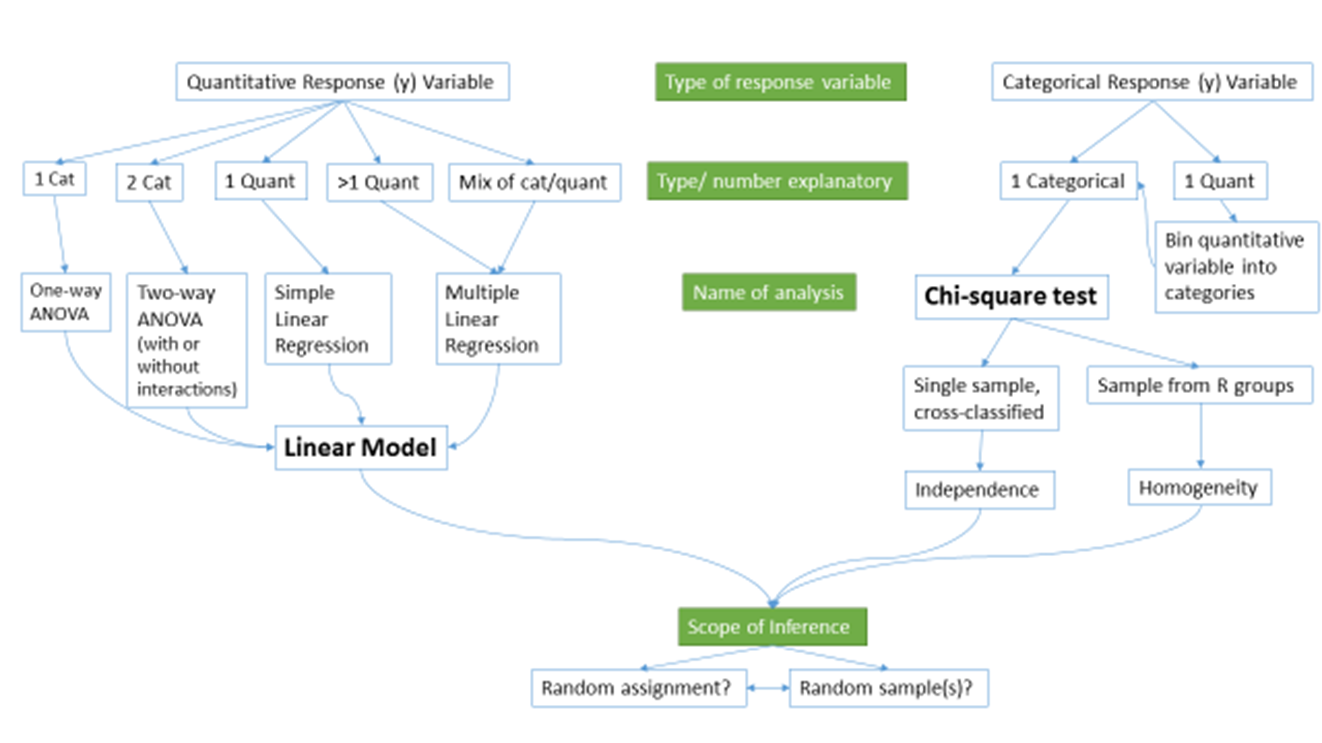
\includegraphics{chapter0_files/image002.png}
\caption{\label{fig:Figure1}Flow chart of methods}
\end{figure}

We will be spending most of the semester working on methods for
quantitative response variables (the left side of Figure
\ref{fig:Figure1} covered in Chapters \ref{chapter2}, \ref{chapter3},
\ref{chapter4}, \ref{chapter6}, \ref{chapter7}, and \ref{chapter8}) and
stepping over to handle the situation with a categorical response
variable (right side of Figure \ref{fig:Figure1} that is discussed in
Chapter \ref{chapter5}). Chapter \ref{chapter9} contains case studies
illustrating all the methods discussed previously, providing a final
opportunity to explore additional examples that illustrate how finding
your way through the paths in Figure \ref{fig:Figure1} leads to the
appropriate analysis.

The first topics (Chapters \ref{chapter1}, and \ref{chapter2}) will be
more familiar as we start with single and two group situations with a
quantitative response. In your previous statistics course, you should
have seen methods for estimating and quantifying uncertainty for the
mean of a single group and for differences in the means of two groups.
Once we have briefly reviewed these methods and introduced the
statistical software that we will use throughout the course, we will
consider the first new statistical material in Chapter \ref{chapter3}.
It involves the situation with a quantitative response variable where
there are more than 2 groups to compare -- this is what we call the
\textbf{\emph{One-Way ANOVA}} situation. It generalizes the
2-independent sample hypothesis test to handle situations where more
than 2 groups are being studied. When we learn this method, we will
begin discussing model assumptions and methods for assessing those
assumptions that will be present in every analysis involving a
quantitative response. The \textbf{\emph{Two-Way ANOVA}} (Chapter
\ref{chapter3}) considers situations with two categorical explanatory
variables and a quantitative response. To make this somewhat concrete,
suppose we are interested in assessing differences in, say, the
\emph{yield} of wheat from a field based on the amount of
\emph{fertilizer} applied(none, low, or high) and \emph{variety} of
wheat (two types). Here, \emph{yield} is a quantitative response
variable that might be measured in bushels per acre and there are two
categorical explanatory variables, \emph{fertilizer}, with 3 levels, and
\emph{variety}, with two levels. In this material, we introduce the idea
of an \textbf{\emph{interaction}} between the two explanatory variables:
the relationship between one categorical variable and the mean of the
response changes depending on the levels of the other categorical
variable. For example, extra fertilizer might enhance the growth of one
variety and hinder the growth of another so we would say that
\emph{fertilizer} has different impacts based this interaction may or
may not actually be present, we will consider two versions of the model
in Two-Way ANOVAs, what are called the \textbf{\emph{additive}} (no
interaction) and the \textbf{\emph{interaction}} models.

Following the methods for two categorical variables and a quantitative
response, we explore a method for analyzing data where the response is
categorical, called the \textbf{\emph{Chi-square test}} in Chapter
\ref{chapter5}. This most closely matches the One-Way ANOVA situation
with a single categorical explanatory variable, except now the response
variable is categorical. For example, we will assess whether taking a
drug (vs taking a \textbf{\emph{placebo}}\footnote{A
  \textbf{\emph{placebo}} is a treatment level designed to mimic the
  potentially efficacious level(s) but that can have no actual effect.
  The \textbf{\emph{placebo effect}} is the effect that thinking that an
  effective treatment was received has on subjects. There are other
  related issues in performing experiments like the
  \textbf{\emph{Hawthorne}} or observer \textbf{\emph{effect}} where
  subjects modify behavior because they are being observed.}) has an
\textbf{\emph{effect}}\footnote{We will reserve the term ``effect'' for
  situations where we could potentially infer causal impacts on the
  response of the explanatory variable which occurs in situations where
  the levels of the explanatory variable are randomly assigned to the
  subjects.} on the type of improvement the subjects demonstrate. There
are two different scenarios for study design that impact the analysis
technique and hypotheses tested in Chapter \ref{chapter5}. If the
explanatory variable reflects the group that subjects were obtained
from, either through randomization of the treatment level to the
subjects or by taking samples from separate populations, this is called
a \textbf{\emph{Chi-square Homogeneity Test}}. It is also possible to
obtain a single sample from a population and then obtain information on
the levels of the explanatory variable for each subject. We will analyze
these results using what is called a \textbf{\emph{Chi-square
Independence Test}}. They both use the same test statistic but we use
slightly different graphics and are testing different hypotheses in
these two related situations. Figure \ref{fig:Figure1} also shows that
if we had a quantitative explanatory variable and a categorical response
that we would need to ``bin'' or create categories of responses from the
quantitative variable to use the Chi-square testing methods.

If the predictor and response variables are both quantitative, we start
with scatterplots, correlation, and \textbf{\emph{simple linear
regression}} models (Chapters \ref{chapter6} and \ref{chapter7}) --
things you should have seen, at least to some degree, previously. The
biggest differences here will be the depth of exploration of diagnostics
and inferences for this model and discussions of transformations of
variables. If there is more than one explanatory variable, then we say
that we are doing \textbf{\emph{multiple linear regression}} (Chapter
\ref{chapter8}) -- the ``multiple'' part of the name reflects that there
will be more than one explanatory variable. We use the same name if we
have a mix of categorical and quantitative predictor variables but there
are some new issues in setting up the models and interpreting the
coefficients that we need to consider. In the situation with one
categorical predictor and one quantitative predictor, we revisit the
idea of an interaction. It allows us to consider situations where the
estimated relationship between a quantitative predictor and the mean
response varies among different levels of the categorical variable.

By the end of Chapter \ref{chapter9} you should be able to identify,
perform using the statistical software R \citep{R-base}, and interpret
the results from each of these methods. There is a lot to learn, but
many of the tools for using R and interpreting results of the analyses
accumulate and repeat during the semester. If you work hard to
understand the initial methods, it will help you when the methods get
more complicated. You will likely feel like you are just starting to
learn how to use R at the end of the semester and for learning a new
language that is actually an accomplishment. We will just be taking you
on the first steps of a potentially long journey and it is up to you to
decide how much further you want to go with learning the software.

All the methods you will learn require you to carefully consider how the
data were collected, how that pertains to the population of interest,
and how that impacts the inferences that can be made. The
\textbf{\emph{scope of inference}} from the bottom of Figure
\ref{fig:Figure1} is our shorthand term for remembering to think about
two aspects of the study -- \textbf{\emph{random assignment}} and
\textbf{\emph{random sampling}}. In a given situation, you need to use
the description of the study to decide if the explanatory variable was
randomly assigned to study units (this allows for \textbf{\emph{causal
inferences}} if differences are detected) or not (so no causal
statements are possible). As an example, think about two studies, one
where students are randomly assigned to either get tutoring with their
statistics course or not and another where the students are asked at the
end of the semester whether they sought out tutoring or not. Suppose we
compare the final grades in the course for the two groups (tutoring/not)
and find a big difference. In the first study with random assignment, we
can say the tutoring caused the differences we observed. In the second,
we could only say that the tutoring was associated with differences but
because students self-selected the group they ended up in, we can't say
that the tutoring caused the differences. The other aspect of scope of
inference concerns random sampling: If the data were obtained using a
random sampling mechanism, then our inferences can be safely extended to
the population that the sample was taken from. However, if we have
non-random sample, our inference can only apply to the sample collected.
In the previous example, the difference would be studying a random
sample of students from the population of, say, Introductory Statistics
students at a university vs studying a sample of students that
volunteered for the research project, maybe for extra credit in the
class. We could still randomly assign them to tutoring/not but the
non-random sample would only lead to conclusions about those students
that volunteered. The most powerful scope of inference is when there are
randomly assigned levels of explanatory variables with a random sample
from population -- conclusions would be about causal impacts that would
happen in the population.

By the end of this material, you should have some basic R skills and
abilities to create basic ANOVA and Regression models, as well as to
handle Chi-squared testing situations. Together, this should prepare you
for future statistics courses or for other situations where you are
expected to be able to identify an appropriate analysis, do the
calculations for a given data set, and then effectively communicate
interpretations for the methods discussed here.

\section{Getting started in R}\label{getting-started-in-r}

You will need to download the statistical software package called R and
an enhanced interface to R called RStudio \citep{RStudio}. They are open
source and free to download and use (and will always be that way). This
means that the skills you learn now can follow you the rest of your
life. R is becoming the primary language of statistics and is being
adopted across academia, government, and businesses to help manage and
learn from the growing volume of data being obtained. Hopefully you will
get a sense of some of the power of R in this book.

The next pages will walk you through the process of getting the software
downloaded and provide you with an initial experience using RStudio to
do things that should look familiar even though the interface will be a
new experience. Do not expect to master R quickly -- it takes years
(sorry!) even if you know the statistical methods being used. We will
try to keep all your interactions with R code in a similar code format
and that should help you in learning how to use R as we move through
various methods. We will also usually provide you with example code.
Everyone that learns R starts with copying other people's code and then
making changes for specific applications -- so expect to go back to
examples from the text and focus on learning how to modify that code to
work for your particular data set. Only really experienced R users
``know'' functions without having to check other resources. After we
complete this basic introduction, Chapter \ref{chapter2} begins doing
more sophisticated things with R, allowing us to compare quantitative
responses from two groups, make some graphical displays, do hypothesis
testing and create confidence intervals in a couple of different ways.

You will have two downloading activities to complete before you can do
anything more than read this book\footnote{I recorded a video that walks
  through the material on the following pages that is available here:
  \url{https://camtasia.msu.montana.edu/Relay/Files/w76c139/RandRstudio_Final/RandRstudio_Final_-_20160715_130555_23.html}
  in the digital version of the book.}. First, you need to download R.
It is the engine that will do all the computing for us, but you will
only interact with it once. Go to \url{http://cran.rstudio.com} and
click on the ``\textbf{Download R for\ldots{}}'' button that corresponds
to your operating system. On the next page, click on ``\textbf{base}''
and then it will take you to a screen to download the most current
version of R that is compiled for your operating system, something like
``\textbf{Download R 3.3.1 for Windows}''. Click on that link and then
open the file you downloaded. You will need to select your preferred
language (choose English so your instructor can help you), then hit
``\textbf{Next}'' until it starts to unpack and install the program (all
the base settings will be fine). After you hit ``\textbf{Finish}'' you
will not do anything further with R directly.

Second, you need to download RStudio. It is an enhanced interface that
will make interacting with R less frustrating. To download RStudio, go
to \url{http://www.rstudio.com/products/rstudio/download/} and select
the correct version under ``Installers for Supported Platforms'' for
your operating system. Download and then install RStudio using the
installer. From this point forward, you should only open RStudio; it
provides your interface with R. Note that both R and RStudio are updated
frequently (up to four times a year) and if you downloaded either more
than a few months previously, you should download the up-to-date
versions, especially if something you are trying to do is not working.
Sometimes code will not work in older versions of R and sometimes old
code won't work in new versions of R.\footnote{The need to keep the code
  up-to-date as R continues to evolve is one reason that this book is
  locally published and that this is the 3\(^{rd}\) version in three
  years\ldots{}}

To get started, we can complete some basic tasks in R using the RStudio
interface. When you open RStudio, you will see a screen like Figure
\ref{fig:Figure2}. The added annotation in this and the following
screen-grabs is there to help you get initially oriented to the software
interface. R is command-line software -- meaning that most of the time
you have to create code and then enter and execute it at a command
prompt to get any results. RStudio makes the management and execution of
that code more efficient than the basic version of R. In RStudio, the
lower left panel is called the ``console'' window and is where you can
type R code directly into R or where you will see the code you run and
(most importantly!) where the results of your executed commands will
show up. The most basic interaction with R is available once you get the
cursor active at the command prompt ``\textgreater{}'' by clicking in
that panel (look for a blinking vertical line). The upper left panel is
for writing, saving, and running your R code. Once you have code
available in this window, the ``Run'' button will execute the code for
the line that your cursor is on or for any text that you have
highlighted with your mouse. The ``data management'' or environment
panel is in the upper right, providing information on what data sets
have been loaded. It also contains the ``Import Dataset'' button that
provides the easiest way for you to read a data set into R so you can
analyze it. The lower right panel contains information on the
``Packages'' (additional code we will download and install to add
functionality to R) that are available and is where you will see plots
that you make and requests for ``Help'' on specific functions.



\begin{figure}
\centering
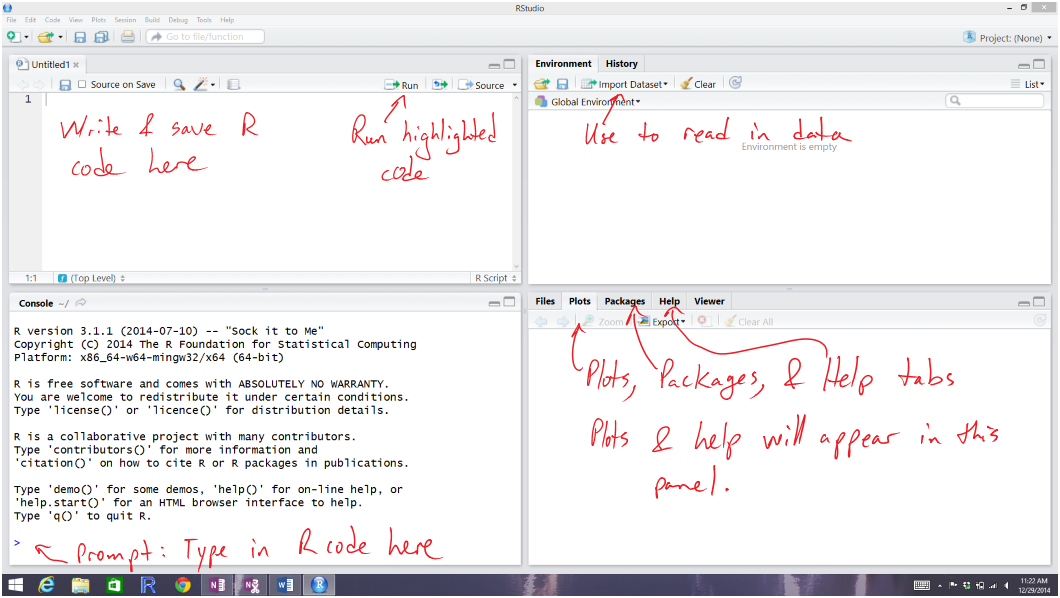
\includegraphics{chapter0_files/image003.png}
\caption{\label{fig:Figure2}Initial RStudio layout}
\end{figure}

As a first interaction with R we can use it as a calculator. To do this,
click near the command prompt (\texttt{\textgreater{}}) in the lower
left ``console'' panel, type 3+4, and then hit enter. It should look
like this:

\begin{Shaded}
\begin{Highlighting}[]
\OperatorTok{>}\StringTok{ }\DecValTok{3}\OperatorTok{+}\DecValTok{4}
\NormalTok{[}\DecValTok{1}\NormalTok{] }\DecValTok{7}
\end{Highlighting}
\end{Shaded}

You can do more interesting calculations, like finding the mean of the
numbers 3, 5, 7, and 8 by adding them up and dividing by 4:

\begin{Shaded}
\begin{Highlighting}[]
\OperatorTok{>}\StringTok{ }\NormalTok{(}\OperatorTok{-}\DecValTok{3}\OperatorTok{+}\DecValTok{5}\OperatorTok{+}\DecValTok{7}\OperatorTok{+}\DecValTok{8}\NormalTok{)}\OperatorTok{/}\DecValTok{4}
\NormalTok{[}\DecValTok{1}\NormalTok{] }\DecValTok{4}\NormalTok{. }\DecValTok{25}
\end{Highlighting}
\end{Shaded}

Note that the parentheses help R to figure out your desired order of
operations. If you drop that grouping, you get a very different (and
wrong!) result:

\begin{Shaded}
\begin{Highlighting}[]
\OperatorTok{>}\StringTok{ }\OperatorTok{-}\DecValTok{3}\OperatorTok{+}\DecValTok{5}\OperatorTok{+}\DecValTok{7}\OperatorTok{+}\DecValTok{8}\OperatorTok{/}\DecValTok{4}
\NormalTok{[}\DecValTok{1}\NormalTok{] }\DecValTok{11}
\end{Highlighting}
\end{Shaded}

We could estimate the standard deviation similarly using the formula you
might remember from introductory statistics, but that will only work in
very limited situations. To use the real power of R this semester, we
need to work with data sets that store the Basically, we need to store
observations in named vectors (one dimensional arrays) that contain a
list of the observations. To create a vector containing the four numbers
and assign it to a variable named \emph{variable1}, we need to create a
vector using the function \texttt{c} which means ``combine the items''
that follow, if they are inside parentheses and have commas separating
the values, as follows:

\begin{Shaded}
\begin{Highlighting}[]
\OperatorTok{>}\StringTok{ }\KeywordTok{c}\NormalTok{(}\OperatorTok{-}\DecValTok{3}\NormalTok{, }\DecValTok{5}\NormalTok{, }\DecValTok{7}\NormalTok{, }\DecValTok{8}\NormalTok{)}
\NormalTok{[}\DecValTok{1}\NormalTok{] }\OperatorTok{-}\DecValTok{3} \DecValTok{5} \DecValTok{7} \DecValTok{8}
\end{Highlighting}
\end{Shaded}

To get this vector stored in a variable called \emph{variable1} we need
to use the assignment operator, \texttt{\textless{}-} (read as ``stored
as'') that assigns the information on the right into the variable that
you are creating on the left.

\begin{Shaded}
\begin{Highlighting}[]
\OperatorTok{>}\StringTok{ }\NormalTok{variable1 <-}\StringTok{ }\KeywordTok{c}\NormalTok{(}\OperatorTok{-}\DecValTok{3}\NormalTok{, }\DecValTok{5}\NormalTok{, }\DecValTok{7}\NormalTok{, }\DecValTok{8}\NormalTok{)}
\end{Highlighting}
\end{Shaded}

In R, the assignment operator, \texttt{\textless{}-}, is created by
typing a ``less than'' symbol \texttt{\textless{}} followed by a
``minus'' sign (\texttt{-}) ever want to see what numbers are residing
in an object in R, just type its name and hit \emph{enter}. You can see
how that variable contains the same information that was initially
generated by \texttt{c(-3,\ 5,\ 7,\ 8)} but is easier to access since we
just need the text for the variable name representing that vector.

\begin{Shaded}
\begin{Highlighting}[]
\OperatorTok{>}\StringTok{ }\NormalTok{variable1}
\NormalTok{[}\DecValTok{1}\NormalTok{] }\OperatorTok{-}\DecValTok{3} \DecValTok{5} \DecValTok{7} \DecValTok{8}
\end{Highlighting}
\end{Shaded}

With the data stored in a variable, wean use functions such as
\texttt{mean} and \texttt{sd} to find the mean and standard deviation of
the observations contained in \texttt{variable1} :

\begin{Shaded}
\begin{Highlighting}[]
\OperatorTok{>}\StringTok{ }\KeywordTok{mean}\NormalTok{(variable1)}
\NormalTok{[}\DecValTok{1}\NormalTok{] }\FloatTok{4.25}
\OperatorTok{>}\StringTok{ }\KeywordTok{sd}\NormalTok{(variable1)}
\NormalTok{[}\DecValTok{1}\NormalTok{] }\FloatTok{4.99166}
\end{Highlighting}
\end{Shaded}

When dealing with real data, we will often have information about more
than one variable. We could enter all observations by hand for each
variable but this is prone to error and onerous for all but the smallest
data sets. If you are to ever utilize the power of statistics in the
evolving data-centered world, data management has to be accomplished in
a more sophisticated way. While you can manage data sets quite
effectively in R, it is often easiest to start with your data set in
something like Microsoft Excel or OpenOffice's Calc. You want to make
sure that observations are in the rows and the names of variables are in
the columns and that there is no ``extra stuff'' in the spreadsheet. If
you have missing observations, they should be represented with blank
cells. The file should be saved as a ``.csv'' file (stands for
comma-separated values although Excel calls it ``CSV (Comma
Delimited)'', which basically strips off some of the junk that Excel
adds to the necessary information in the file. Excel will tell you that
this is a bad idea, but it actually creates a more stable archival
format and one that R can use directly\footnote{There are ways to read
  ``.xls'' and ``.xlsx'' files directly into R but to handle multiple
  sheets they are more complicated and not as stable across operating
  systems as the simpler version we recommend.}.

With data set converted to a CSV file, we need to read the data set into
R. There are two ways to do this, either using the point-and-click GUI
in RStudio (click the ``Import Data Set'' button in the upper right
``Environment'' panel as indicated in Figure \ref{fig:Figure2}) or
modifying the

\texttt{read.csv} function to find the file of interest. To practice
this, you can download an Excel (.xls) file from
\url{http://www.math.montana.edu/courses/s217/documents/treadmill.xls}
31 males that volunteered for a study on methods for measuring fitness
\citep{Westfall1993}. In the spreadsheet, you will find a data set that
starts and ends with the following information (only results for
Subjects 1, 2, 30, and 31 shown here):

\begin{longtable}[]{@{}lllrrlrr@{}}
\toprule
\begin{minipage}[b]{0.07\columnwidth}\raggedright\strut
Sub- ject\strut
\end{minipage} & \begin{minipage}[b]{0.10\columnwidth}\raggedright\strut
Tread- MillOx\strut
\end{minipage} & \begin{minipage}[b]{0.14\columnwidth}\raggedright\strut
TreadMill- MaxPulse\strut
\end{minipage} & \begin{minipage}[b]{0.09\columnwidth}\raggedleft\strut
RunTime\strut
\end{minipage} & \begin{minipage}[b]{0.10\columnwidth}\raggedleft\strut
RunPulse\strut
\end{minipage} & \begin{minipage}[b]{0.08\columnwidth}\raggedright\strut
Rest Pulse\strut
\end{minipage} & \begin{minipage}[b]{0.15\columnwidth}\raggedleft\strut
BodyWeight\strut
\end{minipage} & \begin{minipage}[b]{0.04\columnwidth}\raggedleft\strut
Age\strut
\end{minipage}\tabularnewline
\midrule
\endhead
\begin{minipage}[t]{0.07\columnwidth}\raggedright\strut
1\strut
\end{minipage} & \begin{minipage}[t]{0.10\columnwidth}\raggedright\strut
60.05\strut
\end{minipage} & \begin{minipage}[t]{0.14\columnwidth}\raggedright\strut
186\strut
\end{minipage} & \begin{minipage}[t]{0.09\columnwidth}\raggedleft\strut
8.63\strut
\end{minipage} & \begin{minipage}[t]{0.10\columnwidth}\raggedleft\strut
170\strut
\end{minipage} & \begin{minipage}[t]{0.08\columnwidth}\raggedright\strut
48\strut
\end{minipage} & \begin{minipage}[t]{0.15\columnwidth}\raggedleft\strut
81.87\strut
\end{minipage} & \begin{minipage}[t]{0.04\columnwidth}\raggedleft\strut
38\strut
\end{minipage}\tabularnewline
\begin{minipage}[t]{0.07\columnwidth}\raggedright\strut
2\strut
\end{minipage} & \begin{minipage}[t]{0.10\columnwidth}\raggedright\strut
59.57\strut
\end{minipage} & \begin{minipage}[t]{0.14\columnwidth}\raggedright\strut
172\strut
\end{minipage} & \begin{minipage}[t]{0.09\columnwidth}\raggedleft\strut
8.17\strut
\end{minipage} & \begin{minipage}[t]{0.10\columnwidth}\raggedleft\strut
166\strut
\end{minipage} & \begin{minipage}[t]{0.08\columnwidth}\raggedright\strut
40\strut
\end{minipage} & \begin{minipage}[t]{0.15\columnwidth}\raggedleft\strut
68.15\strut
\end{minipage} & \begin{minipage}[t]{0.04\columnwidth}\raggedleft\strut
42\strut
\end{minipage}\tabularnewline
\begin{minipage}[t]{0.07\columnwidth}\raggedright\strut
\ldots{}\strut
\end{minipage} & \begin{minipage}[t]{0.10\columnwidth}\raggedright\strut
\ldots{}\strut
\end{minipage} & \begin{minipage}[t]{0.14\columnwidth}\raggedright\strut
\ldots{}\strut
\end{minipage} & \begin{minipage}[t]{0.09\columnwidth}\raggedleft\strut
\ldots{}\strut
\end{minipage} & \begin{minipage}[t]{0.10\columnwidth}\raggedleft\strut
\ldots{}\strut
\end{minipage} & \begin{minipage}[t]{0.08\columnwidth}\raggedright\strut
\ldots{}\strut
\end{minipage} & \begin{minipage}[t]{0.15\columnwidth}\raggedleft\strut
\ldots{}\strut
\end{minipage} & \begin{minipage}[t]{0.04\columnwidth}\raggedleft\strut
\ldots{}\strut
\end{minipage}\tabularnewline
\begin{minipage}[t]{0.07\columnwidth}\raggedright\strut
30\strut
\end{minipage} & \begin{minipage}[t]{0.10\columnwidth}\raggedright\strut
39.2\strut
\end{minipage} & \begin{minipage}[t]{0.14\columnwidth}\raggedright\strut
172\strut
\end{minipage} & \begin{minipage}[t]{0.09\columnwidth}\raggedleft\strut
12.88\strut
\end{minipage} & \begin{minipage}[t]{0.10\columnwidth}\raggedleft\strut
168\strut
\end{minipage} & \begin{minipage}[t]{0.08\columnwidth}\raggedright\strut
44\strut
\end{minipage} & \begin{minipage}[t]{0.15\columnwidth}\raggedleft\strut
91.63\strut
\end{minipage} & \begin{minipage}[t]{0.04\columnwidth}\raggedleft\strut
54\strut
\end{minipage}\tabularnewline
\begin{minipage}[t]{0.07\columnwidth}\raggedright\strut
31\strut
\end{minipage} & \begin{minipage}[t]{0.10\columnwidth}\raggedright\strut
37.39\strut
\end{minipage} & \begin{minipage}[t]{0.14\columnwidth}\raggedright\strut
192\strut
\end{minipage} & \begin{minipage}[t]{0.09\columnwidth}\raggedleft\strut
14.03\strut
\end{minipage} & \begin{minipage}[t]{0.10\columnwidth}\raggedleft\strut
186\strut
\end{minipage} & \begin{minipage}[t]{0.08\columnwidth}\raggedright\strut
56\strut
\end{minipage} & \begin{minipage}[t]{0.15\columnwidth}\raggedleft\strut
87.66\strut
\end{minipage} & \begin{minipage}[t]{0.04\columnwidth}\raggedleft\strut
45\strut
\end{minipage}\tabularnewline
\bottomrule
\end{longtable}

The variables contain information on the subject number
(\emph{Subject}), subjects' treadmill oxygen consumption
(\emph{TreadMillOx}, in ml per kg per minute) and maximum pulse rate
(\emph{TreadMillMaxPulse}, in beats per minute), time to run 1.5 miles
(\emph{Run Time}, in minutes), maximum pulse during 1.5 mile run
(\emph{RunPulse}, in beats per minute), resting pulse rate
(\emph{RestPulse}, beats per minute), Body Weight (\emph{BodyWeight}, in
kg), and \emph{Age} (in years). Open the file in Excel or equivalent
software and then save it as a .csv file in a location you can find on
your computer. Then go to RStudio and click on \textbf{File} , then
\textbf{Import Dataset} , then \textbf{From CSV\ldots{}}\footnote{If you
  are having trouble getting the file converted and read into R, copy
  and run the following code:
  \texttt{treadmill\ \textless{}-\ read.csv("http://www.math.montana.edu/courses/s217/documents/treadmill.csv",\ header=T)}.}
Find your file and check ``\textbf{Import}''. R will store the data set
as an object named whatever the .csv file was named. You could use
another name as well, but it is often easiest just to keep the data set
name in R related to the original file name. You should see some text
appear in the console (lower left panel) like in Figure
\ref{fig:Figure3}. The text that is created will look something like the
following -- if you had stored the file in a drive labeled D:, it would
be:

\begin{Shaded}
\begin{Highlighting}[]
\NormalTok{treadmill <-}\StringTok{ }\KeywordTok{read.csv}\NormalTok{(}\StringTok{"D:/treadmill.csv"}\NormalTok{)}
\end{Highlighting}
\end{Shaded}

What is put inside the \texttt{"\ "} will depend on the location and
name of your saved .csv file. A version of the data set in what looks
like a spreadsheet will appear in the upper left window due to the
second line of code (\texttt{View(treadmill})).



\begin{figure}
\centering
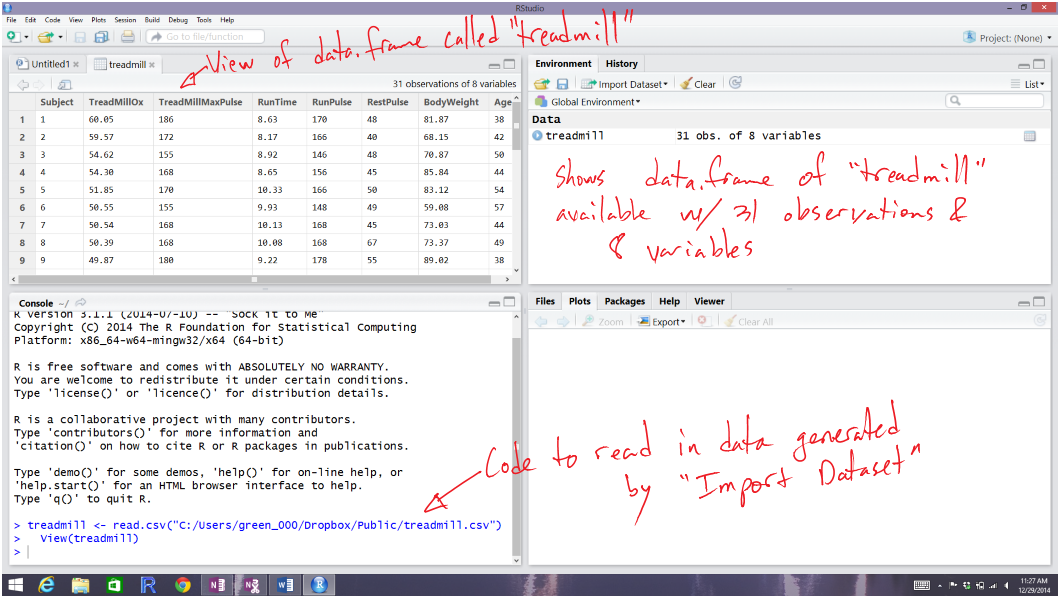
\includegraphics{chapter0_files/image005.png}
\caption{\label{fig:Figure3}RStudio with initial data set loaded}
\end{figure}

Just directly typing (or using) a line of code like this is actually the
other way that we can read in files. If you choose to use the text-only
interface, then you need to tell R where to look in your computer to
find the data file. \texttt{read.csv} is a function that takes a path as
an argument. To use it, specify the path to your data file, put quotes
around it, and put it as the input to \texttt{read.csv(...)}. For some
examples later in the book, you will be able to copy a command like this
from the text and read data sets and other code directly from my the
course folder, assuming you are connected to the internet.

To verify that you read the data set in correctly, it is always good to
check its contents. We can view the first and last rows in the data set
using the \texttt{head} and \texttt{tail} functions on the data set,
which show the following results for the \texttt{treadmill} data. Note
that you will sometimes need to resize the console window in RStudio to
get all the columns to display in a single row which can be performed by
dragging the gray bars that separate the panels.

\begin{Shaded}
\begin{Highlighting}[]
\KeywordTok{head}\NormalTok{(treadmill)}
\end{Highlighting}
\end{Shaded}

\begin{verbatim}
##   Subject TreadMillOx TreadMillMaxPulse RunTime RunPulse RestPulse
## 1       1       60.05               186    8.63      170        48
## 2       2       59.57               172    8.17      166        40
## 3       3       54.62               155    8.92      146        48
## 4       4       54.30               168    8.65      156        45
## 5       5       51.85               170   10.33      166        50
## 6       6       50.55               155    9.93      148        49
##   BodyWeight Age
## 1      81.87  38
## 2      68.15  42
## 3      70.87  50
## 4      85.84  44
## 5      83.12  54
## 6      59.08  57
\end{verbatim}

\begin{Shaded}
\begin{Highlighting}[]
\KeywordTok{tail}\NormalTok{(treadmill)}
\end{Highlighting}
\end{Shaded}

\begin{verbatim}
##    Subject TreadMillOx TreadMillMaxPulse RunTime RunPulse RestPulse
## 26      26       44.61               182   11.37      178        62
## 27      27       40.84               172   10.95      168        57
## 28      28       39.44               176   13.08      174        63
## 29      29       39.41               176   12.63      174        58
## 30      30       39.20               172   12.88      168        44
## 31      31       37.39               192   14.03      186        56
##    BodyWeight Age
## 26      89.47  44
## 27      69.63  51
## 28      81.42  44
## 29      73.37  57
## 30      91.63  54
## 31      87.66  45
\end{verbatim}

While not always required, for many of the analyses, we will tap into a
large suite of additional functions available in R packages by
``installing'' (basically downloading) and then ``loading'' the
packages. There are some packages that we will use frequently, starting
with the \texttt{mosaic} package \citep{R-mosaic}. To install an R
package, go to the \textbf{Packages} tab in the lower right panel of
RStudio. Click on the \textbf{Install} button and then type in the name
of the package in the box (here type in \texttt{mosaic}). RStudio will
try to auto-complete the package name you are typing which should help
you make sure you got it typed correctly. This will be the first of
\emph{many} times that we will mention that R is case sensitive -- in
other words, \texttt{Mosaic} is different from \texttt{mosaic} in R
syntax and this sort of thing applies to everything you do in R. You
should only need to install each R package once on a given computer. If
you ever see a message that R can't find a package, make sure it appears
in the list in the \textbf{Packages} tab and if it doesn't, repeat the
previous steps to install it.

After installing the package, we need to load it to make it active in a
given work session. Go to the command prompt and type (or copy and
paste) \texttt{require(mosaic)} :

\begin{Shaded}
\begin{Highlighting}[]
\KeywordTok{require}\NormalTok{(mosaic)}
\end{Highlighting}
\end{Shaded}

You may see a warning message about versions of the package and versions
of R -- this is \emph{usually} something you can ignore. Other warning
messages could be more ominous for proceeding but before getting too
concerned, there are couple of basic things to check. First, double
check that the package is installed (see previous steps). Second, check
for typographical errors in your code -- especially for mis-spellings or
unintended capitalization. If you are still having issues, try repeating
the installation process. If that fails, find someone more used to using
R to help you (for example in the Math Learning Center or by emailing
your instructor)\footnote{Most computer lab computers at Montana State
  University have RStudio installed and so provide another venue to try
  this where the software is already installed.}.

To help you go from basic to intermediate R usage and especially to help
with more complicated problems, you will want to learn how to manage and
save your R code. The best way to do this is using the upper left panel
in RStudio using what are called R Scripts, which are files that have a
file extension of ``.R''. To start a new ``.R''" file to store your
code, click on \textbf{File}, then \textbf{New File}, then \textbf{R
Script}. This will create a blank page to enter and edit code -- then
save the file as MyFileName.R in your preferred location. Saving your
code will mean that you can return to where you last were working by
simply re-running the saved script file. With code in the script window,
you can place the cursor on a line of code or highlight a chunk of code
and hit the ``Run'' button on the upper part of the panel. It will
appear in the console with results just like what you would obtain if
you typed it after the command prompt and hit enter for each line.

Figure \ref{fig:Figure4} shows the screen with the code used in this
section in the upper left panel, saved in file called Ch0.R, with the
results of highlighting and executing the first section of code using
the ``Run'' button.



\begin{figure}
\centering
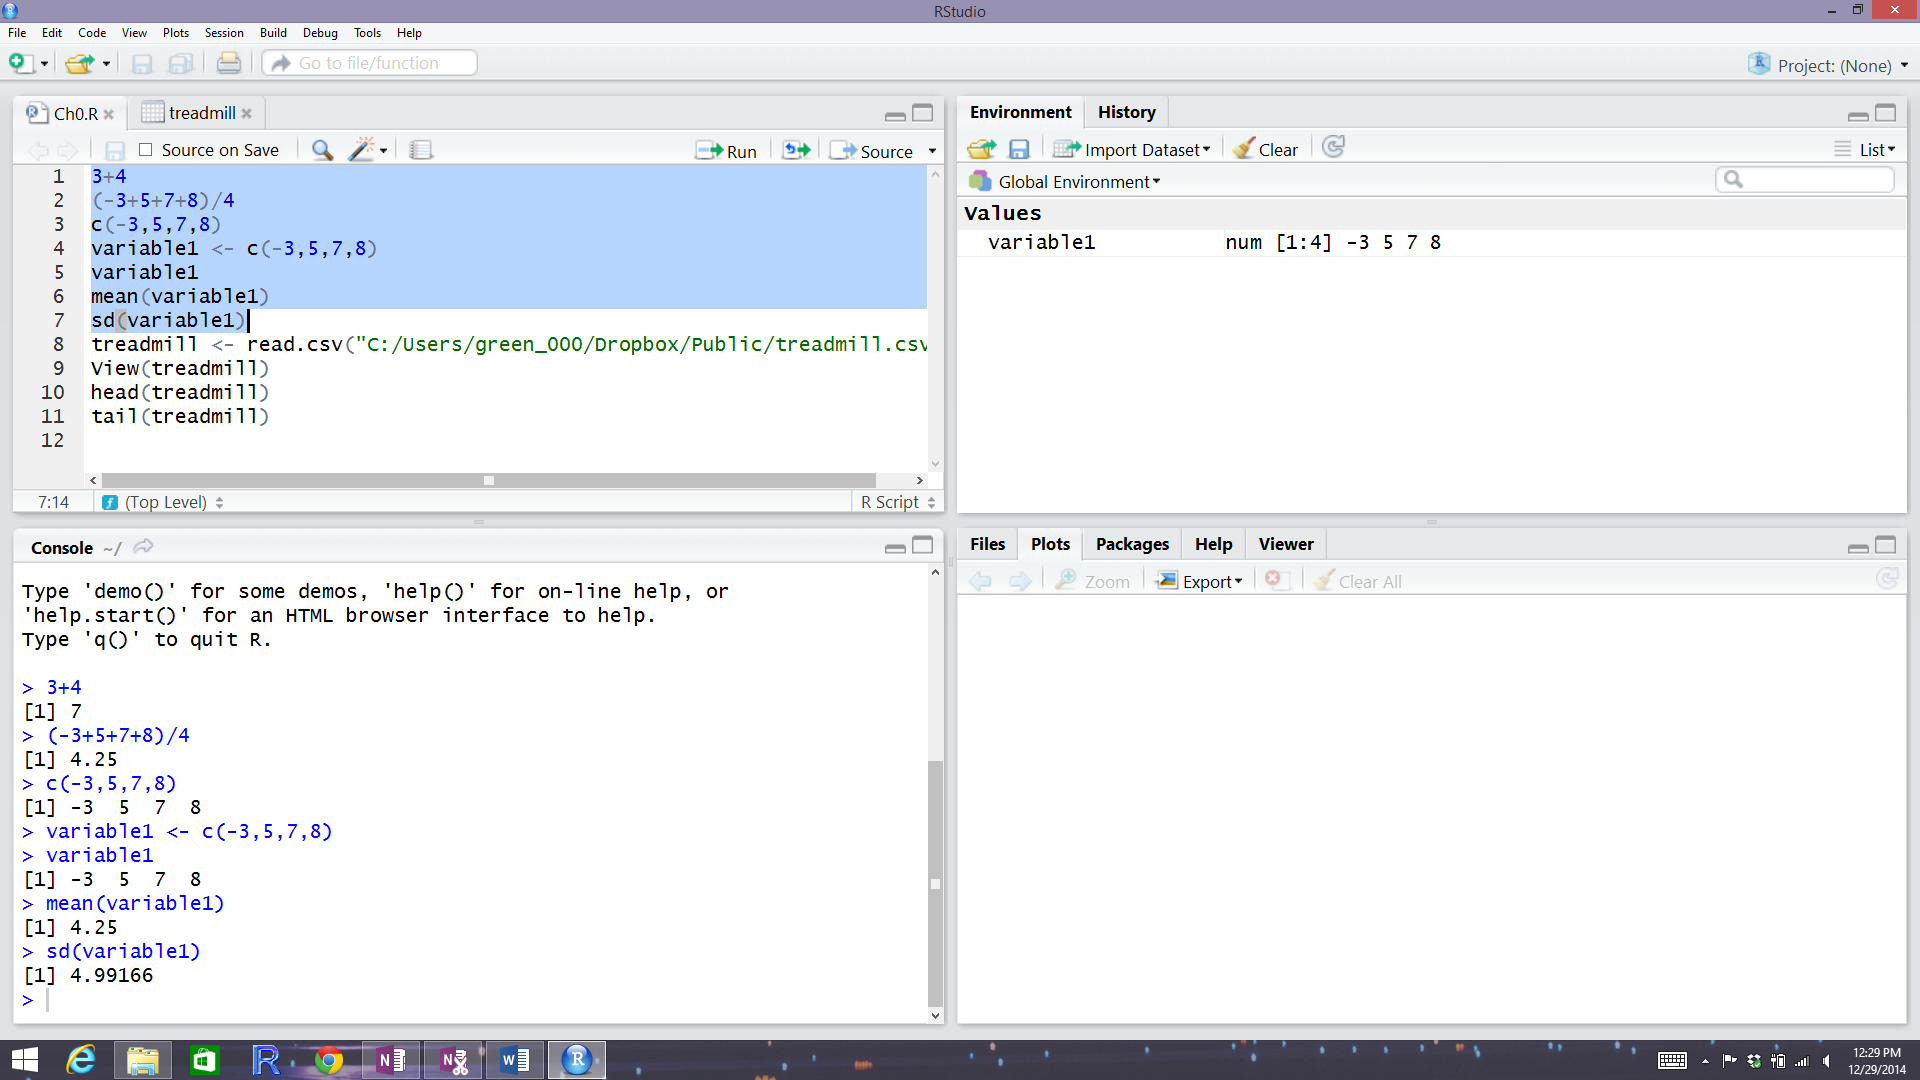
\includegraphics{chapter0_files/image006.png}
\caption{\label{fig:Figure4}RStudio with highlighted code run}
\end{figure}

\section{Basic summary statistics, histograms, and boxplots using
R}\label{basic-summary-statistics-histograms-and-boxplots-using-r}

With RStudio running, the \texttt{mosaic} package loaded, a place to
write and save code, and the \texttt{treadmill} data set loaded, we can
(finally!) start to summarize the results of the study. The
\texttt{treadmill} object is what R calls a
\textbf{\emph{data.frame}}\footnote{Data frames in R are objects that
  can contain both categorical and quantitative variables on your n
  subjects with a name for each variable that is also the name of each
  column in a matrix. Each subject is a row of the data set.} and
contains columns corresponding to each variable in the spreadsheet.
Every function in R will involve specifying the variable(s) of interest
and how you want to use them. To access a particular variable (column)
in a data.frame, you can use a \$ between the data.frame name and the
name of the variable of interest, generically as
\texttt{dataframename\$variablename}. To identify the \texttt{RunTime}
variable here it would be \texttt{treadmill\$RunTime}. In the command
line it would look like:

\begin{Shaded}
\begin{Highlighting}[]
\NormalTok{treadmill}\OperatorTok{$}\NormalTok{RunTime}
\end{Highlighting}
\end{Shaded}

\begin{verbatim}
##  [1]  8.63  8.17  8.92  8.65 10.33  9.93 10.13 10.08  9.22  8.95 10.85
## [12]  9.40 11.50 10.50 10.60 10.25 10.00 11.17 10.47 11.95  9.63 10.07
## [23] 11.08 11.63 11.12 11.37 10.95 13.08 12.63 12.88 14.03
\end{verbatim}

Just as in the previous section, we can generate summary statistics
using functions like \texttt{mean} and \texttt{sd} by running them on a
specific variable:

\begin{Shaded}
\begin{Highlighting}[]
\KeywordTok{mean}\NormalTok{(treadmill}\OperatorTok{$}\NormalTok{RunTime)}
\end{Highlighting}
\end{Shaded}

\begin{verbatim}
## [1] 10.58613
\end{verbatim}

\begin{Shaded}
\begin{Highlighting}[]
\KeywordTok{sd}\NormalTok{(treadmill}\OperatorTok{$}\NormalTok{RunTime)}
\end{Highlighting}
\end{Shaded}

\begin{verbatim}
## [1] 1.387414
\end{verbatim}

And now we know that the average running time for 1.5 miles for the
subjects in the study was 10.6 minutes with a standard deviation (SD) of
1.39 minutes. But you should remember that the mean and SD are only
appropriate summaries if the distribution is roughly
\textbf{\emph{symmetric}} (both sides of the distribution are
approximately the same). The \texttt{mosaic} package provides a useful
function called \texttt{favstats} that provides the mean and SD as well
as the \textbf{\emph{5 number summary}} : the minimum (\texttt{min}),
the first quartile (\texttt{Q1}, the 25\(^{th}\) percentile), the median
(50\(^{th}\) percentile), the third quartile (\texttt{Q3} , the
75\(^{th}\) percentile), and the maximum (\texttt{max}). It also
provides the number of observations (\texttt{n}) which was 31, as noted
above, and a count of whether any missing values were encountered
(\texttt{missing}), which was 0 here since all subjects had measurements
available on this variable.

\begin{Shaded}
\begin{Highlighting}[]
\KeywordTok{favstats}\NormalTok{(treadmill}\OperatorTok{$}\NormalTok{RunTime)}
\end{Highlighting}
\end{Shaded}

\begin{verbatim}
##   min   Q1 median    Q3   max     mean       sd  n missing
##  8.17 9.78  10.47 11.27 14.03 10.58613 1.387414 31       0
\end{verbatim}

We are starting to get somewhere with understanding that the runners
were somewhat fit with worst runner covering 1.5 miles in 14 minutes
(the equivalent of a 9.3 minute mile) and the best running at a 5.4
minute mile pace. The limited variation in the results suggests that the
sample was obtained from a restricted group with somewhat common
characteristics. When you explore the ages and weights of the subjects
in the Practice Problems in Section 0.5, you will get even more
information about how similar all the subjects in this study were.

A graphical display of these results will help us to assess the shape of
the distribution of run times -- including considering the potential for
the presence of a \textbf{\emph{skew}} (whether the right or left tail
of the distribution is noticeably more spread out with left skew meaning
that the left tail is more spread out than the right tail) and
\textbf{\emph{outliers}} (unusual observations). A
\textbf{\emph{histogram }} is a good place to start. Histograms display
connected bars with counts of observations defining the height of bars
based on a set of bins of values of the quantitative variable. We will
apply the \texttt{hist} function to the \texttt{RunTime} variable, which
produces Figure \ref{fig:Figure5}.




\begin{figure}
\centering
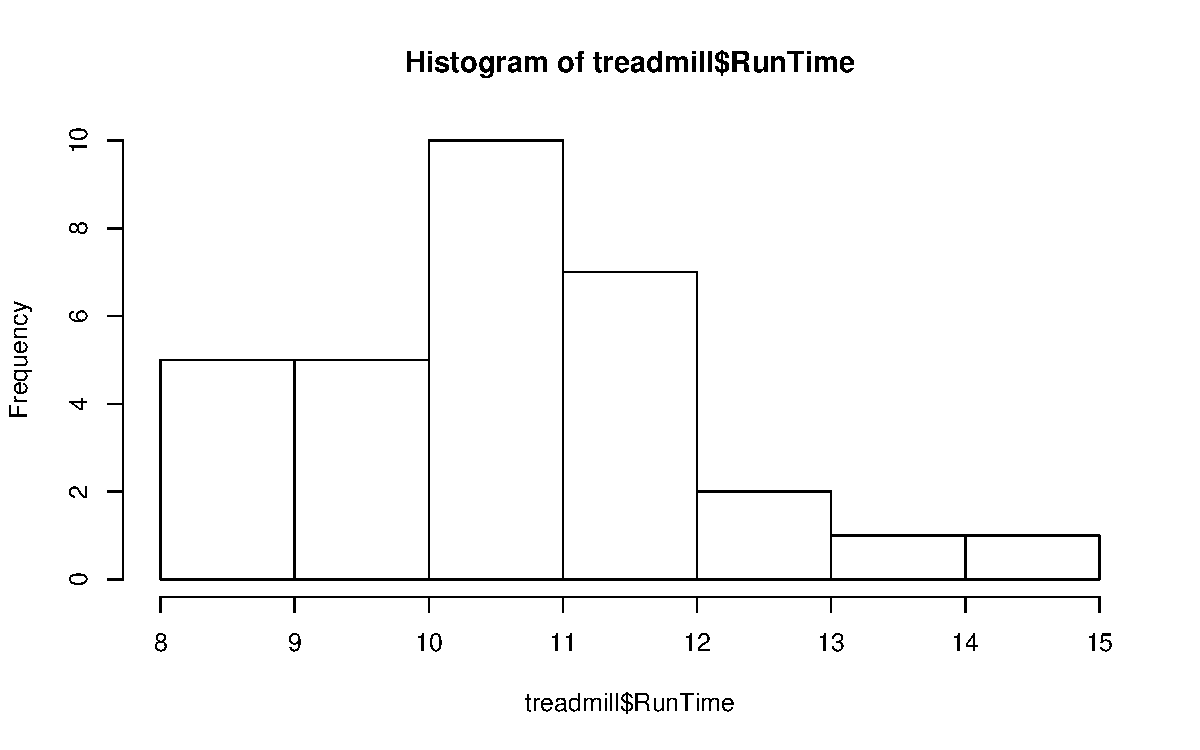
\includegraphics{01-preface_files/figure-latex/Figure5-1.pdf}
\caption{\label{fig:Figure5}Histogram of Run Times \#(minutes) of n=31 subjects in
Treadmill study.}
\end{figure}

I used the \textbf{Export} button found above the plot, followed by
\textbf{Copy to Clipboard} and clicking on the \textbf{Copy Plot}
button. Then if you open your favorite word-processing program, you
should be able to paste it into a document for writing reports that
include the figures. You can see the first parts of this process in the
screen grab in Figure \ref{fig:Figure6}.



\begin{figure}
\centering
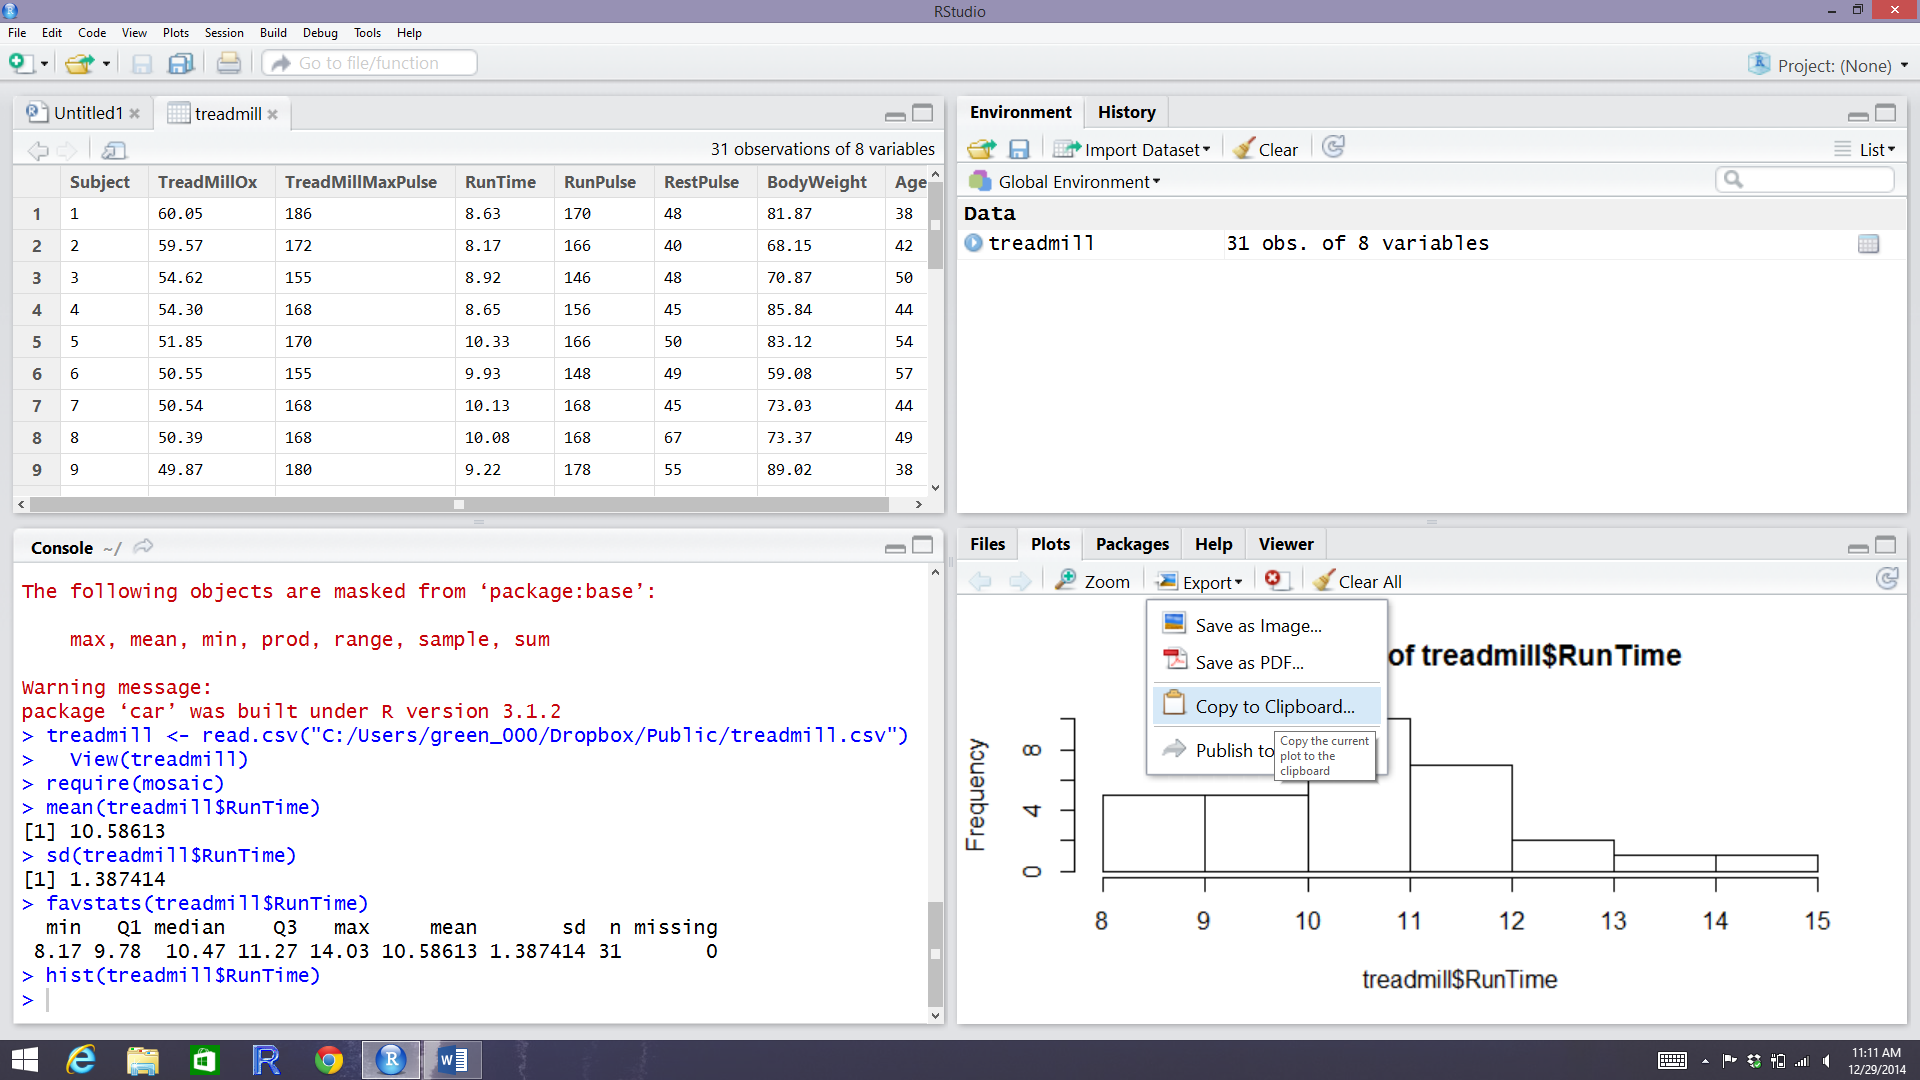
\includegraphics{chapter0_files/image010.png}
\caption{\label{fig:Figure6}RStudio while in the process of copying the histogram}
\end{figure}

You can also directly save the figures as separate files using
\textbf{Save as Image} or \textbf{Save as PDF}and then insert them into
your word processing documents.

The function \texttt{hist} defaults into providing a histogram on the
\textbf{\emph{frequency}} (count) scale. In most R functions, there are
the default options that will occur if we don't make any specific
choices but we can override the default options if we desire. One option
we can modify here is to add labels to the bars to be able to see
exactly how many observations fell into each bar. Specifically, we can
turn the \texttt{labels} option ``on'' by making it true (``T'') by
adding \texttt{labels=T} to the previous call to the \texttt{hist}
function, separated by a comma:



\begin{Shaded}
\begin{Highlighting}[]
\KeywordTok{hist}\NormalTok{(treadmill}\OperatorTok{$}\NormalTok{RunTime, }\DataTypeTok{labels=}\NormalTok{T)}
\end{Highlighting}
\end{Shaded}

\begin{figure}
\centering
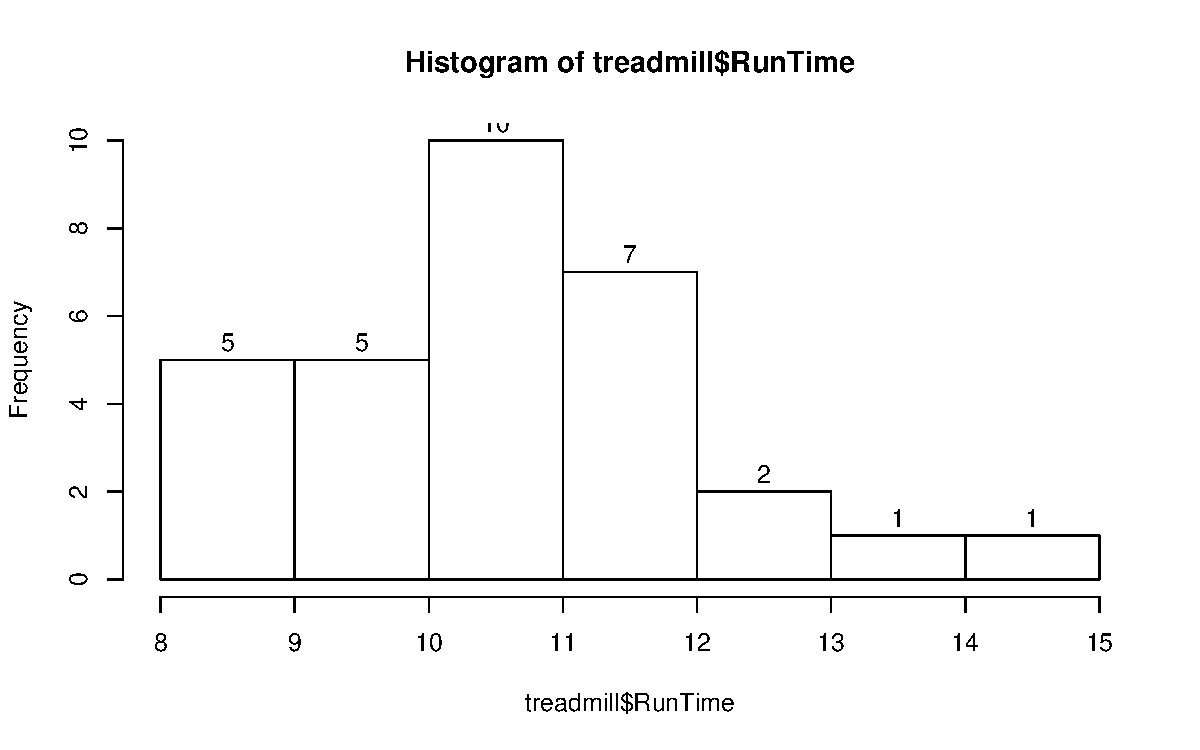
\includegraphics{01-preface_files/figure-latex/Figure7-1.pdf}
\caption{\label{fig:Figure7}Histogram of \#Run Times with counts in bars labeled.}
\end{figure}

Based on this histogram, it does not appear that there any outliers in
the responses since there are no bars that are separated from the other
observations. However, the distribution does not look symmetric and
there might be a skew to the distribution. Specifically, it appears to
be \textbf{\emph{skewed right}} (the right tail is longer than the
left). But histograms can sometimes mask features of the data set by
binning observations and it is hard to find the percentiles accurately
from the plot.

When assessing outliers and skew, the \textbf{\emph{boxplot}} (or
\emph{Box and Whiskers} plot) can also be helpful (Figure
\ref{fig:Figure8}) to describe the shape of the distribution as it
displays the 5-number summary and will also indicate observations that
are ``far'' above the middle of the observations. R's \texttt{boxplot}
function uses the standard rule to indicate an observation as a
\textbf{\emph{potential outlier}} if it falls more than 1.5 times the
\textbf{\emph{IQR}} (Inter-Quartile Range, calculated as Q3-Q1) below Q1
or above Q3. The potential outliers are plotted with circles and the
\emph{Whiskers} (lines that extend from Q1 and Q3 typically to the
minimum and maximum) are shortened to only go as far as observations
that are within \(1.5*\)IQR of the upper and lower quartiles. The
\emph{box} part of the boxplot is a box that goes from Q1 to Q3 and the
median is displayed as a line somewhere inside the box\footnote{The
  median, quartiles and whiskers sometimes occur at the same values when
  there are many tied observations. If you can't see all the components
  of the boxplot, produce the numerical summary to help you understand
  what happened.}. Looking back at the summary statistics above, Q1=9.78
and Q3=11.27, providing an IQR of:

\begin{Shaded}
\begin{Highlighting}[]
\NormalTok{IQR <-}\StringTok{ }\FloatTok{11.27} \OperatorTok{-}\StringTok{ }\FloatTok{9.78}
\end{Highlighting}
\end{Shaded}

One observation (the maximum value of 14.03) is indicated as a potential
outlier based on this result by being larger than Q3 \(+1.5*\)IQR, which
was 13.505:

\begin{Shaded}
\begin{Highlighting}[]
\FloatTok{11.27} \OperatorTok{+}\StringTok{ }\FloatTok{1.5}\OperatorTok{*}\NormalTok{IQR}
\end{Highlighting}
\end{Shaded}

\begin{verbatim}
## [1] 13.505
\end{verbatim}

The boxplot also shows a slight indication of a right skew (skew towards
larger values) with the distance from the minimum to the median being
smaller than the distance from the median to the maximum. Additionally,
the distance from Q1 to the median is smaller than the distance from the
median to Q3. It is modest skew, but worth noting.



\begin{figure}
\centering
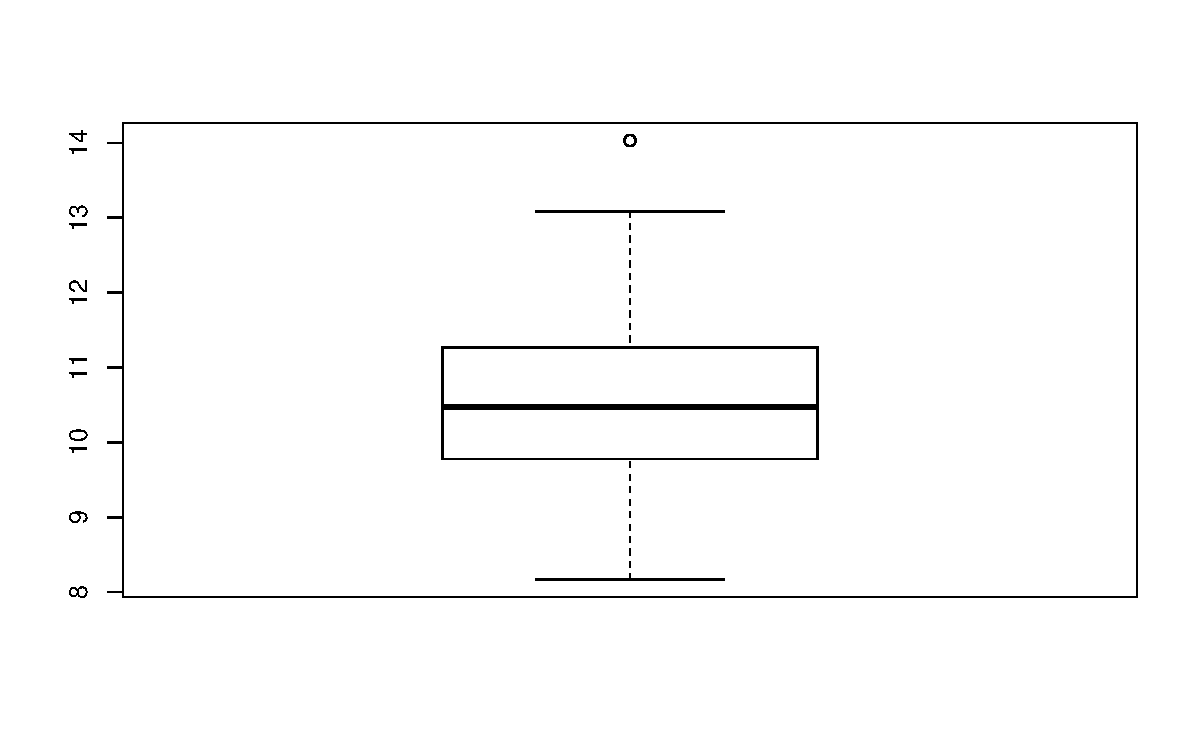
\includegraphics{01-preface_files/figure-latex/Figure8-1.pdf}
\caption{\label{fig:Figure8}Boxplot of 1.5 mile Run Times.}
\end{figure}

\begin{Shaded}
\begin{Highlighting}[]
\KeywordTok{boxplot}\NormalTok{(treadmill}\OperatorTok{$}\NormalTok{RunTime)}
\end{Highlighting}
\end{Shaded}

While the default boxplot is fine, it fails to provide good graphical
labels, especially on the y-axis. Additionally, there is no title on the
plot. The following code provides some enhancements to the plot by using
the \texttt{ylab} and \texttt{main} options in the call to
\texttt{boxplot}, with the results displayed in Figure
\ref{fig:Figure9}. When we add text to plots, it will be contained
within quotes and be assigned into the options \texttt{ylab} (for
y-axis) or \texttt{main} (for the title) here to put it into those
locations.



\begin{figure}
\centering
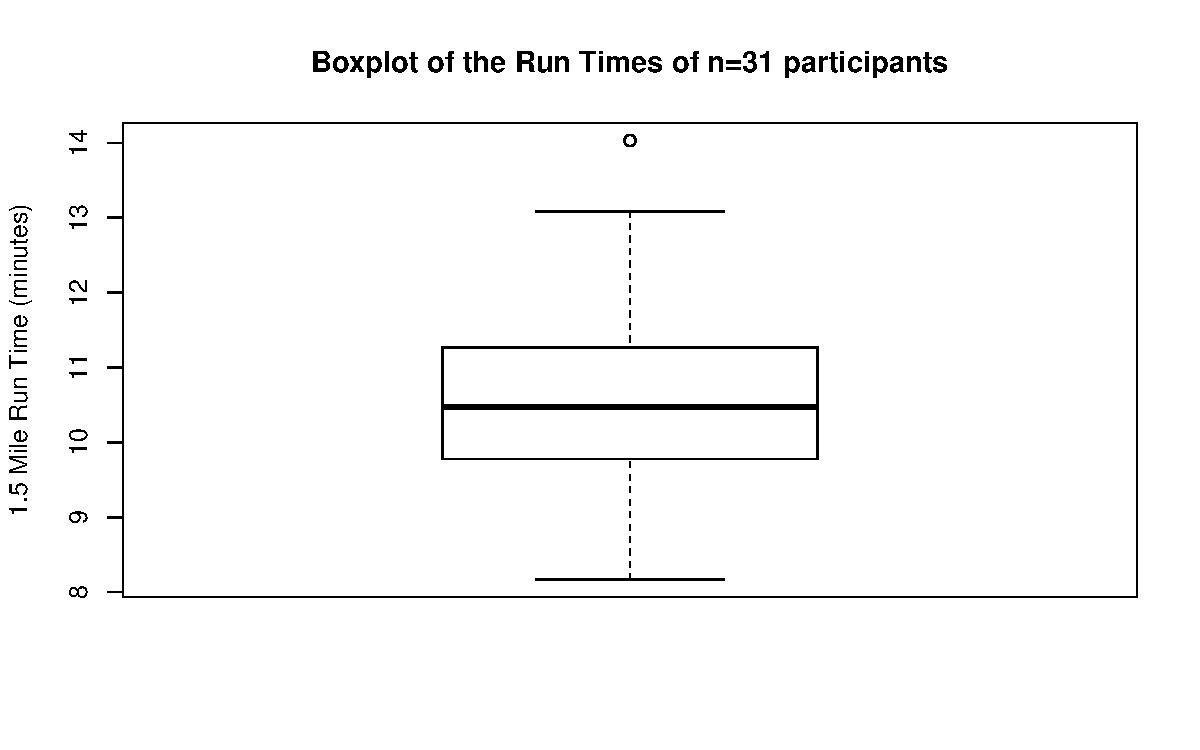
\includegraphics{01-preface_files/figure-latex/Figure9-1.pdf}
\caption{\label{fig:Figure9}Boxplot of Run Times with improved labels.}
\end{figure}

\begin{Shaded}
\begin{Highlighting}[]
\KeywordTok{boxplot}\NormalTok{(treadmill}\OperatorTok{$}\NormalTok{RunTime, }\DataTypeTok{ylab=}\StringTok{"1.5 Mile Run Time (minutes)"}\NormalTok{, }
        \DataTypeTok{main=}\StringTok{"Boxplot of the Run Times of n=31 participants"}\NormalTok{)}
\end{Highlighting}
\end{Shaded}

Throughout the book, we will often use extra options to make figures
that are easier for you to understand. There are often simpler versions
of the functions that will suffice but the extra work to get better
labeled figures is often worth it. I guess the point is that ``a picture
is worth a thousand words'' but in data visualization, that is only true
if the reader can understand what is being displayed. It is also
important to think about the quality of the information that is being
displayed, regardless of how pretty the graphic might be.

All the previous results were created by running the R code and then
``grabbing'' the results from either the console or by copying the
figure. There is another way to use RStudio where you can have it
compile the results (both output and figures) directly into a document
together with the code that generated it, using what is called RMarkdown
(\url{http://shiny.rstudio.com/articles/rmarkdown.html}). It adds some
additional setup complexity we want to avoid for now but is what we used
to do all the analyses that follow in the book. The main reason to
mention this is that you will see a change in formatting of the R code
and output from here forward as you will no longer see the command
prompt (``\textgreater{}'') with the code. The output will be flagged by
having two ``\#\#'''s before it. For example, the summary statistics for
the \emph{RunTime} variable from `\texttt{favstats} function would look
like:

\begin{Shaded}
\begin{Highlighting}[]
\KeywordTok{favstats}\NormalTok{(treadmill}\OperatorTok{$}\NormalTok{RunTime)}
\end{Highlighting}
\end{Shaded}

\begin{verbatim}
##   min   Q1 median    Q3   max     mean       sd  n missing
##  8.17 9.78  10.47 11.27 14.03 10.58613 1.387414 31       0
\end{verbatim}

Statisticians (and other scientists) are starting to use these methods
because they provide what is called ``Reproducible research''
\citep{Gandrud2015} where all the code and output it produced are
available in a single place. This allows different researchers to run
and verify results or the original researchers to revisit their earlier
work at a later date and recreate all their results. Scientific
publications are currently encouraging researchers to work in this way
and may someday require it. In this book, we focus on the R code and
show the results from running it, but you may want to consider exploring
these alternative options.

Finally, when you are done with your work and attempt to exit out of
RStudio, it will ask you to save your workspace. You do not need to do
this and would be better served not to do this. If you are in the
practice of saving your workspace, you will end up with tons of
data.frames that open each time you use it and it will be harder to find
and manage the ones you are currently working with. If you save your R
code via the script window, you can re-create any results by simply
re-running that code. If you find that you have lots of ``stuff'' in
your workspace, just run \texttt{rm(list\ =\ ls())}. It will delete all
the data sets from your workspace.

\section{Chapter summary}\label{chapter-summary}

This chapter covered getting R and RStudio downloaded and some basics of
working with R via RStudio. You should be able to read a data set into R
and run some basic functions, all done using the RStudio interface. If
you are struggling with this, you should seek additional help with these
technical issues so that you are ready for more complicated statistical
methods that are going to be encountered in the following chapters. For
most assignments, we will give you a seed of the basic R code that you
need and then you will modify it to work on your data set of interest.
As mentioned previously, the way everyone learns R is by starting with
some example code that does most of what you want to do and then you
modify it. If you can complete the Practice Problems that follow, you
are well on your way to learning to use R.

The statistical methods in this chapter were minimal and all should have
been review. They involved a quick reminder of summarizing the center,
spread, and shape of distributions using numerical summaries of the mean
and SD and/or the min, Q1, median, Q3, and max and the histogram and
boxplot as graphical summaries. We revisited the ideas of symmetry and
skew. But the main point was really to get a start on using R to provide
results you should be familiar with from your previous statistics
experience(s).

\section{Important R Code}\label{important-r-code}

To help you learn and use R, there is a section highlighting the most
important R code used near the end of each chapter. The dark text will
never change but the lighter (red) text will need to be customized to
your particular application. The sub-bullet for each function will
discuss the use of the function and pertinent options or packages
required. You can use this as a guide to finding the function names and
some hints about options that will help you to get the code to work or
you can revisit the worked examples using each of the functions.

\begin{itemize}
\item
  \textcolor{red}{FILENAME}\textless{}-
  read.csv(\textcolor{red}{"path to csv file/FILENAME.csv"})

  \begin{itemize}
  \tightlist
  \item
    Can be generated using ``Import Dataset'' button or by modifying
    this text.
  \end{itemize}
\item
  \textcolor{red}{DATASETNAME}\$\textcolor{red}{VARIABLENAME}

  \begin{itemize}
  \tightlist
  \item
    To access a particular variable in a data.frame called DATASETNAME,
    use a \$ and then the VARIABLENAME.
  \end{itemize}
\item
  head(\textcolor{red}{DATASETNAME})

  \begin{itemize}
  \tightlist
  \item
    Provides a list of the first few rows of the data set for all the
    variables in it.
  \end{itemize}
\item
  mean(\textcolor{red}{DATASETNAME}\$\textcolor{red}{VARIABLENAME})

  \begin{itemize}
  \tightlist
  \item
    Calculates the mean of the observations in a variable.
  \end{itemize}
\item
  sd(\textcolor{red}{DATASETNAME}\$\textcolor{red}{VARIABLENAME})

  \begin{itemize}
  \tightlist
  \item
    Calculates the SD of the observations in a variable.
  \end{itemize}
\item
  favstats(\textcolor{red}{DATASETNAME}\$\textcolor{red}{VARIABLENAME})

  \begin{itemize}
  \item
    Requires the \texttt{mosaic} package to be loaded
    (\texttt{require(mosaic}) after installing the package).
  \item
    Provides a suite of numerical summaries of the observations in a
    variable.
  \end{itemize}
\item
  hist(\textcolor{red}{DATASETNAME}\$\textcolor{red}{VARIABLENAME})

  \begin{itemize}
  \tightlist
  \item
    Makes a histogram.
  \end{itemize}
\item
  boxplot(\textcolor{red}{DATASETNAME}\$\textcolor{red}{VARIABLENAME})

  \begin{itemize}
  \tightlist
  \item
    Makes a boxplot.
  \end{itemize}
\end{itemize}

\section{Practice problems}\label{practice-problems}

In each chapter, the last section contains some questions for you to
complete to make sure you understood the material. You can download the
code to answer questions 0.1 to 0.5 below at
\url{http://www.math.montana.edu/courses/s217/documents/Ch0.Rmd}. But to
practice learning R, it would be most useful for you to try to
accomplish the requested tasks yourself and then only refer to the
provided R code if/when you struggle. These questions provide a great
venue to check your learning, often to see the methods applied to
another data set, and for something to discuss in study groups, with
your instructor, and/or at the Math Learning Center.

1.1. Read in the treadmill data set discussed above and find the mean
and SD of the Ages (\emph{Age} variable) and Body Weights
(\emph{BodyWeight} variable). In studies involving human subjects, it is
common to report a summary of characteristics of the subjects. Why does
this matter? Think about how your interpretation of any study of the
fitness of subjects would change if the mean age had been 20 years older
or 35 years younger.

1.2. How does knowing about the distribution of results for \emph{Age}
and \emph{BodyWeight} help you understand the results for the Run Times
discussed above?

1.3. The mean and SD are most useful as summary statistics only if the
distribution is relatively symmetric. Make a discuss the shape of the
distribution (is it skewed right, skewed left, approximately symmetric?;
are there outliers?). Approximately what range of ages does this study
pertain to?

1.4. The weight responses are in kilograms and you might prefer to see
them in pounds. The conversion is lbs=2.205\emph{kgs. Create a new
variable in the \texttt{treadmill} data.frame called }BWlb* using this
code:

\texttt{treadmill\$BWlb\ \textless{}-\ 2.205*treadmill\$BodyWeight}

and find the mean and SD of the new variable (\emph{BWlb}).

1.5. Make histograms and boxplots of the original \emph{BodyWeight} and
new \emph{BWlb} variables. Discuss aspects of the distributions that
changed and those that remained the same with the transformation from
kilograms to pounds.

\chapter{(R)e-Introduction to statistics}\label{chapter2}

The previous material served to get us started in R and to get a quick
review of same basic descriptive statistics. Now we will begin to engage
some new material and exploit the power of R to do some statistical
inference. Because inference is one of the hardest topics to master in
statistics, we will also review some basic terminology that is required
to move forward in learning more sophisticated statistical methods. To
keep this ``review'' as short as possible, we will not consider every
situation you learned in introductory statistics and instead focus
exclusively on the situation where we have a quantitative response
variable measured on two groups, adding a new graphic called a ``bean
plot'' to help us see the differences in the observations in the groups.

\section{Histograms, boxplots, and density curves}\label{section2-1}

Part of learning statistics is learning to correctly use the
terminology, some of which is used colloquially differently than it is
used in formal statistical settings. The most commonly ``misused'' term
is \textbf{\emph{data}}. In statistical parlance, we want to note the
plurality of data. Specifically, \textbf{\emph{datum}} is a single
measurement, possibly on multiple random variables, and so it is
appropriate to say that ``\textbf{a datum is\ldots{}}''. Once we move to
discussing data, we are now referring to more than one observation,
again on one, or possibly more than one, random variable, and so we need
to use ``\textbf{data are\ldots{}}'' when talking about our
observations. We want to distinguish our use of the term ``data'' from
its more colloquial\footnote{You will more typically hear ``data is''
  but that more often refers to information, sometimes even statistical
  summaries of data sets, than to observations collected as part of a
  study, suggesting the confusion of this term in the general public. We
  will explore a data set in Chapter 4 related to perceptions of this
  issue collected by researchers at \url{http://fivethirtyeight.com/}.}
usage that often involves treating it as singular. In a statistical
setting ``data'' refers to measurements of our cases or units. When we
summarize the results of a study (say providing the mean and SD), that
information is not ``data''. We used our data to generate that
information. Sometimes we also use the term ``data set'' to refer to all
our observations and this is a singular term to refer to the group of
observations and this makes it really easy to make mistakes on the usage
of this term.

It is also really important to note that \textbf{\emph{variables}} have
to vary -- if you measure the sex of your subjects but are only
measuring females, then you do not have a ``variable''. You may not know
if you have real variability in a ``variable'' until you explore the
results you obtained.

The last, but probably most important, aspect of data is the context of
the measurement. The ``who, what, when, and where'' of the collection of
the observations is critical to the sort of conclusions we can make
based on the results. The information on the study design provides
information required to assess the scope of inference of the study.
Generally, remember to think about the research questions the
researchers were trying to answer and whether their study actually would
answer those questions. There are no formulas to help us sort some of
these things out, just critical thinking about the context of the
measurements.

To make this concrete, consider the data collected from a study
\citep{Plaster1989} to investigate whether perceived physical
attractiveness had an impact on the sentences or perceived seriousness
of a crime that male jurors might give to female defendants. The
researchers showed the participants in the study (men who volunteered
from a prison) pictures of one of three young women. Each picture had
previously been decided to be either beautiful, average, or unattractive
by the researchers. Each ``juror'' was randomly assigned to one of three
levels of this factor (which is a categorical predictor or explanatory
variable) and then each rated their picture on a variety of traits such
as how warm or sincere the woman appeared. Finally, they were told the
women had committed a crime (also randomly assigned to either be told
she committed a burglary or a swindle) and were asked to rate the
seriousness of the crime and provide a suggested length of sentence. We
will bypass some aspects of their research and just focus on differences
in the sentence suggested among the three pictures. To get a sense of
these data, let's consider the first and last parts of the data set:



\begin{longtable}[]{@{}ccccccc@{}}
\caption{\label{tab:Table2-1} First 5 and last 6 rows of the Mock Jury data set.}\tabularnewline
\toprule
\begin{minipage}[b]{0.11\columnwidth}\centering\strut
Subject\strut
\end{minipage} & \begin{minipage}[b]{0.11\columnwidth}\centering\strut
Attr\strut
\end{minipage} & \begin{minipage}[b]{0.10\columnwidth}\centering\strut
Crime\strut
\end{minipage} & \begin{minipage}[b]{0.09\columnwidth}\centering\strut
Years\strut
\end{minipage} & \begin{minipage}[b]{0.11\columnwidth}\centering\strut
Serious\strut
\end{minipage} & \begin{minipage}[b]{0.16\columnwidth}\centering\strut
Independent\strut
\end{minipage} & \begin{minipage}[b]{0.10\columnwidth}\centering\strut
Sincere\strut
\end{minipage}\tabularnewline
\midrule
\endfirsthead
\toprule
\begin{minipage}[b]{0.11\columnwidth}\centering\strut
Subject\strut
\end{minipage} & \begin{minipage}[b]{0.11\columnwidth}\centering\strut
Attr\strut
\end{minipage} & \begin{minipage}[b]{0.10\columnwidth}\centering\strut
Crime\strut
\end{minipage} & \begin{minipage}[b]{0.09\columnwidth}\centering\strut
Years\strut
\end{minipage} & \begin{minipage}[b]{0.11\columnwidth}\centering\strut
Serious\strut
\end{minipage} & \begin{minipage}[b]{0.16\columnwidth}\centering\strut
Independent\strut
\end{minipage} & \begin{minipage}[b]{0.10\columnwidth}\centering\strut
Sincere\strut
\end{minipage}\tabularnewline
\midrule
\endhead
\begin{minipage}[t]{0.11\columnwidth}\centering\strut
1\strut
\end{minipage} & \begin{minipage}[t]{0.11\columnwidth}\centering\strut
Beautiful\strut
\end{minipage} & \begin{minipage}[t]{0.10\columnwidth}\centering\strut
Burglary\strut
\end{minipage} & \begin{minipage}[t]{0.09\columnwidth}\centering\strut
10\strut
\end{minipage} & \begin{minipage}[t]{0.11\columnwidth}\centering\strut
8\strut
\end{minipage} & \begin{minipage}[t]{0.16\columnwidth}\centering\strut
9\strut
\end{minipage} & \begin{minipage}[t]{0.10\columnwidth}\centering\strut
8\strut
\end{minipage}\tabularnewline
\begin{minipage}[t]{0.11\columnwidth}\centering\strut
2\strut
\end{minipage} & \begin{minipage}[t]{0.11\columnwidth}\centering\strut
Beautiful\strut
\end{minipage} & \begin{minipage}[t]{0.10\columnwidth}\centering\strut
Burglary\strut
\end{minipage} & \begin{minipage}[t]{0.09\columnwidth}\centering\strut
3\strut
\end{minipage} & \begin{minipage}[t]{0.11\columnwidth}\centering\strut
8\strut
\end{minipage} & \begin{minipage}[t]{0.16\columnwidth}\centering\strut
9\strut
\end{minipage} & \begin{minipage}[t]{0.10\columnwidth}\centering\strut
3\strut
\end{minipage}\tabularnewline
\begin{minipage}[t]{0.11\columnwidth}\centering\strut
3\strut
\end{minipage} & \begin{minipage}[t]{0.11\columnwidth}\centering\strut
Beautiful\strut
\end{minipage} & \begin{minipage}[t]{0.10\columnwidth}\centering\strut
Burglary\strut
\end{minipage} & \begin{minipage}[t]{0.09\columnwidth}\centering\strut
5\strut
\end{minipage} & \begin{minipage}[t]{0.11\columnwidth}\centering\strut
5\strut
\end{minipage} & \begin{minipage}[t]{0.16\columnwidth}\centering\strut
6\strut
\end{minipage} & \begin{minipage}[t]{0.10\columnwidth}\centering\strut
3\strut
\end{minipage}\tabularnewline
\begin{minipage}[t]{0.11\columnwidth}\centering\strut
4\strut
\end{minipage} & \begin{minipage}[t]{0.11\columnwidth}\centering\strut
Beautiful\strut
\end{minipage} & \begin{minipage}[t]{0.10\columnwidth}\centering\strut
Burglary\strut
\end{minipage} & \begin{minipage}[t]{0.09\columnwidth}\centering\strut
1\strut
\end{minipage} & \begin{minipage}[t]{0.11\columnwidth}\centering\strut
3\strut
\end{minipage} & \begin{minipage}[t]{0.16\columnwidth}\centering\strut
9\strut
\end{minipage} & \begin{minipage}[t]{0.10\columnwidth}\centering\strut
8\strut
\end{minipage}\tabularnewline
\begin{minipage}[t]{0.11\columnwidth}\centering\strut
5\strut
\end{minipage} & \begin{minipage}[t]{0.11\columnwidth}\centering\strut
Beautiful\strut
\end{minipage} & \begin{minipage}[t]{0.10\columnwidth}\centering\strut
Burglary\strut
\end{minipage} & \begin{minipage}[t]{0.09\columnwidth}\centering\strut
7\strut
\end{minipage} & \begin{minipage}[t]{0.11\columnwidth}\centering\strut
9\strut
\end{minipage} & \begin{minipage}[t]{0.16\columnwidth}\centering\strut
5\strut
\end{minipage} & \begin{minipage}[t]{0.10\columnwidth}\centering\strut
1\strut
\end{minipage}\tabularnewline
\begin{minipage}[t]{0.11\columnwidth}\centering\strut
\ldots{}\strut
\end{minipage} & \begin{minipage}[t]{0.11\columnwidth}\centering\strut
\ldots{}\strut
\end{minipage} & \begin{minipage}[t]{0.10\columnwidth}\centering\strut
\ldots{}\strut
\end{minipage} & \begin{minipage}[t]{0.09\columnwidth}\centering\strut
\ldots{}\strut
\end{minipage} & \begin{minipage}[t]{0.11\columnwidth}\centering\strut
\ldots{}\strut
\end{minipage} & \begin{minipage}[t]{0.16\columnwidth}\centering\strut
\ldots{}\strut
\end{minipage} & \begin{minipage}[t]{0.10\columnwidth}\centering\strut
\ldots{}\strut
\end{minipage}\tabularnewline
\begin{minipage}[t]{0.11\columnwidth}\centering\strut
108\strut
\end{minipage} & \begin{minipage}[t]{0.11\columnwidth}\centering\strut
Average\strut
\end{minipage} & \begin{minipage}[t]{0.10\columnwidth}\centering\strut
Swindle\strut
\end{minipage} & \begin{minipage}[t]{0.09\columnwidth}\centering\strut
3\strut
\end{minipage} & \begin{minipage}[t]{0.11\columnwidth}\centering\strut
3\strut
\end{minipage} & \begin{minipage}[t]{0.16\columnwidth}\centering\strut
5\strut
\end{minipage} & \begin{minipage}[t]{0.10\columnwidth}\centering\strut
4\strut
\end{minipage}\tabularnewline
\begin{minipage}[t]{0.11\columnwidth}\centering\strut
109\strut
\end{minipage} & \begin{minipage}[t]{0.11\columnwidth}\centering\strut
Average\strut
\end{minipage} & \begin{minipage}[t]{0.10\columnwidth}\centering\strut
Swindle\strut
\end{minipage} & \begin{minipage}[t]{0.09\columnwidth}\centering\strut
3\strut
\end{minipage} & \begin{minipage}[t]{0.11\columnwidth}\centering\strut
2\strut
\end{minipage} & \begin{minipage}[t]{0.16\columnwidth}\centering\strut
9\strut
\end{minipage} & \begin{minipage}[t]{0.10\columnwidth}\centering\strut
9\strut
\end{minipage}\tabularnewline
\begin{minipage}[t]{0.11\columnwidth}\centering\strut
110\strut
\end{minipage} & \begin{minipage}[t]{0.11\columnwidth}\centering\strut
Average\strut
\end{minipage} & \begin{minipage}[t]{0.10\columnwidth}\centering\strut
Swindle\strut
\end{minipage} & \begin{minipage}[t]{0.09\columnwidth}\centering\strut
2\strut
\end{minipage} & \begin{minipage}[t]{0.11\columnwidth}\centering\strut
1\strut
\end{minipage} & \begin{minipage}[t]{0.16\columnwidth}\centering\strut
8\strut
\end{minipage} & \begin{minipage}[t]{0.10\columnwidth}\centering\strut
8\strut
\end{minipage}\tabularnewline
\begin{minipage}[t]{0.11\columnwidth}\centering\strut
111\strut
\end{minipage} & \begin{minipage}[t]{0.11\columnwidth}\centering\strut
Average\strut
\end{minipage} & \begin{minipage}[t]{0.10\columnwidth}\centering\strut
Swindle\strut
\end{minipage} & \begin{minipage}[t]{0.09\columnwidth}\centering\strut
7\strut
\end{minipage} & \begin{minipage}[t]{0.11\columnwidth}\centering\strut
4\strut
\end{minipage} & \begin{minipage}[t]{0.16\columnwidth}\centering\strut
9\strut
\end{minipage} & \begin{minipage}[t]{0.10\columnwidth}\centering\strut
1\strut
\end{minipage}\tabularnewline
\begin{minipage}[t]{0.11\columnwidth}\centering\strut
112\strut
\end{minipage} & \begin{minipage}[t]{0.11\columnwidth}\centering\strut
Average\strut
\end{minipage} & \begin{minipage}[t]{0.10\columnwidth}\centering\strut
Swindle\strut
\end{minipage} & \begin{minipage}[t]{0.09\columnwidth}\centering\strut
6\strut
\end{minipage} & \begin{minipage}[t]{0.11\columnwidth}\centering\strut
3\strut
\end{minipage} & \begin{minipage}[t]{0.16\columnwidth}\centering\strut
5\strut
\end{minipage} & \begin{minipage}[t]{0.10\columnwidth}\centering\strut
2\strut
\end{minipage}\tabularnewline
\begin{minipage}[t]{0.11\columnwidth}\centering\strut
113\strut
\end{minipage} & \begin{minipage}[t]{0.11\columnwidth}\centering\strut
Average\strut
\end{minipage} & \begin{minipage}[t]{0.10\columnwidth}\centering\strut
Swindle\strut
\end{minipage} & \begin{minipage}[t]{0.09\columnwidth}\centering\strut
12\strut
\end{minipage} & \begin{minipage}[t]{0.11\columnwidth}\centering\strut
9\strut
\end{minipage} & \begin{minipage}[t]{0.16\columnwidth}\centering\strut
9\strut
\end{minipage} & \begin{minipage}[t]{0.10\columnwidth}\centering\strut
1\strut
\end{minipage}\tabularnewline
\begin{minipage}[t]{0.11\columnwidth}\centering\strut
114\strut
\end{minipage} & \begin{minipage}[t]{0.11\columnwidth}\centering\strut
Average\strut
\end{minipage} & \begin{minipage}[t]{0.10\columnwidth}\centering\strut
Swindle\strut
\end{minipage} & \begin{minipage}[t]{0.09\columnwidth}\centering\strut
8\strut
\end{minipage} & \begin{minipage}[t]{0.11\columnwidth}\centering\strut
8\strut
\end{minipage} & \begin{minipage}[t]{0.16\columnwidth}\centering\strut
1\strut
\end{minipage} & \begin{minipage}[t]{0.10\columnwidth}\centering\strut
5\strut
\end{minipage}\tabularnewline
\bottomrule
\end{longtable}

When working with data, we should always start with summarizing the
sample size. We will use \textbf{\emph{n}} for the number of subjects in
the sample and denote the population size (if available) with
\textbf{\emph{N}}. Here, the sample size is \textbf{\emph{n=114}}. In
this situation, we do not have a random sample from a population (these
were volunteers from the population of prisoners at the particular
prison) so we cannot make inferences to a larger group. But we can
assess whether there is a \textbf{\emph{causal effect}}\footnote{As
  noted previously, we reserve the term ``effect'' for situations where
  random assignment allows us to consider causality as the reason for
  the differences in the response variable among levels of the
  explanatory variable, but this is only the case if we find evidence
  against the null hypothesis of no difference in the groups.}: if
sufficient evidence is found to conclude that there is some difference
in the responses across the treated groups, we can attribute those
differences to the treatments applied, since the groups should be same
otherwise due to the pictures being randomly assigned to the ``jurors''.
The story of the data set -- that it was collected on prisoners --
becomes pretty important in thinking about the ramifications of any
results. Are male prisoners different from the population of college
males or all residents of a state such as Montana? If so, then we should
not assume that the detected differences, if detected, would also exist
in some other group of male subjects. The lack of a random sample makes
it impossible to assume that this set of prisoners might be like other
prisoners. So there are definite limitations to the inferences in the
following results. But it is still interesting to see if the pictures
caused a difference in the suggested mean sentences, even though the
inferences are limited to this group of prisoners. If this had been an
observational study (suppose that the prisoners could select one of the
three pictures), then we would have to avoid any of the ``causal''
language that we can consider here because the pictures were not
randomly assigned to the subjects. Without random assignment, the
explanatory variable of picture choice could be
\textbf{\emph{confounded}} with another characteristic of prisoners that
was related to which picture they selected and the rating they provided.
Confounding is not the only reason to avoid causal statements with
non-random assignment but the inability to separate the effect of other
variables (measured or unmeasured) from the differences we are observing
means that our inferences in these situations need to be carefully
stated.

Instead of loading this data set into R using the ``Import Dataset''
functionality, we can load an R package that contains the data, making
for easy access to this data set. The package called \texttt{heplots}
\citep{R-heplots} contains a data set called MockJury that contains the
results of the study. We also rely the R package called \texttt{mosaic}
\citep{R-mosaic} that was introduced previously. First (but only once),
you need to install both packages, which can be done either using the
Packages tab in the lower right panel of R-studio or using the
\texttt{install.packages} function with quotes around the package name:

\begin{Shaded}
\begin{Highlighting}[]
\OperatorTok{>}\StringTok{ }\NormalTok{install. }\KeywordTok{packages}\NormalTok{(}\StringTok{"heplots"}\NormalTok{)}
\end{Highlighting}
\end{Shaded}

After making sure that both packages are installed, we use the
\texttt{require} function around the package name (no quotes now!) to
load the package, something that you need to do any time you want to use
features of a package.

\begin{Shaded}
\begin{Highlighting}[]
\KeywordTok{require}\NormalTok{(heplots)}
\KeywordTok{require}\NormalTok{(mosaic)}
\end{Highlighting}
\end{Shaded}

There will be some results of the loading process that may discuss
loading other required packages. If the output says that it needs a
package that is unavailable, then follow the same process noted above to
install that package as well.

To load the data set that is available in an active package, we use the
\texttt{data} function.

\begin{Shaded}
\begin{Highlighting}[]
\KeywordTok{data}\NormalTok{(MockJury)}
\end{Highlighting}
\end{Shaded}

Now there will be a data.frame called \texttt{MockJury} available for us
to analyze and some information about it in the Environment tab. Again,
we can find out more about the data set in a couple of ways. First, we
can use the \texttt{View} function to provide a spreadsheet type of
display in the upper left panel. Second, we can use the \texttt{head}
and \texttt{tail} functions to print out the beginning and end of the
data set. Because there are so many variables, it may wrap around to
show all the columns.

\begin{Shaded}
\begin{Highlighting}[]
\KeywordTok{View}\NormalTok{(MockJury)}
\KeywordTok{head}\NormalTok{(MockJury)}
\end{Highlighting}
\end{Shaded}

\begin{verbatim}
##        Attr    Crime Years Serious exciting calm independent sincere warm
## 1 Beautiful Burglary    10       8        6    9           9       8    5
## 2 Beautiful Burglary     3       8        9    5           9       3    5
## 3 Beautiful Burglary     5       5        3    4           6       3    6
## 4 Beautiful Burglary     1       3        3    6           9       8    8
## 5 Beautiful Burglary     7       9        1    1           5       1    8
## 6 Beautiful Burglary     7       9        1    5           7       5    8
##   phyattr sociable kind intelligent strong sophisticated happy ownPA
## 1       9        9    9           6      9             9     5     9
## 2       9        9    4           9      5             5     5     7
## 3       7        4    2           4      5             4     5     5
## 4       9        9    9           9      9             9     9     9
## 5       8        9    4           7      9             9     8     7
## 6       8        9    5           8      9             9     9     9
\end{verbatim}

\begin{Shaded}
\begin{Highlighting}[]
\KeywordTok{tail}\NormalTok{(MockJury)}
\end{Highlighting}
\end{Shaded}

\begin{verbatim}
##        Attr   Crime Years Serious exciting calm independent sincere warm
## 109 Average Swindle     3       2        7    6           9       9    6
## 110 Average Swindle     2       1        8    8           8       8    8
## 111 Average Swindle     7       4        1    6           9       1    1
## 112 Average Swindle     6       3        5    3           5       2    4
## 113 Average Swindle    12       9        1    9           9       1    1
## 114 Average Swindle     8       8        1    9           1       5    1
##     phyattr sociable kind intelligent strong sophisticated happy ownPA
## 109       4        7    6           8      6             5     7     2
## 110       8        9    9           9      9             9     9     6
## 111       1        9    4           1      1             1     1     9
## 112       1        4    9           3      3             9     5     3
## 113       1        9    1           9      9             1     9     1
## 114       1        9    1           1      9             5     1     1
\end{verbatim}

When data sets are loaded from packages, there is often extra
documentation available about the data set which can be accessed using
the help function. In this case, it will bring up a screen with
information about the study and each variable that was measured.

\begin{Shaded}
\begin{Highlighting}[]
\KeywordTok{help}\NormalTok{(MockJury)}
\end{Highlighting}
\end{Shaded}

The help function is also useful with functions in R to help you
understand options and, at the bottom of the help, see examples of using
the function.

With many variables in a data set, it is often useful to get some quick
information about all of them; the \texttt{summary} function provides
useful information whether the variables are categorical or quantitative
and notes if any values were missing.

\begin{Shaded}
\begin{Highlighting}[]
\KeywordTok{summary}\NormalTok{(MockJury)}
\end{Highlighting}
\end{Shaded}

\begin{verbatim}
##            Attr         Crime        Years           Serious     
##  Beautiful   :39   Burglary:59   Min.   : 1.000   Min.   :1.000  
##  Average     :38   Swindle :55   1st Qu.: 2.000   1st Qu.:3.000  
##  Unattractive:37                 Median : 3.000   Median :5.000  
##                                  Mean   : 4.693   Mean   :5.018  
##                                  3rd Qu.: 7.000   3rd Qu.:6.750  
##                                  Max.   :15.000   Max.   :9.000  
##     exciting          calm        independent       sincere     
##  Min.   :1.000   Min.   :1.000   Min.   :1.000   Min.   :1.000  
##  1st Qu.:3.000   1st Qu.:4.250   1st Qu.:5.000   1st Qu.:3.000  
##  Median :5.000   Median :6.500   Median :6.500   Median :5.000  
##  Mean   :4.658   Mean   :5.982   Mean   :6.132   Mean   :4.789  
##  3rd Qu.:6.000   3rd Qu.:8.000   3rd Qu.:8.000   3rd Qu.:7.000  
##  Max.   :9.000   Max.   :9.000   Max.   :9.000   Max.   :9.000  
##       warm         phyattr        sociable          kind      
##  Min.   :1.00   Min.   :1.00   Min.   :1.000   Min.   :1.000  
##  1st Qu.:2.00   1st Qu.:2.00   1st Qu.:5.000   1st Qu.:3.000  
##  Median :5.00   Median :5.00   Median :7.000   Median :5.000  
##  Mean   :4.57   Mean   :4.93   Mean   :6.132   Mean   :4.728  
##  3rd Qu.:7.00   3rd Qu.:8.00   3rd Qu.:8.000   3rd Qu.:7.000  
##  Max.   :9.00   Max.   :9.00   Max.   :9.000   Max.   :9.000  
##   intelligent        strong      sophisticated       happy      
##  Min.   :1.000   Min.   :1.000   Min.   :1.000   Min.   :1.000  
##  1st Qu.:4.000   1st Qu.:4.000   1st Qu.:3.250   1st Qu.:3.000  
##  Median :7.000   Median :6.000   Median :5.000   Median :5.000  
##  Mean   :6.096   Mean   :5.649   Mean   :5.061   Mean   :5.061  
##  3rd Qu.:8.750   3rd Qu.:7.000   3rd Qu.:7.000   3rd Qu.:7.000  
##  Max.   :9.000   Max.   :9.000   Max.   :9.000   Max.   :9.000  
##      ownPA      
##  Min.   :1.000  
##  1st Qu.:5.000  
##  Median :6.000  
##  Mean   :6.377  
##  3rd Qu.:9.000  
##  Max.   :9.000
\end{verbatim}

If we take a few moments to explore the output we can discover some
useful aspects of the data set. The output is organized by variable,
providing summary information based on the type of variable, either
counts by category for categorical variables \texttt{Attr} and
\texttt{Crime} mean for quantitative variables. If present, you would
also get a count of missing values that are called ``NAs'' in R. For the
first variable, called \texttt{Attr} in the data.frame and that we might
we find counts of the number of subjects shown each picture: 37/114
viewed the ``Unattractive'' picture, 38 viewed ``Average'', and 39
viewed ``Beautiful''. We can also see that suggested prison sentences
(data.frame variable \texttt{Years} ) ranged from 1 year to 15 years
with a median of 3 years. It seems that all the other variables except
for \emph{Crime} (type of crime that they were told the pictured woman
committed) contained responses between 1 and 9 based on rating scales
from 1 = low to 9 = high.

To accompany the numerical summaries, histograms, and boxplots can
provide some initial information on the shape of the distribution of the
responses for the Figure \ref{fig:Figure2-1} contains the histogram and
boxplot of Years, ignoring any information on which picture the
``jurors'' were shown. The calls to the two plotting functions are
enhanced slightly to add better labels.



\begin{figure}
\centering
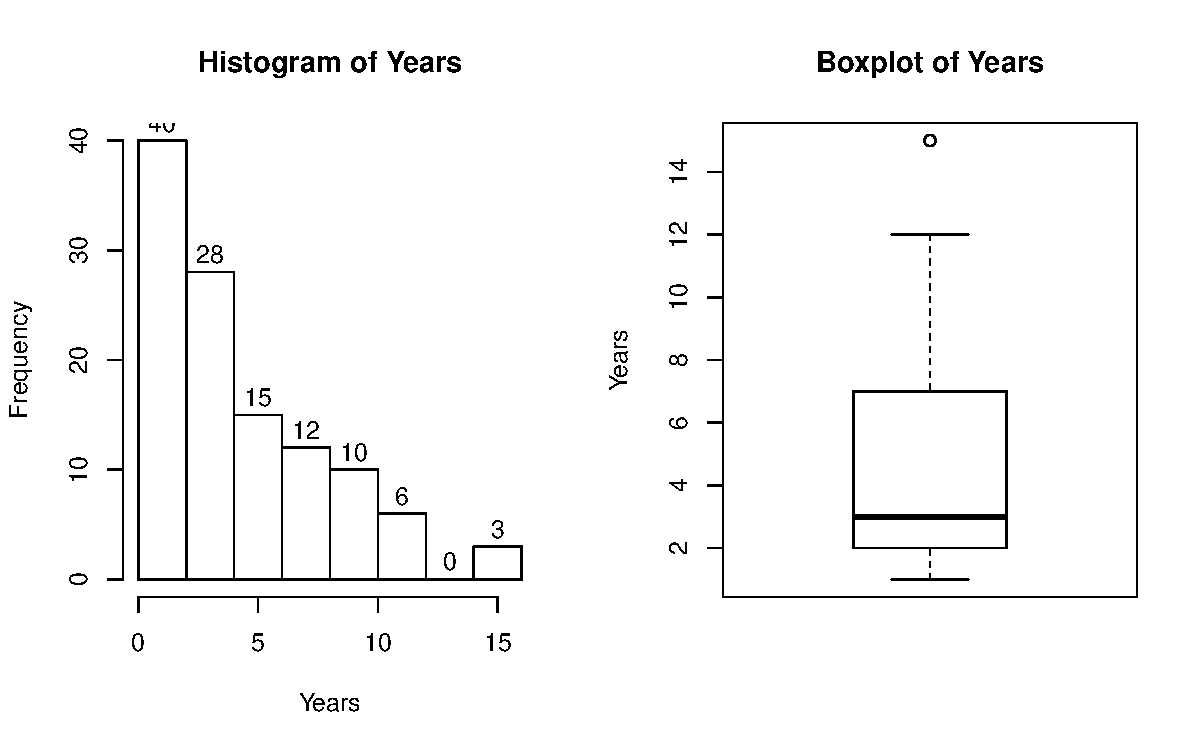
\includegraphics{02-reintroductionToStatistics_files/figure-latex/Figure2-1-1.pdf}
\caption{\label{fig:Figure2-1}Histogram and boxplot of suggested sentences in years.}
\end{figure}

\begin{Shaded}
\begin{Highlighting}[]
\KeywordTok{par}\NormalTok{(}\DataTypeTok{mfrow=}\KeywordTok{c}\NormalTok{(}\DecValTok{1}\NormalTok{,}\DecValTok{2}\NormalTok{))}
\KeywordTok{hist}\NormalTok{(MockJury}\OperatorTok{$}\NormalTok{Years, }\DataTypeTok{xlab=}\StringTok{"Years"}\NormalTok{, }\DataTypeTok{labels=}\NormalTok{T, }\DataTypeTok{main=}\StringTok{"Histogram of Years"}\NormalTok{)}
\KeywordTok{boxplot}\NormalTok{(MockJury}\OperatorTok{$}\NormalTok{Years, }\DataTypeTok{ylab=}\StringTok{"Years"}\NormalTok{, }\DataTypeTok{main=}\StringTok{"Boxplot of Years"}\NormalTok{)}
\end{Highlighting}
\end{Shaded}

The distribution appears to have a strong right skew with three
observations at 15 years flagged as potential outliers. You can only
tell that there are three observations and that they are at 15 by
looking at both plots -- the bar around 15 years in the histogram has a
count of three and the boxplot only shows a single point at 15 which is
actually three tied points at exactly 15 years plotted on top of each
other (we call this ``overplotting''). These three observations really
seem to be the upper edge of the overall pattern of a strongly right
skewed distribution, so even though they are flagged in the boxplot, we
likely would not want to remove them from our data set. In real data
sets, outliers are commonly encountered and the first step is to verify
that they were not errors in recording. The next step is to study their
impact on the statistical analyses performed, potentially considering
reporting results with and without the influential observation(s) in the
results. If the analysis is unaffected by the ``unusual'' observations,
then it matters little whether they are dropped or not. If they do
affect the results, then reporting both versions of results allows the
reader to judge the impacts for themselves. It is important to remember
that sometimes the outliers are the most interesting part of the data
set.

Often when statisticians think of distributions, we think of the smooth
underlying shape that led to the data set that is being displayed in the
histogram. Instead of binning up observations and making bars in the
histogram, we can estimate what is called a \textbf{\emph{density curve
}} as a smooth curve that represents the observed distribution of the
responses. Density curves can sometimes help us see features of the data
sets more clearly.

To understand the density curve, it is useful to initially see the
histogram and density curve together. The density curve is scaled so
that the total area\footnote{If you've taken calculus, you will know
  that the curve is being constructed so that the integral from
  \(-\infty\) to \(\infty\) is 1. If you don't know calculus, think of a
  rectangle with area of 1 based on its height and width. These cover
  the same area but the top of the region wiggles.} under the curve is
1. To make a comparable histogram, the y-axis needs to be scaled so that
the histogram is also on the ``density'' scale which makes the bar
heights required so that the proportion of the total data set in each
bar is represented by the area in each bar (remember that area is height
times width). So the height depends on the width of the bars and the
total area across all the bars has to be 1. In the \texttt{hist}
function, the \texttt{freq=F} to get density-scaled histogram bars. The
density curve is added to the histogram using the R code of
\texttt{lines(density())}, producing the result in Figure
\ref{fig:Figure2-2} with added modifications of options for \texttt{lwd}
(line width) and \texttt{col} (color) to make the plot more interesting.
You can see how the density curve somewhat matches the histogram bars
but deals with the bumps up and down and edges a little differently. We
can pick out the strong right skew using either display and will rarely
make both together.



\begin{Shaded}
\begin{Highlighting}[]
\KeywordTok{hist}\NormalTok{(MockJury}\OperatorTok{$}\NormalTok{Years,}\DataTypeTok{freq=}\NormalTok{F,}\DataTypeTok{xlab=}\StringTok{"Years"}\NormalTok{,}\DataTypeTok{main=}\StringTok{"Histogram of Years"}\NormalTok{)}
\KeywordTok{lines}\NormalTok{(}\KeywordTok{density}\NormalTok{(MockJury}\OperatorTok{$}\NormalTok{Years),}\DataTypeTok{lwd=}\DecValTok{3}\NormalTok{,}\DataTypeTok{col=}\StringTok{"red"}\NormalTok{)}
\end{Highlighting}
\end{Shaded}

\begin{figure}
\centering
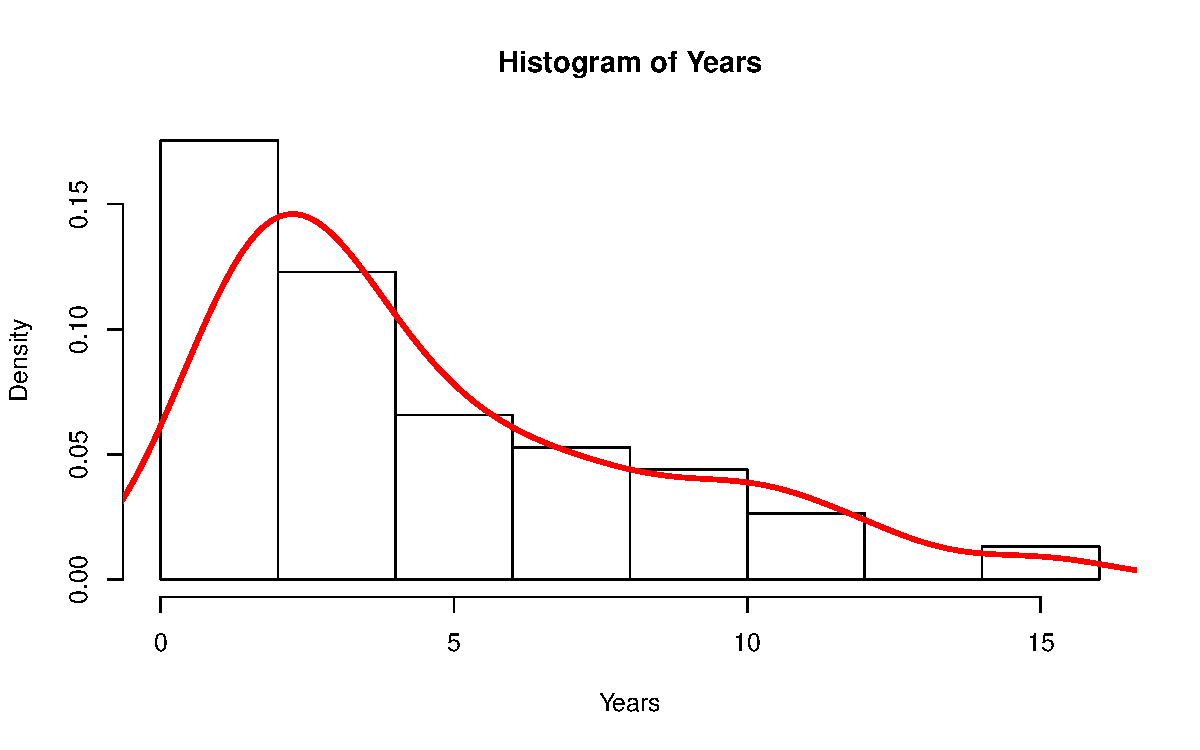
\includegraphics{02-reintroductionToStatistics_files/figure-latex/Figure2-2-1.pdf}
\caption{\label{fig:Figure2-2}Histogram and density curve of Years data.}
\end{figure}

Histograms can be sensitive to the choice of the number of bars and even
the cut-offs used to define the bins for a given number of bars. Small
changes in the definition of cut-offs for the bins can have noticeable
impacts on the shapes observed but this does not impact density curves.
We are not going to tinker with the default choices for bars in
histogram as they are reasonably selected, but we can add information on
the original observations being included in each bar to better
understand the choices that \texttt{hist} is making. In the previous
display, we can add what is called a \textbf{\emph{rug}} to the plot,
were a tick mark is made on the x-axis for each observation. Because the
responses were provided as whole years (1, 2, 3, \ldots{}, 15), we need
to use a graphical technique called \textbf{\emph{jittering}} to add a
little noise\footnote{Jittering typically involves adding random
  variability to each observation that is uniformly distributed in a
  range determined based on the spacing of the function, the results
  will change. For more details, type \texttt{help(jitter)} in R.} to
each observation so all the observations at each year value do not plot
as a single line. In Figure \ref{fig:Figure2-3}, the added tick marks on
the x-axis show the approximate locations of the original observations.
We can see how there are 3 observations at 15 (all were 15 and the noise
added makes it possible to see them all). The limitations of the
histogram arise around the 10 year sentence area where there are many
responses at 10 years and just one at both 9 and 11 years, but the
histogram bars sort of miss this that aspect of the data set. The
density curve did show a small bump at 10 years. Density curves are,
however, not perfect and this one shows area for sentences less than 0
years which is not possible here.




\begin{Shaded}
\begin{Highlighting}[]
\KeywordTok{hist}\NormalTok{(MockJury}\OperatorTok{$}\NormalTok{Years, }\DataTypeTok{freq=}\NormalTok{F, }\DataTypeTok{xlab=}\StringTok{"Years"}\NormalTok{,}
     \DataTypeTok{main=}\StringTok{"Histogram of Years with density curve and rug"}\NormalTok{)}
\KeywordTok{lines}\NormalTok{(}\KeywordTok{density}\NormalTok{(MockJury}\OperatorTok{$}\NormalTok{Years),}\DataTypeTok{lwd=}\DecValTok{3}\NormalTok{,}\DataTypeTok{col=}\StringTok{"red"}\NormalTok{)}
\KeywordTok{rug}\NormalTok{(}\KeywordTok{jitter}\NormalTok{(MockJury}\OperatorTok{$}\NormalTok{Years),}\DataTypeTok{col=}\StringTok{"blue"}\NormalTok{,}\DataTypeTok{lwd=}\DecValTok{2}\NormalTok{)}
\end{Highlighting}
\end{Shaded}

\begin{figure}
\centering
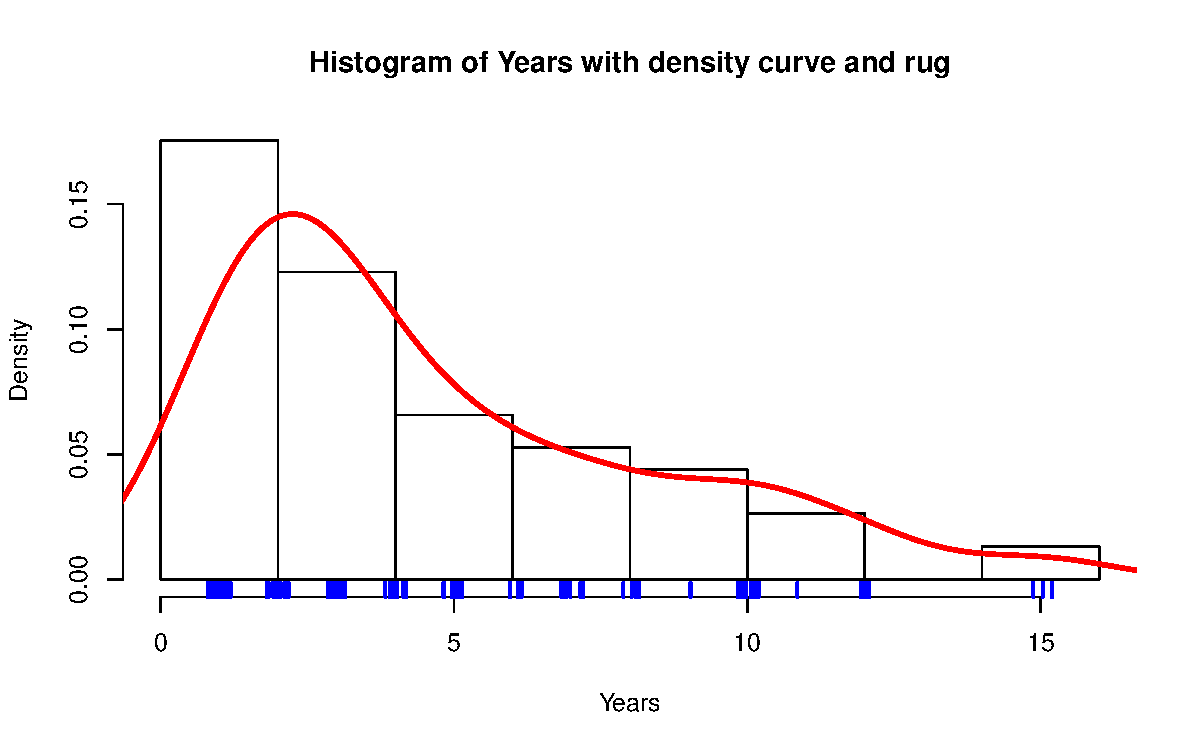
\includegraphics{02-reintroductionToStatistics_files/figure-latex/Figure2-3-1.pdf}
\caption{\label{fig:Figure2-3}Histogram with density curve and rug plot of the jittered
responses.}
\end{figure}

The graphical tools we've just discussed are going to help us move to
comparing the distribution of responses across more than one group. We
will have two displays that will help us make these comparisons. The
simplest is \emph{the \textbf{side-by-side boxplot}}, where a boxplot is
displayed for each group of interest using the same y-axis scaling. In
R, we can use its \textbf{\emph{formula}} notation to see if the
response (\texttt{Years}) differs based on the group (\texttt{Attr}) by
using something like \texttt{Y\textasciitilde{}X} or, here,
\texttt{Years\textasciitilde{}Attr}. We also need to tell R where to
find the variables -- use the last option in the command,
\texttt{data=DATASETNAME} , to inform R of the data.frame to look in to
find the variables. In this example, \texttt{data=MockJury}. We will use
the formula and \texttt{data=...} options in almost every function we
use from here forward. Figure \ref{fig:Figure2-4} contains the
side-by-side boxplots showing right skew for all the groups, slightly
higher median and more variability for the \emph{Unattractive} group
along with some potential outliers indicated in two of the three groups.



\begin{figure}
\centering
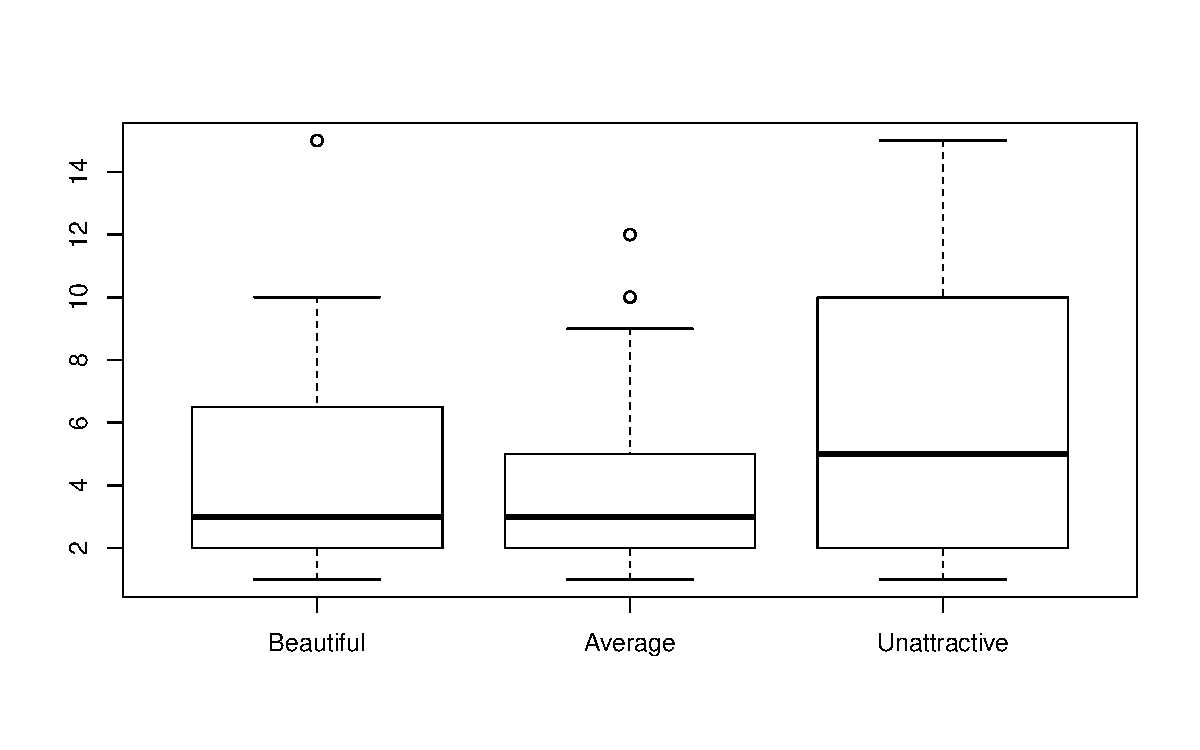
\includegraphics{02-reintroductionToStatistics_files/figure-latex/Figure2-4-1.pdf}
\caption{\label{fig:Figure2-4}Side-by-side boxplot of Years based on picture groups.}
\end{figure}

\begin{Shaded}
\begin{Highlighting}[]
\KeywordTok{boxplot}\NormalTok{(Years}\OperatorTok{~}\NormalTok{Attr,}\DataTypeTok{data=}\NormalTok{MockJury)}
\end{Highlighting}
\end{Shaded}

The ``\textasciitilde{}'' (which is read as the \emph{tilde} symbol,
which you can find in the upper left corner of your keyboard) notation
will be used in two ways this semester. The formula use in R employed
previously declares that the response variable here is \emph{Years} and
the explanatory variable is \emph{Attr}. The other use for
``\textasciitilde{}'' is as shorthand for ``is distributed as'' and is
used in the context of \texttt{Y\textasciitilde{}N(0,1)}, which
translates (in statistics) to defining the random variable \emph{Y} as
following a Normal distribution\footnote{Remember the bell-shaped curve
  you encountered in introductory statistics? If not, you can see some
  at \url{https://en.wikipedia.org/wiki/Normal_distribution}} with mean
0 and standard deviation of 1. In the current situation, we could ask
whether the \texttt{Years} variable seems like it may follow a normal
distribution, in other words, is
\emph{Years}\texttt{\textasciitilde{}N(0,1)}? Since the responses are
right skewed with some groups having outliers, it is not reasonable to
assume that the \emph{Years} variable for any of the three groups may
follow a Normal distribution (more later on the issues this creates!).
Remember that \(\mu\) and \(\sigma\) are parameters where \(\mu\)
(``mu'') is our standard symbol for the \textbf{\emph{population mean}}
and that \(\sigma\) (``sigma'') is the symbol of the
\textbf{\emph{population standard deviation}}.

\section{Beanplots}\label{section2-2}

The other graphical display for comparing multiple groups we will use is
a newer display called a \textbf{\emph{beanplot}} \citep{Kampstra2008}.
Figure \ref{fig:Figure2-5} shows an example of a beanplot that provides
a side-by-side display that contains the density curves, the original
observations that generated the density curve in a (jittered) rug-plot,
the mean of each group, and the overall mean of the entire data set. For
each group, the density curves are mirrored to aid in visual assessment
of the shape of the distribution, which makes a ``bean'' in some cases.
This mirroring also creates a shape that resembles a violin with skewed
distributions so this display has also been called a ``violin plot''.
The innovation in the beanplot is to add bold horizontal lines at the
mean for each group. It also adds a lighter dashed line for the overall
mean. All together this plot shows us information on the center (mean),
spread, and shape of the distributions of the responses. Our inferences
typically focus on the means of the groups and this plot allows us to
compare those across the groups while gaining information on the shapes
of the distributions of responses in each group.

To use the \texttt{beanplot} function we need to install and load the
\texttt{beanplot} package \citep{R-beanplot}. The function works like
the boxplot used previously except that options for \texttt{log},
\texttt{col}, and \texttt{method} need to be specified. Use
these\footnote{Well, you can use other colors (try ``lightblue'' for
  example), but I think bisque looks nice in these plots.} options for
any beanplots you make: \texttt{log="",\ col="bisque",\ method="jitter"}




\begin{figure}
\centering
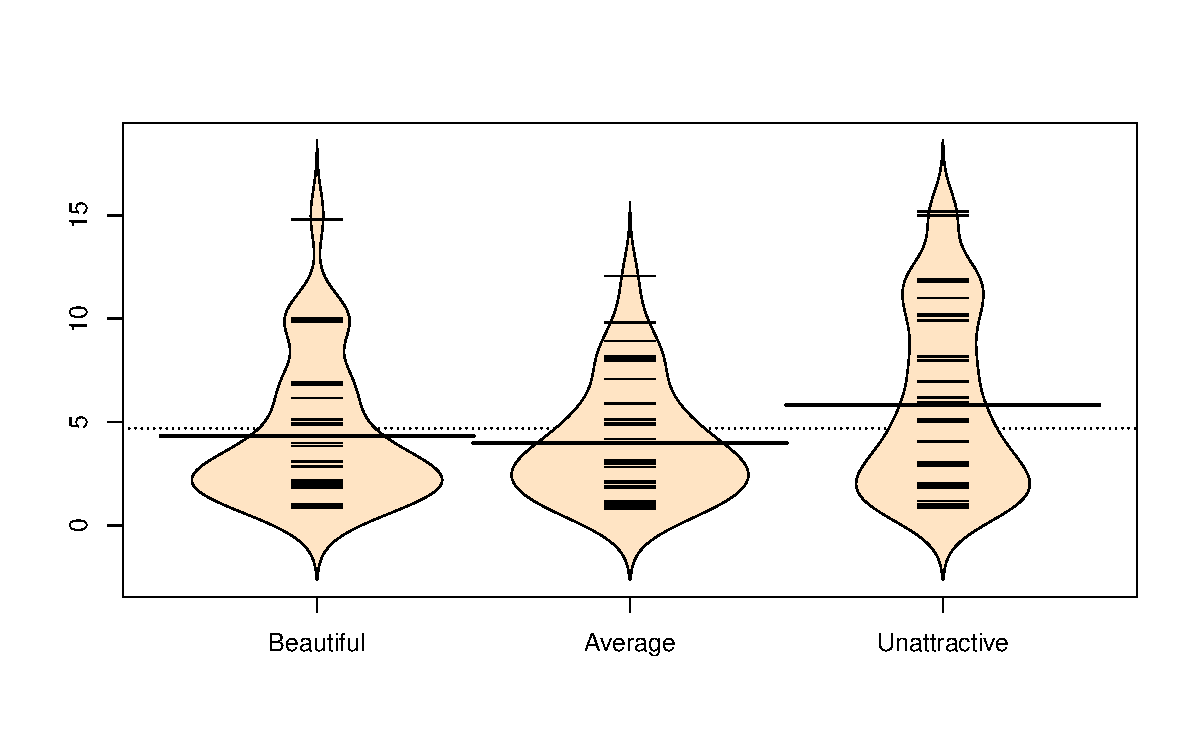
\includegraphics{02-reintroductionToStatistics_files/figure-latex/Figure2-5-1.pdf}
\caption{\label{fig:Figure2-5}Beanplot of Years by picture group. Long, bold lines
correspond to mean of each group.}
\end{figure}

\begin{Shaded}
\begin{Highlighting}[]
\KeywordTok{require}\NormalTok{(beanplot)}
\KeywordTok{beanplot}\NormalTok{(Years}\OperatorTok{~}\NormalTok{Attr,}\DataTypeTok{data=}\NormalTok{MockJury,}\DataTypeTok{log=}\StringTok{""}\NormalTok{,}\DataTypeTok{col=}\StringTok{"bisque"}\NormalTok{,}\DataTypeTok{method=}\StringTok{"jitter"}\NormalTok{)}
\end{Highlighting}
\end{Shaded}

Figure \ref{fig:Figure2-5} reinforces the strong right skews that were
also detected in the boxplots previously. The three large sentences of
15 years can now be clearly identified, with one in the \emph{Beautiful}
group and two in the \emph{Unattractive} group. The \emph{Unattractive}
group seems to have more high observations than the other groups even
though the \emph{Beautiful} group had the largest number of observations
around 10years. The mean sentence was highest for the
\emph{Unattractive} group and the difference in the means between
\emph{Beautiful} and \emph{Average} was small.

In this example, it appears that the mean for \emph{Unattractive} is
larger than the other two groups. But is this difference real? We will
never know the answer to that question, but we can assess how likely we
are to have seen a result as extreme or more extreme than our result,
assuming that there is no difference in the means of the groups. And if
the observed result is (extremely) unlikely to occur, then we can reject
the hypothesis that the groups have the same mean and conclude that
there is evidence of a real difference. To start exploring whether there
are differences in the means, we need to have numerical values to
compare. We can get means and standard deviations by groups easily using
the same formula notation with the \texttt{mean} and \texttt{sd}
functions if the \texttt{mosaic} package is loaded.

\begin{Shaded}
\begin{Highlighting}[]
\KeywordTok{mean}\NormalTok{(Years }\OperatorTok{~}\StringTok{ }\NormalTok{Attr, }\DataTypeTok{data =}\NormalTok{ MockJury)}
\end{Highlighting}
\end{Shaded}

\begin{verbatim}
##    Beautiful      Average Unattractive 
##     4.333333     3.973684     5.810811
\end{verbatim}

\begin{Shaded}
\begin{Highlighting}[]
\KeywordTok{sd}\NormalTok{(Years }\OperatorTok{~}\StringTok{ }\NormalTok{Attr, }\DataTypeTok{data =}\NormalTok{ MockJury)}
\end{Highlighting}
\end{Shaded}

\begin{verbatim}
##    Beautiful      Average Unattractive 
##     3.405362     2.823519     4.364235
\end{verbatim}

We can also use the \texttt{favstats} function to get those summaries
and others.

\begin{Shaded}
\begin{Highlighting}[]
\KeywordTok{favstats}\NormalTok{(Years }\OperatorTok{~}\StringTok{ }\NormalTok{Attr, }\DataTypeTok{data =}\NormalTok{ MockJury)}
\end{Highlighting}
\end{Shaded}

\begin{verbatim}
##           Attr min Q1 median   Q3 max     mean       sd  n missing
## 1    Beautiful   1  2      3  6.5  15 4.333333 3.405362 39       0
## 2      Average   1  2      3  5.0  12 3.973684 2.823519 38       0
## 3 Unattractive   1  2      5 10.0  15 5.810811 4.364235 37       0
\end{verbatim}

Based on these results, we can see that there is an estimated difference
of almost 2 years in the mean sentence between \emph{Average} and
\emph{Unattractive} groups. Because there are three groups being
compared in this study, we will have to wait until Chapter 3 and the
One-Way ANOVA test to fully assess evidence related to some difference
among the three groups. For now, we are going to focus on comparing the
mean \emph{Years} between \emph{Average} and \emph{Unattractive} groups
-- which is a \textbf{\emph{2 independent sample mean}} situation and
something you should have seen before. Remember that the ``independent''
sample part of this refers to observations that are independently
observed for the two groups as opposed to the paired sample situation
that you may have explored where one observation from the first group is
related to an observation in the second group (repeated measures on the
same person or the famous ``twin'' studies with one twin assigned to
each group).

Here we are going to use the ``simple'' two independent group scenario
to review some basic statistical concepts and connect two different
frameworks for conducting statistical inference: randomization and
parametric inference techniques. \textbf{\emph{Parametric}} statistical
methods involve making assumptions about the distribution of the
responses and obtaining confidence intervals and/or p-values using a
\emph{named} distribution (like the z or \(t\)-distributions). Typically
these results are generated using formulas and looking up areas under
curves or cutoffs using a table or a computer.
\textbf{\emph{Randomization}}-based statistical methods use a computer
to shuffle, sample, or simulate observations in ways that allow you to
obtain distributions of possible results to find areas and cutoffs
without resorting to using tables and named distributions. Randomization
methods are what are called \textbf{\emph{nonparametric}} methods that
often make fewer assumptions (they are \textbf{\emph{not free of
assumptions}}!) and so can handle a larger set of problems more easily
than parametric methods. When the assumptions involved in the parametric
procedures are met by a data set, the randomization methods often
provide very similar results to those provided by the parametric
techniques. To be a more sophisticated statistical consumer, it is
useful to have some knowledge of both of these approaches to statistical
inference and the fact that they can provide similar results might
deepen your understanding of both approaches.

We will start with comparing the \emph{Average} and \emph{Unattractive}
groups to compare these two ways of doing inference. We could remove the
\emph{Beautiful} group observations in a spreadsheet program and read
that new data set back into R, but it is actually pretty easy to use R
to do data management once the data set is loaded. To remove the
observations that came from the \emph{Beautiful} group, we are going to
generate a new variable that we will call \texttt{NotBeautiful} that is
true when observations came from another group (\emph{Average} or
\emph{Unattractive}) and false for observations from the
\emph{Beautiful} group. To do this, we will apply the \textbf{\emph{not
equal}} logical function (\texttt{!=} ) to the variable \texttt{Attr},
inquiring whether it was different from the \texttt{"Beautiful"} level.
You can see the content of the new variable in the output:

\begin{Shaded}
\begin{Highlighting}[]
\NormalTok{MockJury}\OperatorTok{$}\NormalTok{NotBeautiful <-}\StringTok{ }\NormalTok{MockJury}\OperatorTok{$}\NormalTok{Attr }\OperatorTok{!=}\StringTok{ "Beautiful"}
\NormalTok{MockJury}\OperatorTok{$}\NormalTok{NotBeautiful}
\end{Highlighting}
\end{Shaded}

\begin{verbatim}
##   [1] FALSE FALSE FALSE FALSE FALSE FALSE FALSE FALSE FALSE FALSE FALSE
##  [12] FALSE FALSE FALSE FALSE FALSE FALSE FALSE FALSE FALSE FALSE  TRUE
##  [23]  TRUE  TRUE  TRUE  TRUE  TRUE  TRUE  TRUE  TRUE  TRUE  TRUE  TRUE
##  [34]  TRUE  TRUE  TRUE  TRUE  TRUE  TRUE  TRUE  TRUE  TRUE  TRUE  TRUE
##  [45]  TRUE  TRUE  TRUE  TRUE  TRUE  TRUE  TRUE  TRUE  TRUE  TRUE  TRUE
##  [56]  TRUE  TRUE  TRUE  TRUE  TRUE  TRUE  TRUE  TRUE  TRUE  TRUE  TRUE
##  [67]  TRUE  TRUE  TRUE  TRUE  TRUE  TRUE  TRUE  TRUE  TRUE  TRUE FALSE
##  [78] FALSE FALSE FALSE FALSE FALSE FALSE FALSE FALSE FALSE FALSE FALSE
##  [89] FALSE FALSE FALSE FALSE FALSE FALSE  TRUE  TRUE  TRUE  TRUE  TRUE
## [100]  TRUE  TRUE  TRUE  TRUE  TRUE  TRUE  TRUE  TRUE  TRUE  TRUE  TRUE
## [111]  TRUE  TRUE  TRUE  TRUE
\end{verbatim}

This new variable is only FALSE for the \emph{Beautiful} responses as we
can see if we compare some of the results from the original and new
variable:

\begin{Shaded}
\begin{Highlighting}[]
\KeywordTok{head}\NormalTok{(}\KeywordTok{data.frame}\NormalTok{(MockJury}\OperatorTok{$}\NormalTok{Attr, MockJury}\OperatorTok{$}\NormalTok{NotBeautiful))}
\end{Highlighting}
\end{Shaded}

\begin{verbatim}
##   MockJury.Attr MockJury.NotBeautiful
## 1     Beautiful                 FALSE
## 2     Beautiful                 FALSE
## 3     Beautiful                 FALSE
## 4     Beautiful                 FALSE
## 5     Beautiful                 FALSE
## 6     Beautiful                 FALSE
\end{verbatim}

\newpage

\begin{Shaded}
\begin{Highlighting}[]
\KeywordTok{tail}\NormalTok{(}\KeywordTok{data.frame}\NormalTok{(MockJury}\OperatorTok{$}\NormalTok{Attr, MockJury}\OperatorTok{$}\NormalTok{NotBeautiful))}
\end{Highlighting}
\end{Shaded}

\begin{verbatim}
##     MockJury.Attr MockJury.NotBeautiful
## 109       Average                  TRUE
## 110       Average                  TRUE
## 111       Average                  TRUE
## 112       Average                  TRUE
## 113       Average                  TRUE
## 114       Average                  TRUE
\end{verbatim}

To get rid of one of the groups, we need to learn a little bit about
data management in R. \textbf{\emph{Brackets}} \texttt{({[},\ {]})} are
used to modify the rows or columns in a data.frame with entries before
the comma operating on rows and entries after the comma on the columns.
For example, if you want to see the results for the 5\(^{th}\) subject,
you can reference the 5\(^{th}\) row of the data.frame using
\texttt{{[}5,\ {]}} after the data.frame name:

\begin{Shaded}
\begin{Highlighting}[]
\NormalTok{MockJury[}\DecValTok{5}\NormalTok{,]}
\end{Highlighting}
\end{Shaded}

\begin{verbatim}
##        Attr    Crime Years Serious exciting calm independent sincere warm
## 5 Beautiful Burglary     7       9        1    1           5       1    8
##   phyattr sociable kind intelligent strong sophisticated happy ownPA
## 5       8        9    4           7      9             9     8     7
##   NotBeautiful
## 5        FALSE
\end{verbatim}

We could just extract the \emph{Years} response for the 5\(^{th}\)
subject by incorporating information on the row and column of interest
(\texttt{Years} is the 3\(^{rd}\) column):

\begin{Shaded}
\begin{Highlighting}[]
\NormalTok{MockJury[}\DecValTok{5}\NormalTok{,}\DecValTok{3}\NormalTok{]}
\end{Highlighting}
\end{Shaded}

\begin{verbatim}
## [1] 7
\end{verbatim}

In R, we can use logical vectors to keep any rows of the data.frame
where the variable is true and drop any rows where it is false by
placing the logical variable in the first element of the brackets. The
reduced version of the data set should be saved with a different name
such as \texttt{MockJury2} that is used here to reduce the chances of
confusing it with the previous full data set:

\begin{Shaded}
\begin{Highlighting}[]
\NormalTok{MockJury2 <-}\StringTok{ }\NormalTok{MockJury[MockJury}\OperatorTok{$}\NormalTok{NotBeautiful,]}
\end{Highlighting}
\end{Shaded}

You will always want to check that the correct observations were dropped
either using \texttt{View(MockJury2)} or by doing a quick summary of the
\texttt{Attr} variable in the new data.frame.

\begin{Shaded}
\begin{Highlighting}[]
\KeywordTok{summary}\NormalTok{(MockJury2}\OperatorTok{$}\NormalTok{Attr)}
\end{Highlighting}
\end{Shaded}

\begin{verbatim}
##    Beautiful      Average Unattractive 
##            0           38           37
\end{verbatim}

It ends up that R remembers the \emph{Beautiful} category even though
there are 0 observations in it now and that can cause us some problems.
When we remove a group of observations, we sometimes need to clean up
categorical variables to just reflect the categories that are present.
The \texttt{factor} function creates categorical variables based on the
levels of the variables that are observed and is useful to run here to
clean up \texttt{Attr}.

\begin{Shaded}
\begin{Highlighting}[]
\NormalTok{MockJury2}\OperatorTok{$}\NormalTok{Attr <-}\StringTok{ }\KeywordTok{factor}\NormalTok{(MockJury2}\OperatorTok{$}\NormalTok{Attr) }
\KeywordTok{summary}\NormalTok{(MockJury2}\OperatorTok{$}\NormalTok{Attr)}
\end{Highlighting}
\end{Shaded}

\begin{verbatim}
##      Average Unattractive 
##           38           37
\end{verbatim}

Now if we remake the boxplots and beanplots, they only contain results
for the two groups of interest here as seen in Figure
\ref{fig:Figure2-6}.




\begin{figure}
\centering
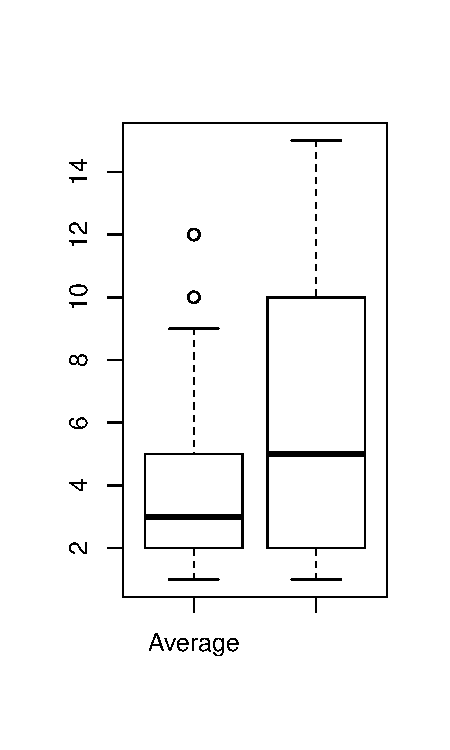
\includegraphics{02-reintroductionToStatistics_files/figure-latex/Figure2-6-1.pdf}
\caption{\label{fig:Figure2-6}Boxplot and beanplot of the Years responses on the reduced
data set.}
\end{figure}

\begin{Shaded}
\begin{Highlighting}[]
\KeywordTok{par}\NormalTok{(}\DataTypeTok{mfrow=}\KeywordTok{c}\NormalTok{(}\DecValTok{1}\NormalTok{,}\DecValTok{2}\NormalTok{))}
\KeywordTok{boxplot}\NormalTok{(Years }\OperatorTok{~}\StringTok{ }\NormalTok{Attr,}\DataTypeTok{data=}\NormalTok{MockJury2) }
\KeywordTok{beanplot}\NormalTok{(Years }\OperatorTok{~}\StringTok{ }\NormalTok{Attr,}\DataTypeTok{data=}\NormalTok{MockJury2,}\DataTypeTok{log=}\StringTok{""}\NormalTok{,}\DataTypeTok{col=}\StringTok{"bisque"}\NormalTok{,}\DataTypeTok{method=}\StringTok{"jitter"}\NormalTok{)}
\end{Highlighting}
\end{Shaded}

The two-sample mean techniques you learned in your previous course all
start with comparing the means the two groups. We can obtain the two
means using the \texttt{mean} function or directly obtain the difference
in the means using the \texttt{diffmean} function (both require the
\texttt{mosaic} package). The \texttt{diffmean} function provides
\(\bar{x}_{Unattractive} - \bar{x}_{Average}\) where \(\bar{x}\) (read
as ``x-bar'') is the sample mean of observations in the subscripted
group. Note that there are two directions that you could compare the
means and this function chooses to take the mean from the second group
name \emph{alphabetically} and subtract the mean from the first
alphabetical group name. It is always good to check the direction of
this calculation as having a difference of \(-1.84\) years versus
\(1.84\) years could be important.

\begin{Shaded}
\begin{Highlighting}[]
\KeywordTok{mean}\NormalTok{(Years }\OperatorTok{~}\StringTok{ }\NormalTok{Attr, }\DataTypeTok{data=}\NormalTok{MockJury2)}
\end{Highlighting}
\end{Shaded}

\begin{verbatim}
##      Average Unattractive 
##     3.973684     5.810811
\end{verbatim}

\begin{Shaded}
\begin{Highlighting}[]
\KeywordTok{diffmean}\NormalTok{(Years }\OperatorTok{~}\StringTok{ }\NormalTok{Attr, }\DataTypeTok{data=}\NormalTok{MockJury2)}
\end{Highlighting}
\end{Shaded}

\begin{verbatim}
## diffmean 
## 1.837127
\end{verbatim}

\section{Models, hypotheses, and permutations for the 2 sample mean
situation}\label{section2-3}

There appears to be some evidence that the \emph{Unattractive} group is
getting higher average lengths of sentences from the prisoner ``jurors''
than the \emph{Average} group, but we want to make sure that the
difference is real -- that there is evidence to reject the assumption
that the means are the same ``in the population''. First, a
\textbf{\emph{null hypothesis}}\footnote{The hypothesis of no difference
  that is typically generated in the hopes of being rejected in favor of
  the alternative hypothesis which contains the sort of difference that
  is of interest in the application.} which defines a \textbf{\emph{null
model}}\footnote{The null model is the statistical model that is implied
  by the chosen null hypothesis. Here, a null hypothesis of no
  difference translates to having a model with the same mean for both
  groups.} needs to be determined in terms of \textbf{\emph{parameters}}
(the true values in the population). The research question should help
you determine the form of the hypotheses for the assumed population. In
the 2 independent sample mean problem, the interest is in testing a null
hypothesis of \(H_0: \mu_1 = \mu_2\) versus the alternative hypothesis
of \(H_A: \mu_1 \ne \mu_2\), where \(\mu_1\) is the parameter for the
true mean of the first group and \(\mu_2\) is the parameter for the true
mean of the second group. The alternative hypothesis involves assuming a
statistical model for the \(i^{th} (i=1,\ldots,n_j)\) response from the
\(j^{th} (j=1,2)\) group, \(\boldsymbol{y}_{ij}\), that involves
modeling it as \(y_{ij} = \mu_j + \varepsilon_{ij}\), where we assume
that \(\varepsilon_{ij} \sim N(0,\sigma^2)\). For the moment, focus on
the models that either assume the means are the same (null) or different
(alternative), which imply:

\begin{itemize}
\item
  Null Model: \(y_{ij} = \mu + \varepsilon_{ij}\) There is \textbf{no}
  difference in \textbf{true} means for the two groups.
\item
  Alternative Model: \(y_{ij} = \mu_j + \varepsilon_{ij}\) There is
  \textbf{a} difference in \textbf{true} means for the two groups.
\end{itemize}

Suppose we are considering the alternative model for the 4th observation
(\(i=4\)) from the second group (\(j=2\)), then the model for this
observation is \(y_{42} = \mu_2 +\varepsilon_{42}\), that defines the
response as coming from the true mean for the second group plus a random
error term for that observation, \(\varepsilon_{42}\). For, say, the 5th
observation from the first group (\(j=1\)), the model is
\(y_{51} = \mu_1 +\varepsilon_{51}\). If we were working with the null
model, the mean is always the same (\(\mu\)) - the group specified does
not change the mean we use for that observation.

It can be helpful to think about the null and alternative models
graphically. By assuming the null hypothesis is true (means are equal)
and that the random errors around the mean follow a normal distribution,
we assume that the truth is as displayed in the left panel of Figure
\ref{fig:Figure2-7} -- two normal distributions with the same mean and
variability. The alternative model allows the two groups to potentially
have different means, such as those displayed in the right panel of
Figure \ref{fig:Figure2-7} where the second group has a larger mean.
Note that in this scenario, we assume that the observations all came
from the same distribution except that they had different means.
Depending on the statistical procedure we are using, we basically are
going to assume that the observations (\(y_{ij}\)) either were generated
as samples from the null or alternative model. You can imagine drawing
observations at random from the pictured distributions. For hypothesis
testing, the null model is assumed to be true and then the unusualness
of the actual result is assessed relative to that assumption. In
hypothesis testing, we have to decide if we have enough evidence to
reject the assumption that the null model (or hypothesis) is true. If we
reject the null hypothesis, then we would conclude that the other model
considered (the alternative model) is more reasonable. The researchers
obviously would have hoped to encounter some sort of noticeable
difference in the sentences provided for the different pictures and been
able to find enough evidence to reject the null model where the groups
``look the same''.





\begin{figure}
\centering
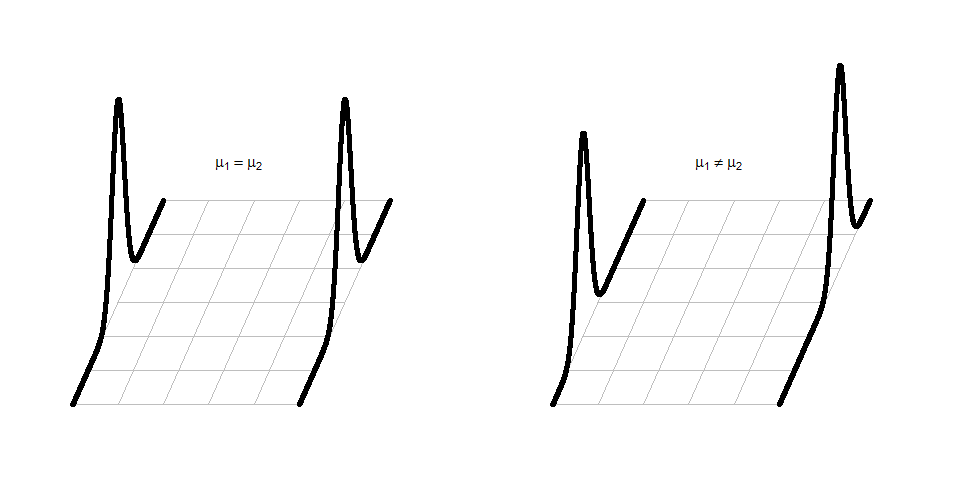
\includegraphics{chapter1_files/image015.png}
\caption{\label{fig:Figure2-7}Illustration of the assumed situations under the null
(left) and a single possibility that could occur if the alternative were
true (right) and the true means were different.}
\end{figure}

In statistical inference, null hypotheses (and their implied models) are
set up as ``straw men'' with every interest in rejecting them even
though we assume they are true to be able to assess the evidence against
them. Consider the original study design here, the pictures were
randomly assigned to the subjects. If the null hypothesis were true,
then we would have no difference in the population means of the groups.
And this would apply if we had done a different random assignment of the
pictures to the subjects. So let's try this: assume that the null
hypothesis is true and randomly re-assign the treatments (pictures) to
the observations that were obtained. In other words, keep the sentences
(\emph{Years}) the same and shuffle the group labels randomly. The
technical term for this is doing a \textbf{\emph{permutation}} (a random
shuffling of the treatments relative to the responses). If the null is
true and the means in the two groups are the same, then we should be
able to re-shuffle the groups to the observed sentences (\emph{Years})
and get results similar to those we actually observed. If the null is
false and the means are really different in the two groups, then what we
observed should differ from what we get under other random permutations.
The differences between the two groups should be more noticeable in the
observed data set than in (most) of the shuffled data sets. It helps to
see an example of a permutation of the labels to understand what this
means here.

In the \texttt{mosaic} package, the \texttt{shuffle} function allows us
to easily perform a permutation\footnote{We'll see the \texttt{shuffle}
  function in a more common usage below; while the code to generate
  \texttt{Perm1} is provided, it isn't something to worry about right
  now.}. Just one time, we can explore what a permutation of the
treatment labels could look like in the \texttt{PermutedAttr} variable
below. Note that the \texttt{Years} are held in the same place the group
labels are shuffled.

\begin{Shaded}
\begin{Highlighting}[]
\KeywordTok{set.seed}\NormalTok{(}\DecValTok{1234}\NormalTok{)}
\end{Highlighting}
\end{Shaded}

\begin{Shaded}
\begin{Highlighting}[]
\NormalTok{Perm1 <-}\StringTok{ }\KeywordTok{with}\NormalTok{(MockJury2,}\KeywordTok{data.frame}\NormalTok{(Years,Attr,}\DataTypeTok{PermutedAttr=}\KeywordTok{shuffle}\NormalTok{(Attr)))}
\NormalTok{Perm1}
\end{Highlighting}
\end{Shaded}

\begin{verbatim}
##    Years         Attr PermutedAttr
## 1      1 Unattractive Unattractive
## 2      4 Unattractive      Average
## 3      3 Unattractive      Average
## 4      2 Unattractive      Average
## 5      8 Unattractive      Average
## 6      8 Unattractive      Average
## 7      1 Unattractive Unattractive
## 8      1 Unattractive Unattractive
## 9      5 Unattractive      Average
## 10     7 Unattractive Unattractive
## 11     1 Unattractive      Average
## 12     5 Unattractive Unattractive
## 13     2 Unattractive Unattractive
## 14    12 Unattractive      Average
## 15    10 Unattractive      Average
## 16     1 Unattractive      Average
## 17     6 Unattractive Unattractive
## 18     2 Unattractive      Average
## 19     5 Unattractive Unattractive
## 20    12 Unattractive Unattractive
## 21     6 Unattractive      Average
## 22     3 Unattractive      Average
## 23     8 Unattractive      Average
## 24     4 Unattractive Unattractive
## 25    10 Unattractive Unattractive
## 26    10 Unattractive      Average
## 27    15 Unattractive Unattractive
## 28    15 Unattractive      Average
## 29     3 Unattractive      Average
## 30     3 Unattractive      Average
## 31     3 Unattractive Unattractive
## 32    11 Unattractive      Average
## 33    12 Unattractive      Average
## 34     2 Unattractive Unattractive
## 35     1 Unattractive Unattractive
## 36     1 Unattractive Unattractive
## 37    12 Unattractive      Average
## 38     5      Average Unattractive
## 39     5      Average Unattractive
## 40     4      Average Unattractive
## 41     3      Average Unattractive
## 42     6      Average      Average
## 43     4      Average      Average
## 44     9      Average      Average
## 45     8      Average Unattractive
## 46     3      Average      Average
## 47     2      Average Unattractive
## 48    10      Average      Average
## 49     1      Average Unattractive
## 50     1      Average Unattractive
## 51     3      Average Unattractive
## 52     1      Average      Average
## 53     3      Average      Average
## 54     5      Average      Average
## 55     8      Average Unattractive
## 56     3      Average      Average
## 57     1      Average      Average
## 58     1      Average Unattractive
## 59     1      Average      Average
## 60     2      Average      Average
## 61     2      Average Unattractive
## 62     1      Average      Average
## 63     1      Average Unattractive
## 64     2      Average Unattractive
## 65     3      Average Unattractive
## 66     4      Average Unattractive
## 67     5      Average      Average
## 68     3      Average Unattractive
## 69     3      Average      Average
## 70     3      Average      Average
## 71     2      Average Unattractive
## 72     7      Average Unattractive
## 73     6      Average Unattractive
## 74    12      Average Unattractive
## 75     8      Average      Average
\end{verbatim}

If you count up the number of subjects in each group by counting the
number of times each label (Average, Unattractive) occurs, it is the
same in both the \texttt{Attr} and \texttt{PermutedAttr} columns.
Permutations involve randomly re-ordering the values of a variable --
here the \texttt{Attr} group labels -- without changing the content of
the variable. This result can also be generated using what is called
\textbf{\emph{sampling without replacement}}: sequentially select \(n\)
labels from the original variable, removing each used label and making
sure that each original \texttt{Attr} label is selected once and only
once. The new, randomly selected order of selected labels provides the
permuted labels. Stepping through the process helps to understand how it
works: after the initial random sample of one label, there would
\(n - 1\) choices possible; on the \(n^{th}\) selection, there would
only be one label remaining to select. This makes sure that all original
labels are re-used but that the order is random. Sampling without
replacement is like picking names out of a hat, one-at-a-time, and not
putting the names back in after they are selected. It is an exhaustive
process for all the original observations. \textbf{\emph{Sampling with
replacement}} , in contrast, involves sampling from the specified list
with each observation having an equal chance of selection for each
sampled observation -- in other words, observations can be selected more
than once. This is like picking \(n\) names out of a hat that contains
\(n\) names, except that every time a name is selected, it goes back
into the hat -- we'll use this technique in Section \ref{section2-8} to
do what is called \textbf{\emph{bootstrapping}}. Both sampling
mechanisms can be used to generate inferences but each has particular
situations where they are most useful. For hypothesis testing, we will
use permutations (sampling without replacement).

The comparison of the beanplots for the real data set and permuted
version of the labels is what is really interesting (Figure
\ref{fig:Figure2-8}). The original difference in the sample means of the
two groups was 1.84 years (Unattractive minus Average). The sample means
are the \textbf{\emph{statistics}} that estimate the parameters for the
true means of the two groups. In the permuted data set, the difference
in the means is 1.15 years in the opposite direction (Average had a
higher mean than Unattractive in the permuted data).

\begin{Shaded}
\begin{Highlighting}[]
\KeywordTok{mean}\NormalTok{(Years }\OperatorTok{~}\StringTok{ }\NormalTok{PermutedAttr, }\DataTypeTok{data=}\NormalTok{Perm1)}
\end{Highlighting}
\end{Shaded}

\begin{verbatim}
##      Average Unattractive 
##     5.447368     4.297297
\end{verbatim}

\begin{Shaded}
\begin{Highlighting}[]
\KeywordTok{diffmean}\NormalTok{(Years }\OperatorTok{~}\StringTok{ }\NormalTok{PermutedAttr, }\DataTypeTok{data=}\NormalTok{Perm1)}
\end{Highlighting}
\end{Shaded}

\begin{verbatim}
##  diffmean 
## -1.150071
\end{verbatim}




\begin{figure}
\centering
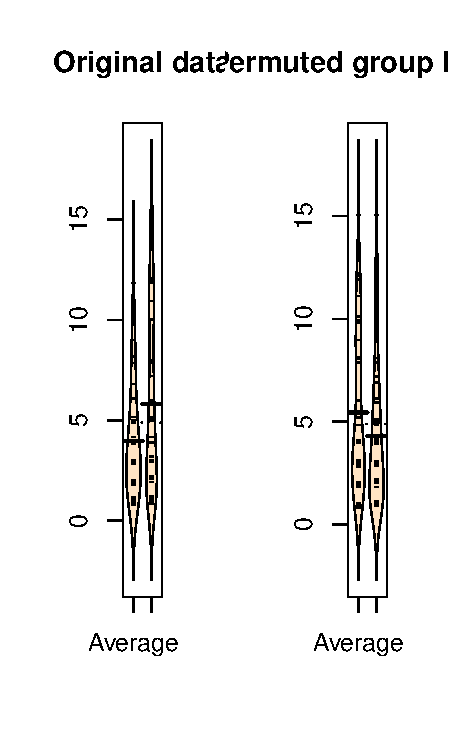
\includegraphics{02-reintroductionToStatistics_files/figure-latex/Figure2-8-1.pdf}
\caption{\label{fig:Figure2-8}Boxplots of Years responses versus actual treatment groups
and permuted groups.}
\end{figure}

These results suggest that the observed difference was larger than what
we got when we did a single permutation although it was only a little
bit larger than a difference we could observe in permutations if we
ignore the difference in directions. Conceptually, permuting
observations between group labels is consistent with the null hypothesis
-- this is a technique to generate results that we might have gotten if
the null hypothesis were true since the responses are the same in the
two groups if the null is true. We just need to repeat the permutation
process many times and track how unusual our observed result is relative
to this distribution of potential responses if the null were true. If
the observed differences are unusual relative to the results under
permutations, then there is evidence against the null hypothesis, the
null hypothesis should be rejected ( Reject \(H_0\)), and a conclusion
should be made, in the direction of the alternative hypothesis, that
there is evidence that the true means differ. If the observed
differences are similar to (or at least not unusual relative to) what we
get under random shuffling under the null model, we would have a tough
time concluding that there is any real difference between the groups
based on our observed data set.

\section{Permutation testing for the 2 sample mean
situation}\label{section2-4}

In any testing situation, you must define some function of the
observations that gives us a single number that addresses our question
of interest. This quantity is called a \textbf{\emph{test statistic}}.
These often take on complicated forms and have names like \(t\) or \(z\)
statistics that relate to their parametric (named) distributions so we
know where to look up \textbf{\emph{p-values}}\footnote{P-values are the
  probability of obtaining a result as extreme as or more extreme than
  we observed given that the null hypothesis is true.}. In randomization
settings, they can have simpler forms because we use the data set to
find the distribution of the statistic and don't need to rely on a named
distribution. We will label our test statistic \textbf{\emph{T}} (for
\textbf{T} statistic) unless the test statistic has a commonly used
name. Since we are interested in comparing the means of the two groups,
we can define

\[T=\bar{x}_{Unattractive}-\bar{x}_{Average},\]

which coincidentally is what the\texttt{diffmean} function provided us
previously. We label our \textbf{\emph{observed test statistic}} (the
one from the original data set) as

\[T_{obs}=\bar{x}_{Unattractive}-\bar{x}_{Average},\]

which happened to be 1.84 years here. We will compare this result to the
results for the test statistic that we obtain from permuting the group
labels. To denote permuted results, we will add a * to the labels:

\[T^*=\bar{x}_{Unattractive}-\bar{x}_{Average^*}.\]

We then compare the
\(T_{obs}=\bar{x}_{Unattractive}-\bar{x}_{Average} = 1.84\) to the
distribution of results that are possible for the permuted results
(\(T^*\)) which corresponds to assuming the null hypothesis is true.

We need to consider lots of permutations to do a permutation test. In
contrast to your introductory statistics course where, if you did this,
it was just a click away, we are going to learn what was going on under
the hood. Specifically, we need a \textbf{\emph{for loop}} in R to be
able to repeatedly generate the permuted data sets and record \(T^*\)
for each one. Loops are a basic programming task that make randomization
methods possible as well as potentially simplifying any repetitive
computing task. To write a ``for loop'', we need to choose how many
times we want to do the loop (call that \texttt{B}) and decide on a
counter to keep track of where we are at in the loops (call that
\texttt{b}, which goes from 1 up to \texttt{B}). The simplest loop just
involves printing out the index, \texttt{print(b)} at each step. This is
our first use of curly braces, \{ and\}, that are used to group the code
we want to repeatedly run as we proceed through the loop. By typing the
following code in the script window and then highlighting it all and
hitting the run button, R will go through the loop 5 times, printing out
the counter:

\begin{verbatim}
B <- 5
for (b in (1:B)){
  print(b)
}
\end{verbatim}

Note that when you highlight and run the code, it will look about the
same with ``+'' printed after the first line to indicate that all the
code is connected when it appears in the console, looking like this:

\begin{Shaded}
\begin{Highlighting}[]
\OperatorTok{>}\StringTok{ }\ControlFlowTok{for}\NormalTok{(b }\ControlFlowTok{in}\NormalTok{ (}\DecValTok{1}\OperatorTok{:}\NormalTok{B))\{}
\OperatorTok{+}\StringTok{   }\KeywordTok{print}\NormalTok{(b)}
\OperatorTok{+}\NormalTok{\}}
\end{Highlighting}
\end{Shaded}

When you run these three lines of code, the console will show you the
following output:

\begin{Shaded}
\begin{Highlighting}[]
\NormalTok{[}\DecValTok{1}\NormalTok{] }\DecValTok{1}
\NormalTok{[}\DecValTok{1}\NormalTok{] }\DecValTok{2}
\NormalTok{[}\DecValTok{1}\NormalTok{] }\DecValTok{3}
\NormalTok{[}\DecValTok{1}\NormalTok{] }\DecValTok{4}
\NormalTok{[}\DecValTok{1}\NormalTok{] }\DecValTok{5}
\end{Highlighting}
\end{Shaded}

Instead of printing the counter, we want to use the loop to repeatedly
compute our test statistic across B random permutations of the
observations. The \texttt{shuffle} function performs permutations of the
group labels relative to responses and the \texttt{diffmean} difference
in the two group means in the permuted data set. For a single
permutation, the combination of shuffling \texttt{Attr} and finding the
difference in the means, storing it in a variable called \texttt{Ts} is:

\begin{Shaded}
\begin{Highlighting}[]
\NormalTok{Ts <-}\StringTok{ }\KeywordTok{diffmean}\NormalTok{(Years }\OperatorTok{~}\StringTok{ }\KeywordTok{shuffle}\NormalTok{(Attr), }\DataTypeTok{data=}\NormalTok{MockJury2)}
\NormalTok{Ts}
\end{Highlighting}
\end{Shaded}

\begin{verbatim}
##  diffmean 
## -0.616643
\end{verbatim}

And putting this inside the \texttt{print} function allows us to find
the test statistic under 5 different permutations easily:

\begin{Shaded}
\begin{Highlighting}[]
\NormalTok{B <-}\StringTok{ }\DecValTok{5}
\ControlFlowTok{for}\NormalTok{ (b }\ControlFlowTok{in}\NormalTok{ (}\DecValTok{1}\OperatorTok{:}\NormalTok{B))\{}
\NormalTok{  Ts <-}\StringTok{ }\KeywordTok{diffmean}\NormalTok{(Years }\OperatorTok{~}\StringTok{ }\KeywordTok{shuffle}\NormalTok{(Attr), }\DataTypeTok{data=}\NormalTok{MockJury2)}
  \KeywordTok{print}\NormalTok{(Ts)}
\NormalTok{\}}
\end{Highlighting}
\end{Shaded}

\begin{verbatim}
##   diffmean 
## -0.8300142 
##   diffmean 
## -0.1365576 
##    diffmean 
## -0.08321479 
##  diffmean 
## 0.5035562 
## diffmean 
## 1.677098
\end{verbatim}

Finally, we would like to store the values of the test statistic instead
of just printing them out on each pass through the loop. To do this, we
need to create a variable to store the results, let's call it
\texttt{Tstar}. We know that we need to store \texttt{B} results so will
create a vector of length B, which contains B elements, full of missing
values (NA) using the \texttt{matrix} function:

\begin{Shaded}
\begin{Highlighting}[]
\NormalTok{Tstar <-}\StringTok{ }\KeywordTok{matrix}\NormalTok{(}\OtherTok{NA}\NormalTok{, }\DataTypeTok{nrow=}\NormalTok{B)}
\NormalTok{Tstar}
\end{Highlighting}
\end{Shaded}

\begin{verbatim}
##      [,1]
## [1,]   NA
## [2,]   NA
## [3,]   NA
## [4,]   NA
## [5,]   NA
\end{verbatim}

Now we can run our loop B times and store the results in \texttt{Tstar}.

\begin{Shaded}
\begin{Highlighting}[]
\ControlFlowTok{for}\NormalTok{ (b }\ControlFlowTok{in}\NormalTok{ (}\DecValTok{1}\OperatorTok{:}\NormalTok{B))\{}
\NormalTok{  Tstar[b] <-}\StringTok{ }\KeywordTok{diffmean}\NormalTok{(Years }\OperatorTok{~}\StringTok{ }\KeywordTok{shuffle}\NormalTok{(Attr), }\DataTypeTok{data=}\NormalTok{MockJury2)}
\NormalTok{\}}
\NormalTok{Tstar}
\end{Highlighting}
\end{Shaded}

\begin{verbatim}
##             [,1]
## [1,] -0.08321479
## [2,]  0.23684211
## [3,] -0.24324324
## [4,] -0.61664296
## [5,]  0.66358464
\end{verbatim}

Five permutations are still not enough to assess whether our \(T_{obs}\)
of 1.84 is unusual and we need to do many permutations to get an
accurate assessment of the possibilities under the null hypothesis. It
is common practice to consider something like 1,000 permutations. The
\texttt{Tstar} vector when we set \emph{B} the permutation distribution
for the selected test statistic under\footnote{We often say ``under'' in
  statistics and we mean ``given that the following is true''.} the null
hypothesis -- what is called the \textbf{\emph{null distribution}} of
the statistic. The null distribution is the distribution of possible
values of a statistic under the null hypothesis. We want to visualize
this distribution and use it to assess how unusual our \(T_{obs}\)
result of 1.84 years was relative to all the possibilities under
permutations (under the null hypothesis). So we repeat the loop, now
with \(B=1000\) and generate a histogram, density curve and summary
statistics of the results:




\begin{figure}
\centering
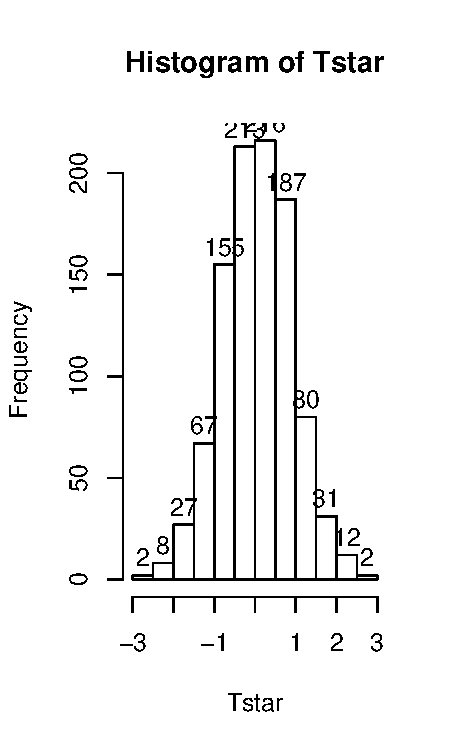
\includegraphics{02-reintroductionToStatistics_files/figure-latex/Figure2-9-1.pdf}
\caption{\label{fig:Figure2-9}Histogram (left, with counts in bars) and density curve
(right) of values of test statistic for 1,000 permutations.}
\end{figure}

\begin{Shaded}
\begin{Highlighting}[]
\KeywordTok{par}\NormalTok{(}\DataTypeTok{mfrow=}\KeywordTok{c}\NormalTok{(}\DecValTok{1}\NormalTok{,}\DecValTok{2}\NormalTok{))}
\NormalTok{B <-}\StringTok{ }\DecValTok{1000}
\NormalTok{Tstar <-}\StringTok{ }\KeywordTok{matrix}\NormalTok{(}\OtherTok{NA}\NormalTok{, }\DataTypeTok{nrow=}\NormalTok{B)}
\ControlFlowTok{for}\NormalTok{ (b }\ControlFlowTok{in}\NormalTok{ (}\DecValTok{1}\OperatorTok{:}\NormalTok{B))\{}
\NormalTok{  Tstar[b] <-}\StringTok{ }\KeywordTok{diffmean}\NormalTok{(Years }\OperatorTok{~}\StringTok{ }\KeywordTok{shuffle}\NormalTok{(Attr), }\DataTypeTok{data=}\NormalTok{MockJury2)}
\NormalTok{\}}
\KeywordTok{hist}\NormalTok{(Tstar, }\DataTypeTok{label=}\NormalTok{T)}
\KeywordTok{plot}\NormalTok{(}\KeywordTok{density}\NormalTok{(Tstar), }\DataTypeTok{main=}\StringTok{"Density curve of Tstar"}\NormalTok{)}
\end{Highlighting}
\end{Shaded}

\begin{Shaded}
\begin{Highlighting}[]
\KeywordTok{favstats}\NormalTok{(Tstar)}
\end{Highlighting}
\end{Shaded}

\begin{verbatim}
##        min         Q1     median        Q3      max       mean        sd
##  -2.910384 -0.5099573 0.07681366 0.6102418 2.530583 0.04694168 0.8497364
##     n missing
##  1000       0
\end{verbatim}

Figure \ref{fig:Figure2-9} contains visualizations of \(T^*\) and the
\texttt{favstats} summary provides the related numerical summaries. Our
observed \(T_{obs}\) of 1.84 seems fairly unusual relative to these
results with only 20 \(T^*\) values over 2 based on the histogram. We
need to make more specific comparisons of the permuted results versus
our observed result to be able to clearly decide whether our observed
result is really unusual.

To make the comparisons more concrete, first we can enhance the previous
graphs by adding the value of the test statistic from the real data set,
as shown in Figure \ref{fig:Figure2-10}, using the \texttt{abline}
function.





\begin{figure}
\centering
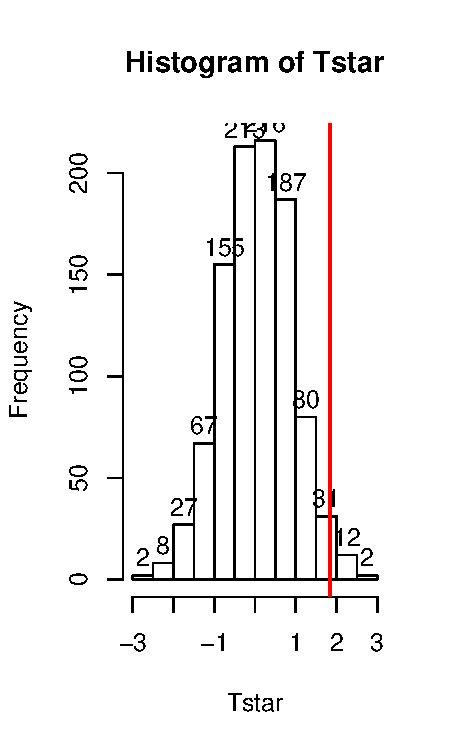
\includegraphics{02-reintroductionToStatistics_files/figure-latex/Figure2-10-1.pdf}
\caption{\label{fig:Figure2-10}Histogram (left) and density curve (right) of values of
test statistic for 1,000 permutations with bold vertical line for value
of observed test statistic.}
\end{figure}

\begin{Shaded}
\begin{Highlighting}[]
\KeywordTok{par}\NormalTok{(}\DataTypeTok{mfrow=}\KeywordTok{c}\NormalTok{(}\DecValTok{1}\NormalTok{,}\DecValTok{2}\NormalTok{))}
\NormalTok{Tobs <-}\StringTok{ }\FloatTok{1.837}
\KeywordTok{hist}\NormalTok{(Tstar, }\DataTypeTok{labels=}\NormalTok{T)}
\KeywordTok{abline}\NormalTok{(}\DataTypeTok{v=}\NormalTok{Tobs, }\DataTypeTok{lwd=}\DecValTok{2}\NormalTok{, }\DataTypeTok{col=}\StringTok{"red"}\NormalTok{)}
\KeywordTok{plot}\NormalTok{(}\KeywordTok{density}\NormalTok{(Tstar),}\DataTypeTok{main=}\StringTok{"Density curve of Tstar"}\NormalTok{)}
\KeywordTok{abline}\NormalTok{(}\DataTypeTok{v=}\NormalTok{Tobs, }\DataTypeTok{lwd=}\DecValTok{2}\NormalTok{, }\DataTypeTok{col=}\StringTok{"red"}\NormalTok{)}
\end{Highlighting}
\end{Shaded}

Second, we can calculate the exact number of permuted results that were
larger than what we observed. To calculate the proportion of the 1,000
values that were larger than what we observed, we will use the
\texttt{pdata} function. To use this function, we need to provide the
distribution of values to compare to the cut-off (\texttt{Tstar}), the
cut-off point (\texttt{Tobs}), and whether we want calculate the
proportion that are below (left of) or above (right of) the cut-off
(\texttt{lower.tail=F} option provides the proportion of values above
the cutoff of interest).

\begin{Shaded}
\begin{Highlighting}[]
\KeywordTok{pdata}\NormalTok{(Tstar, Tobs, }\DataTypeTok{lower.tail=}\NormalTok{F)}
\end{Highlighting}
\end{Shaded}

\begin{verbatim}
## [1] 0.02
\end{verbatim}

The proportion of 0.02 tells us that 20 of the 1,000 permuted results
(2\%) were larger than what we observed. This type of work is how we can
generate \textbf{\emph{p-values}} using permutation distributions.
P-values, as you should remember, are the probability of getting a
result as extreme as or more extreme than what we observed, given that
the null is true. Finding only 20 permutations of 1,000 that were larger
than our observed result suggests that it is hard to find a result like
what we observed if there really were no difference, although it is not
impossible.

When testing hypotheses for two groups, there are two types of
alternative hypotheses, one-sided or two-sided. \textbf{\emph{One-sided
tests}} involve only considering differences in one-direction (like
\(\mu_1 > \mu_2\)) and are performed when researchers can decide
\textbf{\emph{a priori}}\footnote{This is a fancy way of saying ``in
  advance'', here in advance of seeing the observations.} which group
should have a larger mean if there is going to be any sort of
difference. In this situation, we did not know enough about the
potential impacts of the pictures to know which group should be larger
than the other so should do a two-sided test. It is important to
remember that you can't look at the responses to decide on the
hypotheses. It is often safer and more
\textbf{\emph{conservative}}\footnote{Statistically, a conservative
  method is one that provides less chance of rejecting the null
  hypothesis in comparison to some other method or less than some
  pre-defined standard.} to start with a \textbf{\emph{two-sided
alternative}} (\(\mathbf{H_A: \mu_1 \ne \mu_2}\)). To do a 2-sided test,
find the area larger than what we observed as above. We also need to add
the area in the other tail (here the left tail) similar to what we
observed in the right tail. Some people suggest doubling the area in one
tail but we will collect information on the number that were more
extreme than the same value in the other tail. In other words, we count
the proportion over 1.84 and below -1.84. So we need to also find how
many of the permuted results were smaller than -1.84years to add to our
previous proportion. Using \texttt{pdata} \texttt{-Tobs} as the cut-off
and \texttt{lower.tail=T} provides this result:

\begin{Shaded}
\begin{Highlighting}[]
\KeywordTok{pdata}\NormalTok{(Tstar, }\OperatorTok{-}\NormalTok{Tobs, }\DataTypeTok{lower.tail=}\NormalTok{T)}
\end{Highlighting}
\end{Shaded}

\begin{verbatim}
## [1] 0.014
\end{verbatim}

So the p-value to test our null hypothesis of no difference in the true
means between the groups is 0.02 + 0.014, providing a p-value of 0.034.
Figure \ref{fig:Figure2-11} shows both cut-offs on the histogram and
density curve.





\begin{figure}
\centering
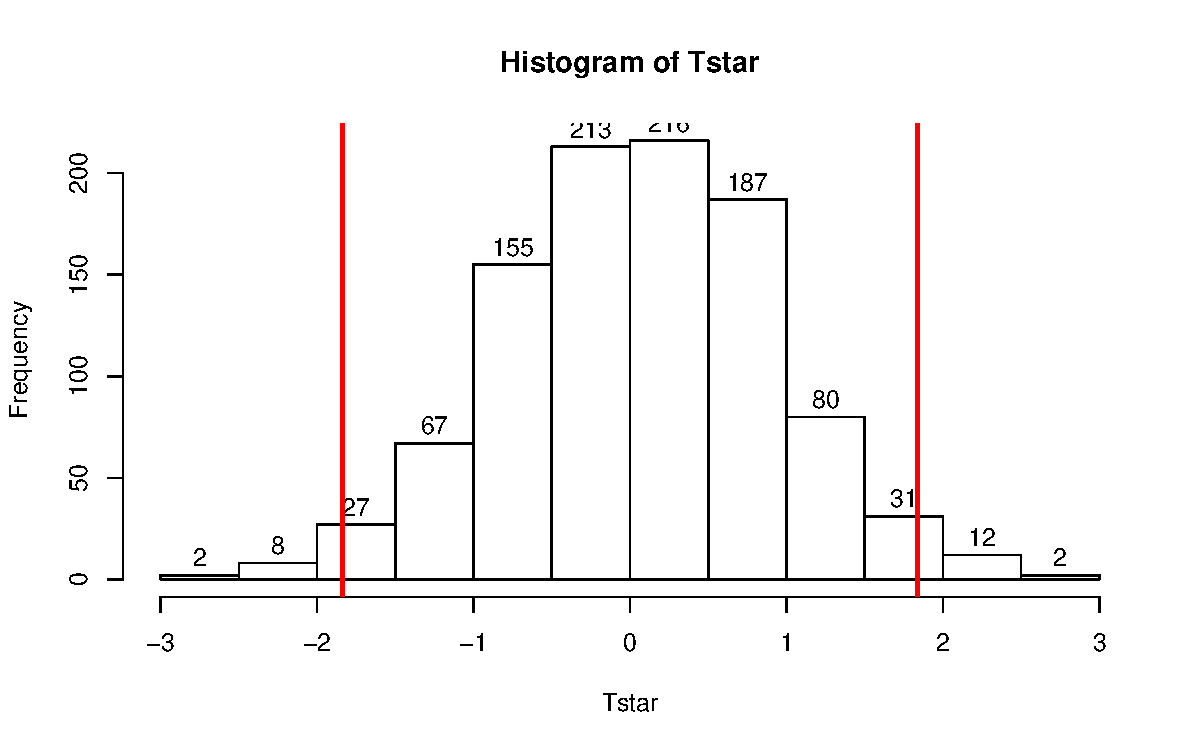
\includegraphics{02-reintroductionToStatistics_files/figure-latex/Figure2-11-1.pdf}
\caption{\label{fig:Figure2-11}Histogram and density curve of values of test statistic
for 1,000 permutations with bold lines for value of observed test
statistic and its opposite value required for performing two-sided test.}
\end{figure}

\begin{Shaded}
\begin{Highlighting}[]
\KeywordTok{par}\NormalTok{(}\DataTypeTok{mfrow=}\KeywordTok{c}\NormalTok{(}\DecValTok{1}\NormalTok{,}\DecValTok{2}\NormalTok{))}
\KeywordTok{hist}\NormalTok{(Tstar, }\DataTypeTok{labels=}\NormalTok{T)}
\KeywordTok{abline}\NormalTok{(}\DataTypeTok{v=}\KeywordTok{c}\NormalTok{(}\OperatorTok{-}\DecValTok{1}\NormalTok{,}\DecValTok{1}\NormalTok{)}\OperatorTok{*}\NormalTok{Tobs, }\DataTypeTok{lwd=}\DecValTok{2}\NormalTok{, }\DataTypeTok{col=}\StringTok{"red"}\NormalTok{)}
\KeywordTok{plot}\NormalTok{(}\KeywordTok{density}\NormalTok{(Tstar),}\DataTypeTok{main=}\StringTok{"Density curve of Tstar"}\NormalTok{)}
\KeywordTok{abline}\NormalTok{(}\DataTypeTok{v=}\KeywordTok{c}\NormalTok{(}\OperatorTok{-}\DecValTok{1}\NormalTok{,}\DecValTok{1}\NormalTok{)}\OperatorTok{*}\NormalTok{Tobs, }\DataTypeTok{lwd=}\DecValTok{2}\NormalTok{, }\DataTypeTok{col=}\StringTok{"red"}\NormalTok{)}
\end{Highlighting}
\end{Shaded}

In general, the \textbf{\emph{one-sided test p-value}} is the proportion
of the permuted results that are more extreme than observed in the
direction of the \emph{alternative} hypothesis (lower or upper tail,
remembering that this also depends on the direction of the difference
taken). For the 2-sided test, the p-value is the proportion of the
permuted results that are \emph{less than the negative version of the
observed statistic and greater than the positive version of the observed
statistic}. Using absolute values (\textbar{} \textbar{}), we can
simplify this: the \textbf{\emph{two-sided p-value}} is the
\emph{proportion of the \textbar{}permuted statistics\textbar{} that are
larger than \textbar{}observed statistic\textbar{}}. This will always
work and finds areas in both tails regardless of whether the observed
statistic is positive or negative. In R, the \texttt{abs} function
provides the \textbf{\emph{absolute value}} and we can again use
\texttt{pdata} to find our p-value in one line of code:

\begin{Shaded}
\begin{Highlighting}[]
\KeywordTok{pdata}\NormalTok{(}\KeywordTok{abs}\NormalTok{(Tstar), }\KeywordTok{abs}\NormalTok{(Tobs), }\DataTypeTok{lower.tail=}\NormalTok{F)}
\end{Highlighting}
\end{Shaded}

\begin{verbatim}
## [1] 0.034
\end{verbatim}

We will discuss the choice of \textbf{\emph{significance level}} below,
but for the moment, assume that \(\alpha\) is chosen to be our standard
value of 0.05. Since the p-value is smaller than \(\alpha\), this
suggests that we can \textbf{\emph{reject the null hypothesis}} and
conclude that there is evidence of some difference in the true mean
sentences given between the two types of pictures.

Before we move on, let's note some interesting features of the
permutation distribution of the difference in the sample means shown in
Figure \ref{fig:Figure2-11}.

\begin{enumerate}
\def\labelenumi{\arabic{enumi}.}
\item
  It is basically centered at 0. Since we are performing permutations
  assuming the null model is true, we are assuming that
  \(\mu_1 = \mu_2\) which implies that \(\mu_1 - \mu_2 = 0\). This also
  suggests that 0 should be the center of the permutation distribution
  and it was.
\item
  It is approximately normally distributed. This is due to the
  \textbf{\emph{Central Limit Theorem}}\footnote{We'll leave the
    discussion of the CLT to your previous stat coursework or an
    internet search. Remember that it has something to do with
    distributions looking more normal as the sample size increases.},
  where the \textbf{\emph{sampling distribution}} (distribution of all
  possible results for samples of this size) of the difference in sample
  means (\(\bar{x}_1 - \bar{x}_2\)) becomes more and normally
  distributed as the sample sizes increase. With 38 and 37 observations
  in the groups, we are likely to have a relatively normal looking
  distribution of the difference in the sample means. This result will
  allow us to use a parametric method to approximate this sampling
  distribution under the null model if some assumptions are met, as
  we'll discuss below.
\item
  Our observed difference in the sample means (1.84 years) is a fairly
  unusual result relative to the rest of these results but there are
  some permuted data sets that produce more extreme differences in the
  sample means. When the observed differences are really large, we may
  not see any permuted results that are as extreme as what we observed.
  When \texttt{pdata} gives you 0, the p-value should be reported to be
  smaller than 0.0001 (\textbf{not 0!}) since it happened in less than 1
  in 1000 tries but does occur once -- in the actual data set.
\item
  Since our null model is not specific about the direction of the
  difference, considering a result like ours but in the other direction
  (-1.84 years) needs to be included. The observed result seems to put
  about the same area in both tails of the distribution but it is not
  exactly the same. The small difference in the tails is a useful aspect
  of this approach compared to the parametric method discussed below as
  it accounts for slight asymmetry in the sampling distribution.
\end{enumerate}

Earlier, we decided that the p-value was small enough to reject the null
hypothesis since it was smaller than our chosen level of significance.
In this course, you will often be allowed to use your own judgment about
an appropriate significance level in a particular situation (in other
words, if we forget to tell you an \(\alpha\) -level, you can still make
a decision using a reasonably selected significance level). Remembering
that the p-value is the probability you would observe a result like you
did (or more extreme), assuming the null hypothesis is true, this tells
you that the smaller the p-value is, the more evidence you have against
the null. The next section provides a more formal review of the
hypothesis testing infrastructure, terminology, and some of things that
can happen when testing hypotheses.

\section{Hypothesis testing (general)}\label{section2-5}

In hypothesis testing, it is formulated to answer a specific question
about a population or true parameter(s) using a statistic based on a
data set. In your previous statistics course, you (hopefully) considered
one-sample hypotheses about population means and proportions and the two
sample mean situation we are focused on here. Our hypotheses relate to
trying to answer the question about whether the population mean
sentences between the two groups are different, with an initial
assumption of no difference.

Hypothesis testing is much like a criminal trial where you are in the
role of a jury member or judge, if no jury is present. Initially, the
defendant is assumed innocent. In our situation, the true means are
assumed to be equal between the groups. Then evidence is presented and,
as a juror, you analyze it. In statistical hypothesis testing, data are
collected and analyzed. Then you have to decide if we had ``enough''
evidence to reject the initial assumption (``innocence'' that is
initially assumed). To make this decision, you want to have previously
decided on the standard of evidence required to reject the initial
assumption. In criminal cases, ``beyond a reasonable doubt'' is used.
Wikipedia's definition
(\url{https://en.wikipedia.org/wiki/Reasonable_doubt}) suggests that
this standard is that ``there can still be a doubt, but only to the
extent that it would not affect a reasonable person's belief regarding
whether or not the defendant is guilty''. In civil trials, a lower
standard called a ``preponderance of evidence'' is used. Based on that
defined and pre-decided (\emph{a priori}) measure, you decide that the
defendant is guilty or not guilty. In statistics, we compare our p-value
to a significance level, \(\alpha\), which is most of the time selected
to be 5\%. If our p-value is less than \(\alpha\), we reject the null
hypothesis. The choice of the significance level is like the variation
in standards of evidence between criminal and civil trials -- and in all
situations everyone should know the standards required for rejecting the
initial assumption before any information is ``analyzed''. Once someone
is found guilty, then there is the matter of sentencing which is related
to the impacts (``size'') of the crime. In statistics, this is similar
to the estimated size of differences and the related judgments about
whether the differences are practically important or not. If the crime
is proven beyond a reasonable doubt but it is a minor crime, then the
sentence will be small. With the same level of evidence and a more
serious crime, the sentence will be more dramatic.

There are some important aspects of the testing process to note that
inform how we interpret statistical hypothesis test results. When
someone is found ``not guilty'', it does not mean ``innocent'', it just
means that there was not enough evidence to find the person guilty
``beyond a reasonable doubt''. Not finding enough evidence to reject the
null hypothesis does not imply that the true means are equal, just that
there was not enough evidence to conclude that they were different.
There are many potential reasons why we might fail to reject the null,
but the most common one is that our sample size was too small (which is
related to having too little evidence).

Throughout this material, we will continue to re-iterate the
distinctions between parameters and statistics and want you to be clear
about the distinctions between estimates based on the sample and
inferences for the population or true values of the parameters of
interest. Remember that statistics are summaries of the sample
information and parameters are characteristics of populations (which we
rarely know). In the two-sample mean situation, the sample means are
always at least a little different -- that is not an interesting
conclusion. What is interesting is whether we have enough evidence to
prove that the population or true means differ ``beyond a reasonable
doubt''.

The scope of any inferences is constrained based on whether there is a
\textbf{\emph{random sample}} (RS) and/or \textbf{\emph{random
assignment}} (RA). Table \ref{tab:Table2-2} contains the four possible
combinations of these two characteristics of a given study. Random
assignment allows for causal inferences for differences that are
observed -- the difference in treatment levels causes differences in the
mean responses. Random sampling (or at least some sort of representative
sample) allows inferences to be made to the population of interest. If
we do not have RA, then causal inferences cannot be made. If we do not
have a representative sample, then our inferences are limited to the
sampled subjects.

\footnotesize



\begin{longtable}[]{@{}lll@{}}
\caption{\label{tab:Table2-2} Scope of inference summary.}\tabularnewline
\toprule
\begin{minipage}[b]{0.27\columnwidth}\raggedright\strut
\textbf{Random\\
Sampling/Random\\
Assignment}\strut
\end{minipage} & \begin{minipage}[b]{0.31\columnwidth}\raggedright\strut
\textbf{Random Assignment (RA)\\
-- Yes (controlled experiment)}\strut
\end{minipage} & \begin{minipage}[b]{0.33\columnwidth}\raggedright\strut
\textbf{Random Assignment (RA)\\
-- No (observational study)}\strut
\end{minipage}\tabularnewline
\midrule
\endfirsthead
\toprule
\begin{minipage}[b]{0.27\columnwidth}\raggedright\strut
\textbf{Random\\
Sampling/Random\\
Assignment}\strut
\end{minipage} & \begin{minipage}[b]{0.31\columnwidth}\raggedright\strut
\textbf{Random Assignment (RA)\\
-- Yes (controlled experiment)}\strut
\end{minipage} & \begin{minipage}[b]{0.33\columnwidth}\raggedright\strut
\textbf{Random Assignment (RA)\\
-- No (observational study)}\strut
\end{minipage}\tabularnewline
\midrule
\endhead
\begin{minipage}[t]{0.27\columnwidth}\raggedright\strut
\textbf{Random Sampling (RS)\\
-- Yes (or some method\\
that results in a\\
representative sample of\\
population of\\
interest)}\strut
\end{minipage} & \begin{minipage}[t]{0.31\columnwidth}\raggedright\strut
Because we have RS, we can\\
generalize inferences to the\\
population the RS was taken\\
from. Because we have\\
RA we can assume the groups\\
were equivalent on all aspects\\
except for the treatment\\
and can establish causal inference.\\
\strut
\end{minipage} & \begin{minipage}[t]{0.33\columnwidth}\raggedright\strut
Can generalize inference to\\
population the RS was taken\\
from but cannot establish\\
causal inference (no RA\\
-- cannot isolate treatment\\
variable as only difference\\
among groups, could be\\
confounding variables).\strut
\end{minipage}\tabularnewline
\begin{minipage}[t]{0.27\columnwidth}\raggedright\strut
\textbf{Random Sampling (RS)\\
-- No (usually a\\
convenience sample)}\strut
\end{minipage} & \begin{minipage}[t]{0.31\columnwidth}\raggedright\strut
Cannot generalize inference to\\
the population of interest\\
because the sample was\\
not random and could be\\
biased -- may not be\\
``representative'' of the\\
population of interest.\\
Can establish causal\\
inference due to RA \(\rightarrow\)\\
the inference from this type of\\
study applies only to the sample.\strut
\end{minipage} & \begin{minipage}[t]{0.33\columnwidth}\raggedright\strut
Cannot generalize inference to\\
the population of interest\\
because the sample was\\
not random and could be\\
biased -- may not be\\
``representative'' of the\\
population of interest.\\
Cannot establish causal\\
inference due to lack of RA of\\
the treatment.\strut
\end{minipage}\tabularnewline
\bottomrule
\end{longtable}

\normalsize

A simple example helps to clarify how the scope of inference can change.
Suppose we are interested in studying the GPA of students. If we had
taken a random sample from, say, the STAT 217 students in a given
semester, our scope of inference would be the population of 217 students
in that semester. If we had taken a random sample from the entire MSU
population, then the inferences would be to the entire MSU population in
that semester. These are similar types of problems but the two
populations are very different and the group you are trying to make
conclusions about should be noted carefully in your results -- it does
matter! If we did not have a representative sample, say the students
could choose to provide this information or not, then we can only make
inferences to volunteers. These volunteers might differ in systematic
ways from the entire population of STAT 217 students so we cannot safely
extend our inferences beyond the group that volunteered.

To consider the impacts of RA versus observational studies, we need to
be comparing groups. Suppose that we are interested in differences in
the mean GPAs for different sections of STAT 217 and that we take a
random sample of students from each section and compare the results and
find evidence of some difference. In this scenario, we can conclude that
there is some difference in the population of STAT 217 students but we
can't say that being in different sections caused the differences in the
mean GPAs. Now suppose that we randomly assigned every 217 student to
get extra training in one of three different study techniques and found
evidence of differences among the training methods. We could conclude
that the training methods caused the differences in these students.
These conclusions would only apply to STAT 217 students and could not be
generalized to a larger population of students. If we took a random
sample of STAT 217 students (say only 10 from each section) and then
randomly assigned them to one of three training programs and found
evidence of differences, then we can say that the training programs
caused the differences. We can also say that we have evidence that those
differences pertain to the population of STAT 217 students. This seems
similar to the scenario where all 217 students participated in the
training programs except that by using random sampling, only a fraction
of the population needs to actually be studied to make inferences to the
entire population of interest -- saving time and money.

A quick summary of the terminology of hypothesis testing is useful at
this point. The \textbf{\emph{null hypothesis}} (\(H_0\)) states that
there is no difference or no relationship in the population. This is the
statement of no effect or no difference and the claim that we are trying
to find evidence against. In this chapter, \(H_0\): \(\mu_1=\mu_2\).
When doing two-group problems, you always need to specify which group is
1 and which one is 2 because the order does matter. The
\textbf{\emph{alternative hypothesis}} (\(H_1\) or \(H_A\)) states a
specific difference between parameters. This is the research hypothesis
and the claim about the population that we hope to demonstrate is more
reasonable to conclude than the null hypothesis. In the two-group
situation, we can have \textbf{\emph{one-sided alternatives}}
\(H_A\):\(\mu_1 > \mu_2\) (greater than) or \(H_A\):\(\mu_1 < \mu_2\)
(less than) or, the more common, \textbf{\emph{two-sided alternative}}
\(H_A\):\(\mu_1 \ne \mu_2\) (not equal to). We usually default to using
two-sided tests because we often do not know enough to know the
direction of a difference in advance, especially in more complicated
situations. The \textbf{\emph{sampling distribution under the null}} is
the distribution of all possible values of a statistic under \(H_0\) is
true. It is used to calculate the \textbf{\emph{p-value}} , the
probability of obtaining a result as extreme or more extreme than what
we observed given that the null hypothesis is true. We will find
sampling distributions using \textbf{\emph{nonparametric}} approaches
(like the permutation approach used above) and
\textbf{\emph{parametric}} methods (using ``named'' distributions like
the \(t\), F, and \(\chi^2\)).

Small p-values are evidence against the null hypothesis because the
observed result is unlikely due to chance if \(H_0\) is true. Large
p-values provide no evidence against \(H_0\) but do not allow us to
conclude that there is no difference. The \textbf{\emph{level of
significance}} is an \emph{a priori} definition of how small the p-value
needs to be to provide ``enough'' (sufficient) evidence against \(H_0\).
This is most useful to prevent sliding the standards after the results
are found. We compare the p-value to the level of significance to decide
if the p-value is small enough to constitute sufficient evidence to
reject the null hypothesis. We use \(\alpha\) to denote the level of
significance and most typically use 0.05 which we refer to as the 5\%
significance level. We compare the p-value to this level and make a
decision. The two options for \emph{decisions} are to either
\emph{reject the null hypothesis} if the p-value \(\le \alpha\) or
\emph{fail to reject the null hypothesis} if the p-value \(> \alpha\).
When interpreting hypothesis testing results, remember that the p-value
is a measure of how unlikely the observed outcome was, assuming that the
null hypothesis is true. It is \textbf{NOT} the probability of the data
or the probability of either hypothesis being true. The p-value, simply,
is a measure of evidence against the null hypothesis.

The specific definition of \(\alpha\) is that it is the probability of
rejecting \(H_0\) when \(H_0\) is true, the probability of what is
called a \textbf{\emph{Type I error}}. Type I errors are also called
\textbf{\emph{false rejections}}. In the two-group mean situation, a
Type I error would be concluding that there is a difference in the true
means between the groups when none really exists in the population. In
the courtroom setting, this is like falsely finding someone guilty. We
don't want to do this very often, so we use small values of the
significance level, allowing us to control the rate of Type I errors at
\(\alpha\). We also have to worry about \textbf{Type II errors}, which
are failing to reject the null hypothesis when it's false. In a
courtroom, this is the same as failing to convict a truly guilty person.
This most often occurs due to a lack of evidence. You can use the Table
\ref{tab:Table2-3} to help you remember all the possibilities.




\begin{longtable}[]{@{}lll@{}}
\caption{\label{tab:Table2-3} Table of decisions and truth scenarios in a hypothesis
testing situation. But we never know the truth in a real situation.}\tabularnewline
\toprule
\begin{minipage}[b]{0.30\columnwidth}\raggedright\strut
~\strut
\end{minipage} & \begin{minipage}[b]{0.30\columnwidth}\raggedright\strut
\(\mathbf{H_0}\) \textbf{True}\strut
\end{minipage} & \begin{minipage}[b]{0.30\columnwidth}\raggedright\strut
\(\mathbf{H_0}\) \textbf{False}\strut
\end{minipage}\tabularnewline
\midrule
\endfirsthead
\toprule
\begin{minipage}[b]{0.30\columnwidth}\raggedright\strut
~\strut
\end{minipage} & \begin{minipage}[b]{0.30\columnwidth}\raggedright\strut
\(\mathbf{H_0}\) \textbf{True}\strut
\end{minipage} & \begin{minipage}[b]{0.30\columnwidth}\raggedright\strut
\(\mathbf{H_0}\) \textbf{False}\strut
\end{minipage}\tabularnewline
\midrule
\endhead
\begin{minipage}[t]{0.30\columnwidth}\raggedright\strut
\textbf{FTR} \(\mathbf{H_0}\)\strut
\end{minipage} & \begin{minipage}[t]{0.30\columnwidth}\raggedright\strut
Correct decision\strut
\end{minipage} & \begin{minipage}[t]{0.30\columnwidth}\raggedright\strut
Type II error\strut
\end{minipage}\tabularnewline
\begin{minipage}[t]{0.30\columnwidth}\raggedright\strut
\textbf{Reject} \(\mathbf{H_0}\)\strut
\end{minipage} & \begin{minipage}[t]{0.30\columnwidth}\raggedright\strut
Type I error\strut
\end{minipage} & \begin{minipage}[t]{0.30\columnwidth}\raggedright\strut
Correct decision\strut
\end{minipage}\tabularnewline
\bottomrule
\end{longtable}

In comparing different procedures, there is an interest in studying the
rate or probability of Type I and II errors. The probability of a Type I
error was defined previously as \(\alpha\), the significance level. The
\textbf{\emph{power}} of a procedure is the probability of rejecting the
null hypothesis when it is false. Power is defined as

\[\text{Power} = 1 - \text{Probability(Type II error) } = 
\text{Probability(Reject) } H_0 | H_0 \text{ is false),}\]

or, in words, the probability of detecting a difference when it actually
exists. We want to use a statistical procedure that controls the Type I
error rate at the pre-specified level and has high power to detect false
null alternatives. Increasing the sample size is one of the most
commonly used methods for increasing the power in a given situation.
Sometimes we can choose among different procedures and use the power of
the procedures to help us make that selection. Note that there are many
ways \(H_0\) false and the power changes based on how false the null
hypothesis actually is. To make this concrete, suppose that the true
mean sentences differed by either 1 or 20 years in previous example. The
chances of rejecting the null hypothesis are much larger when the groups
actually differ by 20 years than if they differ by just 1 year.

After making a decision (was there enough evidence to reject the null or
not), we want to make the conclusions specific to the problem of
interest. If we reject \(H_0\), then we can conclude that there was
sufficient evidence at the \(\alpha\)-level that the null hypothesis is
wrong (and the results point in the direction of the alternative). If we
fail to reject \(H_0\) (FTR \(H_0\)), then we can conclude that there
was insufficient evidence at the \(\alpha\)-level to say that the null
hypothesis is wrong. We are \textbf{NOT} saying that the null is correct
and we \textbf{NEVER} accept the null hypothesis. We just failed to find
enough evidence to say it's wrong. If we find sufficient evidence to
reject the null, then we need to revisit the method of data collection
and design of the study to discuss scope of inference. Can we discuss
causality (due to RA) and/or make inferences to a larger group than
those in the sample (due to RS)?

To perform a hypothesis test, there are some steps to remember to
complete to make sure you have thought through all the aspects of the
results.

\begin{longtable}[]{@{}l@{}}
\toprule
\begin{minipage}[t]{0.97\columnwidth}\raggedright\strut
\textbf{Outline of 6+ steps to perform a Hypothesis Test}\strut
\end{minipage}\tabularnewline
\begin{minipage}[t]{0.97\columnwidth}\raggedright\strut
Isolate the claim to be proved, method to use (define a test statistic
T), and significance level.\strut
\end{minipage}\tabularnewline
\begin{minipage}[t]{0.97\columnwidth}\raggedright\strut
1. Write the null and alternative hypotheses,\strut
\end{minipage}\tabularnewline
\begin{minipage}[t]{0.97\columnwidth}\raggedright\strut
2. Assess the ``Validity Conditions'' for the procedure being used
(discussed below),\strut
\end{minipage}\tabularnewline
\begin{minipage}[t]{0.97\columnwidth}\raggedright\strut
3. Find the value of the appropriate test statistic,\strut
\end{minipage}\tabularnewline
\begin{minipage}[t]{0.97\columnwidth}\raggedright\strut
4. Find the p-value,\strut
\end{minipage}\tabularnewline
\begin{minipage}[t]{0.97\columnwidth}\raggedright\strut
5. Make a decision, and\strut
\end{minipage}\tabularnewline
\begin{minipage}[t]{0.97\columnwidth}\raggedright\strut
6. Write a conclusion specific to the problem, including scope of
inference discussion.\strut
\end{minipage}\tabularnewline
\bottomrule
\end{longtable}

\section{Connecting randomization (nonparametric) and parametric
tests}\label{section2-6}

In developing statistical inference techniques, we need to define the
test quantity of interest. To compare the means of two groups, a
statistic is needed that measures their differences. In general, for
comparing two groups, the choices are simple -- a difference in the
means often works well and is a natural choice.

There are other options such as tracking the ratio of means or possibly
the difference in medians. Instead of just using the difference in the
means, we also could ``standardize'' the difference in the means by
dividing by an appropriate quantity that reflects the variation in the
difference in the means. All of these are valid and can sometimes
provide similar results - it ends up that there are many possibilities
for testing using the randomization (nonparametric) techniques
introduced previously. Parametric statistical methods focus on means
because the statistical theory surrounding means is quite a bit easier
(not easy, just easier) than other options but there are just a couple
of test statistics that you can use and end up with named distributions
to use for generating inferences. Randomization techniques allow
inference for other quantities but our focus here will be on using
randomization for inferences on means to see the similarities with the
more traditional parametric procedures.

In two-sample mean situations, instead of working just with the
difference in the means, we often calculate a test statistic that is
called the \textbf{\emph{equal variance two-independent samples
t-statistic}}. The test statistic is

\[t = \frac{\bar{x}_1 - \bar{x}_2}{s_p\sqrt{\frac{1}{n_1}+\frac{1}{n_2}}},\]

where \(s_1^2\) and \(s_2^2\) are the sample variances for the two
groups, \(n_1\) and \(n_2\) are the sample sizes for the two groups, and
the \textbf{\emph{pooled sample standard deviation}},

\[s_p = \sqrt{\frac{(n_1-1)s_1^2 + (n_2-1)s_2^2}{n_1+n_2-2}}.\]

The \(t\)-statistic keeps the important comparison between the means in
the numerator that we used before and standardizes (re-scales) that
difference so that \(t\) will follow a \(t\)-distribution (a parametric
``named''distribution) if certain assumptions are met. But first we
should see if standardizing the difference in the means had an impact on
our permutation test results. Instead of using the \texttt{diffmean}
function, we will use the \texttt{t.test} function (see its full use
below) and have it calculate the formula for \(t\) for us. The R code
``\texttt{\$statistic}'' is basically a way of extracting just the
number we want to use for \(T\) from a larger set of output the
\texttt{t.test} function wants to provide you. We will see below that
\texttt{t.test} switches the order of the difference (now it is
\emph{Average} - \emph{Unattractive}) -- always carefully check for the
direction of the difference in the results. Since we are doing a
two-sided test, the code resembles the permutation test code in Section
\ref{section2-4} with the new \(t\)-statistic replacing the difference
in the sample means that we used before.

The permutation distribution in Figure \ref{fig:Figure2-12} looks
similar to the previous results with slightly different \(x\)-axis
scaling. The the proportion of permuted results that were more extreme
than the observed result was 0.031. This difference is due to a
different set of random permutations being selected. If you run
permutation code, you will often get slightly different results each
time you run it. If you are uncomfortable with the variation in the
results, you can run more than \(B=\) 1,000 permutations (say 10,000)
and the variability in the resulting p-values will be reduced further.
Usually this uncertainty will not cause any substantive problems -- but
do not be surprised if your results vary from a colleagues if you are
both analyzing the same data set or if you re-run your permutation code.



\begin{Shaded}
\begin{Highlighting}[]
\KeywordTok{par}\NormalTok{(}\DataTypeTok{mfrow=}\KeywordTok{c}\NormalTok{(}\DecValTok{1}\NormalTok{,}\DecValTok{2}\NormalTok{))}
\NormalTok{Tobs <-}\StringTok{ }\KeywordTok{t.test}\NormalTok{(Years }\OperatorTok{~}\StringTok{ }\NormalTok{Attr, }\DataTypeTok{data=}\NormalTok{MockJury2, }\DataTypeTok{var.equal=}\NormalTok{T)}\OperatorTok{$}\NormalTok{statistic}
\NormalTok{Tobs}
\end{Highlighting}
\end{Shaded}

\begin{verbatim}
##        t 
## -2.17023
\end{verbatim}

\begin{Shaded}
\begin{Highlighting}[]
\NormalTok{Tstar <-}\StringTok{ }\KeywordTok{matrix}\NormalTok{(}\OtherTok{NA}\NormalTok{, }\DataTypeTok{nrow=}\NormalTok{B)}
\ControlFlowTok{for}\NormalTok{ (b }\ControlFlowTok{in}\NormalTok{ (}\DecValTok{1}\OperatorTok{:}\NormalTok{B))\{}
\NormalTok{  Tstar[b] <-}\StringTok{ }\KeywordTok{t.test}\NormalTok{(Years }\OperatorTok{~}\StringTok{ }\KeywordTok{shuffle}\NormalTok{(Attr), }\DataTypeTok{data=}\NormalTok{MockJury2, }\DataTypeTok{var.equal=}\NormalTok{T)}\OperatorTok{$}\NormalTok{statistic}
\NormalTok{\}}
\KeywordTok{pdata}\NormalTok{(}\KeywordTok{abs}\NormalTok{(Tstar),}\KeywordTok{abs}\NormalTok{(Tobs),}\DataTypeTok{lower.tail=}\NormalTok{F)}
\end{Highlighting}
\end{Shaded}

\begin{verbatim}
##     t 
## 0.031
\end{verbatim}

\begin{Shaded}
\begin{Highlighting}[]
\KeywordTok{hist}\NormalTok{(Tstar, }\DataTypeTok{labels=}\NormalTok{T)}
\KeywordTok{abline}\NormalTok{(}\DataTypeTok{v=}\KeywordTok{c}\NormalTok{(}\OperatorTok{-}\DecValTok{1}\NormalTok{,}\DecValTok{1}\NormalTok{)}\OperatorTok{*}\NormalTok{Tobs, }\DataTypeTok{lwd=}\DecValTok{2}\NormalTok{, }\DataTypeTok{col=}\StringTok{"red"}\NormalTok{)}
\KeywordTok{plot}\NormalTok{(}\KeywordTok{density}\NormalTok{(Tstar), }\DataTypeTok{main=}\StringTok{"Density curve of Tstar"}\NormalTok{)}
\KeywordTok{abline}\NormalTok{(}\DataTypeTok{v=}\KeywordTok{c}\NormalTok{(}\OperatorTok{-}\DecValTok{1}\NormalTok{,}\DecValTok{1}\NormalTok{)}\OperatorTok{*}\NormalTok{Tobs, }\DataTypeTok{lwd=}\DecValTok{2}\NormalTok{, }\DataTypeTok{col=}\StringTok{"red"}\NormalTok{)}
\end{Highlighting}
\end{Shaded}

Permutation distribution of the \(t\)-statistic Permutation distribution of the \(t\)-statistic

\begin{figure}
\centering
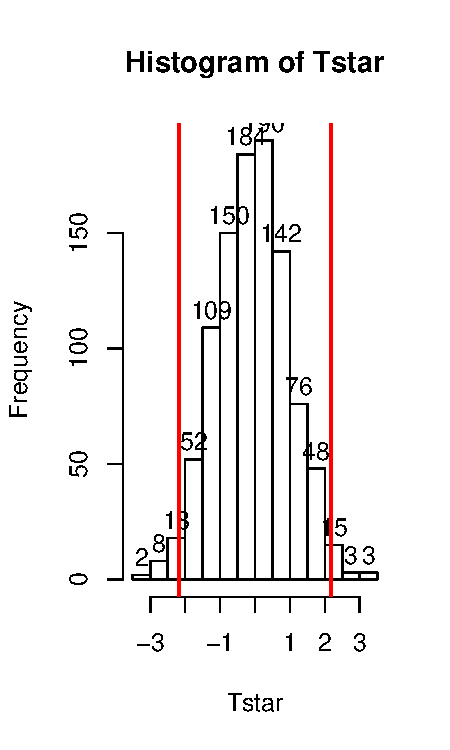
\includegraphics{02-reintroductionToStatistics_files/figure-latex/Figure2-12-1.pdf}
\caption{\label{fig:Figure2-12}Permutation distribution of the \(t\)-statistic}
\end{figure}

The parametric version of these results is based on using what is called
the \textbf{\emph{two-independent sample t-test}}. There are actually
two versions of this test, one that assumes that variances are equal in
the groups and one that does not. There is a rule of thumb that if the
\textbf{ratio of the larger standard deviation over the smaller standard
deviation is less than 2, the equal variance procedure is OK}. It ends
up that this assumption is less important if the sample sizes in the
groups are approximately equal and more important if the groups contain
different numbers of observations. In comparing the two potential test
statistics, the procedure that assumes equal variances has a complicated
denominator (see the formula above for \(t\) involving \(s_p\)) but a
simple formula for \textbf{\emph{degrees of freedom}}
(\textbf{\emph{df}}) for the \(t\)-distribution (\(df=n_1+n_2-2\)) that
approximates the distribution of the test statistic, \(t\), under the
null hypothesis. The procedure that assumes unequal variances has a
simpler test statistic and a very complicated degrees of freedom
formula. The equal variance procedure is most similar to the ANOVA
methods we will consider in Chapters 2 and 3 so that will be our focus
for the two group problem. Fortunately, both of these methods are
readily available in the \texttt{t.test} function in R if needed.

If the assumptions for the equal variance \(t\)-test are met and the
null hypothesis is true, then the sampling distribution of the test
statistic should follow a \(t\)-distribution with \(n_1+n_2-2\) degrees
of freedom. The \textbf{\emph{t-distribution}} is a bell-shaped curve
that is more spread out for smaller values of degrees of freedom as
shown in Figure \ref{fig:Figure2-13}. The \(t\)-distribution looks more
and more like a \textbf{\emph{standard normal distribution}}
(\(N(0,1)\)) as the degrees of freedom increase.



\begin{figure}
\centering
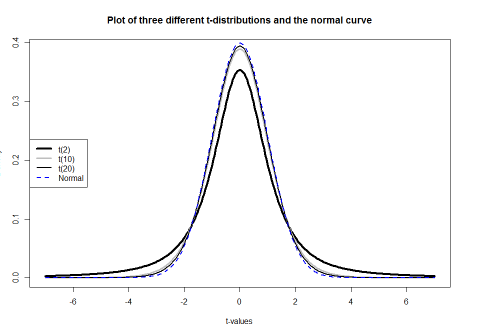
\includegraphics{chapter1_files/image045small.png}
\caption{\label{fig:Figure2-13}Plots of \(t\) and normal distributions}
\end{figure}

To get the p-value for the parametric \(t\)-test, we need to calculate
the test statistic and \(df\), then look up the areas in the tails of
the \(t\)-distribution relative to the observed \(t\)-statistic. We'll
learn how to use R to do this below, but for now we will allow the
\texttt{t.test} function to take care of this for us. The
\texttt{t.test} function uses our formula notation
(\texttt{Years\ \textasciitilde{}\ Attr}) and then \texttt{data=...} as
we saw before for making plots. To get the equal-variance test result,
the \texttt{var.equal=T} option needs to be turned on. Then
\texttt{t.test} provides us with lots of useful output. The three
results we've been discussing are highlighted in the output below -- the
test statistic value (-2.17), \(df=73\), and the p-value, from the
\(t\)-distribution with 73 degrees of freedom, of 0.033.

\begin{Shaded}
\begin{Highlighting}[]
\KeywordTok{t.test}\NormalTok{(Years }\OperatorTok{~}\StringTok{ }\NormalTok{Attr, }\DataTypeTok{data=}\NormalTok{MockJury2, }\DataTypeTok{var.equal=}\NormalTok{T)}
\end{Highlighting}
\end{Shaded}

\begin{verbatim}
## 
##  Two Sample t-test
## 
## data:  Years by Attr
## t = -2.1702, df = 73, p-value = 0.03324
## alternative hypothesis: true difference in means is not equal to 0
## 95 percent confidence interval:
##  -3.5242237 -0.1500295
## sample estimates:
##      mean in group Average mean in group Unattractive 
##                   3.973684                   5.810811
\end{verbatim}

So the parametric \(t\)-test gives a p-value of 0.033 from a test
statistic of -2.1702. The negative sign on the test statistic occurred
because the function took \emph{Average} - \emph{Unattractive} which is
the opposite direction as \texttt{diffmean}. The p-value is very similar
to the two permutation results found before. The reason for this
similarity is that the permutation distribution with 73 degrees of
freedom. Figure \ref{fig:Figure2-14} shows how similar the two
distributions happened to be here.



\begin{figure}
\centering
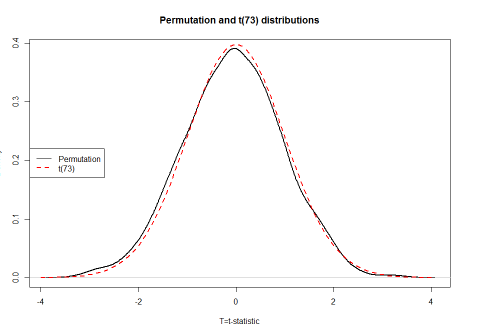
\includegraphics{chapter1_files/image047small.png}
\caption{\label{fig:Figure2-14}Plot of permutation and \(t\) distribution with \(df=73\).}
\end{figure}

In your previous statistics course, you might have used an applet or a
table to find p-values such as what was provided in the previous R
output. When not directly provided in the output of a function, R can be
used to look up p-values\footnote{On exams, you will be asked to
  describe the area of interest, sketch a picture of the area of
  interest, and/or note the distribution you would use.} from named
distributions such as the \(t\)-distribution. In this case, the
distribution of the test statistic under the null hypothesis is a
\(t(73)\) or a \(t\) with 73 degrees of freedom. The \texttt{pt}
function is used to get p-values from the \(t\)-distribution in the same
manner that \texttt{pdata} could help us to find p-values from the
permutation distribution. We need to provide the \texttt{df=...} and
specify the tail of the distribution of interest using the
\texttt{lower.tail} option along with the cutoff of interest. If we want
the area to the left of -2.17:

\begin{Shaded}
\begin{Highlighting}[]
\KeywordTok{pt}\NormalTok{(}\OperatorTok{-}\FloatTok{2.1702}\NormalTok{, }\DataTypeTok{df=}\DecValTok{73}\NormalTok{, }\DataTypeTok{lower.tail=}\NormalTok{T)}
\end{Highlighting}
\end{Shaded}

\begin{verbatim}
## [1] 0.01662286
\end{verbatim}

And we can double it to get the p-value that \texttt{t.test} provided
earlier, because the \(t\)-distribution is symmetric:

\begin{Shaded}
\begin{Highlighting}[]
\DecValTok{2}\OperatorTok{*}\KeywordTok{pt}\NormalTok{(}\OperatorTok{-}\FloatTok{2.1702}\NormalTok{, }\DataTypeTok{df=}\DecValTok{73}\NormalTok{, }\DataTypeTok{lower.tail=}\NormalTok{T)}
\end{Highlighting}
\end{Shaded}

\begin{verbatim}
## [1] 0.03324571
\end{verbatim}

More generally, we could always make the test statistic positive using
the absolute value, find the area to the right of it, and then double
that for a two-sided test p-value:

\begin{Shaded}
\begin{Highlighting}[]
\DecValTok{2}\OperatorTok{*}\KeywordTok{pt}\NormalTok{(}\KeywordTok{abs}\NormalTok{(}\OperatorTok{-}\FloatTok{2.1702}\NormalTok{), }\DataTypeTok{df=}\DecValTok{73}\NormalTok{, }\DataTypeTok{lower.tail=}\NormalTok{T)}
\end{Highlighting}
\end{Shaded}

\begin{verbatim}
## [1] 1.966754
\end{verbatim}

Permutation distributions do not need to match the named parametric
distribution to work correctly, although this happened in the previous
example. The parametric certain conditions to be met for the sampling
distribution of the statistic to follow the named distribution and
provide accurate p-values. The conditions for the equal variance t-test
are:

\newpage

\begin{enumerate}
\def\labelenumi{\arabic{enumi}.}
\item
  \textbf{Independent observations}: Each observation obtained is
  unrelated to all other observations. To assess this, consider whether
  anything in the data collection might lead to clustered or related
  observations that are un-related to the differences in the groups. For
  example, was the same person measured more than once?\footnote{In some
    studies, the same subject might be measured in both conditions and
    this violates the assumptions of this procedure.}
\item
  \textbf{Equal variances} in the groups (because we used a procedure
  that assumes equal variances! -- there is another procedure that
  allows you to relax this assumption if needed\ldots{}). To assess
  this, compare the standard deviations and variability in the beanplots
  and see if they look noticeably different. Be particularly critical of
  this assessment if the sample sizes differ greatly between groups.
\item
  \textbf{Normal distributions} of the observations in each group. We'll
  learn more diagnostics later, but the boxplots and beanplots are a
  good place to start to help you look for skews or outliers, which were
  both present here. If you find skew and/or outliers, that would
  suggest a problem with the assumption of normality as normal
  distributions are symmetric and extreme observations occur very
  rarely.
\end{enumerate}

For the permutation test, we relax the third condition and replace it
with:

\begin{enumerate}
\def\labelenumi{\arabic{enumi}.}
\setcounter{enumi}{2}
\tightlist
\item
  \textbf{\emph{Similar distributions between the groups:}} The
  permutation approach allows valid inferences as long as the two groups
  have similar shapes and only possibly differ in their centers. In
  other words, the distributions need not look normal for the procedure
  to work well, but they do need to look similar.
\end{enumerate}

In the prisoner ``juror'' study, we can assume that the independent
observation condition is met because there is no information suggesting
that the same subjects were measured more than once or that some other
type of grouping in the responses was present (like the subjects were
divided in groups and placed in rooms to discuss their responses prior
to submitting them). The equal variance condition might be violated. The
variances need not be equal as the procedure can still provide
reasonable results with some violation of this assumption. The standard
deviations are 2.8 vs 4.4, so this difference is not ``large'' according
to the rule of thumb noted above. It is, however, close to being
considered problematic. It would be difficult to reasonably assume that
the normality condition is met here (Figure \ref{fig:Figure2-6} with
clear right skews in both groups and potential outliers which causes
concerns for (3) for the parametric procedure. The shapes look similar
for the two groups so there is less reason to be concerned with using
the permutation approach based on its version of (3) above.

The permutation approach is resistant to impacts of violations of the
normality assumption. It is not resistant to impact of violations of any
of the other assumptions. In fact, it can be quite sensitive to unequal
variances as it will detect differences in the variances of the groups
instead of differences in the means. Its scope of inference is the same
as the parametric approach and can lead to similarly inaccurate
conclusions in the presence of non-independent observations as for the
parametric approach. In this example, we discover that parametric and
permutation approaches provide very similar inferences.

\section{Second example of permutation tests}\label{section2-7}

In every chapter, we will follow the first example used to motivate and
explain the methods with a ``worked'' example where we focus just on the
results. In a previous semester, some of the STAT 217 students (
\textbf{\emph{n}}=79) provided information on their \emph{Sex},
\emph{Age}, and current cumulative \emph{GPA}. We might be interested in
whether Males and Females had different average GPAs. First, we can take
a look at the difference in the responses by groups based on the output
and as displayed in Figure \ref{fig:Figure2-15}.

\begin{Shaded}
\begin{Highlighting}[]
\NormalTok{s217 <-}\StringTok{ }\KeywordTok{read.csv}\NormalTok{(}\StringTok{"http://www.math.montana.edu/courses/s217/documents/s217.csv"}\NormalTok{)}
\KeywordTok{require}\NormalTok{(mosaic)}
\KeywordTok{require}\NormalTok{(beanplot)}
\KeywordTok{mean}\NormalTok{(GPA}\OperatorTok{~}\NormalTok{Sex, }\DataTypeTok{data=}\NormalTok{s217)}
\end{Highlighting}
\end{Shaded}

\begin{verbatim}
##        F        M 
## 3.338378 3.088571
\end{verbatim}

\begin{Shaded}
\begin{Highlighting}[]
\KeywordTok{favstats}\NormalTok{(GPA}\OperatorTok{~}\NormalTok{Sex, }\DataTypeTok{data=}\NormalTok{s217)}
\end{Highlighting}
\end{Shaded}

\begin{verbatim}
##   Sex  min  Q1 median   Q3 max     mean        sd  n missing
## 1   F 2.50 3.1  3.400 3.70   4 3.338378 0.4074549 37       0
## 2   M 1.96 2.8  3.175 3.46   4 3.088571 0.4151789 42       0
\end{verbatim}




\begin{figure}
\centering
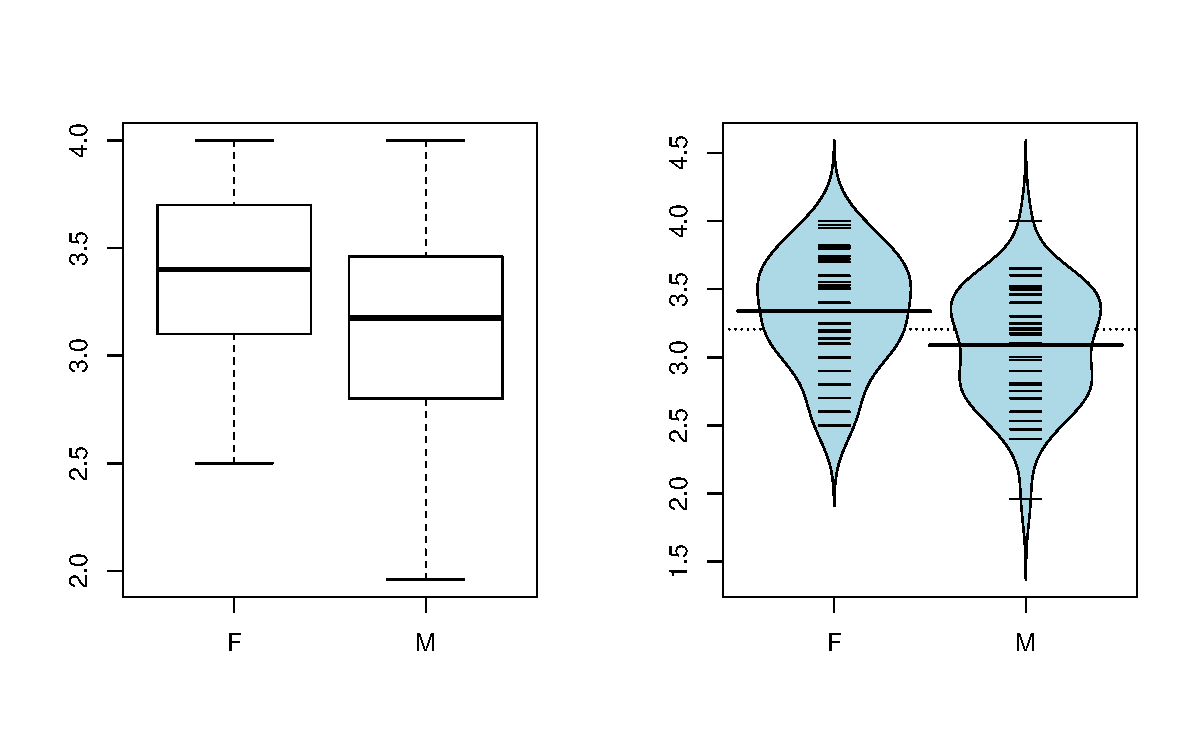
\includegraphics{02-reintroductionToStatistics_files/figure-latex/Figure2-15-1.pdf}
\caption{\label{fig:Figure2-15}Side-by-side boxplot and beanplot of GPAs of STAT 217
students by sex.}
\end{figure}

\begin{Shaded}
\begin{Highlighting}[]
\KeywordTok{par}\NormalTok{(}\DataTypeTok{mfrow=}\KeywordTok{c}\NormalTok{(}\DecValTok{1}\NormalTok{,}\DecValTok{2}\NormalTok{))}
\KeywordTok{boxplot}\NormalTok{(GPA}\OperatorTok{~}\NormalTok{Sex, }\DataTypeTok{data=}\NormalTok{s217)}
\KeywordTok{beanplot}\NormalTok{(GPA}\OperatorTok{~}\NormalTok{Sex, }\DataTypeTok{data=}\NormalTok{s217, }\DataTypeTok{log=}\StringTok{""}\NormalTok{, }\DataTypeTok{col=}\StringTok{"lightblue"}\NormalTok{, }\DataTypeTok{method=}\StringTok{"jitter"}\NormalTok{)}
\end{Highlighting}
\end{Shaded}

In these data, the distributions of the GPAs look to be left skewed but
maybe not as dramatically as the responses were right-skewed in the
previous example. The Female GPAs look to be slightly higher than for
Males (0.25 GPA difference in the means) but is that a ``real''
difference? We need our inference tools to more fully assess these
differences.

\begin{Shaded}
\begin{Highlighting}[]
\KeywordTok{diffmean}\NormalTok{(GPA}\OperatorTok{~}\NormalTok{Sex, }\DataTypeTok{data=}\NormalTok{s217)}
\end{Highlighting}
\end{Shaded}

\begin{verbatim}
##   diffmean 
## -0.2498069
\end{verbatim}

First, we can try the parametric approach:

\begin{Shaded}
\begin{Highlighting}[]
\KeywordTok{t.test}\NormalTok{(GPA}\OperatorTok{~}\NormalTok{Sex, }\DataTypeTok{data=}\NormalTok{s217, }\DataTypeTok{var.equal=}\NormalTok{T)}
\end{Highlighting}
\end{Shaded}

\begin{verbatim}
## 
##  Two Sample t-test
## 
## data:  GPA by Sex
## t = 2.6919, df = 77, p-value = 0.008713
## alternative hypothesis: true difference in means is not equal to 0
## 95 percent confidence interval:
##  0.06501838 0.43459552
## sample estimates:
## mean in group F mean in group M 
##        3.338378        3.088571
\end{verbatim}

So the test statistic was observed to be \(t=2.69\) and it hopefully
follows a \(t(77)\) distribution under the null hypothesis. This
provides a p-value of 0.008713 that we can trust if all the conditions
to use this procedure are met. Compare these results to the permutation
approach, which relaxes that normality assumption, with the results that
follow. In the permutation test, \(T=2.692\) and the p-value is 0.005
which is a little smaller than the result provided by the parametric
approach. The agreement of the two approaches, again, provides some
re-assurance about the use of either approach.

\begin{Shaded}
\begin{Highlighting}[]
\NormalTok{Tobs <-}\StringTok{ }\KeywordTok{t.test}\NormalTok{(GPA}\OperatorTok{~}\NormalTok{Sex, }\DataTypeTok{data=}\NormalTok{s217, }\DataTypeTok{var.equal=}\NormalTok{T)}\OperatorTok{$}\NormalTok{statistic}
\NormalTok{Tstar <-}\StringTok{ }\KeywordTok{matrix}\NormalTok{(}\OtherTok{NA}\NormalTok{, }\DataTypeTok{nrow=}\NormalTok{B)}
\ControlFlowTok{for}\NormalTok{ (b }\ControlFlowTok{in}\NormalTok{ (}\DecValTok{1}\OperatorTok{:}\NormalTok{B))\{}
\NormalTok{  Tstar[b] <-}\StringTok{ }\KeywordTok{t.test}\NormalTok{(GPA}\OperatorTok{~}\KeywordTok{shuffle}\NormalTok{(Sex), }\DataTypeTok{data=}\NormalTok{s217, }\DataTypeTok{var.equal=}\NormalTok{T)}\OperatorTok{$}\NormalTok{statistic}
\NormalTok{\}}
\KeywordTok{pdata}\NormalTok{(}\KeywordTok{abs}\NormalTok{(Tstar),}\KeywordTok{abs}\NormalTok{(Tobs),}\DataTypeTok{lower.tail=}\NormalTok{F)}
\end{Highlighting}
\end{Shaded}




\begin{figure}
\centering
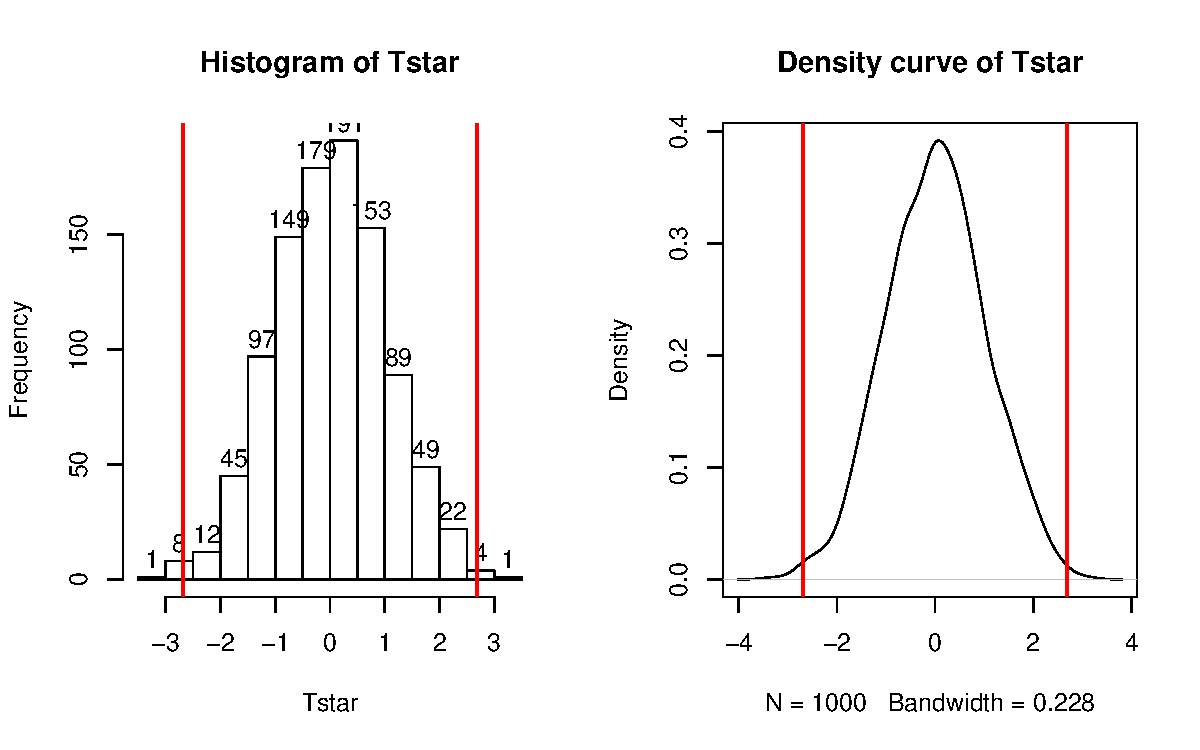
\includegraphics{02-reintroductionToStatistics_files/figure-latex/Figure2-16-1.pdf}
\caption{\label{fig:Figure2-16}Histogram and density curve of permutation distribution of
test statistic for STAT 217 GPAs.}
\end{figure}

\begin{Shaded}
\begin{Highlighting}[]
\KeywordTok{par}\NormalTok{(}\DataTypeTok{mfrow=}\KeywordTok{c}\NormalTok{(}\DecValTok{1}\NormalTok{,}\DecValTok{2}\NormalTok{))}
\KeywordTok{hist}\NormalTok{(Tstar,}\DataTypeTok{labels=}\NormalTok{T)}
\KeywordTok{abline}\NormalTok{(}\DataTypeTok{v=}\KeywordTok{c}\NormalTok{(}\OperatorTok{-}\DecValTok{1}\NormalTok{,}\DecValTok{1}\NormalTok{)}\OperatorTok{*}\NormalTok{Tobs, }\DataTypeTok{lwd=}\DecValTok{2}\NormalTok{, }\DataTypeTok{col=}\StringTok{"red"}\NormalTok{)}
\KeywordTok{plot}\NormalTok{(}\KeywordTok{density}\NormalTok{(Tstar), }\DataTypeTok{main=}\StringTok{"Density curve of Tstar"}\NormalTok{)}
\KeywordTok{abline}\NormalTok{(}\DataTypeTok{v=}\KeywordTok{c}\NormalTok{(}\OperatorTok{-}\DecValTok{1}\NormalTok{,}\DecValTok{1}\NormalTok{)}\OperatorTok{*}\NormalTok{Tobs, }\DataTypeTok{lwd=}\DecValTok{2}\NormalTok{, }\DataTypeTok{col=}\StringTok{"red"}\NormalTok{)}
\end{Highlighting}
\end{Shaded}

Here is a full write-up of the results using all 6+ hypothesis testing
steps, using the permutation results:

\begin{enumerate}
\def\labelenumi{\arabic{enumi}.}
\setcounter{enumi}{-1}
\item
  \emph{Isolate the claim to be proved and method to use (define a test
  statistic T)} We want to test for a difference in the means between
  males and females and will use the equal-variance two-sample t-test
  statistic to compare them, making a decision at the 5\% significance
  level.
\item
  Write the null and alternative hypotheses

  \begin{itemize}
  \item
    \(H_0: \mu_{male} = \mu_{female}\)

    \begin{itemize}
    \tightlist
    \item
      where \(\mu_{male}\) is the true mean GPA for males and
      \(\mu_{female}\) is true mean GPA for females.
    \end{itemize}
  \item
    \(H_A: \mu_{male} \ne \mu_{female}\)
  \end{itemize}
\item
  Check conditions for the procedure being used

  \begin{itemize}
  \item
    \textbf{Independent observations condition}: It appears that this
    assumption is met because there is no reason to assume any
    clustering or grouping of responses that might create dependence in
    the observations. The only possible consideration is that the
    observations were taken from different sections and there could be
    some differences between the sections. However, for overall GPA this
    not likely to be a big issue. The only way this could create a
    violation here is if certain sections tended to attract students
    with different GPA levels (such as the 9 am section had the
    best/worst GPA students\ldots{}).
  \item
    \textbf{Equal variance condition} : There is a small difference in
    the range of the observations in the two groups but the standard
    deviations are very similar so there is no evidence that this
    condition is violated.
  \item
    \textbf{Similar distribution condition}: Based on the side-by-side
    boxplots and beanplots, it appears that both groups have slightly
    left-skewed distributions, which could be problematic for the
    parametric approach, but the permutation approach condition is not
    violated since the distributions look to have fairly similar shapes.
  \end{itemize}
\item
  Find the value of the appropriate test statistic

  \begin{itemize}
  \tightlist
  \item
    \(T=2.69\) from the previous R output.
  \end{itemize}
\item
  Find the p-value

  \begin{itemize}
  \item
    p-value=0.005 from the permutation distribution results.
  \item
    This means that there is about a 0.5\% chance we would observe a
    difference in mean GPA (female-male or male-female) of 0.25 points
    or more if there in fact no difference in true mean GPA between
    females and males in STAT 217 in a particular semester.
  \end{itemize}
\end{enumerate}

\newpage

\begin{enumerate}
\def\labelenumi{\arabic{enumi}.}
\setcounter{enumi}{4}
\item
  Decision

  \begin{itemize}
  \tightlist
  \item
    Since the p-value is ``small'' (\emph{a priori} 5\% significance
    level selected), we can reject the null hypothesis.
  \end{itemize}
\item
  Conclusion and scope of inference, specific to the problem

  \begin{itemize}
  \item
    There is strong evidence against the null hypothesis of no
    difference in the true mean GPA between males and females for the
    STAT 217 students in this semester and so we conclude that there is
    evidence of a difference in the mean GPAs between males and females
    in STAT 217 students.
  \item
    Because this was not a randomized experiment, we can't say that the
    difference in sex causes the difference in mean GPA and because it
    was not a random sample from a larger population, our inferences
    only pertain the STAT 217 students that responded to the survey in
    that semester.
  \end{itemize}
\end{enumerate}

\section{Confidence intervals and bootstrapping}\label{section2-8}

Randomly shuffling the treatments between the observations is like
randomly sampling the treatments without replacement. In other words, we
randomly sample one observation at a observations. This provides us with
a technique for testing hypotheses because it provides new splits of the
observations into groups that are as interesting as what we observed if
the null hypothesis is assumed true. In most situations, we also want to
estimate parameters of interest and provide \textbf{\emph{confidence
intervals}} for those parameters (an interval where we are \_\_\%
\textbf{\emph{confident}} that the true parameter lies). As before,
there are two options we will consider -- a parametric and a
nonparametric approach. The nonparametric approach will be using what is
called \textbf{\emph{bootstrapping}} and draws its name from ``pull
yourself up by your bootstraps'' where you improve your situation based
on your own efforts. In statistics, we make our situation or inferences
better by re-using the observations we have by assuming that the sample
represents the population. Since each observation represents other
similar observations in the population that we didn't get to measure, if
we \textbf{\emph{sample with replacement}} to generate a new data set of
size \emph{n} from our data set (also of size \emph{n}) it mimics the
process of taking our population of interest. This process also ends up
giving us useful sampling distributions of statistics even when our
standard normality assumption is violated, similar to what we
encountered in the permutation tests. Bootstrapping is especially useful
in situations where we are interested in statistics other than the mean
(say we want a confidence interval for a median or a standard deviation)
or when we consider functions of more than one parameter and don't want
to derive the distribution of the statistic (say the difference in two
medians). In this text, bootstrapping is used to provide more
trustworthy inferences when some of our assumptions (especially
normality) might be violated for our parametric procedure.

To perform bootstrapping, we will use the \texttt{resample} function
from the \texttt{mosaic} package. We can apply this function to a data
set and get a new version of the data set by sampling new observations
\emph{with replacement} from the original one. The new, bootstrapped
version of the data set (called \texttt{MockJury\_BTS} below) contains a
new variable called \texttt{orig.\ id} which is the number of the
subject from the original data set. By summarizing how often each of
these id's occurred in a bootstrapped data set, we can see how the
re-sampling works. The \texttt{table} function will count up how many
times each observation was used in the bootstrap sample, providing a row
with the id followed by a row with the count\footnote{The
  \texttt{as.numeric} function is also used here. It really isn't
  important but makes sure the output of \texttt{table} is sorted by
  observation number by first converting the \emph{orig.id} variable
  into a numeric vector.}. In the first bootstrap sample shown, the 2nd,
7th, and 9th observations were sampled one time each, the 4th
observation was sampled three times, and the 1st, 3rd, 5th, and many
others were not sampled at all. Bootstrap sampling thus picks some
observations multiple times and to do that it has to ignore some
observations.

\newpage

\begin{Shaded}
\begin{Highlighting}[]
\NormalTok{MockJury_BTS <-}\StringTok{ }\KeywordTok{resample}\NormalTok{(MockJury2)}
\KeywordTok{table}\NormalTok{(}\KeywordTok{as.numeric}\NormalTok{(MockJury_BTS}\OperatorTok{$}\NormalTok{orig.id))}
\end{Highlighting}
\end{Shaded}

\begin{verbatim}
## 
##  1  2  3  4  5  6 10 11 12 14 15 17 18 19 20 22 24 26 29 30 32 35 36 37 39 
##  1  2  2  1  3  2  1  2  1  1  3  1  2  1  2  1  2  1  2  2  2  2  1  2  2 
## 40 42 43 44 45 46 47 48 49 55 58 59 60 61 69 70 71 72 74 75 
##  2  1  1  4  2  2  1  2  1  2  1  1  2  2  2  2  2  1  1  1
\end{verbatim}

Like in permutations, one randomization isn't enough. A second bootstrap
sample is also provided to help you get a sense of what it is doing to
generate a data set. It did not select subject 7 but did select 2, 4, 6,
and 8 two times. You can see other variations in the resulting
re-sampling of subjects with the most sampled subject being the chance
of selecting any observation for any slot in the new data set is
\(1/75\) and the expected or mean number of appearances we expect to see
for an observation is the number of tries times the probably of
selection on each so \(75*1/75=1\).

\begin{Shaded}
\begin{Highlighting}[]
\NormalTok{MockJury_BTS2 <-}\StringTok{ }\KeywordTok{resample}\NormalTok{(MockJury2)}
\KeywordTok{table}\NormalTok{(}\KeywordTok{as.numeric}\NormalTok{(MockJury_BTS2}\OperatorTok{$}\NormalTok{orig.id))}
\end{Highlighting}
\end{Shaded}

\begin{verbatim}
## 
##  1  2  3  5  6  8 11 12 13 14 15 18 19 20 21 23 24 26 27 28 29 31 32 34 36 
##  1  1  1  1  4  1  1  1  1  3  1  1  1  1  3  2  2  1  1  1  2  1  2  1  2 
## 37 38 40 42 46 48 50 51 52 56 58 59 61 62 63 66 67 68 69 72 73 74 75 
##  1  2  1  1  1  2  4  1  1  1  3  2  1  1  1  1  1  1  2  3  1  4  2
\end{verbatim}

We can use the two results to get an idea of distribution of results in
terms of number of times observations might be re-sampled when sampling
with replacement and the variation in those results, as shown in Figure
\ref{fig:Figure2-17}. We could also derive the expected counts for each
number of times of re-sampling when we start with all observations
having an equal chance and sampling with replacement but this isn't
important for using bootstrapping methods.




\begin{figure}
\centering
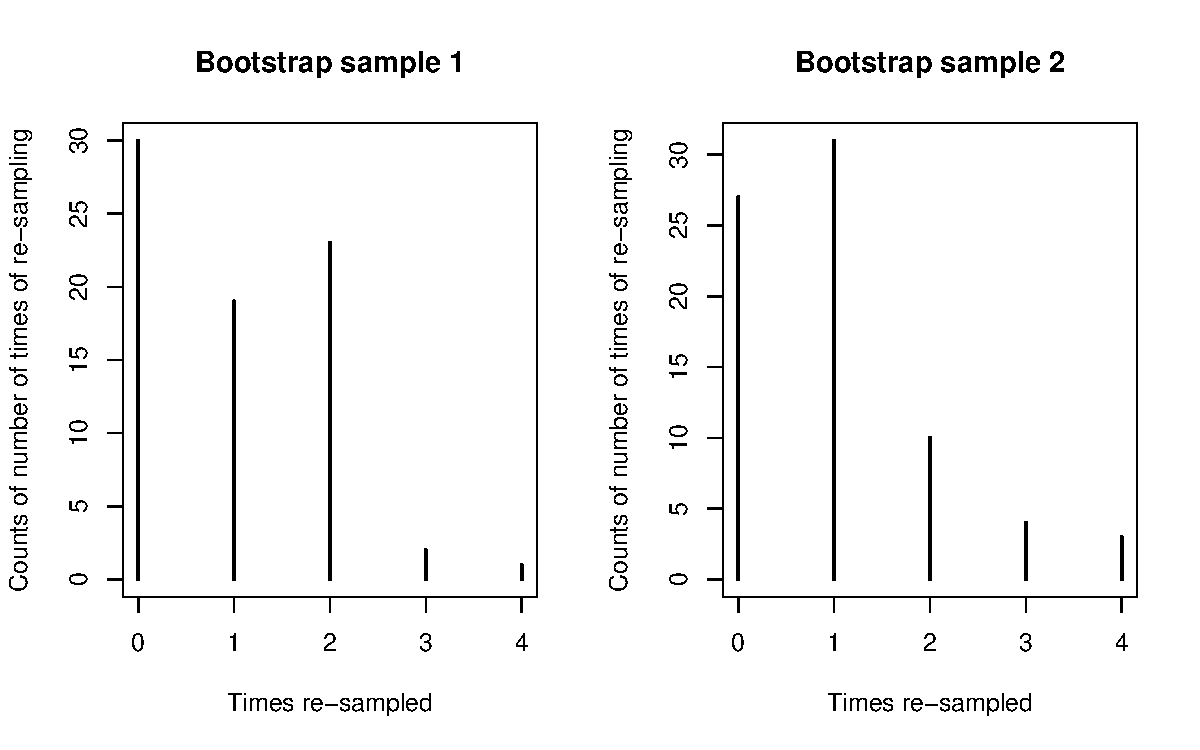
\includegraphics{02-reintroductionToStatistics_files/figure-latex/Figure2-17-1.pdf}
\caption{\label{fig:Figure2-17}Counts of number of times of observation (or not observed
for times re-sampled of 0) for two bootstrap samples.}
\end{figure}

The main point of this exploration was to see that each run of the
\texttt{resample} function provides a new version of the data set.
Repeating this \(B\) times using another \texttt{for} loop, we will
track our quantity of interest, say \(T\), in all these new ``data
sets'' and call those results \(T^*\). The distribution of the
bootstrapped \(T^*\) statistics will tell us about the range of results
to expect for the statistic and the middle \_\_\% of the \(T^*\)'s
provides a \textbf{\emph{bootstrap confidence interval}}\footnote{There
  are actually many ways to use this information to make a confidence
  interval. We are using the simplest method that is called the
  ``percentile'' method.} for the true parameter -- here the
\emph{difference in the two population means}.

To make this concrete, we can revisit our previous examples, starting
with the \texttt{MockJury2} data created before and our interest in
comparing the mean sentences for the \emph{Average}and
\emph{Unattractive} picture groups. The bootstrapping code is very
similar to the permutation code except that we apply the
\texttt{resample} function to the entire data set as opposed to the
\texttt{shuffle} function being applied to the explanatory variable.

\begin{Shaded}
\begin{Highlighting}[]
\KeywordTok{par}\NormalTok{(}\DataTypeTok{mfrow=}\KeywordTok{c}\NormalTok{(}\DecValTok{1}\NormalTok{,}\DecValTok{2}\NormalTok{))}
\NormalTok{Tobs <-}\StringTok{ }\KeywordTok{diffmean}\NormalTok{(Years }\OperatorTok{~}\StringTok{ }\NormalTok{Attr, }\DataTypeTok{data=}\NormalTok{MockJury2); Tobs}
\end{Highlighting}
\end{Shaded}

\begin{verbatim}
## diffmean 
## 1.837127
\end{verbatim}

\begin{Shaded}
\begin{Highlighting}[]
\NormalTok{B <-}\StringTok{ }\DecValTok{1000}
\NormalTok{Tstar <-}\StringTok{ }\KeywordTok{matrix}\NormalTok{(}\OtherTok{NA}\NormalTok{,}\DataTypeTok{nrow=}\NormalTok{B)}
\ControlFlowTok{for}\NormalTok{ (b }\ControlFlowTok{in}\NormalTok{ (}\DecValTok{1}\OperatorTok{:}\NormalTok{B))\{}
\NormalTok{  Tstar[b] <-}\StringTok{ }\KeywordTok{diffmean}\NormalTok{(Years }\OperatorTok{~}\StringTok{ }\NormalTok{Attr, }\DataTypeTok{data=}\KeywordTok{resample}\NormalTok{(MockJury2))}
\NormalTok{  \}}
\KeywordTok{favstats}\NormalTok{(Tstar)}
\end{Highlighting}
\end{Shaded}

\begin{verbatim}
##         min       Q1   median       Q3      max     mean        sd    n
##  -0.3627312 1.305773 1.833091 2.385281 4.988756 1.854428 0.8438987 1000
##  missing
##        0
\end{verbatim}





\begin{figure}
\centering
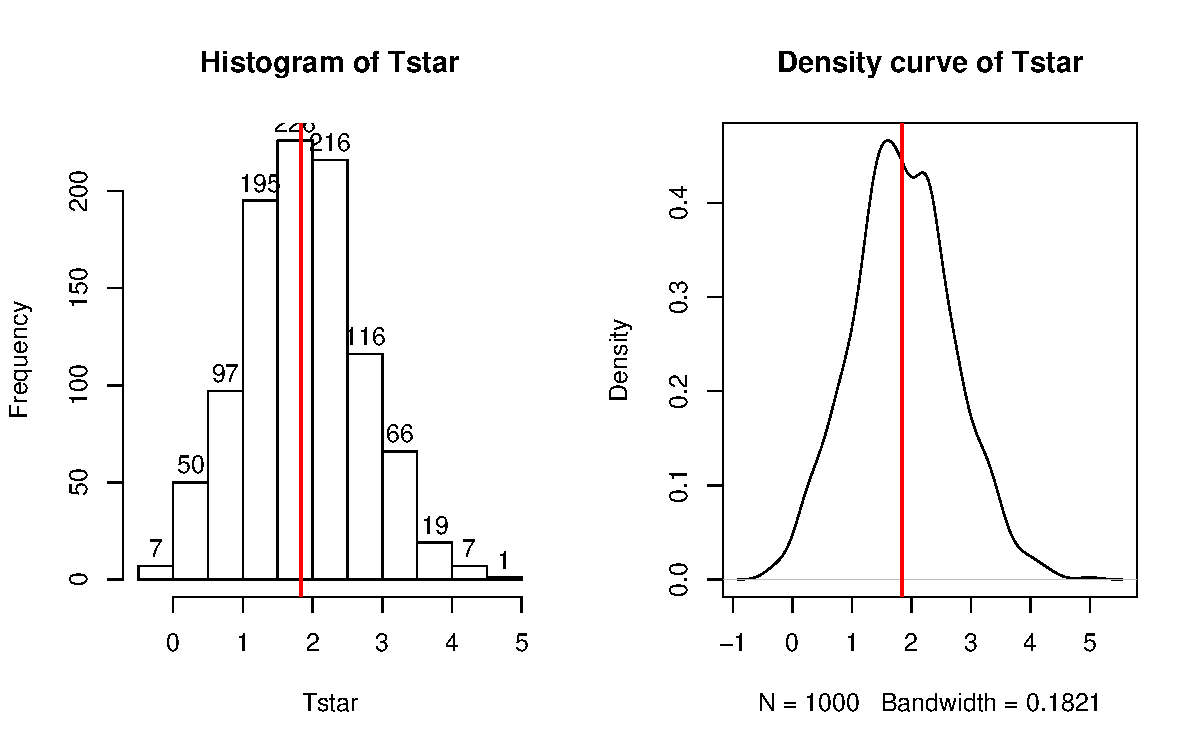
\includegraphics{02-reintroductionToStatistics_files/figure-latex/Figure2-18-1.pdf}
\caption{\label{fig:Figure2-18}Histogram and density curve of bootstrap distributions of
difference in sample mean \texttt{Years} with vertical line for the
observed difference in the means of 1.84 years.}
\end{figure}

\begin{Shaded}
\begin{Highlighting}[]
\KeywordTok{hist}\NormalTok{(Tstar, }\DataTypeTok{labels=}\NormalTok{T)}
\KeywordTok{abline}\NormalTok{(}\DataTypeTok{v=}\NormalTok{Tobs, }\DataTypeTok{col=}\StringTok{"red"}\NormalTok{, }\DataTypeTok{lwd=}\DecValTok{2}\NormalTok{)}
\KeywordTok{plot}\NormalTok{(}\KeywordTok{density}\NormalTok{(Tstar), }\DataTypeTok{main=}\StringTok{"Density curve of Tstar"}\NormalTok{)}
\KeywordTok{abline}\NormalTok{(}\DataTypeTok{v=}\NormalTok{Tobs, }\DataTypeTok{col=}\StringTok{"red"}\NormalTok{, }\DataTypeTok{lwd=}\DecValTok{2}\NormalTok{)}
\end{Highlighting}
\end{Shaded}

In this situation, the observed difference in the mean sentences is 1.84
years (Unattractive-Average), which is the vertical line in Figure
\ref{fig:Figure2-18}. The bootstrap distribution shows the results for
the difference in the sample means when fake data sets are
re-constructed by sampling from the data set with replacement. The
bootstrap distribution is approximately centered at the observed value
(difference in the sample means) and is relatively symmetric.

The permutation distribution in the same situation (Figure
\ref{fig:Figure2-12}) had a similar shape but was centered at 0.
Permutations create sampling distributions based on assuming the null
hypothesis is true, which is useful for hypothesis testing.
Bootstrapping creates distributions centered at the observed result,
which is the sampling distribution ``under the alternative'' or when no
null hypothesis is assumed; bootstrap distributions are useful for
generating confidence intervals for the true parameter values.

To create a 95\% bootstrap confidence interval for the difference in the
true mean sentences (\(\mu_{Unattr}-\mu_{Avg}\)), select the middle 95\%
of results from the bootstrap distribution. Specifically, find the 2.5th
percentile and the 97.5th percentile (values that put 2.5 and 97.5\% of
the results to the left) in the bootstrap distribution, which leaves
95\% in the middle for the confidence interval. To find percentiles in a
distribution in R, functions are of the form
\texttt{q{[}Name\ of\ distribution{]}}, with the function \texttt{qt}
extracting percentiles from a \(t\)-distribution (examples below). From
the bootstrap results, use the \texttt{qdata} function on the
\texttt{Tstar} results that contain the bootstrap distribution of the
statistic of interest.

\begin{Shaded}
\begin{Highlighting}[]
\KeywordTok{qdata}\NormalTok{(Tstar, }\FloatTok{0.025}\NormalTok{)}
\end{Highlighting}
\end{Shaded}

\begin{verbatim}
##         p  quantile 
## 0.0250000 0.2414232
\end{verbatim}

\begin{Shaded}
\begin{Highlighting}[]
\KeywordTok{qdata}\NormalTok{(Tstar, }\FloatTok{0.975}\NormalTok{)}
\end{Highlighting}
\end{Shaded}

\begin{verbatim}
##        p quantile 
## 0.975000 3.521528
\end{verbatim}

These results tell us that the 2.5th percentile of the bootstrap
distribution is at 0.26 years and the 97.5th percentile is at 3.50
years. We can combine these results to provide a 95\% confidence for
\(\mu_{Unattr}-\mu_{Avg}\) that is between 0.26 and 3.50. We can
interpret this as with any confidence interval, that we are 95\%
confident that the difference in the true mean suggested sentences
(Unattractive minus Average group) is between 0.26 and 3.50 years. We
can also obtain both percentiles in one line of code using:

\begin{Shaded}
\begin{Highlighting}[]
\NormalTok{quantiles <-}\StringTok{ }\KeywordTok{qdata}\NormalTok{(Tstar, }\KeywordTok{c}\NormalTok{(}\FloatTok{0.025}\NormalTok{,}\FloatTok{0.975}\NormalTok{))}
\NormalTok{quantiles}
\end{Highlighting}
\end{Shaded}

\begin{verbatim}
##        quantile     p
## 2.5%  0.2414232 0.025
## 97.5% 3.5215278 0.975
\end{verbatim}

Figure \ref{fig:Figure2-19} displays those same percentiles on the
bootstrap distribution residing in \texttt{Tstar}.




\begin{figure}
\centering
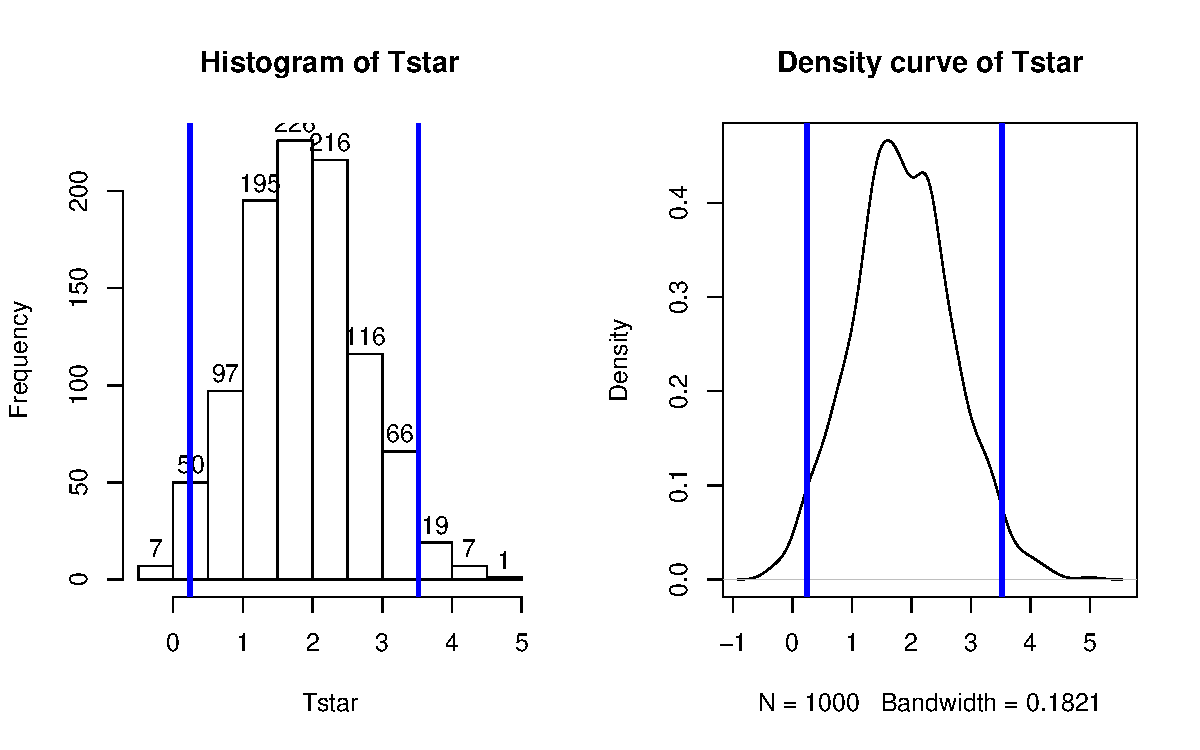
\includegraphics{02-reintroductionToStatistics_files/figure-latex/Figure2-19-1.pdf}
\caption{\label{fig:Figure2-19}Histogram and density curve of bootstrap distribution with
95\% bootstrap confidence intervals displayed (vertical lines).}
\end{figure}

\begin{Shaded}
\begin{Highlighting}[]
\KeywordTok{par}\NormalTok{(}\DataTypeTok{mfrow=}\KeywordTok{c}\NormalTok{(}\DecValTok{1}\NormalTok{,}\DecValTok{2}\NormalTok{))}
\KeywordTok{hist}\NormalTok{(Tstar, }\DataTypeTok{labels=}\NormalTok{T)}
\KeywordTok{abline}\NormalTok{(}\DataTypeTok{v=}\NormalTok{quantiles}\OperatorTok{$}\NormalTok{quantile, }\DataTypeTok{col=}\StringTok{"blue"}\NormalTok{, }\DataTypeTok{lwd=}\DecValTok{3}\NormalTok{)}
\KeywordTok{plot}\NormalTok{(}\KeywordTok{density}\NormalTok{(Tstar), }\DataTypeTok{main=}\StringTok{"Density curve of Tstar"}\NormalTok{)}
\KeywordTok{abline}\NormalTok{(}\DataTypeTok{v=}\NormalTok{quantiles}\OperatorTok{$}\NormalTok{quantile, }\DataTypeTok{col=}\StringTok{"blue"}\NormalTok{, }\DataTypeTok{lwd=}\DecValTok{3}\NormalTok{)}
\end{Highlighting}
\end{Shaded}

Although confidence intervals can exist without referencing hypotheses,
we can revisit our previous \(H_0: \mu_{Unattr} = \mu_{Avg}\). This null
hypothesis is equivalent to testing
\(H_0: \mu_{Unattr} - \mu_{Avg} = 0\), that the difference in the true
means is equal to 0 years. And the difference in the means was the scale
for our confidence interval, which did not contain 0 years. We will call
0 an interesting \textbf{\emph{reference value}} for the confidence
interval, because here it is the value where the true means are equal to
each other (have a difference of 0 years). In general, if our confidence
interval does not contain 0, then it is saying that 0 is not one of our
likely values for the difference in the true means. This implies that we
should reject a claim that they are equal. This provides the same
inferences for the hypotheses that we considered previously using both a
parametric and permutation approach.

The general summary is that we can use confidence intervals to test
hypotheses by assessing whether the reference value under the null
hypothesis is in the confidence interval (FTR \(H_0\)) or outside the
confidence interval (Reject \(H_0\)). P-values are more informative
about hypotheses but confidence intervals are more informative about the
size of differences, so both offer useful information and, as shown
here, can provide consistent conclusions about hypotheses.

As in the previous situation, we also want to consider the parametric
approach for comparison purposes and to have that method available,
especially to help us understand some methods where we will only
consider parametric inferences in later chapters. The parametric
confidence interval is called the \textbf{\emph{equal variance,
two-sample t confidence interval}} and assumes that the populations
being sampled from are normally distributed and leads to using a
\(t\)-distribution to form the interval. The output from the
\texttt{t.test} function provides the parametric 95\% confidence
interval calculated for you:

\begin{Shaded}
\begin{Highlighting}[]
\KeywordTok{t.test}\NormalTok{(Years }\OperatorTok{~}\StringTok{ }\NormalTok{Attr, }\DataTypeTok{data=}\NormalTok{MockJury2, }\DataTypeTok{var.equal=}\NormalTok{T)}
\end{Highlighting}
\end{Shaded}

\begin{verbatim}
## 
##  Two Sample t-test
## 
## data:  Years by Attr
## t = -2.1702, df = 73, p-value = 0.03324
## alternative hypothesis: true difference in means is not equal to 0
## 95 percent confidence interval:
##  -3.5242237 -0.1500295
## sample estimates:
##      mean in group Average mean in group Unattractive 
##                   3.973684                   5.810811
\end{verbatim}

The \texttt{t.test} function again switched the order of the groups and
provides slightly different end-points than our bootstrap confidence
interval (both are made at the 95\% confidence level though), which was
slightly narrower. Both intervals have the same interpretation, only the
methods for calculating the intervals and the assumptions differ.
Specifically, the bootstrap interval can tolerate different distribution
shapes other than normal and still provide intervals that work
well\footnote{When hypothesis tests ``work well'' they have high power
  to detect differences while having Type I error rates that are close
  to what we choose a priori. When confidence intervals ``work well'',
  they contain the true parameter value in repeated random samples at
  around the selected confidence level}. The other assumptions are all
the same as for the hypothesis test, where we continue to assume that we
have independent observations with equal variances for the two groups.

The formula that \texttt{t.test} is using to calculate the parametric
\textbf{\emph{equal-variance two-sample t confidence interval}} is:

\[\bar{x}_1 - \bar{x}_2 \mp t^*_{df}s_p\sqrt{\frac{1}{n_1}+\frac{1}{n_2}}\]

In this situation, the \emph{df} is again \(n_1+n_2-2\) and
\(s_p = \sqrt{\frac{(n_1-1)s_1^2 + (n_2-1)s_2^2}{n_1+n_2-2}}\). The
\(t^*_{df}\) is a multiplier that comes from finding the percentile from
the \(t\)-distribution that puts \(C\)\% in the middle of the
distribution with \(C\) being the confidence level. It is important to
note that this \(t^*\) has nothing to do with the previous test
statistic \(t\). It is confusing and many of you will, at some point,
happily take the result from a test statistic calculation and use it for
a multiplier in a \(t\)-based confidence interval. Figure
\ref{fig:Figure2-20} shows the \(t\)-distribution with 73 degrees of
freedom and the cut-offs that put 95\% of the area in the middle.




\begin{Shaded}
\begin{Highlighting}[]
\KeywordTok{par}\NormalTok{(}\DataTypeTok{mfrow=}\KeywordTok{c}\NormalTok{(}\DecValTok{1}\NormalTok{,}\DecValTok{1}\NormalTok{))}
\NormalTok{x<-}\KeywordTok{seq}\NormalTok{(}\DataTypeTok{from=}\OperatorTok{-}\DecValTok{4}\NormalTok{,}\DataTypeTok{to=}\DecValTok{4}\NormalTok{,}\DataTypeTok{length.out=}\DecValTok{200}\NormalTok{)}
\KeywordTok{plot}\NormalTok{(x,}\KeywordTok{dt}\NormalTok{(x,}\DataTypeTok{df=}\DecValTok{73}\NormalTok{),}\DataTypeTok{col=}\StringTok{"red"}\NormalTok{,}\DataTypeTok{lty=}\DecValTok{2}\NormalTok{,}\DataTypeTok{lwd=}\DecValTok{3}\NormalTok{,}\DataTypeTok{type=}\StringTok{"l"}\NormalTok{,}\DataTypeTok{xlab=}\StringTok{"t-values"}\NormalTok{,}\DataTypeTok{ylab=}\StringTok{"Density"}\NormalTok{,}
     \DataTypeTok{main=}\StringTok{"Plot of t(73) distribution"}\NormalTok{ )}
\KeywordTok{abline}\NormalTok{(}\DataTypeTok{v=}\OperatorTok{-}\FloatTok{2.1702}\NormalTok{,}\DataTypeTok{lwd=}\DecValTok{3}\NormalTok{)}
\KeywordTok{abline}\NormalTok{(}\DataTypeTok{v=}\FloatTok{2.1702}\NormalTok{,}\DataTypeTok{lwd=}\DecValTok{3}\NormalTok{)}
\end{Highlighting}
\end{Shaded}

\begin{figure}
\centering
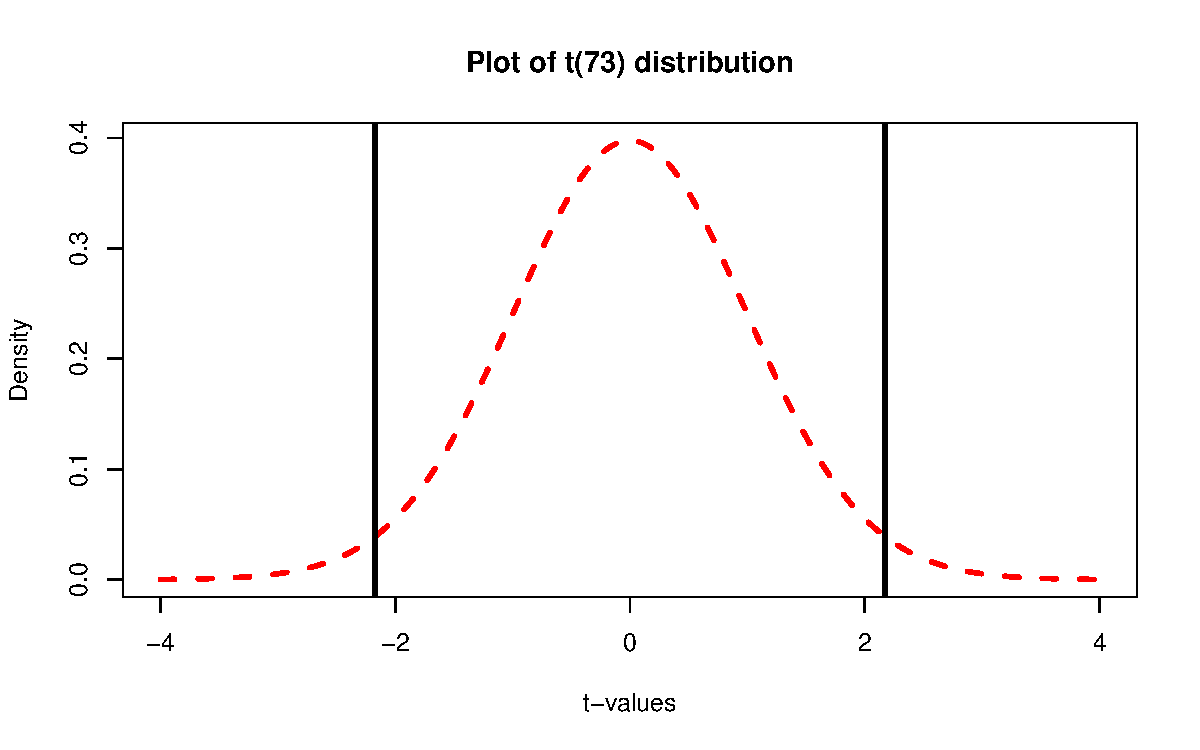
\includegraphics{02-reintroductionToStatistics_files/figure-latex/Figure2-20-1.pdf}
\caption{\label{fig:Figure2-20}Plot of \(t(73)\) with cut-offs for putting 95\% of
distributions in the middle.}
\end{figure}

For 95\% confidence intervals, the multiplier is going to be close to 2
and anything else is a sign of a mistake. We can use R to get the
multipliers for confidence intervals using the \texttt{qt} function in a
similar fashion to how \texttt{qdata} was used in the bootstrap results,
except that this new value must be used in the previous confidence
interval formula. This function produces values for requested
percentiles, so if we want to put 95\% in the middle, we place 2.5\% in
each tail of the distribution and need to request the 97.5th percentile.
Because the \(t\)-distribution is always symmetric around 0, we merely
need to look up the value for the 97.5th percentile and know that the
multiplier for the 2.5th percentile is just \(-t^*\). The \(t^*\)
multiplier to form the confidence interval is 1.993 for a 95\%
confidence interval when the \(df=73\) based on the results from
\texttt{qt}:

\begin{Shaded}
\begin{Highlighting}[]
\KeywordTok{qt}\NormalTok{(}\FloatTok{0.975}\NormalTok{, }\DataTypeTok{df=}\DecValTok{73}\NormalTok{)}
\end{Highlighting}
\end{Shaded}

\begin{verbatim}
## [1] 1.992997
\end{verbatim}

Note that the 2.5th percentile is just the negative of this value due to
symmetry and the real source of the minus in the minus/plus in the
formula for the confidence interval.

\begin{Shaded}
\begin{Highlighting}[]
\KeywordTok{qt}\NormalTok{(}\FloatTok{0.025}\NormalTok{, }\DataTypeTok{df=}\DecValTok{73}\NormalTok{)}
\end{Highlighting}
\end{Shaded}

\begin{verbatim}
## [1] -1.992997
\end{verbatim}

We can also re-write the confidence interval formula into a slightly
more general form as

\[\bar{x}_1 - \bar{x}_2 \mp t^*_{df}SE_{\bar{x}_1 - \bar{x}_2}\ \text{ OR }\ 
\bar{x}_1 - \bar{x}_2 \mp ME\]

where
\(SE_{\bar{x}_1 - \bar{x}_2} = s_p\sqrt{\frac{1}{n_1}+\frac{1}{n_2}}\)
and \(ME = t^*_{df}SE_{\bar{x}_1 - \bar{x}_2}\). In some situations,
researchers will report the \textbf{\emph{standard error}} (SE) or
\textbf{\emph{margin of error}} (ME) as a method of quantifying the
uncertainty in a statistic. The SE is an estimate of the standard
deviation of the statistic (here \(\bar{x}_1 - \bar{x}_2\)) and the ME
is an estimate of the precision of a statistic that can be used to
directly form a confidence interval. The ME depends on the choice of
confidence level although 95\% is almost always selected.

To finish this example, R can be used to help you do calculations much
like a calculator except with much more power ``under the hood''. You
have to make sure you are careful with using \texttt{(\ )} to group
items and remember that the asterisk (*) is used for multiplication in
R. We need the pertinent information which is available from the
\texttt{favstats} output repeated below to calculate the confidence
interval ``by hand'' using R.

\begin{Shaded}
\begin{Highlighting}[]
\KeywordTok{favstats}\NormalTok{(Years}\OperatorTok{~}\NormalTok{Attr, }\DataTypeTok{data=}\NormalTok{MockJury2)}
\end{Highlighting}
\end{Shaded}

\begin{verbatim}
##           Attr min Q1 median Q3 max     mean       sd  n missing
## 1      Average   1  2      3  5  12 3.973684 2.823519 38       0
## 2 Unattractive   1  2      5 10  15 5.810811 4.364235 37       0
\end{verbatim}

Start with typing the following command to calculate \(s_p\) and store
it in a variable named \texttt{sp}:

\begin{Shaded}
\begin{Highlighting}[]
\NormalTok{sp <-}\StringTok{ }\KeywordTok{sqrt}\NormalTok{(((}\DecValTok{38}\OperatorTok{-}\DecValTok{1}\NormalTok{)}\OperatorTok{*}\NormalTok{(}\FloatTok{2.8235}\OperatorTok{^}\DecValTok{2}\NormalTok{)}\OperatorTok{+}\NormalTok{(}\DecValTok{37}\OperatorTok{-}\DecValTok{1}\NormalTok{)}\OperatorTok{*}\NormalTok{(}\FloatTok{4.364}\OperatorTok{^}\DecValTok{2}\NormalTok{))}\OperatorTok{/}\NormalTok{(}\DecValTok{38}\OperatorTok{+}\DecValTok{37}\OperatorTok{-}\DecValTok{2}\NormalTok{))}
\NormalTok{sp}
\end{Highlighting}
\end{Shaded}

\begin{verbatim}
## [1] 3.665036
\end{verbatim}

Then calculate the confidence interval that \texttt{t.test} provided
using:

\begin{Shaded}
\begin{Highlighting}[]
\FloatTok{3.974}\OperatorTok{-}\FloatTok{5.811}\OperatorTok{+}\KeywordTok{c}\NormalTok{(}\OperatorTok{-}\DecValTok{1}\NormalTok{,}\DecValTok{1}\NormalTok{)}\OperatorTok{*}\KeywordTok{qt}\NormalTok{(.}\DecValTok{975}\NormalTok{,}\DataTypeTok{df=}\DecValTok{73}\NormalTok{)}\OperatorTok{*}\NormalTok{sp}\OperatorTok{*}\KeywordTok{sqrt}\NormalTok{(}\DecValTok{1}\OperatorTok{/}\DecValTok{38}\OperatorTok{+}\DecValTok{1}\OperatorTok{/}\DecValTok{37}\NormalTok{)}
\end{Highlighting}
\end{Shaded}

\begin{verbatim}
## [1] -3.5240302 -0.1499698
\end{verbatim}

The previous code uses \texttt{c(-1,\ 1)} times the margin of error to
subtract and add the ME to the difference in the sample means
(\(3.974-5.811\)), which generates the lower and then upper bounds of
the confidence interval. If desired, we can also use just the last
portion of the previous calculation to find the margin of error, which
is 1.69 here.

\begin{Shaded}
\begin{Highlighting}[]
\KeywordTok{qt}\NormalTok{(.}\DecValTok{975}\NormalTok{,}\DataTypeTok{df=}\DecValTok{73}\NormalTok{)}\OperatorTok{*}\NormalTok{sp}\OperatorTok{*}\KeywordTok{sqrt}\NormalTok{(}\DecValTok{1}\OperatorTok{/}\DecValTok{38}\OperatorTok{+}\DecValTok{1}\OperatorTok{/}\DecValTok{37}\NormalTok{)}
\end{Highlighting}
\end{Shaded}

\begin{verbatim}
## [1] 1.68703
\end{verbatim}

\section{Bootstrap confidence intervals for difference in
GPAs}\label{section2-9}

We can now apply the new confidence interval methods on the STAT 217
grade data. This time we start with the parametric 95\% confidence
interval ``by hand'' in R and then use \texttt{t.test} to verify our
result. The \texttt{favstats} output provides us with the required
information to calculate the confidence interval:

\begin{Shaded}
\begin{Highlighting}[]
\KeywordTok{favstats}\NormalTok{(GPA}\OperatorTok{~}\NormalTok{Sex,}\DataTypeTok{data=}\NormalTok{s217)}
\end{Highlighting}
\end{Shaded}

\begin{verbatim}
##   Sex  min  Q1 median   Q3 max     mean        sd  n missing
## 1   F 2.50 3.1  3.400 3.70   4 3.338378 0.4074549 37       0
## 2   M 1.96 2.8  3.175 3.46   4 3.088571 0.4151789 42       0
\end{verbatim}

The \(df\) are \(37+42-2 = 77\). Using the SDs from the two groups and
their sample sizes, we can calculate \(s_p\):

\begin{Shaded}
\begin{Highlighting}[]
\NormalTok{sp <-}\StringTok{ }\KeywordTok{sqrt}\NormalTok{(((}\DecValTok{37}\OperatorTok{-}\DecValTok{1}\NormalTok{)}\OperatorTok{*}\NormalTok{(}\FloatTok{0.4075}\OperatorTok{^}\DecValTok{2}\NormalTok{)}\OperatorTok{+}\NormalTok{(}\DecValTok{42}\OperatorTok{-}\DecValTok{1}\NormalTok{)}\OperatorTok{*}\NormalTok{(}\FloatTok{0.41518}\OperatorTok{^}\DecValTok{2}\NormalTok{))}\OperatorTok{/}\NormalTok{(}\DecValTok{37}\OperatorTok{+}\DecValTok{42}\OperatorTok{-}\DecValTok{2}\NormalTok{))}
\NormalTok{sp}
\end{Highlighting}
\end{Shaded}

\begin{verbatim}
## [1] 0.4116072
\end{verbatim}

The margin of error is:

\begin{Shaded}
\begin{Highlighting}[]
\KeywordTok{qt}\NormalTok{(.}\DecValTok{975}\NormalTok{,}\DataTypeTok{df=}\DecValTok{77}\NormalTok{)}\OperatorTok{*}\NormalTok{sp}\OperatorTok{*}\KeywordTok{sqrt}\NormalTok{(}\DecValTok{1}\OperatorTok{/}\DecValTok{37}\OperatorTok{+}\DecValTok{1}\OperatorTok{/}\DecValTok{42}\NormalTok{)}
\end{Highlighting}
\end{Shaded}

\begin{verbatim}
## [1] 0.1847982
\end{verbatim}

All together, the 95\% confidence interval is:

\begin{Shaded}
\begin{Highlighting}[]
\FloatTok{3.338}\OperatorTok{-}\FloatTok{3.0886}\OperatorTok{+}\KeywordTok{c}\NormalTok{(}\OperatorTok{-}\DecValTok{1}\NormalTok{,}\DecValTok{1}\NormalTok{)}\OperatorTok{*}\KeywordTok{qt}\NormalTok{(.}\DecValTok{975}\NormalTok{,}\DataTypeTok{df=}\DecValTok{77}\NormalTok{)}\OperatorTok{*}\NormalTok{sp}\OperatorTok{*}\KeywordTok{sqrt}\NormalTok{(}\DecValTok{1}\OperatorTok{/}\DecValTok{37}\OperatorTok{+}\DecValTok{1}\OperatorTok{/}\DecValTok{42}\NormalTok{)}
\end{Highlighting}
\end{Shaded}

\begin{verbatim}
## [1] 0.0646018 0.4341982
\end{verbatim}

So we are 95\% confident that the difference in the true mean GPAs
between females and males (females minus males) is between 0. 065 and 0.
434 GPA points. We get a similar\footnote{We rounded the means a little
  and that caused the small difference in results.} result from the
\texttt{t.test} output:

\begin{Shaded}
\begin{Highlighting}[]
\KeywordTok{t.test}\NormalTok{(GPA}\OperatorTok{~}\NormalTok{Sex,}\DataTypeTok{data=}\NormalTok{s217,}\DataTypeTok{var.equal=}\NormalTok{T)}
\end{Highlighting}
\end{Shaded}

\begin{verbatim}
## 
##  Two Sample t-test
## 
## data:  GPA by Sex
## t = 2.6919, df = 77, p-value = 0.008713
## alternative hypothesis: true difference in means is not equal to 0
## 95 percent confidence interval:
##  0.06501838 0.43459552
## sample estimates:
## mean in group F mean in group M 
##        3.338378        3.088571
\end{verbatim}

Note that we can easily switch to 90\% or 99\% confidence intervals by
simply changing the percentile in \texttt{qt} or changing
\texttt{conf.\ level} in the \texttt{t.test} function. In the following
two lines of code, we added octothorpes\footnote{You can correctly call
  octothorpes \emph{number} symbols or, in the twitter verse,
  \emph{hashtags}. For more on this symbol, see
  ``\url{http://blog.dictionary.com/octothorpe/}''. I usually call them
  number symbols too.}(\#) and then some text after function calls to
explain what is being calculated. In computer code, octothorpes provide
a way of adding comments that tell the software (here R) to ignore any
text after a ``\#'' on a given line. In the color version of the text,
comments are also clearly distinguished.

\begin{Shaded}
\begin{Highlighting}[]
\KeywordTok{qt}\NormalTok{(.}\DecValTok{95}\NormalTok{,}\DataTypeTok{df=}\DecValTok{77}\NormalTok{) }\CommentTok{# For 90% confidence and 77 df}
\end{Highlighting}
\end{Shaded}

\begin{verbatim}
## [1] 1.664885
\end{verbatim}

\begin{Shaded}
\begin{Highlighting}[]
\KeywordTok{qt}\NormalTok{(.}\DecValTok{995}\NormalTok{,}\DataTypeTok{df=}\DecValTok{77}\NormalTok{) }\CommentTok{#For 99% confidence and 77 df}
\end{Highlighting}
\end{Shaded}

\begin{verbatim}
## [1] 2.641198
\end{verbatim}

\begin{Shaded}
\begin{Highlighting}[]
\KeywordTok{t.test}\NormalTok{(GPA}\OperatorTok{~}\NormalTok{Sex,}\DataTypeTok{data=}\NormalTok{s217,}\DataTypeTok{var.equal=}\NormalTok{T,}\DataTypeTok{conf.level=}\FloatTok{0.90}\NormalTok{)}
\end{Highlighting}
\end{Shaded}

\begin{verbatim}
## 
##  Two Sample t-test
## 
## data:  GPA by Sex
## t = 2.6919, df = 77, p-value = 0.008713
## alternative hypothesis: true difference in means is not equal to 0
## 90 percent confidence interval:
##  0.09530553 0.40430837
## sample estimates:
## mean in group F mean in group M 
##        3.338378        3.088571
\end{verbatim}

\begin{Shaded}
\begin{Highlighting}[]
\KeywordTok{t.test}\NormalTok{(GPA}\OperatorTok{~}\NormalTok{Sex,}\DataTypeTok{data=}\NormalTok{s217,}\DataTypeTok{var.equal=}\NormalTok{T,}\DataTypeTok{conf.level=}\FloatTok{0.99}\NormalTok{)}
\end{Highlighting}
\end{Shaded}

\begin{verbatim}
## 
##  Two Sample t-test
## 
## data:  GPA by Sex
## t = 2.6919, df = 77, p-value = 0.008713
## alternative hypothesis: true difference in means is not equal to 0
## 99 percent confidence interval:
##  0.004703598 0.494910301
## sample estimates:
## mean in group F mean in group M 
##        3.338378        3.088571
\end{verbatim}

As a review of some basic ideas with confidence intervals make sure you
can answer the following questions:

\begin{enumerate}
\def\labelenumi{\arabic{enumi}.}
\item
  What is the impact of increasing the confidence level in this
  situation?
\item
  What happens to the width of the confidence interval if the size of
  the SE increases or decreases?
\item
  What about increasing the sample size -- should that increase or
  decrease the width of the interval?
\end{enumerate}

All the general results you learned before about impacts to widths of
CIs hold in this situation whether we are considering the parametric or
bootstrap methods\ldots{}

To finish this example, we will generate the comparable bootstrap 90\%
confidence interval using the bootstrap distribution in Figure
\ref{fig:Figure2-21}.

\begin{Shaded}
\begin{Highlighting}[]
\NormalTok{Tobs <-}\StringTok{ }\KeywordTok{diffmean}\NormalTok{(GPA }\OperatorTok{~}\StringTok{ }\NormalTok{Sex, }\DataTypeTok{data=}\NormalTok{s217); Tobs}
\end{Highlighting}
\end{Shaded}

\begin{verbatim}
##   diffmean 
## -0.2498069
\end{verbatim}

\begin{Shaded}
\begin{Highlighting}[]
\KeywordTok{par}\NormalTok{(}\DataTypeTok{mfrow=}\KeywordTok{c}\NormalTok{(}\DecValTok{1}\NormalTok{,}\DecValTok{2}\NormalTok{))}
\NormalTok{B<-}\StringTok{ }\DecValTok{1000}
\NormalTok{Tstar<-}\KeywordTok{matrix}\NormalTok{(}\OtherTok{NA}\NormalTok{,}\DataTypeTok{nrow=}\NormalTok{B)}
\ControlFlowTok{for}\NormalTok{ (b }\ControlFlowTok{in}\NormalTok{ (}\DecValTok{1}\OperatorTok{:}\NormalTok{B))\{}
\NormalTok{  Tstar[b]<-}\KeywordTok{diffmean}\NormalTok{(GPA }\OperatorTok{~}\StringTok{ }\NormalTok{Sex, }\DataTypeTok{data=}\KeywordTok{resample}\NormalTok{(s217))}
\NormalTok{  \}}
\KeywordTok{qdata}\NormalTok{(Tstar,.}\DecValTok{05}\NormalTok{)}
\end{Highlighting}
\end{Shaded}

\begin{verbatim}
##          p   quantile 
##  0.0500000 -0.4032273
\end{verbatim}

\begin{Shaded}
\begin{Highlighting}[]
\KeywordTok{qdata}\NormalTok{(Tstar,.}\DecValTok{95}\NormalTok{)}
\end{Highlighting}
\end{Shaded}

\begin{verbatim}
##           p    quantile 
##  0.95000000 -0.09521925
\end{verbatim}

\begin{Shaded}
\begin{Highlighting}[]
\NormalTok{quantiles<-}\KeywordTok{qdata}\NormalTok{(Tstar,}\KeywordTok{c}\NormalTok{(.}\DecValTok{05}\NormalTok{,.}\DecValTok{95}\NormalTok{))}
\NormalTok{quantiles}
\end{Highlighting}
\end{Shaded}

\begin{verbatim}
##        quantile    p
## 5%  -0.40322729 0.05
## 95% -0.09521925 0.95
\end{verbatim}

The output tells us that the 90\% confidence interval is from -0.393 to
-0.094 GPA points. The bootstrap distribution with the observed
difference in the sample means and these cut-offs is displayed in Figure
\ref{fig:Figure2-21} using this code:






\begin{figure}
\centering
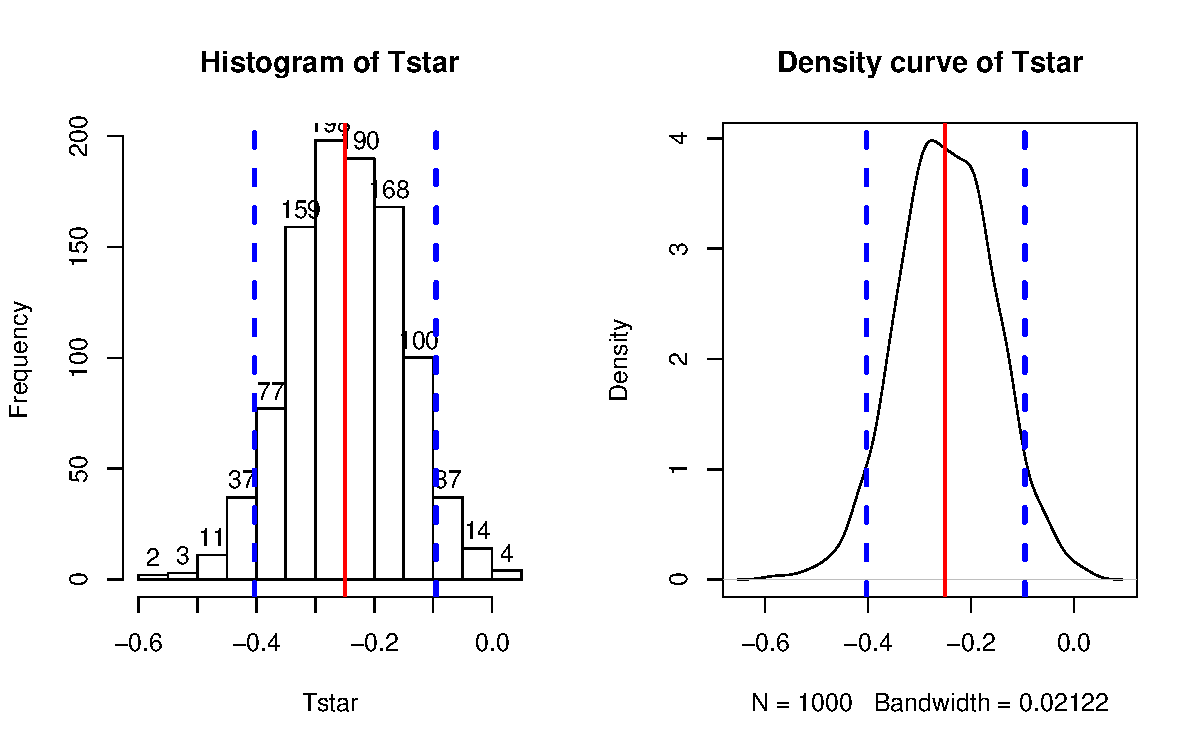
\includegraphics{02-reintroductionToStatistics_files/figure-latex/Figure2-21-1.pdf}
\caption{\label{fig:Figure2-21}Histogram and density curve of bootstrap distribution of
difference in sample mean GPAs (male minus female) with observed
difference (solid vertical line) and quantiles that delineate the 90\%
confidence intervals (dashed vertical lines).}
\end{figure}

\begin{Shaded}
\begin{Highlighting}[]
\KeywordTok{par}\NormalTok{(}\DataTypeTok{mfrow=}\KeywordTok{c}\NormalTok{(}\DecValTok{1}\NormalTok{,}\DecValTok{2}\NormalTok{))}
\KeywordTok{hist}\NormalTok{(Tstar,}\DataTypeTok{labels=}\NormalTok{T)}
\KeywordTok{abline}\NormalTok{(}\DataTypeTok{v=}\NormalTok{Tobs,}\DataTypeTok{col=}\StringTok{"red"}\NormalTok{,}\DataTypeTok{lwd=}\DecValTok{2}\NormalTok{)}
\KeywordTok{abline}\NormalTok{(}\DataTypeTok{v=}\NormalTok{quantiles}\OperatorTok{$}\NormalTok{quantile,}\DataTypeTok{col=}\StringTok{"blue"}\NormalTok{,}\DataTypeTok{lwd=}\DecValTok{3}\NormalTok{,}\DataTypeTok{lty=}\DecValTok{2}\NormalTok{)}
\KeywordTok{plot}\NormalTok{(}\KeywordTok{density}\NormalTok{(Tstar),}\DataTypeTok{main=}\StringTok{"Density curve of Tstar"}\NormalTok{)}
\KeywordTok{abline}\NormalTok{(}\DataTypeTok{v=}\NormalTok{Tobs,}\DataTypeTok{col=}\StringTok{"red"}\NormalTok{,}\DataTypeTok{lwd=}\DecValTok{2}\NormalTok{)}
\KeywordTok{abline}\NormalTok{(}\DataTypeTok{v=}\NormalTok{quantiles}\OperatorTok{$}\NormalTok{quantile,}\DataTypeTok{col=}\StringTok{"blue"}\NormalTok{,}\DataTypeTok{lwd=}\DecValTok{3}\NormalTok{,}\DataTypeTok{lty=}\DecValTok{2}\NormalTok{)}
\end{Highlighting}
\end{Shaded}

In the previous output, the parametric 90\% confidence interval is from
0.095 to 0.404, suggesting similar results again from the two approaches
once you account for the two different orders of differencing of the
groups. Based on the bootstrap CI, we can say that we are 90\% confident
that the difference in the true mean GPAs for STAT 217 students is
between -0.393 to -0.094 GPA points (male minus females). Because sex
cannot be assigned to the subjects, we cannot infer that sex is causing
this difference and because this was a voluntary response sample of STAT
217 students in a given semester, we cannot infer that a difference of
this size would apply to all STAT 217 students or even students in
another semester.

Throughout the semester, pay attention to the distinctions between
parameters and statistics, focusing on the differences between estimates
based on the sample and inferences for the population of interest in the
form of the parameters of interest. Remember that statistics are
summaries of the sample information and parameters are characteristics
of populations (which we rarely know). And that our inferences are
limited to the population that we randomly sampled from, if we randomly
sampled.

\section{Chapter summary}\label{section2-10}

In this chapter, we reviewed basic statistical inference methods in the
context of a two-sample mean problem. You were introduced to using R to
do permutation testing and generate bootstrap confidence intervals as
well as obtaining parametric \(t\)-test and confidence intervals in this
same situation. You should have learned how to use a \texttt{for} loop
for doing the nonparametric inferences and the \texttt{t.test} function
for generating parametric inferences. In the two examples considered,
the parametric and nonparametric methods provided similar results,
suggesting that the assumptions were at least close to being met for the
parametric procedures. When parametric and nonparametric approaches
disagree, the nonparametric methods are likely to be more trustworthy
since they have less restrictive assumptions but can still have
problems.

When the noted conditions are not met in a hypothesis testing situation,
the Type I error rates can be inflated, meaning that we reject the null
hypothesis more often than we have allowed to occur by chance.
Specifically, we could have a situation where our assumed 5\%
significance level test might actually reject the null when it is true
20\% of the time. If this is occurring, we call a procedure
\textbf{\emph{liberal}} (it rejects too easily) and if the procedure is
liberal, how could we trust a small p-value to be a ``real'' result and
not just an artifact of violating the assumptions of the procedure?
Likewise, for confidence intervals we hope that our 95\% confidence
level procedure, when repeated, will contain the true parameter 95\% of
the time. If our assumptions are violated, we might actually have an
80\% confidence level procedure and it makes it hard to trust the
reported results for our observed data set. Statistical inference relies
on a belief in the methods underlying our inferences. If we don't trust
our assumptions, we shouldn't trust the conclusions to perform the way
we want them to. As sample sizes increase and/or violations of
conditions lessen, then the procedures will perform better. In Chapter
\ref{chapter3}, we'll learn some new tools for doing diagnostics to help
us assess how much those conditions are violated.

\section{Summary of important R code}\label{section2-11}

The main components of R code used in this chapter follow with
components to modify in red, remembering that any R packages mentioned
need to be installed and loaded for this code to have a chance of
working:

\begin{itemize}
\item
  summary(\textcolor{red}{DATASETNAME})

  \begin{itemize}
  \tightlist
  \item
    Provides numerical summaries of all variables in the data set.
  \end{itemize}
\item
  t.test(\textcolor{red}{Y} \textasciitilde{} \textcolor{red}{X},
  data=\textcolor{red}{DATASETNAME}, conf.level=0.95)

  \begin{itemize}
  \tightlist
  \item
    Provides two-sample t-test test statistic, df, p-value, and 95\%
    confidence interval.
  \end{itemize}
\item
  2*pt(abs(\textcolor{red}{Tobs}), df=\textcolor{red}{DF}, lower.tail=F)

  \begin{itemize}
  \tightlist
  \item
    Finds the two-sided test p-value for an observed 2-sample t-test
    statistic of \texttt{Tobs}.
  \end{itemize}
\item
  hist(\textcolor{red}{DATASETNAME\$Y})

  \begin{itemize}
  \tightlist
  \item
    Makes a histogram of a variable named \texttt{Y} from the data set
    of interest.
  \end{itemize}
\item
  boxplot(\textcolor{red}{Y}\textasciitilde{}\textcolor{red}{X},
  data=\textcolor{red}{DATASETNAME})

  \begin{itemize}
  \tightlist
  \item
    Makes a boxplot of a variable named Y for groups in X from the data
    set.
  \end{itemize}
\item
  beanplot(\textcolor{red}{Y}\textasciitilde{}\textcolor{red}{X},
  data=\textcolor{red}{DATASETNAME})

  \begin{itemize}
  \item
    Requires the \texttt{beanplot} package is loaded.
  \item
    Makes a beanplot of a variable named Y for groups in X from the data
    set.
  \end{itemize}
\item
  mean(\textcolor{red}{Y}\textasciitilde{}\textcolor{red}{X},
  data=\textcolor{red}{DATASETNAME});
  sd(\textcolor{red}{Y}\textasciitilde{}\textcolor{red}{X},
  data=\textcolor{red}{DATASETNAME})

  \begin{itemize}
  \item
    This usage of \texttt{mean} and \texttt{sd} requires the
    \texttt{mosaic} package.
  \item
    Provides the mean and sd of responses of Y for each group described
    in X.
  \end{itemize}
\item
  favstats(\textcolor{red}{Y}\textasciitilde{}\textcolor{red}{X},
  data=\textcolor{red}{DATASETNAME})

  \begin{itemize}
  \tightlist
  \item
    Provides numerical summaries of Y by groups described in X.
  \end{itemize}
\item
  Tobs \texttt{\textless{}-}
  t.test(\textcolor{red}{Y}\textasciitilde{}\textcolor{red}{X},
  data=\textcolor{red}{DATASETNAME}, var.equal=T)\$statistic; Tobs\\
  B \texttt{\textless{}-} 1000\\
  Tstar \texttt{\textless{}-} matrix(NA, nrow=B)\\
  for (b in (1:B))\{\\
  Tstar{[}b{]} \texttt{\textless{}-}
  t.test(\textcolor{red}{Y}\textasciitilde{}shuffle(\textcolor{red}{X}),
  data=\textcolor{red}{DATASETNAME}, var.equal=T)\$statistic\\
  \}

  \begin{itemize}
  \tightlist
  \item
    Code to run a \texttt{for} loop to generate 1000 permuted versions
    of the test statistic using the \texttt{shuffle} function and keep
    track of the results in \texttt{Tstar}
  \end{itemize}
\item
  pdata(Tstar, abs(\textcolor{red}{Tobs}, lower.tail=F)

  \begin{itemize}
  \tightlist
  \item
    Finds the proportion of the permuted test statistics in Tstar that
    are less than -\textbar{}Tobs\textbar{} or greater than
    \textbar{}Tobs\textbar{}, useful for finding the two-sided test
    p-value.
  \end{itemize}
\item
  Tobs \texttt{\textless{}-}
  diffmean(\textcolor{red}{Y}\textasciitilde{}\textcolor{red}{X},
  data=\textcolor{red}{DATASETNAME}, var.equal=T)\$statistic; Tobs\\
  B \texttt{\textless{}-} 1000\\
  Tstar \texttt{\textless{}-} matrix(NA, nrow=B)\\
  for (b in (1:B))\{\\
  Tstar{[}b{]} \texttt{\textless{}-}
  diffmean(\textcolor{red}{Y}\textasciitilde{}\textcolor{red}{X},
  data=resample(\textcolor{red}{DATASETNAME}))\\
  \}

  \begin{itemize}
  \tightlist
  \item
    Code to run a \texttt{for} loop to generate 1000 bootstrapped
    versions of the data set using the \texttt{resample} function and
    keep track of the results of the statistic in \texttt{Tstar}.
  \end{itemize}
\item
  qdata(Tstar, c(0. 025, 0. 975))

  \begin{itemize}
  \tightlist
  \item
    Provides the values that delineate the middle 95\% of the results in
    the bootstrap distribution (\texttt{Tstar})
  \end{itemize}
\end{itemize}

\section{Practice problems}\label{section2-12}

Load the \texttt{HELPrct} data set from the \texttt{mosaicData} package
\citep{R-mosaicData} (you need to install the \texttt{mosaicData}
package once to be able to load it). The HELP study was a clinical trial
for adult inpatients recruited from a detoxification unit. Patients with
no primary care physician were randomly assigned to receive a
multidisciplinary assessment and a brief motivational intervention or
usual care and various outcomes were observed. Two of the variables in
the data set are \texttt{sex}, a factor with levels male and female and
\texttt{daysanysub} which is the time (in days) to first use of any
substance post-detox. We are interested in the difference in mean number
of days to first use of any substance post-detox between males and
females. There are some missing responses and the following code will
produce \texttt{favstats} with the missing values and then provide a
data set that for complete observations by applying the \texttt{na.omit}
function that removes any observations with missing values.

\begin{verbatim}
require(mosaicData)
data(HELPrct)
HELPrct <- HELPrct[, c("daysanysub", "sex")] #Just focus on two variables
HELPrct <- na.omit(HELPrct2) #Removes subjects with missing
favstats(daysanysub~sex, data=HELPrct2)
favstats(daysanysub~sex, data=HELPrct3)
\end{verbatim}

2.1. Based on the results provided, how many observations were missing
for males and females? Missing values here likely mean that the subjects
didn't use any substances post-detox in the time of the study but might
have at a later date -- the study just didn't run long enough. This is
called \textbf{\emph{censoring}}. What is the problem with the numerical
summaries here if the missing responses were all something larger than
the largest observation?

2.2. Make a beanplot and a boxplot of \texttt{daysanysub}
\textasciitilde{} \texttt{sex} using the \texttt{HELPrct3} data set
created above. Compare the distributions, recommending parametric or
nonparametric inferences.

2.3. Generate the permutation results and write out the 6+ steps of the
hypothesis test, making sure to note the numerical value of observed
test statistic you are using and include a discussion of the scope of
inference.

2.4. Interpret the p-value for these results.

2.5. Generate the parametric \texttt{t.test} results, reporting the
test-statistic, its distribution under the null hypothesis, and compare
the p-value to those observed using the permutation approach.

2.6. Make and interpret a 95\% bootstrap confidence interval for the
difference in the means.

\chapter{One-Way ANOVA}\label{chapter3}

\section{Situation}\label{section3-1}

In Chapter \ref{chapter2}, tools for comparing the means of two groups
were considered. More generally, these methods are used for a
quantitative response and a categorical explanatory variable (group)
which had two and only two levels. The full prisoner rating data set
actually contained three groups (Figure \ref{fig:Figure3-1} with
\emph{Beautiful}, \emph{Average}, and \emph{Unattractive} rated pictures
randomly assigned to the subjects for sentence ratings. In a situation
with more than two groups, we have two choices. First, we could rely on
our two group comparisons, performing tests for every possible pair
(\emph{Beautiful} vs \emph{Average}, \emph{Beautiful} vs
\emph{Unattractive}, and \emph{Average} vs \emph{Unattractive}). We
spent Chapter \ref{chapter2} doing inferences for differences between
\emph{Average} and \emph{Unattractive}. The other two comparisons would
lead us to initially end up with three p-values and no direct answer
about our initial question of interest -- is there some overall
difference in the average sentences provided across the groups? In this
chapter, we will learn a new method, called \textbf{\emph{Analysis of
Variance}}, or \textbf{\emph{One-Way ANOVA}} since there is just
one\footnote{In Chapter \ref{chapter4}, methods are discussed for when
  there are two categorical explanatory variables that is called the
  Two-Way ANOVA and related ANOVA tests are used in Chapter
  \ref{chapter8} for working with extensions of these models.} grouping
variable. After we perform our One-Way ANOVA test for overall evidence
of a difference, we will revisit the comparisons similar to those
considered in Chapter \ref{chapter2} to get more details on specific
differences among \emph{all} the pairs of groups -- what we call
\textbf{\emph{pair-wise comparisons}}. An issue is created when you
perform many tests simultaneously and we will augment our previous
methods with an adjusted method for pairwise comparisons to make our
results valid called \textbf{\emph{Tukey's Honest Significant
Difference}}.

To make this more concrete, we return to the original MockJury data,
making side-by-side boxplots and beanplots (Figure \ref{fig:Figure3-1}
as well summarizing the sentences for the three groups using
\texttt{favstats}.




\begin{Shaded}
\begin{Highlighting}[]
\KeywordTok{require}\NormalTok{(heplots)}
\KeywordTok{require}\NormalTok{(mosaic)}
\KeywordTok{data}\NormalTok{(MockJury)}
\KeywordTok{par}\NormalTok{(}\DataTypeTok{mfrow=}\KeywordTok{c}\NormalTok{(}\DecValTok{1}\NormalTok{,}\DecValTok{2}\NormalTok{))}
\KeywordTok{boxplot}\NormalTok{(Years}\OperatorTok{~}\NormalTok{Attr,}\DataTypeTok{data=}\NormalTok{MockJury)}
\KeywordTok{require}\NormalTok{(beanplot)}
\KeywordTok{beanplot}\NormalTok{(Years}\OperatorTok{~}\NormalTok{Attr,}\DataTypeTok{data=}\NormalTok{MockJury,}\DataTypeTok{log=}\StringTok{""}\NormalTok{,}\DataTypeTok{col=}\StringTok{"bisque"}\NormalTok{,}\DataTypeTok{method=}\StringTok{"jitter"}\NormalTok{)}
\end{Highlighting}
\end{Shaded}

\begin{figure}
\centering
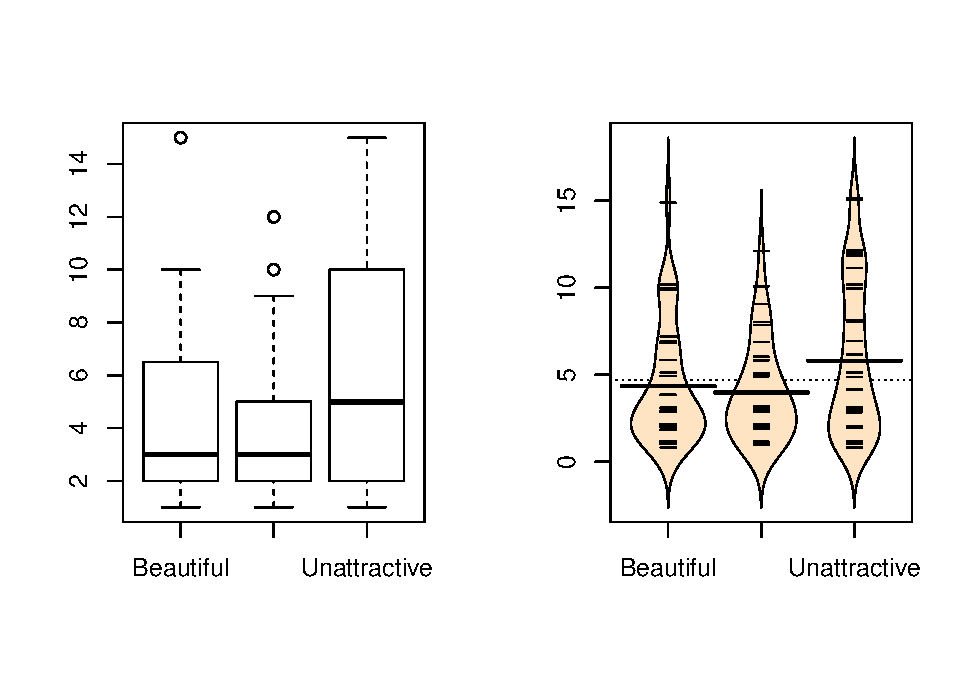
\includegraphics{03-oneWayAnova_files/figure-latex/Figure3-1-1.pdf}
\caption{\label{fig:Figure3-1}Boxplot and beanplot of the sentences (years) for the three
treatment groups.}
\end{figure}

\begin{Shaded}
\begin{Highlighting}[]
\KeywordTok{favstats}\NormalTok{(Years}\OperatorTok{~}\NormalTok{Attr,}\DataTypeTok{data=}\NormalTok{MockJury)}
\end{Highlighting}
\end{Shaded}

\begin{verbatim}
##           Attr min Q1 median   Q3 max     mean       sd  n missing
## 1    Beautiful   1  2      3  6.5  15 4.333333 3.405362 39       0
## 2      Average   1  2      3  5.0  12 3.973684 2.823519 38       0
## 3 Unattractive   1  2      5 10.0  15 5.810811 4.364235 37       0
\end{verbatim}

There are slight differences in the sample sizes in the three groups
with 37 \emph{Unattractive}, 38 \emph{Average} and 39 \emph{Beautiful}
group responses, providing a data set has a total sample size of
\(N=114\). The \emph{Beautiful} and \emph{Average} groups do not appear
to be very different with means of 4.33 and 3.97 years. In Chapter
\ref{chapter2}, we found moderate evidence regarding the difference in
\emph{Average}and \emph{Unattractive}. It is less clear whether we might
find evidence of a difference between \emph{Beautiful} and
\emph{Unattractive} groups since we are comparing means of 5.81 and 4.33
years. All the distributions appear to be right skewed with relatively
similar shapes. The variability in \emph{Average} and
\emph{Unattractive} groups seems like it could be slightly different
leading to an overall concern of whether the variability is the same in
all the groups.

\section{Linear model for One-Way ANOVA (cell-means and
reference-coding)}\label{section3-2}

We introduced the statistical model \(y_{ij} = \mu_j+\varepsilon_j\) in
Chapter \ref{chapter2} for the situation with \(j = 1 \text{ or } 2\) to
denote a situation where there were two groups and, for the model that
is consistent with the alternative hypothesis, the means differed. Now
we have three groups and the previous model can be extended to this new
situation by allowing \(j\) to be 1, 2, or 3. Now that we have more than
two groups, we need to admit that what we were doing in Chapter
\ref{chapter2} was actually fitting what is called a
\textbf{\emph{linear model}}. The linear model assumes that the
responses follow a normal distribution with the linear model defining
the mean, all observations have the same variance, and the parameters
for the mean in the model enter linearly. This last condition is hard to
explain at this level of material -- it is sufficient to know that there
models where the parameters enter the model nonlinearly and that they
are beyond the scope of this course. The result of this constraint is
that we will be able to use the same general modeling framework for the
methods introduced in Chapters \ref{chapter3}, \ref{chapter4},
\ref{chapter6}, \ref{chapter7}, and \ref{chapter8}.

As in Chapter \ref{chapter2}, we have a null hypothesis that defines a
situation (and model) where all the groups have the same mean.
Specifically, the \textbf{\emph{null hypothesis}} in the general
situation with \(J\) groups (\(J\ge 2\)) is to have all the
\textbf{true} group means equal,

\[H_0:\mu_1 = \ldots \mu_J.\]

This defines a model where all the groups have the same mean so it can
be defined in terms of a single mean, \(\mu\), for the \(i^{th}\)
observation from the \(j^{th}\) group as
\(y_{ij} = \mu+\varepsilon_{ij}\). This is not the model that most
researchers want to be the final description of their study as it
implies no difference in the groups. There is more caution required to
specify the alternative hypothesis with more than two groups. The
\textbf{\emph{alternative hypothesis}} needs to be the logical negation
of this null hypothesis of all groups having equal means; to make the
null hypothesis false, we only need one group to differ but more than
one group could differ from the others. Essentially, there are many ways
to ``violate'' the null hypothesis so we choose some delicate wording
for the alternative hypothesis when there are more than 2 groups.
Specifically, we state the alternative as

\[H_A: \text{ Not all } \mu_j \text{ are equal}\]

or, in words, \textbf{at least one of the true means differs among the J
groups}. You will be attracted to trying to say that all means are
different in the alternative but we do not put this strict a requirement
in place to reject the null hypothesis. The alternative model allows all
the true group means to differ but does require that they differ with

\[{\color{red}{\mu_j}}+\varepsilon_{ij}.\]

This linear model states that the response for the \(i^{th}\)
observation in the \(j^{th}\) group, \(\mathbf{y_{ij}}\), is modeled
with a group \(j\) (\(j=1, \ldots, J\)) population mean, \(\mu_j\), and
a random error for each subject in each group \(\varepsilon_{ij}\), that
we assume follows a normal distribution and that all the random errors
have the same variance, \(\sigma^2\). We can write the assumption about
the random errors, often called the \textbf{\emph{normality
assumption}}, as \(\varepsilon_{ij} \sim N(0,\sigma^2)\). There is a
second way to write out this model that allows extension to more complex
models discussed below, so we need a name for this version of the model.
The model written in terms of the \({\color{red}{\mu_j}}\text{'s}\) is
called the \textcolor{red}{\textbf{cell means model}} and is the easier
version of this model to understand.

One of the reasons we learned about beanplots is that it helps us
visually consider all the aspects of this model. In the right panel of
Figure \ref{fig:Figure3-1}, we can see the wider, bold horizontal lines
that provide the estimated group means. The bigger the differences in
the sample means, the more likely we are to find evidence against the
null hypothesis. You can also see the null model on the plot that
assumes all the groups have the same as displayed in the dashed
horizontal line at 4.7 years (the R code below shows the overall mean of
\emph{Years} is 4.7). While the hypotheses focus on the means, the model
also contains assumptions about the distribution of the responses --
specifically that the distributions are normal and that all the groups
have the same variability. As discussed previously, it appears that the
distributions are right skewed and the variability might not be the same
for all the groups. The boxplot provides the information about the skew
and variability but since it doesn't display the means it is not
directly related to the linear model and hypotheses we are considering.

\begin{Shaded}
\begin{Highlighting}[]
\KeywordTok{mean}\NormalTok{(MockJury}\OperatorTok{$}\NormalTok{Years)}
\end{Highlighting}
\end{Shaded}

\begin{verbatim}
## [1] 4.692982
\end{verbatim}

There is a second way to write out the One-Way ANOVA model that provides
a framework for extensions to more complex models described in Chapter
\ref{chapter4} and beyond. The other \textbf{\emph{parameterization}}
(way of writing out or defining) of the model is called the
\textcolor{purple}{\textbf{reference-coded model}} since it writes out
the model in terms of a \textbf{\emph{baseline group}} and deviations
from that baseline or reference level. The reference-coded model for the
\(i^{th}\) subject in the \(j^{th}\) group is
\(y_{ij} ={\color{purple}{\boldsymbol{\alpha + \tau_j}}}+\varepsilon_{ij}\)
where \(\color{purple}{\boldsymbol{\alpha}}\) (alpha) is the true mean
for the baseline group (first alphabetically) and the
\(\color{purple}{\boldsymbol{\tau_j}}\) (tau \(j\)) are the deviations
from the baseline group for group \(j\). The deviation for the baseline
group, \(\color{purple}{\boldsymbol{\tau_1}}\), is always set to 0 so
there are really just deviations for groups 2 through \(J\). The
equivalence between the two models can be seen by considering the mean
for the first, second, and \(J^{th}\) groups in both models:

\[\begin{array}{lccc}
& \textbf{Cell means:} && \textbf{Reference-coded:}\\
\textbf{Group } 1: & \color{red}{\mu_1} && \color{purple}{\boldsymbol{\alpha}} \\
\textbf{Group } 2: & \color{red}{\mu_2} && \color{purple}{\boldsymbol{\alpha + \tau_2}} \\
\ldots & \ldots && \ldots \\
\textbf{Group } J: & \color{red}{\mu_J} && \color{purple}{\boldsymbol{\alpha +\tau_J}}
\end{array}\]

The hypotheses for the reference-coded model are similar to those in the
cell-means coding except that they are defined in terms of the
deviations, \({\color{purple}{\boldsymbol{\tau_j}}}\). The null
hypothesis is that there is no deviation from the baseline for any group
-- that all the \({\color{purple}{\boldsymbol{\tau_j\text{'s}}}}=0\),

\[\boldsymbol{H_0: \tau_2=\ldots=\tau_J=0}.\]

The alternative hypothesis is that at least one of the deviations is not
0,

\[\boldsymbol{H_A:} \textbf{ Not all } \boldsymbol{\tau_j} \textbf{ equal } \bf{0}.\]

In this chapter, you are welcome to use either version (unless we
instruct you otherwise) but we have to use the reference-coding in
subsequent chapters. The next task is to learn how to use R's linear
model \texttt{lm} function to get estimates of the parameters in each
model, but first a quick review of these new ideas:

\textcolor{red}{\textbf{Cell Means Version}}

\begin{itemize}
\item
  \(H_0: {\color{red}{\mu_1=\ldots\mu_J}}\) ~~~~~~~ ~~~
  \(H_A: {\color{red}{\text{ Not all } \mu_j \text{ equal}}}\)
\item
  Null hypothesis in words: No difference in the true means between the
  groups.
\item
  Null model \(y_{ij} = \mu_j+\varepsilon_{ij}\)
\item
  Alternative hypothesis in words: At least one of the true means
  differs between the groups.
\item
  Alternative model: \(y_{ij} = \color{red}{\mu_j}+\varepsilon_{ij}.\)
\end{itemize}

\textcolor{purple}{\textbf{Reference-coded Version}}

\begin{itemize}
\item
  \(H_0: \color{purple}{\boldsymbol{\tau_2 \ldots \tau_J = 0}}\)
  ~~~~~~~~
  \(H_A: \color{purple}{\text{ Not all } \tau_j \text{ equal}}\)
\item
  Null hypothesis in words: No deviation of the true mean for any groups
  from the baseline group.
\item
  Null model: \(y_{ij} =\boldsymbol{\alpha} + \tau_j+\varepsilon_{ij}\)
\item
  Alternative hypothesis in words: At least one of the true deviations
  is different from 0 or that at least one group has a different true
  mean than the baseline group.
\item
  Alternative model:
  \(y_{ij} =\color{purple}{\boldsymbol{\alpha + \tau_j}}+\varepsilon_{ij}\)
\end{itemize}

In order to estimate the models discussed above, the \texttt{lm}
function is used. If you look closely in the code for the rest of the
book, any model for a quantitative response will use this function,
suggesting a common thread in the most commonly used statistical models.
The \texttt{lm} function continues to use the same format as previous
functions, \texttt{lm(Y\textasciitilde{}X,\ data=datasetname)}. It ends
up that this code will give you the reference-coded version of the model
by default (R thinks it is that important!). We want to start with the
cell-means version of the model, so we have to override the standard
technique and add a ``\texttt{-1}'' to the formula interface to tell R
that we want to the cell-means coding. Generally, this looks like
\texttt{lm(Y\textasciitilde{}X-1,\ data=datasetname).} Once we fit a
model in R, the \texttt{summary} function run on the model provides a
useful ``summary'' of the model coefficients and a suite of other
potentially interesting information. When fitting this version of the
One-Way ANOVA model, you will find a row of output for each group
relating the \(\mu_j\text{'s}\). The output contains columns for an
estimate (\texttt{Estimate}), standard error (\texttt{Std.Error}),
\(t\)-value (\texttt{t\ value}), and p-value
(\texttt{Pr(\textgreater{}\textbar{}t\textbar{})}). We'll learn to use
all the output in the following material, but for now just focus on the
estimates of the parameters that the function provides that we put in
bold.

\begin{Shaded}
\begin{Highlighting}[]
\NormalTok{lm1 <-}\StringTok{ }\KeywordTok{lm}\NormalTok{(Years }\OperatorTok{~}\StringTok{ }\NormalTok{Attr}\OperatorTok{-}\DecValTok{1}\NormalTok{, }\DataTypeTok{data=}\NormalTok{MockJury)}
\KeywordTok{summary}\NormalTok{(lm1)}
\end{Highlighting}
\end{Shaded}

\begin{verbatim}
## 
## Call:
## lm(formula = Years ~ Attr - 1, data = MockJury)
## 
## Residuals:
##     Min      1Q  Median      3Q     Max 
## -4.8108 -2.8108 -0.9737  2.1892 10.6667 
## 
## Coefficients:
##                  Estimate Std. Error t value Pr(>|t|)
## AttrBeautiful      4.3333     0.5730   7.563 1.23e-11
## AttrAverage        3.9737     0.5805   6.845 4.41e-10
## AttrUnattractive   5.8108     0.5883   9.878  < 2e-16
## 
## Residual standard error: 3.578 on 111 degrees of freedom
## Multiple R-squared:  0.6449, Adjusted R-squared:  0.6353 
## F-statistic: 67.21 on 3 and 111 DF,  p-value: < 2.2e-16
\end{verbatim}

In general, we denote estimated parameters with a hat over the parameter
of interest to show that it is an estimate. For the true mean of group
\(j\), \(\mu_j\), we estimate it with \(\hat{\mu}_j\), which is just the
sample mean for group \(j\), \(\bar{x}_j\). The model suggests an
estimate for each observation that we denote as \(\hat{y}_{ij}\) that we
will also call a \textbf{\emph{fitted value}} based on the model being
considered. The three estimates are bolded in the previous output, with
the same estimate used for all observations in the same group. R tries
to help you to sort out which row of output corresponds to which group
by appending the group name l with the variable name. Here, the variable
name was \texttt{Attr} and the first group alphabetically was
\emph{Beautiful}, so R provides a row labeled \texttt{AttrBeautiful}
with an estimate of 4.3333. The sample means from the three groups can
be seen to directly match that and the other two results.

\begin{Shaded}
\begin{Highlighting}[]
\KeywordTok{mean}\NormalTok{(Years }\OperatorTok{~}\StringTok{ }\NormalTok{Attr, }\DataTypeTok{data=}\NormalTok{MockJury)}
\end{Highlighting}
\end{Shaded}

\begin{verbatim}
##    Beautiful      Average Unattractive 
##     4.333333     3.973684     5.810811
\end{verbatim}

The reference-coded version of the same model is more complicated but
ends up giving the same results once we understand what it is doing. It
uses a different parameterization to accomplish this so has different
model output. Here is the model summary:

\begin{Shaded}
\begin{Highlighting}[]
\NormalTok{lm2 <-}\StringTok{ }\KeywordTok{lm}\NormalTok{(Years }\OperatorTok{~}\StringTok{ }\NormalTok{Attr, }\DataTypeTok{data=}\NormalTok{MockJury)}
\KeywordTok{summary}\NormalTok{(lm2)}
\end{Highlighting}
\end{Shaded}

\begin{verbatim}
## 
## Call:
## lm(formula = Years ~ Attr, data = MockJury)
## 
## Residuals:
##     Min      1Q  Median      3Q     Max 
## -4.8108 -2.8108 -0.9737  2.1892 10.6667 
## 
## Coefficients:
##                  Estimate Std. Error t value Pr(>|t|)
## (Intercept)        4.3333     0.5730   7.563 1.23e-11
## AttrAverage       -0.3596     0.8157  -0.441   0.6601
## AttrUnattractive   1.4775     0.8212   1.799   0.0747
## 
## Residual standard error: 3.578 on 111 degrees of freedom
## Multiple R-squared:  0.04754,    Adjusted R-squared:  0.03038 
## F-statistic:  2.77 on 2 and 111 DF,  p-value: 0.067
\end{verbatim}

The estimated model coefficients are \(\hat{\alpha} = 4.333\) years,
\(\hat{tau}_2 =-0.3596\) years, \(\hat{\tau}_3=1.4775\) years where R
selected group 1 for \emph{Beautiful}, 2 for \emph{Average}, and 3 for
\emph{Unattractive}. The way you can figure out the baseline group
(group 1 is \emph{Beautiful} here) is to see which category label is
\emph{not present} in the output. \textbf{The baseline level is
typically the first group label alphabetically}, but you should always
check this. Based on these definitions, there are interpretations
available for each coefficient. For \(\hat{\alpha} = 4.333\) years, this
is an estimate of the mean sentencing time for the
\emph{Beautiful}group. \(\hat{\tau}_2 =-0.3596\) years is the deviation
of the \emph{Average} group's mean from the \emph{Beautiful} groups mean
(specifically, it is \(0.36\) years lower). Finally,
\(\hat{\tau}_3=1.4775\) years tells us that the \emph{Unattractive}
group mean sentencing time is 1.48 years higher than time. These
interpretations lead directly to reconstructing the estimated means for
each group by combining the baseline and pertinent deviations as shown
in Table \ref{tab:Table3-1}.




\begin{longtable}[]{@{}lll@{}}
\caption{\label{tab:Table3-1} Constructing group mean estimates from the reference-coded
linear model estimates.}\tabularnewline
\toprule
\begin{minipage}[b]{0.16\columnwidth}\raggedright\strut
Group\strut
\end{minipage} & \begin{minipage}[b]{0.35\columnwidth}\raggedright\strut
Formula\strut
\end{minipage} & \begin{minipage}[b]{0.35\columnwidth}\raggedright\strut
Estimates\strut
\end{minipage}\tabularnewline
\midrule
\endfirsthead
\toprule
\begin{minipage}[b]{0.16\columnwidth}\raggedright\strut
Group\strut
\end{minipage} & \begin{minipage}[b]{0.35\columnwidth}\raggedright\strut
Formula\strut
\end{minipage} & \begin{minipage}[b]{0.35\columnwidth}\raggedright\strut
Estimates\strut
\end{minipage}\tabularnewline
\midrule
\endhead
\begin{minipage}[t]{0.16\columnwidth}\raggedright\strut
Beautiful\strut
\end{minipage} & \begin{minipage}[t]{0.35\columnwidth}\raggedright\strut
\(\hat{\alpha}\)\strut
\end{minipage} & \begin{minipage}[t]{0.35\columnwidth}\raggedright\strut
\textbf{4.3333} years\strut
\end{minipage}\tabularnewline
\begin{minipage}[t]{0.16\columnwidth}\raggedright\strut
Average\strut
\end{minipage} & \begin{minipage}[t]{0.35\columnwidth}\raggedright\strut
\(\hat{\alpha}+\hat{\tau}_2\)\strut
\end{minipage} & \begin{minipage}[t]{0.35\columnwidth}\raggedright\strut
4.3333 - 0.3596 = \textbf{3.974} years\strut
\end{minipage}\tabularnewline
\begin{minipage}[t]{0.16\columnwidth}\raggedright\strut
Unattractive\strut
\end{minipage} & \begin{minipage}[t]{0.35\columnwidth}\raggedright\strut
\(\hat{\alpha}+\hat{\tau}_3\)\strut
\end{minipage} & \begin{minipage}[t]{0.35\columnwidth}\raggedright\strut
4.3333 + 1.4775 = \textbf{5.811} years\strut
\end{minipage}\tabularnewline
\bottomrule
\end{longtable}

We can also visualize the results of our linear models using what are
called \textbf{\emph{term-plots}} or \textbf{\emph{effect-plots}} (from
the \texttt{effects} package; \citet{Fox2003}, \citep{R-effects}) as
displayed in Figure \ref{fig:Figure3-2}. We don't want to use the word
``effect'' for these model components unless we have random assignment
in the study design so we generically call these
\textbf{\emph{term-plots}} as they display terms or components from the
model in hopefully useful ways to aid in model interpretation even in
the presence of complicated model parameterizations. Specifically, these
plots take an estimated model and show you its estimates along with 95\%
confidence intervals generated by the linear model. To make this plot,
you need to install and load the \texttt{effects} package and then use
\texttt{plot(allEffects(...))} functions together on the \texttt{lm}
object called \texttt{lm2} that was estimated above. You can find the
correspondence between the displayed means and the estimates that were
constructed in Table \ref{tab:Table3-1}.




\begin{Shaded}
\begin{Highlighting}[]
\KeywordTok{require}\NormalTok{(effects)}
\KeywordTok{plot}\NormalTok{(}\KeywordTok{allEffects}\NormalTok{(lm2))}
\end{Highlighting}
\end{Shaded}

\begin{figure}
\centering
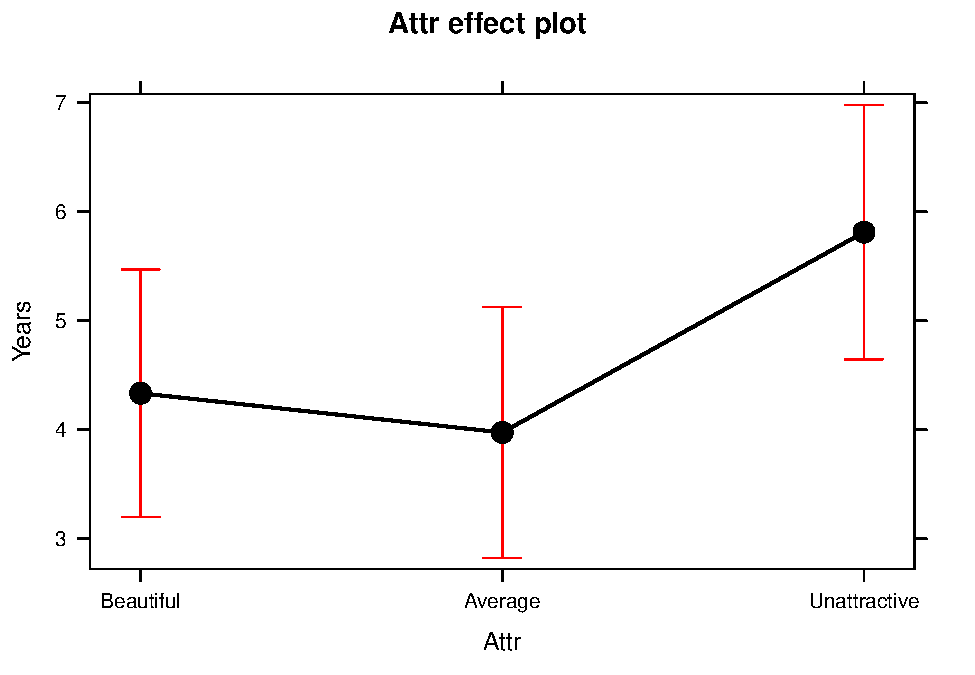
\includegraphics{03-oneWayAnova_files/figure-latex/Figure3-2-1.pdf}
\caption{\label{fig:Figure3-2}Plot of the estimated group mean sentences from the
reference-coded model for the MockJury data.}
\end{figure}

In order to assess evidence for having different means for the groups,
we will compare either of the previous models (cell-means or
reference-coded) to a null model based on the null hypothesis
(\(H_0: \mu_1 = \ldots = \mu_J\)) which implies a model of
\(\color{red}{y_{ij} = \mu_j}+\varepsilon_{ij}\) in the cell-means
version where \({\color{red}{\mu}}\) is a common mean for all the
observations. We will call this the \textcolor{red}{\textbf{mean-only}}
model since it only has a single mean in it. In the reference-coding
version of the model, we have a null hypothesis that
\(H_0: \tau_2 = \ldots = \tau_J = 0\), so the ``mean-only'' model is
\(\color{purple}{y_{ij} =\boldsymbol{\alpha}+\varepsilon_{ij}}\) with
\(\color{purple}{\boldsymbol{\alpha}}\) having the same definition as
\(\color{red}{\mu}\) for the cell means model -- it forces a common
value for the mean for all the groups. Moving from the
\emph{reference-coded} model to the \emph{mean-only} model is also an
example of a situation where we move from a ``full'' model to a
``reduced'' model by setting some coefficients in the ``full'' model to
0 and, by doing this, get a simpler or ``reduced'' model. Simple models
can be good as they are easier to groups that suggests no difference in
the groups is not a very exciting result in most, but not all,
situations\footnote{Suppose we were doing environmental monitoring and
  were studying asbestos levels in soils. We might be hoping that the
  mean-only model were reasonable to use if the groups being compared
  were in remediated areas and in areas known to have never been
  contaminated.}. In order for R to provide results for the mean-only
model, we remove the grouping variable, \texttt{Attr}, from the model
formula and just include a ``1''. The \texttt{(Intercept)} row of the
output provides the estimate for the mean-only model as a reduced model
from either the cell-means or reference-coded models when we assume that
the mean is the same for all groups:

\begin{Shaded}
\begin{Highlighting}[]
\NormalTok{lm3 <-}\StringTok{ }\KeywordTok{lm}\NormalTok{(Years }\OperatorTok{~}\StringTok{ }\DecValTok{1}\NormalTok{, }\DataTypeTok{data=}\NormalTok{MockJury)}
\KeywordTok{summary}\NormalTok{(lm3)}
\end{Highlighting}
\end{Shaded}

\begin{verbatim}
## $coefficients
##             Estimate Std. Error  t value     Pr(>|t|)
## (Intercept) 4.692982  0.3403532 13.78857 5.765681e-26
\end{verbatim}

This model provides an estimate of the common mean for all observations
of \(4.693 = \hat{\mu} = \hat{\alpha}\) years. This value also is the
dashed, horizontal line in the beanplot in Figure \ref{fig:Figure3-1}.
Some people call this mean-only estimate the grand or overall mean.

\section{One-Way ANOVA Sums of Squares, Mean Squares, and
F-test}\label{section3-3}

The previous discussion showed two ways of parameterizing models for the
One-Way ANOVA model and getting estimates from output but still hasn't
addressed how to assess evidence related to whether the observed
differences in the means among the groups is ``real''. In this section,
we develop what is called the \textbf{\emph{ANOVA F-test}} that provides
a method of aggregating the differences among the means of 2 or more
groups and testing our null hypothesis of no difference in the means vs
the alternative. In order to develop the test, some additional notation
is needed. The sample size in each group is denoted \(n_j\) and the
total sample size is
\(\boldsymbol{N=\Sigma n_j = n_1 + n_2 + \ldots + n_J}\) where
\(\Sigma\) (capital sigma) means ``add up over whatever follows''. An
estimated \textbf{\emph{residual}} (\(e_{ij}\)) is the difference
between an observation, \(y_{ij}\), and the model estimate,
\(\hat{y}_{ij} = \hat{\mu}_j\), for that observation,
\(y_{ij}-\hat{y}_{ij} = e_{ij}\). It is basically what is left over that
the mean part of the model (\(\hat{\mu}_{j}\)) does not explain. It is
also a window into how ``good'' the model might be.

Consider the four different fake results for a situation with four
groups (\(J=4\)) displayed in Figure \ref{fig:Figure3-3}. Which of the
different results shows the most and least evidence of differences in
the means? In trying to answer this, think about both how different the
means are (obviously important) and how variable the results are around
the mean. These situations were created to have the same means in
Scenarios 1 and 2 as well as matching means in Scenarios 3 and 4. The
variability around the means matches by shading (lighter or darker). In
Scenarios 1 and 2, the differences in the means is smaller than in the
other two results. But Scenario 2 should provide more evidence of what
little difference in present than Scenario 1 because it has less
variability around the means. The best situation for finding group
differences here is Scenario 4 since it has the largest difference in
the means and the least variability around those means. Our test
statistic somehow needs to allow a comparison of the variability in the
means to the overall variability to help us get results that reflect
that Scenario 4 has the strongest evidence of a difference and Scenario
1 would have the least.





\begin{figure}
\centering
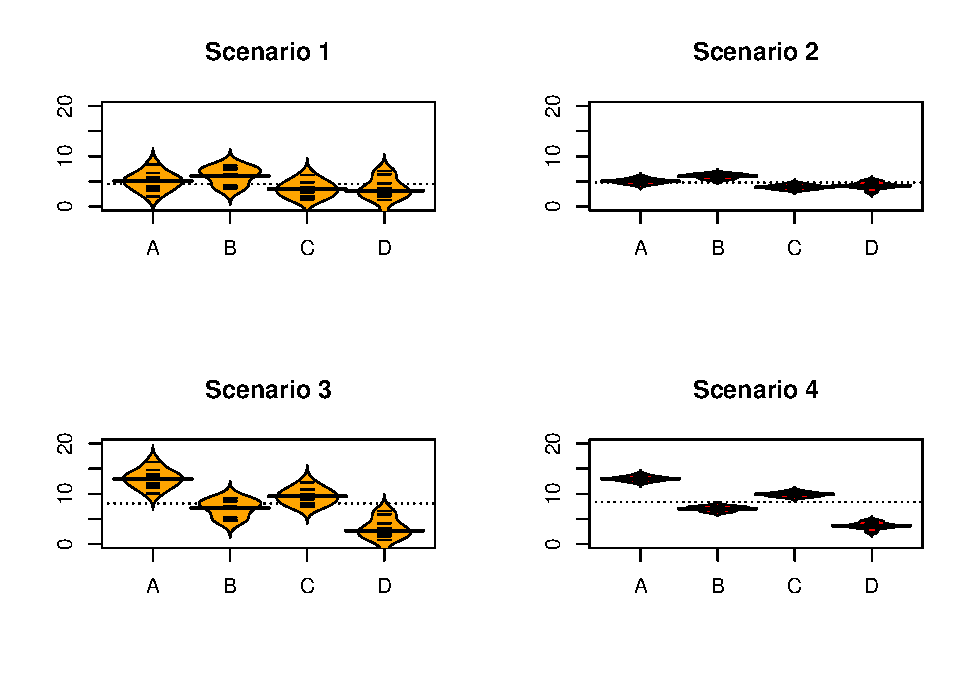
\includegraphics{03-oneWayAnova_files/figure-latex/Figure3-3-1.pdf}
\caption{\label{fig:Figure3-3}Demonstration of different amounts of difference in means
relative to variability. Scenarios have same means in rows and same
variance around means in columns of plot.}
\end{figure}

The statistic that allows the comparison of relative amounts of
variation is called the \textbf{\emph{ANOVA F-statistic}}. It is
developed using \textbf{\emph{sums of squares}} which are measures of
total variation like are used in the numerator of the standard deviation
(\(\Sigma_1^N(y_i-\bar{y})^2\)) that took all the observations,
subtracted the mean, squared the differences, and then added up the
results over all the observations to generate a measure of total
variability. With multiple groups, we will focus on decomposing that
total variability (\textbf{\emph{Total Sums of Squares}}) into
variability among the means (we'll call this \textbf{\emph{Explanatory
Variable}} \(\mathbf{A}\textbf{'s}\) \textbf{\emph{Sums of Squares}})
and variability in the residuals or errors ( \textbf{\emph{Error Sums of
Squares}}). We define each of these quantities in the One-Way ANOVA
situation as follows:

\begin{itemize}
\item
  \(\textbf{SS}_{\textbf{Total}} =\) Total Sums of Squares
  \(= \Sigma^J_{j=1}\Sigma^{n_j}_{i=1}(y_{ij}-\bar{\bar{y}})^2\)

  \begin{itemize}
  \item
    This is the total variation in the responses around the overall or
    \textbf{\emph{grand mean}} (\(\bar{\bar{y}}\), the estimated mean
    for all the observations and available from the mean-only model).
  \item
    By summing over all \(n_j\) observations in each group,
    \(\Sigma^{n_j}_{i=1}(\ )\), and then adding those results up across
    the groups, \(\Sigma^J_{j=1}(\ )\), we accumulate the variation
    across all \(N\) observations.
  \item
    Note: this is the residual variation if the null model is used, so
    there is no further decomposition possible for that model.
  \item
    This is also equivalent to the numerator of the sample variance,
    \(\Sigma^{N}_{1}(y_{i}-\bar{y})^2\) which is what you get when you
    ignore the information on the potential differences in the groups.
  \end{itemize}
\item
  \(\textbf{SS}_{\textbf{A}} =\) Explanatory Variable \emph{A}'s Sums of
  Squares
  \(=\Sigma^J_{j=1}\Sigma^{n_j}_{i=1}(\bar{y}_{i}-\bar{\bar{y}})^2 =\Sigma^J_{j=1}n_j(\bar{y}_{i}-\bar{\bar{y}})^2\)

  \begin{itemize}
  \item
    This is the variation in the group means around the grand mean based
    on the explanatory variable \(A\).
  \item
    Also called sums of squares for the treatment, regression, or model.
  \end{itemize}
\item
  \(\textbf{SS}_E =\) Error (Residual) Sums of Squares
  \(=\Sigma^J_{j=1}\Sigma^{n_j}_{i=1}(y_{ij}-\bar{y})^2 =\Sigma^J_{j=1}\Sigma^{n_j}_{i=1}(e_{ij})^2\)

  \begin{itemize}
  \item
    This is the variation in the responses around the group means.
  \item
    Also called the sums of squares for the residuals, with the second
    version of the formula showing that it is just the squared residuals
    added up across all the observations.
  \end{itemize}
\end{itemize}

The possibly surprising result given the mass of notation just presented
is that the total sums of squares is \textbf{ALWAYS} equal to the sum of
explanatory variable \(A\text{'s}\) sum of squares and the error sums of
squares,

\[\textbf{SS}_{\textbf{Total}} \mathbf{=} \textbf{SS}_\textbf{A} \mathbf{+} \textbf{SS}_\textbf{E}.\]

This equality means that if the \(\textbf{SS}_\textbf{A}\) goes up, then
the \(\textbf{SS}_\textbf{E}\) must go down if
\(\textbf{SS}_{\textbf{Total}}\) remains the same. This result is called
the \textbf{\emph{sums of squares decomposition formula}}. We use these
results to build our test statistic and organize this information in
what is called an \textbf{\emph{ANOVA table}}. The ANOVA table is
generated using the \texttt{anova} function applied to the
reference-coded model, \texttt{lm2} :

\begin{Shaded}
\begin{Highlighting}[]
\NormalTok{lm2<-}\KeywordTok{lm}\NormalTok{(Years }\OperatorTok{~}\StringTok{ }\NormalTok{Attr, }\DataTypeTok{data=}\NormalTok{MockJury)}
\KeywordTok{anova}\NormalTok{(lm2)}
\end{Highlighting}
\end{Shaded}

\begin{verbatim}
## Analysis of Variance Table
## 
## Response: Years
##            Df  Sum Sq Mean Sq F value Pr(>F)
## Attr        2   70.94  35.469    2.77  0.067
## Residuals 111 1421.32  12.805
\end{verbatim}

Note that the ANOVA table has a row labelled \texttt{Attr}, which
contains information for the grouping variable (we'll generally refer to
this as explanatory variable \(A\) but here it is the picture group that
was randomly assigned), and a row labelled \texttt{Residuals}, which is
synonymous with ``Error''. The Sums of Squares (SS) are available in the
\texttt{Sum\ Sq} column. It doesn't show a row for ``Total'' but the
\(\textbf{SS}_{\textbf{Total}} \mathbf{=} \textbf{SS}_\textbf{A} \mathbf{+} \textbf{SS}_\textbf{E} = 1492.26\).

\begin{Shaded}
\begin{Highlighting}[]
\FloatTok{70.94} \OperatorTok{+}\StringTok{ }\FloatTok{1421.32}
\end{Highlighting}
\end{Shaded}

\begin{verbatim}
## [1] 1492.26
\end{verbatim}

It may be easiest to understand the \emph{sums of squares decomposition}
by connecting it to our permutation ideas. In a permutation situation,
the total variation (\(SS_{Total}\)) cannot change -- it is the same
responses varying around the grand mean. However, the amount of
variation attributed to variation among the means and in the residuals
can change if we change which observations go with which group. In
Figure \ref{fig:Figure3-4} (panel a), the means, sums of squares, and
95\% confidence intervals for each mean are displayed for the three
treatment levels from the original prisoner rating data. Three permuted
versions of the data set are summarized in panels (b), (c), and (d). The
\(\text{SS}_A\) is 70.9 in the real data set and between 6.6 and 11 in
the permuted data sets. If you had to pick among the plots for the one
with the most evidence of a difference in the means, you hopefully would
pick panel (a). This visual ``unusualness'' suggests that this observed
result is unusual relative to the possibilities under permutations,
which are, again, the possibilities tied to having the null hypothesis
being true. But note that the differences here are not that great
between these three permuted data sets and the real one. It is likely
that at least some of you might have selected panel (d) as also looking
like it shows some evidence of differences (maybe not the most?) as it
also looks like it shows some evidence differences.

One way to think about \(\textbf{SS}_\textbf{A}\) is that it is a
function that converts the variation in the group means into a single
value. This makes it a reasonable test statistic in a permutation
testing context. By comparing the observed \(\text{SS}_A =\) 70.9 to the
permutation results of 6.5, 9.7, and 40.5 we see that the observed
result is much more extreme than the three alternate versions. In
contrast to our previous test statistics where positive and negative
differences were possible, \(\text{SS}_A\) is always positive with a
value of 0 corresponding to no variation in the means. The larger the
\(\text{SS}_A\), the more variation there is in the means. The
permutation p-value for the alternative hypothesis of \textbf{some} (not
of greater or less than!) difference in the true means of the groups
will involve counting the number of permuted \(SS_A^*\) results that are
larger than what we observed.








\begin{verbatim}
## [1] 70.93836
\end{verbatim}

\begin{figure}
\centering
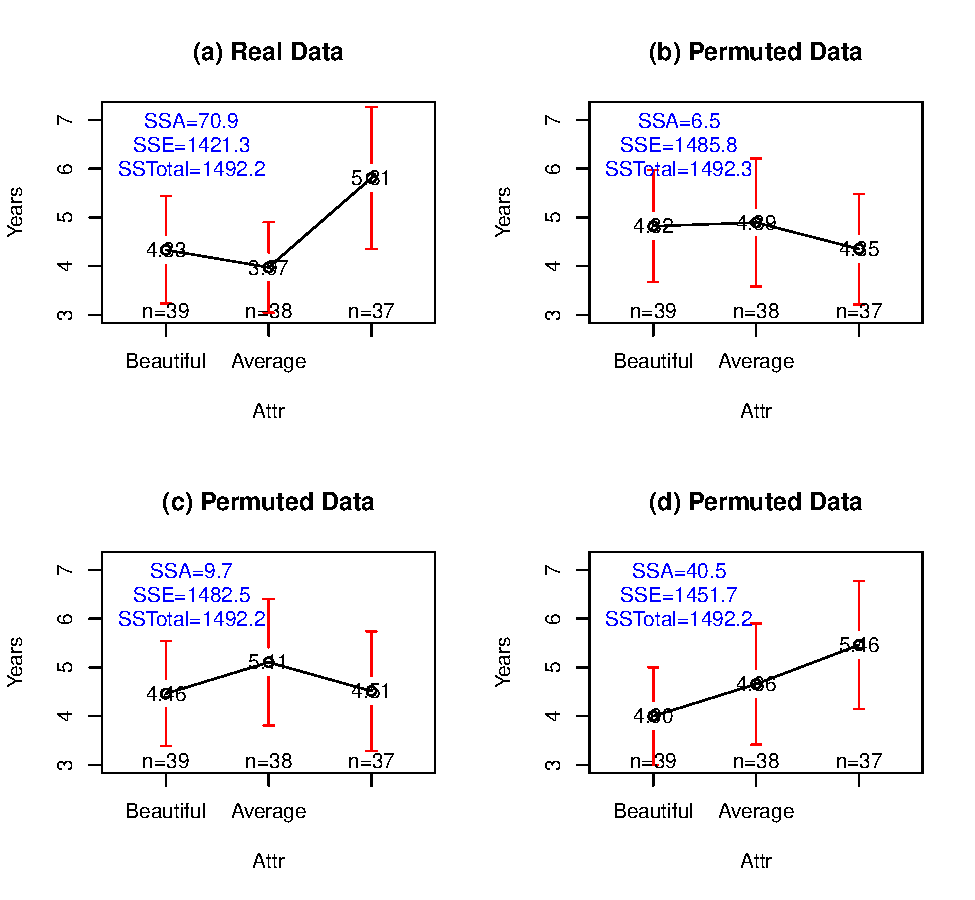
\includegraphics{03-oneWayAnova_files/figure-latex/Figure3-4-1.pdf}
\caption{\label{fig:Figure3-4}Plot of means and 95\% confidence intervals for the three
groups for the real data (a) and three different permutations of the
treatment labels to the same responses in (b), (c), and (d). Note that
SSTotal is always the same but the different amounts of variation
associated with the means (SSA) or the errors (SSE) changes in
permutation.}
\end{figure}

To do a permutation test, we need to be able to calculate and extract
the \(\text{SS}_A\) value. In the ANOVA table, it is in the first row
and is the second number and we can use the bracket, \texttt{{[},\ {]}},
referencing to extract that number from the ANOVA table that
\texttt{anova} produces with
\texttt{anova(lm(Years\textasciitilde{}Attr,\ data=MockJury)){[}1,\ 2{]}}.
We'll store the observed value of \(\text{SS}_A\) in \texttt{Tobs},
reusing some ideas from Chapter \ref{chapter2}.

\begin{Shaded}
\begin{Highlighting}[]
\NormalTok{Tobs <-}\StringTok{ }\KeywordTok{anova}\NormalTok{(}\KeywordTok{lm}\NormalTok{(Years}\OperatorTok{~}\NormalTok{Attr,}\DataTypeTok{data=}\NormalTok{MockJury))[}\DecValTok{1}\NormalTok{,}\DecValTok{2}\NormalTok{]; Tobs}
\end{Highlighting}
\end{Shaded}

\begin{verbatim}
## [1] 70.93836
\end{verbatim}

The following code performs the permutations \texttt{B=1,000} times
using the \texttt{shuffle} function, builds up a vector of results in
\texttt{Tobs}, and then makes a plot of the resulting permutation
distribution:







\begin{Shaded}
\begin{Highlighting}[]
\KeywordTok{par}\NormalTok{(}\DataTypeTok{mfrow=}\KeywordTok{c}\NormalTok{(}\DecValTok{1}\NormalTok{,}\DecValTok{2}\NormalTok{))}
\NormalTok{B<-}\StringTok{ }\DecValTok{1000}
\NormalTok{Tstar<-}\KeywordTok{matrix}\NormalTok{(}\OtherTok{NA}\NormalTok{,}\DataTypeTok{nrow=}\NormalTok{B)}
\ControlFlowTok{for}\NormalTok{ (b }\ControlFlowTok{in}\NormalTok{ (}\DecValTok{1}\OperatorTok{:}\NormalTok{B))\{}
\NormalTok{  Tstar[b]<-}\KeywordTok{anova}\NormalTok{(}\KeywordTok{lm}\NormalTok{(Years}\OperatorTok{~}\KeywordTok{shuffle}\NormalTok{(Attr),}\DataTypeTok{data=}\NormalTok{MockJury))[}\DecValTok{1}\NormalTok{,}\DecValTok{2}\NormalTok{]}
\NormalTok{  \}}
\KeywordTok{hist}\NormalTok{(Tstar,}\DataTypeTok{labels=}\NormalTok{T,}\DataTypeTok{ylim=}\KeywordTok{c}\NormalTok{(}\DecValTok{0}\NormalTok{,}\DecValTok{550}\NormalTok{))}
\KeywordTok{abline}\NormalTok{(}\DataTypeTok{v=}\NormalTok{Tobs,}\DataTypeTok{col=}\StringTok{"red"}\NormalTok{,}\DataTypeTok{lwd=}\DecValTok{3}\NormalTok{)}
\KeywordTok{plot}\NormalTok{(}\KeywordTok{density}\NormalTok{(Tstar),}\DataTypeTok{main=}\StringTok{"Density curve of Tstar"}\NormalTok{)}
\KeywordTok{abline}\NormalTok{(}\DataTypeTok{v=}\NormalTok{Tobs,}\DataTypeTok{col=}\StringTok{"red"}\NormalTok{,}\DataTypeTok{lwd=}\DecValTok{3}\NormalTok{)}
\end{Highlighting}
\end{Shaded}

\begin{figure}
\centering
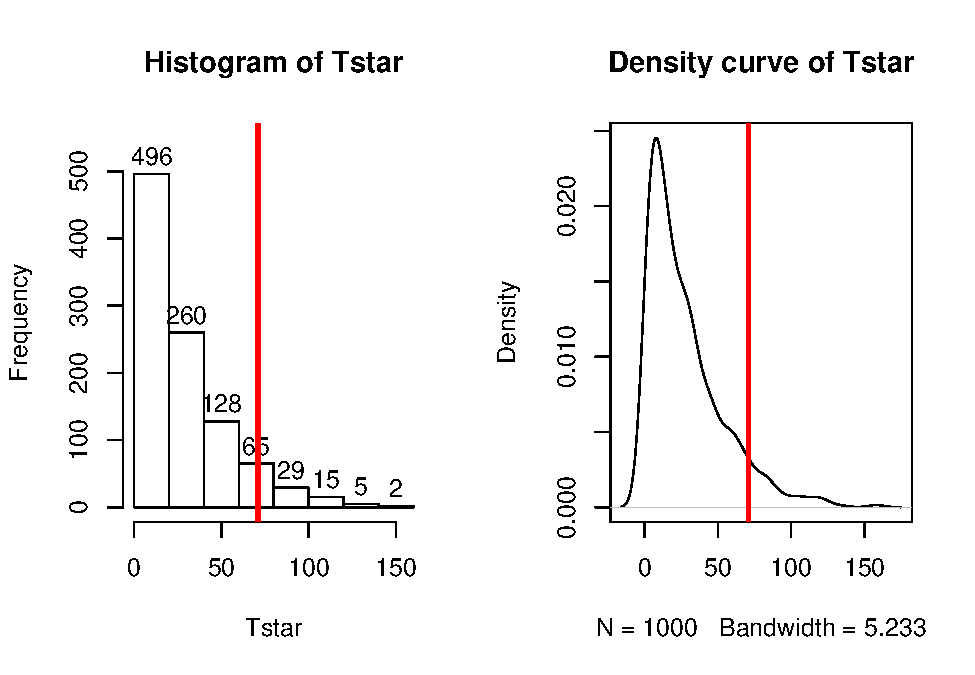
\includegraphics{03-oneWayAnova_files/figure-latex/Figure3-5-1.pdf}
\caption{\label{fig:Figure3-5}Histogram and density curve of permutation distribution of
\(\text{SS}_A\) with the observed value of \(\text{SS}_A\) displayed as
a bold, vertical line. The proportion of results that are larger than
the observed value of \(\text{SS}_A\) provides an estimate of the
p-value.}
\end{figure}

The right-skewed distribution (Figure \ref{fig:Figure3-5}) contains the
distribution of \(\text{SS}_A\text{'s}\) under permutations (where all
the groups are assumed to be equivalent under the null hypothesis).
While the observed result is larger than many of the
\(\text{SS}_A\text{'s}\), there are also many permuted results that are
much larger than observed. The proportion of permuted results that
exceed the observed value is found using \texttt{pdata} as before,
except only for the area to the right of the observed result. We know
that \texttt{Tobs} will always be positive so no absolute values are
required here.

\begin{Shaded}
\begin{Highlighting}[]
\KeywordTok{pdata}\NormalTok{(Tstar,Tobs,}\DataTypeTok{lower.tail=}\NormalTok{F)}
\end{Highlighting}
\end{Shaded}

\begin{verbatim}
## [1] 0.072
\end{verbatim}

This provides a permutation-based p-value of 0.072 and suggests marginal
evidence against the null hypothesis of no difference in the true means.
We would interpret this p-value as saying that there is a 7.2\% chance
of getting a \(\text{SS}_A\) as large or larger than we observed, given
that the null hypothesis is true.

It ends up that some nice parametric statistical results are available
(if our assumptions are met) for the ratio of estimated variances, which
are called \textbf{\emph{Mean Squares}}. To turn sums of squares into
mean square (variance) estimates, we divide the sums of squares by the
amount of free information available. For example, remember the typical
variance estimator introductory statistics,
\(\Sigma^N_1(y_i-\bar{y})^2/(N-1)\)? Your instructor spent some time
trying various approaches to explaining why we have a denominator of
\(N-1\). The most useful for our purposes moving forward is that we
``lose'' one piece of information to estimate the mean and there are
\(N\) deviations around the single mean so we divide by \(N-1\). The
main point is that the sums of squares were divided by something and we
got an estimator for the variance, here of the observations.

Now consider
\(\text{SS}_E = \Sigma^J_{j=1}\Sigma^{n_j}_{i=1}(y_i-\bar{y})^2\) which
still has \(N\) deviations but it varies around the \(J\) means, so the

\[\textbf{Mean Square Error} = \text{MS}_E = \text{SS}_E/(N-J).\]

Basically, we lose \(J\) pieces of information in this calculation
because we have to estimate \(J\) means.

The similar calculation of the \textbf{\emph{Mean Square for variable}}
\(\mathbf{A}\) (\(\text{MS}_A\)) is harder to see in the formula
(\(\text{SS}_A = \Sigma^J_{j=1}n_j(\bar{y}_i-\bar{\bar{y}})^2\)), but
the same reasoning can be used to understand the denominator for forming
\(\text{MS}_A\): there are \(J\) means that vary around the grand mean
so

\[\text{MS}_A = \text{SS}_A/(J-1).\]

In summary, the two mean squares are simply:

\begin{itemize}
\item
  \(\text{MS}_A = \text{SS}_A/(J-1)\), which estimates the variance of
  the group means around the grand mean.
\item
  \(\text{MS}_{\text{Error}} = \text{SS}_{\text{Error}}/(N-J)\), which
  estimates the variation of the errors around the group means.
\end{itemize}

These results are put together using a ratio to define the
\textbf{\emph{ANOVA F-statistic}} (also called the
\textbf{\emph{F-ratio}} ) as

\[F=\text{MS}_A/\text{MS}_{\text{Error}}.\]

If the variability in the means is ``similar'' to the variability in the
residuals, the statistic would have a value around 1. If that
variability is similar then there be no evidence of a difference in the
means. If the \(\text{MS}_A\) is much larger than the \(\text{MS}_E\),
the \(F\)-statistic will provide evidence against the null hypothesis.
The ``size'' of the \(F\)-statistic is formalized by finding the
p-value. The \(F\)-statistic, if assumptions discussed below are met and
we assume the null hypothesis is true, follows what is called an
\(F\)-distribution. The \textbf{\emph{F-distribution}} is a right-skewed
distribution whose shape is defined by what are called the
\textbf{\emph{numerator degrees of freedom}} (\(J-1\)) and the
\textbf{\emph{denominator degrees of freedom}} (\(N-J\)). These names
correspond to the values that we used to calculate the mean squares and
where in the \(F\)-ratio each mean square was used; \(F\)-distributions
are denoted by their degrees of freedom using the convention of \(F\)
(\emph{numerator df}, \emph{denominator df}). Some examples of different
\(F\)-distributions are displayed for you in Figure \ref{fig:Figure3-6}.

The characteristics of the F-distribution can be summarized as:

\begin{itemize}
\item
  Right skewed,
\item
  Nonzero probabilities for values greater than 0,
\item
  Its shape changes depending on the \textbf{numerator} and
  \textbf{denominator DF}, and
\item
  \textbf{Always use the right-tailed area for p-values.}
\end{itemize}






\begin{figure}
\centering
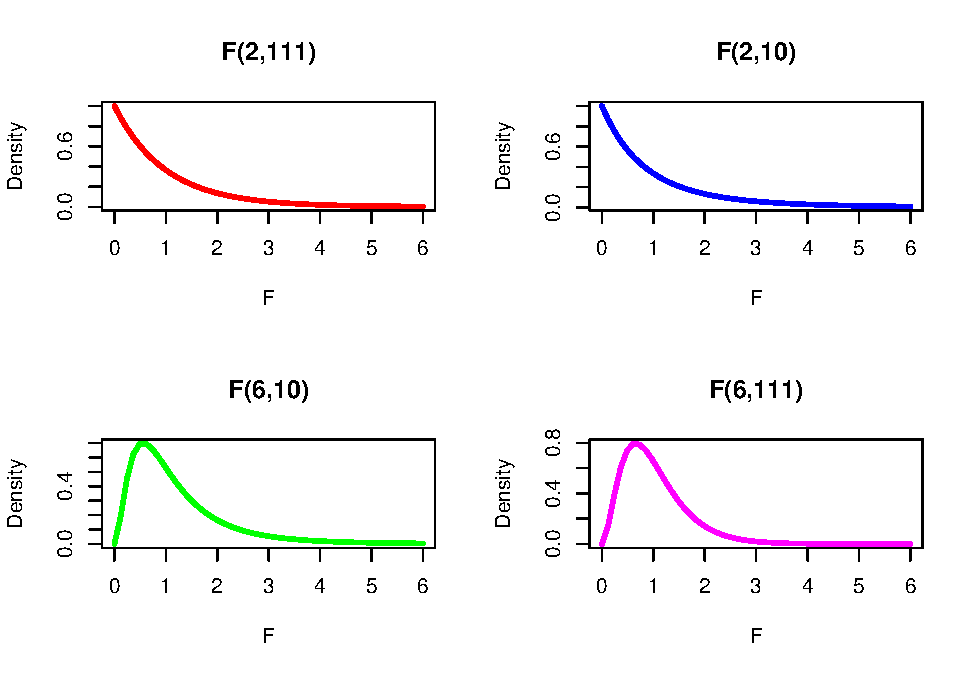
\includegraphics{03-oneWayAnova_files/figure-latex/Figure3-6-1.pdf}
\caption{\label{fig:Figure3-6}Density curves of four different \(F\)-distributions. Upper
left is an \(F(2, 111)\), upper right is \(F(2, 10)\), lower left is
\(F(6, 10)\), and lower right is \(F(6, 111)\). P-values are found using
the areas to the right of the observed \(F\)-statistic value.}
\end{figure}

Now we are ready to discuss an ANOVA table since we know about each of
its components. Note the general format of the ANOVA table is\footnote{Make
  sure you can work from left to right and up and down to fill in the
  ANOVA table given just the necessary information to determine the
  other components -- there is always a question like this on the
  exam\ldots{}}:



\begin{longtable}[]{@{}llllll@{}}
\caption{\label{tab:Table3-2} General One-Way ANOVA table.}\tabularnewline
\toprule
\begin{minipage}[b]{0.09\columnwidth}\raggedright\strut
Source~\strut
\end{minipage} & \begin{minipage}[b]{0.06\columnwidth}\raggedright\strut
DF~\strut
\end{minipage} & \begin{minipage}[b]{0.16\columnwidth}\raggedright\strut
Sums of\\
Squares\strut
\end{minipage} & \begin{minipage}[b]{0.19\columnwidth}\raggedright\strut
Mean Squares\strut
\end{minipage} & \begin{minipage}[b]{0.17\columnwidth}\raggedright\strut
F-ratio\strut
\end{minipage} & \begin{minipage}[b]{0.17\columnwidth}\raggedright\strut
P-value\strut
\end{minipage}\tabularnewline
\midrule
\endfirsthead
\toprule
\begin{minipage}[b]{0.09\columnwidth}\raggedright\strut
Source~\strut
\end{minipage} & \begin{minipage}[b]{0.06\columnwidth}\raggedright\strut
DF~\strut
\end{minipage} & \begin{minipage}[b]{0.16\columnwidth}\raggedright\strut
Sums of\\
Squares\strut
\end{minipage} & \begin{minipage}[b]{0.19\columnwidth}\raggedright\strut
Mean Squares\strut
\end{minipage} & \begin{minipage}[b]{0.17\columnwidth}\raggedright\strut
F-ratio\strut
\end{minipage} & \begin{minipage}[b]{0.17\columnwidth}\raggedright\strut
P-value\strut
\end{minipage}\tabularnewline
\midrule
\endhead
\begin{minipage}[t]{0.09\columnwidth}\raggedright\strut
Variable A\strut
\end{minipage} & \begin{minipage}[t]{0.06\columnwidth}\raggedright\strut
\(J-1\)\strut
\end{minipage} & \begin{minipage}[t]{0.16\columnwidth}\raggedright\strut
\(\text{SS}_A\)\strut
\end{minipage} & \begin{minipage}[t]{0.19\columnwidth}\raggedright\strut
\(\text{MS}_A=\text{SS}_A/(J-1)\)\strut
\end{minipage} & \begin{minipage}[t]{0.17\columnwidth}\raggedright\strut
\(F=\text{MS}_A/\text{MS}_E\)\strut
\end{minipage} & \begin{minipage}[t]{0.17\columnwidth}\raggedright\strut
Right tail of \(F(J-1,N-J)\)\strut
\end{minipage}\tabularnewline
\begin{minipage}[t]{0.09\columnwidth}\raggedright\strut
Residuals\strut
\end{minipage} & \begin{minipage}[t]{0.06\columnwidth}\raggedright\strut
\(N-J\)\strut
\end{minipage} & \begin{minipage}[t]{0.16\columnwidth}\raggedright\strut
\(\text{SS}_E\)\strut
\end{minipage} & \begin{minipage}[t]{0.19\columnwidth}\raggedright\strut
\(\text{MS}_E = \text{SS}_E/(N-J)\)\strut
\end{minipage} & \begin{minipage}[t]{0.17\columnwidth}\raggedright\strut
\strut
\end{minipage} & \begin{minipage}[t]{0.17\columnwidth}\raggedright\strut
\strut
\end{minipage}\tabularnewline
\begin{minipage}[t]{0.09\columnwidth}\raggedright\strut
Total\strut
\end{minipage} & \begin{minipage}[t]{0.06\columnwidth}\raggedright\strut
\(N-1\)\strut
\end{minipage} & \begin{minipage}[t]{0.16\columnwidth}\raggedright\strut
\(\text{SS}_{\text{Total}}\)\strut
\end{minipage} & \begin{minipage}[t]{0.19\columnwidth}\raggedright\strut
\strut
\end{minipage} & \begin{minipage}[t]{0.17\columnwidth}\raggedright\strut
\strut
\end{minipage} & \begin{minipage}[t]{0.17\columnwidth}\raggedright\strut
\strut
\end{minipage}\tabularnewline
\bottomrule
\end{longtable}

The table is oriented to help you reconstruct the \(F\)-ratio from each
of its components. The output from R is similar although it does not
provide the last row and sometimes switches the order of columns. The R
version of the table for the type of picture effect (\texttt{Attr}) with
\(J=3\) levels and \(N=114\) observations, repeated from above, is:

\begin{Shaded}
\begin{Highlighting}[]
\KeywordTok{anova}\NormalTok{(lm2)}
\end{Highlighting}
\end{Shaded}

\begin{verbatim}
## Analysis of Variance Table
## 
## Response: Years
##            Df  Sum Sq Mean Sq F value Pr(>F)
## Attr        2   70.94  35.469    2.77  0.067
## Residuals 111 1421.32  12.805
\end{verbatim}

The p-value from the \(F\)-distribution is 0.067. We can verify this
result using the observed \(F\)-statistic of 2.77 (which came from
taking the ratio of the two mean squares, F=35.47/12.8) which follows an
\(F(2, 111)\) distribution if the null hypothesis is true and some other
assumptions are met.

Using the \texttt{pf} function provides us with areas in the specified
\(F\)-distribution with the \texttt{df1} provided to the function as the
numerator \emph{df} and \texttt{df2} as the denominator \emph{df} and
\texttt{lower.tail=F} reflecting our desire for a right tailed area.

\begin{Shaded}
\begin{Highlighting}[]
\KeywordTok{pf}\NormalTok{(}\FloatTok{2.77}\NormalTok{,}\DataTypeTok{df1=}\DecValTok{2}\NormalTok{,}\DataTypeTok{df2=}\DecValTok{111}\NormalTok{,}\DataTypeTok{lower.tail=}\NormalTok{F)}
\end{Highlighting}
\end{Shaded}

\begin{verbatim}
## [1] 0.06699803
\end{verbatim}

The result from the \(F\)-distribution using this parametric procedure
is similar to the p-value obtained using permutations with the test
statistic of the \(\text{SS}_A\), which was 70.9. The \(F\)-statistic
obviously is another potential test statistic to use as a test statistic
in a permutation approach, now that we know about it. We should check
that we get similar results from it with permutations as we did from
using \(\text{SS}_A\) as a permutation test test statistic. The
following code generates the permutation distribution for the
\(F\)-statistic (Figure \ref{fig:Figure3-7}) and assesses how unusual
the observed \(F\)-statistic of 2.77 was in this permutation
distribution. The only change in the code involves moving from
extracting \(\text{SS}_A\) to extracting the \(F\)-ratio which is in the
4th column of the \texttt{anova} output:

\begin{Shaded}
\begin{Highlighting}[]
\NormalTok{Tobs <-}\StringTok{ }\KeywordTok{anova}\NormalTok{(}\KeywordTok{lm}\NormalTok{(Years }\OperatorTok{~}\StringTok{ }\NormalTok{Attr, }\DataTypeTok{data=}\NormalTok{MockJury))[}\DecValTok{1}\NormalTok{,}\DecValTok{4}\NormalTok{]; Tobs}
\end{Highlighting}
\end{Shaded}

\begin{verbatim}
## [1] 2.770024
\end{verbatim}

\begin{Shaded}
\begin{Highlighting}[]
\KeywordTok{par}\NormalTok{(}\DataTypeTok{mfrow=}\KeywordTok{c}\NormalTok{(}\DecValTok{1}\NormalTok{,}\DecValTok{2}\NormalTok{))}
\NormalTok{B<-}\StringTok{ }\DecValTok{1000}
\NormalTok{Tstar<-}\KeywordTok{matrix}\NormalTok{(}\OtherTok{NA}\NormalTok{,}\DataTypeTok{nrow=}\NormalTok{B)}
\ControlFlowTok{for}\NormalTok{ (b }\ControlFlowTok{in}\NormalTok{ (}\DecValTok{1}\OperatorTok{:}\NormalTok{B))\{}
\NormalTok{  Tstar[b]<-}\KeywordTok{anova}\NormalTok{(}\KeywordTok{lm}\NormalTok{(Years}\OperatorTok{~}\KeywordTok{shuffle}\NormalTok{(Attr), }\DataTypeTok{data=}\NormalTok{MockJury))[}\DecValTok{1}\NormalTok{,}\DecValTok{4}\NormalTok{]}
\NormalTok{\}}

\KeywordTok{pdata}\NormalTok{(Tstar, Tobs, }\DataTypeTok{lower.tail=}\NormalTok{F)}
\end{Highlighting}
\end{Shaded}

\begin{verbatim}
## [1] 0.064
\end{verbatim}

\begin{Shaded}
\begin{Highlighting}[]
\KeywordTok{hist}\NormalTok{(Tstar, }\DataTypeTok{labels=}\NormalTok{T)}
\KeywordTok{abline}\NormalTok{(}\DataTypeTok{v=}\NormalTok{Tobs, }\DataTypeTok{col=}\StringTok{"red"}\NormalTok{, }\DataTypeTok{lwd=}\DecValTok{3}\NormalTok{)}
\KeywordTok{plot}\NormalTok{(}\KeywordTok{density}\NormalTok{(Tstar), }\DataTypeTok{main=}\StringTok{"Density curve of Tstar"}\NormalTok{)}
\KeywordTok{abline}\NormalTok{(}\DataTypeTok{v=}\NormalTok{Tobs, }\DataTypeTok{col=}\StringTok{"red"}\NormalTok{, }\DataTypeTok{lwd=}\DecValTok{3}\NormalTok{)}
\end{Highlighting}
\end{Shaded}





\begin{figure}
\centering
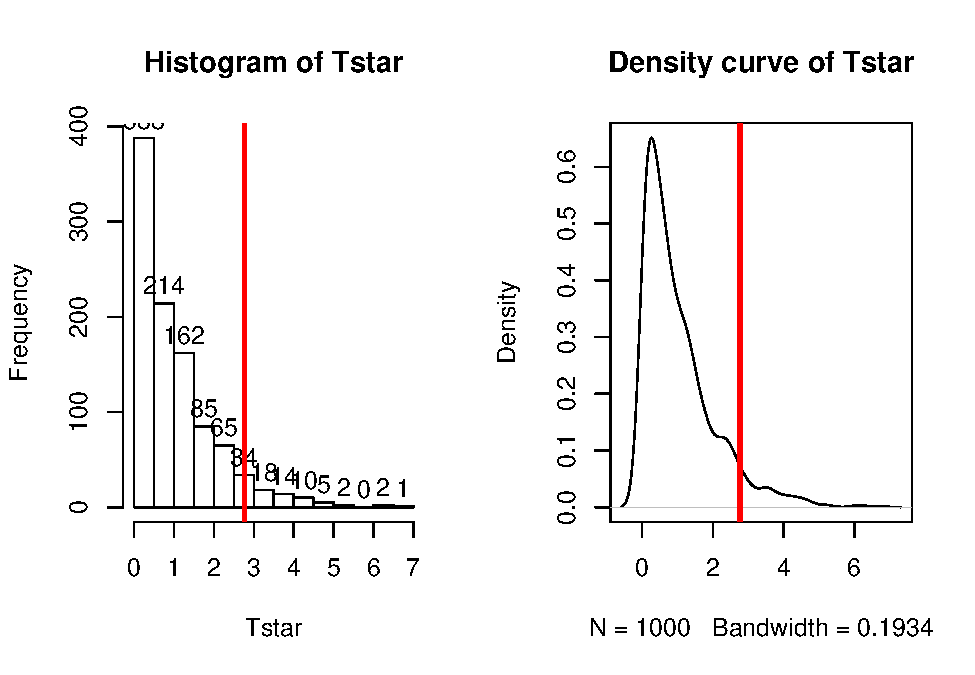
\includegraphics{03-oneWayAnova_files/figure-latex/Figure3-7-1.pdf}
\caption{\label{fig:Figure3-7}Histogram and density curve of the permutation distribution
of the F-statistic with bold, vertical line for observed value of the
test statistic of 2.77.}
\end{figure}

The permutation-based p-value is 0.064 which, again, matches the other
results closely. The first conclusion is that using a test statistic of
either the \(F\)-statistic or the \(\text{SS}_A\) provide similar
permutation results. However, we tend to favor using the \(F\)-statistic
because it is more commonly used in reporting ANOVA results, not because
it is any better in a permutation context.

It is also interesting to compare the permutation distribution for the
\(F\)-statistic and the parametric \(F(2, 111)\) distribution (Figure
\ref{fig:Figure3-8}). They do not match perfectly but are quite similar.
Some the differences around 0 are due to the behavior of the method used
to create the density curve and are not really a problem for the
methods. The similarity in the two curves explains why both methods give
similar results. In some situations, the correspondence will not be
quite so close.




\begin{figure}
\centering
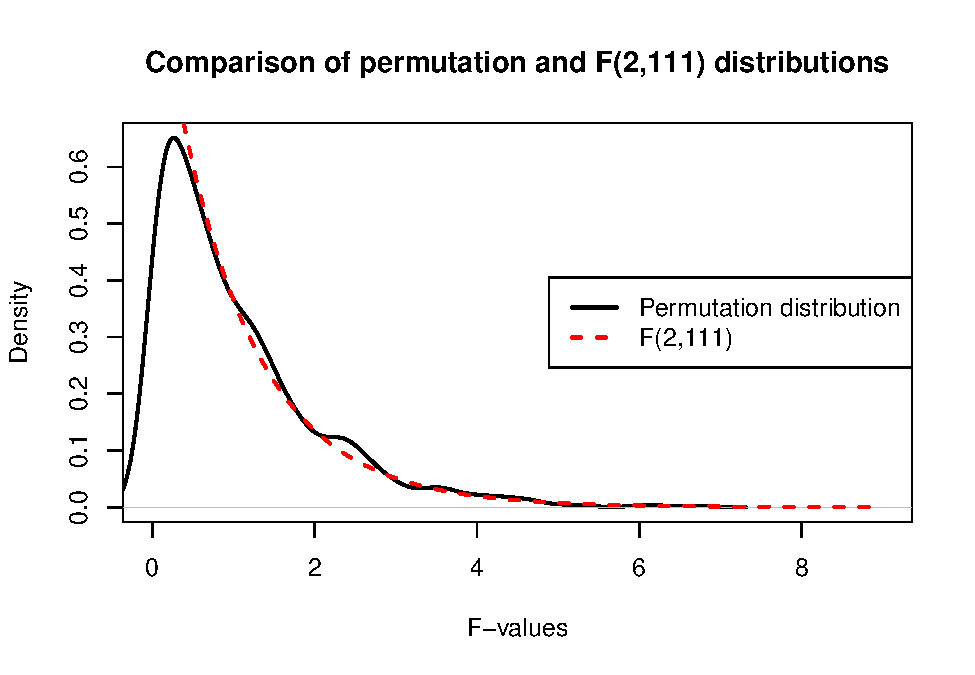
\includegraphics{03-oneWayAnova_files/figure-latex/Figure3-8-1.pdf}
\caption{\label{fig:Figure3-8}Comparison of \(F(2, 111)\) (dashed line) and permutation
distribution (solid line).}
\end{figure}

So how can we rectify this result (\(\text{p-value}\approx 0.06\)) and
the Chapter \ref{chapter2} result that detected a difference between
\emph{Average} and \emph{Unattractive} with a
\(\text{p-value}\approx 0.03\)? I selected the two groups to compare in
Chapter \ref{chapter2} because they were furthest apart.
``Cherry-picking'' the comparison that is likely to be most different
creates a false sense of the real situation and inflates the Type I
error rate because of the selection. If the entire suite of pairwise
comparisons are considered, this result may lose some of its luster. In
other words, if we consider the suite of three pair-wise differences
(and the tests) implicit in comparing all of them, we may need stronger
evidence in the most different pair than a p-value of 0.033 to suggest
overall differences. In this situation, the \emph{Beautiful} and
\emph{Average} groups are not that different from each other so their
difference does not contribute much to the will revisit this topic and
consider a method that is statistically valid for performing all
possible pair-wise comparisons that is also consistent with our overall
test results.

\section{ANOVA model diagnostics including QQ-plots}\label{section3-4}

The requirements for a One-Way ANOVA \(F\)-test are similar to those
discussed in Chapter \ref{chapter2}, except that there are now \(J\)
groups instead of only 2. Specifically, the linear model assumes:

\begin{enumerate}
\def\labelenumi{\arabic{enumi}.}
\item
  \textbf{Independent observations},
\item
  \textbf{Equal variances}, and
\item
  \textbf{Normal distributions}.
\end{enumerate}

For assessing equal variances across the groups, it is best to use plots
to assess this. We can use boxplots and beanplots to compare the spreads
of the groups, which were provided in Figure \ref{fig:Figure3-1}. The
range and IQRs should be relatively similar across the groups if you do
not find evidence of a problem with this assumption. You should start
with noting how clear or big the violation of the assumption might be
but remember that there will always be some differences in the variation
among groups even if the true variability is exactly equal in the
populations. In addition to our direct plotting, there are some
diagnostic plots available from the \texttt{lm} function that can help
us more clearly assess potential violations of the previous assumptions.

We can obtain a suite of four diagnostic plots by using the
\texttt{plot} function on any linear model object that we have fit. To
get all the plots together in four panels we need to add the
\texttt{par(mfrow=c(2,\ 2))} command to tell R to make a graph with 4
panels\footnote{We have been using this function quite a bit to make
  multi-panel graphs but did not show you that line of code. But you
  need to use this command for linear model diagnostics or you won't get
  the plots we want from the model. And you really just need
  \texttt{plot(lm2)} but the \texttt{pch=16} option makes it easier to
  see some of the points in the plots.}.

\begin{Shaded}
\begin{Highlighting}[]
\KeywordTok{par}\NormalTok{(}\DataTypeTok{mfrow=}\KeywordTok{c}\NormalTok{(}\DecValTok{2}\NormalTok{,}\DecValTok{2}\NormalTok{))}
\KeywordTok{plot}\NormalTok{(lm2,}\DataTypeTok{pch=}\DecValTok{16}\NormalTok{)}
\end{Highlighting}
\end{Shaded}

There are two plots in Figure \ref{fig:Figure3-9} with useful
information for the equal variance assumption. The ``Residuals vs
Fitted'' panel in the top left displays the residuals
\((e_{ij} = y_{ij}-\hat{y}_ij)\) on the y-axis and the fitted values
\((\hat{y}_{ij})\) on the x-axis. This allows you to see if the
variability of the observations differs across the groups as a function
of the mean of the groups because all the observations in the same group
get the same fitted value, the mean of the group. In this plot, the
points seem to have fairly similar spreads at the fitted values for the
three groups with fitted values of 4, 4.3, and 6. The ``Scale-Location''
plot in the lower left panel has the same x-axis but the y-axis contains
the square-root of the absolute value of the standardized residuals. The
absolute value transforms all the residuals into a magnitude scale
(removing direction) and the square-root helps you see differences in
variability more accurately. The standardization scales them to have a
variance of 1 so help you in other displays to get a sense of how many
standard deviations you are away from the mean in the residual
distribution. The visual assessment is similar in the two plots -- you
want to consider whether it appears that the groups have somewhat
similar or noticeably different amounts of variability. If you see a
clear funnel shape in the Residuals vs Fitted or an increase or decrease
in the upper edge of points in the Scale-Location plot that may indicate
a violation of the constant variance assumption. Remember that some
variation across the groups is expected and is OK, but large differences
in spreads are problematic for all the procedures that involve linear
models. When discussing these results, you want to discuss how clearly
the differences in variation are and whether that \emph{shows a clear
violation of the assumption} of equal variance for all observations.
Like in hypothesis testing, you can't prove that you've met assumptions
based on a plot ``looking OK'', but you can say that there is no clear
evidence that the assumption is violated!



\begin{figure}
\centering
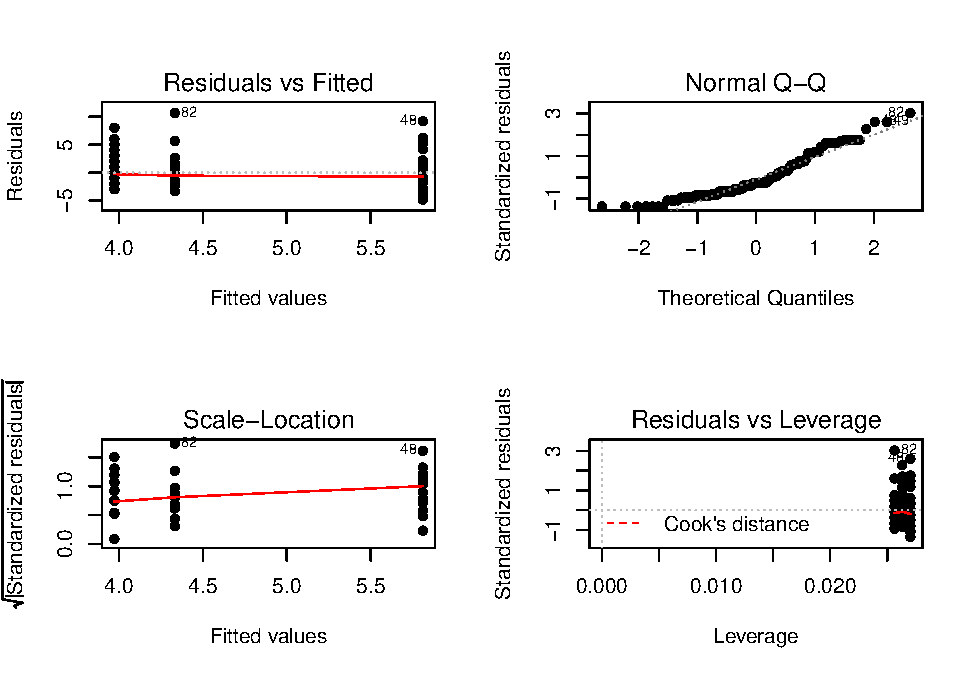
\includegraphics{03-oneWayAnova_files/figure-latex/Figure3-9-1.pdf}
\caption{\label{fig:Figure3-9}Default diagnostic plots for the linear model.}
\end{figure}

The linear model assumes that all the random errors
(\(\varepsilon_{ij}\)) follow a normal distribution. To gain insight
into the validity of this assumption, we can explore the original
observations as displayed in the beanplots, mentally subtracting off the
differences in the means and focusing on the shapes of the distributions
of observations in each group. These plots are especially good for
assessing whether there is there a skew or outliers present in each
group. If so, by definition, the normality assumption is violated. But
our assumption is about the distribution of all the errors after the
remove the differences in the means and so we want an overall assessment
technique to understand how reasonable our assumption is overall for our
model. The residuals from the entire model provide us with estimates of
the random errors and if the normality assumption is met, then the
residuals all-together should approximately follow a normal
distribution. The \textbf{\emph{Normal Q-Q Plot}} in upper right panel
of Figure \ref{fig:Figure3-9} is a direct visual assessment of how well
our residuals match what we would expect from a normal distribution.
Outliers, skew, heavy and light-tailed aspects of distributions (all
violations of normality) show up in this plot once you learn to read it
-- which is our next task. To make it easier to read QQ-plots, it is
nice to start with just considering histograms and/or density plots of
the residuals and to see how that maps into this new display. We can
obtain the residuals from the linear model using the \texttt{residuals}
function on any linear model object.




\begin{Shaded}
\begin{Highlighting}[]
\KeywordTok{par}\NormalTok{(}\DataTypeTok{mfrow=}\KeywordTok{c}\NormalTok{(}\DecValTok{1}\NormalTok{,}\DecValTok{2}\NormalTok{))}
\NormalTok{eij<-}\KeywordTok{residuals}\NormalTok{(lm2)}
\KeywordTok{hist}\NormalTok{(eij, }\DataTypeTok{main=}\StringTok{"Histogram of residuals"}\NormalTok{,}\DataTypeTok{cex.main=}\FloatTok{0.75}\NormalTok{)}
\KeywordTok{plot}\NormalTok{(}\KeywordTok{density}\NormalTok{(eij), }\DataTypeTok{main=}\StringTok{"Density plot of residuals"}\NormalTok{, }\DataTypeTok{ylab=}\StringTok{"Density"}\NormalTok{,}
     \DataTypeTok{xlab=}\StringTok{"Residuals"}\NormalTok{,}\DataTypeTok{cex.main=}\FloatTok{0.75}\NormalTok{)}
\end{Highlighting}
\end{Shaded}

\begin{figure}
\centering
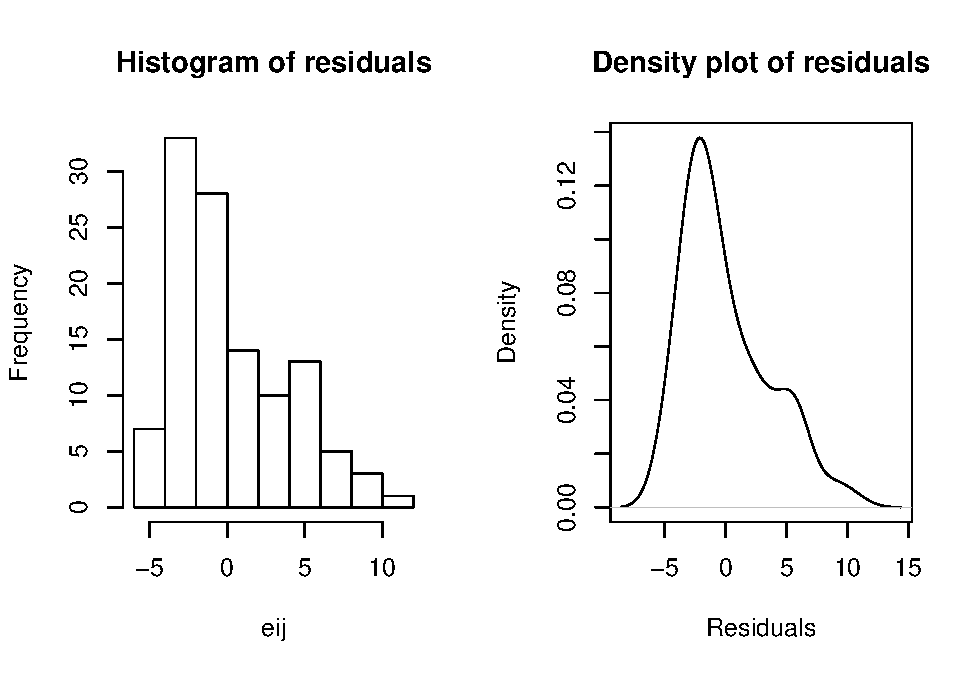
\includegraphics{03-oneWayAnova_files/figure-latex/Figure3-10-1.pdf}
\caption{\label{fig:Figure3-10}Histogram and density curve of the linear model raw
residuals.}
\end{figure}

Figure \ref{fig:Figure3-10} shows that there is a right skew present in
the residuals for the prisoner rating data model that accounted for
different means in the three groups, which is consistent with the
initial assessment of some right skew in the plots of observations in
each group.

A Quantile-Quantile plot (\textbf{\emph{QQ-plot}}) shows the ``match''
of an observed distribution with a theoretical distribution, almost
always the normal distribution. They are also known as Quantile
Comparison, Normal Probability, or Normal Q-Q plots, with the last two
names being specific to comparing results to a normal distribution. In
this version\footnote{Along with multiple names, there is variation of
  what is plotted on the x and y axes and the scaling of the values
  plotted, increasing the challenge of interpreting QQ-plots. We are
  consistent about the x and y axis choices but different functions that
  make these plots in R do switch the axes.}, the QQ-plots display the
value of observed percentiles in the residual distribution on the y-axis
versus the percentiles of a theoretical normal distribution on the
x-axis. If the observed \textbf{distribution of the residuals matches
the shape of the normal distribution, then the plotted points should
follow a 1-1 relationship.} If the points follow the displayed straight
line then that suggests that the residuals have a similar shape to a
normal distribution. Some variation is expected around the line and some
patterns of deviation are worse than others for our models, so you need
to go beyond saying ``it does not match a normal distribution''. It is
best to be specific about the type of deviation you are detecting. And
to do that, we need to practice interpreting some QQ-plots.

The QQ-plot of the linear model residuals from Figure
\ref{fig:Figure3-9} is extracted and enhanced it a little to make Figure
\ref{fig:Figure3-11} so we can just focus on it. We know from looking at
the histogram that this is a slightly right skewed distribution. The
QQ-plot places the observed \textbf{\emph{standardized}}\footnote{Here
  this means re-scaled so that they should have similar scaling to a
  standard normal with mean 0 and standard deviation 1. This does not
  change the shape of the distribution but can make outlier
  identification simpler -- having a standardized residual more extreme
  than 5 or -5 would suggest a deviation from normality since we rarely
  see values that many standard deviations from the mean in a normal
  distribution. But mainly focus on the shape of the pattern in the
  QQ-plot.} \textbf{\emph{residuals}} on the y-axis and the theoretical
normal values on the x-axis. The most noticeable deviation from the 1-1
line is in the lower left corner of the plot. These are for the negative
residuals (left tail) and there are many residuals at around the same
value that are a little smaller than -1. If the distribution had
followed the normal distribution here, the points would be on the 1-1
line and there would be some standardized residuals much smaller than
-1.5. So we are not getting as much spread in the smaller residuals as
we would expect in a normal distribution. If you go back to the
histogram you can see that the smallest residuals are all stacked up and
do not spread out like the left tail of a normal distribution should. In
the right tail (positive) residuals, there is also a systematic lifting
from the 1-1 line to larger values in the residuals than the normal
would generate. For example, the point labeled as ``82'' (the 82nd
observation in the data set) has a value of 3 in residuals but should
actually be smaller (maybe 2.5) if the distribution was normal. Put
together, this pattern in the QQ-plot suggests that the left tail is too
compacted (too short) and the right tail is too spread out -- this is
the right skew we identified from the histogram and density curve!



\begin{figure}
\centering
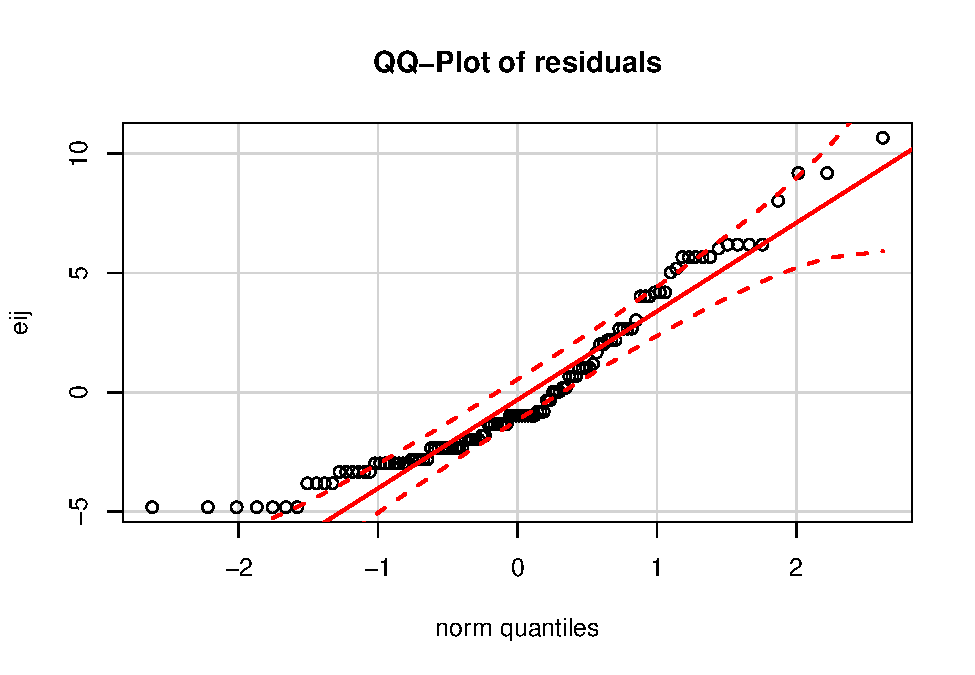
\includegraphics{03-oneWayAnova_files/figure-latex/Figure3-11-1.pdf}
\caption{\label{fig:Figure3-11}QQ-plot of residuals from linear model.}
\end{figure}

Generally, when both tails deviate on the same side of the line (forming
a sort of quadratic curve, especially in more extreme cases), that is
evidence of a skew. To see some different potential shapes in QQ-plots,
six different data sets are displayed in Figures \ref{fig:Figure3-12}
and \ref{fig:Figure3-13}. In each row, a QQ-plot and associated density
curve are displayed. If the points are both above the 1-1 line in the
lower and upper tails as in Figure \ref{fig:Figure3-12}(a), then the
pattern is a right skew, here even more extreme than in the real data
set. If the points are below the 1-1 line in both tails as in Figure
\ref{fig:Figure3-12}(c), then the pattern is identified as a left skew.
Skewed residual distributions (either direction) are problematic for
models that assume normally distributed responses but not necessarily
for our permutation approaches if all the groups have similar skewed
shapes. The other problematic pattern is to have more spread than a
normal curve as in Figure \ref{fig:Figure3-12}(e) and (f). This shows up
with the points being below the line in the left tail (more extreme
negative than expected by the normal) and the points being above the
line for the right tail (more extreme positive than the normal
predicts). We call these distributions \textbf{\emph{heavy-tailed}}
which can manifest as distributions with outliers in both tails or just
a bit more spread out than a normal distribution. Heavy-tailed residual
distributions can be problematic for our models as the variation is
greater than what the normal distribution can account for and our
methods might under-estimate the variability in the results. The
opposite pattern with the left tail above the line and the right tail
below the line suggests less spread (\textbf{\emph{lighter-tailed}})
than a normal as in Figure \ref{fig:Figure3-12}(g) and (h). This pattern
is relatively harmless and you can proceed with methods that assume
normality safely as they will just be a little conservative.




\begin{figure}
\centering
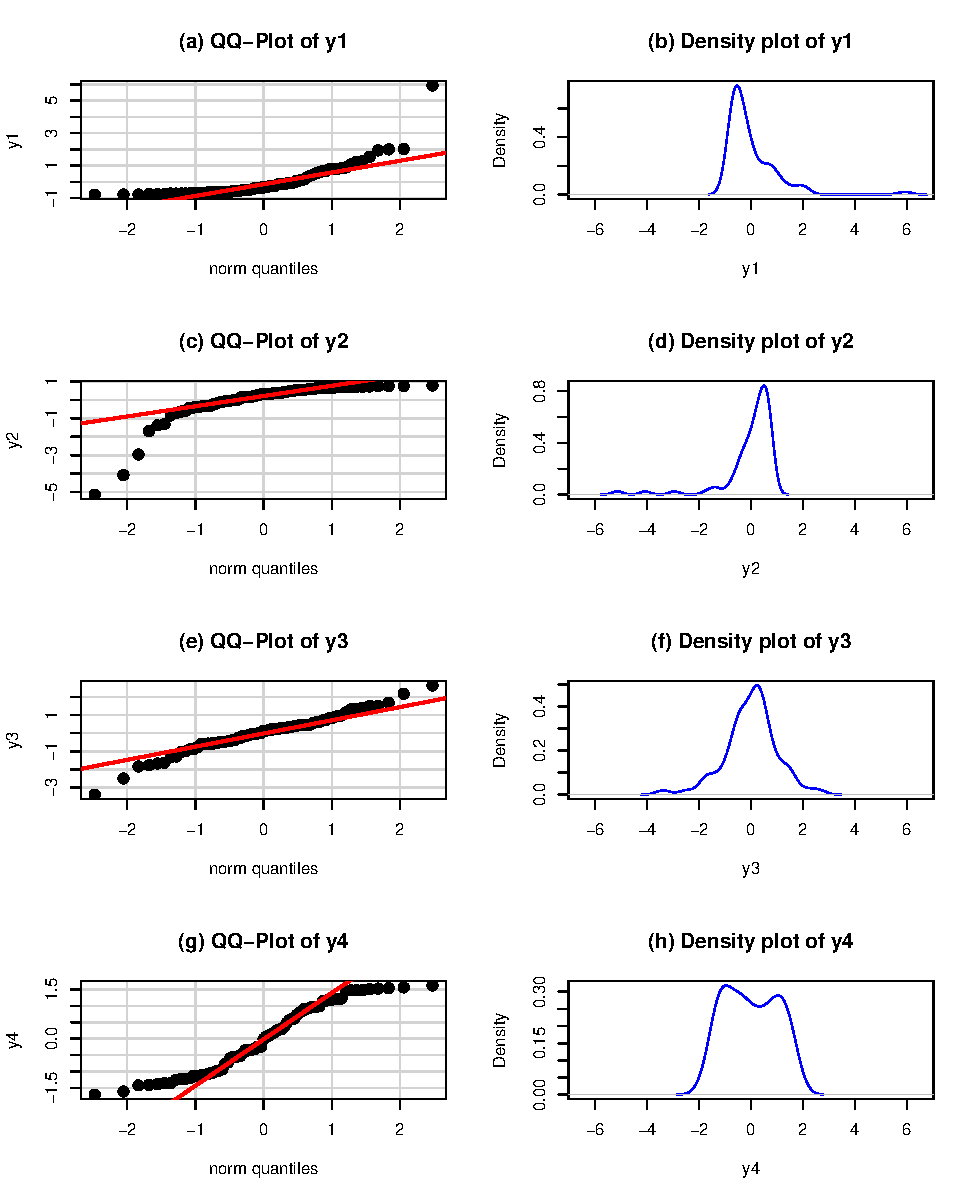
\includegraphics{03-oneWayAnova_files/figure-latex/Figure3-12-1.pdf}
\caption{\label{fig:Figure3-12}QQ-plots and density curves of four simulated
distributions with different shapes.}
\end{figure}

Finally, to help you calibrate expectations for data that are actually
normally distributed, two data sets simulated from normal distributions
are displayed in Figure \ref{fig:Figure3-13}. Note how neither follows
the line exactly but that the overall pattern matches fairly well.
\textbf{You have to allow for some variation from the line in real data
sets} and focus on when there are really noticeable issues in the
distribution of the residuals such as those displayed above. Again, you
will never be able to prove that you have normally distributed residuals
even if the residuals are all exactly on the line, but if you see
QQ-plots as in Figure \ref{fig:Figure3-12} you can encounter situations
that provide evidence of clear violations of the normality assumption.




\begin{figure}
\centering
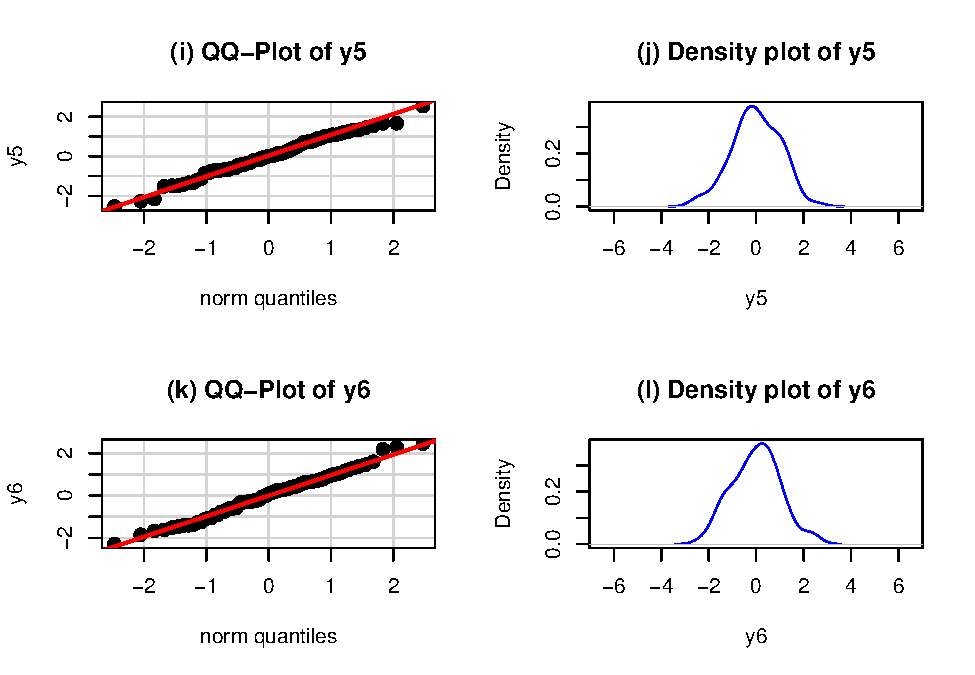
\includegraphics{03-oneWayAnova_files/figure-latex/Figure3-13-1.pdf}
\caption{\label{fig:Figure3-13}Two more simulated data sets, generated from normal
distributions.}
\end{figure}

The last issues with assessing the assumptions in an ANOVA relates to
situations where the methods are more or less
\textbf{\emph{resistant}}\footnote{A resistant procedure is one that is
  not severely impacted by a particular violation of an assumption. For
  example, the median is resistant to the impact of an outlier.} to
violations of assumptions. For reasons beyond the scope of this book,
the parametric ANOVA F-test is more resistant to violations of the
assumptions of the normality and equal variance assumptions if the
design is balanced. A \textbf{\emph{balanced design}} occurs when each
group is measured the same number of times. The resistance decreases as
the data set becomes less balanced, as the sample sizes in the groups
are more different, so having close to balance is preferred to a more
imbalanced situation if there is a choice available. There is some
intuition available here -- it makes some sense that you would have
better results in comparing groups if the information available is
similar in all the groups and none are relatively under-represented. We
can check the number of observations in each group to see if they are
equal or similar using the \texttt{tally} function from the
\texttt{mosaic} package. This function is useful for being able to get
counts of observations, especially for cross-classifying observations on
two variables that is used in Chapter \ref{chapter5}. For just a single
variable, we use \texttt{tally(\textasciitilde{}x,\ data=...)}:

\begin{Shaded}
\begin{Highlighting}[]
\KeywordTok{require}\NormalTok{(mosaic)}
\KeywordTok{tally}\NormalTok{(}\OperatorTok{~}\NormalTok{Attr, }\DataTypeTok{data=}\NormalTok{MockJury)}
\end{Highlighting}
\end{Shaded}

\begin{verbatim}
## Attr
##    Beautiful      Average Unattractive 
##           39           38           37
\end{verbatim}

So the sample sizes do vary among the groups and the design is
technically not balanced, but it is also very close to being balanced
with only two more observations in the largest group compared to the
smallest group size. This tells us that the \(F\)-test should have some
resistance to violations of assumptions. This nearly balanced design,
and the moderate sample size (over 37 per group is considered a good but
not large sample), make the parametric and nonparametric approaches
provide similar results in this data set even in the presence of the
skewed residual error distribution.

\section{Guinea pig tooth growth One-Way ANOVA
example}\label{section3-5}

A second example of the One-way ANOVA methods involves a study of length
of odontoblasts (cells that are responsible for tooth growth) in 60
Guinea Pigs (measured in microns) from \citet{Crampton1947}. \(N=60\)
Guinea Pigs were obtained from a local breeder and each received one of
three dosages (0.5, 1, or 2 mg/day) of Vitamin C via one of two delivery
methods, Orange Juice (\emph{OJ}) or ascorbic acid (the stuff in vitamin
C capsules, called \(VC\) below) as the source of Vitamin C in their
diets. Each guinea pig was randomly assigned to receive one of the six
different treatment combinations possible (OJ at 0.5 mg, OJ at 1 mg, OJ
at 2 mg, VC at 0.5 mg, VC at 1 mg, and VC at 2 mg). The animals were
treated similarly otherwise and we can assume lived in separate cages
and only one observation was taken for each guinea pig, so we can assume
the observations are independent. We need to create a variable that
combines the levels of delivery type (OJ, VC) and the dosages (0.5, 1,
and 2) to use our One-Way ANOVA on the six levels. The
\texttt{interaction} function can be used create a new variable that is
based on combinations of the levels of other variables. Here a new
variable is created in the \texttt{ToothGrowth} data.frame that we
called \texttt{Treat} that provides a six-level grouping variable for
our One-Way ANOVA to compare the combinations of treatments. To get a
sense of the pattern of observations in the data set, the counts in
\texttt{supp} (supplement type) and \texttt{dose} are provided.

\begin{Shaded}
\begin{Highlighting}[]
\KeywordTok{data}\NormalTok{(ToothGrowth) }\CommentTok{#Available in Base R}
\KeywordTok{require}\NormalTok{(mosaic)}
\KeywordTok{tally}\NormalTok{(}\OperatorTok{~}\NormalTok{supp,}\DataTypeTok{data=}\NormalTok{ToothGrowth) }\CommentTok{#Supplement Type (VC or OJ)}
\end{Highlighting}
\end{Shaded}

\begin{verbatim}
## supp
## OJ VC 
## 30 30
\end{verbatim}

\begin{Shaded}
\begin{Highlighting}[]
\KeywordTok{tally}\NormalTok{(}\OperatorTok{~}\NormalTok{dose,}\DataTypeTok{data=}\NormalTok{ToothGrowth) }\CommentTok{#Dosage level}
\end{Highlighting}
\end{Shaded}

\begin{verbatim}
## dose
## 0.5   1   2 
##  20  20  20
\end{verbatim}

\begin{Shaded}
\begin{Highlighting}[]
\CommentTok{#Creates a new variable Treat with 6 levels}
\NormalTok{ToothGrowth}\OperatorTok{$}\NormalTok{Treat=}\KeywordTok{with}\NormalTok{(ToothGrowth,}\KeywordTok{interaction}\NormalTok{(supp,dose)) }

\CommentTok{#New variable that combines supplement type and dosage}
\KeywordTok{tally}\NormalTok{(}\OperatorTok{~}\NormalTok{Treat,}\DataTypeTok{data=}\NormalTok{ToothGrowth) }
\end{Highlighting}
\end{Shaded}

\begin{verbatim}
## Treat
## OJ.0.5 VC.0.5   OJ.1   VC.1   OJ.2   VC.2 
##     10     10     10     10     10     10
\end{verbatim}

The \texttt{tally} function helps us to check for balance; this is a
balanced design because the same number of guinea pigs
(\(n_j=10 \text{ for } j=1, 2,\ldots, 6\)) were measured in each
treatment combination.

With the variable \texttt{Treat} prepared, the first task is to
visualize the results using boxplots and beanplots\footnote{Note that to
  see all the group labels in the plot when making the figure, you have
  to widen the plot window before copying the figure out of R. You can
  resize the plot window using the small vertical and horizontal ``=''
  signs in the grey bars that separate the different panels in RStudio.}
(Figure \ref{fig:Figure3-14}) and generate some summary statistics for
each group using \texttt{favstats}.




\begin{Shaded}
\begin{Highlighting}[]
\KeywordTok{par}\NormalTok{(}\DataTypeTok{mfrow=}\KeywordTok{c}\NormalTok{(}\DecValTok{1}\NormalTok{,}\DecValTok{2}\NormalTok{))}
\KeywordTok{boxplot}\NormalTok{(len}\OperatorTok{~}\NormalTok{Treat,}\DataTypeTok{data=}\NormalTok{ToothGrowth,}\DataTypeTok{ylab=}\StringTok{"Tooth Growth in microns"}\NormalTok{)}
\KeywordTok{beanplot}\NormalTok{(len}\OperatorTok{~}\NormalTok{Treat,}\DataTypeTok{data=}\NormalTok{ToothGrowth,}\DataTypeTok{log=}\StringTok{""}\NormalTok{,}\DataTypeTok{col=}\StringTok{"yellow"}\NormalTok{,}
         \DataTypeTok{method=}\StringTok{"jitter"}\NormalTok{,}\DataTypeTok{ylab=}\StringTok{"Tooth Growth in microns"}\NormalTok{)}
\end{Highlighting}
\end{Shaded}

\begin{figure}
\centering
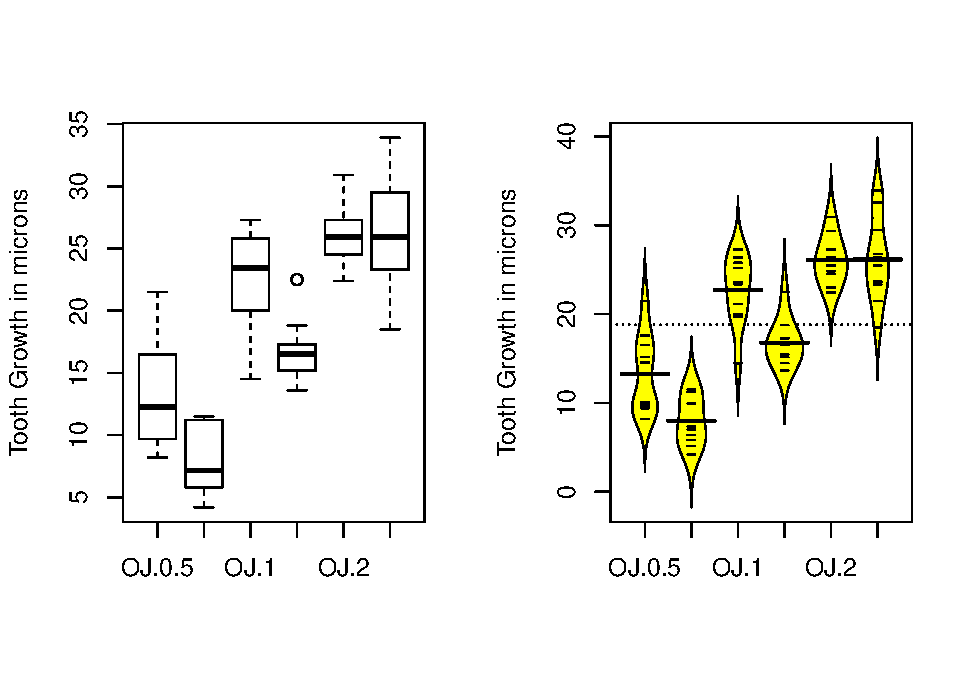
\includegraphics{03-oneWayAnova_files/figure-latex/Figure3-14-1.pdf}
\caption{\label{fig:Figure3-14}Boxplot and beanplot of tooth growth responses for the six
treatment level combinations.}
\end{figure}

\begin{Shaded}
\begin{Highlighting}[]
\KeywordTok{favstats}\NormalTok{(len}\OperatorTok{~}\NormalTok{Treat,}\DataTypeTok{data=}\NormalTok{ToothGrowth)}
\end{Highlighting}
\end{Shaded}

\begin{verbatim}
##    Treat  min     Q1 median     Q3  max  mean       sd  n missing
## 1 OJ.0.5  8.2  9.700  12.25 16.175 21.5 13.23 4.459709 10       0
## 2 VC.0.5  4.2  5.950   7.15 10.900 11.5  7.98 2.746634 10       0
## 3   OJ.1 14.5 20.300  23.45 25.650 27.3 22.70 3.910953 10       0
## 4   VC.1 13.6 15.275  16.50 17.300 22.5 16.77 2.515309 10       0
## 5   OJ.2 22.4 24.575  25.95 27.075 30.9 26.06 2.655058 10       0
## 6   VC.2 18.5 23.375  25.95 28.800 33.9 26.14 4.797731 10       0
\end{verbatim}

Figure \ref{fig:Figure3-14} suggests that the mean tooth growth
increases with the dosage level and that OJ might lead to higher growth
rates than VC except at a dosage of 2 mg/day. The variability around the
means looks to be small relative to the differences among the means, so
we should expect a small p-value from our \(F\)-test. The design is
balanced as noted above (\(n_j=10\) for all six groups) so the methods
are some what resistant to impacts from non-normality and non-constant
variance. There is some suggestion of non-constant variance in the plots
but this will be explored further below when we can remove the
difference in the means and combine all the residuals together. There
might be some skew in the responses in some of the groups but there are
only 10 observations per group so skew in the boxplots could be
generated by impacts of very few of the observations.

Now we can apply our 6+ steps for performing a hypothesis test with
these observations. The initial step is deciding on the claim to be
assessed and the test statistic to use. This is a six group situation
with a quantitative response, identifying it as a One-Way ANOVA where we
want to test a null hypothesis that all the groups have the same
population mean, at least to start. We will use a 5\% significance
level.

\begin{enumerate}
\def\labelenumi{\arabic{enumi}.}
\item
  \textbf{Hypotheses}:
  \(\boldsymbol{H_0: \mu_{OJ0.5} = \mu_{VC0.5} = \mu_{OJ1} = \mu_{VC1} = \mu_{OJ2} = \mu_{VC2}} \textbf{ vs }\)
  \(\boldsymbol{H_A:} \textbf{ Not all } \boldsymbol{\mu_j} \textbf{ equal}\)

  \begin{itemize}
  \item
    The null hypothesis could also be written in reference-coding as
    below since OJ.0.5 is chosen as the baseline group (discussed
    below).

    \begin{itemize}
    \tightlist
    \item
      \(\boldsymbol{H_0:\tau_{VC0.5}=\tau_{OJ1}=\tau_{VC1}=\tau_{OJ2}=\tau_{VC2}=0}\)
    \end{itemize}
  \item
    The alternative hypothesis can be left a bit less specific:

    \begin{itemize}
    \tightlist
    \item
      \(\boldsymbol{H_A:} \textbf{ Not all } \boldsymbol{\tau_j} \textbf{ equal 0}\)
    \end{itemize}
  \end{itemize}
\item
  \textbf{Validity conditions}:

  \begin{itemize}
  \item
    Independence:

    \begin{itemize}
    \tightlist
    \item
      This is where the separate cages note above is important. Suppose
      that there were cages that contained multiple animals and they
      competed for food or could share illness or levels of activity.
      The animals in one cage might be systematically different from the
      others and this ``clustering'' of observations would present a
      potential violation of the independence assumption. If the
      experiment had the animals in separate cages, there is no clear
      dependency in the design of the study and we can assume that there
      is no problem with this assumption.
    \end{itemize}
  \item
    Constant variance:

    \begin{itemize}
    \tightlist
    \item
      As noted above, there is some indication of a difference in the
      variability among the groups in the boxplots and beanplots but the
      sample size was small in each group. We need to fit the linear
      model to get the other diagnostic plots to make an overall
      assessment.
    \end{itemize}

\begin{Shaded}
\begin{Highlighting}[]
\NormalTok{m2<-}\KeywordTok{lm}\NormalTok{(len}\OperatorTok{~}\NormalTok{Treat,}\DataTypeTok{data=}\NormalTok{ToothGrowth)}
\KeywordTok{par}\NormalTok{(}\DataTypeTok{mfrow=}\KeywordTok{c}\NormalTok{(}\DecValTok{2}\NormalTok{,}\DecValTok{2}\NormalTok{))}
\KeywordTok{plot}\NormalTok{(m2,}\DataTypeTok{pch=}\DecValTok{16}\NormalTok{)}
\end{Highlighting}
\end{Shaded}

    \begin{figure}
    \centering
    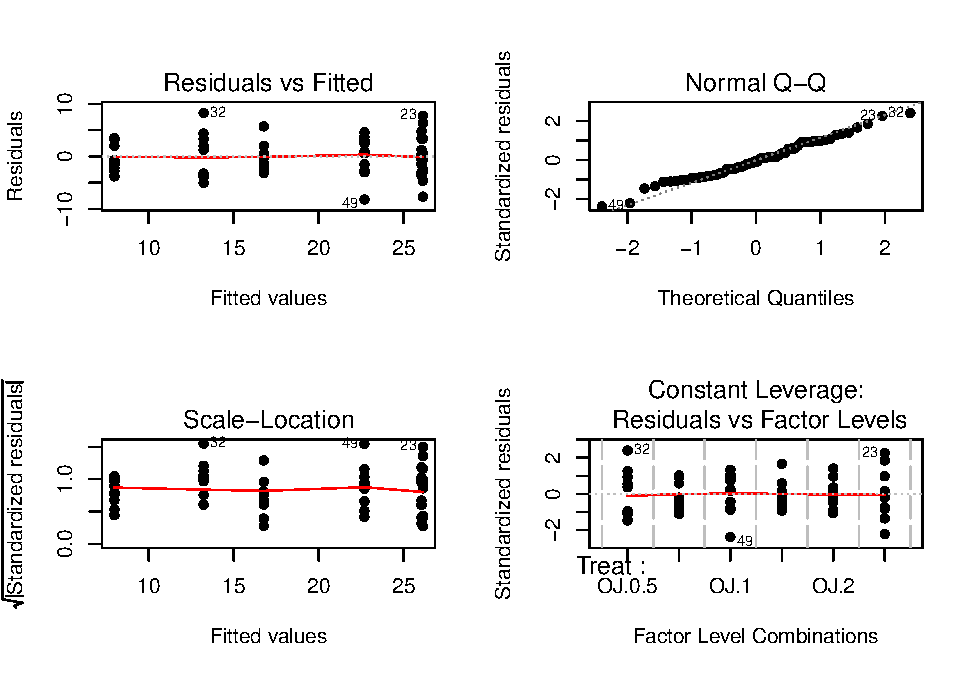
\includegraphics{03-oneWayAnova_files/figure-latex/Figure3-15-1.pdf}
    \caption{\label{fig:Figure3-15}Diagnostic plots for the toothgrowth
    model.}
    \end{figure}

    \begin{itemize}
    \item
      The Residuals vs Fitted panel in Figure \ref{fig:Figure3-15} shows
      some difference in the spreads but the spread is not that
      different between the groups.
    \item
      The Scale-Location plot also shows just a little less variability
      in the group with the smallest fitted value but the spread of the
      groups looks fairly similar in this alternative scaling.
    \item
      Put together, the evidence for non-constant variance is not that
      strong and we can assume that there is at least not a major
      problem with this assumption.
    \end{itemize}
  \item
    Normality of residuals:

    \begin{itemize}
    \tightlist
    \item
      The Normal Q-Q plot shows a small deviation in the lower tail but
      nothing that we wouldn't expect from a normal distribution. So
      there is no evidence of a problem with the normality assumption in
      the upper right panel of Figure \ref{fig:Figure3-15}.
    \end{itemize}
  \end{itemize}
\item
  \textbf{Calculate the test statistic}:

  \begin{itemize}
  \tightlist
  \item
    The ANOVA table for our model follows, providing an \(F\)-statistic
    of 41.557:
  \end{itemize}

\begin{Shaded}
\begin{Highlighting}[]
\KeywordTok{anova}\NormalTok{(m2)}
\end{Highlighting}
\end{Shaded}

\begin{verbatim}
## Analysis of Variance Table
## 
## Response: len
##           Df  Sum Sq Mean Sq F value    Pr(>F)
## Treat      5 2740.10  548.02  41.557 < 2.2e-16
## Residuals 54  712.11   13.19
\end{verbatim}
\item
  \textbf{Find the p-value}:

  \begin{itemize}
  \item
    There are two options here, especially since it seems that our
    assumptions about variance and normality are not violated (note that
    we do not say ``met'' -- we just have no clear evidence against
    them). The parametric and nonparametric approaches should provide
    similar results here.
  \item
    The parametric approach is easiest -- the p-value comes from the
    previous ANOVA table as \texttt{\textless{}2e-16}. First, note that
    this is in scientific notation that is a compact way of saying that
    the p-value here is \(2.2*10^{-16}\) or 0.00000000000000022. When
    you see \texttt{2.2e-16} in R output, it also means that the
    calculation is at the numerical precision of the computer. What R is
    really trying to report is that this is a very small number.
    \textbf{When you encounter p-values that are smaller than 0.0001,
    you should just report that the p-value\textless{}0.0001} Do not
    report that it is 0 as this gives the false impression that there is
    no chance of the result occurring when it is just a really small
    probability. This distribution (the distribution of the test
    statistic if the null hypothesis is true).
  \item
    The nonparametric approach is not too hard so we can compare the two
    approaches here as well:
  \end{itemize}

\begin{Shaded}
\begin{Highlighting}[]
\NormalTok{Tobs <-}\StringTok{ }\KeywordTok{anova}\NormalTok{(}\KeywordTok{lm}\NormalTok{(len}\OperatorTok{~}\NormalTok{Treat,}\DataTypeTok{data=}\NormalTok{ToothGrowth))[}\DecValTok{1}\NormalTok{,}\DecValTok{4}\NormalTok{]; Tobs}
\end{Highlighting}
\end{Shaded}

\begin{verbatim}
## [1] 41.55718
\end{verbatim}

\begin{Shaded}
\begin{Highlighting}[]
\KeywordTok{par}\NormalTok{(}\DataTypeTok{mfrow=}\KeywordTok{c}\NormalTok{(}\DecValTok{1}\NormalTok{,}\DecValTok{2}\NormalTok{))}
\NormalTok{B<-}\StringTok{ }\DecValTok{1000}
\NormalTok{Tstar<-}\KeywordTok{matrix}\NormalTok{(}\OtherTok{NA}\NormalTok{,}\DataTypeTok{nrow=}\NormalTok{B)}
\ControlFlowTok{for}\NormalTok{ (b }\ControlFlowTok{in}\NormalTok{ (}\DecValTok{1}\OperatorTok{:}\NormalTok{B))\{}
\NormalTok{  Tstar[b]<-}\KeywordTok{anova}\NormalTok{(}\KeywordTok{lm}\NormalTok{(len}\OperatorTok{~}\KeywordTok{shuffle}\NormalTok{(Treat),}\DataTypeTok{data=}\NormalTok{ToothGrowth))[}\DecValTok{1}\NormalTok{,}\DecValTok{4}\NormalTok{]}
\NormalTok{\}}
\KeywordTok{pdata}\NormalTok{(Tstar,Tobs,}\DataTypeTok{lower.tail=}\NormalTok{F)}
\end{Highlighting}
\end{Shaded}

\begin{verbatim}
## [1] 0
\end{verbatim}

\begin{Shaded}
\begin{Highlighting}[]
\KeywordTok{hist}\NormalTok{(Tstar,}\DataTypeTok{xlim=}\KeywordTok{c}\NormalTok{(}\DecValTok{0}\NormalTok{,Tobs}\OperatorTok{+}\DecValTok{3}\NormalTok{))}
\KeywordTok{abline}\NormalTok{(}\DataTypeTok{v=}\NormalTok{Tobs,}\DataTypeTok{col=}\StringTok{"red"}\NormalTok{,}\DataTypeTok{lwd=}\DecValTok{3}\NormalTok{)}
\KeywordTok{plot}\NormalTok{(}\KeywordTok{density}\NormalTok{(Tstar),}\DataTypeTok{xlim=}\KeywordTok{c}\NormalTok{(}\DecValTok{0}\NormalTok{,Tobs}\OperatorTok{+}\DecValTok{3}\NormalTok{),}\DataTypeTok{main=}\StringTok{"Density curve of Tstar"}\NormalTok{)}
\KeywordTok{abline}\NormalTok{(}\DataTypeTok{v=}\NormalTok{Tobs,}\DataTypeTok{col=}\StringTok{"red"}\NormalTok{,}\DataTypeTok{lwd=}\DecValTok{3}\NormalTok{)}
\end{Highlighting}
\end{Shaded}

  \begin{figure}
  \centering
  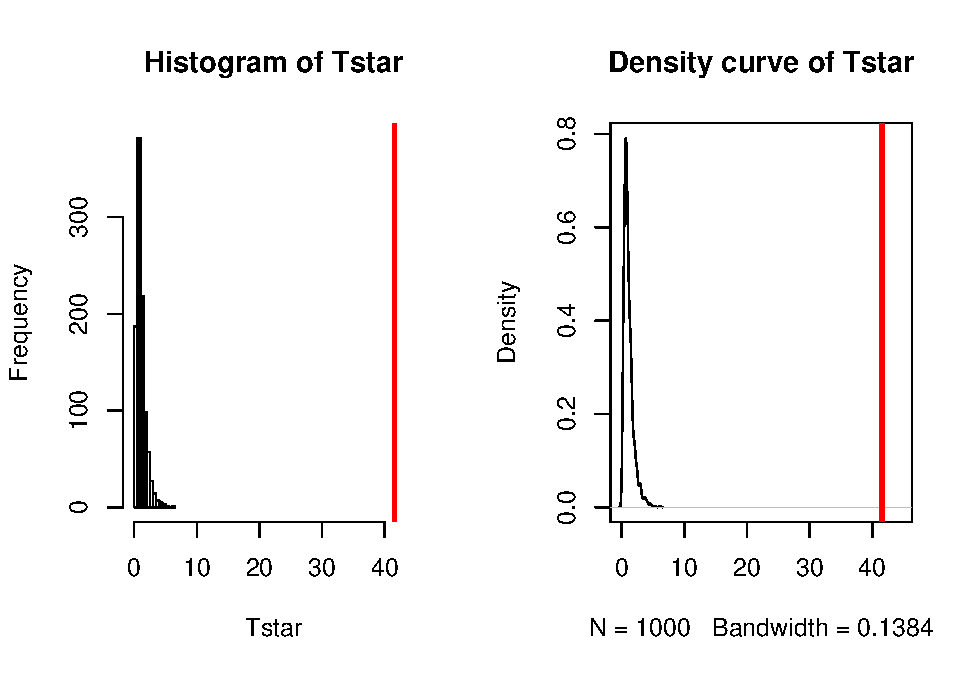
\includegraphics{03-oneWayAnova_files/figure-latex/Figure3-16-1.pdf}
  \caption{\label{fig:Figure3-16}Histogram and density curve of permutation
  distribution for \(F\)-statistic for tooth growth data. Observed test
  statistic in bold, vertical line at 41.56.}
  \end{figure}

  \begin{itemize}
  \tightlist
  \item
    \textbf{The permutation p-value was reported as 0. This should be
    reported as p-value\textless{}0.001} since we did 1000 permutations
    and found that none of the permuted \(F\)-statistics, \(F^*\), were
    larger than the observed \(F\)-statistic of 41.56. The permuted
    results do not exceed 6 as seen in Figure \ref{fig:Figure3-16}, so
    the observed result is \emph{really unusual} relative to the null
    hypothesis. As suggested previously, the parametric and
    nonparametric approaches should be similar here and they were.
  \end{itemize}
\item
  \textbf{Make a decision}:

  \begin{itemize}
  \tightlist
  \item
    Reject \(H_0\) since the p-value is less than 5\%.
  \end{itemize}
\item
  \textbf{Write a conclusion}:

  \begin{itemize}
  \item
    There is evidence at the 5\% significance level that the different
    treatments (combinations of OJ/VC and dosage levels) \textbf{cause
    some} difference in the \textbf{true} mean tooth growth for
    \textbf{these} guinea pigs.

    \begin{itemize}
    \item
      We can make the causal statement of the treatment causing
      differences because the treatments were randomly assigned but
      these inferences only apply to these guinea pigs since they were
      not randomly selected from a larger population.
    \item
      Remember that we are making inferences to the population or true
      means and not the sample means and want to make that clear in any
      conclusion. When there is not a random sample from a population it
      is more natural to discuss the true means since we can't extend to
      the population values.
    \item
      The alternative is that there is some difference in the true means
      -- be sure to make the wording clear that you aren't saying that
      all the means differ. In fact, if you look back at Figure
      \ref{fig:Figure3-14}, the means for the 2 mg dosages look almost
      the same so we will have a tough time arguing that all groups
      differ. The \(F\)-test is about finding evidence of some means.
      The next section will provide some additional tools to get more
      specific about the source of those detected differences.
    \end{itemize}
  \end{itemize}
\end{enumerate}

Before we leave this example, we should revisit our model estimates and
interpretations. The default model parameterization is into the
reference-coding. Running the model \texttt{summary} function on
\texttt{m2} provides the estimated coefficients:

\begin{Shaded}
\begin{Highlighting}[]
\KeywordTok{summary}\NormalTok{(m2)}
\end{Highlighting}
\end{Shaded}

\begin{verbatim}
## 
## Call:
## lm(formula = len ~ Treat, data = ToothGrowth)
## 
## Residuals:
##    Min     1Q Median     3Q    Max 
##  -8.20  -2.72  -0.27   2.65   8.27 
## 
## Coefficients:
##             Estimate Std. Error t value Pr(>|t|)
## (Intercept)   13.230      1.148  11.521 3.60e-16
## TreatVC.0.5   -5.250      1.624  -3.233  0.00209
## TreatOJ.1      9.470      1.624   5.831 3.18e-07
## TreatVC.1      3.540      1.624   2.180  0.03365
## TreatOJ.2     12.830      1.624   7.900 1.43e-10
## TreatVC.2     12.910      1.624   7.949 1.19e-10
## 
## Residual standard error: 3.631 on 54 degrees of freedom
## Multiple R-squared:  0.7937, Adjusted R-squared:  0.7746 
## F-statistic: 41.56 on 5 and 54 DF,  p-value: < 2.2e-16
\end{verbatim}

For some practice with the reference coding used in these models, let's
find the estimates for observations for a couple of the groups. To work
with the parameters, you need to start with diagnosing the baseline
category that was used by considering which level is not displayed in
the output. The \texttt{levels} function can list the groups in a
categorical variable and their coding in the data set. The first level
is usually the baseline category but you should check this in the model
summary as well.

\begin{Shaded}
\begin{Highlighting}[]
\KeywordTok{levels}\NormalTok{(ToothGrowth}\OperatorTok{$}\NormalTok{Treat)}
\end{Highlighting}
\end{Shaded}

\begin{verbatim}
## [1] "OJ.0.5" "VC.0.5" "OJ.1"   "VC.1"   "OJ.2"   "VC.2"
\end{verbatim}

There is a \texttt{VC.0.5} in the second row of the model summary, but
there is no row for \texttt{0J.0.5} and so this must be the baseline
category. That means that the fitted value or model estimate for the OJ
at 0.5 mg/day group is the same as the \texttt{(Intercept)} row or
\(\hat{\alpha}\), estimating a mean tooth growth of 13.23 microns when
the pigs get OJ at a 0.5 mg/day dosage level. You should always start
with working on the baseline level in a reference-coded model. To get
estimates for any other group, then you can use the \texttt{(Intercept)}
estimate and add the deviation for the group of interest. For
\texttt{VC.0.5}, the estimated mean tooth growth is
\(\hat{\alpha} + \hat{\tau}_2 = \hat{\alpha} + \hat{\tau}_{VC0.5}=13.23 + (-5.25)=7.98\)
microns. It is also potentially interesting to directly interpret the
estimated difference (or deviation) between \texttt{OJ0.5} (the
baseline) and \texttt{VC0.5} (group 2) that is
\(\hat{\tau}_{VC0.5}= -5.25\): we estimate that the mean tooth growth in
\texttt{VC0.5} is 5.25 microns shorter than it is in \texttt{OJ0.5}.
This and many other direct comparisons of groups are likely of interest
to researchers involved in studying the impacts of these supplements on
tooth growth and the next section will show us how to do that
(correctly!).

The reference-coding is still going to feel a little uncomfortable so
the comparison to the cell-means model and exploring the effect plot can
help to reinforce that both models patch together the same estimated
means for each group. For example, we can find our estimate of 7.98
microns for the VC0.5 group in the output and Figure
\ref{fig:Figure3-17}. Also note that Figure \ref{fig:Figure3-17} is the
same whether you plot the results from \texttt{m2} or \texttt{m3}.




\begin{Shaded}
\begin{Highlighting}[]
\NormalTok{m3<-}\KeywordTok{lm}\NormalTok{(len}\OperatorTok{~}\NormalTok{Treat}\OperatorTok{-}\DecValTok{1}\NormalTok{,}\DataTypeTok{data=}\NormalTok{ToothGrowth)}
\KeywordTok{summary}\NormalTok{(m3)}
\end{Highlighting}
\end{Shaded}

\begin{verbatim}
## 
## Call:
## lm(formula = len ~ Treat - 1, data = ToothGrowth)
## 
## Residuals:
##    Min     1Q Median     3Q    Max 
##  -8.20  -2.72  -0.27   2.65   8.27 
## 
## Coefficients:
##             Estimate Std. Error t value Pr(>|t|)
## TreatOJ.0.5   13.230      1.148  11.521 3.60e-16
## TreatVC.0.5    7.980      1.148   6.949 4.98e-09
## TreatOJ.1     22.700      1.148  19.767  < 2e-16
## TreatVC.1     16.770      1.148  14.604  < 2e-16
## TreatOJ.2     26.060      1.148  22.693  < 2e-16
## TreatVC.2     26.140      1.148  22.763  < 2e-16
## 
## Residual standard error: 3.631 on 54 degrees of freedom
## Multiple R-squared:  0.9712, Adjusted R-squared:  0.968 
## F-statistic:   303 on 6 and 54 DF,  p-value: < 2.2e-16
\end{verbatim}

\begin{Shaded}
\begin{Highlighting}[]
\KeywordTok{par}\NormalTok{(}\DataTypeTok{mfrow=}\KeywordTok{c}\NormalTok{(}\DecValTok{1}\NormalTok{,}\DecValTok{1}\NormalTok{))}
\KeywordTok{plot}\NormalTok{(}\KeywordTok{allEffects}\NormalTok{(m2))}
\end{Highlighting}
\end{Shaded}

\begin{figure}
\centering
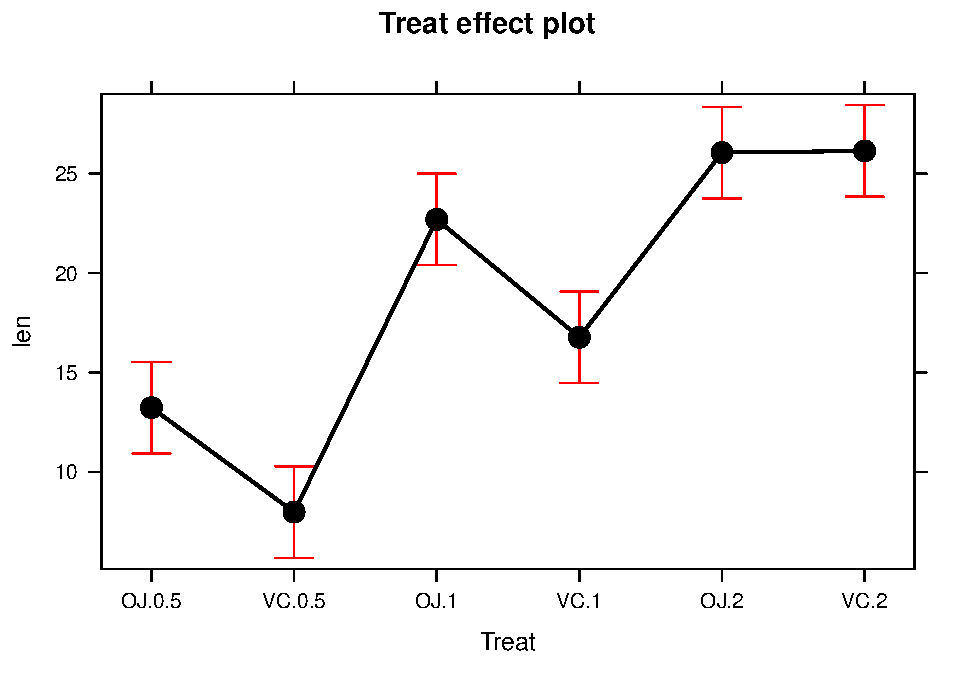
\includegraphics{03-oneWayAnova_files/figure-latex/Figure3-17-1.pdf}
\caption{\label{fig:Figure3-17}Effect plot of the One-Way ANOVA model for the toothgrowth
data.}
\end{figure}

\section{Multiple (pair-wise) comparisons using Tukey's HSD and the
compact letter display}\label{section3-6}

With evidence that the true means are likely not all equal, many
researchers want to know which groups show evidence of differing from
one another. This provides information on the source of the overall
difference that was detected and detailed information on which groups
differed from one another. Because this is a shot-gun/unfocused sort of
approach, some people think it is an over-used procedure. Others feel
that it is an important method of addressing detailed questions about
group comparisons in a valid way. For example, we might want to know if
OJ is dosage level and these methods will allow us to get an answer to
this sort of question. It also will test for differences between the
OJ,0.5 and VC,2 groups and every other pair of levels that you can
construct. This method actually takes us back to the methods in Chapter
\ref{chapter2} where we compared the means of two groups except that we
need to deal with potentially many pair-wise comparisons, making an
adjustment to account for that inflation in Type I errors that occurs
due to many tests being performed at the same time. There are many
different statistical methods to make all the pair-wise comparisons, but
we will employ the most commonly used one, called \textbf{\emph{Tukey's
Honest Significant Difference}} (Tukey's HSD) method\footnote{When this
  procedure is used with unequal group sizes it is also sometimes called
  Tukey-Kramer's method.}. The name suggests that not using it could
lead to a dishonest answer and that it will give you an honest result.
It is more that if you don't do some sort of correction for all the
tests you are performing, you might find some
\textbf{\emph{spurious}}\footnote{We often use ``spurious'' to describe
  falsely rejected null hypotheses, but there are also called false
  detections.} results. There are other methods that could be used to do
a similar correction and also provide ``honest'' inferences; we are just
going to learn one of them.

Generally, the general challenge in this situation is that if you
perform many tests at the same time, you inflate the Type I error rate.
We can define the \textbf{\emph{family-wise error rate}} as the
probability that at least one error is made on a set of tests or, more
compactly, Pr(At least 1 error is made) where Pr() is the probability of
an event occurring. The family-wise error is meant to capture the
overall situation in terms of measuring the likelihood of making a
mistake if we consider many tests, each with some chance of making their
own mistake, and focus on how often we make at least one error when we
do many tests. A quick probability calculation shows the magnitude of
the problem. If we start with a 5\% significance level test, then
Pr(Type I error on one test) =0.05 and the Pr(no errors made on one
test) =0.95, by definition. This is our standard hypothesis testing
situation. Now, suppose we have \(m\) independent tests, then

\[\begin{array}{ll}
& \text{Pr(make at least 1 Type I error given all null hypotheses are true)} \\
& = 1 - \text{Pr(no errors made)} \\
& = 1 - 0.95^m.
\end{array}\]

Figure \ref(fig:Figure3-18) shows how the probability of having at least
one false detection grows rapidly with the number of tests. The plot
stops at 100 tests since it is effectively a 100\% chance of at least on
false detection. It might seem like doing 100 tests is a lot, but in
Genetics research it is possible to consider situations where millions
of tests are considered so these are real issues to be concerned about
in many situations. Researchers want to make sure that when they report
a ``significant'' result that it is really likely to be a real result
and will show up as a difference in the next data set they
collect.\footnote{Many researchers are now collecting multiple data sets
  to use in a single study and using one data set to identify
  interesting results and then using a validation or test data set that
  they withheld from initial analysis to verify that the first results
  are also present in that second data set.}




\begin{figure}
\centering
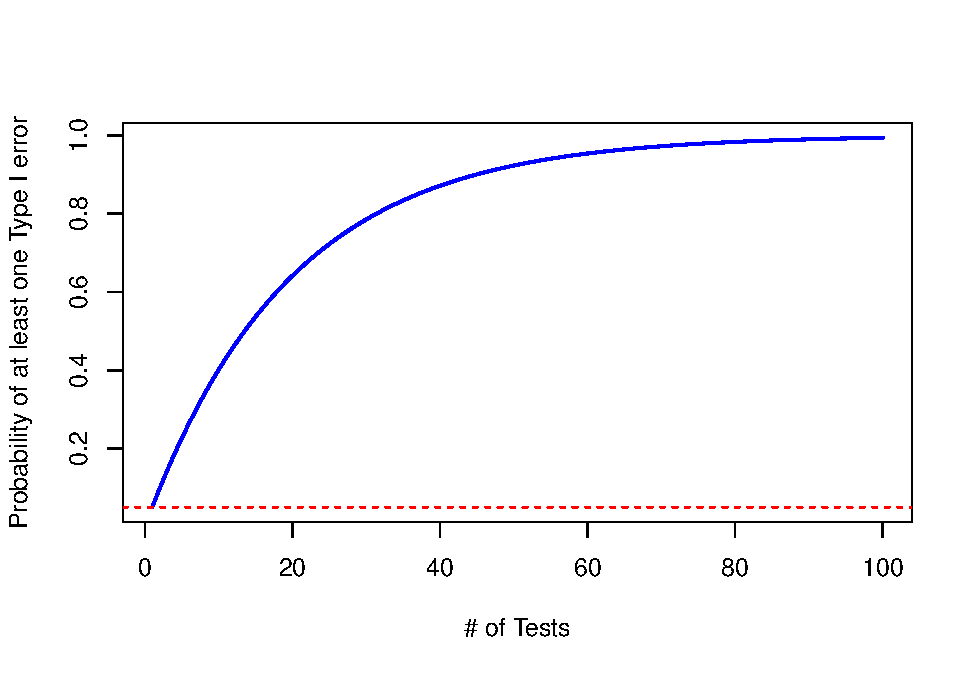
\includegraphics{03-oneWayAnova_files/figure-latex/Figure3-18-1.pdf}
\caption{\label{fig:Figure3-18}Plot of family-wise error rate as the number of tests
performed increases. Dashed line indicates 0.05.}
\end{figure}

In pair-wise comparisons between all the pairs of means in a One-Way
ANOVA, the number of tests is based on the number of pairs. We can
calculate the number of tests using \(J\) choose 2,
\(\begin{pmatrix}J\\2\end{pmatrix}\), to get the number of unique pairs
of size 2 that we can make out of \(J\) individual treatment levels. We
don't need to explore the combinatorics formula for this, as the
\texttt{choose} function can give us the answers:

\begin{Shaded}
\begin{Highlighting}[]
\KeywordTok{choose}\NormalTok{(}\DecValTok{3}\NormalTok{,}\DecValTok{2}\NormalTok{)}
\end{Highlighting}
\end{Shaded}

\begin{verbatim}
## [1] 3
\end{verbatim}

\begin{Shaded}
\begin{Highlighting}[]
\KeywordTok{choose}\NormalTok{(}\DecValTok{4}\NormalTok{,}\DecValTok{2}\NormalTok{)}
\end{Highlighting}
\end{Shaded}

\begin{verbatim}
## [1] 6
\end{verbatim}

\begin{Shaded}
\begin{Highlighting}[]
\KeywordTok{choose}\NormalTok{(}\DecValTok{5}\NormalTok{,}\DecValTok{2}\NormalTok{)}
\end{Highlighting}
\end{Shaded}

\begin{verbatim}
## [1] 10
\end{verbatim}

\begin{Shaded}
\begin{Highlighting}[]
\KeywordTok{choose}\NormalTok{(}\DecValTok{6}\NormalTok{,}\DecValTok{2}\NormalTok{)}
\end{Highlighting}
\end{Shaded}

\begin{verbatim}
## [1] 15
\end{verbatim}

So if you have three groups (prisoner rating study), there are 3 unique
pairs to compare. For six groups, like in the guinea pig study, we have
to consider 15 tests to compare all the unique pairs of groups. 15 tests
seems like enough that we should be worried about inflated family-wise
error rates. Fortunately, the Tukey's HSD method controls the
family-wise error rate at your specified level (say 0.05) across any
number of pair-wise comparisons. This means that the overall rate of at
least one Type I error is controlled at the specified significance
level, often 5\%. To do this, each test must use a slightly more
conservative cut-off than if just one test is performed and the
procedure helps us figure out how much more conservative we need to be.

Tukey's HSD starts with focusing on the difference between the groups
with the largest and smallest means (\(\bar{y}_{max}-\bar{y}_{min}\)).
If \((\bar{y}_{max}-\bar{y}_{min}) \le \text{Margin of Error}\) for the
difference in the means, then all other pairwise differences, say
\(\vert \bar{y}_j - \bar{y}_{j'}\vert\), for two groups \(j\) and
\(j'\), will be less than or equal to that margin of error. This also
means that any confidence intervals for any difference in the means will
contain 0. Tukey's HSD selects a critical value so that
(\(\bar{y}_{max}-\bar{y}_{min}\)) will be less than the margin of error
in 95\% of data sets drawn from populations with a common mean. This
implies that in 95\% of data sets in which all the population means are
the same, all confidence intervals for differences in pairs of means
will contain 0. Tukey's HSD provides confidence intervals for the
difference in true means between groups \(j\) and \(j'\),
\(\mu_j-\mu_{j'}\), for all pairs where \(j \ne j'\), using

\[(\bar{y}_j - \bar{y}_{j'}) \mp \frac{q^*}{\sqrt{2}}\sqrt{\text{MS}_E\left(\frac{1}{n_j}+
\frac{1}{n_{j'}}\right)}\]

where
\(\frac{q^*}{\sqrt{2}}\sqrt{\text{MS}_E\left(\frac{1}{n_j}+ \frac{1}{n_{j'}}\right)}\)
is the margin of error for the intervals. The distribution used to find
the multiplier, \(q^*\), for the confidence intervals is available in
the \texttt{qtukey} function and generally provides a slightly larger
multiplier than the regular \(t^*\) from our two-sample \(t\)-based
confidence interval discussed in Chapter \ref{chapter2}. We will use the
\texttt{confint}, \texttt{cld}, and \texttt{plot} functions applied to
output from the \texttt{glht} function (all from the \texttt{multcomp}
package; \citet{Hothorn2008}, \citep{R-multcomp}) to easily get the
required comparisons from our ANOVA model. Unfortunately, its code
format is a little complicated -- but there are just two places to
modify the code, by including the model name and after \texttt{mcp}
(stands for multiple comparisons) in the \texttt{linfct} option, you
need to include the explanatory variable name as
\texttt{VARIABLENAME="Tukey"}. The last part is to get the TukeyHSD
multiple comparisons run on our explanatory variable. Once we obtain the
intervals, we can use them to test
\(H_0: \mu_j = \mu_{j'} \text{ vs } HA: \mu_j \ne \mu{j'}\) by assessing
whether 0 is in the confidence interval for each pair. If 0 is in the
interval, then there is no evidence of a difference for that pair. If 0
is not in the interval, then we reject \(H_0\) and have evidence
\emph{at the specified family-wise significance level} of a difference
for that pair. You will see a switch to using the word ``detection'' to
describe rejected null hypotheses of no difference as it can help to
write up these results. The following code provides the numerical and
graphical\footnote{The plot of results usually contains all the labels
  of groups but if the labels are long or there many groups, sometimes
  the row labels are hard to see even with re-sizing the plot to make it
  taller in RStudio. The numerical output is useful as a guide to help
  you read the plot.} results of applying Tukey's HSD to the linear
model for the Guinea Pig data:





\begin{Shaded}
\begin{Highlighting}[]
\KeywordTok{par}\NormalTok{(}\DataTypeTok{mfrow=}\KeywordTok{c}\NormalTok{(}\DecValTok{1}\NormalTok{,}\DecValTok{1}\NormalTok{))}
\KeywordTok{require}\NormalTok{(multcomp)}
\NormalTok{Tm2 <-}\StringTok{ }\KeywordTok{glht}\NormalTok{(m2, }\DataTypeTok{linfct =} \KeywordTok{mcp}\NormalTok{(}\DataTypeTok{Treat =} \StringTok{"Tukey"}\NormalTok{))}
\KeywordTok{confint}\NormalTok{(Tm2)}
\end{Highlighting}
\end{Shaded}

\begin{verbatim}
## 
##   Simultaneous Confidence Intervals
## 
## Multiple Comparisons of Means: Tukey Contrasts
## 
## 
## Fit: lm(formula = len ~ Treat, data = ToothGrowth)
## 
## Quantile = 2.9545
## 95% family-wise confidence level
##  
## 
## Linear Hypotheses:
##                      Estimate lwr      upr     
## VC.0.5 - OJ.0.5 == 0  -5.2500 -10.0482  -0.4518
## OJ.1 - OJ.0.5 == 0     9.4700   4.6718  14.2682
## VC.1 - OJ.0.5 == 0     3.5400  -1.2582   8.3382
## OJ.2 - OJ.0.5 == 0    12.8300   8.0318  17.6282
## VC.2 - OJ.0.5 == 0    12.9100   8.1118  17.7082
## OJ.1 - VC.0.5 == 0    14.7200   9.9218  19.5182
## VC.1 - VC.0.5 == 0     8.7900   3.9918  13.5882
## OJ.2 - VC.0.5 == 0    18.0800  13.2818  22.8782
## VC.2 - VC.0.5 == 0    18.1600  13.3618  22.9582
## VC.1 - OJ.1 == 0      -5.9300 -10.7282  -1.1318
## OJ.2 - OJ.1 == 0       3.3600  -1.4382   8.1582
## VC.2 - OJ.1 == 0       3.4400  -1.3582   8.2382
## OJ.2 - VC.1 == 0       9.2900   4.4918  14.0882
## VC.2 - VC.1 == 0       9.3700   4.5718  14.1682
## VC.2 - OJ.2 == 0       0.0800  -4.7182   4.8782
\end{verbatim}

\begin{Shaded}
\begin{Highlighting}[]
\NormalTok{old.par <-}\StringTok{ }\KeywordTok{par}\NormalTok{(}\DataTypeTok{mai=}\KeywordTok{c}\NormalTok{(}\DecValTok{1}\NormalTok{,}\DecValTok{2}\NormalTok{,}\DecValTok{1}\NormalTok{,}\DecValTok{1}\NormalTok{)) }\CommentTok{#Makes room on the plot for the group names}
\KeywordTok{plot}\NormalTok{(Tm2)}
\end{Highlighting}
\end{Shaded}

\begin{figure}
\centering
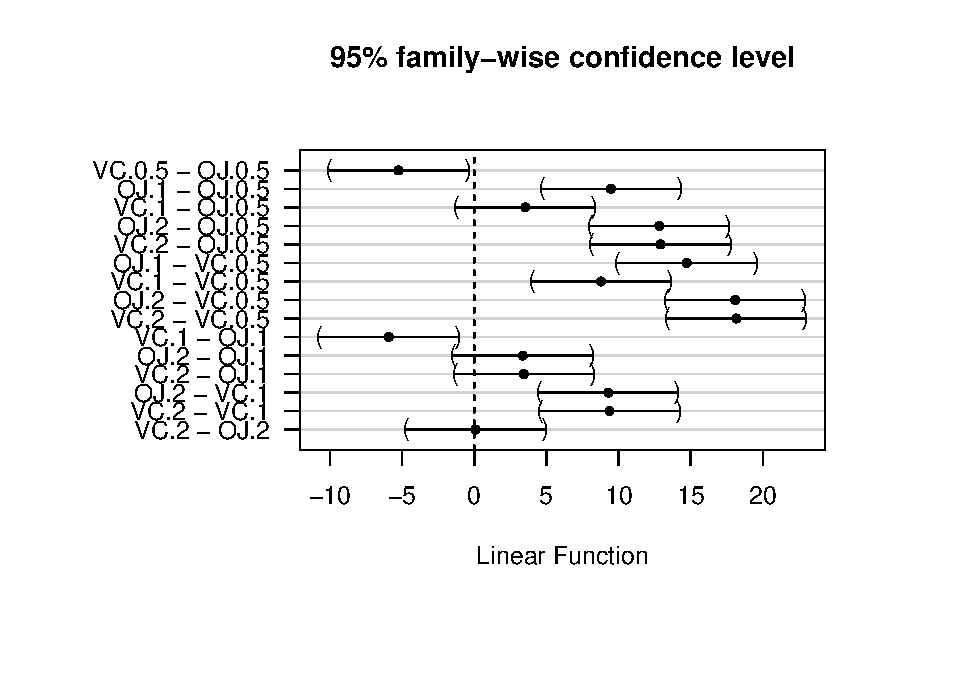
\includegraphics{03-oneWayAnova_files/figure-latex/Figure3-19-1.pdf}
\caption{\label{fig:Figure3-19}Graphical display of pair-wise comparisons from Tukey's
HSD for the Guinea Pig data. Any confidence intervals that do not
contain 0 provide evidence of a difference in the groups.}
\end{figure}

Figure \ref{fig:Figure3-19} contains confidence intervals for the
difference in the means for all 15 pairs of groups. For example, the
first row in the plot contains the confidence interval OJ.0.5). In the
numerical output, you can find that this 95\% family-wise confidence
interval goes from -10.05 to -0.45 microns (\texttt{lwr} and
\texttt{upr} in the numerical output provide the CI endpoints). This
interval does not contain 0 since its upper end point is -0.45 microns
and so we can now say that there is evidence that OJ and VC have
different true mean growth rates at the 0.5 mg dosage level. We can go
further and say that we are 95\% confident that the difference in the
true mean tooth growth between VC.0.5 and OJ.0.5 (VC.0.5-OJ.0.5) is
between -10.05 and -0.45 microns, after adjusting for comparing all the
pairs of groups. But there are fourteen more similar intervals\ldots{}

If you put all these pair-wise tests together, you can generate an
overall interpretation of Tukey's HSD results that discusses sets of
groups that are not detectably different from one another and those
groups that were distinguished from other sets of groups. To do this,
start with listing out the groups that do are not detectably different
(CIs contain 0), which, here, only occurs for four of the pairs. The CIs
that contain 0 are for the pairs VC.1 and OJ.0.5, OJ.2 and OJ.1, VC.2
and OJ.1, and, finally, VC.2 and OJ.2. So VC.2, OJ.1, and OJ.2 are all
not detectably different from each other and VC.1 and OJ.0.5 are also
not detectably different. If you look carefully, VC.0.5 is detected as
different from every other group. So there are basically three sets of
groups that can be grouped together as ``similar'': VC.2, OJ.1, and
OJ.2; VC.1 and OJ.0.5; and VC.0.5. Sometimes groups overlap with some
levels not being detectably different from other levels that belong to
different groups and the story is not as clear as it is in this case. An
example of this sort of overlap is seen in the next section.

There is a method that many researchers use to more efficiently generate
and report these sorts of results that is called a \textbf{\emph{compact
letter display}} (CLD, \citet{Piepho2004}). The \texttt{cld} function
can be applied to the results from \texttt{glht} to generate the CLD
that we can use to provide a ``simple'' summary of the sets of groups.
In this discussion, we define a \textbf{set as a union of different
groups that can contain one or more members} and the member of these
groups are the different treatment levels.

\begin{Shaded}
\begin{Highlighting}[]
\KeywordTok{cld}\NormalTok{(Tm2)}
\end{Highlighting}
\end{Shaded}

\begin{verbatim}
## OJ.0.5 VC.0.5   OJ.1   VC.1   OJ.2   VC.2 
##    "b"    "a"    "c"    "b"    "c"    "c"
\end{verbatim}

Groups with the same letter are not detectably different (are in the
same set) and groups that are detectably different get different letters
(are in different sets). Groups can have more than one letter to reflect
``overlap'' between the sets of groups and sometimes a set of groups
contains only a single treatment level (VC.0.5 is a set of size 1). Note
that if the groups have the same letter, this does not mean they are the
same, just that there is \textbf{no evidence of a difference for that
pair}. If we consider the previous output for the CLD, the ``a'' set
contains VC.0.5, the ``b'' set contains OJ.1, OJ.2, and VC.2, and the
``c'' set contains OJ.0.5 and VC.1. These are exactly the groups of
treatment levels that we obtained by going through all fifteen pairwise
results.

One benefit of this work is that the CLD letters can be added to a
beanplot to help fully report the results and understand the sorts of
differences Tukey's HSD detected.




\begin{figure}
\centering
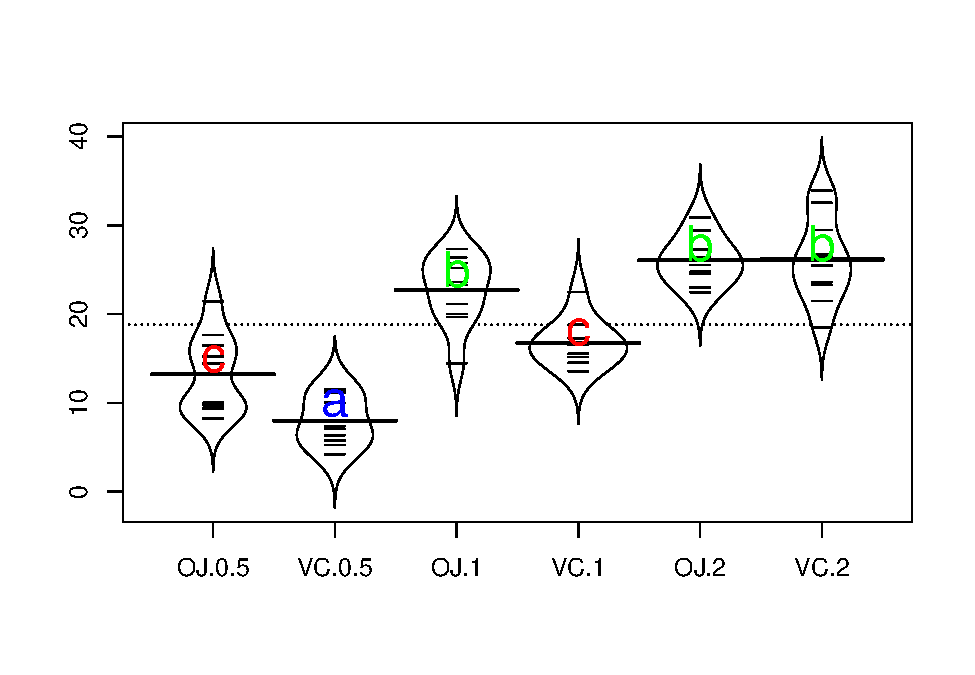
\includegraphics{03-oneWayAnova_files/figure-latex/Figure3-20-1.pdf}
\caption{\label{fig:Figure3-20}Beanplot of tooth growth by group with Tukey's HSD compact
letter display.}
\end{figure}

The lines with text in them are involved in placing text on the figure
but are something you could do in image editing software just as easily.
Figure \ref{fig:Figure3-20} enhances the discussion by showing that the
``\textcolor{blue}{\textbf{a}}'' group with VC.0.5 had the lowest
average tooth growth, the ``\textcolor{red}{\textbf{c}}'' group had
intermediate tooth growth for treatments OJ.0.5 and VC.1, and the
highest growth rates came from OJ.1, OJ.2, and VC.2. Even though VC.2
had the highest average growth rate, we are not able to prove that its
true mean is any higher than the other groups labeled with
``\textcolor{green}{\textbf{b}}''. Hopefully the ease of getting to the
story of the Tukey's HSD results from a plot like this explains why it
is common to report results using these methods instead of reporting 15
confidence intervals.

There are just a couple of other details to mention on this set of
methods. First, note that we interpret the set of confidence intervals
simultaneously: We are 95\% confident that \textbf{ALL} the intervals
contain the respective differences in the true means (this is a
\textbf{\emph{family-wise interpretation}}). These intervals are
adjusted from our regular 2 sample \(t\) intervals from Chapter
\ref{chapter2} to allow this stronger interpretation. Specifically, they
are wider. Second, if sample sizes are unequal in the groups, Tukey's
HSD is conservative and provides a family-wise error rate that is lower
than the nominal (or specified) level. In other words, it fails less
often than expected and the intervals provided are a little wider than
needed, containing all the pairwise differences at higher than the
nominal confidence level of (typically) 95\%. Third, this is a
parametric approach and violations of normality and constant variance
will push the method in the other direction, potentially making the
technique dangerously liberal. Nonparametric approaches to this problem
are also possible, but will not be considered here.

\section{Pair-wise comparisons for Prisoner Rating
data}\label{section3-7}

In our previous work with the prisoner rating data, the overall ANOVA
test provided only marginal evidence of some difference in the true
means across the three groups with a p-value=0.067. Tukey's HSD does not
require you to find a small from your overall \(F\)-test to employ the
methods but if you apply it to situations with p-values larger than your
\emph{a priori} significance level, you are unlikely to find any pairs
that are detected as being different. Some statisticians suggest that
you shouldn't employ follow-up tests such as Tukey's HSD when there is
not sufficient evidence to reject the overall null hypothesis and would
be able to reasonably criticize the following results. But for the sake
of completeness, we can find the pair-wise comparison results at our
typical 95\% family-wise confidence level in this situation, with the
three confidence intervals displayed in Figure \ref{fig:Figure3-21}.




\begin{Shaded}
\begin{Highlighting}[]
\NormalTok{lm2<-}\KeywordTok{lm}\NormalTok{(Years}\OperatorTok{~}\NormalTok{Attr, }\DataTypeTok{data=}\NormalTok{MockJury)}
\KeywordTok{require}\NormalTok{(multcomp)}
\NormalTok{Tm2 <-}\StringTok{ }\KeywordTok{glht}\NormalTok{(lm2, }\DataTypeTok{linfct =} \KeywordTok{mcp}\NormalTok{(}\DataTypeTok{Attr =} \StringTok{"Tukey"}\NormalTok{))}
\KeywordTok{confint}\NormalTok{(Tm2)}
\end{Highlighting}
\end{Shaded}

\begin{verbatim}
## 
##   Simultaneous Confidence Intervals
## 
## Multiple Comparisons of Means: Tukey Contrasts
## 
## 
## Fit: lm(formula = Years ~ Attr, data = MockJury)
## 
## Quantile = 2.3751
## 95% family-wise confidence level
##  
## 
## Linear Hypotheses:
##                               Estimate lwr     upr    
## Average - Beautiful == 0      -0.3596  -2.2969  1.5776
## Unattractive - Beautiful == 0  1.4775  -0.4730  3.4280
## Unattractive - Average == 0    1.8371  -0.1258  3.8001
\end{verbatim}

\begin{Shaded}
\begin{Highlighting}[]
\KeywordTok{cld}\NormalTok{(Tm2)}
\end{Highlighting}
\end{Shaded}

\begin{verbatim}
##    Beautiful      Average Unattractive 
##          "a"          "a"          "a"
\end{verbatim}

\begin{Shaded}
\begin{Highlighting}[]
\NormalTok{old.par <-}\StringTok{ }\KeywordTok{par}\NormalTok{(}\DataTypeTok{mai=}\KeywordTok{c}\NormalTok{(}\DecValTok{1}\NormalTok{,}\FloatTok{2.5}\NormalTok{,}\DecValTok{1}\NormalTok{,}\DecValTok{1}\NormalTok{)) }\CommentTok{#Makes room on the plot for the group names}
\KeywordTok{plot}\NormalTok{(Tm2)}
\end{Highlighting}
\end{Shaded}

\begin{figure}
\centering
\includegraphics{03-oneWayAnova_files/figure-latex/Figure3-21-1.pdf}
\caption{\label{fig:Figure3-21}Tukey's HSD confidence interval results at the 95\%
family-wise confidence level.}
\end{figure}

At the family-wise 5\% significance level, there are no pairs that are
detectably different -- they all get the same letter of ``a''. Now we
will produce results for the reader that thought a 10\% significance was
suitable for this application before seeing any of the results. We just
need to change the confidence level or significance level that the CIs
or tests are produced with inside the functions. For the
\texttt{confint} function, the \texttt{level} option is the confidence
level and for the \texttt{cld}, it is the family-wise significance
level. Note that 90\% confidence corresponds to a 10\% significance
level.



\begin{Shaded}
\begin{Highlighting}[]
\KeywordTok{confint}\NormalTok{(Tm2,}\DataTypeTok{level=}\FloatTok{0.9}\NormalTok{)}
\end{Highlighting}
\end{Shaded}

\begin{verbatim}
## 
##   Simultaneous Confidence Intervals
## 
## Multiple Comparisons of Means: Tukey Contrasts
## 
## 
## Fit: lm(formula = Years ~ Attr, data = MockJury)
## 
## Quantile = 2.0739
## 90% family-wise confidence level
##  
## 
## Linear Hypotheses:
##                               Estimate lwr     upr    
## Average - Beautiful == 0      -0.3596  -2.0513  1.3320
## Unattractive - Beautiful == 0  1.4775  -0.2257  3.1806
## Unattractive - Average == 0    1.8371   0.1231  3.5512
\end{verbatim}

\begin{Shaded}
\begin{Highlighting}[]
\KeywordTok{cld}\NormalTok{(Tm2,}\DataTypeTok{level=}\FloatTok{0.1}\NormalTok{)}
\end{Highlighting}
\end{Shaded}

\begin{verbatim}
##    Beautiful      Average Unattractive 
##         "ab"          "a"          "b"
\end{verbatim}

\begin{Shaded}
\begin{Highlighting}[]
\NormalTok{old.par <-}\StringTok{ }\KeywordTok{par}\NormalTok{(}\DataTypeTok{mai=}\KeywordTok{c}\NormalTok{(}\DecValTok{1}\NormalTok{,}\FloatTok{2.5}\NormalTok{,}\DecValTok{1}\NormalTok{,}\DecValTok{1}\NormalTok{)) }\CommentTok{#Makes room on the plot for the group names}
\KeywordTok{plot}\NormalTok{(}\KeywordTok{confint}\NormalTok{(Tm2,}\DataTypeTok{level=}\NormalTok{.}\DecValTok{9}\NormalTok{))}
\end{Highlighting}
\end{Shaded}

\begin{figure}
\centering
\includegraphics{03-oneWayAnova_files/figure-latex/Figure3-22-1.pdf}
\caption{\label{fig:Figure3-22}Tukey's HSD 90\% family-wise confidence intervals.}
\end{figure}

With family-wise 10\% significance and 90\% confidence levels, the
\emph{Unattractive} and \emph{Average} picture groups are detected as
being different but the \emph{Average} group is not detected as
different from \emph{Beautiful} and \emph{Beautiful} is not detected to
be different from \emph{Unattractive}. This leaves the ``overlap'' of
groups across the sets of groups that was noted earlier. The
\emph{Beautiful} level is not detected as being dissimilar from levels
in two different sets and so gets two different letters.

The beanplot (Figure \ref{fig:Figure3-23}) helps to clarify some of the
reasons for this set of results. The detection of a difference between
\emph{Average} and \emph{Unattractive} just barely occurs and the mean
for \emph{Beautiful} is between the other two so it ends up not being
detectably different from either one. This sort of overlap is actually a
fairly common occurrence in these sorts of situations so be prepared a
mixed set of letters for some levels.







\begin{Shaded}
\begin{Highlighting}[]
\NormalTok{old.par <-}\StringTok{ }\KeywordTok{par}\NormalTok{(}\DataTypeTok{mai=}\KeywordTok{c}\NormalTok{(}\FloatTok{0.5}\NormalTok{,}\DecValTok{1}\NormalTok{,}\DecValTok{1}\NormalTok{,}\DecValTok{1}\NormalTok{))}
\KeywordTok{beanplot}\NormalTok{(Years}\OperatorTok{~}\NormalTok{Attr,}\DataTypeTok{data=}\NormalTok{MockJury,}\DataTypeTok{log=}\StringTok{""}\NormalTok{,}\DataTypeTok{col=}\StringTok{"white"}\NormalTok{,}\DataTypeTok{method=}\StringTok{"jitter"}\NormalTok{)}
\KeywordTok{text}\NormalTok{(}\KeywordTok{c}\NormalTok{(}\DecValTok{1}\NormalTok{),}\KeywordTok{c}\NormalTok{(}\DecValTok{5}\NormalTok{),}\StringTok{"ab"}\NormalTok{,}\DataTypeTok{col=}\StringTok{"blue"}\NormalTok{,}\DataTypeTok{cex=}\FloatTok{1.5}\NormalTok{)}
\KeywordTok{text}\NormalTok{(}\KeywordTok{c}\NormalTok{(}\DecValTok{2}\NormalTok{),}\KeywordTok{c}\NormalTok{(}\FloatTok{4.8}\NormalTok{),}\StringTok{"a"}\NormalTok{,}\DataTypeTok{col=}\StringTok{"green"}\NormalTok{,}\DataTypeTok{cex=}\FloatTok{1.5}\NormalTok{)}
\KeywordTok{text}\NormalTok{(}\KeywordTok{c}\NormalTok{(}\DecValTok{3}\NormalTok{),}\KeywordTok{c}\NormalTok{(}\FloatTok{6.5}\NormalTok{),}\StringTok{"b"}\NormalTok{,}\DataTypeTok{col=}\StringTok{"red"}\NormalTok{,}\DataTypeTok{cex=}\FloatTok{1.5}\NormalTok{)}
\end{Highlighting}
\end{Shaded}

\begin{figure}
\centering
\includegraphics{03-oneWayAnova_files/figure-latex/Figure3-23-1.pdf}
\caption{\label{fig:Figure3-23}Beanplot of sentences with compact letter display results
from 10\% family-wise significance level Tukey's HSD. \emph{Average} and
\emph{Unattractive} picture groups are detected as being different and
are displayed as belonging to different groups. \emph{Beautiful} picture
responses are not detected as different from the other two groups.}
\end{figure}

\section{Chapter Summary}\label{section3-8}

In this chapter, we explored methods for comparing a quantitative
response across \(J\) groups (\(J \ge 2\)), with what is called the
One-Way ANOVA procedure. The initial test is based on assessing evidence
against a null hypothesis of no groups. There are two different methods
for estimating these One-Way ANOVA models: the cell-means model and the
reference-coded versions of the model. There are times when either model
will be preferred, but for the rest of the text, the reference coding is
used (sorry!). The ANOVA \(F\)-statistic, often presented with
underlying information in the ANOVA table, provides a method of
assessing evidence against the null hypothesis either using permutations
or via the \(F\)-distribution. Pair-wise comparisons using Tukey's HSD
provide a method for comparing all the groups and are a nice complement
to the overall ANOVA results. A compact letter display was shown that
enhanced the interpretation of Tukey's HSD result.

In the guinea pig example, we are left with some lingering questions
based on these results. It appears that the effect of \emph{dosage}
changes as a function of the \emph{delivery method} (OJ, VC) because the
size of the differences between OJ and VC change for different dosages.
These methods can't directly assess the question of whether the effect
of delivery method is the same or not across the different dosages. In
chapter \ref{chapter4}, the two variables, \emph{Dosage} and
\emph{Delivery method} are modeled as two separate variables so we can
consider their effects both separately and together. This allows more
refined hypotheses, such as \emph{Is the effect of delivery method the
same for all dosages?}, to be tested. This will introduce new models and
methods for analyzing data where there are two factors as explanatory
variables in a model for a quantitative response variable in what is
called the Two-Way ANOVA.

\section{Summary of important R code}\label{section3-9}

The main components of R code used in this chapter follow with
components to modify in red, remembering that any R packages mentioned
need to be installed and loaded for this code to have a chance of
working:

\begin{itemize}
\item
  \textcolor{red}{MODELNAME} \textless{}-
  lm(\textcolor{red}{Y}\textasciitilde{}\textcolor{red}{X},
  data=\textcolor{red}{DATASETNAME})

  \begin{itemize}
  \item
    Probably the most frequently used command in R.
  \item
    Here it is used to fit the reference-coded One-Way ANOVA model with
    Y as the response variable and X as the grouping variable, storing
    the estimated model object in MODELNAME.
  \end{itemize}
\item
  \textcolor{red}{MODELNAME} \textless{}-
  lm(\textcolor{red}{Y}\textasciitilde{}\textcolor{red}{X}-1,
  data=\textcolor{red}{DATASETNAME})

  \begin{itemize}
  \tightlist
  \item
    Fits the cell means version of the One-Way ANOVA model.
  \end{itemize}
\item
  summary(\textcolor{red}{MODELNAME})

  \begin{itemize}
  \tightlist
  \item
    Generates model summary information including the estimated model
    coefficients, SEs, t-tests, and p-values.
  \end{itemize}
\item
  anova(\textcolor{red}{MODELNAME})

  \begin{itemize}
  \item
    Generates the ANOVA table but \textbf{must only be run on the
    reference-coded version of the model}.
  \item
    Results are incorrect if run on the cell-means model since the
    reduced model under the null is that the mean of all the
    observations is 0!
  \end{itemize}
\item
  pf(\textcolor{red}{FSTATISTIC}, df1=\textcolor{red}{NUMDF},
  df2=\textcolor{red}{DENOMDF}, lower.tail=F)

  \begin{itemize}
  \tightlist
  \item
    Finds the p-value for an observed \(F\)-statistic with NUMDF and
    DENOMDF degrees of freedom.
  \end{itemize}
\item
  par(mfrow=c(2,2)); plot(\textcolor{red}{MODELNAME})

  \begin{itemize}
  \tightlist
  \item
    Generates four diagnostic plots including the Residuals vs Fitted
    and Normal Q-Q plot.
  \end{itemize}
\item
  plot(allEffects(\textcolor{red}{MODELNAME}))

  \begin{itemize}
  \item
    Requires the \texttt{effects} package be loaded.
  \item
    Plots the estimated model component.
  \end{itemize}
\item
  Tm2 \textless{}- glht(\textcolor{red}{MODELNAME},
  linfct=mcp(\textcolor{red}{X}=``Tukey'')); confint(Tm2); plot(Tm2);
  cld(Tm2)

  \begin{itemize}
  \item
    Requires the \texttt{multcomp} package to be installed and loaded.
  \item
    Can only be run on the reference-coded version of the model.
  \item
    Generates the text output and plot for Tukey's HSD as well as the
    compact letter display.
  \end{itemize}
\end{itemize}

\section{Practice problems}\label{section3-10}

For these practice problems, you will work with the cholesterol data set
from the \texttt{multcomp} package that was used to generate the Tukey's
HSD results. To load the data set and learn more about the study, use
the following code:

\begin{verbatim}
require(multcomp)
data(cholesterol)
help(cholesterol)
\end{verbatim}

3.1. Graphically explore the differences in the changes in Cholesterol
levels for the five levels using boxplots and beanplots.

3.2. Is the design balanced?

3.3. Complete all 6+ steps of the hypothesis test using the parametric
\(F\)-test, reporting the ANOVA table and the distribution of the test
statistic under the null.

3.4. Discuss the scope of inference using the information that the
treatment levels were randomly assigned to volunteers in the study.

3.5. Generate the permutation distribution and find the p-value. Compare
the parametric p-value to the permutation test results.

3.6. Perform Tukey's HSD on the data set. Discuss the results -- which
pairs were detected as different and which were not? Bigger reductions
in cholesterol are good, so are there any levels you would recommend or
that might provide similar reductions?

3.7. Find and interpret the CLD and compare that to your interpretation
of results from 3.6.

\chapter{Two-Way ANOVA}\label{chapter4}

\section{Situation}\label{section4-1}

In this chapter, we extend the One-Way ANOVA to situations with two
factors or categorical explanatory variables in a method that is
generally called the \textbf{\emph{Two-Way ANOVA}}. This allows
researchers to simultaneously study more than one variable that might
explain variability in the responses and explore whether the impacts of
one variable change depending on the other variable. In some situations,
each observation is so expensive that researchers want to use a single
study to explore two different sets of research questions in the same
round of data collection. For example, a company might want to study
factors that affect the number of defective products per day and are
interested in the impacts of two different types of training programs
and three different levels of production quotas. These methods would
allow engineers to compare the training programs, production quotas, and
see if the training programs work differently for different production
quotas. In a clinical trials context, it is well known that certain
factors can change the performance of certain drugs. For example,
different dosages of a drug might have different benefits or
side-effects on men, versus women or children. \textbf{When the impact
of one factor changes on the level of another factor}, we say that they
\textbf{\emph{interact}}. It is also possible for both factors to be
related to differences in the mean responses and not interact. For
example, suppose there is a difference in the response means between men
and women and a difference among various dosages, but the effect of
increasing the dosage is the same for the male and female subjects. This
is an example of what is called an \textbf{\emph{additive}} type of
model. In general, the world is more complicated than the single factor
models we considered in Chapter \ref{chapter3} can account for,
especially in observational studies, so these models allow us to start
to handle more realistic situations.

Consider the following ``experiment'' where we want to compare the
strength of different brands of paper towels when they are wet. The
response variable will be the time to failure in seconds (a continuous
response variable) when a weight is placed on the towel held at the four
corners. We are interested in studying the differences between brands
and the impact of different amounts of water applied to the towels.

\begin{itemize}
\item
  Predictors (Explanatory Variables): \textbf{A} : \texttt{Brand} (2
  brands of interest, named \emph{B1} and \emph{B2}) and \textbf{B} :
  Number of \texttt{Drops} of water (10, 20, 30 drops).
\item
  Response: \emph{Time} to failure (in seconds) of a towel (\(y\)) with
  a weight sitting in the middle of the towel.
\end{itemize}

\section{Designing a two-way experiment and visualizing
results}\label{section4-2}

Ideally, we want to randomly assign the levels of each factor so that we
can attribute causality to any detected effects and to reduce the
chances of \emph{confounding}. Because there are two factors, we would
need to design a random assignment scheme to select the levels of both
variables. For example, we could randomly select a brand and then
randomly select the number of drops to apply from the levels chosen for
each measurement. Or we could decide on how many observations we want at
each combination of the two factors (ideally having them all equal so
the design is \textbf{\emph{balanced}}) and then randomize the order of
applying the different combinations of levels.

Why might it be important to randomly apply the brand and number of
drops in an experiment? There are situations where the order of
observations can be related to changes in the responses and we want to
be able to eliminate the order of observations from being related to the
levels of the factors. For example, suppose that the area where the
experiment is being performed becomes wet over time and the later
measurements have extra water that gets onto the paper towels and they
tend to fail more quickly. If all the observations for the second brand
were done later in the study, then the \emph{order of observations}
impacts could make the second brand look worse. If the order of
observations is randomized, then even if there is some drift in the
responses over the order of observations it should still be possible to
see the differences in the randomly assigned effects. If the study
incorporates repeated measurements on human subjects, randomizing the
order of treatments they are exposed to can alleviate impacts of them
``learning'' through the study, something that we would not have to
worry about with paper towels.

In observational studies, we do not have the luxury of random
assignment, that is, we cannot randomly assign levels of the treatment
variables to our subjects, so we cannot guarantee that the only
difference between the groups are the explanatory variables. As
discussed before, because we can't control which level of the variables
are assigned to the subjects, we cannot make causal inferences and have
to worry about other variables being the real drivers of the results.
Although we can never establish causal inference with observational
studies, we can generalize our results to a larger population if we have
a representative sample from our population of interest.

It is also possible that we might have studies where some of the
variables are randomly assigned and others are not randomly assignable.
The most common versions of this are what we sometimes call subject
``demographics'', such as sex, income, race, etc. We might be performing
a study where we can randomly assign treatments to these subjects but
might also want to account for differences based on income level, which
we can't assign. In these cases, the scope of inference gets complicated
-- differences seen on randomized variables can be causally interpreted
but you have to be careful to not say that the demographics caused
differences. Suppose that a randomly assigned drug dosage is found to
show differences in male patients but not in female patients. We could
say that the dosage causes differences in males but does not in females.
We are not saying that sex caused the differences but that the causal
differences were modified by the sex of the subjects.

Even when we do have random assignment of treatments it is important to
think about who/what is included in the sample. To get back to the paper
towel example, we are probably interested in more than the sheets of the
rolls we have to work with so if we could randomly select the studied
paper towels from all paper towels made by each brand, our conclusions
could be extended to those populations. That probably would not be
practical, but trying to make sure that the towels are representative of
all made by each brand by checking for defects and maybe picking towels
from a few different rolls would be a good start to being able to extend
inferences beyond the tested towels.

Once random assignment and random sampling is settled, the final aspect
of study design involves deciding on the number of observations that
should be made. The short (glib) answer is to take as many as you can
afford. With more observations comes higher power to detect differences
if they exist, which is a desired attribute of all studies. It is also
important to make sure that you obtain multiple observations at each
combination of the treatment levels, which are called
\textbf{\emph{replicates}}. Having replicate measurements allows
estimation of the mean for each combination of the treatment levels as
well as estimation and testing for an interaction. And we always prefer
having balanced designs because they provide resistance to violation of
some assumptions as noted in Chapter \ref{chapter3}. A
\textbf{\emph{balanced design}} in a Two-Way ANOVA setting involves
having the same sample size for every combination of the levels of the
treatments.

With two categorical explanatory variables, there are now five possible
scenarios for the truth. Different situations are created depending on
whether there is an interaction between the two variables, whether both
variables are important but do not interact, or whether either of the
variables matter at all. Basically, there are five different possible
outcomes in a randomized Two-Way ANOVA study, listed in order of
increasing model complexity:

\begin{enumerate}
\def\labelenumi{\arabic{enumi}.}
\item
  Neither A or B has an effect on the responses (nothing causes
  differences in responses).
\item
  A has an effect, B does not (only A causes differences in responses).
\item
  B has an effect, A does not (only B causes differences in responses).
\item
  Both A and B have effects on response but no interaction (A and B both
  cause differences in responses but the impacts are additive).
\item
  Effect of A differs based on the levels of B, the opposite is also
  true (means for levels of A are different for different levels of B,
  or, simply, A and B interact).
\end{enumerate}

To illustrate these five potential outcomes, we will consider a fake
version of the paper towel example. It ended up being really messy and
complicated to actually perform the experiment as we described it so
these data were simulated to help us understand the Two-Way ANOVA
possibilities in as simple a situation as possible. The first step is to
understand what has been observed (number observations at each
combination of factors) and look at some summary statistics across all
the ``groups''. The data set is available from the course website using:

\begin{Shaded}
\begin{Highlighting}[]
\NormalTok{pt<-}\KeywordTok{read.csv}\NormalTok{(}\StringTok{"http://www.math.montana.edu/courses/s217/documents/pt.csv"}\NormalTok{)}
\NormalTok{pt}\OperatorTok{$}\NormalTok{drops<-}\KeywordTok{factor}\NormalTok{(pt}\OperatorTok{$}\NormalTok{drops)}
\end{Highlighting}
\end{Shaded}

The data set contains five observations per combination of treatment
levels as provided by the \texttt{tally} function. To get counts for
combinations of the variables, use the general formula of
\texttt{tally(x1\textasciitilde{}x2,\ data=...)} although the order of
\texttt{x1} and \texttt{x2} doesn't matter:

\begin{Shaded}
\begin{Highlighting}[]
\KeywordTok{require}\NormalTok{(mosaic)}
\KeywordTok{tally}\NormalTok{(brand }\OperatorTok{~}\StringTok{ }\NormalTok{drops, }\DataTypeTok{data=}\NormalTok{pt)}
\end{Highlighting}
\end{Shaded}

\begin{verbatim}
##      drops
## brand 10 20 30
##    B1  5  5  5
##    B2  5  5  5
\end{verbatim}

The sample sizes in each of the six treatment level combinations of
\texttt{Brand} and \texttt{Drops} {[}(\emph{B1}, 10), (\emph{B1}, 20),
(\emph{B1}, 30), (\emph{B2}, 10), (\emph{B2}, 20), (\emph{B2}, 30){]}
are \(n_{jk} = 5\) for \(j^{th}\) level of \texttt{Brand} (\(j=1, 2\))
and \(k^{th}\) level of \texttt{Drops} (\(k=1, 2, 3\)). The
\texttt{tally} function gives us a \textbf{\emph{contingency table}}
with \(R = 2\) rows (\emph{B1}, \emph{B2}) and \(C = 3\) columns (10,
20, and 30). We'll have more fun with this sort of summary of \(R\) by
\(C\) tables in Chapter \ref{chapter5} -- here it helps us see the
sample size in each combination of factor levels. The \texttt{favstats}
function also helps us dig into the results for all combinations of
factor levels. The notation involves putting both variables after the
``\textasciitilde{}'' with a ``\texttt{+}'' between them. In the output,
the first row contains summary information for the 5 observations for
\texttt{Brand} \emph{B1} and \texttt{Drops} amount 10. It also contains
the sample size in the \texttt{n} column, although here it rolled into a
new set of rows with the standard deviations.

\begin{Shaded}
\begin{Highlighting}[]
\KeywordTok{favstats}\NormalTok{(responses }\OperatorTok{~}\StringTok{ }\NormalTok{brand }\OperatorTok{+}\StringTok{ }\NormalTok{drops, }\DataTypeTok{data=}\NormalTok{pt)}
\end{Highlighting}
\end{Shaded}

\begin{verbatim}
##   brand.drops       min        Q1   median       Q3      max     mean
## 1       B1.10 0.3892621 1.3158737 1.906436 2.050363 2.333138 1.599015
## 2       B2.10 2.3078095 2.8556961 3.001147 3.043846 3.050417 2.851783
## 3       B1.20 0.3838299 0.7737965 1.516424 1.808725 2.105380 1.317631
## 4       B2.20 1.1415868 1.9382142 2.066681 2.838412 3.001200 2.197219
## 5       B1.30 0.2387500 0.9804284 1.226804 1.555707 1.829617 1.166261
## 6       B2.30 0.5470565 1.1205102 1.284117 1.511692 2.106356 1.313946
##          sd n missing
## 1 0.7714970 5       0
## 2 0.3140764 5       0
## 3 0.7191978 5       0
## 4 0.7509989 5       0
## 5 0.6103657 5       0
## 6 0.5686485 5       0
\end{verbatim}

The next step is to visually explore the results across the combinations
of the two explanatory variables. The beanplot can be extended to handle
these sorts of two-way situations only if one of the two variables is a
two-level variable. This is a pretty serious constraint on this display,
so we will show you the plot (Figure \ref{fig:Figure4-1}) but not focus
on the code. The reason beanplots can only handle \(2 \times K\) designs
is that the beans are split along a vertical line for the \(K\) levels
of the other variable. In Figure \ref{fig:Figure4-1}, the \texttt{Brand}
B1 density curves are shaded and the B2 curves are not. In reading these
plots, look for differences in each level and whether those differences
change across the levels of the other variable. Specifically, start with
comparing the two brands for different amounts of water. Do the brands
seem different? Certainly for 10 drops of water the two look different
but not for 30 drops. We can also look for combinations of factors that
produce the highest or lower responses in this display. It appears that
the time to failure is highest in the low water drop groups but as the
water levels increase, the time to failure falls and the differences in
the two brands seem to decrease. The fake data seem to have relatively
similar amounts of variability and distribution shapes -- remembering
that there are only 5 observations available for describing the shape of
responses for each combination. These data were simulated using a normal
distribution and constant variance if that gives you some extra
confidence in assessing these model assumptions.




\begin{Shaded}
\begin{Highlighting}[]
\KeywordTok{require}\NormalTok{(beanplot)}
\KeywordTok{beanplot}\NormalTok{(responses }\OperatorTok{~}\StringTok{ }\NormalTok{brand}\OperatorTok{*}\NormalTok{drops, }\DataTypeTok{data=}\NormalTok{pt, }\DataTypeTok{side=}\StringTok{"b"}\NormalTok{, }\DataTypeTok{col=}\KeywordTok{list}\NormalTok{(}\StringTok{"lightblue"}\NormalTok{,}\StringTok{"white"}\NormalTok{),}
         \DataTypeTok{xlab=}\StringTok{"Drops"}\NormalTok{, }\DataTypeTok{ylab=}\StringTok{"Time"}\NormalTok{, }\DataTypeTok{method=}\StringTok{"jitter"}\NormalTok{,}\DataTypeTok{log=}\StringTok{""}\NormalTok{)}
\KeywordTok{legend}\NormalTok{(}\StringTok{"topright"}\NormalTok{, }\DataTypeTok{bty=}\StringTok{"n"}\NormalTok{, }\KeywordTok{c}\NormalTok{(}\StringTok{"B1"}\NormalTok{,}\StringTok{"B2"}\NormalTok{), }\DataTypeTok{fill=}\KeywordTok{c}\NormalTok{(}\StringTok{"lightblue"}\NormalTok{,}\StringTok{"white"}\NormalTok{))}
\end{Highlighting}
\end{Shaded}

\begin{figure}
\centering
\includegraphics{04-twoWayAnova_files/figure-latex/Figure4-1-1.pdf}
\caption{\label{fig:Figure4-1}Beanplot of paper towel data by \texttt{Drops} (x-axis) and
\texttt{Brand} (side of bean, shaded area for \texttt{Brand} \emph{B1}.}
\end{figure}

The beanplots can't handle situations where both variables have more
than two levels -- we need a simpler display that just focuses on the
means at the combinations of the two explanatory variables. The means
for each combination of levels that you can find in the
\texttt{favstats} output are more usefully used in what is called an
\textbf{\emph{interaction plot}}. Interaction plots display the mean
responses (y-axis) versus levels of one predictor variable on the
x-axis, adding points and lines for each level of the other predictor
variable. Because we don't like any of the available functions in R, we
wrote our own function, called \texttt{intplot} that you can download
using:

\begin{Shaded}
\begin{Highlighting}[]
\KeywordTok{source}\NormalTok{(}\StringTok{"http://www.math.montana.edu/courses/s217/documents/intplot.R"}\NormalTok{)}
\end{Highlighting}
\end{Shaded}

The function allows a formula interface like
\texttt{Y\textasciitilde{}X1*X2} and provides the means \(\pm\) 1 SE
(vertical bars) and adds a legend to help make everything clear.




\begin{figure}
\centering
\includegraphics{04-twoWayAnova_files/figure-latex/Figure4-2-1.pdf}
\caption{\label{fig:Figure4-2}Interaction plot of the paper towel data with
\texttt{Drops} on the x-axis.}
\end{figure}

\begin{Shaded}
\begin{Highlighting}[]
\KeywordTok{intplot}\NormalTok{(responses }\OperatorTok{~}\StringTok{ }\NormalTok{brand}\OperatorTok{*}\NormalTok{drops, }\DataTypeTok{data=}\NormalTok{pt)}
\end{Highlighting}
\end{Shaded}

Interaction plots can always be made two different ways by switching the
order of the variables. Figure \ref{fig:Figure4-2} contains
\texttt{Drops} on the x-axis and Figure \ref{fig:Figure4-3} has
\texttt{Brand} on the x-axis. Typically putting the variable with more
levels on the x-axis will make interpretation easier, but not always.
Try both and decide on the one that you like best.




\begin{figure}
\centering
\includegraphics{04-twoWayAnova_files/figure-latex/Figure4-3-1.pdf}
\caption{\label{fig:Figure4-3}Interaction plot of paper towel data with \texttt{Brand} on
the x-axis.}
\end{figure}

\begin{Shaded}
\begin{Highlighting}[]
\KeywordTok{intplot}\NormalTok{(responses }\OperatorTok{~}\StringTok{ }\NormalTok{drops}\OperatorTok{*}\NormalTok{brand, }\DataTypeTok{data=}\NormalTok{pt)}
\end{Highlighting}
\end{Shaded}

The formula in this function builds on our previous notation and now we
include both predictor variables with an ``*" between them. Using an
asterisk between explanatory variables is one way of telling R to
include an interaction between the variables. While the interaction may
or may not be present, the interaction plot helps us to explore those
potential differences.

There are a variety of aspects of the interaction plots to pay attention
to. Initially, the question to answer is whether it appears that there
is an interaction between the predictor variables. When there is an
interaction, you will see \textbf{\emph{non-parallel lines}} in the
interaction plot. You want to look from left to right in the plot and
assess whether the lines are close to parallel, relative to the amount
of variability in the means. If it seems that there is clear visual
evidence of non-parallel lines, then the interaction is likely worth
considering (we will typically use a hypothesis test to formally assess
this -- see discussion below). If the lines look to be close to
parallel, then there probably isn't an interaction between the
variables. Without an interaction present, that means that the
differences across levels of one variable doesn't change based on the
levels of the other variable and vice-versa. This means that we can
consider the \textbf{\emph{main effects}} of each variable on their
own\footnote{We will use ``main effects'' to refer to the two
  explanatory variables in the additive model even if they are not
  randomly assigned to contrast with having those variables interacting
  in the model. It is the one place where we use ``effects'' without
  worrying about random assignment.}. Main effects are much like the
results we found in Chapter \ref{chapter3} where we can compare means
across levels of a single variable except that there are results for two
variables to extract from the model. With the presence of an
interaction, it is complicated to summarize how each variable is
affecting the response variable because their impacts change depending
on the level of the other factor. And plots like the interaction plot
provide us much useful information.

If the lines are not parallel, then focus in on comparing the levels of
one variable as the other variable changes. Remember that the definition
of an interaction is that the differences among levels of one variable
depends on the level of the other variable being considered.
``Visually'' this means comparing the size of the differences in the
lines from left to right. In Figures \ref{fig:Figure4-2} and
\ref{fig:Figure4-3}, the effect of amount of water changes based on the
brand being considered. In Figure \ref{fig:Figure4-3}, the three lines
represent the three water levels. The difference between the brands
(left to right, \emph{B1} to \emph{B2}) is different depending on how
much water was present. It appears that \texttt{Brand} \emph{B2} lasted
longer at the lower water levels but that the difference between the two
brands dropped as the water levels increased. The same story appears in
Figure \ref{fig:Figure4-2}. As the water levels increase (left to right,
10 to 20 to 30 drops), the differences between the two brands decrease.
Of the two versions, Figure \ref{fig:Figure4-2} is probably easier to
read here. The interaction plots also are useful for identifying the
best and worst mean responses for combinations of the treatment levels.
For example, 10 \texttt{Drops} and \texttt{Brand} \emph{B2} lasts
longest, on average, and 30 \texttt{Drops} with \texttt{Brand} \emph{B1}
fails fastest, on average. In this situation, the lines do not appear to
be parallel suggesting that further exploration of the interaction
appears to be warranted.

Before we get to the hypothesis tests to formally make this assessment
(you knew some sort of p-value was coming, right?), we can visualize the
5 different scenarios that could characterize the sorts of results you
could observe in a Two-Way ANOVA situation. Figure \ref{fig:Figure4-4}
shows 4 of the 5 scenarios. In panel (a), when there are no differences
from either variable (Scenario 1), it provides relatively parallel lines
and basically no differences either across \texttt{Drops} levels
(x-axis) or \texttt{Brand} (lines). This would result in no evidence
related to a difference in brands, water levels, or any interaction
between them.




\begin{figure}
\centering
\includegraphics{04-twoWayAnova_files/figure-latex/Figure4-4-1.pdf}
\caption{\label{fig:Figure4-4}Interaction plots of four possible scenarios in the paper
towel study.}
\end{figure}

Scenario 2 (Figure \ref{fig:Figure4-4} panel (b)) incorporates
differences based on factor A (here that is \texttt{Brand}) but no real
difference based on the \texttt{Drops} or any interaction. This results
in a clear shift between the little to no changes in the level of those
lines across water levels. These lines are relatively parallel. We can
see that \texttt{Brand} \emph{B2} is better than \texttt{Brand}
\emph{B1} but that is all we can show with these sorts of results.

Scenario 3 (Figure \ref{fig:Figure4-4} panel (c)) flips the important
variable to B (\texttt{Drops}) and shows decreasing average times as the
water levels increase. Again, the interaction panels show near
parallel-ness in the lines and really just show differences among the
levels of the water. In both Scenarios 2 and 3, we could use a single
variable and drop the other from the model, getting back to a One-Way
ANOVA model, without losing any important information.

Scenario 4 (Figure \ref{fig:Figure4-4} panel (d)) incorporates effects
of A and B, but they are \textbf{\emph{additive}}. That means that the
effect of one variable is the same across the levels of the other
variable. In this experiment, that would mean that \texttt{Drops} has
the same impact on performance regardless of brand and that the brands
differ but each type of difference is the same regardless of levels of
the other variable. The interaction plot lines are more or less parallel
but now the brands are clearly different from each other. The plot shows
the decrease in performance based on increasing water levels and that
\texttt{Brand} \emph{B2} is better than \texttt{Brand} \emph{B1}.
Additive effects show the same difference in lines from left to right in
the interaction plots.

Finally, Scenario 5 (Figure \ref{fig:Figure4-5}) involves an interaction
between the two variables (\texttt{Drops} and \texttt{Brand}). There are
many ways that interactions can present but the main thing is to look
for clearly non-parallel lines. As noted in the previous discussion, the
\texttt{Drops} effect appears to change depending on which level of
\texttt{Brand} is being considered. Note that the plot here described as
Scenario 5 is the same as the initial plot of the results in Figure
\ref{fig:Figure4-2}.




\begin{figure}
\centering
\includegraphics{04-twoWayAnova_files/figure-latex/Figure4-5-1.pdf}
\caption{\label{fig:Figure4-5}Interaction plot of Scenario 5 where it appears that an
interaction is present.}
\end{figure}

The typical modeling protocol is to start with assuming that Scenario 5
is a possible description of the results, related to fitting what is
called the \textbf{\emph{interaction model}}, and then attempt to
simplify the model (to the \textbf{\emph{additive model}}) if warranted.
We need a hypothesis test to help decide if the interaction is ``real''
-- if there is sufficient evidence to prove that there is an
interaction. We need a test because the lines will never be exactly
parallel and, just like in the One-Way ANOVA situation, the amount of
variation around the lines impacts the ability of the model to detect
differences, in this case of an interaction.

\section{Two-Way ANOVA models and hypothesis tests}\label{section4-3}

To assess interactions with two variables, we need to fully describe
models for the additive and interaction scenarios and then develop a
method for assessing evidence of the need for different aspects of the
models. First, we need to define the notation for these models:

\begin{itemize}
\item
  \(y_{ijk}\) is the \(i^{th}\) response from the group for level \(j\)
  of factor A and level \(k\) of factor B

  \begin{itemize}
  \item
    \(j=1,\ldots,J\) ~~~ \(J\) is the number of levels of A
  \item
    \(k=1,\ldots,K\) ~~~ \(K\) is the number of levels of B
  \item
    \(i=1,\ldots,n_{jk}\) ~~~ \(n_{jk}\) is the sample size for level
    \(j\) of factor A and level \(k\) of factor B
  \item
    \(N=\Sigma\Sigma n_{jk}\) is the total sample size (sum of the
    number of observations across all \(JK\) groups)
  \end{itemize}
\end{itemize}

We need to extend our previous discussion of reference-coded models to
develop a Two-Way ANOVA model. We start with the \textbf{\emph{Two-Way
ANOVA interaction model}}:

\[y_{ijk} = \alpha + \tau_j + \gamma_k + \omega_{jk} + \varepsilon_{ijk},\]

where \(\alpha\) is the baseline group mean (for level 1 of A
\textbf{and} level 1 of B), \(\tau_j\) is the deviation for the
\textbf{\emph{main effect}} of A from the baseline for levels
\(2,\ldots,J\), \(\gamma_k\) (gamma \(k\)) is the deviation for the main
effect of B from the baseline for levels \(2,\ldots,K\), and
\(\omega_{jk}\) (omega \(jk\)) is the adjustment for the
\textbf{\emph{interaction effect}} for level \(j\) of factor A and level
\(k\) of factor B for \(j=1,\ldots,J\) and \(k=1,\ldots,K\). In this
model, \(\tau_1\), \(\gamma_1\), and \(\omega_{11}\) are all fixed at 0.
As in Chapter \ref{chapter3}, R will choose the baseline categories
alphabetically but now it is choosing a baseline for both variables and
so our detective work will be doubled to sort this out.

If the interaction term is not important, based on the interaction test
presented below, the \(\omega_{jk}\text{'s}\) can be dropped from the
model and we get a model that corresponds to Scenario 4 above. Scenario
4 is where there are two main effects but no interaction between them.
The \textbf{\emph{additive Two-Way model}} is

\[y_{ijk} = \alpha + \tau_j + \gamma_k + \varepsilon_{ijk},\]

where each component is defined as in the interaction model. The
difference between the interaction and additive models is setting all
the \(\omega_{jk}\text{'s}\) to 0 that are present in the interaction
model. When we set parameters to 0 in models it removes them from the
model. Setting parameters to 0 is how we will develop our hypotheses to
test for an interaction, by testing whether there is evidence enough to
reject that all \(\omega_{jk}\text{'s}=0\).

The interaction test hypotheses are

\begin{itemize}
\item
  \(H_0\): No interaction between A and B in population
  \(\Leftrightarrow\) All \(\omega_{jk}\text{'s}=0\).
\item
  \(H_A\): Interaction between A and B in population \(\Leftrightarrow\)
  At least one \(\omega_{jk}\ne 0\)
\end{itemize}

To perform this test, a new ANOVA \(F\)-test is required (presented
below) but there are also hypotheses relating to the main effects of A
(\(\tau_j\text{'s}\)) and B (\(\gamma_k\text{'s}\)). If evidence is
found to reject the null hypothesis that no interaction is present, then
it is dangerous to ignore it and test for the main effects because
important main effects can be masked by interactions (examples later).
It is important to note that, by definition, \textbf{both variables
matter if an interaction is found to be important} so the main effect
tests may not be very interesting. If the interaction is found to be
important based on the test and retained in the model, you should focus
on the interaction model (also called the \textbf{\emph{full model}}) in
order to understand and describe the form of the interaction among the
variables.

If the interaction test does not return a small p-value, then we have no
evidence to suggest that it is needed and it can be dropped from the
model. In this situation, we would re-fit the model and focus on the
results provided by the additive model -- performing tests for the two
additive main effects. For the first, but not last time, we encounter a
model with more than one variable and test of potential interest. In
models with multiple variables at similar levels (here both are main
effects), we are interested in the results for each variable given that
the other variable is in the model. In many situations, including more
than one variable in a model changes the results for the other variable
even if those variables do not interact. The reason for this is more
clear in Chapter \ref{chapter8} and really only matters here if we have
unbalanced designs, but we need to start adding a short modifier to our
discussions of main effects -- they are the results \emph{conditional
on} or \emph{adjusting for} or, simply, \emph{given}, the other
variable(s) in the model. Specifically, the hypotheses for the two main
effects are:

\begin{itemize}
\item
  Main effect test for A:

  \begin{itemize}
  \item
    \(H_0\): No differences in means across levels of A in population,
    given B in the model \(\Leftrightarrow\) All \(\tau_j\text{'s} = 0\)
    in additive model.
  \item
    \(H_A\): Some difference in means across levels A in population,
    given B in the model \(\Leftrightarrow\) At least one
    \(\tau_j \ne 0\), in additive model.
  \end{itemize}
\item
  Main effect test for B:

  \begin{itemize}
  \item
    \(H_0\): No differences in means across levels of B in population,
    given A in the model \(\Leftrightarrow\) All
    \(\gamma_k\text{'s} = 0\) in additive model.
  \item
    \(H_A\): Some difference in means across levels B in population,
    given A in the model \(\Leftrightarrow\) At least one
    \(\gamma_k \ne 0\), in additive model.
  \end{itemize}
\end{itemize}

In order to test these effects (interaction in the interaction model and
main effects in the additive model), \(F\)-tests are developed using
Sums of Squares, Mean Squares, and degrees of freedom similar to those
in Chapter \ref{chapter3}. We won't worry about the details of the sums
of squares formulas but you should remember the sums of squares
decomposition, which still applies\footnote{In the standard ANOVA table,
  \(\text{SS}_A + \text{SS}_B + \text{SS}_{AB} + \text{SS}_E = \text{SS}_{\text{Total}}\).
  However, to get the tests we really desire when our designs are not
  balanced, a slight modification of the SS is used, using what are
  called Type II sums of squares and this result doesn't hold in the
  output you will see for additive models. This is discussed further
  below.}. Table \ref{tab:Table4-1} summarizes the ANOVA results you
will obtain for the interaction model and Table \ref{tab:Table4-2}
provides the similar general results for the additive model. As we saw
in Chapter \ref{chapter3}, the degrees of freedom are the amount of
information that is free to vary at a particular level and that rule
generally holds here. For example, for factor A with \(J\) levels, there
are \(J-1\) parameters that are free since the baseline is fixed. The
residual degrees of freedom for both models are not as easily explained
but have simple formula. Note that the sum of the degrees of freedom
from the main effects, (interaction if present), and error need to equal
\(N-1\), just like in the One-Way ANOVA table.



\begin{longtable}[]{@{}lllll@{}}
\caption{\label{tab:Table4-1} Interaction Model ANOVA Table.}\tabularnewline
\toprule
\begin{minipage}[b]{0.16\columnwidth}\raggedright\strut
\textbf{Source}~~~~\strut
\end{minipage} & \begin{minipage}[b]{0.17\columnwidth}\raggedright\strut
\textbf{DF}~~~~~\strut
\end{minipage} & \begin{minipage}[b]{0.19\columnwidth}\raggedright\strut
\textbf{SS}\strut
\end{minipage} & \begin{minipage}[b]{0.21\columnwidth}\raggedright\strut
\textbf{MS}\strut
\end{minipage} & \begin{minipage}[b]{0.12\columnwidth}\raggedright\strut
\textbf{F-statistics}\strut
\end{minipage}\tabularnewline
\midrule
\endfirsthead
\toprule
\begin{minipage}[b]{0.16\columnwidth}\raggedright\strut
\textbf{Source}~~~~\strut
\end{minipage} & \begin{minipage}[b]{0.17\columnwidth}\raggedright\strut
\textbf{DF}~~~~~\strut
\end{minipage} & \begin{minipage}[b]{0.19\columnwidth}\raggedright\strut
\textbf{SS}\strut
\end{minipage} & \begin{minipage}[b]{0.21\columnwidth}\raggedright\strut
\textbf{MS}\strut
\end{minipage} & \begin{minipage}[b]{0.12\columnwidth}\raggedright\strut
\textbf{F-statistics}\strut
\end{minipage}\tabularnewline
\midrule
\endhead
\begin{minipage}[t]{0.16\columnwidth}\raggedright\strut
A\strut
\end{minipage} & \begin{minipage}[t]{0.17\columnwidth}\raggedright\strut
\(J-1\)\strut
\end{minipage} & \begin{minipage}[t]{0.19\columnwidth}\raggedright\strut
\(\text{SS}_A\)\strut
\end{minipage} & \begin{minipage}[t]{0.21\columnwidth}\raggedright\strut
\(\text{MS}_A=\text{SS}_A/\text{df}_A\)\strut
\end{minipage} & \begin{minipage}[t]{0.12\columnwidth}\raggedright\strut
\(\text{MS}_A/\text{MS}_E\)\strut
\end{minipage}\tabularnewline
\begin{minipage}[t]{0.16\columnwidth}\raggedright\strut
B\strut
\end{minipage} & \begin{minipage}[t]{0.17\columnwidth}\raggedright\strut
\(K-1\)\strut
\end{minipage} & \begin{minipage}[t]{0.19\columnwidth}\raggedright\strut
\(\text{SS}_B\)\strut
\end{minipage} & \begin{minipage}[t]{0.21\columnwidth}\raggedright\strut
\(\text{MS}_B=\text{SS}_B/\text{df}_B\)\strut
\end{minipage} & \begin{minipage}[t]{0.12\columnwidth}\raggedright\strut
\(\text{MS}_B/\text{MS}_E\)\strut
\end{minipage}\tabularnewline
\begin{minipage}[t]{0.16\columnwidth}\raggedright\strut
A:B (interaction)\strut
\end{minipage} & \begin{minipage}[t]{0.17\columnwidth}\raggedright\strut
\((J-1)(K-1)\)\strut
\end{minipage} & \begin{minipage}[t]{0.19\columnwidth}\raggedright\strut
\(\text{SS}_{AB}\)\strut
\end{minipage} & \begin{minipage}[t]{0.21\columnwidth}\raggedright\strut
\(\text{MS}_{AB}=\text{SS}_{AB}/\text{df}_{AB}\)\strut
\end{minipage} & \begin{minipage}[t]{0.12\columnwidth}\raggedright\strut
\(\text{MS}_{AB}/\text{MS}_E\)\strut
\end{minipage}\tabularnewline
\begin{minipage}[t]{0.16\columnwidth}\raggedright\strut
Error\strut
\end{minipage} & \begin{minipage}[t]{0.17\columnwidth}\raggedright\strut
\(N-J-K+1\)\strut
\end{minipage} & \begin{minipage}[t]{0.19\columnwidth}\raggedright\strut
\(\text{SS}_E\)\strut
\end{minipage} & \begin{minipage}[t]{0.21\columnwidth}\raggedright\strut
\(\text{MS}_E=\text{SS}_E/\text{df}_E\)\strut
\end{minipage} & \begin{minipage}[t]{0.12\columnwidth}\raggedright\strut
\strut
\end{minipage}\tabularnewline
\begin{minipage}[t]{0.16\columnwidth}\raggedright\strut
\textcolor{red}{\textbf{Total}}\strut
\end{minipage} & \begin{minipage}[t]{0.17\columnwidth}\raggedright\strut
\(\color{red}{\mathbf{N-1}}\)\strut
\end{minipage} & \begin{minipage}[t]{0.19\columnwidth}\raggedright\strut
\(\color{red}{\textbf{SS}_{\textbf{Total}}}\)\strut
\end{minipage} & \begin{minipage}[t]{0.21\columnwidth}\raggedright\strut
\strut
\end{minipage} & \begin{minipage}[t]{0.12\columnwidth}\raggedright\strut
\strut
\end{minipage}\tabularnewline
\bottomrule
\end{longtable}



\begin{longtable}[]{@{}lllll@{}}
\caption{\label{tab:Table4-2} Additive Model ANOVA Table.}\tabularnewline
\toprule
\begin{minipage}[b]{0.17\columnwidth}\raggedright\strut
\textbf{Source}~~~~\strut
\end{minipage} & \begin{minipage}[b]{0.18\columnwidth}\raggedright\strut
\textbf{DF}~~~~~\strut
\end{minipage} & \begin{minipage}[b]{0.21\columnwidth}\raggedright\strut
\textbf{SS}\strut
\end{minipage} & \begin{minipage}[b]{0.18\columnwidth}\raggedright\strut
\textbf{MS}\strut
\end{minipage} & \begin{minipage}[b]{0.12\columnwidth}\raggedright\strut
\textbf{F-statistics}\strut
\end{minipage}\tabularnewline
\midrule
\endfirsthead
\toprule
\begin{minipage}[b]{0.17\columnwidth}\raggedright\strut
\textbf{Source}~~~~\strut
\end{minipage} & \begin{minipage}[b]{0.18\columnwidth}\raggedright\strut
\textbf{DF}~~~~~\strut
\end{minipage} & \begin{minipage}[b]{0.21\columnwidth}\raggedright\strut
\textbf{SS}\strut
\end{minipage} & \begin{minipage}[b]{0.18\columnwidth}\raggedright\strut
\textbf{MS}\strut
\end{minipage} & \begin{minipage}[b]{0.12\columnwidth}\raggedright\strut
\textbf{F-statistics}\strut
\end{minipage}\tabularnewline
\midrule
\endhead
\begin{minipage}[t]{0.17\columnwidth}\raggedright\strut
A\strut
\end{minipage} & \begin{minipage}[t]{0.18\columnwidth}\raggedright\strut
\(J-1\)\strut
\end{minipage} & \begin{minipage}[t]{0.21\columnwidth}\raggedright\strut
\(\text{SS}_A\)\strut
\end{minipage} & \begin{minipage}[t]{0.18\columnwidth}\raggedright\strut
\(\text{MS}_A=\text{SS}_A/\text{df}_A\)\strut
\end{minipage} & \begin{minipage}[t]{0.12\columnwidth}\raggedright\strut
\(\text{MS}_A/\text{MS}_E\)\strut
\end{minipage}\tabularnewline
\begin{minipage}[t]{0.17\columnwidth}\raggedright\strut
B\strut
\end{minipage} & \begin{minipage}[t]{0.18\columnwidth}\raggedright\strut
\(K-1\)\strut
\end{minipage} & \begin{minipage}[t]{0.21\columnwidth}\raggedright\strut
\(\text{SS}_B\)\strut
\end{minipage} & \begin{minipage}[t]{0.18\columnwidth}\raggedright\strut
\(\text{MS}_B=\text{SS}_B/\text{df}_B\)\strut
\end{minipage} & \begin{minipage}[t]{0.12\columnwidth}\raggedright\strut
\(\text{MS}_B/\text{MS}_E\)\strut
\end{minipage}\tabularnewline
\begin{minipage}[t]{0.17\columnwidth}\raggedright\strut
Error\strut
\end{minipage} & \begin{minipage}[t]{0.18\columnwidth}\raggedright\strut
\(N-J-K+1\)\strut
\end{minipage} & \begin{minipage}[t]{0.21\columnwidth}\raggedright\strut
\(\text{SS}_E\)\strut
\end{minipage} & \begin{minipage}[t]{0.18\columnwidth}\raggedright\strut
\(\text{MS}_E=\text{SS}_E/\text{df}_E\)\strut
\end{minipage} & \begin{minipage}[t]{0.12\columnwidth}\raggedright\strut
\strut
\end{minipage}\tabularnewline
\begin{minipage}[t]{0.17\columnwidth}\raggedright\strut
\textcolor{red}{\textbf{Total}}\strut
\end{minipage} & \begin{minipage}[t]{0.18\columnwidth}\raggedright\strut
\(\color{red}{\mathbf{N-1}}\)\strut
\end{minipage} & \begin{minipage}[t]{0.21\columnwidth}\raggedright\strut
\(\color{red}{\textbf{SS}_{\textbf{Total}}}\)\strut
\end{minipage} & \begin{minipage}[t]{0.18\columnwidth}\raggedright\strut
\strut
\end{minipage} & \begin{minipage}[t]{0.12\columnwidth}\raggedright\strut
\strut
\end{minipage}\tabularnewline
\bottomrule
\end{longtable}

The mean squares are formed by taking the sums of squares (we'll let R
find those for us) and dividing by the \(df\) in the row. The
\(F\)-ratios are found by taking the mean squares from the row and
dividing by the mean squared error (\(\text{MS}_E\)). They follow
\(F\)-distributions with numerator degrees of freedom from the row and
denominator degrees of freedom from the Error row (in R output this the
\texttt{Residuals} row). It is possible to develop permutation tests for
these methods but some technical issues arise in doing permutation tests
for interaction model components so we will not use them here. This
means we will have to place even more emphasis on meeting the
assumptions since we only have the parametric method available.

With some basic expectations about the ANOVA tables and \(F\)-statistic
construction in mind, we can get to actually estimating the models and
exploring the results. The first example involves the fake paper towel
data displayed in Figure \ref{fig:Figure4-1} and \ref{fig:Figure4-2}. It
appeared that Scenario 5 was the correct story since the lines were not
parallel, but we need to know whether there is evidence to suggest that
the interaction is ``real'' and we get that through the interaction
hypothesis test. To fit the interaction model using \texttt{lm}, the
general formulation is
\texttt{lm(y\ \textasciitilde{}\ x1*x2,\ data=...)}. The order of the
variables doesn't matter and the most important part of the model, to
start with, relates to the interaction of the variables.

The ANOVA table output shows the results for the interaction model
obtained by running the \texttt{anova} function on the model called
\texttt{m1}. Specifically, the test that
\(H_0: \text{ All } \omega_{jk}\text{'s} = 0\) has a test statistic of
\(F(2,24)=1.92\) (in bold in the output from the row with brands:drops)
and a p-value of 0.17. So there is insufficient evidence to reject the
null hypothesis of no interaction, with a 17\% chance we would observe a
difference in the \(\omega_{jk}\text{'s}\) like we did or more extreme
if the \(\omega_{jk}\text{'s}\) really were all 0. For the interaction
model components, R presents them with a colon, \texttt{:}, between the
variable names.

\begin{Shaded}
\begin{Highlighting}[]
\NormalTok{m1<-}\KeywordTok{lm}\NormalTok{(responses }\OperatorTok{~}\StringTok{ }\NormalTok{brand}\OperatorTok{*}\NormalTok{drops, }\DataTypeTok{data=}\NormalTok{pt)}
\KeywordTok{anova}\NormalTok{(m1)}
\end{Highlighting}
\end{Shaded}

\begin{verbatim}
## Analysis of Variance Table
## 
## Response: responses
##             Df Sum Sq Mean Sq F value   Pr(>F)
## brand        1 4.3322  4.3322 10.5192 0.003458
## drops        2 4.8581  2.4290  5.8981 0.008251
## brand:drops  2 1.5801  0.7901  1.9184 0.168695
## Residuals   24 9.8840  0.4118
\end{verbatim}

It is useful to display the estimates from this model and we can utilize
\texttt{plot(allEffects(modelname))} to visualize the results for the
terms in our models. If we turn on the options for \texttt{grid=T},
\texttt{multiline=T}, and \texttt{ci.\ style="bars"} we will get a more
useful version of the basic ``effect plot'' for Two-Way ANOVA models
with interaction. The results of the estimated interaction model are
displayed in Figure \ref{fig:Figure4-6}, which looks very similar to our
previous interaction plot. The only difference is that this comes from
model that assumes equal variance and these plots show 95\% confidence
intervals for the means instead of the 1 standard error used above.



\begin{figure}
\centering
\includegraphics{04-twoWayAnova_files/figure-latex/Figure4-6-1.pdf}
\caption{\label{fig:Figure4-6}Plot of estimated results of interaction model.}
\end{figure}

In the absence of evidence to include the interaction, the model should
be simplified to the additive model and the interpretation focused on
each main effect, conditional on having the other variable in the model.
To fit an additive model and not include an interaction, the model
formula involves a ``+'' instead of a ``*" between the explanatory
variables.

\begin{Shaded}
\begin{Highlighting}[]
\NormalTok{m2<-}\KeywordTok{lm}\NormalTok{(responses }\OperatorTok{~}\StringTok{ }\NormalTok{brand }\OperatorTok{+}\StringTok{ }\NormalTok{drops, }\DataTypeTok{data=}\NormalTok{pt)}
\KeywordTok{anova}\NormalTok{(m2)}
\end{Highlighting}
\end{Shaded}

\begin{verbatim}
## Analysis of Variance Table
## 
## Response: responses
##           Df  Sum Sq Mean Sq F value   Pr(>F)
## brand      1  4.3322  4.3322  9.8251 0.004236
## drops      2  4.8581  2.4290  5.5089 0.010123
## Residuals 26 11.4641  0.4409
\end{verbatim}

The p-values for the main effects of \texttt{brand} and \texttt{drops}
change slightly from the results in the interaction model due to changes
in the \(\text{MS}_E\) from 0.4118 to 0.4409 (more variability is left
over in the simpler model) and the \(\text{DF}_{\text{error}}\) that
increases from 24 to 26. In both models, the
\(\text{SS}_{\text{Total}}\) is the same (20.6544). In the interaction
model,

\[\begin{array}{rl}
\text{SS}_{\text{Total}} & = \text{SS}_{\text{brand}} + \text{SS}_{\text{drops}}
+ \text{SS}_{\text{brand:drops}} + \text{SS}_{\text{E}}\\
& = 4.3322 + 4.8581 + 1.5801 + 9.8840\\
& = 20.6544\\
\end{array}\]

In the additive model, the variability that was attributed to the
interaction term in the interaction model
(\(\text{SS}_{\text{brand:drops}} = 1.5801\)) is pushed into the
\(\text{SS}_{\text{E}}\), which increases from 9.884 to 11.4641. The
sums of squares decomposition in the additive model is

\[\begin{array}{rl}
\text{SS}_{\text{Total}} & = \text{SS}_{\text{brand}} + \text{SS}_{\text{drops}}
 + \text{SS}_{\text{E}} \\
& = 4.3322 + 4.8581 + 11.4641 \\
& = 20.6544 \\
\end{array}\]

This shows that the sums of squares decomposition applies in these more
complicated models as it did in the One-Way ANOVA. It also shows that if
the interaction is removed from the model, that variability is lumped in
with the other unexplained variability that goes in the
\(\text{SS}_{\text{E}}\) in any model.

The fact that the sums of squares decomposition can be applied here is
useful, except that there is a small issue with the main effect tests in
the ANOVA table results that follow this decomposition when the design
is not balanced. It ends up that the tests in a typical ANOVA table are
only conditional on the tests higher up in the table. For example, in
the additive model ANOVA table, the \texttt{Brand} test is not
conditional on the \texttt{Drops} effect, but the \texttt{Drops} effect
is conditional on the \texttt{Brand} effect. To fix this issue, we have
to use another type of sums of squares, called \textbf{\emph{Type II
sums of squares}}. They will no longer always follow the rules of the
sums of squares decomposition but they will test the desired hypotheses.
Specifically, they provide each test conditional on any other terms at
the same level of the model and match the hypotheses written out earlier
in this section. To get the ``correct'' ANOVA results, the \texttt{car}
(\citet{R-car}, \citet{Fox2011}) package is required. We use the
\texttt{Anova} function on our linear models from here forward to get
the ``right'' tests in our ANOVA tables. Note how the case-sensitive
nature of R code shows up in the use of the capital-A \texttt{Anova}
function instead of the \texttt{anova} function used previously. In this
case, because the design was balanced, the results are the same using
either function. Observational studies rarely generate balanced designs
(some designed studies can result in unbalanced designs) so we will
generally just use the Type II version of the sums of squares. The
\texttt{Anova} results using the Type II sums of squares are slightly
more conservative than the results from \texttt{anova}, which are called
Type I sums of squares. The sums of squares decomposition no longer can
be applied, but it is a small sacrifice to get each test after adjusting
for all other variables\footnote{Actually, the tests are only
  conditional on other main effects if Type II Sums of Squares are used
  for an interaction model.}.

\begin{Shaded}
\begin{Highlighting}[]
\KeywordTok{require}\NormalTok{(car)}
\KeywordTok{Anova}\NormalTok{(m2)}
\end{Highlighting}
\end{Shaded}

\begin{verbatim}
## Anova Table (Type II tests)
## 
## Response: responses
##            Sum Sq Df F value   Pr(>F)
## brand      4.3322  1  9.8251 0.004236
## drops      4.8581  2  5.5089 0.010123
## Residuals 11.4641 26
\end{verbatim}

The new output switches the columns around and doesn't show you the mean
squares, but gives the most critical parts of the output. Here, there is
no change in results because it is balanced design with equal counts of
responses in each combination of the two explanatory variables.

The additive model, when appropriate, provides simpler interpretations
for each explanatory variable compared to models with interactions
because the effect of one variable is the same regardless of the levels
of the other variable and vice versa. There are two tools to aid in
understanding the impacts of the two variables in the additive model.
First, the model summary provides estimated coefficients with
interpretations like those seen in Chapter \ref{chapter3} (deviation of
group \(j\) or \(k\) from the baseline group's mean), except with the
additional wording of ``controlling for'' the other variable added to
any of the discussion. Second, the term-plots now show each main effect
and how the groups differ with one panel for each of the two explanatory
variables in the model. These term-plots are created by holding the
other variable constant at one of its levels.

\begin{Shaded}
\begin{Highlighting}[]
\KeywordTok{summary}\NormalTok{(m2)}
\end{Highlighting}
\end{Shaded}

\begin{verbatim}
## 
## Call:
## lm(formula = responses ~ brand + drops, data = pt)
## 
## Residuals:
##     Min      1Q  Median      3Q     Max 
## -1.4561 -0.4587  0.1297  0.4434  0.9695 
## 
## Coefficients:
##             Estimate Std. Error t value Pr(>|t|)
## (Intercept)   1.8454     0.2425   7.611 4.45e-08
## brandB2       0.7600     0.2425   3.134  0.00424
## drops20      -0.4680     0.2970  -1.576  0.12715
## drops30      -0.9853     0.2970  -3.318  0.00269
## 
## Residual standard error: 0.664 on 26 degrees of freedom
## Multiple R-squared:  0.445,  Adjusted R-squared:  0.3809 
## F-statistic: 6.948 on 3 and 26 DF,  p-value: 0.001381
\end{verbatim}

In the model summary, the baseline combination estimated in the
\texttt{(Intercept)} row is for \texttt{Brand} \emph{B1} and
\texttt{Drops} 10 and estimates the mean failure time as 1.85 seconds
for this combination. As before, the group labels that do not show up
are the baseline but there are two variables' baselines to identify. Now
the ``simple'' aspects of the additive model show up. The interpretation
of the \texttt{Brands} \emph{B2} coefficient is as a deviation from the
baseline but it applies regardless of the level of \texttt{Drops}. Any
difference between \emph{B1} and \emph{B2} involves a shift up of 0.76
seconds in the estimated mean failure time. Similarly, going from 10
(baseline) to 20 drops results in a drop in the estimated failure mean
of 0.47 seconds and going from 10 to 30 drops results in a drop of
almost 1 second in the average time to failure, both estimated changes
are the same regardless of the brand of paper towel being considered.
Sometimes, especially in observational studies, we use the terminology
``controlled for'' to remind the reader that the other variable was
present in the model\footnote{In Multiple Linear Regression models in
  Chapter \ref{chapter8}, the reasons for this wording will (hopefully)
  become clearer.} and also explained some of the variability in the
responses. The term-plots for the additive model (Figure
\ref{fig:Figure4-7}) help us visualize the impacts of changes brand and
changing water levels, holding the other variable constant. The
differences in heights in each panel correspond to the coefficients just
discussed.





\begin{Shaded}
\begin{Highlighting}[]
\KeywordTok{require}\NormalTok{(effects)}
\KeywordTok{plot}\NormalTok{(}\KeywordTok{allEffects}\NormalTok{(m2))}
\end{Highlighting}
\end{Shaded}

\begin{figure}
\centering
\includegraphics{04-twoWayAnova_files/figure-latex/Figure4-7-1.pdf}
\caption{\label{fig:Figure4-7}Term-plots of additive model for paper towel data. Left
panel displays results for two brands and right panel for number of
drops of water, each after controlling for the other.}
\end{figure}

\newpage

\section{Guinea pig tooth growth analysis with Two-Way
ANOVA}\label{section4-4}

The effects of dosage and delivery method of ascorbic acid on Guinea Pig
odontoblast growth was analyzed as a One-Way ANOVA in Section
\ref{section3-4} by assessing evidence of any difference in the means of
any combinations of dosage method (Vit C capsule vs Orange Juice) and
three dosage amounts (0.5, 1, and 2 mg/day). Now we will consider the
dosage and delivery methods as two separate variables and explore their
potential interaction. A beanplot and interaction plot are provided in
Figure \ref{fig:Figure4-8}.



\begin{figure}
\centering
\includegraphics{04-twoWayAnova_files/figure-latex/Figure4-8-1.pdf}
\caption{\label{fig:Figure4-8}Beanplot and interaction plot of the tooth growth data set.}
\end{figure}

\begin{Shaded}
\begin{Highlighting}[]
\KeywordTok{data}\NormalTok{(ToothGrowth)}
\KeywordTok{par}\NormalTok{(}\DataTypeTok{mfrow=}\KeywordTok{c}\NormalTok{(}\DecValTok{1}\NormalTok{,}\DecValTok{2}\NormalTok{))}
\KeywordTok{beanplot}\NormalTok{(len }\OperatorTok{~}\StringTok{ }\NormalTok{supp}\OperatorTok{*}\NormalTok{dose, }\DataTypeTok{data=}\NormalTok{ToothGrowth, }\DataTypeTok{side=}\StringTok{"b"}\NormalTok{, }\DataTypeTok{ylim=}\KeywordTok{c}\NormalTok{(}\OperatorTok{-}\DecValTok{5}\NormalTok{,}\DecValTok{40}\NormalTok{),}
         \DataTypeTok{main=}\StringTok{"Beanplot"}\NormalTok{, }\DataTypeTok{col=}\KeywordTok{list}\NormalTok{(}\StringTok{"white"}\NormalTok{,}\StringTok{"orange"}\NormalTok{), }\DataTypeTok{xlab=}\StringTok{"Dosage"}\NormalTok{,}
         \DataTypeTok{ylab=}\StringTok{"Tooth Growth"}\NormalTok{)}
\KeywordTok{legend}\NormalTok{(}\StringTok{"bottomright"}\NormalTok{, }\DataTypeTok{bty=}\StringTok{"n"}\NormalTok{, }\KeywordTok{c}\NormalTok{(}\StringTok{"VC"}\NormalTok{,}\StringTok{"OJ"}\NormalTok{), }\DataTypeTok{fill=}\KeywordTok{c}\NormalTok{(}\StringTok{"white"}\NormalTok{,}\StringTok{"orange"}\NormalTok{))}
\KeywordTok{intplot}\NormalTok{(len }\OperatorTok{~}\StringTok{ }\NormalTok{supp}\OperatorTok{*}\NormalTok{dose, }\DataTypeTok{data=}\NormalTok{ToothGrowth, }\DataTypeTok{col=}\KeywordTok{c}\NormalTok{(}\DecValTok{1}\NormalTok{,}\DecValTok{2}\NormalTok{), }
        \DataTypeTok{main=}\StringTok{"Interaction Plot"}\NormalTok{, }\DataTypeTok{ylim=}\KeywordTok{c}\NormalTok{(}\OperatorTok{-}\DecValTok{5}\NormalTok{,}\DecValTok{40}\NormalTok{))}
\end{Highlighting}
\end{Shaded}

It appears that the effect of method changes based on the dosage as the
interaction plot seems to show some evidence of non-parallel lines.
Actually, it appears that the effect of delivery method is parallel for
doses 0.5 and 1.0 mg/day but that the effect of delivery method changes
for 2 mg/day.

We can use the ANOVA \(F\)-test for an interaction to assess whether the
interaction is ``real'' relative to the variability in the responses.
That is, is it larger than we would expect due to natural variation in
the data? If yes, then it is a real effect and we should account for it.
The following results fit the interaction model and provide an ANOVA
table.

\begin{Shaded}
\begin{Highlighting}[]
\NormalTok{TG1 <-}\StringTok{ }\KeywordTok{lm}\NormalTok{(len}\OperatorTok{~}\NormalTok{supp}\OperatorTok{*}\NormalTok{dose,}\DataTypeTok{data=}\NormalTok{ToothGrowth)}
\KeywordTok{Anova}\NormalTok{(TG1)}
\end{Highlighting}
\end{Shaded}

\begin{verbatim}
## Anova Table (Type II tests)
## 
## Response: len
##            Sum Sq Df  F value    Pr(>F)
## supp       205.35  1  12.3170 0.0008936
## dose      2224.30  1 133.4151 < 2.2e-16
## supp:dose   88.92  1   5.3335 0.0246314
## Residuals  933.63 56
\end{verbatim}

The R output is reporting an interaction test result of \(F(1,56)=5.3\)
with a p-value of 0.025. But this should raise a red flag since the
numerator degrees of freedom are not what we should expect of
\((K-1)*(J-1) = (2-1)*(3-1)=2\). This brings up an issue in R when
working with categorical variables. If the levels of a categorical
variable are entered numerically, R will treat them as quantitative
variables and not split out the different levels of the categorical
variable. To make sure that R treats categorical variables the correct
way, we should use the \texttt{factor} function on any variables that
are categorical but are coded numerically in the data set. The following
code creates a new variable called \texttt{dosef} using the function
that will help us obtain correct results from the linear model. The
re-run of the ANOVA table provides the correct analysis and the expected
\(df\) for the two rows of output involving \texttt{dosef}:

\begin{Shaded}
\begin{Highlighting}[]
\NormalTok{ToothGrowth}\OperatorTok{$}\NormalTok{dosef<-}\KeywordTok{factor}\NormalTok{(ToothGrowth}\OperatorTok{$}\NormalTok{dose)}
\NormalTok{TG2 <-}\StringTok{ }\KeywordTok{lm}\NormalTok{(len }\OperatorTok{~}\StringTok{ }\NormalTok{supp}\OperatorTok{*}\NormalTok{dosef, }\DataTypeTok{data=}\NormalTok{ToothGrowth)}
\KeywordTok{Anova}\NormalTok{(TG2)}
\end{Highlighting}
\end{Shaded}

\begin{verbatim}
## Anova Table (Type II tests)
## 
## Response: len
##             Sum Sq Df F value    Pr(>F)
## supp        205.35  1  15.572 0.0002312
## dosef      2426.43  2  92.000 < 2.2e-16
## supp:dosef  108.32  2   4.107 0.0218603
## Residuals   712.11 54
\end{verbatim}

The ANOVA \(F\)-test for an interaction between supplement type and
dosage level is \(F(2,54)= 4.107\) with a p-value of 0.022. So there
appears to be enough evidence to reject the null hypothesis of no
interaction between \emph{Dosage} and \emph{Delivery method}, supporting
a changing effect on tooth growth of dosage based on the delivery method
in the Guinea Pigs that were assigned.

Any similarities between this correct result and the previous WRONG
result are coincidence. I (Greenwood) once attended a Master's defense
where the results from a similar model were not as expected (small
p-values in places they didn't expect and large p-values in places where
they thought differences existed). During the presentation, the student
showed some ANOVA tables and the four level categorical variable had 1
numerator \(df\) in the ANOVA table. The student passed with major
revisions but had to re-run \textbf{all} the results and re-write
\textbf{all} of the conclusions\ldots{} So be careful to check the ANOVA
results (\(df\) and for the right number of expected model coefficients)
to make sure they match your expectations. This is one reason why you
will be learning to fill in ANOVA tables based on information about the
study so that you can be prepared to detect when your code has let you
down\footnote{Just so you don't think that perfect R code should occur
  on the first try, we have all made similarly serious coding mistakes
  even after accumulating more than decade of experience with R. It is
  finding those mistakes that matters.}. It is also a great reason to
explore term-plots and coefficient interpretations as that can also help
diagnose errors in model construction.

Getting back to the previous results, we now have enough background
information to more formally write up a focused interpretation of these
results. The 6+ hypothesis testing steps in this situation would be
focused on first identifying that the best analysis here is as a Two-Way
ANOVA situation (these data were analyzed in Chapter \ref{chapter3} as a
One-Way ANOVA but this version is better because it can explore whether
there is an interaction between delivery method and dosage). We will use
a 5\% significance level and start with assessing the evidence for an
interaction. If the interaction had not been dropped, we would have
reported the test for the interaction, re-fit the additive model and
used it to explore the main effect tests and estimates for \emph{Dose}
and \emph{Delivery method}.

\begin{enumerate}
\def\labelenumi{\arabic{enumi}.}
\item
  \textbf{Hypotheses:}

  \begin{itemize}
  \tightlist
  \item
    \(H_0\): No interaction between \emph{Delivery method} and
    \emph{Dose} on odontoblast growth in population of guinea pigs
  \end{itemize}

  \(\Leftrightarrow\) All \(\omega_{jk}\text{'s}=0\).

  \begin{itemize}
  \tightlist
  \item
    \(H_A\): Interaction between \emph{Delivery method} and \emph{Dose}
    on odontoblast growth in population of guinea pigs
  \end{itemize}

  \(\Leftrightarrow\) At least one \(\omega_{jk}\ne 0\).
\item
  \textbf{Validity conditions:}

  \begin{itemize}
  \item
    Independence:

    \begin{itemize}
    \tightlist
    \item
      This assumption is presumed to be met because we don't know of a
      reason why the independence of the measurements of tooth growth of
      the guinea pigs as studied might be violated.
    \end{itemize}
  \item
    Constant variance:

    \begin{itemize}
    \item
      To assess this assumption, we can use the diagnostic plots in
      Figure \ref{fig:Figure4-9}.
    \item
      In the Residuals vs Fitted and the Scale-Location plots, the
      differences in variability among the groups (see the different
      x-axis positions for each group's fitted values) is minor, so
      there is not strong evidence of a problem with the equal variance
      assumption.
    \end{itemize}

    \begin{figure}
    \centering
    \includegraphics{04-twoWayAnova_files/figure-latex/Figure4-9-1.pdf}
    \caption{\label{fig:Figure4-9}Diagnostic plots for the interaction model
    for Tooth Growth.}
    \end{figure}

\begin{Shaded}
\begin{Highlighting}[]
\KeywordTok{par}\NormalTok{(}\DataTypeTok{mfrow=}\KeywordTok{c}\NormalTok{(}\DecValTok{2}\NormalTok{,}\DecValTok{2}\NormalTok{))}
\KeywordTok{plot}\NormalTok{(TG2, }\DataTypeTok{pch=}\DecValTok{16}\NormalTok{) }
\end{Highlighting}
\end{Shaded}
  \item
    Normality of residuals:

    \begin{itemize}
    \tightlist
    \item
      The QQ-Plot in Figure \ref{fig:Figure4-9} does not suggest a
      problem with this assumption.
    \end{itemize}
  \end{itemize}
\end{enumerate}

\newpage

\begin{enumerate}
\def\labelenumi{\arabic{enumi}.}
\setcounter{enumi}{2}
\item
  \textbf{Calculate the test statistic for the Interaction test.}

\begin{Shaded}
\begin{Highlighting}[]
\NormalTok{TG2 <-}\StringTok{ }\KeywordTok{lm}\NormalTok{(len }\OperatorTok{~}\StringTok{ }\NormalTok{supp}\OperatorTok{*}\NormalTok{dosef, }\DataTypeTok{data=}\NormalTok{ToothGrowth)}
\KeywordTok{Anova}\NormalTok{(TG2) }
\end{Highlighting}
\end{Shaded}

\begin{verbatim}
## Anova Table (Type II tests)
## 
## Response: len
##             Sum Sq Df F value    Pr(>F)
## supp        205.35  1  15.572 0.0002312
## dosef      2426.43  2  92.000 < 2.2e-16
## supp:dosef  108.32  2   4.107 0.0218603
## Residuals   712.11 54
\end{verbatim}

  \begin{itemize}
  \tightlist
  \item
    The test statistic is \(F(2,54)=4.107\).
  \end{itemize}
\item
  \textbf{Find the p-value:}

  \begin{itemize}
  \item
    The ANOVA \(F\)-test p-value of 0.0219 for the interaction.
  \item
    To find this p-value directly in R, we can use the \texttt{pf}
    function.
  \end{itemize}

\begin{Shaded}
\begin{Highlighting}[]
\KeywordTok{pf}\NormalTok{(}\FloatTok{4.107}\NormalTok{, }\DataTypeTok{df1=}\DecValTok{2}\NormalTok{, }\DataTypeTok{df2=}\DecValTok{54}\NormalTok{, }\DataTypeTok{lower.tail=}\NormalTok{F)}
\end{Highlighting}
\end{Shaded}

\begin{verbatim}
## [1] 0.0218601
\end{verbatim}
\item
  \textbf{Make a decision:}

  \begin{itemize}
  \tightlist
  \item
    Reject \(H_0\) since the p-value (0.0219) is less than 0.05. With a
    p-value of 0.0219, there is about a 2.19\% chance we would observe
    interaction like we did (or more extreme) if none were truly
    present. This provides strong evidence against the null hypothesis
    of no interaction between delivery method and dosage on odontoblast
    growth so we reject the null hypothesis of no interaction.
  \end{itemize}
\item
  \textbf{Write a conclusion:}

  \begin{itemize}
  \tightlist
  \item
    Therefore, the effects of dosage level (0.5, 1, or 2 mg/day) on
    population average tooth odontoblast growth rates of Guinea pigs are
    changed by the delivery (OJ, Vitamin C) method (and vice versa) and
    we should keep the interaction in the model. With the random
    assignment of levels but not random selection of subjects here, we
    could also write this as: Different dosage levels cause different
    changes in the odontoblast growth based on the delivery method for
    these guinea pigs.
  \end{itemize}
\end{enumerate}

In a Two-Way ANOVA, we need to go a little further to get to the final
interpretations since the models are more complicated. When there is an
interaction present, we should focus on the interaction plot or
term-plot of the interaction model for an interpretation of the form and
pattern of the interaction. If the interaction were unimportant, then
the hypotheses and results should focus on the additive model results,
especially the estimated model coefficients. To see why we don't spend
much time with the estimated model coefficients in an interaction model,
the model summary for this model is provided:

\begin{Shaded}
\begin{Highlighting}[]
\KeywordTok{summary}\NormalTok{(TG2)}
\end{Highlighting}
\end{Shaded}

\begin{verbatim}
## 
## Call:
## lm(formula = len ~ supp * dosef, data = ToothGrowth)
## 
## Residuals:
##    Min     1Q Median     3Q    Max 
##  -8.20  -2.72  -0.27   2.65   8.27 
## 
## Coefficients:
##               Estimate Std. Error t value Pr(>|t|)
## (Intercept)     13.230      1.148  11.521 3.60e-16
## suppVC          -5.250      1.624  -3.233  0.00209
## dosef1           9.470      1.624   5.831 3.18e-07
## dosef2          12.830      1.624   7.900 1.43e-10
## suppVC:dosef1   -0.680      2.297  -0.296  0.76831
## suppVC:dosef2    5.330      2.297   2.321  0.02411
## 
## Residual standard error: 3.631 on 54 degrees of freedom
## Multiple R-squared:  0.7937, Adjusted R-squared:  0.7746 
## F-statistic: 41.56 on 5 and 54 DF,  p-value: < 2.2e-16
\end{verbatim}

There are two \(\omega_{jk}\text{'s}\) in the results, related to
modifying the estimates for doses of 1 (-0.68) and 2 (5.33) for the
Vitamin C group. If you want to re-construct the fitted values from the
model that are displayed in the Figure \ref{fig:Figure4-10}, you have to
look for any coefficients that are ``turned on'' for a combination of
levels of interest. For example, for the OJ group (solid line in Figure
\ref{fig:Figure4-10}), the dosage of 0.5 mg/day has an estimate of an
average growth of approximately 13 mm. This is the baseline group, so
the model estimate for an observation in the OJ and 0.5 mg/day dosage is
simply \(\hat{y}_{i,\text{OJ},0.5mg}=\hat{\alpha}=13.23\) microns. For
the OJ and 2 mg dosage estimate that has a value over 25 microns in the
plot, the model incorporates the deviation for the 2 mg dosage:
\(\hat{y}_{i,\text{OJ},2mg}=\hat{\alpha} + \hat{\tau}_{2mg}=13.23 + 12.83 = 26.06\)
microns. For the Vitamin C group, another coefficient becomes involved
from its ``main effect''. For the VC and 0.5 mg dosage level, the
estimate is approximately 8 microns. The pertinent model components are
\(\hat{y}_{i,\text{VC},0.5mg}=\hat{\alpha} + \hat{\gamma}_{\text{VC}}=13.23 + (-5.25) = 7.98\)
microns. Finally, when we consider non-baseline results for both groups,
three coefficients are required to reconstruct the results in the plot.
For example, the estimate for the VC, 1 mg dosage is
\(\hat{y}_{i,\text{VC},1mg}=\hat{\alpha} + \hat{\tau}_{1mg} + \hat{\gamma}_{\text{VC}} =13.23 + 9.47 + (-5.25) = 17.45\)
microns. We usually will by-pass all this fun(!) with the coefficients
in an interaction model and go from the ANOVA interaction test to
focusing on the pattern of the responses in the interaction plot, but it
is good to know that there are still model coefficients driving our
results.




\begin{figure}
\centering
\includegraphics{04-twoWayAnova_files/figure-latex/Figure4-10-1.pdf}
\caption{\label{fig:Figure4-10}Term-plot for the estimated interaction for the Tooth
Growth data.}
\end{figure}



\begin{figure}
\centering
\includegraphics{04-twoWayAnova_files/figure-latex/Figure4-11-1.pdf}
\caption{\label{fig:Figure4-11}Interaction plot with added CLD from Tukey's HSD.}
\end{figure}

\begin{Shaded}
\begin{Highlighting}[]
\KeywordTok{plot}\NormalTok{(}\KeywordTok{allEffects}\NormalTok{(TG2), }\DataTypeTok{grid=}\NormalTok{T, }\DataTypeTok{multiline=}\NormalTok{T, }\DataTypeTok{ci.style=}\StringTok{"bars"}\NormalTok{)}
\end{Highlighting}
\end{Shaded}

Given the presence of an important interaction, then the final step in
the interpretation here is to interpret the results in the interaction
plot or term-plot of the interaction model, supported by the p-value
suggesting evidence of a different effect of supplement type based on
the dosage level. To supplement this even more, knowing which
combinations of levels differ can enhance our discussion. Tukey's HSD
results (specifically the CLD) can be added to the original interaction
plot by turning on the \texttt{cld=T} option in the \texttt{intplot}
function as seen in Figure \ref{fig:Figure4-11}. Sometimes it is hard to
see the letters and so there is also a \texttt{cldshift=...} option to
move the letters up or down, here a value of 1 seemed to work.

\begin{Shaded}
\begin{Highlighting}[]
\KeywordTok{intplot}\NormalTok{(len }\OperatorTok{~}\StringTok{ }\NormalTok{supp}\OperatorTok{*}\NormalTok{dose, }\DataTypeTok{data=}\NormalTok{ToothGrowth, }\DataTypeTok{col=}\KeywordTok{c}\NormalTok{(}\DecValTok{1}\NormalTok{,}\DecValTok{2}\NormalTok{), }\DataTypeTok{cldshift=}\DecValTok{1}\NormalTok{,}
        \DataTypeTok{cld=}\NormalTok{T, }\DataTypeTok{main=}\StringTok{"Interaction Plot with CLD"}\NormalTok{)}
\end{Highlighting}
\end{Shaded}

The interpretation of the previous hypothesis test result can be
concluded with the following discussion. Generally increasing the dosage
increases the amount of mean growth except for the 2 mg/day dosage level
where the increase levels off in the OJ group (OJ 1 and 2 mg/day are not
detectably different) and the differences between the two delivery
methods disappear at the highest dosage level. But for 0.5 and 1 mg/day
dosages, OJ is clearly better than VC by about 10 microns of growth on
average.

\section{Observational study example: The Psychology of
Debt}\label{section4-5}

In this section, the analysis of a survey of \(N=464\) randomly sampled
adults will be analyzed from a survey conducted by \citet{Lea1995} and
available in the \texttt{debt} data set from the \texttt{faraway}
package \citep{R-faraway}. The subjects responded to a variety of
questions including whether they buy cigarettes (\texttt{cigbuy}: 0 if
no, 1 if yes), their housing situation (\texttt{house}: 1 = rent, 2 =
mortgage, and 3 = owned outright), their income group
(\texttt{incomegp}: 1 = lowest, 5 = highest), and their score on a
continuous scale of attitudes about debt (\texttt{prodebt}: 1 = least
favorable, 5 = most favorable). \texttt{prodebt} was derived as the
average of a series of questions about debt with each question measured
on an \textbf{\emph{ordinal}} 1 to 5 scale, with higher values
corresponding to more positive responses about \textbf{going into debt}
of various kinds. The ordered scale on surveys that try to elicit your
opinions on topics with scales from 1 to 5 or 1 to 7 or even, sometimes,
1 to 10 is called a \textbf{\emph{Likert scale}} \citep{Likert1932}. It
is not a quantitative scale and really should be handled more carefully
than taking an average of a set responses. That said, it is extremely
common practice in social science research to treat ordinal responses as
if they are quantitative and take the average of many of them to create
a more continuous response variable like the one we are using here. If
you continue your statistics explorations, you will see some better
techniques for analyzing responses obtained in this fashion. That said,
the scale of the response is relatively easy to understand as an amount
of willingness to go into debt on a scale from 1 to 5 with higher values
corresponding to more willingness to be in debt.

This data set is typical of survey data where respondents were not
required to answer all questions and there are some missing responses.
We will clean out any individuals that failed to respond to all
questions using the \texttt{na.omit} function, which will return only
subjects that responded to every question in the data set. But is this
dangerous? Suppose that people did not want to provide their income
levels if they were in the lowest or, maybe, highest income groups. Then
we would be missing responses systematically and conclusions could be
biased because of ignoring these types of subjects. This is another
topic for more advanced statistical methods to try to handle but
something every researcher should worry about when selected subjects do
not respond at all or fail to answer some questions. Is there bias
because of responses that were not observed that could invalidate all my
hard won statistical conclusions? This ties back into our discussion of
who was sampled. We need to think carefully about who was part of the
sample but refused to participate and how that might impact our
inferences.

Ignoring this potential for bias in the results for the moment, we are
first interested in whether buying cigarettes/not and income groups
interact in their explanation of the respondent's mean opinions on being
in debt. The interaction plot (Figure \ref{fig:Figure4-12}) may suggest
an interaction between \texttt{cigbuy} and \texttt{incomegp} from income
levels 1 to 3 where the lines cross but it is not as clear as the
previous examples. The interaction \(F\)-test helps us objectively
assess evidence for that interaction. Based on the plot, there do not
appear to be differences based on cigarette purchasing but there might
be some differences between the income groups. If there is no
interaction present, then this suggests that we might be in Scenario 2
or 3 where a single main effect of interest is present.

\begin{Shaded}
\begin{Highlighting}[]
\KeywordTok{require}\NormalTok{(faraway)}
\KeywordTok{data}\NormalTok{(debt)}
\NormalTok{debt}\OperatorTok{$}\NormalTok{incomegp <-}\StringTok{ }\KeywordTok{factor}\NormalTok{(debt}\OperatorTok{$}\NormalTok{incomegp)}
\NormalTok{debt}\OperatorTok{$}\NormalTok{cigbuy <-}\StringTok{ }\KeywordTok{factor}\NormalTok{(debt}\OperatorTok{$}\NormalTok{cigbuy)}
\NormalTok{debtc <-}\StringTok{ }\KeywordTok{na.omit}\NormalTok{(debt)}
\end{Highlighting}
\end{Shaded}




\begin{figure}
\centering
\includegraphics{04-twoWayAnova_files/figure-latex/Figure4-12-1.pdf}
\caption{\label{fig:Figure4-12}Interaction plot of \texttt{prodebt} by income group and
buy cigarettes (0=no, 1=yes).}
\end{figure}

\begin{Shaded}
\begin{Highlighting}[]
\KeywordTok{intplot}\NormalTok{(prodebt }\OperatorTok{~}\StringTok{ }\NormalTok{cigbuy}\OperatorTok{*}\NormalTok{incomegp, }\DataTypeTok{data=}\NormalTok{debtc, }\DataTypeTok{col=}\KeywordTok{c}\NormalTok{(}\DecValTok{1}\NormalTok{,}\DecValTok{3}\NormalTok{), }\DataTypeTok{lwd=}\DecValTok{2}\NormalTok{)}
\end{Highlighting}
\end{Shaded}

As in other situations, and especially with observational studies where
a single large sample is analyzed, it is important to check for balance
- whether all the combinations of the two predictor variables are
similarly represented. Even more critically, we need to check whether
all the combinations of levels of factors are measured. If a combination
is not measured, then we lose the ability to estimate the mean for that
combination and the ability to test for an interaction. A solution to
that problem would be to collapse the categories of one of the
variables, changing the definitions of the levels but if you fail to
obtain information for all combinations, you can't work with the
interaction model. In this situation, we barely have enough information
to proceed (the smallest \(n_{jk}\) is 8 for income group 4 that buys
cigarettes). We have a very unbalanced design with counts between 8 and
51 in the different combinations.

\begin{Shaded}
\begin{Highlighting}[]
\KeywordTok{tally}\NormalTok{(cigbuy }\OperatorTok{~}\StringTok{ }\NormalTok{incomegp, }\DataTypeTok{data=}\NormalTok{debtc)}
\end{Highlighting}
\end{Shaded}

\begin{verbatim}
##       incomegp
## cigbuy  1  2  3  4  5
##      0 24 40 45 47 51
##      1 23 29 18  8 19
\end{verbatim}

The test for the interaction is always how we start our modeling in
Two-Way ANOVA situations. The ANOVA table suggests that there is little
evidence of interaction between the income level and buying cigarettes
on the opinions of the respondents towards debt (\(F(4,294)=1.0003\),
p-value=0.408). This suggests that the initial assessment that the
interaction wasn't too prominent was correct. We should move to the
additive model here but first need to check the assumptions to make sure
we can trust this initial test.

\begin{Shaded}
\begin{Highlighting}[]
\KeywordTok{require}\NormalTok{(car)}
\NormalTok{debt1 <-}\StringTok{ }\KeywordTok{lm}\NormalTok{(prodebt }\OperatorTok{~}\StringTok{ }\NormalTok{incomegp}\OperatorTok{*}\NormalTok{cigbuy, }\DataTypeTok{data=}\NormalTok{debtc)}
\KeywordTok{Anova}\NormalTok{(debt1)}
\end{Highlighting}
\end{Shaded}

\begin{verbatim}
## Anova Table (Type II tests)
## 
## Response: prodebt
##                  Sum Sq  Df F value   Pr(>F)
## incomegp          9.018   4  4.5766 0.001339
## cigbuy            0.703   1  1.4270 0.233222
## incomegp:cigbuy   1.971   4  1.0003 0.407656
## Residuals       144.835 294
\end{verbatim}

The diagnostic plots (Figure \ref{fig:Figure4-13}) seem to be pretty
well-behaved with no apparent violations of the normality assumption and
no clear evidence of a violation of the constant variance assumption.
The observations would seem to be independent because there is no
indication of structure to the measurements of the survey respondents
that might create dependencies. In observational studies, violations of
the independence assumption might come from repeated measures of the
same person or multiple measurements within the same family/household or
samples that are clustered geographically. The random sampling from a
population should allow inferences to a larger population except for
that issue of removing partially missing responses. We also don't have
much information on the population sampled, so will just leave this
vague here but know that there is a population these conclusions apply
to since it was random sample. All of this suggests proceeding to
fitting and exploring the additive model is reasonable here. No causal
inferences are possible because this is an observational study.




\begin{figure}
\centering
\includegraphics{04-twoWayAnova_files/figure-latex/Figure4-13-1.pdf}
\caption{\label{fig:Figure4-13}Diagnostic plot for \texttt{prodebt} by income group and
buy cigarettes/not interaction model.}
\end{figure}

\begin{Shaded}
\begin{Highlighting}[]
\KeywordTok{par}\NormalTok{(}\DataTypeTok{mfrow=}\KeywordTok{c}\NormalTok{(}\DecValTok{2}\NormalTok{,}\DecValTok{2}\NormalTok{))}
\KeywordTok{plot}\NormalTok{(debt1)}
\end{Highlighting}
\end{Shaded}

\begin{enumerate}
\def\labelenumi{\arabic{enumi}.}
\item
  \textbf{Hypotheses (Two sets apply when the additive model is the
  focus!):}

  \begin{itemize}
  \tightlist
  \item
    \(H_0\): No difference in means for \texttt{prodebt} for income
    groups in population, given cigarette buying in model
  \end{itemize}

  \(\Leftrightarrow\) All \(\tau_j\text{'s} = 0\) in additive model.

  \begin{itemize}
  \tightlist
  \item
    \(H_A\): Some difference in means for \texttt{prodebt} for income
    group in population, given cigarette buying in model
  \end{itemize}

  \(\Leftrightarrow\) Not all \(\tau_j\text{'s} = 0\) in additive model.

  \begin{itemize}
  \tightlist
  \item
    \(H_0\): No difference in means for \texttt{prodebt} for cigarette
    buying/not in population, given income group in model 
  \end{itemize}

  \(\Leftrightarrow\) All \(\gamma_k\text{'s} = 0\) in additive model.

  \begin{itemize}
  \tightlist
  \item
    \(H_A\): Some difference in means for \texttt{prodebt} for cigarette
    buying/not in population, given income group in model
  \end{itemize}

  \(\Leftrightarrow\) Not all \(\gamma_k\text{'s} = 0\) in additive
  model.
\item
  \textbf{Validity conditions -- discussed above but with new plots for
  the additive:}

  \begin{figure}
  \centering
  \includegraphics{04-twoWayAnova_files/figure-latex/Figure4-14-1.pdf}
  \caption{\label{fig:Figure4-14}Diagnostic plot for \texttt{prodebt} by
  income group and buy cigarettes/not}
  \end{figure}

\begin{Shaded}
\begin{Highlighting}[]
\NormalTok{debt1r<-}\KeywordTok{lm}\NormalTok{(prodebt}\OperatorTok{~}\NormalTok{incomegp}\OperatorTok{+}\NormalTok{cigbuy,}\DataTypeTok{data=}\NormalTok{debtc)}
\KeywordTok{plot}\NormalTok{(debt1r)}
\end{Highlighting}
\end{Shaded}

  \begin{itemize}
  \item
    Constant Variance:

    \begin{itemize}
    \tightlist
    \item
      In the Residuals vs Fitted and the Scale-Location plots in Figure
      \ref{fig:Figure4-14}, the differences in variability among groups
      is minor and nothing suggests a violation. \textbf{If you change
      models, you should always revisit the diagnostic plots to make
      sure you didn't create problems that were not present in more
      complicated models.}
    \end{itemize}
  \item
    Normality of residuals:

    \begin{itemize}
    \tightlist
    \item
      The QQ-Plot in Figure \ref{fig:Figure4-14} does not suggest a
      problem with this assumption.
    \end{itemize}
  \end{itemize}
\item
  \textbf{Calculate the test statistic for the two main effect tests.}

\begin{Shaded}
\begin{Highlighting}[]
\KeywordTok{Anova}\NormalTok{(debt1r)}
\end{Highlighting}
\end{Shaded}

\begin{verbatim}
## Anova Table (Type II tests)
## 
## Response: prodebt
##            Sum Sq  Df F value   Pr(>F)
## incomegp    9.018   4  4.5766 0.001335
## cigbuy      0.703   1  1.4270 0.233210
## Residuals 146.806 298
\end{verbatim}

  \begin{itemize}
  \tightlist
  \item
    The test statistics are \(F(4,298)=4.577\) and \(F(1,298)=1.427\).
  \end{itemize}
\item
  \textbf{Find the p-value:}

  \begin{itemize}
  \tightlist
  \item
    The ANOVA \(F\)-test p-values are 0.001335 for the income group
    variable (conditional on cigarette buy) and 0.2232 for the cigarette
    buy variable (conditional on income group).
  \end{itemize}
\item
  \textbf{Make decisions:}

  \begin{itemize}
  \tightlist
  \item
    Reject \(H_0\) of no income group differences (p-value=0.0013) and
    fail to reject \(H_0\) of no cigarette buying differences
    (p-value=0.2232), each after controlling for the other variable.
  \end{itemize}
\item
  \textbf{Write a conclusion:}

  \begin{itemize}
  \tightlist
  \item
    There was initially no evidence to support retaining the interaction
    of income group and cigarette buying on pro-debt feelings
    (\(F(4,294)=1.00, \text{p-value} =0.408\)) so the interaction was
    dropped from the model. There is strong evidence of some difference
    in the mean pro-debt feelings in the population across the income
    groups, after adjusting for cigarette buying. There is little to no
    evidence of a difference in the mean pro-debt feelings in the
    population based on cigarette buying/not, after adjusting for income
    group.
  \end{itemize}
\end{enumerate}

So we learned that the additive model was more appropriate for these
responses and that the results resemble Scenario 2 or 3 with only one
main effect being important. In the additive model, the coefficients can
be interpreted as shifts from the baseline after controlling for the
other variable in the model. Figure \ref{fig:Figure4-15} shows the
increasing average comfort with being in debt as the income groups go
up. Being a cigarette buyer was related to a lower comfort level with
debt. But compare the y-axis scales in the two plots -- the differences
in the means across income groups are almost 0.5 points on a 5 point
scale whereas the difference across \texttt{cigbuy}'s two levels is less
than 0.15 units. The error bars for the 95\% confidence intervals are of
similar width but the differences in means show up clearly in the income
group term-plot. This is all indirectly related to the size of the
p-values for each term in the additive model but hopefully helps to
build some intuition on the reason for differences.





\begin{Shaded}
\begin{Highlighting}[]
\KeywordTok{plot}\NormalTok{(}\KeywordTok{allEffects}\NormalTok{(debt1r))}
\end{Highlighting}
\end{Shaded}

\begin{figure}
\centering
\includegraphics{04-twoWayAnova_files/figure-latex/Figure4-15-1.pdf}
\caption{\label{fig:Figure4-15}Term-plots for the \texttt{prodebt} additive model with
left panel for income group and the right panel for buying cigarettes or
not (1 for yes).}
\end{figure}

The estimated coefficients can also be interesting to interpret for the
additive model. Here are the model summary coefficients:

\begin{Shaded}
\begin{Highlighting}[]
\KeywordTok{summary}\NormalTok{(debt1r)}\OperatorTok{$}\NormalTok{coefficients}
\end{Highlighting}
\end{Shaded}

\begin{verbatim}
##                Estimate Std. Error    t value     Pr(>|t|)
## (Intercept)  3.05483517 0.11127284 27.4535561 1.357428e-83
## incomegp2    0.01640636 0.13288796  0.1234601 9.018260e-01
## incomegp3    0.17477182 0.13649309  1.2804444 2.013846e-01
## incomegp4    0.16900515 0.14274836  1.1839376 2.373813e-01
## incomegp5    0.46833117 0.13377661  3.5008449 5.347171e-04
## cigbuy1     -0.10640228 0.08907259 -1.1945569 2.332101e-01
\end{verbatim}

In the model, the baseline group is for non-cigarette buyers
(\texttt{cigbuy=0}) and income group 1 with \(\hat{\alpha}= 3.055\)
points. Regardless of the \texttt{cigbuy} level, the difference between
income groups 2 and 1 is estimated to be \(\hat{\tau}_2=0.016\), an
increase in the mean score of 0.016 points. Similarly, the difference
between income groups 3 and 1 is \(\hat{\tau}_3=0.175\) points,
regardless of cigarette smoking status. The estimated difference between
cigarette buyers and non-buyers was estimated as
\(\hat{\gamma}_2=-0.106\) points for any income group, remember that
this variable had a moderately large p-value in this model. The additive
model-based estimates for all six combinations can be found in Table
\ref{tab:Table4-3}.




\small

\begin{longtable}[]{@{}llllll@{}}
\caption{\label{tab:Table4-3} Calculations to construct the estimates for all
combinations of variables for the \texttt{prodebt} additive model.}\tabularnewline
\toprule
\begin{minipage}[b]{0.12\columnwidth}\raggedright\strut
\(\color{red}{\text{Cig}}\)\\
\(\color{red}{\text{Buy}}\)\strut
\end{minipage} & \begin{minipage}[b]{0.12\columnwidth}\raggedright\strut
\(\color{blue}{\textbf{Income}}\)\\
\(\color{blue}{\textbf{Group 1}}\)\strut
\end{minipage} & \begin{minipage}[b]{0.15\columnwidth}\raggedright\strut
\(\color{blue}{\textbf{Income}}\)\\
\(\color{blue}{\textbf{Group 2}}\)\strut
\end{minipage} & \begin{minipage}[b]{0.15\columnwidth}\raggedright\strut
\(\color{blue}{\textbf{Income}}\)\\
\(\color{blue}{\textbf{Group 3}}\)\strut
\end{minipage} & \begin{minipage}[b]{0.15\columnwidth}\raggedright\strut
\(\color{blue}{\textbf{Income}}\)\\
\(\color{blue}{\textbf{Group 4}}\)\strut
\end{minipage} & \begin{minipage}[b]{0.15\columnwidth}\raggedright\strut
\(\color{blue}{\textbf{Income}}\)\\
\(\color{blue}{\textbf{Group 5}}\)\strut
\end{minipage}\tabularnewline
\midrule
\endfirsthead
\toprule
\begin{minipage}[b]{0.12\columnwidth}\raggedright\strut
\(\color{red}{\text{Cig}}\)\\
\(\color{red}{\text{Buy}}\)\strut
\end{minipage} & \begin{minipage}[b]{0.12\columnwidth}\raggedright\strut
\(\color{blue}{\textbf{Income}}\)\\
\(\color{blue}{\textbf{Group 1}}\)\strut
\end{minipage} & \begin{minipage}[b]{0.15\columnwidth}\raggedright\strut
\(\color{blue}{\textbf{Income}}\)\\
\(\color{blue}{\textbf{Group 2}}\)\strut
\end{minipage} & \begin{minipage}[b]{0.15\columnwidth}\raggedright\strut
\(\color{blue}{\textbf{Income}}\)\\
\(\color{blue}{\textbf{Group 3}}\)\strut
\end{minipage} & \begin{minipage}[b]{0.15\columnwidth}\raggedright\strut
\(\color{blue}{\textbf{Income}}\)\\
\(\color{blue}{\textbf{Group 4}}\)\strut
\end{minipage} & \begin{minipage}[b]{0.15\columnwidth}\raggedright\strut
\(\color{blue}{\textbf{Income}}\)\\
\(\color{blue}{\textbf{Group 5}}\)\strut
\end{minipage}\tabularnewline
\midrule
\endhead
\begin{minipage}[t]{0.12\columnwidth}\raggedright\strut
\(\color{red}{\text{0:No}}\)\strut
\end{minipage} & \begin{minipage}[t]{0.12\columnwidth}\raggedright\strut
\(\hat{\alpha} ={\small 3.055}\)\strut
\end{minipage} & \begin{minipage}[t]{0.15\columnwidth}\raggedright\strut
\(\hat{\alpha} + \hat{\tau}_2\)\\
\(=3.055 + 0.016\)\\
\(= 3.071\)\strut
\end{minipage} & \begin{minipage}[t]{0.15\columnwidth}\raggedright\strut
\(\hat{\alpha} + \hat{\tau}_3\)\\
\(=3.055 + 0.175\)\\
\(=3.230\)\strut
\end{minipage} & \begin{minipage}[t]{0.15\columnwidth}\raggedright\strut
\(\hat{\alpha} + \hat{\tau}_4\)\\
\(=3.055 + 0.169\)\\
\(=3.224\)\strut
\end{minipage} & \begin{minipage}[t]{0.15\columnwidth}\raggedright\strut
\(\hat{\alpha} + \hat{\tau}_5\)\\
\(=3.055 + 0.468\)\\
\(=3.523\)\\
\strut
\end{minipage}\tabularnewline
\begin{minipage}[t]{0.12\columnwidth}\raggedright\strut
\(\color{red}{\text{1:}\text{Yes}}\)\strut
\end{minipage} & \begin{minipage}[t]{0.12\columnwidth}\raggedright\strut
\(\hat{\alpha}+\hat{\gamma}_2\)\\
\(=3.055\)\\
\(-0.106\)\\
\(=2.949\)\strut
\end{minipage} & \begin{minipage}[t]{0.15\columnwidth}\raggedright\strut
\(\hat{\alpha}+\hat{\tau}_2+\hat{\gamma}_2\)\\
\(=3.055+0.016\)\\
\(-0.106\)\\
\(=2.965\)\strut
\end{minipage} & \begin{minipage}[t]{0.15\columnwidth}\raggedright\strut
\(\hat{\alpha}+\hat{\tau}_3+\hat{\gamma}_2\)\\
\(=3.055+0.175\)\\
\(-0.106\)\\
\(=3.124\)\strut
\end{minipage} & \begin{minipage}[t]{0.15\columnwidth}\raggedright\strut
\(\hat{\alpha}+\hat{\tau}_4+\hat{\gamma}_2\)\\
\(=3.055+0.169\)\\
\(-0.106\)\\
\(=3.118\)\strut
\end{minipage} & \begin{minipage}[t]{0.15\columnwidth}\raggedright\strut
\(\hat{\alpha}+\hat{\tau}_5+\hat{\gamma}_2\)\\
\(=3.055+0.468\)\\
\(-0.106\)\\
\(=3.417\)\strut
\end{minipage}\tabularnewline
\bottomrule
\end{longtable}

\normalsize

One final plot of the fitted values from this additive model in Figure
\ref{fig:Figure4-16} hopefully crystallizes the implications of an
additive model and reinforces that this model creates and assumes that
the differences across levels of one variable are the same regardless of
the level of the other variable and that this creates parallel lines.
The difference between \texttt{cigbuy} levels across all income groups
is a drop in -0.106 points. The income groups have the same differences
regardless of cigarette buying or not, with income group 5 much higher
than the other four groups.








\begin{figure}
\centering
\includegraphics{04-twoWayAnova_files/figure-latex/Figure4-16-1.pdf}
\caption{\label{fig:Figure4-16}Illustration of the results from Table \ref{tab:Table4-2}
showing the combined impacts of the components of the additive model for
\texttt{prodebt}. Panel (a) uses income groups on the x-axis and
different lines for cigarette buyers (1) or not (0). Panel (b) displays
the different income groups as lines with the cigarette buying status on
the x-axis.}
\end{figure}

\textbf{In general, we proceed through the following steps in any 2-WAY
ANOVA situation:}

\begin{enumerate}
\def\labelenumi{\arabic{enumi}.}
\item
  Make an interaction plot.
\item
  Fit the interaction model; examine the test for the interaction.
\item
  Check the residual diagnostic plots for the interaction model
  (especially normality and equal variance).

  \begin{itemize}
  \tightlist
  \item
    If there is a problem with normality or equal variance, consider a
    ``transformation'' of the response as discussed in Chapter
    \ref{chapter7} This can help make the responses have similar
    variances or responses to be more normal, but sometimes not both.
  \end{itemize}
\end{enumerate}

\newpage

\begin{enumerate}
\def\labelenumi{\arabic{enumi}.}
\setcounter{enumi}{3}
\item
  If the interaction test has a small p-value, that is your main result.
  Focus on the interaction plot from (1) to fully understand the
  results, adding Tukey's HSD results to see which means of the
  combinations of levels are detected as being different.
\item
  If the interaction is not considered important, then re-fit the model
  without the interaction (additive model) and re-check the diagnostic
  plots. If the diagnostics are reasonable to proceed:

  \begin{itemize}
  \item
    Focus on the results for each explanatory variable, using Type II
    tests especially if the design is not balanced.
  \item
    Report the initial interaction test results and the results for the
    test for each variable from the model that is re-fit without the
    interaction.
  \item
    Model coefficients are interesting as they are shifts from baseline
    for each level of each variable, controlling for the other variable
    -- interpret those differences if the number of levels is not too
    great.
  \end{itemize}
\end{enumerate}

Whether you end up favoring an additive or interaction model, all steps
of the hypothesis testing protocol should be engaged.

\section{Pushing Two-Way ANOVA to the limit: Un-replicated
designs}\label{section4-6}

In some situations, it is too expensive to replicate combinations of
treatments and only one observation at each combination of the two
explanatory variables, A and B, is possible. In these situations, even
though we have information about all combinations of A and B, it is no
longer possible to test for an interaction. Our regular rules for
degrees of freedom show that we have nothing left for the error degrees
of freedom and so we have to drop the interaction and call that
potential interaction variability ``error''.

We can still perform an analysis of the responses but an issue occurs
with trying to estimate the interaction \(F\)-test statistic -- we run
out of degrees of freedom for the error. To illustrate these methods,
the paper towel example is revisited except that only one response for
each combination is used. Now the entire data set can be displayed:

\begin{Shaded}
\begin{Highlighting}[]
\NormalTok{ptR<-}\KeywordTok{read.csv}\NormalTok{(}\StringTok{"http://www.math.montana.edu/courses/s217/documents/ptR.csv"}\NormalTok{)}
\NormalTok{ptR}\OperatorTok{$}\NormalTok{dropsf<-}\KeywordTok{factor}\NormalTok{(ptR}\OperatorTok{$}\NormalTok{drops)}
\NormalTok{ptR}
\end{Highlighting}
\end{Shaded}

\begin{verbatim}
##   brand drops responses dropsf
## 1    B1    10 1.9064356     10
## 2    B2    10 3.0504173     10
## 3    B1    20 0.7737965     20
## 4    B2    20 2.8384124     20
## 5    B1    30 1.5557071     30
## 6    B2    30 0.5470565     30
\end{verbatim}

Upon first inspection the interaction plot in Figure
\ref{fig:Figure4-17} looks like there might be some interesting
interactions present. But remember now that there is only a single
observation at each combination of the brands and water levels so there
is not much power to detect differences in this sort of situation and no
replicates at combination that allow estimation of SEs so no bands are
produced in the plot.




\begin{figure}
\centering
\includegraphics{04-twoWayAnova_files/figure-latex/Figure4-17-1.pdf}
\caption{\label{fig:Figure4-17}Interaction plot in paper towel data set with no
replication.}
\end{figure}

\begin{Shaded}
\begin{Highlighting}[]
\KeywordTok{par}\NormalTok{(}\DataTypeTok{mfrow=}\KeywordTok{c}\NormalTok{(}\DecValTok{1}\NormalTok{,}\DecValTok{1}\NormalTok{))}
\KeywordTok{intplot}\NormalTok{(responses}\OperatorTok{~}\NormalTok{brand}\OperatorTok{*}\NormalTok{dropsf,}\DataTypeTok{data=}\NormalTok{ptR,}\DataTypeTok{lwd=}\DecValTok{2}\NormalTok{)}
\end{Highlighting}
\end{Shaded}

The next step would be to assess the statistical evidence related to an
interaction between \texttt{Brand} and \texttt{Drops}. A problem will
arise in trying to form the ANOVA table as you would see this in the
console:

\small

\begin{verbatim}
> anova(lm(responses~dropsf*brand,data=ptR))
Analysis of Variance Table
Response: responses
             Df  Sum Sq Mean Sq F value Pr(>F)
dropsf        2 2.03872 1.01936               
brand         1 0.80663 0.80663               
dropsf:brand  2 2.48773 1.24386               
Residuals     0 0.00000                       
Warning message:
In anova.lm(lm(responses ~ dropsf * brand, data = ptR)) :
  ANOVA F-tests on an essentially perfect fit are unreliable
\end{verbatim}

\normalsize

Warning messages in R output show up in red after you run functions that
contain problems and are generally not a good thing, but can sometimes
be ignored. In this case, the warning message is not needed -- there are
no \(F\)-statistics or p-values in the results so we know there are some
issues with the results. The bolded line is key here squares of 0.
Without replication, there are no degrees of freedom left to estimate
the residual error. My (Greenwood's) first statistics professor, Gordon
Bril at Luther College, used to refer to this as ``shooting your load''
by fitting too many terms in the model given the number of observations
available. Maybe this is a bit graphic but hopefully will help you
remember the need for replication if you want to estimate interactions
-- it did for me. Without replication of observations, we run out of
information to estimate and test all the desired model components.

So what can we do if we can't afford replication? We can \emph{assume}
that the interaction does not exist and use those degrees of freedom and
variability as the error variability. When we drop the interaction from
Two-Way models, the interaction variability is added into the
\(\text{SS}_E\) so this is interaction between the variables. We are not
able to test for an interaction so must rely on the interaction plot to
assess whether an interaction might be present. Figure
\ref{fig:Figure4-17} suggests there might be an interaction in these
data (the two brands lines cross noticeably suggesting non-parallel
lines). So in this case, assuming no interaction is present is hard to
justify. But if we proceed under this dangerous assumption, tests for
the main effects can be developed.

\begin{Shaded}
\begin{Highlighting}[]
\NormalTok{norep1<-}\KeywordTok{lm}\NormalTok{(responses}\OperatorTok{~}\NormalTok{dropsf}\OperatorTok{+}\NormalTok{brand,}\DataTypeTok{data=}\NormalTok{ptR)}
\KeywordTok{Anova}\NormalTok{(norep1)}
\end{Highlighting}
\end{Shaded}

\begin{verbatim}
## Anova Table (Type II tests)
## 
## Response: responses
##            Sum Sq Df F value Pr(>F)
## dropsf    2.03872  2  0.8195 0.5496
## brand     0.80663  1  0.6485 0.5052
## Residuals 2.48773  2
\end{verbatim}

In the additive model, the last row of the ANOVA table that is called
the \texttt{Residuals} row is really the interaction row from the
interaction model ANOVA table. Neither main effect had a small p-value
(\texttt{Drops}: \(F(2,2)=0.82, \text{ p-value}=0.55\) and
\texttt{Brand}: \(F(1,2)=0.65, \text{ p-value}=0.51\)) in the additive
model. To get small p-values with small sample sizes, the differences
would need to be \textbf{very} large because the residual degrees of
freedom have become very small. The term-plots in Figure
\ref{fig:Figure4-18} show that the differences among the levels are
small relative to the residual variability as seen in the error bars
around each point estimate.




\begin{Shaded}
\begin{Highlighting}[]
\KeywordTok{plot}\NormalTok{(}\KeywordTok{allEffects}\NormalTok{(norep1))}
\end{Highlighting}
\end{Shaded}

\begin{figure}
\centering
\includegraphics{04-twoWayAnova_files/figure-latex/Figure4-18-1.pdf}
\caption{\label{fig:Figure4-18}Term-plots for the additive model in paper towel data set
with no replication.}
\end{figure}

Hopefully by pushing the limits there are two conclusions available from
this section. First, replication is important, both in being able to
perform tests for interactions and for having enough power to detect
differences for the main effects. Second, dropping from the interaction
model to additive model, the variability explained by the interaction
term is pushed into the error term, whether replication is available or
not.

\section{Chapter summary}\label{section4-7}

In this chapter, methods for handling two different categorical
predictors in the same model with a continuous response were developed.
The methods build on techniques from Chapter \ref{chapter3} for the
One-Way ANOVA and there are connections between the two models. This was
most clearly seen in the guinea pig data set that was analyzed in both
chapters. When two factors are available, it is better to start with the
methods developed in this chapter because the interaction between the
factors can, potentially, be separated from their main effects. The
additive model is easier to interpret but should only be used when no
evidence of an interaction is present. When an interaction is determined
to be present, the main effects should not be interpreted and the
interaction plot in combination with Tukey's HSD provides information on
the important aspects of the results.

\begin{itemize}
\item
  If the interaction is retained in the model, there are two things you
  want to do with interpreting the interaction:

  \begin{enumerate}
  \def\labelenumi{\arabic{enumi}.}
  \item
    Describe the interaction, going through the changes from left to
    right in the interaction plot or term-plot for each level of the
    other variable.
  \item
    Suggest optimal combinations of the two variables to either get the
    highest or lowest possible responses.

    \begin{enumerate}
    \def\labelenumii{\alph{enumii}.}
    \tightlist
    \item
      For example, you might want to identify a dosage and delivery
      method for the guinea pigs to recommend and one to avoid if you
      want to optimize odontoblast growth.
    \end{enumerate}
  \end{enumerate}
\item
  If there is no interaction, then the additive model provides
  information on each of the variables and the differences across levels
  of each variable are the same regardless of the levels of the other
  variable.

  \begin{itemize}
  \tightlist
  \item
    You can describe the deviations from baseline as in Chapter
    \ref{chapter3}, but for each variable, noting that you are
    controlling for the variable.
  \end{itemize}
\end{itemize}

Some statisticians might have different recommendations for dealing with
interactions and main effects, especially in the context of evidence of
an interaction. We have chosen to focus on tests for interactions to
screen for ``real'' interactions and then interpret the interaction
plots aided by the Tukey's HSD for determining which combinations of
levels are detectably different. Others might suggest exploring the main
effects tests even with interactions present. In some cases, those
results are interesting but in others the results can be misleading and
wanted to avoid trying to tell you when that might happen. Consider two
scenarios, one where the main effects have large p-values but the
interaction has a small p-value and the other where the main effects and
the interaction all have small p-values. The methods discussed in this
chapter allow us to effectively arrive at the interpretation of the
differences in the results across the combinations of the treatments due
to the interaction having a small p-value. The main effects results are
secondary results at best when the interaction is important because we
know that impacts of one explanatory variable is changing based on the
levels of the other variable.

Chapter \ref{chapter5} presents a bit of a different set of statistical
methods that allow analyses of data sets similar to those considered in
the last two chapters but with a categorical response variable. The
methods are very different but are quite similar in overall goals to
those in Chapter \ref{chapter3} where differences in responses where
explored across groups. After Chapter \ref{chapter5}, the rest of the
semester will return to fitting models using the \texttt{lm} function as
used here, but incorporating quantitative predictor variables and then
eventually incorporating both categorical and quantitative predictor
variables. The methods in Chapter \ref{chapter8} are actually quite
similar to those considered here.

\section{Important R code}\label{section4-8}

The main components of R code used in this chapter follow with
components to modify in red, remembering that any R packages mentioned
need to be installed and loaded for this code to have a chance of
working:

\begin{itemize}
\item
  tally(\textcolor{red}{A}\textasciitilde{}\textcolor{red}{B},
  data=\textcolor{red}{DATASETNAME})

  \begin{itemize}
  \item
    Requires the \texttt{mosaic} package be loaded.
  \item
    Provides the counts of observations in each combination of
    categorical predictor variables A and B, used to check for balance
    and understand sample sizes in each combination.
  \end{itemize}
\item
  \textcolor{red}{DATASETNAME}\$\textcolor{red}{VARIABLENAME}
  \texttt{\textless{}-}
  factor(\textcolor{red}{DATASETNAME}\$\textcolor{red}{VARIABLENAME})

  \begin{itemize}
  \tightlist
  \item
    Use the \texttt{factor} function on any numerically coded
    explanatory variable where the numerical codes represent levels of a
    categorical variable.
  \end{itemize}
\item
  intplot(\textcolor{red}{Y}\textasciitilde{}\textcolor{red}{A}*\textcolor{red}{B},
  data=\textcolor{red}{DATASETNAME})

  \begin{itemize}
  \item
    Download and install using:
  \item
    \texttt{source("http://www.math.montana.edu/courses/s217/documents/intplot.R")}
  \item
    Provides interaction plot.
  \end{itemize}
\item
  \textcolor{red}{INTERACTIONMODELNAME} \texttt{\textless{}-}
  lm(\textcolor{red}{Y}\textasciitilde{}\textcolor{red}{A}*\textcolor{red}{B},
  data=\textcolor{red}{DATASETNAME})

  \begin{itemize}
  \item
    Fits the interaction model with main effects for A and B and an
    interaction between them.
  \item
    This is the first model that should be fit in Two-Way ANOVA modeling
    situations.
  \end{itemize}
\item
  \textcolor{red}{ADDITIVEMODELNAME} \texttt{\textless{}-}
  lm(\textcolor{red}{Y}\textasciitilde{}\textcolor{red}{A}+\textcolor{red}{B},
  data=\textcolor{red}{DATASETNAME})

  \begin{itemize}
  \item
    Fits the additive model with only main effects for A and B but no
    interaction between them.
  \item
    Should only be used if the interaction has been decided to be
    unimportant using a test for the interaction.
  \end{itemize}
\item
  summary(\textcolor{red}{MODELNAME})

  \begin{itemize}
  \tightlist
  \item
    Generates model summary information including the estimated model
    coefficients, SEs, t-tests, and p-values.
  \end{itemize}
\item
  Anova(\textcolor{red}{MODELNAME})

  \begin{itemize}
  \item
    Requires the \texttt{car} package to be loaded.
  \item
    Generates a Type II Sums of Squares ANOVA table that is useful for
    both additive and interaction models, but it most important to use
    when working with the additive model as it provides inferences for
    each term conditional on the other one.
  \end{itemize}
\item
  par(mfrow=c(2,2)); plot(\textcolor{red}{MODELNAME})

  \begin{itemize}
  \tightlist
  \item
    Generates four diagnostic plots including the Residuals vs Fitted
    and Normal Q-Q plot.
  \end{itemize}
\item
  plot(allEffects(\textcolor{red}{MODELNAME}))

  \begin{itemize}
  \item
    Requires the \texttt{effects} package be loaded.
  \item
    Plots the results from the estimated model.
  \end{itemize}
\end{itemize}

\newpage

\section{Practice problems}\label{section4-9}

To practice the Two-Way ANOVA, consider a data set on \(N=861\) ACT
Mathematics Usage Test scores from 1987. The test was given to a sample
of high school seniors who met one of three profiles of high school
mathematics course work: (a) Algebra I only; (b) two Algebra courses and
Geometry; and (c) two Algebra courses, Geometry, Trigonometry, Advanced
Mathematics, and Beginning Calculus. These data were generated from
summary statistics for one particular form of the test as reported by
\citet{Doolittle1989}. The source of this version of the data set is
\citet{Ramsey2012} and the \texttt{Sleuth2} package \citep{R-Sleuth2}.
First install and then load that package.

\begin{verbatim}
require(Sleuth2)
require(mosaic)
math <- ex1320
names(math)
favstats(Score ~ Sex+Background, data=math)
\end{verbatim}

4.1. Use the \texttt{favstats} summary to discuss whether the design was
balanced or not.

4.2. Make a side-by-side beanplot and interaction plot of the results
and discuss the relationship between Sex, Background, and ACT Score.

4.3. Write out the interaction model in terms of the Greek letters,
making sure to define all the terms and don't forget the error terms in
the model.

4.4. Fit the interaction plot and find the ANOVA table. For the test you
should consider first (the interaction), write out the hypotheses,
report the test statistic, p-value, distribution of the test statistic
under the null, and write a conclusion related to the results of this
test.

4.5. Re-fit the model as an additive model (why is this reasonable
here?) and use \texttt{Anova} to find the Type II sums of squares ANOVA.
Write out the hypothesis for the Background variable, report the test
statistic, p-value, distribution of the test statistic under the null,
and write a conclusion related to the results of this test.

4.6. Use the \texttt{effects} package to make a term-plot from the
additive model from 4.5 and discuss the results. Specifically, discuss
what you can conclude about the average relationship across both sexes,
between Background and average ACT score?

4.7. Make our standard diagnostic plots and assess the assumptions using
these plots. Can you assess independence using these plots? Discuss this
assumption in this situation.

4.8. Use the estimated model coefficients to determine which of the
combinations of levels provides the highest estimated average score.

\chapter{Chi-square tests}\label{chapter5}

\section{Situation, contingency tables, and plots}\label{section5-1}

In this chapter, the focus shifts briefly from analyzing quantitative
response variables to methods for handling categorical response
variables. This is important because in some situations it is not
possible to measure the response variable quantitatively. For example,
we will analyze the results from a clinical trial where the results for
the subjects were measured as one of three categories: \emph{no
improvement}, \emph{some improvement}, and \emph{marked improvement}.
While that type of response could be treated as numerical, coded
possibly as 1, 2, and 3, it would be difficult to assume that the
responses such as those follow a normal distribution since they are
\textbf{\emph{discrete}} (not continuous, measured at whole number
values only) and, more importantly, the difference between \emph{no
improvement} and \emph{some improvement} is not necessarily the same as
the difference between \emph{some} and \emph{marked improvement}. If it
is treated numerically, then the differences are assumed to be the same
unless a different coding scheme is used (say 1, 2, and 5). It is better
to treat these types of responses as being in one of the three
categories and use statistical methods that don't make unreasonable
assumptions about what the numerical coding might mean. The study being
performed here involved subjects randomly assigned to either a treatment
or a placebo (control) group and we want to address research questions
similar to those considered in Chapters \ref{chapter2} and
\ref{chapter3} -- assessing differences among two or more groups. With
quantitative responses, the differences in the distributions are
parameterized via the means of the groups and we used 2-sample mean or
ANOVA hypotheses and tests. With categorical responses, the focus is on
the probabilities of getting responses in each category and whether they
differ among the groups.

We start with some useful summary techniques, both numerical and
graphical, applied to some examples of studies these methods can be used
to analyze. Graphical techniques provide opportunities for assessing
specific patterns in variables, relationships between variables, and for
generally understanding the responses obtained. There are many different
types of plots and each can enhance certain features of data. We will
start with a ``fun'' display, called a tableplot, to help us understand
some aspects of the results from a double-blind randomized clinical
trial investigating a treatment for rheumatoid arthritis that has the
categorical response variable introduced previously. These data are
available in the \texttt{Arthritis} data set available in the
\texttt{vcd} package \citep{R-vcd}. There were \(n=84\) subjects, with
some demographic information recorded along with the \texttt{Treatment}
status (\emph{Treated}, \emph{Placebo}) and whether the patients'
arthritis symptoms \texttt{Improved} (with levels of \emph{None},
\emph{Some}, and \emph{Marked}).

The \texttt{tableplot} function from the \texttt{tabplot} package
\citep{R-tabplot} displays bars for each response in a row\footnote{In
  larger data sets, multiple subjects are displayed in each row as
  proportions of the rows in each category.} based on the category of
responses or as a bar with the height corresponding the value of
quantitative variables. It also plots a red cell if the observations
were missing on a particular variable. The plot can be obtained simply
as \texttt{tableplot(DATASETNAME)}. But when using \texttt{tableplot},
we may not want to display everything in the data.frame and often just
select some of the variables. We use \texttt{Treatment},
\texttt{Improved}, \texttt{Sex}, and \texttt{Age} in the
\texttt{select=...} option with a \texttt{c()} and commas between the
names of the variables we want to display. The first one in the list is
also the one that the data are sorted based on.



\begin{Shaded}
\begin{Highlighting}[]
\KeywordTok{require}\NormalTok{(vcd)}
\KeywordTok{data}\NormalTok{(Arthritis) }\CommentTok{#Double-blind clinical trial with treatment and control groups}
\CommentTok{#Homogeneity example}
\KeywordTok{require}\NormalTok{(tabplot)}
\KeywordTok{tableplot}\NormalTok{(Arthritis,}\DataTypeTok{select=}\KeywordTok{c}\NormalTok{(Treatment,Improved,Sex,Age))}
\end{Highlighting}
\end{Shaded}

\begin{figure}
\centering
\includegraphics{05-chiSquaredTests_files/figure-latex/Figure5-1-1.pdf}
\caption{\label{fig:Figure5-1}Table plot of the arthritis data set.}
\end{figure}

The first thing we can gather from Figure \ref{fig:Figure5-1} is that
there are no red cells so there were no missing observations in the data
set. Missing observations regularly arise in real studies when
observations are not obtained for many different reasons and it is
always good to check for missing data issues -- this plot provides a
quick visual method for doing that check. Primarily we are interested in
whether the treatment led to a different pattern (or rates) of
improvement responses. There seems to be more purple (\emph{Marked})
improvement responses in the treatment group and more blue (\emph{None})
responses in the placebo group. This sort of plot also helps us to
simultaneously consider the role of other variables in the observed
responses. You can see the sex of each subject in the vertical panel for
\texttt{Sex} and it seems that there is a relatively reasonable mix of
males and females in the treatment/placebo groups. Quantitative
variables are also displayed with horizontal bars corresponding to the
responses. From the panel for \texttt{Age}, we can see that the ages of
subjects ranged from the 20s to 70s and that there is no clear
difference in the ages between the treated and placebo groups. If, for
example, all the male subjects had ended up being randomized into the
treatment group, then we might have worried about whether sex and
treatment were confounded and whether any differences in the responses
might be due to sex instead of the treatment. The random assignment of
treatment/placebo to the subjects appears to have been successful here
with the ages and sexes appearing to be well-mixed among the two
treatment groups. The main benefit of this sort of plot is the ability
to visualize more than two categorical variables simultaneously. But now
we want to focus more directly on the researchers' main question -- does
the treatment lead to different improvement outcomes than the placebo?

To directly assess the effects of the treatment, we want to display just
the two variables of interest. \textbf{\emph{Stacked bar charts}}
provide a method of displaying the response patterns (in
\texttt{Improved}) across the levels of a predictor
variable(\texttt{Treatment}) by displaying a bar for each predictor
variable level and the proportions of responses in each category of the
response in each of those groups. If the placebo is as effective as the
treatment, then we would expect similar proportions of responses in each
improvement category. A difference in the effectiveness would manifest
in different proportions in the different improvement categories between
\emph{Treated} and \emph{Placebo}. To get information in this direction,
we start with obtaining the counts in each combination of categories
using the \texttt{tally} function to generate contingency tables.
\textbf{\emph{Contingency tables}} with \textbf{\emph{R}} rows and
\textbf{\emph{C}} columns (called \textbf{\emph{R by C tables}})
summarize the counts of observations in each combination of the
explanatory and response variables. In these data, there are \(R=2\)
rows and \(C=3\) columns making a \(2\times 3\) table -- note that you
do not count the row and column for the ``Totals'' in defining the size
of the table. In the table, there seems to be many more \emph{Marked}
improvement responses (21 vs 7) and fewer \emph{None} responses (13 vs
29) in the treated group compared to the placebo group.

\begin{Shaded}
\begin{Highlighting}[]
\KeywordTok{require}\NormalTok{(mosaic)}
\KeywordTok{tally}\NormalTok{(}\OperatorTok{~}\NormalTok{Treatment}\OperatorTok{+}\NormalTok{Improved, }\DataTypeTok{data=}\NormalTok{Arthritis, }\DataTypeTok{margins=}\NormalTok{T)}
\end{Highlighting}
\end{Shaded}

\begin{verbatim}
##          Improved
## Treatment None Some Marked Total
##   Placebo   29    7      7    43
##   Treated   13    7     21    41
##   Total     42   14     28    84
\end{verbatim}

Using the \texttt{tally} function with \texttt{\textasciitilde{}x+y}
provides a contingency table with the \texttt{x} variable on the rows
and the \texttt{y} variable on the columns, with \texttt{margins=T} as
an option so we can obtain the totals along the rows, columns, and table
total of \(N=84\). In general, contingency tables contain the counts
\(n_{rc}\) in the \(r^{th}\) row and \(c^{th}\) column where
\(r=1,\ldots,R\) and \(c=1,\ldots,C\). We can also define the
\textbf{\emph{row totals}} as the sum across row \(r\) as

\[\mathbf{n_{r\bullet}}=\Sigma^C_{c=1}n_{rc},\] the \textbf{\emph{column
totals}} as the sum across column \(c\) as

\[\mathbf{n_{\bullet c}}=\Sigma^R_{r=1}n_{rc},\]

and the \textbf{\emph{table total}} as

\[\mathbf{N}=\Sigma^R_{r=1}\mathbf{n_{r\bullet}} = \Sigma^C_{c=1}\mathbf{n_{\bullet c}}
= \Sigma^R_{r=1}\Sigma^C_{c=1}\mathbf{n_{rc}}.\]

We'll need these quantities to do some calculations in a bit. A generic
contingency table with added row, column, and table totals just like the
previous result from the \texttt{tally} function is provided in Table
\ref{tab:Table5-1}.



\begin{longtable}[]{@{}ccccccc@{}}
\caption{\label{tab:Table5-1} General notation for counts in an R by C contingency table.}\tabularnewline
\toprule
\begin{minipage}[b]{0.06\columnwidth}\centering\strut
~\strut
\end{minipage} & \begin{minipage}[b]{0.14\columnwidth}\centering\strut
\textbf{Response\\
Level 1}\strut
\end{minipage} & \begin{minipage}[b]{0.14\columnwidth}\centering\strut
\textbf{Response\\
Level 2}\strut
\end{minipage} & \begin{minipage}[b]{0.14\columnwidth}\centering\strut
\textbf{Response\\
Level 3}\strut
\end{minipage} & \begin{minipage}[b]{0.05\columnwidth}\centering\strut
\textbf{\ldots{}}\strut
\end{minipage} & \begin{minipage}[b]{0.14\columnwidth}\centering\strut
\textbf{Response\\
Level C}\strut
\end{minipage} & \begin{minipage}[b]{0.14\columnwidth}\centering\strut
\textbf{Totals}\strut
\end{minipage}\tabularnewline
\midrule
\endfirsthead
\toprule
\begin{minipage}[b]{0.06\columnwidth}\centering\strut
~\strut
\end{minipage} & \begin{minipage}[b]{0.14\columnwidth}\centering\strut
\textbf{Response\\
Level 1}\strut
\end{minipage} & \begin{minipage}[b]{0.14\columnwidth}\centering\strut
\textbf{Response\\
Level 2}\strut
\end{minipage} & \begin{minipage}[b]{0.14\columnwidth}\centering\strut
\textbf{Response\\
Level 3}\strut
\end{minipage} & \begin{minipage}[b]{0.05\columnwidth}\centering\strut
\textbf{\ldots{}}\strut
\end{minipage} & \begin{minipage}[b]{0.14\columnwidth}\centering\strut
\textbf{Response\\
Level C}\strut
\end{minipage} & \begin{minipage}[b]{0.14\columnwidth}\centering\strut
\textbf{Totals}\strut
\end{minipage}\tabularnewline
\midrule
\endhead
\begin{minipage}[t]{0.06\columnwidth}\centering\strut
\textbf{Group 1}\strut
\end{minipage} & \begin{minipage}[t]{0.14\columnwidth}\centering\strut
\(n_{11}\)\strut
\end{minipage} & \begin{minipage}[t]{0.14\columnwidth}\centering\strut
\(n_{12}\)\strut
\end{minipage} & \begin{minipage}[t]{0.14\columnwidth}\centering\strut
\(n_{13}\)\strut
\end{minipage} & \begin{minipage}[t]{0.05\columnwidth}\centering\strut
\ldots{}\strut
\end{minipage} & \begin{minipage}[t]{0.14\columnwidth}\centering\strut
\(n_{1C}\)\strut
\end{minipage} & \begin{minipage}[t]{0.14\columnwidth}\centering\strut
\(\boldsymbol{n_{1 \bullet}}\)\strut
\end{minipage}\tabularnewline
\begin{minipage}[t]{0.06\columnwidth}\centering\strut
\textbf{Group 2}\strut
\end{minipage} & \begin{minipage}[t]{0.14\columnwidth}\centering\strut
\(n_{21}\)\strut
\end{minipage} & \begin{minipage}[t]{0.14\columnwidth}\centering\strut
\(n_{22}\)\strut
\end{minipage} & \begin{minipage}[t]{0.14\columnwidth}\centering\strut
\(n_{23}\)\strut
\end{minipage} & \begin{minipage}[t]{0.05\columnwidth}\centering\strut
\ldots{}\strut
\end{minipage} & \begin{minipage}[t]{0.14\columnwidth}\centering\strut
\(n_{2C}\)\strut
\end{minipage} & \begin{minipage}[t]{0.14\columnwidth}\centering\strut
\(\boldsymbol{n_{2 \bullet}}\)\strut
\end{minipage}\tabularnewline
\begin{minipage}[t]{0.06\columnwidth}\centering\strut
\textbf{\ldots{}}\strut
\end{minipage} & \begin{minipage}[t]{0.14\columnwidth}\centering\strut
\ldots{}\strut
\end{minipage} & \begin{minipage}[t]{0.14\columnwidth}\centering\strut
\ldots{}\strut
\end{minipage} & \begin{minipage}[t]{0.14\columnwidth}\centering\strut
\ldots{}\strut
\end{minipage} & \begin{minipage}[t]{0.05\columnwidth}\centering\strut
\ldots{}\strut
\end{minipage} & \begin{minipage}[t]{0.14\columnwidth}\centering\strut
\ldots{}\strut
\end{minipage} & \begin{minipage}[t]{0.14\columnwidth}\centering\strut
\textbf{\ldots{}}\strut
\end{minipage}\tabularnewline
\begin{minipage}[t]{0.06\columnwidth}\centering\strut
\textbf{Group R}\strut
\end{minipage} & \begin{minipage}[t]{0.14\columnwidth}\centering\strut
\(n_{R1}\)\strut
\end{minipage} & \begin{minipage}[t]{0.14\columnwidth}\centering\strut
\(n_{R2}\)\strut
\end{minipage} & \begin{minipage}[t]{0.14\columnwidth}\centering\strut
\(n_{R3}\)\strut
\end{minipage} & \begin{minipage}[t]{0.05\columnwidth}\centering\strut
\ldots{}\strut
\end{minipage} & \begin{minipage}[t]{0.14\columnwidth}\centering\strut
\(n_{RC}\)\strut
\end{minipage} & \begin{minipage}[t]{0.14\columnwidth}\centering\strut
\(\boldsymbol{n_{R \bullet}}\)\strut
\end{minipage}\tabularnewline
\begin{minipage}[t]{0.06\columnwidth}\centering\strut
\textbf{Totals}\strut
\end{minipage} & \begin{minipage}[t]{0.14\columnwidth}\centering\strut
\(\boldsymbol{n_{\bullet 1}}\)\strut
\end{minipage} & \begin{minipage}[t]{0.14\columnwidth}\centering\strut
\(\boldsymbol{n_{\bullet 2}}\)\strut
\end{minipage} & \begin{minipage}[t]{0.14\columnwidth}\centering\strut
\(\boldsymbol{n_{\bullet 3}}\)\strut
\end{minipage} & \begin{minipage}[t]{0.05\columnwidth}\centering\strut
\ldots{}\strut
\end{minipage} & \begin{minipage}[t]{0.14\columnwidth}\centering\strut
\(\boldsymbol{n_{\bullet C}}\)\strut
\end{minipage} & \begin{minipage}[t]{0.14\columnwidth}\centering\strut
\(\boldsymbol{N}\)\strut
\end{minipage}\tabularnewline
\bottomrule
\end{longtable}

Comparing counts from the contingency table is useful, but comparing
proportions in each category is better, especially when the sample sizes
in the levels of the explanatory variable differ. Switching the formula
used in the \texttt{tally} function formula to
\texttt{\textasciitilde{}\ y\ \textbar{}\ x} and adding the
\texttt{format="proportion"} option provides the proportions in the
response categories conditional on the category of the predictor (these
are called \textbf{\emph{conditional proportions}} or the
\textbf{\emph{conditional distribution}} of, here, \emph{Improved} on
\emph{Treatment})\footnote{The vertical line, ``\texttt{\textbar{}}'',
  in \texttt{\textasciitilde{}\ y\textbar{}x} is available on most
  keyboards on the same key as ``". It is the mathematical symbol that
  means''conditional on" whatever follows.}. Note that they sum to 1.0
in each level of x, \emph{placebo} or \emph{treated}:

\begin{Shaded}
\begin{Highlighting}[]
\KeywordTok{tally}\NormalTok{(}\OperatorTok{~}\NormalTok{Improved}\OperatorTok{|}\NormalTok{Treatment, }\DataTypeTok{data=}\NormalTok{Arthritis, }\DataTypeTok{format=}\StringTok{"proportion"}\NormalTok{, }\DataTypeTok{margins=}\NormalTok{T)}
\end{Highlighting}
\end{Shaded}

\begin{verbatim}
##         Treatment
## Improved   Placebo   Treated
##   None   0.6744186 0.3170732
##   Some   0.1627907 0.1707317
##   Marked 0.1627907 0.5121951
##   Total  1.0000000 1.0000000
\end{verbatim}

Note that it switches the variables between the rows and columns from
the first summary of the data but the single ``Total'' row makes it
clear to read the proportions down the columns in this version of the
table. In this application, it shows how the proportions seem to between
the placebo and treatment groups. This matches the previous thoughts on
this data set, but now a difference of marked improvement of 16\% vs
51\% is more clearly a big difference. We can also display this result
using a \textbf{\emph{stacked bar-chart}} that displays the same
information, using the \texttt{plot} function with a
\texttt{y\textasciitilde{}x} formula:









\begin{Shaded}
\begin{Highlighting}[]
\KeywordTok{plot}\NormalTok{(Improved}\OperatorTok{~}\NormalTok{Treatment, }\DataTypeTok{data=}\NormalTok{Arthritis,}
     \DataTypeTok{main=}\StringTok{"Stacked Bar Chart of Arthritis Data"}\NormalTok{)}
\end{Highlighting}
\end{Shaded}

\begin{figure}
\centering
\includegraphics{05-chiSquaredTests_files/figure-latex/Figure5-2-1.pdf}
\caption{\label{fig:Figure5-2}Stacked bar chart of Arthritis data. The left bar is for
the Placebo group and the right bar is for the Treated group. The width
of the bars is based on relative size of each group and the portion of
the total height of each shaded area is the proportion of that group in
each category. The darkest shading is for ``none'', medium shading for
``some'', and the lightest shading for ``marked'', as labeled on the
y-axis.}
\end{figure}

The stacked bar-chart in Figure \ref{fig:Figure5-2} displays the
previous conditional proportions for the groups, with the same
relatively clear difference between the groups persisting. If you run
the \texttt{plot} function with variables that are coded numerically, it
will make a very different looking graph (R is smart!) so again be
careful that you are instructing R to treat your variables as
categorical if they really are categorical. R is powerful but can't read
your mind!

In this chapter, we analyze data collected in two different fashions and
modify the hypotheses to reflect the differences in the data collection
processes, choosing either between what are called Homogeneity and
Independence tests. The previous situation where levels of a treatment
are randomly assigned to the subjects in a study describes the situation
for what is called a \textbf{\emph{Homogeneity Test}}. Homogeneity also
applies when random samples are taken from each population of interest
to generate the observations in each group of the explanatory variable.
These sorts of situations resemble many of the examples from Chapter
\ref{chapter3} where treatments were assigned to subjects. The other
situation considered is where a single sample is collected to represent
a population and then a contingency table is formed based on responses
on two categorical variables. When one sample is collected and analyzed
using a contingency table, the appropriate analysis is called an
\textbf{\emph{Independence}} or \textbf{\emph{Association test}}. In
this situation, it is not necessary to have variables that are clearly
classified as explanatory or response although it is certainly possible.
Data that often align with Independence testing are collected using
surveys of subjects randomly selected from a single, large population.
An example, analyzed below, involves a survey of voters and whether
their party affiliation is related to who they voted for -- the
republican, democrat, or other candidate. There is clearly an
explanatory variable of the \emph{Party affiliation} but a single large
sample was taken from the population of all likely voters so the
Independence test needs to be applied. Another example where
Independence is appropriate involves a study of student cheating
behavior. Again, a single sample was taken from the population of
students at a university and this determines that it will be an
Independence test. Students responded to questions about lying to get
out of turning in a paper and/or taking an exam (\emph{none},
\emph{either}, or \emph{both}) and copying on an exam and/or turning in
a paper written by someone else (\emph{neither}, \emph{either}, or
\emph{both}). In this situation, it is not clear which variable is the
response or explanatory (which should explain the other) and it does not
matter with the Independence testing framework. Figure
\ref{fig:Figure5-3} contains a diagram of the data collection processes
and can help you to identify the appropriate analysis situation.






\begin{figure}
\centering
\includegraphics{chapter4_files/image027.png}
\caption{\label{fig:Figure5-3}Diagram of the scenarios involved in Homogeneity and
Independence tests. Homogeneity testing involves R random samples or
subjects assigned to R groups. Independence testing involves a single
random sample and measurements on two categorical variables.}
\end{figure}

You will discover that the test statistics are the same for both
methods, which can create some desire to assume that the differences in
the data collection doesn't matter. In Homogeneity designs, the sample
size in each group
\((\mathbf{n_{1\bullet}},\mathbf{n_{2\bullet},\ldots,\mathbf{n_{R\bullet}}})\)
is fixed. In Independence situations, the total sample size
\(\mathbf{N}\) is fixed but all the \(\mathbf{n_{r\bullet}}\text{'s}\)
are random. These differences impact the graphs, hypotheses, and
conclusions used even though the test statistics and p-values are
calculated the same way -- so we only need to learn one test statistic
to handle the two situations, but we need to make sure we know which
we're doing!

\section{Homogeneity Test Hypotheses}\label{section5-2}

If we define some additional notation, we can then define hypotheses
that allow us to assess evidence related to whether the treatment
``matters'' in Homogeneity situations. This situation is similar to what
we did in the One-Way ANOVA situation with quantitative responses in
Chapter \ref{chapter3} but the parameters now relate to proportions in
the response variable categories across the groups. First we can define
the conditional population proportions in level \(c\) (column
\(c=1,\ldots,C\)) of group \(r\) (row \(r=1,\ldots,R\)) as \(p_{rc}\).
Table \ref{tab:Table5-2} shows the proportions, noting that the
proportions in each row sum to 1 since they are conditional on the group
of interest. A \textbf{\emph{transposed}} (rows and columns flipped)
version of this table is produced by the \texttt{tally} function if you
use the formula \texttt{\textasciitilde{}y\textbar{}x}.




\begin{longtable}[]{@{}ccccccc@{}}
\caption{\label{tab:Table5-2} Table of conditional proportions in the Homogeneity testing
scenario.}\tabularnewline
\toprule
\begin{minipage}[b]{0.06\columnwidth}\centering\strut
~\strut
\end{minipage} & \begin{minipage}[b]{0.15\columnwidth}\centering\strut
\textbf{Response\\
Level 1}\strut
\end{minipage} & \begin{minipage}[b]{0.16\columnwidth}\centering\strut
\textbf{Response\\
Level 2}\strut
\end{minipage} & \begin{minipage}[b]{0.15\columnwidth}\centering\strut
\textbf{Response\\
Level 3}\strut
\end{minipage} & \begin{minipage}[b]{0.05\columnwidth}\centering\strut
\textbf{\ldots{}}\strut
\end{minipage} & \begin{minipage}[b]{0.15\columnwidth}\centering\strut
\textbf{Response\\
Level C}\strut
\end{minipage} & \begin{minipage}[b]{0.10\columnwidth}\centering\strut
\textbf{Totals}\strut
\end{minipage}\tabularnewline
\midrule
\endfirsthead
\toprule
\begin{minipage}[b]{0.06\columnwidth}\centering\strut
~\strut
\end{minipage} & \begin{minipage}[b]{0.15\columnwidth}\centering\strut
\textbf{Response\\
Level 1}\strut
\end{minipage} & \begin{minipage}[b]{0.16\columnwidth}\centering\strut
\textbf{Response\\
Level 2}\strut
\end{minipage} & \begin{minipage}[b]{0.15\columnwidth}\centering\strut
\textbf{Response\\
Level 3}\strut
\end{minipage} & \begin{minipage}[b]{0.05\columnwidth}\centering\strut
\textbf{\ldots{}}\strut
\end{minipage} & \begin{minipage}[b]{0.15\columnwidth}\centering\strut
\textbf{Response\\
Level C}\strut
\end{minipage} & \begin{minipage}[b]{0.10\columnwidth}\centering\strut
\textbf{Totals}\strut
\end{minipage}\tabularnewline
\midrule
\endhead
\begin{minipage}[t]{0.06\columnwidth}\centering\strut
\textbf{Group 1}\strut
\end{minipage} & \begin{minipage}[t]{0.15\columnwidth}\centering\strut
\(\rho_{11}\)\strut
\end{minipage} & \begin{minipage}[t]{0.16\columnwidth}\centering\strut
\(\rho_{12}\)\strut
\end{minipage} & \begin{minipage}[t]{0.15\columnwidth}\centering\strut
\(\rho_{13}\)\strut
\end{minipage} & \begin{minipage}[t]{0.05\columnwidth}\centering\strut
\ldots{}\strut
\end{minipage} & \begin{minipage}[t]{0.15\columnwidth}\centering\strut
\(\rho_{1C}\)\strut
\end{minipage} & \begin{minipage}[t]{0.10\columnwidth}\centering\strut
\(\boldsymbol{1.0}\)\strut
\end{minipage}\tabularnewline
\begin{minipage}[t]{0.06\columnwidth}\centering\strut
\textbf{Group 2}\strut
\end{minipage} & \begin{minipage}[t]{0.15\columnwidth}\centering\strut
\(\rho_{21}\)\strut
\end{minipage} & \begin{minipage}[t]{0.16\columnwidth}\centering\strut
\(\rho_{22}\)\strut
\end{minipage} & \begin{minipage}[t]{0.15\columnwidth}\centering\strut
\(\rho_{23}\)\strut
\end{minipage} & \begin{minipage}[t]{0.05\columnwidth}\centering\strut
\ldots{}\strut
\end{minipage} & \begin{minipage}[t]{0.15\columnwidth}\centering\strut
\(\rho_{2C}\)\strut
\end{minipage} & \begin{minipage}[t]{0.10\columnwidth}\centering\strut
\(\boldsymbol{1.0}\)\strut
\end{minipage}\tabularnewline
\begin{minipage}[t]{0.06\columnwidth}\centering\strut
\textbf{\ldots{}}\strut
\end{minipage} & \begin{minipage}[t]{0.15\columnwidth}\centering\strut
\ldots{}\strut
\end{minipage} & \begin{minipage}[t]{0.16\columnwidth}\centering\strut
\ldots{}\strut
\end{minipage} & \begin{minipage}[t]{0.15\columnwidth}\centering\strut
\ldots{}\strut
\end{minipage} & \begin{minipage}[t]{0.05\columnwidth}\centering\strut
\ldots{}\strut
\end{minipage} & \begin{minipage}[t]{0.15\columnwidth}\centering\strut
\ldots{}\strut
\end{minipage} & \begin{minipage}[t]{0.10\columnwidth}\centering\strut
\textbf{\ldots{}}\strut
\end{minipage}\tabularnewline
\begin{minipage}[t]{0.06\columnwidth}\centering\strut
\textbf{Group R}\strut
\end{minipage} & \begin{minipage}[t]{0.15\columnwidth}\centering\strut
\(\rho_{R1}\)\strut
\end{minipage} & \begin{minipage}[t]{0.16\columnwidth}\centering\strut
\(\rho_{R2}\)\strut
\end{minipage} & \begin{minipage}[t]{0.15\columnwidth}\centering\strut
\(\rho_{R3}\)\strut
\end{minipage} & \begin{minipage}[t]{0.05\columnwidth}\centering\strut
\ldots{}\strut
\end{minipage} & \begin{minipage}[t]{0.15\columnwidth}\centering\strut
\(\rho_{RC}\)\strut
\end{minipage} & \begin{minipage}[t]{0.10\columnwidth}\centering\strut
\(\boldsymbol{1.0}\)\strut
\end{minipage}\tabularnewline
\begin{minipage}[t]{0.06\columnwidth}\centering\strut
\textbf{Totals}\strut
\end{minipage} & \begin{minipage}[t]{0.15\columnwidth}\centering\strut
\(\boldsymbol{\rho_{\bullet 1}}\)\strut
\end{minipage} & \begin{minipage}[t]{0.16\columnwidth}\centering\strut
\(\boldsymbol{n_{\bullet 2}}\)\strut
\end{minipage} & \begin{minipage}[t]{0.15\columnwidth}\centering\strut
\(\boldsymbol{\rho_{\bullet 3}}\)\strut
\end{minipage} & \begin{minipage}[t]{0.05\columnwidth}\centering\strut
\ldots{}\strut
\end{minipage} & \begin{minipage}[t]{0.15\columnwidth}\centering\strut
\(\boldsymbol{\rho_{\bullet C}}\)\strut
\end{minipage} & \begin{minipage}[t]{0.10\columnwidth}\centering\strut
\(\boldsymbol{1.0}\)\strut
\end{minipage}\tabularnewline
\bottomrule
\end{longtable}

In the Homogeneity situation, the null hypothesis is that the
distributions are the same in all the \(R\) populations. This means that
the null hypothesis is:

\[\begin{array}{rl}
\mathbf{H_0:}\  & \mathbf{p_{11}=p_{21}=\ldots=p_{R1}} \textbf{ and } \mathbf{p_{12}=p_{22}=\ldots=p_{R2}}  \textbf{ and } \mathbf{p_{13}=p_{23}=\ldots=p_{R3}} \\ 
& \textbf{ and } \mathbf{\ldots} \textbf{ and }\mathbf{p_{1C}=p_{2C}=\ldots=p_{RC}}. \\
\end{array}\]

If all the groups are the same, then they all have the same conditional
proportions and we can more simply write the null hypothesis as:

\[\mathbf{H_0:(p_{r1},p_{r2},\ldots,p_{rC})=(p_1,p_2,\ldots,p_C)} \textbf{ for all } \mathbf{r}.\]

In other words, the pattern of proportions across the columns are
\textbf{the same for all the} \(\mathbf{R}\) \textbf{groups}. The
alternative is that there is some difference in the proportions of at
least one response category for at least one group. In slightly more
gentle and easier to reproduce words, equivalently, we can say:

\begin{itemize}
\tightlist
\item
  \(\mathbf{H_0:}\) \textbf{The population distributions of the
  responses for variable} \(\mathbf{y}\) \textbf{are the same across
  the} \(\mathbf{R}\) \textbf{groups}.
\end{itemize}

The alternative hypothesis is then:

\begin{itemize}
\tightlist
\item
  \(\mathbf{H_A:}\) \textbf{The population distributions of the
  responses for variable} \(\mathbf{y}\) \textbf{are NOT ALL the same
  across the} \(\mathbf{R}\) \textbf{groups}.
\end{itemize}

To make this concrete, consider what the proportions could look like if
they satisfied the null hypothesis for the \emph{Arthritis} example, as
displayed in Figure \ref{fig:Figure5-4}.




\begin{figure}
\centering
\includegraphics{05-chiSquaredTests_files/figure-latex/Figure5-4-1.pdf}
\caption{\label{fig:Figure5-4}Plot of what the Arthritis proportions would look like if
the null hypothesis had been true.}
\end{figure}

Note that the proportions in the different response categories do not
need to be the same just that the distribution needs to be the same
across the groups. To make this clear, the null hypothesis does
\emph{not} require that all three response categories (\emph{none},
\emph{some}, \emph{marked}) be equally likely. It assumes that whatever
the distribution of proportions is across these three levels that there
is no difference in that distribution between the explanatory variable
(here treated/placebo) groups. Figure \ref{fig:Figure5-4} shows an
example of a situation where the null hypothesis is true and the
distributions of responses across the groups look the same but the
proportions for \emph{none}, \emph{some} and \emph{marked} are not all
equally likely. That situation satisfies the null hypothesis. Compare
this plot to the one for the real data set in Figure
\ref{fig:Figure5-2}. It looks like there might be some differences in
the responses between the treated and placebo groups as that plot looks
much different from this one, but we will need a test statistic and a
p-value to fully address the evidence relative to the previous null
hypothesis.

\section{Independence Test Hypotheses}\label{section5-3}

When we take a single random sample of size \(N\) and make a contingency
table, our inferences relate to whether there is a relationship or
\textbf{\emph{association}} (that they are not independent) between the
variables. This is related to whether the distributions of proportions
match across rows in the table but is a more general question since we
do not need to determine a variable to condition on that takes on the
role of a predictor variable from the two variables of interest. In
general, the hypotheses for an Independence test for variables \(x\) and
\(y\) is:

\begin{itemize}
\item
  \(\mathbf{H_0}\): \textbf{There is no relationship between}
  \(\mathbf{x}\) \textbf{and} \(\mathbf{y}\) \textbf{in the population.}

  \begin{itemize}
  \tightlist
  \item
    Or: \(H_0\): \(x\) and \(y\) are independent in the population.
  \end{itemize}
\item
  \(\mathbf{H_A}\): \textbf{There is a relationship between}
  \(\mathbf{x}\) \textbf{and} \(\mathbf{y}\) \textbf{in the population.}

  \begin{itemize}
  \tightlist
  \item
    Or: \(H_A\): \(x\) and \(y\) are dependent in the population.
  \end{itemize}
\end{itemize}

To illustrate a test of independence, consider an example involving data
from a national random sample taken prior to the 2000 US elections from
the data set \texttt{election} from the package \texttt{poLCA}
(\citet{R-poLCA}, \citet{Linzer2011}). Each respondent's
democratic-republican partisan identification was collected, provided in
the \texttt{PARTY} variable for measurements on a seven-point scale from
(1) \emph{Strong Democrat}, (2) \emph{Weak Democrat}, (3)
\emph{Independent-Democrat}, (4) \emph{Independent-Independent}, (5)
\emph{Independent-Republican}, (6) \emph{Weak Republican}, to (7)
\emph{Strong Republican}. The \texttt{VOTEF} variable that is created
below will contain the candidate that the participants voted for (the
data set was originally coded with 1, 2, and 3 for the candidates and we
replaced those levels with the candidate names). The contingency table
shows some expected results, that individuals with strong party
affiliations tend to vote for the party nominee with strong support for
Gore in the democrats (\texttt{PARTY} = 1 and 2) and strong support for
Bush in the republicans (\texttt{PARTY} = 6 and 7). As always, we want
to support our explorations with statistical inferences, here with the
potential to extend inferences to the overall population of voters. The
inferences in an independence test are related to whether there is a
relationship between the two variables in the population. A
\textbf{\emph{relationship}} between variables occurs when knowing the
level of one variable for a person, say that they voted for Gore,
informs the types of responses that you would expect for that person,
here that they are likely affiliated with the Democratic Party. When
there is no relationship (the null hypothesis here), knowing the level
of one variable is not informative about the level of the other
variable.

\begin{Shaded}
\begin{Highlighting}[]
\KeywordTok{require}\NormalTok{(poLCA)}
\KeywordTok{data}\NormalTok{(election) }\CommentTok{#2000 Survey}
\CommentTok{# Subset variables and remove missing values}
\NormalTok{election2 <-}\StringTok{ }\KeywordTok{na.omit}\NormalTok{(election[,}\KeywordTok{c}\NormalTok{(}\StringTok{"PARTY"}\NormalTok{,}\StringTok{"VOTE3"}\NormalTok{)])}
\NormalTok{election2}\OperatorTok{$}\NormalTok{VOTEF <-}\StringTok{ }\KeywordTok{factor}\NormalTok{(election2}\OperatorTok{$}\NormalTok{VOTE3)}
\KeywordTok{levels}\NormalTok{(election2}\OperatorTok{$}\NormalTok{VOTEF) <-}\StringTok{ }\KeywordTok{c}\NormalTok{(}\StringTok{"Gore"}\NormalTok{,}\StringTok{"Bush"}\NormalTok{,}\StringTok{"Other"}\NormalTok{)}
\KeywordTok{levels}\NormalTok{(election2}\OperatorTok{$}\NormalTok{VOTEF)}
\end{Highlighting}
\end{Shaded}

\begin{verbatim}
## [1] "Gore"  "Bush"  "Other"
\end{verbatim}

\begin{Shaded}
\begin{Highlighting}[]
\NormalTok{electable <-}\StringTok{ }\KeywordTok{tally}\NormalTok{(}\OperatorTok{~}\NormalTok{PARTY}\OperatorTok{+}\NormalTok{VOTEF, }\DataTypeTok{data=}\NormalTok{election2)}
\NormalTok{electable}
\end{Highlighting}
\end{Shaded}

\begin{verbatim}
##      VOTEF
## PARTY Gore Bush Other
##     1  238    6     2
##     2  151   18     1
##     3  113   31    13
##     4   37   37    11
##     5   21  124    12
##     6   20  121     2
##     7    3  189     1
\end{verbatim}

The hypotheses for an Independence/Association Test here are:

\begin{itemize}
\item
  \(H_0\): There is no relationship between party affiliation and voting
  status in the population.

  \begin{itemize}
  \tightlist
  \item
    Or: \(H_0\): Party affiliation and voting status are independent in
    the population.
  \end{itemize}
\item
  \(H_A\): There is a relationship between party affiliation and voting
  status in the population.

  \begin{itemize}
  \tightlist
  \item
    Or: \(H_A\): Party affiliation and voting status are dependent in
    the population.
  \end{itemize}
\end{itemize}

You could also write these hypotheses with the variables switched and
that is also perfectly acceptable. Because these hypotheses are
ambivalent about the choice of a variable as an ``x'' or a ``y'', the
summaries of results should be consistent with that idea. We should not
calculate conditional proportions or make stacked bar charts since they
imply a directional relationship from x to y (or results for y
conditional on the levels of x) that might be hard to justify. Our
summaries in these situations are the contingency table
(\texttt{tally(\textasciitilde{}var1+var2,\ data=DATASETNAME)}) and a
new graph called a \textbf{\emph{mosaicplot}} (using the
\texttt{mosaicplot} function).

Mosaic plots display a box for each cell count whose area corresponds to
the proportion of the total data set that is in that cell
\((n_{rc}/\mathbf{N})\). In some cases, the bars can be short or narrow
if proportions of the total are small and the labels can be hard to read
but the same bars or a single line exist for each category of the
variables in all rows and columns. The mosaic plot makes it easy to
identify the most common combination of categories. For example, in
Figure \ref{fig:Figure5-5} the \emph{Gore} and \texttt{PARTY} = 1
(\emph{Strong Democrat}) box in the top segment under column 1 of the
plot has the largest area so is the highest proportion of the total.
Similarly, the middle segment on the right for the \texttt{PARTY}
category 7s corresponds to the \emph{Bush} voters who were a 7
(\emph{Strong Republican}). Knowing that the middle box in each column
is for Bush voters is a little difficult as ``Other'' and ``Bush''
overlap each other in the y-axis labeling but it is easy enough to sort
out the story here if we have briefly explored the contingency table. We
can also get information about the variable used to make the columns as
the width of the columns is proportional to the number of subjects in
each \texttt{PARTY} category in this plot. There were relatively few 4s
(\emph{Independent-Independent} responses) in total in the data set.
Also, the \emph{Other} category was the highest proportion of any
vote-getter in the \texttt{PARTY} = 4 column but there were actually
slightly more \emph{Other} votes out of the total in the 3s
(\emph{Independent-Democrat}) party affiliation. Comparing the size of
the 4s \& \emph{Other} segment with the 3s \& \emph{Other} segment, one
should conclude that the 3s \& \emph{Other} segment is a slightly larger
portion of the total data set. There is generally a gradient of
decreasing/increasing voting rates for the two primary candidates across
the party affiliations, but there are a few exceptions. For example, the
proportion of \emph{Gore} voters goes up slightly between the
\texttt{PARTY} affiliations of 5s and 6s -- as the voters become more
strongly republican. To have evidence of a relationship, there just
needs to be a pattern of variation across the plot of some sort but it
does not need to follow such an easily described pattern, especially
when the categorical variables do not contain natural ordering.

The mosaic plots are best made on the tables created by the
\texttt{tally} function from a table that just contains the counts
(\textbf{no totals}).




\begin{Shaded}
\begin{Highlighting}[]
\CommentTok{# Makes a mosaic plot where areas are related to the proportion of}
\CommentTok{# the total in the table}
\KeywordTok{mosaicplot}\NormalTok{(electable) }
\end{Highlighting}
\end{Shaded}

\begin{figure}
\centering
\includegraphics{05-chiSquaredTests_files/figure-latex/Figure5-5-1.pdf}
\caption{\label{fig:Figure5-5}Mosaic plot of the 2000 election data comparing party
affiliation and voting results.}
\end{figure}

In general, the results here are not too surprising as the respondents
became more heavily republican, they voted for Bush and the same pattern
occurs as you look at more democratic respondents. As the voters leaned
towards being independent, the proportion voting for ``Other''
increased. So it certainly seems that there is some sort of relationship
between party affiliation and voting status. As always, it is good to
compare the observed results to what we would expect if the null
hypothesis is true. Figure \ref{fig:Figure5-6} assumes that the null
hypothesis is true and shows the variation in the proportions in each
category in the columns and variation in the proportions across the
rows, but displays no relationship between \texttt{PARTY} and
\texttt{VOTEF}. Essentially, the pattern down a column is the same for
all the columns or vice-versa for the rows. The way to think of ``no
relationship'' here would involve considering whether knowing the party
level could help you predict the voting response and that is not the
case in Figure \ref{fig:Figure5-6} but was in certain places in Figure
\ref{fig:Figure5-5}.




\begin{figure}
\centering
\includegraphics{05-chiSquaredTests_files/figure-latex/Figure5-6-1.pdf}
\caption{\label{fig:Figure5-6}Mosaic plot of what the 2000 election data would look like
if the null hypothesis of no relationship were true.}
\end{figure}

\section{Models for R by C tables}\label{section5-4}

This section is very short because we really do not use any ``models''
in this material. There are some complicated statistical models that can
be employed in these situations, but they are beyond the scope of this
book. What we do have in this situation is our original data summary in
the form of a contingency table, graphs of the results like those seen
above, a hypothesis test and p-value (presented below), and some
post-test plots that we can use to understand the ``source'' of any
evidence we found in the test.

\section{\texorpdfstring{Permutation tests for the \(X^2\)
statistic}{Permutation tests for the X\^{}2 statistic}}\label{section5-5}

In order to assess the evidence against our null hypotheses of no
difference in distributions or no relationship between the variables, we
need to define a test statistic and find its distribution under the null
hypothesis. The test statistic used with both types of tests is called
the \(\mathbf{X^2}\) \textbf{\emph{statistic}} (we want to call the
statistic X-squared not Chi-squared). The statistic compares the
observed counts in the contingency table to the \textbf{\emph{expected
counts}} under the null hypothesis, with large differences between what
we observed and what we expect under the null leading to evidence
against the null hypothesis. To help this statistic to follow a named
parametric distribution and provide some insights into sources of
interesting differences from the null hypothesis, we
\textbf{\emph{standardize}}\footnote{Standardizing involves dividing by
  the standard deviation of a quantity so it has a standard deviation 1
  regardless of its original variability and that is what is happening
  here even though it doesn't look like the standardization you are used
  to with continuous variables.} the difference between the observed and
expected counts by the square-root of the expected count. The
\(\mathbf{X^2}\) \textbf{\emph{statistic}} is based on the sum of
squared standardized differences,

\[\boldsymbol{X^2 = \Sigma^{RC}_{i=1}\left(\frac{Observed_i-Expected_i}
{\sqrt{Expected_i}}\right)^2},\]

which is the sum over all (\(R\) times \(C\)) cells in the contingency
table of the square of the difference between observed and expected cell
counts divided by the square root of the expected cell count. To
calculate this test statistic, it useful to start with a table of
expected cell counts to go with our contingency table of observed
counts. The expected cell counts are easiest to understand in the
homogeneity situation but are calculated the same in either scenario.

The idea underlying finding the \textbf{\emph{expected cell counts}} is
to find how many observations we would expect in category \(c\) given
the sample size in that group, \(\mathbf{n_{r\bullet}}\), if the null
hypothesis is true. Under the null hypothesis across all \(R\) groups
the conditional probabilities in each response category must be the
same. Consider Figure \ref{fig:Figure5-7} where, under the null
hypothesis, the probability of \emph{None}, \emph{Some}, and
\emph{Marked} are the same in both treatment groups. Specifically we
have \(\text{Pr}(None)=0.5\), \(\text{Pr}(Some)=0.167\), and
\(\text{Pr}(Marked)=0.333\). With \(\mathbf{n_{Placebo\bullet}}=43\) and
\(\text{Pr}(None)=0.50\), we would expect \(43*0.50=21.5\) subjects to
be found in the \emph{Placebo, None} combination if the null hypothesis
were true. Similarly, with \(\text{Pr}(Some)=0.167\), we would expect
\(43*0.167=7.18\) in the \emph{Placebo, Some} cell. And for the
\emph{Treated} group with \(\mathbf{n_{Treated\bullet}}=41\), the
expected count in the \emph{Marked} improvement group would be
\(41*0.333=13.65\). Those conditional probabilities came from
aggregating across the rows because, under the null, the row
(\emph{Treatment}) should not matter. So, the conditional probability
was actually calculated as \(\mathbf{n_{\bullet c}/N}\) = total number
of responses in category \(c\) divided by the table total. Since each
expected cell count was a conditional probability times the number of
observations in the row, we can re-write the expected cell count formula
for row \(r\) and column \(c\) as:

\[\mathbf{Expected\ cell\ count_{rc} = \frac{(n_{r\bullet}*n_{\bullet c})}{N}} = 
\frac{(\text{row } r \text{ total }*\text{ column } c \text{ total})}
{\text{table total}}.\]

Table \ref{tab:Table5-3} demonstrates the calculations of the expected
cell counts using this formula for all 6 cells in the \(2\times 3\)
table.




\begin{figure}
\centering
\includegraphics{05-chiSquaredTests_files/figure-latex/Figure5-7-1.pdf}
\caption{\label{fig:Figure5-7}Stacked bar chart that could occur if the null hypothesis
were true.}
\end{figure}




\begin{longtable}[]{@{}lllll@{}}
\caption{\label{tab:Table5-3} Demonstration of calculation of expected cell counts for
Arthritis data.}\tabularnewline
\toprule
\begin{minipage}[b]{0.08\columnwidth}\raggedright\strut
~~~~\strut
\end{minipage} & \begin{minipage}[b]{0.22\columnwidth}\raggedright\strut
\textbf{None}\strut
\end{minipage} & \begin{minipage}[b]{0.22\columnwidth}\raggedright\strut
\textbf{Some}\strut
\end{minipage} & \begin{minipage}[b]{0.22\columnwidth}\raggedright\strut
\textbf{Marked}\strut
\end{minipage} & \begin{minipage}[b]{0.12\columnwidth}\raggedright\strut
\textbf{Totals}\strut
\end{minipage}\tabularnewline
\midrule
\endfirsthead
\toprule
\begin{minipage}[b]{0.08\columnwidth}\raggedright\strut
~~~~\strut
\end{minipage} & \begin{minipage}[b]{0.22\columnwidth}\raggedright\strut
\textbf{None}\strut
\end{minipage} & \begin{minipage}[b]{0.22\columnwidth}\raggedright\strut
\textbf{Some}\strut
\end{minipage} & \begin{minipage}[b]{0.22\columnwidth}\raggedright\strut
\textbf{Marked}\strut
\end{minipage} & \begin{minipage}[b]{0.12\columnwidth}\raggedright\strut
\textbf{Totals}\strut
\end{minipage}\tabularnewline
\midrule
\endhead
\begin{minipage}[t]{0.08\columnwidth}\raggedright\strut
\textbf{Placebo}\strut
\end{minipage} & \begin{minipage}[t]{0.22\columnwidth}\raggedright\strut
\(\boldsymbol{\dfrac{n_{\text{Placebo}\bullet}*n_{\bullet\text{None}}}{N}}\)\\
\(\boldsymbol{=\dfrac{43*42}{84}}\)\\
\(\boldsymbol{=\color{red}{\mathbf{21.5}}}\)\strut
\end{minipage} & \begin{minipage}[t]{0.22\columnwidth}\raggedright\strut
\(\boldsymbol{\dfrac{n_{\text{Placebo}\bullet}*n_{\bullet\text{Some}}}{N}}\)\\
\(\boldsymbol{=\dfrac{43*14}{84}}\)\\
\(\boldsymbol{=\color{red}{\mathbf{7.167}}}\)\strut
\end{minipage} & \begin{minipage}[t]{0.22\columnwidth}\raggedright\strut
\(\boldsymbol{\dfrac{n_{\text{Placebo}\bullet}*n_{\bullet\text{Marked}}}{N}}\)\\
\(\boldsymbol{=\dfrac{43*28}{84}}\)\\
\(\boldsymbol{=\color{red}{\mathbf{14.33}}}\)\\
\strut
\end{minipage} & \begin{minipage}[t]{0.12\columnwidth}\raggedright\strut
\(\boldsymbol{n_{\text{Placebo}\bullet}=43}\)\strut
\end{minipage}\tabularnewline
\begin{minipage}[t]{0.08\columnwidth}\raggedright\strut
\textbf{Treated}\strut
\end{minipage} & \begin{minipage}[t]{0.22\columnwidth}\raggedright\strut
\(\boldsymbol{\dfrac{n_{\text{Treated}\bullet}*n_{\bullet\text{None}}}{N}}\)\\
\(\boldsymbol{=\dfrac{41*42}{84}}\)\\
\(\boldsymbol{=\color{red}{\mathbf{20.5}}}\)\strut
\end{minipage} & \begin{minipage}[t]{0.22\columnwidth}\raggedright\strut
\(\boldsymbol{\dfrac{n_{\text{Treated}\bullet}*n_{\bullet\text{Some}}}{N}}\)\\
\(\boldsymbol{=\dfrac{41*14}{84}}\)\\
\(\boldsymbol{=\color{red}{\mathbf{6.83}}}\)\strut
\end{minipage} & \begin{minipage}[t]{0.22\columnwidth}\raggedright\strut
\(\boldsymbol{\dfrac{n_{\text{Treated}\bullet}*n_{\bullet\text{Marked}}}{N}}\)\\
\(\boldsymbol{=\dfrac{41*28}{84}}\)\\
\(\boldsymbol{=\color{red}{\mathbf{13.67}}}\)\\
\strut
\end{minipage} & \begin{minipage}[t]{0.12\columnwidth}\raggedright\strut
\(\boldsymbol{n_{\text{Treated}\bullet}=41}\)\strut
\end{minipage}\tabularnewline
\begin{minipage}[t]{0.08\columnwidth}\raggedright\strut
\textbf{Totals}\strut
\end{minipage} & \begin{minipage}[t]{0.22\columnwidth}\raggedright\strut
\(\boldsymbol{n_{\bullet\text{None}}=42}\)\strut
\end{minipage} & \begin{minipage}[t]{0.22\columnwidth}\raggedright\strut
\(\boldsymbol{n_{\bullet\text{Some}}=14}\)\strut
\end{minipage} & \begin{minipage}[t]{0.22\columnwidth}\raggedright\strut
\(\boldsymbol{n_{\bullet\text{Marked}}=28}\)\strut
\end{minipage} & \begin{minipage}[t]{0.12\columnwidth}\raggedright\strut
\(\boldsymbol{N=84}\)\strut
\end{minipage}\tabularnewline
\bottomrule
\end{longtable}

Of course, using R can help us avoid tedium like this\ldots{} The main
engine for results in this chapter is the \texttt{chisq.test} function.
It operates on a table of counts that has been produced \textbf{without
row or column totals}. For example, \texttt{Arthtable} below contains
just the observed cell counts. Applying the \texttt{chisq.test} function
to \texttt{Arthtable} provides a variety of useful output. For the
moment, we are just going to extract the information in the
``\texttt{expected}'' attribute of the results from running this
function (using \texttt{chisq.test()\$expected)}. These are the expected
cell counts which match the previous calculations except for some
rounding in the hand-calculations.

\begin{Shaded}
\begin{Highlighting}[]
\NormalTok{Arthtable <-}\StringTok{ }\KeywordTok{tally}\NormalTok{(}\OperatorTok{~}\NormalTok{Treatment}\OperatorTok{+}\NormalTok{Improved, }\DataTypeTok{data=}\NormalTok{Arthritis)}
\NormalTok{Arthtable}
\end{Highlighting}
\end{Shaded}

\begin{verbatim}
##          Improved
## Treatment None Some Marked
##   Placebo   29    7      7
##   Treated   13    7     21
\end{verbatim}

\begin{Shaded}
\begin{Highlighting}[]
\KeywordTok{chisq.test}\NormalTok{(Arthtable)}\OperatorTok{$}\NormalTok{expected}
\end{Highlighting}
\end{Shaded}

\begin{verbatim}
##          Improved
## Treatment None     Some   Marked
##   Placebo 21.5 7.166667 14.33333
##   Treated 20.5 6.833333 13.66667
\end{verbatim}

With the observed and expected cell counts in hand, we can turn our
attention to calculating the test statistic. It is possible to lay out
the ``contributions'' to the \(X^2\) statistic in a table format,
allowing a simple way to finally calculate the statistic without losing
any numbers. For \textbf{each cell} we need to find

\[(\text{observed}-\text{expected}/\sqrt{\text{expected}}),\]

\textbf{square them}, and then we need to add them \textbf{all} up. In
the current example, there are 6 cells to add up (\(R=2\) times
\(C=3\)), shown in Table \ref{tab:Table5-4}.



\begin{longtable}[]{@{}llll@{}}
\caption{\label{tab:Table5-4} \(X^2\) contributions for the Arthritis data.}\tabularnewline
\toprule
\begin{minipage}[b]{0.10\columnwidth}\raggedright\strut
~~~~\strut
\end{minipage} & \begin{minipage}[b]{0.26\columnwidth}\raggedright\strut
\textbf{None}\strut
\end{minipage} & \begin{minipage}[b]{0.26\columnwidth}\raggedright\strut
\textbf{Some}\strut
\end{minipage} & \begin{minipage}[b]{0.26\columnwidth}\raggedright\strut
\textbf{Marked}\strut
\end{minipage}\tabularnewline
\midrule
\endfirsthead
\toprule
\begin{minipage}[b]{0.10\columnwidth}\raggedright\strut
~~~~\strut
\end{minipage} & \begin{minipage}[b]{0.26\columnwidth}\raggedright\strut
\textbf{None}\strut
\end{minipage} & \begin{minipage}[b]{0.26\columnwidth}\raggedright\strut
\textbf{Some}\strut
\end{minipage} & \begin{minipage}[b]{0.26\columnwidth}\raggedright\strut
\textbf{Marked}\strut
\end{minipage}\tabularnewline
\midrule
\endhead
\begin{minipage}[t]{0.10\columnwidth}\raggedright\strut
\textbf{Placebo}\strut
\end{minipage} & \begin{minipage}[t]{0.26\columnwidth}\raggedright\strut
\(\left(\frac{29-21.5}{\sqrt{21.5}}\right)^2=\color{red}{\mathbf{2.616}}\)\strut
\end{minipage} & \begin{minipage}[t]{0.26\columnwidth}\raggedright\strut
\(\left(\frac{7-7.167}{\sqrt{7.167}}\right)^2=\color{red}{\mathbf{0.004}}\)\strut
\end{minipage} & \begin{minipage}[t]{0.26\columnwidth}\raggedright\strut
\(\left(\frac{7-14.33}{\sqrt{14.33}}\right)^2=\color{red}{\mathbf{3.752}}\)\strut
\end{minipage}\tabularnewline
\begin{minipage}[t]{0.10\columnwidth}\raggedright\strut
\textbf{Treated}\strut
\end{minipage} & \begin{minipage}[t]{0.26\columnwidth}\raggedright\strut
\(\left(\frac{13-20.5}{\sqrt{20.5}}\right)^2=\color{red}{\mathbf{2.744}}\)\strut
\end{minipage} & \begin{minipage}[t]{0.26\columnwidth}\raggedright\strut
\(\left(\frac{7-6.833}{\sqrt{6.833}}\right)^2=\color{red}{\mathbf{0.004}}\)\strut
\end{minipage} & \begin{minipage}[t]{0.26\columnwidth}\raggedright\strut
\(\left(\frac{21-13.67}{\sqrt{13.67}}\right)^2=\color{red}{\mathbf{3.935}}\)\strut
\end{minipage}\tabularnewline
\bottomrule
\end{longtable}

Finally, the \(X^2\) statistic here is the sum of these six results
\(=\color{red}{2.616+0.004+3.752+2.744+0.004+3.935}=13.055\)

Our favorite function in this chapter, \texttt{chisq.test}, does not
provide the contributions to the \(X^2\) statistic directly. It provides
a related quantity called the

\[\textbf{standardized residual}=\left(\frac{\text{Observed}_i -
\text{Expected}_i}{\sqrt{\text{Expected}_i}}\right),\]

which, when squared (in R, squaring is accomplished using
\texttt{\^{}2}), is the contribution of that particular cell to the
\(X^2\) statistic that is displayed in Table \ref{tab:Table5-4}.

\begin{Shaded}
\begin{Highlighting}[]
\NormalTok{(}\KeywordTok{chisq.test}\NormalTok{(Arthtable)}\OperatorTok{$}\NormalTok{residuals)}\OperatorTok{^}\DecValTok{2}
\end{Highlighting}
\end{Shaded}

\begin{verbatim}
##          Improved
## Treatment        None        Some      Marked
##   Placebo 2.616279070 0.003875969 3.751937984
##   Treated 2.743902439 0.004065041 3.934959350
\end{verbatim}

The most common error made in calculating the \(X^2\) statistic by hand
involves having observed less than expected and then failing to make the
\(X^2\) contribution positive for all cells (remember you are
\textbf{squaring the entire quantity} in the parentheses and so the sign
has to go positive!). In R, we can add up the cells using the
\texttt{sum} function over the entire table of numbers:

\begin{Shaded}
\begin{Highlighting}[]
\KeywordTok{sum}\NormalTok{((}\KeywordTok{chisq.test}\NormalTok{(Arthtable)}\OperatorTok{$}\NormalTok{residuals)}\OperatorTok{^}\DecValTok{2}\NormalTok{)}
\end{Highlighting}
\end{Shaded}

\begin{verbatim}
## [1] 13.05502
\end{verbatim}

Or we can let R do all this hard work for us and get straight to the
good stuff:

\begin{Shaded}
\begin{Highlighting}[]
\KeywordTok{chisq.test}\NormalTok{(Arthtable)}
\end{Highlighting}
\end{Shaded}

\begin{verbatim}
## 
##  Pearson's Chi-squared test
## 
## data:  Arthtable
## X-squared = 13.055, df = 2, p-value = 0.001463
\end{verbatim}

The \texttt{chisq.test} function reports a p-value by default. Before we
discover how it got that result, we can rely on our permutation methods
to obtain a distribution for the \(X^2\) statistic under the null
hypothesis. As in Chapters \ref{chapter2} and \ref{chapter3}, this will
allow us to find a p-value while relaxing one of our
assumptions\footnote{Here it allows us to relax a requirement that all
  the expected cell counts are larger than 5 for the parametric test
  (Section \ref{section5-6}).}. In the One-WAY ANOVA in Chapter
\ref{chapter3}, we permuted the grouping variable relative to the
responses, mimicking the null hypothesis that the groups are the same
and so we can shuffle them around if the null is true. That same
technique is useful here. If we randomly permute the grouping variable
used to form the rows in the contingency table relative to the responses
in the other variable and track the possibilities available for the
\(X^2\) statistic under permutations, we can find the probability of
getting a result as extreme as or more extreme than what we observed,
our p-value. The observed statistic is the \(X^2\) calculated using the
formula above. Like the \(F\)-statistic, it ends up that only results in
the right tail of this distribution are desirable for finding evidence
against the null hypothesis because all the values have to be positive.
You can see this by observing that values of the \(X^2\) statistic close
to 0 are generated when the observed values are close to the expected
values and that sort of result should not be used to find evidence
against the null. When the observed and expected values are ``far
apart'', then we should find evidence against the null. It is helpful to
work through some examples to be able to understand how the \(X^2\)
statistic ``measures'' differences between observed and expected.

To start, compare the previous observed \(X^2\) of 13.055 to the sort of
results we obtain in a single permutation of the treated/placebo labels
-- Figure \ref{fig:Figure5-8} (top left panel) shows a permuted data set
that produced \(X^{2*} = 0.62\). Visually, you can only see minimal
differences between the treatment and placebo groups showing up in the
stacked bar-chart. Three other permuted data sets are displayed in
Figure \ref{fig:Figure5-8} showing the variability in results in
permutations but that none get close to showing the differences in the
bars observed in the real data set.

\begin{Shaded}
\begin{Highlighting}[]
\NormalTok{Arthperm <-}\StringTok{ }\NormalTok{Arthritis}
\NormalTok{Arthperm}\OperatorTok{$}\NormalTok{PermTreatment <-}\StringTok{ }\KeywordTok{factor}\NormalTok{(}\KeywordTok{shuffle}\NormalTok{(Arthperm}\OperatorTok{$}\NormalTok{Treatment))}
\end{Highlighting}
\end{Shaded}

\begin{Shaded}
\begin{Highlighting}[]
\KeywordTok{plot}\NormalTok{(Improved}\OperatorTok{~}\NormalTok{PermTreatment, }\DataTypeTok{data=}\NormalTok{Arthperm,}
     \DataTypeTok{main=}\StringTok{"Stacked Bar Chart of Permuted Arthritis Data"}\NormalTok{)}
\end{Highlighting}
\end{Shaded}

\begin{Shaded}
\begin{Highlighting}[]
\NormalTok{Arthpermtable <-}\StringTok{ }\KeywordTok{tally}\NormalTok{(}\OperatorTok{~}\NormalTok{PermTreatment}\OperatorTok{+}\NormalTok{Improved, }\DataTypeTok{data=}\NormalTok{Arthperm, }\DataTypeTok{margins=}\NormalTok{F)}
\NormalTok{Arthpermtable}
\end{Highlighting}
\end{Shaded}

\begin{verbatim}
##              Improved
## PermTreatment None Some Marked
##       Placebo   20    7     16
##       Treated   22    7     12
\end{verbatim}

\begin{Shaded}
\begin{Highlighting}[]
\KeywordTok{chisq.test}\NormalTok{(Arthpermtable)}
\end{Highlighting}
\end{Shaded}

\begin{verbatim}
## 
##  Pearson's Chi-squared test
## 
## data:  Arthpermtable
## X-squared = 0.6194, df = 2, p-value = 0.7337
\end{verbatim}




\begin{figure}
\centering
\includegraphics{05-chiSquaredTests_files/figure-latex/Figure5-8-1.pdf}
\caption{\label{fig:Figure5-8}Stacked bar charts of four permuted Arthritis data sets
that produced \(X^2\) between 0.62 and 2.38.}
\end{figure}

To build the permutation-based null distribution for the \(X^2\)
statistic, we need to collect up the test statistics (\(X^{2*}\)) in
many of these permuted results. The code is similar to permutation tests
in Chapters \ref{chapter2} and \ref{chapter3} except that each
permutation generates a new contingency table that is summarized and
provided to \texttt{chisq.test} to analyze. We again extract the
\texttt{\$statistic}.




\begin{Shaded}
\begin{Highlighting}[]
\NormalTok{Tobs <-}\StringTok{ }\KeywordTok{chisq.test}\NormalTok{(Arthtable)}\OperatorTok{$}\NormalTok{statistic; Tobs}
\end{Highlighting}
\end{Shaded}

\begin{verbatim}
## X-squared 
##  13.05502
\end{verbatim}

\begin{Shaded}
\begin{Highlighting}[]
\KeywordTok{par}\NormalTok{(}\DataTypeTok{mfrow=}\KeywordTok{c}\NormalTok{(}\DecValTok{1}\NormalTok{,}\DecValTok{2}\NormalTok{))}
\NormalTok{B <-}\StringTok{ }\DecValTok{1000}
\NormalTok{Tstar <-}\StringTok{ }\KeywordTok{matrix}\NormalTok{(}\OtherTok{NA}\NormalTok{, }\DataTypeTok{nrow=}\NormalTok{B)}
\ControlFlowTok{for}\NormalTok{ (b }\ControlFlowTok{in}\NormalTok{ (}\DecValTok{1}\OperatorTok{:}\NormalTok{B))\{}
\NormalTok{  Tstar[b] <-}\StringTok{ }\KeywordTok{chisq.test}\NormalTok{(}\KeywordTok{tally}\NormalTok{(}\OperatorTok{~}\KeywordTok{shuffle}\NormalTok{(Treatment)}\OperatorTok{+}\NormalTok{Improved,}
                               \DataTypeTok{data=}\NormalTok{Arthritis, }\DataTypeTok{margins=}\NormalTok{F))}\OperatorTok{$}\NormalTok{statistic}
\NormalTok{\}}
\KeywordTok{pdata}\NormalTok{(Tstar, Tobs, }\DataTypeTok{lower.tail=}\NormalTok{F)}
\end{Highlighting}
\end{Shaded}

\begin{verbatim}
## X-squared 
##     0.004
\end{verbatim}

\begin{Shaded}
\begin{Highlighting}[]
\KeywordTok{hist}\NormalTok{(Tstar, }\DataTypeTok{xlim=}\KeywordTok{c}\NormalTok{(}\DecValTok{0}\NormalTok{,Tobs}\OperatorTok{+}\DecValTok{1}\NormalTok{))}
\KeywordTok{abline}\NormalTok{(}\DataTypeTok{v=}\NormalTok{Tobs, }\DataTypeTok{col=}\StringTok{"red"}\NormalTok{,}\DataTypeTok{lwd=}\DecValTok{3}\NormalTok{)}
\KeywordTok{plot}\NormalTok{(}\KeywordTok{density}\NormalTok{(Tstar), }\DataTypeTok{main=}\StringTok{"Density curve of Tstar"}\NormalTok{,}
     \DataTypeTok{xlim=}\KeywordTok{c}\NormalTok{(}\DecValTok{0}\NormalTok{,Tobs}\OperatorTok{+}\DecValTok{1}\NormalTok{), }\DataTypeTok{lwd=}\DecValTok{2}\NormalTok{)}
\KeywordTok{abline}\NormalTok{(}\DataTypeTok{v=}\NormalTok{Tobs, }\DataTypeTok{col=}\StringTok{"red"}\NormalTok{, }\DataTypeTok{lwd=}\DecValTok{3}\NormalTok{)}
\end{Highlighting}
\end{Shaded}

\begin{figure}
\centering
\includegraphics{05-chiSquaredTests_files/figure-latex/Figure5-9-1.pdf}
\caption{\label{fig:Figure5-9}Permutation distribution for the \(X^2\) statistic for the
Arthritis data with an observed \(X^2\) of 13.1 (bold, vertical line).}
\end{figure}

For an observed \(X^2\) statistic of 13.055, four out of 1,000
permutation results exceeded this value (\texttt{pdata} returned a value
of 0.004). This suggests that our observed result is quite extreme
relative to the null hypothesis and provides strong evidence against it.

\textbf{Validity conditions} for a permutation \(X^2\) test are:

\begin{enumerate}
\def\labelenumi{\arabic{enumi}.}
\item
  Independence of observations.
\item
  Both variables are categorical.
\item
  Expected cell counts \textgreater{} 0 (otherwise \(X^2\) is not
  defined).
\end{enumerate}

For the permutation approach described here to provide valid inferences
we need to be working with observations that are independent of one
another. One way that a violation of independence can sometimes occur in
this situation is when a single subject shows up in the table more than
once. For example, if a single individual completes a survey more than
once and those results are reported as if they came from \(N\)
independent individuals. Be careful about this as it is really easy to
make tables of poorly collected or non-independent observations and then
consider them for these analyses. Poor data still lead to poor
conclusions even if you have fancy new statistical tools to use!

\section{\texorpdfstring{Chi-square distribution for the \(X^2\)
statistic}{Chi-square distribution for the X\^{}2 statistic}}\label{section5-6}

When one additional assumption beyond the previous assumptions for the
permutation test is met, it is possible to avoid permutations to find
the distribution of the \(X^2\) statistic under the null hypothesis and
get a p-value using what is called the \textbf{\emph{Chi-square or}}
\(\boldsymbol{\chi^2}\)-\textbf{distribution}. The name of our test
statistic, X-squared, is meant to allude to the potential that this will
follow a \(\boldsymbol{\chi^2}\)-distribution in certain situations but
may not do that all the time and we still can use the methods in Section
\ref{section5-5}. Along with the previous assumption regarding
independence and all expected cell counts 0, we make a requirement that
\textbf{\emph{N}} (the total sample size) is ``large enough'' and this
assumption is written in terms of the expected cell counts. If
\textbf{\emph{N}} is large, then all the expected cell counts should
also be large because all those observations have to go somewhere. The
problems for the \(\boldsymbol{\chi^2}\)-distribution as an
approximation to the distribution of the \(X^2\) statistic under the
null hypothesis come when expected cell counts are below 5. And the
smaller the expected cell counts become, the more problematic the
\(\boldsymbol{\chi^2}\)-distribution is as an approximation of the
sampling distribution of the \(X^2\) statistic under the null
hypothesis. \textbf{The standard rule of thumb is that all the expected
cell counts need to exceed 5 for the parametric approach to be valid}.
When this condition is violated, it is better to use the permutation
approach. The \texttt{chisq.test} function will provide a bright red
warning message to help you notice this. But it is good practice to
always explore the expected cell counts using
\texttt{chisq.test(...)\$expected}.

\begin{Shaded}
\begin{Highlighting}[]
\KeywordTok{chisq.test}\NormalTok{(Arthtable)}\OperatorTok{$}\NormalTok{expected}
\end{Highlighting}
\end{Shaded}

\begin{verbatim}
##          Improved
## Treatment None     Some   Marked
##   Placebo 21.5 7.166667 14.33333
##   Treated 20.5 6.833333 13.66667
\end{verbatim}

In the Arthritis data set, the sample size was sufficiently large for
the \(\boldsymbol{\chi^2}\)-distribution to provide an accurate p-value
since the smallest expected cell count is 6.833 (it is larger than 5).

The \(\boldsymbol{\chi^2}\)-distribution is a right-skewed distribution
that starts at 0 as shown in Figure \ref{fig:Figure5-10}. Its shape
changes as a function of its degrees of freedom. In the contingency
table analyses, the \textbf{\emph{degrees of freedom}} for the
Chi-squared test are calculated as

\[\textbf{DF} \mathbf{=(R-1)*(C-1)} = (\text{number of rows }-1)*
(\text{number of columns }-1).\]

In the \(2 \times 3\) table above, the \(\text{DF}=(2-1)*(3-1)=2\)
leading to a Chi-square distribution with 2 \emph{df} for the
distribution of \(X^2\) under the null hypothesis. The p-value is based
on the area to the right of the observed \(X^2\) value of 13.055 and the
\texttt{pchisq} function provides that area as 0.00146. Note that this
is very similar to the permutation result found previously for these
data.

\begin{Shaded}
\begin{Highlighting}[]
\KeywordTok{pchisq}\NormalTok{(}\FloatTok{13.055}\NormalTok{, }\DataTypeTok{df=}\DecValTok{2}\NormalTok{, }\DataTypeTok{lower.tail=}\NormalTok{F)}
\end{Highlighting}
\end{Shaded}

\begin{verbatim}
## [1] 0.001462658
\end{verbatim}

We'll see more examples of the \(\boldsymbol{\chi^2}\)-distributions in
each of the examples that follow.




\begin{figure}
\centering
\includegraphics{05-chiSquaredTests_files/figure-latex/Figure5-10-1.pdf}
\caption{\label{fig:Figure5-10}\(\boldsymbol{\chi^2}\)-distribution with two degrees of
freedom with 13.1 indicated with a vertical line.}
\end{figure}

A small side note about sample sizes is warranted here. In contingency
tables, especially those based on survey data, it is common to have
large overall sample sizes (\(N\)). With large sample sizes, it becomes
easy to reject the null the hypothesis, even when the ``distance'' from
the null is relatively minor. By this we mean that it might be possible
to reject the null hypothesis even if the observed proportions are a
small practical distance from the situation described in the null. After
obtaining a small p-value, we need to consider whether we have obtained
\textbf{\emph{practical significance}} (or maybe better described as
\textbf{\emph{practical importance}}) to accompany our discussion of
rejecting the null hypothesis. Whether a result is large enough to be of
practical importance can only be judged by knowing something about the
situation we are studying and by providing a good summary of our results
to allow experts to assess the size and importance of the result.
Statistical significance (what our tests address) is just a first step
in any situation although many researchers are so happy to see small
p-values that this is their last step.

If we revisit our observed results, re-plotted in Figure
\ref{fig:Figure5-11} since Figure \ref{fig:Figure5-2} is many pages
earlier, knowing that we have strong evidence against the null
hypothesis of no difference between \emph{Placebo} and \emph{Treated}
groups, what can we say about the effectiveness of the arthritis
medication?




\begin{figure}
\centering
\includegraphics{05-chiSquaredTests_files/figure-latex/Figure5-11-1.pdf}
\caption{\label{fig:Figure5-11}Stacked bar chart of the Arthritis data comparing
\emph{Treated} and \emph{Placebo}.}
\end{figure}

It seems that there is a real and important increase in the proportion
of patients getting improvement (\emph{Some} or \emph{Marked}). If the
differences ``looked'' smaller, even with a small p-value you might not
recommend someone take the drug\ldots{}

\section{Examining residuals for the source of
differences}\label{section5-7}

Small p-values are generated by large \(X^2\) values. If we want to
understand the source of a small p-value, we need to understand what
made the test statistic large. To get a large \(X^2\) value, we either
need many small contributions from lots of cells or a few large
contributions. In most situations, there are just a few cells that show
large deviations between the null hypothesis (expected cell counts) and
what was observed (observed cell counts). It is possible to explore the
``size'' and direction of the differences between observed and expected
counts to learn something about the behavior of the relationship between
the variables, especially as it relates to evidence against the null
hypothesis of no difference or no relationship. The
\textbf{\emph{standardized residual}},

\[\boldsymbol{\left(\frac{\textbf{Observed}_i - 
\textbf{Expected}_i}{\sqrt{\textbf{Expected}_i}}\right)},\]

provides a measure of deviation of the observed from expected which
retains the \textbf{direction of deviation} (whether observed was
\textbf{more or less than expected} is interesting for interpretations)
for each cell in the table. It is scaled much like a standard normal
distribution providing a scale for ``large'' deviations for absolute
values that are over 2 or 3. In other words, values with magnitude over
2 should be your focus in the standardized residuals, noting whether the
observed counts were much more or less than expected. On the \(X^2\)
scale, standardized residuals of 2 or more mean that the cells are
contributing 4 or more units to the overall statistic, which is a pretty
noticeable bump up in the size of the statistic. A few contributions at
4 or higher and you will likely end up with a small p-value.

There are two ways to explore standardized residuals. First, we can
obtain them via the \texttt{chisq.test} and manually identify the ``big
ones''. Second, we can augment a mosaic plot of the table with the
standardized results by turning on the \texttt{shade=T} option and have
the plot help us find the big differences. This technique can be applied
whether we are performing an Independence or Homogeneity test - both are
evaluated with the same \(X^2\) statistic so the large standardized
residuals are of interest in both situations. Both types of results are
shown for the Arthritis data table:





\begin{verbatim}
##          Improved
## Treatment        None        Some      Marked
##   Placebo  1.61749160 -0.06225728 -1.93699199
##   Treated -1.65647289  0.06375767  1.98367320
\end{verbatim}

\begin{figure}
\centering
\includegraphics{05-chiSquaredTests_files/figure-latex/Figure5-12-1.pdf}
\caption{\label{fig:Figure5-12}Mosaic plot of the Arthritis data with large standardized
residuals indicated (actually, there were none that were indicated
because all were less than 2).}
\end{figure}

\begin{Shaded}
\begin{Highlighting}[]
\KeywordTok{chisq.test}\NormalTok{(Arthtable)}\OperatorTok{$}\NormalTok{residuals}
\KeywordTok{mosaicplot}\NormalTok{(Arthtable,}\DataTypeTok{shade=}\NormalTok{T)}
\end{Highlighting}
\end{Shaded}

In this data set, the standardized residuals are all less than 2 in
magnitude so Figure \ref{fig:Figure5-12} isn't too helpful but this type
of plot is in other examples. The largest contributions to the \(X^2\)
statistic come from the \emph{Placebo} and \emph{Treated} groups in the
\emph{Marked} improvement cells. Those standardized residuals are -1.94
and 1.98 (both really close to 2), showing that \emph{placebo} group had
\textbf{noticeably fewer} \emph{Marked} improvement\\
\textbf{results than expected} and the \emph{Treated} group \textbf{had
noticeably more} \emph{Marked} improvement responses \textbf{than
expected if the null hypothesis was true}. Similarly but with smaller
magnitudes, there were more \emph{None} results than expected in the
\emph{Placebo} group and fewer \emph{None} results than expected in the
\emph{Treated} group. The standardized residuals were very small in the
two cells for the \emph{Some} improvement category, showing that the
treatment/placebo were similar in this response category and that the
results were about what would be expected if the null hypothesis of no
difference were true.

\section{\texorpdfstring{General Protocol for \(X^2\)
tests}{General Protocol for X\^{}2 tests}}\label{section5-8}

In any contingency table situation, there is a general protocol to
completing an analysis.

\begin{enumerate}
\def\labelenumi{\arabic{enumi}.}
\item
  Identify the data collection method and whether the proper analysis is
  based on the Independence or Homogeneity hypotheses (Section
  \ref{section5-1}.
\item
  Make a contingency table and get a general sense of response patterns.
  Pay attention to ``small'' counts, especially cells with 0 counts.

  \begin{enumerate}
  \def\labelenumii{\alph{enumii}.}
  \tightlist
  \item
    If there are many small count cells, consider combining categories
    on one or both variables to make a new variable with fewer
    categories that has larger counts per cell to have more robust
    inferences (See Section \ref{section5-10} for a related example).
  \end{enumerate}
\item
  Make the appropriate graphical display of results and generally
  describe the pattern of responses.

  \begin{enumerate}
  \def\labelenumii{\alph{enumii}.}
  \item
    For Homogeneity, make a stacked bar-chart.
  \item
    For Independence, make a mosaic plot.
  \item
    Consider a more general exploration using a tableplot if other
    variables were measured.
  \end{enumerate}
\item
  Conduct the 6+ steps of the appropriate type of hypothesis test.

  \begin{enumerate}
  \def\labelenumii{\alph{enumii}.}
  \item
    Use permutations if any expected cell counts are below 5.
  \item
    If all expected cell counts 5, either permutation or parametric
    approaches are acceptable.
  \end{enumerate}
\item
  If sufficient evidence is found against the null to reject it, explore
  the standardized residuals for the ``source'' of the evidence against
  the null.

  \begin{enumerate}
  \def\labelenumii{\alph{enumii}.}
  \tightlist
  \item
    Tie the interpretation of the ``large'' standardized residuals and
    their direction (above or below expected under the null) back into
    the original data display. Work to find a story for the pattern of
    responses.
  \end{enumerate}
\end{enumerate}

\section{Political Party and Voting results: Complete
Analysis}\label{section5-9}

As introduced in Section \ref{section5-3}, a national random sample of
voters was obtained related to the 2000 Presidential Election with the
party affiliations and voting results recorded for each subject. The
data are available in \texttt{election} in the \texttt{poLCA} package
(Linzer and Lewis, 2011). It is always good to start with a bit of data
exploration with a tableplot, displayed in Figure \ref{fig:Figure5-13}.
Many of the lines of code here are just for making sure that R is
treating the categorical variables that were coded numerically as
categorical variables.







\begin{Shaded}
\begin{Highlighting}[]
\KeywordTok{require}\NormalTok{(poLCA)}
\KeywordTok{data}\NormalTok{(election) }\CommentTok{#2000 Survey }
\KeywordTok{require}\NormalTok{(tabplot)}
\NormalTok{election}\OperatorTok{$}\NormalTok{VOTEF <-}\StringTok{ }\KeywordTok{factor}\NormalTok{(election}\OperatorTok{$}\NormalTok{VOTE3)}
\NormalTok{election}\OperatorTok{$}\NormalTok{PARTY <-}\StringTok{ }\KeywordTok{factor}\NormalTok{(election}\OperatorTok{$}\NormalTok{PARTY)}
\NormalTok{election}\OperatorTok{$}\NormalTok{EDUC <-}\StringTok{ }\KeywordTok{factor}\NormalTok{(election}\OperatorTok{$}\NormalTok{EDUC)}
\NormalTok{election}\OperatorTok{$}\NormalTok{SEX <-}\StringTok{ }\KeywordTok{factor}\NormalTok{(election}\OperatorTok{$}\NormalTok{GENDER)}
\KeywordTok{levels}\NormalTok{(election}\OperatorTok{$}\NormalTok{VOTEF) <-}\StringTok{ }\KeywordTok{c}\NormalTok{(}\StringTok{"Gore"}\NormalTok{,}\StringTok{"Bush"}\NormalTok{,}\StringTok{"Other"}\NormalTok{)}
\KeywordTok{tableplot}\NormalTok{(election, }\DataTypeTok{select=}\KeywordTok{c}\NormalTok{(VOTEF,PARTY,EDUC,SEX))}
\end{Highlighting}
\end{Shaded}

\begin{figure}
\centering
\includegraphics{05-chiSquaredTests_files/figure-latex/Figure5-13-1.pdf}
\caption{\label{fig:Figure5-13}Tableplot of vote, party affiliation, education, and sex
from election survey data. Note that missing observations are present in
three of four variables. Education is coded from 1 to 7 with higher
values related to higher educational attainment. Sex code 1 is for male
and 2 is for female.}
\end{figure}

In Figure \ref{fig:Figure5-13}, we can see many missing \texttt{VOTEF}
responses but also some missingness in \texttt{PARTY} and \texttt{EDUC}
(\emph{Education}) status. While we don't know too much about why people
didn't respond on the Vote question -- they could have been unwilling to
answer it or may not have voted. It looks like those subjects are have
more of the lower education level responses (more green, brown, and
blue) than in the responders to this question. There are many ``middle''
ratings (orange) in the party affiliation responses for the missing
\texttt{VOTEF} responses, suggesting that independents were less likely
to answer the question in the survey for whatever reason. We want to
focus on those that did respond in \texttt{VOTEF}, so will again use
\texttt{na.omit} to clean out any subjects with any missing responses on
these four variables and remake this plot (Figure \ref{fig:Figure5-14}).
The code also adds the \texttt{sort} option to the \texttt{tableplot}
function call that provides an easy way to sort the data set based on
other variables. It is interesting, for example, to sort the responses
by \emph{Education} level and explore the differences in other
variables. These explorations are omitted here but easily available by
changing the sorting column from 1 to \texttt{sort=3}.




\begin{Shaded}
\begin{Highlighting}[]
\NormalTok{election2 <-}\StringTok{ }\KeywordTok{na.omit}\NormalTok{(election[,}\KeywordTok{c}\NormalTok{(}\StringTok{"VOTEF"}\NormalTok{,}\StringTok{"PARTY"}\NormalTok{,}\StringTok{"EDUC"}\NormalTok{,}\StringTok{"SEX"}\NormalTok{)])}
\KeywordTok{tableplot}\NormalTok{(election2, }\DataTypeTok{select=}\KeywordTok{c}\NormalTok{(VOTEF,PARTY,EDUC,SEX), }\DataTypeTok{sort=}\DecValTok{1}\NormalTok{)}
\end{Highlighting}
\end{Shaded}

\begin{figure}
\centering
\includegraphics{05-chiSquaredTests_files/figure-latex/Figure5-14-1.pdf}
\caption{\label{fig:Figure5-14}Plot of election data with subjects without any missing
responses}
\end{figure}

Figure \ref{fig:Figure5-14} shows us that there are clear differences in
party affiliation based on voting for \emph{Bush}, \emph{Gore}, or
\emph{Other}. It is harder to see if there are differences in education
level or sex based on the voting status in this plot, but, as noted
above, sorting on these other variables can sometimes help to see other
relationships between variables.

Focusing on the party affiliation and voting results, the appropriate
analysis is with an Independence test because a single random sample was
obtained from the population. The total sample size for the complete
responses was \(N=\) 1,149 (out of the original 1,785 subjects). Because
this is an Independence test, the mosaic plot is the appropriate display
of the results, which was provided in Figure \ref{fig:Figure5-5}. We
will perform this test at the 1\% significance level.

\begin{Shaded}
\begin{Highlighting}[]
\NormalTok{electable <-}\StringTok{ }\KeywordTok{tally}\NormalTok{(}\OperatorTok{~}\NormalTok{PARTY}\OperatorTok{+}\NormalTok{VOTEF, }\DataTypeTok{data=}\NormalTok{election2)}
\NormalTok{electable}
\end{Highlighting}
\end{Shaded}

\begin{verbatim}
##      VOTEF
## PARTY Gore Bush Other
##     1  238    6     2
##     2  151   18     1
##     3  113   31    13
##     4   37   36    11
##     5   21  124    12
##     6   20  121     2
##     7    3  188     1
\end{verbatim}

There is a potential for bias in some polls because of the methods used
to find and contact people. As US residents have transitioned from
land-lines to cell phones, the early adopting cell phone users were
often excluded from political polling. These policies are being
reconsidered to adapt to the decline in residential phone lines and most
polling organizations now include cell phone numbers in their list of
potential respondents. This study may have some bias regarding who was
considered as part of the population of interest and who was actually
found that was willing to respond to their questions. We don't have much
information here but biases arising from unobtainable members of
populations are a potential issue in many studies, especially when
questions tend toward more sensitive topics. We can make inferences here
to people that were willing to respond to the request to answer the
survey but should be cautious in extending it to all Americans or even
voters in the year 2000. When we say ``population'' below, this nuanced
discussion is what we mean. Because the political party is not randomly
assigned to the subjects, we cannot make causal inferences for political
affiliation causing different voting patterns\footnote{Independence
  tests can't be causal by their construction. Homogeneity tests could
  be causal or just associational, depending on how the subjects ended
  up in the groups.}.

\begin{enumerate}
\def\labelenumi{\arabic{enumi}.}
\item
  \textbf{Hypotheses:}

  \begin{itemize}
  \item
    \(H_0\): There is no relationship between the party affiliation (7
    levels) and voting results (\emph{Bush}, \emph{Gore}, \emph{Other})
    in the population.
  \item
    \(H_A\): There is a relationship between the party affiliation (7
    levels) and voting results (\emph{Bush}, \emph{Gore}, \emph{Other})
    in the population.
  \end{itemize}
\item
  \textbf{Validity conditions:}

  \begin{itemize}
  \item
    Independence:

    \begin{itemize}
    \tightlist
    \item
      This assumption is presumed to be met since each subject is
      measured only once in the table. No other information suggests a
      potential issue since a random sample was taken from presumably a
      large national population.
    \end{itemize}
  \item
    All expected cell counts larger than 5 to use the parametric
    \(\boldsymbol{\chi^2}\)-distribution to find p-values:

    \begin{itemize}
    \tightlist
    \item
      We need to generate a table of expected cell counts to be able to
      check this condition:
    \end{itemize}

\begin{Shaded}
\begin{Highlighting}[]
\KeywordTok{chisq.test}\NormalTok{(electable)}\OperatorTok{$}\NormalTok{expected}
\end{Highlighting}
\end{Shaded}

\begin{verbatim}
## Warning in chisq.test(electable): Chi-squared approximation may be
## incorrect
\end{verbatim}

\begin{verbatim}
##      VOTEF
## PARTY      Gore      Bush    Other
##     1 124.81984 112.18799 8.992167
##     2  86.25762  77.52829 6.214099
##     3  79.66144  71.59965 5.738903
##     4  42.62141  38.30809 3.070496
##     5  79.66144  71.59965 5.738903
##     6  72.55788  65.21497 5.227154
##     7  97.42037  87.56136 7.018277
\end{verbatim}

    \begin{itemize}
    \item
      When we request the expected cell counts, R tries to help us with
      a warning message if the expected cell counts might be small, as
      in this situation.
    \item
      There is one expected cell count below 5 for \texttt{Party} = 4
      who voted \emph{Other} with an expected cell count of 3.102, so
      the condition is violated and the permutation approach should be
      used to obtain more trustworthy p-values. The conditions are met
      for performing a permutation test.
    \end{itemize}
  \end{itemize}
\item
  \textbf{Calculate the test statistic:}

  \begin{itemize}
  \tightlist
  \item
    This is best performed by the \texttt{chisq.test} function since
    there are 21 cells and many potential places for a calculation error
    if performed by hand.
  \end{itemize}

\begin{Shaded}
\begin{Highlighting}[]
\KeywordTok{chisq.test}\NormalTok{(electable)}
\end{Highlighting}
\end{Shaded}

\begin{verbatim}
## 
##  Pearson's Chi-squared test
## 
## data:  electable
## X-squared = 762.81, df = 12, p-value < 2.2e-16
\end{verbatim}

  \begin{itemize}
  \tightlist
  \item
    The observed \(X^2\) statistic is 762.81.
  \end{itemize}
\item
  \textbf{Find the p-value:}

  \begin{itemize}
  \tightlist
  \item
    The parametric p-value is \textless{}2.2e-16 from the R output which
    would be reported as \textless{}0.0001. This was based on a
    \(\boldsymbol{\chi^2}\)-distribution with \((7-1)*(3-1) = 12\)
    degrees of freedom displayed in Figure \ref{fig:Figure5-15}. Note
    that the observed test statistic of 762.81 was off the plot to the
    right which reflects how little area is to the right of that value
    in the distribution.
  \end{itemize}

  \begin{figure}
  \centering
  \includegraphics{05-chiSquaredTests_files/figure-latex/Figure5-15-1.pdf}
  \caption{\label{fig:Figure5-15}Plot of
  \(\boldsymbol{\chi^2}\)-distribution with 12 degrees of freedom.}
  \end{figure}

  \begin{itemize}
  \tightlist
  \item
    If you want to repeat this calculation directly you get a similarly
    tiny value that R reports as 1.5e-155. Again, reporting less than
    0.0001 is just fine.
  \end{itemize}

\begin{Shaded}
\begin{Highlighting}[]
\KeywordTok{pchisq}\NormalTok{(}\FloatTok{762.81}\NormalTok{, }\DataTypeTok{df=}\DecValTok{12}\NormalTok{, }\DataTypeTok{lower.tail=}\NormalTok{F)}
\end{Highlighting}
\end{Shaded}

\begin{verbatim}
## [1] 1.553744e-155
\end{verbatim}

  \begin{itemize}
  \tightlist
  \item
    But since the expected cell count condition is violated, we should
    use permutations as implemented in the following code to provide a
    trustworthy p-value:
  \end{itemize}

\begin{Shaded}
\begin{Highlighting}[]
\NormalTok{Tobs <-}\StringTok{ }\KeywordTok{chisq.test}\NormalTok{(electable)}\OperatorTok{$}\NormalTok{statistic; Tobs}
\end{Highlighting}
\end{Shaded}

\begin{verbatim}
## X-squared 
##  762.8095
\end{verbatim}

\begin{Shaded}
\begin{Highlighting}[]
\KeywordTok{par}\NormalTok{(}\DataTypeTok{mfrow=}\KeywordTok{c}\NormalTok{(}\DecValTok{1}\NormalTok{,}\DecValTok{2}\NormalTok{))}
\NormalTok{B <-}\StringTok{ }\DecValTok{1000}
\NormalTok{Tstar <-}\StringTok{ }\KeywordTok{matrix}\NormalTok{(}\OtherTok{NA}\NormalTok{, }\DataTypeTok{nrow=}\NormalTok{B)}
\ControlFlowTok{for}\NormalTok{ (b }\ControlFlowTok{in}\NormalTok{ (}\DecValTok{1}\OperatorTok{:}\NormalTok{B))\{}
\NormalTok{  Tstar[b] <-}\StringTok{ }\KeywordTok{chisq.test}\NormalTok{(}\KeywordTok{tally}\NormalTok{(}\OperatorTok{~}\KeywordTok{shuffle}\NormalTok{(PARTY)}\OperatorTok{+}\NormalTok{VOTEF, }\DataTypeTok{data=}\NormalTok{election2,}
                               \DataTypeTok{margins=}\NormalTok{F))}\OperatorTok{$}\NormalTok{statistic}
\NormalTok{\}}
\KeywordTok{pdata}\NormalTok{(Tstar, Tobs, }\DataTypeTok{lower.tail=}\NormalTok{F)}
\end{Highlighting}
\end{Shaded}

\begin{verbatim}
## X-squared 
##         0
\end{verbatim}

\begin{Shaded}
\begin{Highlighting}[]
\KeywordTok{hist}\NormalTok{(Tstar)}
\KeywordTok{abline}\NormalTok{(}\DataTypeTok{v=}\NormalTok{Tobs, }\DataTypeTok{col=}\StringTok{"red"}\NormalTok{, }\DataTypeTok{lwd=}\DecValTok{3}\NormalTok{)}
\KeywordTok{plot}\NormalTok{(}\KeywordTok{density}\NormalTok{(Tstar), }\DataTypeTok{main=}\StringTok{"Density curve of Tstar"}\NormalTok{, }\DataTypeTok{lwd=}\DecValTok{2}\NormalTok{)}
\KeywordTok{abline}\NormalTok{(}\DataTypeTok{v=}\NormalTok{Tobs, }\DataTypeTok{col=}\StringTok{"red"}\NormalTok{, }\DataTypeTok{lwd=}\DecValTok{3}\NormalTok{)}
\end{Highlighting}
\end{Shaded}

  \begin{figure}
  \centering
  \includegraphics{05-chiSquaredTests_files/figure-latex/Figure5-16-1.pdf}
  \caption{\label{fig:Figure5-16}Permutation distribution of \(X^2\) for the
  election data. Observed value of 763 not displayed.}
  \end{figure}

  \begin{itemize}
  \tightlist
  \item
    The last results tells us that there were no permuted data sets that
    produced larger \(X^2\text{'s}\) than the observed \(X^2\) in 1,000
    permutations, so we report that the \textbf{p-value was less than
    0.001} using the permutation approach. The permutation distribution
    in Figure \ref{fig:Figure5-16} contains no results over 40, so the
    observed configuration was really far from the null hypothesis of no
    relationship between party status and voting.
  \end{itemize}
\item
  \textbf{Make a decision:}

  \begin{itemize}
  \tightlist
  \item
    With a p-value less than 0.001, we can say that there is almost no
    chance of observing a configuration like ours or more extreme if the
    null hypothesis is true. So we should reject the null hypothesis.
  \end{itemize}
\item
  \textbf{Write a conclusion:}

  \begin{itemize}
  \tightlist
  \item
    There is enough evidence (at 1\% significance level) to conclude
    that there is a relationship between party affiliation and voting
    results in the population. The results are not causal since no
    random assignment was present but they do apply to the population
    voters in the 2000 election that were able to be contacted by those
    running the poll and who would be willing to answer all the
    questions and voted.
  \end{itemize}
\end{enumerate}

We can add a little more refinement to the results by exploring the
standardized residuals. The numerical results are obtained using:

\begin{Shaded}
\begin{Highlighting}[]
\KeywordTok{chisq.test}\NormalTok{(electable)}\OperatorTok{$}\NormalTok{residuals }\CommentTok{#(Obs - expected)/sqrt(expected)}
\end{Highlighting}
\end{Shaded}

\begin{verbatim}
##      VOTEF
## PARTY        Gore        Bush       Other
##     1  10.1304439 -10.0254117  -2.3317373
##     2   6.9709179  -6.7607252  -2.0916557
##     3   3.7352759  -4.7980730   3.0310127
##     4  -0.8610559  -0.3729136   4.5252413
##     5  -6.5724708   6.1926811   2.6135809
##     6  -6.1701472   6.9078679  -1.4115200
##     7  -9.5662296  10.7335798  -2.2717310
\end{verbatim}

And visually using:




\begin{figure}
\centering
\includegraphics{05-chiSquaredTests_files/figure-latex/Figure5-17-1.pdf}
\caption{\label{fig:Figure5-17}Mosaic plot with shading based on standardized residuals
for the election}
\end{figure}

\begin{Shaded}
\begin{Highlighting}[]
\CommentTok{#Adds information on the size of the residuals}
\KeywordTok{mosaicplot}\NormalTok{(electable, }\DataTypeTok{shade=}\NormalTok{T) }
\end{Highlighting}
\end{Shaded}

In this example, the standardized residuals show some clear sources of
the differences from the results expected if there were no relationship
present. The largest contributions are found in the highest democrat
category (\texttt{PARTY} = 1) where the standardized residual for
\emph{Gore} is 10.13 and for \emph{Bush} is -10.03, showing much higher
than expected (under \(H_0\)) counts for Gore voters and much lower than
expected (under \(H_0\)) for Bush. Similar results in the opposite
direction are found in the strong republicans (\texttt{PARTY} = 7). Note
how the brightest shade of blue in Figure \ref{fig:Figure5-17} shows up
for much higher than expected results and the brighter red for results
in the other direction, where observed counts were much lower than
expected. When there are many large standardized residuals, it is OK to
focus on the largest results but remember that some of the intermediate
deviations, or lack thereof, could also be interesting. For example, the
Gore voters from \texttt{PARTY} = 3 had a standardized residual of 3.75
but the \texttt{PARTY} = 5 voters for Bush had a standardized residual
of 6.17. So maybe Gore didn't have as strong of support from his
center-leaning supporters as Bush was able to obtain from the same
voters on the other side of the middle? A political scientist would
easily obtain many more (useful) theories, especially once they
understood the additional information provided by exploring the
standardized residuals.

\section{Is cheating and lying related in students?}\label{section5-10}

A study of student behavior was performed at a university with a survey
of \(N=319\) undergraduate students (\texttt{cheating} data set from the
\texttt{poLCA} package originally published by \citet{Dayton1998}). They
were asked to answer four questions about their various academic frauds
that involved cheating and lying. Specifically, they were asked if they
had ever lied to avoid taking an exam (\texttt{LIEEXAM} with 1 for no
and 2 for yes), if they had lied to avoid handing in a term paper on
time (\texttt{LIEPAPER} with 2 for yes), if they had purchased a term
paper to hand in as their own or obtained a copy of an exam prior to
taking the exam (\texttt{FRAUD} with 2 for yes), and if they had copied
answers during an exam from someone near them (\texttt{COPYEXAM} with 2
for yes). Additionally, their \texttt{GPA}s were obtained and put into
categories: (\textless{}2.99, 3.0 to 3.25, 3.26 to 3.50, 3.51 to 3.75,
and 3.76 to 4.0). These categories were coded from 1 to 5, respectively.
Again, the code starts with making sure the variables are treated
categorically by applying the \texttt{factor} function.



\begin{Shaded}
\begin{Highlighting}[]
\KeywordTok{data}\NormalTok{(cheating) }\CommentTok{#Survey of students}
\NormalTok{cheating}\OperatorTok{$}\NormalTok{LIEEXAM <-}\StringTok{ }\KeywordTok{factor}\NormalTok{(cheating}\OperatorTok{$}\NormalTok{LIEEXAM)}
\NormalTok{cheating}\OperatorTok{$}\NormalTok{LIEPAPER <-}\StringTok{ }\KeywordTok{factor}\NormalTok{(cheating}\OperatorTok{$}\NormalTok{LIEPAPER)}
\NormalTok{cheating}\OperatorTok{$}\NormalTok{FRAUD <-}\StringTok{ }\KeywordTok{factor}\NormalTok{(cheating}\OperatorTok{$}\NormalTok{FRAUD)}
\NormalTok{cheating}\OperatorTok{$}\NormalTok{COPYEXAM <-}\StringTok{ }\KeywordTok{factor}\NormalTok{(cheating}\OperatorTok{$}\NormalTok{COPYEXAM)}
\NormalTok{cheating}\OperatorTok{$}\NormalTok{GPA <-}\StringTok{ }\KeywordTok{factor}\NormalTok{(cheating}\OperatorTok{$}\NormalTok{GPA)}
\KeywordTok{par}\NormalTok{(}\DataTypeTok{mfrow=}\KeywordTok{c}\NormalTok{(}\DecValTok{1}\NormalTok{,}\DecValTok{1}\NormalTok{))}
\KeywordTok{require}\NormalTok{(tabplot)}
\KeywordTok{tableplot}\NormalTok{(cheating, }\DataTypeTok{sort=}\NormalTok{GPA)}
\end{Highlighting}
\end{Shaded}

\begin{figure}
\centering
\includegraphics{05-chiSquaredTests_files/figure-latex/Figure5-18-1.pdf}
\caption{\label{fig:Figure5-18}Tableplot of initial cheating and lying data set.}
\end{figure}

We can explore some interesting questions about the relationships
between these variables. The tableplot in Figure \ref{fig:Figure5-18}
again helps us to get a general idea of the data set and to assess some
complicated aspects of the relationships between variables. For example,
the rates of different unethical behaviors seem to decrease with higher
GPA students (but do not completely disappear!). This data set also has
a few missing GPAs that we would want to carefully consider -- which
sorts of students might not be willing to reveal their GPAs? It ends up
that these students did not \emph{admit} to any of the unethical
behaviors\ldots{} Note that we used the \texttt{sort=GPA} option in the
\texttt{tableplot} function to sort the responses based on \texttt{GPA}
to see how \texttt{GPA} might explain patterns of unethical behavior.

While the relationship between GPA and presence/absence of the different
behaviors is of interest, we want to explore the types of behaviors. It
is possible to group the lying behaviors as being a different type of
unethical behavior than obtaining an exam prior to taking it, buying a
paper, or copying someone else's answers. We want to explore whether
there is some sort of relationship between the lying and copying
behaviors -- are those that engage in one type of behavior more likely
to do the other? Or are they independent of each other? This is a hard
story to elicit from the previous plot because there are so many
variables involved.

To simplify the results, combining the two groups of variables into the
four possible combinations on each has the potential to simplify the
results -- or at least allow exploration of additional research
questions. In the table plot in Figure \ref{fig:Figure5-19}, you can see
the four categories for each, starting with no bad behavior of either
type (which is fortunately the most popular response on both
variables!). For each variable, there are students who admitted to one
of the two violations and some that did both. The \texttt{liar} variable
has categories of \emph{None}, \emph{ExamLie}, \emph{PaperLie}, and
\emph{LieBoth}. The \texttt{copier} variable has categories of
\emph{None}, \emph{PaperCheat}, \emph{ExamCheat}, and
\emph{PaperExamCheat} (for doing both). The last category for
\texttt{copier} (plotted as a peach(?) color) seems to mostly occur at
the top of the plot which is where the students who had lied to get out
of things reside, so maybe there is a relationship between those two
types of behaviors? On the other hand, for the students who have never
lied, quite a few had cheated on exams. The contingency table can help
us dig further into the hypotheses related to the Chi-square test of
Independence that is appropriate in this situation.





\begin{Shaded}
\begin{Highlighting}[]
\NormalTok{cheating}\OperatorTok{$}\NormalTok{liar <-}\StringTok{ }\KeywordTok{interaction}\NormalTok{(cheating}\OperatorTok{$}\NormalTok{LIEEXAM, cheating}\OperatorTok{$}\NormalTok{LIEPAPER)}
\KeywordTok{levels}\NormalTok{(cheating}\OperatorTok{$}\NormalTok{liar) <-}\KeywordTok{c}\NormalTok{ (}\StringTok{"None"}\NormalTok{,}\StringTok{"ExamLie"}\NormalTok{,}\StringTok{"PaperLie"}\NormalTok{,}\StringTok{"LieBoth"}\NormalTok{)}

\NormalTok{cheating}\OperatorTok{$}\NormalTok{copier <-}\StringTok{ }\KeywordTok{interaction}\NormalTok{(cheating}\OperatorTok{$}\NormalTok{FRAUD, cheating}\OperatorTok{$}\NormalTok{COPYEXAM)}
\KeywordTok{levels}\NormalTok{(cheating}\OperatorTok{$}\NormalTok{copier) <-}\StringTok{ }\KeywordTok{c}\NormalTok{(}\StringTok{"None"}\NormalTok{,}\StringTok{"PaperCheat"}\NormalTok{,}\StringTok{"ExamCheat"}\NormalTok{,}\StringTok{"PaperExamCheat"}\NormalTok{)}

\NormalTok{cheatlietable <-}\StringTok{ }\KeywordTok{tally}\NormalTok{(}\OperatorTok{~}\NormalTok{liar}\OperatorTok{+}\NormalTok{copier, }\DataTypeTok{data=}\NormalTok{cheating)}
\NormalTok{cheatlietable}
\end{Highlighting}
\end{Shaded}

\begin{verbatim}
##           copier
## liar       None PaperCheat ExamCheat PaperExamCheat
##   None      207          7        46              5
##   ExamLie    10          1         3              2
##   PaperLie   13          1         4              2
##   LieBoth    11          1         4              2
\end{verbatim}

\begin{Shaded}
\begin{Highlighting}[]
\KeywordTok{tableplot}\NormalTok{(cheating, }\DataTypeTok{sort=}\NormalTok{liar, }\DataTypeTok{select=}\KeywordTok{c}\NormalTok{(liar,copier))}
\end{Highlighting}
\end{Shaded}

\begin{figure}
\centering
\includegraphics{05-chiSquaredTests_files/figure-latex/Figure5-19-1.pdf}
\caption{\label{fig:Figure5-19}Tableplot of new variables liar and copier that allow
exploration of relationships between different types of lying and
cheating behaviors.}
\end{figure}

Unfortunately, there were very few responses in some combinations of
categories even with \(N=319\). For example, there was only one response
each in the combinations for students that copied on papers and lied to
get out of exams, papers, and both. Some other categories were pretty
small as well in the groups that only had one behavior present. To get a
higher number of counts in the combinations, we combined the single
behavior only levels into ``\emph{either}'' categories and left the
\emph{none} and \emph{both} categories for each variable. This creates
two new variables called \texttt{liar2} and \texttt{copier2} (tableplot
in Figure \ref{fig:Figure5-20}). The code to create these variables and
make the plot is below.




\begin{Shaded}
\begin{Highlighting}[]
\CommentTok{#Collapse the middle categories of each variable}
\NormalTok{cheating}\OperatorTok{$}\NormalTok{liar2 <-}\StringTok{ }\NormalTok{cheating}\OperatorTok{$}\NormalTok{liar}
\KeywordTok{levels}\NormalTok{(cheating}\OperatorTok{$}\NormalTok{liar2) <-}\StringTok{ }\KeywordTok{c}\NormalTok{(}\StringTok{"None"}\NormalTok{,}\StringTok{"ExamorPaper"}\NormalTok{,}\StringTok{"ExamorPaper"}\NormalTok{,}\StringTok{"LieBoth"}\NormalTok{)}
\NormalTok{cheating}\OperatorTok{$}\NormalTok{copier2 <-}\StringTok{ }\NormalTok{cheating}\OperatorTok{$}\NormalTok{copier}
\KeywordTok{levels}\NormalTok{(cheating}\OperatorTok{$}\NormalTok{copier2) <-}\StringTok{ }\KeywordTok{c}\NormalTok{(}\StringTok{"None"}\NormalTok{,}\StringTok{"ExamorPaper"}\NormalTok{,}\StringTok{"ExamorPaper"}\NormalTok{,}\StringTok{"CopyBoth"}\NormalTok{)}
\KeywordTok{tableplot}\NormalTok{(cheating, }\DataTypeTok{sort=}\NormalTok{liar2, }\DataTypeTok{select=}\KeywordTok{c}\NormalTok{(liar2,copier2))}
\end{Highlighting}
\end{Shaded}

\begin{figure}
\centering
\includegraphics{05-chiSquaredTests_files/figure-latex/Figure5-20-1.pdf}
\caption{\label{fig:Figure5-20}Tableplot of lying and copying variables after combining
categories.}
\end{figure}

\begin{Shaded}
\begin{Highlighting}[]
\NormalTok{cheatlietable <-}\StringTok{ }\KeywordTok{tally}\NormalTok{(}\OperatorTok{~}\NormalTok{liar2}\OperatorTok{+}\NormalTok{copier2, }\DataTypeTok{data=}\NormalTok{cheating)}
\NormalTok{cheatlietable}
\end{Highlighting}
\end{Shaded}

\begin{verbatim}
##              copier2
## liar2         None ExamorPaper CopyBoth
##   None         207          53        5
##   ExamorPaper   23           9        4
##   LieBoth       11           5        2
\end{verbatim}

This \(3\times 3\) table is more manageable and has few really small
cells so we will proceed with the 6+ steps of hypothesis testing applied
to these data using the Independence testing methods (again a single
sample was taken from the population):

\begin{enumerate}
\def\labelenumi{\arabic{enumi}.}
\item
  \textbf{Hypotheses:}

  \begin{itemize}
  \item
    \(H_0\): Lying and copying behavior are independent in the
    population of students at this university.
  \item
    \(H_A\): Lying and copying behavior are dependent in the population
    of students at this university.
  \end{itemize}
\item
  \textbf{Validity conditions:}

  \begin{itemize}
  \item
    Independence:

    \begin{itemize}
    \tightlist
    \item
      This assumption is presumed to be met since each subject is
      measured only once in the table. No other information suggests a
      potential issue but we don't have much information on how these
      subjects were obtained.
    \end{itemize}
  \item
    All expected cell counts larger than 5 (required to use
    \(\chi^2\)-distribution to find p-values):

    \begin{itemize}
    \tightlist
    \item
      We need to generate a table of expected cell counts to check this
      condition:
    \end{itemize}

\begin{Shaded}
\begin{Highlighting}[]
\KeywordTok{chisq.test}\NormalTok{(cheatlietable)}\OperatorTok{$}\NormalTok{expected}
\end{Highlighting}
\end{Shaded}

\begin{verbatim}
##              copier2
## liar2              None ExamorPaper  CopyBoth
##   None        200.20376   55.658307 9.1379310
##   ExamorPaper  27.19749    7.561129 1.2413793
##   LieBoth      13.59875    3.780564 0.6206897
\end{verbatim}

    \begin{itemize}
    \item
      When we request the expected cell counts, there is a warning
      message (not shown).
    \item
      There are three expected cell counts below 5, so the condition is
      violated and a permutation approach should be used to obtain more
      trustworthy p-values.
    \end{itemize}
  \end{itemize}
\item
  \textbf{Calculate the test statistic:}

  \begin{itemize}
  \tightlist
  \item
    Use \texttt{chisq.test} although this table is small enough to do by
    hand if you want the practice -- see if you can find a similar
    answer to what the function provides:
  \end{itemize}

\begin{Shaded}
\begin{Highlighting}[]
\KeywordTok{chisq.test}\NormalTok{(cheatlietable)}
\end{Highlighting}
\end{Shaded}

\begin{verbatim}
## 
##  Pearson's Chi-squared test
## 
## data:  cheatlietable
## X-squared = 13.238, df = 4, p-value = 0.01017
\end{verbatim}

  \begin{itemize}
  \tightlist
  \item
    The \(X^2\) statistic is 13.24.
  \end{itemize}
\item
  \textbf{Find the p-value:}

  \begin{itemize}
  \tightlist
  \item
    The parametric p-value is 0.0102 from the R output. This was based
    on a \(\chi^2\)-distribution with \((3-1)*(3-1) = 4\) degrees of
    freedom that is displayed in Figure \ref{fig:Figure5-21}. Remember
    that this isn't quite the right distribution for the test statistic
    since our expected cell count condition was violated.
  \end{itemize}

  \begin{figure}
  \centering
  \includegraphics{05-chiSquaredTests_files/figure-latex/Figure5-21-1.pdf}
  \caption{\label{fig:Figure5-21}Plot of
  \(\boldsymbol{\chi^2}\)-distribution with 4 degrees of freedom.}
  \end{figure}

  \begin{itemize}
  \tightlist
  \item
    If you want to repeat the p-value calculation directly:
  \end{itemize}

\begin{Shaded}
\begin{Highlighting}[]
\KeywordTok{pchisq}\NormalTok{(}\FloatTok{13.2384}\NormalTok{, }\DataTypeTok{df=}\DecValTok{4}\NormalTok{, }\DataTypeTok{lower.tail=}\NormalTok{F)}
\end{Highlighting}
\end{Shaded}

\begin{verbatim}
## [1] 0.01016781
\end{verbatim}

  \begin{itemize}
  \tightlist
  \item
    But since the expected cell condition is violated again, we should
    use permutations as implemented in the following code with the
    number of permutations increased to 10,000 to help get a better
    estimate of the p-value since it is possibly close to 0.05:
  \end{itemize}

\begin{Shaded}
\begin{Highlighting}[]
\NormalTok{Tobs <-}\StringTok{ }\KeywordTok{chisq.test}\NormalTok{(}\KeywordTok{tally}\NormalTok{(}\OperatorTok{~}\NormalTok{liar2}\OperatorTok{+}\NormalTok{copier2, }\DataTypeTok{data=}\NormalTok{cheating))}\OperatorTok{$}\NormalTok{statistic}
\NormalTok{Tobs}
\end{Highlighting}
\end{Shaded}

\begin{verbatim}
## X-squared 
##  13.23844
\end{verbatim}

\begin{Shaded}
\begin{Highlighting}[]
\KeywordTok{par}\NormalTok{(}\DataTypeTok{mfrow=}\KeywordTok{c}\NormalTok{(}\DecValTok{1}\NormalTok{,}\DecValTok{2}\NormalTok{))}
\NormalTok{B <-}\StringTok{ }\DecValTok{10000} \CommentTok{# Now performing 10,000 permutations}
\NormalTok{Tstar <-}\StringTok{ }\KeywordTok{matrix}\NormalTok{(}\OtherTok{NA}\NormalTok{,}\DataTypeTok{nrow=}\NormalTok{B)}
\ControlFlowTok{for}\NormalTok{ (b }\ControlFlowTok{in}\NormalTok{ (}\DecValTok{1}\OperatorTok{:}\NormalTok{B))\{}
\NormalTok{  Tstar[b] <-}\StringTok{ }\KeywordTok{chisq.test}\NormalTok{(}\KeywordTok{tally}\NormalTok{(}\OperatorTok{~}\KeywordTok{shuffle}\NormalTok{(liar2)}\OperatorTok{+}\NormalTok{copier2,}
                               \DataTypeTok{data=}\NormalTok{cheating))}\OperatorTok{$}\NormalTok{statistic}
\NormalTok{\}}
\KeywordTok{pdata}\NormalTok{(Tstar, Tobs, }\DataTypeTok{lower.tail=}\NormalTok{F)}
\end{Highlighting}
\end{Shaded}

\begin{verbatim}
## X-squared 
##     0.017
\end{verbatim}

\begin{Shaded}
\begin{Highlighting}[]
\KeywordTok{hist}\NormalTok{(Tstar)}
\KeywordTok{abline}\NormalTok{(}\DataTypeTok{v=}\NormalTok{Tobs, }\DataTypeTok{col=}\StringTok{"red"}\NormalTok{, }\DataTypeTok{lwd=}\DecValTok{3}\NormalTok{)}
\KeywordTok{plot}\NormalTok{(}\KeywordTok{density}\NormalTok{(Tstar), }\DataTypeTok{main=}\StringTok{"Density curve of Tstar"}\NormalTok{, }\DataTypeTok{lwd=}\DecValTok{2}\NormalTok{)}
\KeywordTok{abline}\NormalTok{(}\DataTypeTok{v=}\NormalTok{Tobs, }\DataTypeTok{col=}\StringTok{"red"}\NormalTok{, }\DataTypeTok{lwd=}\DecValTok{3}\NormalTok{)}
\end{Highlighting}
\end{Shaded}

  \begin{figure}
  \centering
  \includegraphics{05-chiSquaredTests_files/figure-latex/Figure5-22-1.pdf}
  \caption{\label{fig:Figure5-22}Plot of permutation distributions for
  cheat/lie results with observed value of 13.24 (bold, vertical line).}
  \end{figure}

  \begin{itemize}
  \tightlist
  \item
    There were 170 of \(B\)=10,000 permuted data sets that produced
    larger \(X^{2*}\text{'s}\) than the observed as displayed in Figure
    \ref{fig:Figure5-22}, so we report that the p-value was 0.017 using
    the permutation approach, which was slightly larger than the result
    provided by the parametric method.
  \end{itemize}
\item
  \textbf{Make a decision:}

  \begin{itemize}
  \tightlist
  \item
    With a p-value of 0.017, we can say that there is a 1.7\% chance of
    observing a configuration like ours or more extreme if the null
    hypothesis is true. So we should probably reject the null hypothesis
    although your standards for evidence might differ -- this is
    moderate to strong but not very strong evidence against the null
    hypothesis.
  \end{itemize}
\item
  \textbf{Write a conclusion:}

  \begin{itemize}
  \tightlist
  \item
    If we reject the null hypothesis, there is enough evidence to
    conclude that there is a relationship between lying and copying
    behavior in the population of students. There is no causal inference
    possible here since neither variable was randomly assigned (really
    neither is explanatory or response here either) but we can extend
    the inferences to the population of students that these were
    selected from that would be willing to reveal their GPA (see initial
    discussion related to some differences in students that wouldn't
    answer that question).
  \end{itemize}
\end{enumerate}

The standardized residuals can help us more fully understand this result
-- the mosaic plot only had one cell shaded and so wasn't needed here.

\begin{Shaded}
\begin{Highlighting}[]
\KeywordTok{chisq.test}\NormalTok{(cheatlietable)}\OperatorTok{$}\NormalTok{residuals}
\end{Highlighting}
\end{Shaded}

\begin{verbatim}
##              copier2
## liar2               None ExamorPaper   CopyBoth
##   None         0.4803220  -0.3563200 -1.3688609
##   ExamorPaper -0.8048695   0.5232734  2.4759378
##   LieBoth     -0.7047165   0.6271633  1.7507524
\end{verbatim}

There is really one large standardized residual for the
\emph{ExamorPaper} liars and the \emph{CopyBoth} copiers, with a much
larger observed value than expected of 2.48. The only other medium-sized
standardized residuals came from the \emph{CopyBoth} copiers column with
fewer than expected students in the \emph{None} category and more than
expected in the \emph{LieBoth} type of lying category. So we are seeing
more than expected that lied somehow and copied -- we can say this
suggests that the people who lie tend to copy too!

\section{Analyzing a stratified random sample of California
schools}\label{section5-11}

In recent decades, there has been a push for quantification of school
performance and tying financial punishment and rewards to growth in
these metrics. One example is the API (Academic Performance Index) in
California that is based mainly on student scores on standardized tests.
It ranges between 200 and 1000 and year to year changes are of interest
to assess ``performance'' of schools -- calculated as one year minus the
previous year (negative ``growth'' is also possible!). Suppose that a
researcher is interested in whether the growth metric might differ
between different levels of schools. Maybe it is easier or harder for
elementary, middle, or high schools to attain growth. The researcher has
a list of most of the schools in the state of each level that are using
a data-base that the researcher has access to. In order to assess this
question, the researcher takes a stratified random sample\footnote{A
  stratified random sample involves taking a simpler random sample from
  each group or strata of the population. It is useful to make sure that
  each group is represented at a chosen level (for example the sample
  proportion of the total size). If a simple random sample of all
  schools had been taken, it is possible that a level could have no
  schools selected.}, selecting \(n_{\text{elementary}}=100\) schools
from the population of 4421 elementary schools, \(n_{\text{middle}}=50\)
from the population of 1018 middle schools, and \(n_{\text{high}}=50\)
from the population of 755 high schools. These data are available in the
\texttt{survey} package \citep{R-survey} and the \texttt{api} and
\texttt{apistrat} data sets. The \texttt{growth} (change!) in API scores
for the schools between 1999 and 2000 (taken as the year 2000 score
minus 1999 score) is used as the response variable. The boxplot and
beanplot of the growth scores are displayed in Figure
\ref{fig:Figure5-23}. They suggest some differences in the growth rates
among the different levels. There are also a few schools flagged as
being possible outliers.

\begin{Shaded}
\begin{Highlighting}[]
\KeywordTok{require}\NormalTok{(survey)}
\KeywordTok{data}\NormalTok{(api)}
\KeywordTok{tally}\NormalTok{(}\OperatorTok{~}\NormalTok{stype, }\DataTypeTok{data=}\NormalTok{apipop) }\CommentTok{#Population counts}
\end{Highlighting}
\end{Shaded}

\begin{verbatim}
## stype
##    E    H    M 
## 4421  755 1018
\end{verbatim}

\begin{Shaded}
\begin{Highlighting}[]
\KeywordTok{tally}\NormalTok{(}\OperatorTok{~}\NormalTok{stype, }\DataTypeTok{data=}\NormalTok{apistrat) }\CommentTok{#Sample counts}
\end{Highlighting}
\end{Shaded}

\begin{verbatim}
## stype
##   E   H   M 
## 100  50  50
\end{verbatim}




\begin{figure}
\centering
\includegraphics{05-chiSquaredTests_files/figure-latex/Figure5-23-1.pdf}
\caption{\label{fig:Figure5-23}Boxplot and beanplot of the API growth scores by level of
school (E for elementary, M for Middle, and H for High school).}
\end{figure}

\begin{Shaded}
\begin{Highlighting}[]
\KeywordTok{par}\NormalTok{(}\DataTypeTok{mfrow=}\KeywordTok{c}\NormalTok{(}\DecValTok{1}\NormalTok{,}\DecValTok{2}\NormalTok{))}
\KeywordTok{boxplot}\NormalTok{(growth}\OperatorTok{~}\NormalTok{stype, }\DataTypeTok{data=}\NormalTok{apistrat, }\DataTypeTok{ylab=}\StringTok{"Growth"}\NormalTok{, }\DataTypeTok{ylim=}\KeywordTok{c}\NormalTok{(}\OperatorTok{-}\DecValTok{55}\NormalTok{,}\DecValTok{160}\NormalTok{))}
\KeywordTok{beanplot}\NormalTok{(growth}\OperatorTok{~}\NormalTok{stype, }\DataTypeTok{data=}\NormalTok{apistrat, }\DataTypeTok{log=}\StringTok{""}\NormalTok{, }\DataTypeTok{col=}\StringTok{"beige"}\NormalTok{,}
         \DataTypeTok{method=}\StringTok{"jitter"}\NormalTok{, }\DataTypeTok{ylim=}\KeywordTok{c}\NormalTok{(}\OperatorTok{-}\DecValTok{55}\NormalTok{,}\DecValTok{160}\NormalTok{))}
\end{Highlighting}
\end{Shaded}

The One-Way ANOVA \(F\)-test, provided below, suggests evidence of some
difference in the true mean growth scores among the different types of
schools (\(F(2,197)=23.56,\text{ p-value}<0.0001\)). But the residuals
from this model displayed in the QQ-Plot in Figure \ref{fig:Figure5-24}
contain a slightly long right tail, suggesting a right skewed
distribution for the residuals. In a high-stakes situation such as this,
reporting results with violations of the assumptions probably would not
be desirable, so another approach is needed. The permutation methods
would be justified here but there is another ``simpler'' option
available using our Chi-square analysis methods.




\begin{Shaded}
\begin{Highlighting}[]
\NormalTok{m1<-}\KeywordTok{lm}\NormalTok{(growth}\OperatorTok{~}\NormalTok{stype, }\DataTypeTok{data=}\NormalTok{apistrat)}
\KeywordTok{require}\NormalTok{(car)}
\KeywordTok{Anova}\NormalTok{(m1)}
\end{Highlighting}
\end{Shaded}

\begin{verbatim}
## Anova Table (Type II tests)
## 
## Response: growth
##           Sum Sq  Df F value    Pr(>F)
## stype      30370   2  23.563 6.685e-10
## Residuals 126957 197
\end{verbatim}

\begin{Shaded}
\begin{Highlighting}[]
\KeywordTok{plot}\NormalTok{(m1, }\DataTypeTok{which=}\DecValTok{2}\NormalTok{)}
\end{Highlighting}
\end{Shaded}

\begin{figure}
\centering
\includegraphics{05-chiSquaredTests_files/figure-latex/Figure5-24-1.pdf}
\caption{\label{fig:Figure5-24}QQ-plot of standardized residuals from the One-Way ANOVA
linear model.}
\end{figure}

One way to get around the normality assumption is to use a method that
does not assume the responses follow a normal distribution. If we
\textbf{\emph{bin}} or cut the quantitative response variable into a set
of ordered categories and apply a Chi-square test, we can proceed
without concern about the lack of normality in the residuals of the
ANOVA model. To create these bins, a simple idea would be to use the
quartiles to generate the response variable categories, binning the
quantitative responses into groups for the lowest 25\%, second 25\%,
third 25\%, and highest 25\% by splitting the data at \(Q_1\), the
Median, and \(Q_3\). In R, the \texttt{cut} function is available to
turn a quantitative variable into a categorical variable. First, we can
use the information from \texttt{favstats} to find the cut-points:

\begin{Shaded}
\begin{Highlighting}[]
\KeywordTok{favstats}\NormalTok{(}\OperatorTok{~}\NormalTok{growth, }\DataTypeTok{data=}\NormalTok{apistrat)}
\end{Highlighting}
\end{Shaded}

\begin{verbatim}
##  min   Q1 median Q3 max   mean      sd   n missing
##  -47 6.75     25 48 133 27.995 28.1174 200       0
\end{verbatim}

The \texttt{cut} function can provide the binned variable if it is
provided with the end-points of the desired intervals to create new
categories with those names in a new variable called \texttt{growthcut}.

\begin{Shaded}
\begin{Highlighting}[]
\NormalTok{apistrat}\OperatorTok{$}\NormalTok{growthcut <-}\StringTok{ }\KeywordTok{cut}\NormalTok{(apistrat}\OperatorTok{$}\NormalTok{growth, }\DataTypeTok{breaks=}\KeywordTok{c}\NormalTok{(}\OperatorTok{-}\DecValTok{47}\NormalTok{,}\FloatTok{6.75}\NormalTok{,}\DecValTok{25}\NormalTok{,}\DecValTok{48}\NormalTok{,}\DecValTok{133}\NormalTok{),}
                          \DataTypeTok{include.lowest=}\NormalTok{T)}
\KeywordTok{tally}\NormalTok{(}\OperatorTok{~}\NormalTok{growthcut, }\DataTypeTok{data=}\NormalTok{apistrat)}
\end{Highlighting}
\end{Shaded}

\begin{verbatim}
## growthcut
## [-47,6.75]  (6.75,25]    (25,48]   (48,133] 
##         50         52         49         49
\end{verbatim}

Now that we have a categorical response variable, we need to decide
which sort of Chi-squared analysis to perform. The sampling design
determines the correct analysis as always in these situations. The
stratified random sample involved samples from each of the three
populations so a Homogeneity test should be employed. In these
situations, the stacked bar chart provides the appropriate summary of
the data. It also shows us the labels of the categories that the
\texttt{cut} function created in the new \texttt{growthcut} variable:




\begin{figure}
\centering
\includegraphics{05-chiSquaredTests_files/figure-latex/Figure5-25-1.pdf}
\caption{\label{fig:Figure5-25}Stacked bar chart of the growth category responses by
level of school.}
\end{figure}

\begin{Shaded}
\begin{Highlighting}[]
\KeywordTok{plot}\NormalTok{(growthcut}\OperatorTok{~}\NormalTok{stype, }\DataTypeTok{data=}\NormalTok{apistrat)}
\end{Highlighting}
\end{Shaded}

Figure \ref{fig:Figure5-25} suggests that the distributions of growth
scores may not be the same across the levels of the schools with many
more high growth \emph{Elementary} schools than in either the
\emph{Middle} or \emph{High} school groups (the ``high'' growth category
is labeled as (48, 133{]} providing the interval of growth scores placed
in this category). Similarly, the proportion of the low or negative
growth (category of (-47.6, 6.75{]} for ``growth'' between -47.6 and
6.75) is lowest in \emph{Elementary} schools and highest in the
\emph{High} schools. Statisticians often work across many disciplines
and so may not always have the subject area knowledge to know why these
differences exist (just like you might not), but an education researcher
could take this sort of information -- because it is a useful summary of
interesting school-level data -- and generate further insights into why
growth in the API metric may or may not be a good or fair measure of
school performance.

Of course, we want to consider whether these results can extend to the
population of all California schools. The homogeneity hypotheses for
assessing the growth rate categories across the types of schools would
be:

\begin{itemize}
\item
  \(H_0\): There is no difference in the distribution of growth
  categories across the three levels of schools in the population of
  California schools.
\item
  \(H_A\): There is some difference in the distribution of growth
  categories across the three levels of schools in the population of
  California schools.
\end{itemize}

There might be an issue with the independence assumption in that schools
within the same district might be more similar to one another and
different between one another. Sometimes districts are accounted for in
education research to account for differences in policies and
demographics among the districts. We could explore this issue by finding
district-level average growth rates and exploring whether those vary
systematically but this is beyond the scope of the current exploration.

Checking the expected cell counts gives insight into the assumption for
using the \(\boldsymbol{\chi^2}\)-distribution to find the p-value:

\begin{Shaded}
\begin{Highlighting}[]
\NormalTok{growthtable <-}\StringTok{ }\KeywordTok{tally}\NormalTok{(}\OperatorTok{~}\NormalTok{stype}\OperatorTok{+}\NormalTok{growthcut, }\DataTypeTok{data=}\NormalTok{apistrat)}
\NormalTok{growthtable}
\end{Highlighting}
\end{Shaded}

\begin{verbatim}
##      growthcut
## stype [-47,6.75] (6.75,25] (25,48] (48,133]
##     E         14        22      27       37
##     H         24        18       5        3
##     M         12        12      17        9
\end{verbatim}

\begin{Shaded}
\begin{Highlighting}[]
\KeywordTok{chisq.test}\NormalTok{(growthtable)}\OperatorTok{$}\NormalTok{expected }
\end{Highlighting}
\end{Shaded}

\begin{verbatim}
##      growthcut
## stype [-47,6.75] (6.75,25] (25,48] (48,133]
##     E       25.0        26   24.50    24.50
##     H       12.5        13   12.25    12.25
##     M       12.5        13   12.25    12.25
\end{verbatim}

The smallest expected count is 12.25, occurring in four different cells,
so the assumptions for using the parametric approach are met.

\begin{Shaded}
\begin{Highlighting}[]
\KeywordTok{chisq.test}\NormalTok{(growthtable) }
\end{Highlighting}
\end{Shaded}

\begin{verbatim}
## 
##  Pearson's Chi-squared test
## 
## data:  growthtable
## X-squared = 38.668, df = 6, p-value = 8.315e-07
\end{verbatim}

The observed test statistic is \(X^2=38.67\) and, based on a
\(\boldsymbol{\chi^2}(6)\) distribution, the p-value is 0.0000008. This
p-value suggests that we should reject the null hypothesis. Then we can
conclude that there is strong evidence of some difference in the
distribution of API growth of schools among \emph{Elementary},
\emph{Middle} and \emph{High School} in the population of schools in
California between 1999 and 2000. We can conclude that there is evidence
of some difference in the population (California schools) because the
schools were randomly selected from all the California schools but
because the level of schools, obviously, cannot be randomly assigned, we
cannot say that level of school causes these differences.

The standardized residuals can enhance this interpretation, displayed in
Figure \ref{fig:Figure5-26}:

\begin{Shaded}
\begin{Highlighting}[]
\KeywordTok{chisq.test}\NormalTok{(growthtable)}\OperatorTok{$}\NormalTok{residuals}
\end{Highlighting}
\end{Shaded}

\begin{verbatim}
##      growthcut
## stype [-47,6.75]  (6.75,25]    (25,48]   (48,133]
##     E -2.2000000 -0.7844645  0.5050763  2.5253814
##     H  3.2526912  1.3867505 -2.0714286 -2.6428571
##     M -0.1414214 -0.2773501  1.3571429 -0.9285714
\end{verbatim}




\begin{figure}
\centering
\includegraphics{05-chiSquaredTests_files/figure-latex/Figure5-26-1.pdf}
\caption{\label{fig:Figure5-26}Mosaic plot of the API Growth rate categories versus level
of the school with shading for size of standardized residuals.}
\end{figure}

\begin{Shaded}
\begin{Highlighting}[]
\KeywordTok{mosaicplot}\NormalTok{(growthcut}\OperatorTok{~}\NormalTok{stype,}\DataTypeTok{data=}\NormalTok{apistrat,}\DataTypeTok{shade=}\NormalTok{T)}
\end{Highlighting}
\end{Shaded}

The \emph{Elementary} schools have fewer low/negative growth schools and
more high growth schools than expected under the null hypothesis. The
\emph{High} schools have more low growth and fewer higher growth (over
25) schools than expected if there were no difference in patterns of
response across the school levels. The \emph{Middle} school results were
closer to the results expected if there were no differences.

The binning of quantitative variables is not a first step in analyses --
the quantitative version is almost always preferable. However, this
analysis avoided the violation of the normality assumption that was
somewhat problematic for the ANOVA and still provided useful inferences
to the differences in the types of schools. When one goes from a
quantitative to categorical version of a variable, one loses information
(the specific details of the quantitative responses within each level
created) and this almost always will result in a loss of statistical
power of the procedure. In this situation, the p-value from the ANOVA
was of the order \(10^{-10}\) while the Chi-square test had a p-value of
order \(10^{-7}\). This larger p-value is typical of the loss of power
in going to a categorical response when more information was available.
In many cases, there are no options but to use contingency table
analyses. This example shows that there might be some situations where
``going categorical'' could be an acceptable method for handing
situations where an assumption is violated.

\section{Chapter summary}\label{section5-12}

Chi-square tests can be generally used to perform two types of tests,
the Independence and Homogeneity tests. The appropriate analysis is
determined based on the data collection methodology. The parametric
Chi-squared distribution for which these tests are named is appropriate
when the expected cell counts are large enough (related to having a
large enough overall sample). When this condition is violated, the
permutation approach can provide valuable inferences in these situations
in most situations.

Data displays of the stacked barchart (Homogeneity) and mosaic plots
(Independence) provide a visual summary of the results that can also be
found in contingency tables. You should have learned how to calculate
the \(X^2\) (X-squared) test statistic based on first finding the
expected cell counts. Under certain assumptions, it will follow a
Chi-Squared distribution with \((R-1)(C-1)\) degrees of freedom. When
those assumptions are not met, it is better to use a permutation
approach to find p-values. Either way, the same statistic is used to
test either kind of hypothesis, independence or homogeneity. If there is
evidence to reject the null hypothesis, then it is interesting to see
which cells in the table contributed to the deviations from the null
hypothesis. The standardized residuals provide that information.
Graphing them in a mosaic plot makes for a fun display to identify the
large residuals and often allows you to better understand the results.
This should tie back into the original data display and contingency
table where you identified initial patterns.

\section{Review of Important R commands}\label{section5-13}

The main components of R code used in this chapter follow with
components to modify in red where \texttt{y} is a response variable and
\texttt{x} is a predictor are easily identified:

\begin{itemize}
\item
  \textcolor{red}{TABLENAME} \textless{}-
  tally(\textasciitilde{}\textcolor{red}{x} + \textcolor{red}{y},
  data=\textcolor{red}{DATASETNAME}, margins=F)

  \begin{itemize}
  \item
    This function requires that the \texttt{mosaic} package has been
    loaded.
  \item
    This provides a table of the counts in the variable called
    \texttt{TABLENAME}.
  \item
    \texttt{margins=T} is used if want to display row, column, and table
    totals.
  \end{itemize}
\item
  plot(\textcolor{red}{y}\textasciitilde{} \textcolor{red}{x},
  data=\textcolor{red}{DATASETNAME})

  \begin{itemize}
  \tightlist
  \item
    Makes a stacked bar chart useful for homogeneity test situations.
  \end{itemize}
\item
  mosaicplot(\textcolor{red}{TABLENAME})

  \begin{itemize}
  \tightlist
  \item
    Makes a mosaic plot useful for finding patterns in the table in
    independence test situations.
  \end{itemize}
\item
  chisq.test(\textcolor{red}{TABLENAME})

  \begin{itemize}
  \tightlist
  \item
    Provides \(X^2\) and p-values based on the
    \(\boldsymbol{\chi^2}\)-distribution with \((R-1)(C-1)\) degrees of
    freedom.
  \end{itemize}
\item
  chisq.test(\textcolor{red}{TABLENAME})\$expected

  \begin{itemize}
  \tightlist
  \item
    Provides expected cell counts.
  \end{itemize}
\item
  pchisq(\textcolor{red}{X-SQUARED}, df=(\textcolor{red}{R}-
  1)*(\textcolor{red}{C}- 1), lower.tail=F)

  \begin{itemize}
  \item
    Provides p-value from \(\boldsymbol{\chi^2}\)-distribution with
    \((R-1)(C-1)\) degrees of freedom for observed test statistic.
  \item
    See Section \ref{section5-5} for code related to finding a
    permutation-based p-value.
  \end{itemize}
\item
  chisq.test(\textcolor{red}{TABLENAME})\$residuals\^{}2

  \begin{itemize}
  \tightlist
  \item
    Provides \(X^2\) contributions from each cell in table.
  \end{itemize}
\item
  chisq.test(\textcolor{red}{TABLENAME})\$residuals

  \begin{itemize}
  \tightlist
  \item
    Provides standardized residuals.
  \end{itemize}
\item
  mosaicplot(\textcolor{red}{TABLENAME}, shade=T)

  \begin{itemize}
  \tightlist
  \item
    Provides a mosaic plot with shading based on standardized residuals.
  \end{itemize}
\end{itemize}

\section{Practice problems}\label{section5-14}

Determine which type of test is appropriate in each situation --
\textbf{\emph{Independence}} or \textbf{\emph{Homogeneity}}?

5.1. Concerns over diseases being transmitted between birds and humans
have led to many areas developing monitoring plans for the birds that
are in their regions. The duck pond on campus at MSU-Bozeman is a bit
like a night club for the birds that pass through Bozeman.

\begin{enumerate}
\def\labelenumi{\roman{enumi})}
\item
  Suppose that a researcher randomly samples 20 ducks at the duck pond
  on campus on 4 different occasions and records the number ducks that
  are healthy and number that are sick on each day. The variables in
  this study are the day of measurement and sick/healthy.
\item
  In another monitoring study, a researcher goes to a wetland area and
  collects a random sample from all birds present on a single day,
  classifies them by type of bird (ducks, swans, etc.) and then assesses
  whether each is sick or healthy. The variables in this study are type
  of bird and sick/healthy.
\end{enumerate}

5.2. Psychologists performed an experiment on 48 male bank supervisors
attending a management institute to investigate biases against women in
personnel decisions. The supervisors were asked to make a decision on
whether to promote a hypothetical applicant based on a personnel file.
For half of them, the application file described a female candidate; for
the others it described a male.

5.3. Researchers collected data on death penalty sentencing in Georgia.
For 243 crimes, they categorized the crime by severity from 1 to 6 with
Category 1 comprising barroom brawls, liquor-induced arguments, lovers'
quarrels, and similar crimes and Category 6 including the most vicious,
cruel, cold-blooded, unprovoked crimes. They also recorded the
perpetrator's race. They wanted to know if there was a relationship
between race and type of crime.

5.4. Epidemiologists want to see if Vitamin C helped people with colds.
They would like to give some patients Vitamin C and some a placebo then
compare the two groups. However, they are worried that the placebo might
not be working. Since vitamin C has such a distinct taste, they are
worried the participants will know which group they are in. To test if
the placebo was working, they collected 200 subjects and randomly
assigned half to take a placebo and the other half to take Vitamin C. 30
minutes later, they asked the subjects which supplement they received
(hoping that the patients would not know which group they were assigned
to).

5.5. Is zodiac sign related to GPA? 300 randomly selected students from
MSU were asked their birthday and their current GPA. GPA was then
categorized as \textless{} 1.50 = F, 1.51-2.50 = D, 2.51 - 3.25 = C,
3.26-3.75 = B, 3.76-4.0 = A and their birthday was used to find their
zodiac sign.

5.6. In 1935, the statistician R. A. Fisher famously had a colleague
claim that she could distinguish whether milk or tea was added to a cup
first. Fisher presented her, in a random order, 4 cups that were filled
with milk first and 4 cups that were filled with tea first.

5.7. Researchers wanted to see if people from Rural and Urban areas aged
differently. They contacted 200 people from Rural areas and 200 people
from Urban areas and asked the participants their age (\textless{}40,
41-50, 51-60, \textgreater{}60).

The \href{https://fivethirtyeight.com/}{FiveThirtyEight Blog} often
shows up with interesting data summaries that have general public
appeal. Their staff includes a bunch of quants with various backgrounds.
When starting their blog, they had to decide on the data is/are question
that we introduced in Section \ref{section2-1}. To help them think about
this, they collected a nationally representative sample that contained
three questions about this. Based on their survey, they concluded that

\begin{quote}
Relevant to the
\href{http://fivethirtyeight.com/datalab/data-is-vs-data-are/}{interests
of FiveThirtyEight} in particular, we also asked whether people
preferred using ``data'' as a singular or plural noun. To those who
prefer the plural, I'll put this in your terms: The data are pretty
conclusive that the vast majority of respondents think we should say
``data is.'' The singular crowd won by a 58 percentage-point margin,
with 79 percent of respondents liking ``data is'' to 21 percent
preferring ``data are.'' But only half of respondents had put any
thought to the usage prior to our survey, so it seems that it's not a
pressing issue for most.
\end{quote}

This came from a survey that contained questions about \emph{which is
the correct usage}, (\texttt{isare}), \emph{have you thought about this
issue} (\texttt{thoughtabout}) with levels Yes/No, and \emph{do you care
about this issue} (\texttt{careabout}) with four levels from \emph{Not
at all} to \emph{A lot}. The following code loads their data set after
missing responses were removed, does a little re-ordering of factor
levels to help make the results easier to understand, and makes a
tableplot to get a general sense of the results including information on
the respondents' gender, age, income, and education (or just look at the
cover of the book).

\begin{verbatim}
csd<- read.csv("http://www.math.montana.edu/courses/s217/documents/csd.csv")
require(tabplot)
csd$careabout <- factor(csd$careabout,
                    levels=levels(csd$careabout)[c(1,4,3,2)])
csd$Education <- factor(csd$Education,
                    levels=levels(csd$Education)[c(4,3,5,1,2)])
csd$Household.Income <- factor(csd$Household.Income,
                    levels=levels(csd$Household.Income)[c(1,4,5,6,2,3)])
tableplot(csd[,c("isare","careabout","thoughtabout","Gender",
                 "Age","Household.Income","Education")])
\end{verbatim}

5.8. If we are interested in the variables \texttt{isare} and
\texttt{careabout}, what sort of test should we perform?

5.9. Make the appropriate plot of the results for the table relating
those two variables relative to your answer to 5.8.

5.10. Generate the contingency table and find the expected cell counts,
first ``by hand'' and then check them using the output. Is the
parametric procedure appropriate here? Why or why not?

5.11. Report the value of the test statistic, its distribution under the
null, the parametric p-value, and write a decision and conclusion,
making sure to address scope of inference.

5.12. Make a mosaic plot with the standardized residuals and discuss the
results. Specifically, in what way do the is/are preferences move away
from the null hypothesis for people that care more about this?

\begin{quote}
We might be fighting a losing battle on this particular word usage, but
since we are in the group that cares a lot about this, we are going to
keep trying\ldots{}
\end{quote}

\chapter{Correlation and Simple Linear Regression}\label{chapter6}

\section{Relationships between two quantitative
variables}\label{section6-1}

The independence test in Chapter \ref{chapter5} provided a technique for
assessing evidence of a relationship between two categorical variables.
The terms \textbf{\emph{relationship}} and \textbf{\emph{association}}
are synonyms that, in statistics, imply that values on one variable tend
to occur more often with some other values of the other variable or that
knowing something about the level of one variable provides information
about the patterns of values on the other variable. These terms are not
specific to the ``form'' of the relationship -- any pattern (strong or
weak, negative or positive, easily explained or complicated) satisfy the
definition. There are two other aspects to using these terms in a
statistical context. First, they are not directional -- an association
between \(x\) and \(y\) is the same as saying there is an association
between \(y\) and \(x\). Second, they are not causal unless the levels
of the one of the variables are randomly assigned in an experimental
context. We add to this terminology the idea of correlation between
variables \(x\) and \(y\). \textbf{\emph{Correlation}}, in most
statistical contexts, is a measure of the specific type of relationship
between the variables: the \textbf{linear relationship between two
quantitative variables}\footnote{There are measures of correlation
  between categorical variables but when statisticians say correlation
  they mean correlation of quantitative variables. If they are
  discussing correlations of other types, they will make that clear.}.
So as we start to review these ideas from your previous statistics
course, remember that associations and relationships are more general
than correlations and it is possible to have no correlation where there
is a strong relationship between variables. ``Correlation'' is used
colloquially as a synonym for relationship but we will work to reserve
it for its more specialized usage here to refer to the linear
relationship.

Assessing and then modeling relationships between quantitative variables
drives the rest of the chapters, so we should get started with some
motivating examples to start to think about what relationships between
quantitative variables ``look like''\ldots{} To motivate these methods,
we will start with a study of the effects of beer consumption on blood
alcohol levels (\emph{BAC}, in grams of alcohol per deciliter of blood).
A group of \(n=16\) student volunteers at The Ohio State University
drank a randomly assigned number of beers\footnote{Some of the details
  of this study have been lost, so we will assume that the subjects were
  randomly assigned and that a beer means a can of beer and that the
  beer was of regular strength. We don't know if any of that is actually
  true. I have been asking the Dean of Students to repeat this study as
  an educational activity at MSU with no success yet.}. Thirty minutes
later, a police officer measured their \emph{BAC}. Your instincts,
especially as well-educated college students with some chemistry
knowledge, should inform you about the direction of this relationship --
that there is a \textbf{\emph{positive relationship}} between
\texttt{Beers} and \texttt{BAC}. In other words, \textbf{higher values
of one variable are associated with higher values of the other}.
Similarly, lower values of one are associated with lower values of the
other. In fact there are online calculators that tell you how much your
\emph{BAC} increases for each extra beer consumed (for example:
\url{http://www.craftbeer.com/beer-studies/blood-alcohol-content-calculator}
if you plug in 1 beer). The increase in \(y\) (\texttt{BAC}) for a 1
unit increase in \(x\) (here, 1 more beer) is an example of
\textbf{\emph{slope coefficient}} that is applicable if the relationship
between the variables is linear and something that will be fundamental
in what we will call \textbf{\emph{simple linear regression model}}. In
a simple linear regression model (simple means that there is only one
explanatory variable) the slope is the expected change in the mean
response for a one unit increase in the explanatory variable. You could
also use the \emph{BAC} calculator and the models that we are going to
develop to pick a total number of beers you will consume and get a
predicted \emph{BAC}.

Before we get to the specifics of this model and how we measure
correlation, we should explore the relationship between \texttt{Beers}
and \texttt{BAC} in a scatterplot. Figure \ref{fig:Figure6-1} shows a
\textbf{\emph{scatterplot}} of the results that display the expected
positive relationship. Scatterplots display the response pairs for the
two quantitative variables with the explanatory variable on the x-axis
and the response variable on the y-axis. The relationship between
\texttt{Beers} and \texttt{BAC} appears to be relatively linear but
there is possibly more variability than one might expect. For example,
for students consuming 5 beers, their \emph{BAC}s range from 0.05 to
0.10. If you look at the online \emph{BAC} calculators, you will see
that other factors such as weight, sex, and beer percent alcohol can
impact the results. We might also be interested in previous alcohol
consumption. In Chapter \ref{chapter8}, we will learn how to estimate
the relationship between \texttt{Beers} and \texttt{BAC} after
correcting for those ``other variables'' using \textbf{\emph{multiple
linear regression}}, where we incorporate more than one quantitative
explanatory variable into the linear model (somewhat like in the 2-Way
ANOVA). Some of this variability might be hard or impossible to explain
regardless of the other variables available and is considered
unexplained variation and goes into the residual errors in our models,
just like in the ANOVA models. To make scatterplots as in Figure
\ref{fig:Figure6-1}, we simply use
\texttt{plot(y\textasciitilde{}x,\ data=...)}.



\begin{Shaded}
\begin{Highlighting}[]
\NormalTok{BB <-}\StringTok{ }\KeywordTok{read.csv}\NormalTok{(}\StringTok{"http://www.math.montana.edu/courses/s217/documents/beersbac.csv"}\NormalTok{)}
\KeywordTok{plot}\NormalTok{(BAC}\OperatorTok{~}\NormalTok{Beers, }\DataTypeTok{data=}\NormalTok{BB)}
\end{Highlighting}
\end{Shaded}

\begin{figure}
\centering
\includegraphics{06-correlationAndSimpleLinearRegression_files/figure-latex/Figure6-1-1.pdf}
\caption{\label{fig:Figure6-1}Scatterplot of \emph{Beers} consumed versus \emph{BAC}.}
\end{figure}

There are a few general things to look for in scatterplots:

\begin{enumerate}
\def\labelenumi{\arabic{enumi}.}
\item
  \textbf{Assess the}
  \(\underline{\textbf{direction of the relationship}}\) -- is it
  positive or negative?
\item
  \textbf{Consider the}
  \(\underline{\textbf{strength of the relationship}}\). The general
  idea of assessing strength visually is about how hard or easy it is to
  see the pattern. If it is hard to see a pattern, then it is weak. If
  it is easy to see, then it is strong.
\item
  \textbf{Consider the}
  \(\underline{\textbf{linearity of the relationship}}\). Does it appear
  to curve or does it follow a relatively straight line? Curving
  relationships are called \textbf{\emph{curvilinear}} or
  \textbf{\emph{nonlinear}} and can be strong or weak just like linear
  relationships -- it is all about how tightly the points follow the
  pattern you identify.
\item
  \textbf{Check for}
  \(\underline{\textbf{unusual observations -- outliers}}\) -- by
  looking for points that don't follow the overall pattern. Being large
  in \(x\) or \(y\) doesn't mean that the point is an outlier. Being
  unusual relative to the overall pattern makes a point an outlier in
  this setting.
\item
  \textbf{Check for} \(\underline{\textbf{changing variability}}\) in
  one variable based on values of the other variable. This will tie into
  a constant variance assumption later in the regression models.
\item
  \textbf{Finally, look for} \(\underline{\textbf{distinct groups}}\) in
  the scatterplot. This might suggest that observations from two
  populations, say males and females, were combined but the relationship
  between the two quantitative variables might be different for the two
  groups.
\end{enumerate}

Going back to Figure \ref{fig:Figure6-1} it appears that there is a
moderately strong linear relationship between \texttt{Beers} and
\texttt{BAC} -- not weak but with some variability around what appears
to be a straight-line relationship. There might even be a hint of a
nonlinear relationship in the higher beer values. There are no clear
outliers because the observation at 9 beers seems to be following the
overall pattern fairly closely. There is little evidence of non-constant
variance mainly because of the limited size of the data set -- we'll
check this with better plots later. And there are no clearly distinct
groups in this plot, mainly because the \# of beers was randomly
assigned. These data have one more interesting feature to be noted --
that subjects managed to consume 8 or 9 beers. This seems to be a large
number. I have never been able to trace this data set to the original
study so it is hard to know if (1) they had this study approved by a
human subjects research review board to make sure it was ``safe'', (2)
every subject in the study was able to consume their randomly assigned
amount, and (3) whether subjects were asked to show up to the study with
\emph{BAC}s of 0. We also don't know the alcohol concentration of the
beer consumed or volume. But it is still a fun example to start these
methods with\ldots{}

In making scatterplots, there is always a choice of a variable for the
x-axis and the y-axis. It is our convention to put explanatory or
independent variables (the ones used to explain or predict the
responses) on the x-axis. In studies where the subjects are randomly
assigned to levels of a variable, this is very clearly an explanatory
variable, and we can go as far as making causal inferences with it. In
observational studies, it can be less clear which variable explains
which. In these cases, make the most reasonable choice based on the
observed variables but remember that, when the direction of relationship
is unclear, you could have switched which axes and implication of which
variable explains which.

\section{Estimating the correlation coefficient}\label{section6-2}

In terms of quantifying relationships between variables, we start with
the correlation coefficient, a measure that is the same regardless of
your choice of which variable is considered explanatory or response. We
measure the strength and direction of linear relationships between two
quantitative variables using \textbf{\emph{Pearson's r}} or
\textbf{\emph{Pearson's Product Moment Correlation Coefficient}}. For
those who really like acronyms, Wikipedia even suggests calling it the
PPMCC. However, its use is so ubiquitous that the lower case
\textbf{\emph{r}} or just ``correlation coefficient'' are often
sufficient to identify that you have used the PPMCC. Some of the extra
distinctions arise because there are other ways of measuring
correlations in other situations (for example between two categorical
variables), but we will not consider them here.

The correlation coefficient, \textbf{\emph{r}}, is calculated as

\[r=\frac{1}{n-1}\Sigma^n_{i=1}\left(\frac{x_i-\bar{x}}{s_x}\right)
\left(\frac{y_i-\bar{y}}{s_y}\right),\]

where \(s_x\) and \(s_y\) are the standard deviations of \(x\) and
\(y\). This formula can also be written as

\[r=\frac{1}{n-1}\sum^n_{i=1}z_{x_i}z_{y_i}\]

where \(z_{x_i}\) is the z-score (observation minus mean divided by
standard deviation) for the \(i^{th}\) observation on \(x\) and
\(z_{y_i}\) is the z-score for the \(i^{th}\) observation on \(y\). We
won't directly use this formula, but its contents inform the behavior of
\textbf{\emph{r}}. First, because it is a sum divided by (\(n-1\)) it is
a bit like an average -- it combines information across all observations
and, like the mean, is sensitive to outliers. Second, it is a
dimension-less measure, meaning that it has no units attached to it. It
is based on z-scores which have units of standard deviations of \(x\) or
\(y\) so the original units of measurement are cancelled out going into
this calculation. This also means that changing the original units of
measurement, say from Fahrenheit to Celsius or from miles to km for one
or the other variable will have no impact on the correlation. Less
obviously, the formula guarantees that \textbf{\emph{r}} is between -1
and 1. It will attain -1 for a perfect negative linear relationship, 1
for a perfect positive linear relationship, and 0 for no linear
relationship. We are being careful here to say \textbf{\emph{linear
relationship}} because you can have a strong nonlinear relationship with
a correlation of 0. For example, consider Figure \ref{fig:Figure6-2}.



\begin{figure}
\centering
\includegraphics{06-correlationAndSimpleLinearRegression_files/figure-latex/Figure6-2-1.pdf}
\caption{\label{fig:Figure6-2}Scatterplot of an amusing relationship that has \(r=0\).}
\end{figure}

There are some conditions for trusting the results that the correlation
coefficient provides:

\begin{enumerate}
\def\labelenumi{\arabic{enumi}.}
\item
  Two quantitative variables measured.

  \begin{itemize}
  \tightlist
  \item
    This might seem silly, but categorical variables can be coded
    numerically and a meaningless correlation can be estimated if you
    are not careful what you correlate.
  \end{itemize}
\item
  The relationship between the variables is relatively linear.

  \begin{itemize}
  \tightlist
  \item
    If the relationship is nonlinear, the correlation is meaningless and
    can be misleading.
  \end{itemize}
\item
  There should be no outliers.

  \begin{itemize}
  \item
    The correlation is very sensitive (technically \textbf{\emph{not
    resistant}}) to the impacts of certain types of outliers and you
    should generally avoid reporting the correlation when they are
    present.
  \item
    One option in the presence of outliers is to report the correlation
    with and without outliers to see how they influence the estimated
    correlation.
  \end{itemize}
\end{enumerate}

The correlation coefficient is dimensionless but larger magnitude values
(closer to -1 OR 1) mean stronger linear relationships. A rough
interpretation scale based on experiences working with correlations
follows, but this varies between fields and types of research and
variables measured. It depends on the levels of correlation researchers
become used to obtaining, so can even vary within fields. Use this scale
until you develop your own experience:

\begin{itemize}
\item
  \(\left|\mathbf{r}\right|<0.3\): weak linear relationship,
\item
  \(0.3 < \left|\mathbf{r}\right|<0.7\): moderate linear relationship,
\item
  \(0.7 < \left|\mathbf{r}\right|<0.7\): strong linear relationship, and
\item
  \(0.9 < \left|\mathbf{r}\right|<1.0\): very strong linear
  relationship.
\end{itemize}

And again note that this scale only relates to the \textbf{linear}
aspect of the relationship between the variables.

When we have linear relationships between two quantitative variables,
\(x\) and \(y\), we can obtain estimated correlations from the
\texttt{cor} function either using \texttt{y\textasciitilde{}x} or by
running the \texttt{cor} function\footnote{This interface with the
  \texttt{cor} function only works after you load the \texttt{mosaic}
  package.} on the entire data set. When you run the \texttt{cor}
function on a data set it produces a \textbf{\emph{correlation matrix}}
which contains a matrix of correlations where you can triangulate the
variables being correlated by the row and column names, noting that the
correlation between a variable and itself is 1. A matrix of correlations
is useful for comparing more than two variables, discussed below.

\begin{Shaded}
\begin{Highlighting}[]
\KeywordTok{require}\NormalTok{(mosaic)}
\KeywordTok{cor}\NormalTok{(BAC}\OperatorTok{~}\NormalTok{Beers, }\DataTypeTok{data=}\NormalTok{BB)}
\end{Highlighting}
\end{Shaded}

\begin{verbatim}
## [1] 0.8943381
\end{verbatim}

\begin{Shaded}
\begin{Highlighting}[]
\KeywordTok{cor}\NormalTok{(BB)}
\end{Highlighting}
\end{Shaded}

\begin{verbatim}
##           Beers       BAC
## Beers 1.0000000 0.8943381
## BAC   0.8943381 1.0000000
\end{verbatim}

Based on either version of using the function, we find that the
correlation between \texttt{Beers} and \texttt{BAC} is estimated to be
0.89. This suggests a strong linear relationship between the two
variables. Examples are about the only way to build up enough experience
to become skillful in using the correlation coefficient. Some additional
complications arise in more complicated studies as the next example
demonstrates.

\citet{Gude2009} explored the relationship between average summer
temperature (degrees F) and area burned (natural log of
hectares\footnote{The natural log (\(\log_e\) or \(\ln\)) is used in
  statistics so much that the function in R \texttt{log} actually takes
  the natural log and if you want a \(\log_{10}\) you have to use the
  function \texttt{log10}. When statisticians say log we mean natural
  log.} = log(hectares)) by wildfires in Montana from 1985 to 2007. The
\textbf{\emph{log-transformation}} is often used to reduce the impacts
of really large observations on non-negative (strictly greater than 0)
responses with really large observations (more on
\textbf{\emph{transformations}} and their impacts on regression models
in Chapter \ref{chapter7}). Based on your experiences and before
analyzing the data, I'm sure you would assume that summer temperature
explains the area burned by wildfires. But could it be that more fires
are related to having warmer summers? That second direction is unlikely
on a state-wide scale but could apply at a particular weather station
that is near a fire. There is another option -- some other variable is
affecting both variables. For example, drier summers might be the real
explanatory variable that is related to having both warm summers and
lots of fires. These variables are also being measured over time making
them examples of \textbf{\emph{time series}}. In statistics, time series
data is generally reserved for evenly spaced measurements over time,
like monthly or yearly measurements. In this situation, if there are
changes over time, they might be attributed to climate change. So there
are really three relationships to explore with the variables measured
here (remembering that the full story might require measuring even
more!): log-area burned versus temperature, temperature versus year, and
log-area burned versus year.

With more than two variables, we can use the \texttt{cor} function on
all the variables and end up getting a matrix of correlations or,
simply, the \textbf{\emph{correlation matrix}}.

\begin{Shaded}
\begin{Highlighting}[]
\NormalTok{mtfires <-}\StringTok{ }\KeywordTok{read.csv}\NormalTok{(}\StringTok{"http://www.math.montana.edu/courses/s217/documents/climateR2.csv"}\NormalTok{)}
\CommentTok{# natural log transformation of area burned}
\NormalTok{mtfires}\OperatorTok{$}\NormalTok{loghectacres <-}\StringTok{ }\KeywordTok{log}\NormalTok{(mtfires}\OperatorTok{$}\NormalTok{hectacres) }

\CommentTok{#Cuts the original hectacres data so only log-scale version in data.frame}
\NormalTok{mtfiresR <-}\StringTok{ }\NormalTok{mtfires[,}\OperatorTok{-}\DecValTok{3}\NormalTok{] }
\KeywordTok{cor}\NormalTok{(mtfiresR)}
\end{Highlighting}
\end{Shaded}

\begin{verbatim}
##                    Year Temperature loghectacres
## Year          1.0000000  -0.0037991    0.3617789
## Temperature  -0.0037991   1.0000000    0.8135947
## loghectacres  0.3617789   0.8135947    1.0000000
\end{verbatim}

If you triangulate the row and column labels, that cell provides the
correlation between that pair of variables. For example, in the first
row (\texttt{Year}) and the last column (\texttt{loghectacres}), you can
find that the correlation coefficient is \textbf{\emph{r}}=0.362. Note
the symmetry in the matrix around the diagonal of 1's -- this further
illustrates that correlation between \(x\) and \(y\) does not depend on
which variable is viewed as the ``response''. The estimated correlation
between \texttt{Temperature} and \texttt{Year} is -0.004 and the
correlation between \texttt{loghectacres} (\emph{log-hectares burned})
and \texttt{Temperature} is 0.81. So \texttt{Temperature} has almost no
linear change over time. And there is a strong linear relationship
between \texttt{loghectacres} and \texttt{Temperature}. So it appears
that temperatures may be related to log-area burned but that the trend
over time in both is less clear (at least the linear trends).

The correlation matrix alone is misleading -- we need to explore
scatterplots to check for nonlinear relationships, outliers, and
clustering of observations that may be distorting the numerical measure
of the linear relationship. The \texttt{pairs.panels} function from the
\texttt{psych} package \citep{R-psych} combines the numerical
correlation information and scatterplots in one display. There are some
options to turn off for the moment but it is an easy function to use to
get lots of information in one place. As in the correlation matrix, you
triangulate the variables for the pairwise relationship. The upper right
diagonal of Figure \ref{fig:Figure6-3} displays a correlation of 0.36
for \texttt{Year} and \texttt{loghectares} and the lower left panel
contains the scatterplot with \texttt{Year} on the x-axis and
\texttt{loghectares} on the y-axis. The correlation between
\texttt{Year} and \texttt{Temperature} is really small, both in
magnitude and in display, but appears to be nonlinear (it goes down
between 1985 and 1995 and then goes back up), so the correlation
coefficient doesn't mean much here since it just measures the overall
linear relationship. We might say that this is a moderate strength
(moderately ``clear'') curvilinear relationship. In terms of the
underlying climate process, it suggests a decrease in summer
temperatures between 1985 and 1995 and then an increase in the second
half of the data set.



\begin{Shaded}
\begin{Highlighting}[]
\KeywordTok{require}\NormalTok{(psych) }
\KeywordTok{pairs.panels}\NormalTok{(mtfiresR, }\DataTypeTok{ellipses=}\NormalTok{F, }\DataTypeTok{scale=}\NormalTok{T, }\DataTypeTok{smooth=}\NormalTok{F, }\DataTypeTok{col=}\DecValTok{0}\NormalTok{)}
\end{Highlighting}
\end{Shaded}

\begin{figure}
\centering
\includegraphics{06-correlationAndSimpleLinearRegression_files/figure-latex/Figure6-3-1.pdf}
\caption{\label{fig:Figure6-3}Scatterplot matrix of Montana fires data.}
\end{figure}

As one more example, the Australian Institute of Sport collected data on
102 male and 100 female athletes that are available in the \texttt{ais}
data set from the \texttt{alr3} package (\citet{R-alr3},
\citet{Weisberg2005}). They measured a variety of variables including
the athlete's Hematocrit (\texttt{Hc}, units of percentage of red blood
cells in the blood), Body Fat Percentage (\texttt{Bfat}, units of
percentage of total body weight), and height (\texttt{Ht}, units of cm).
Eventually we might be interested in predicting \texttt{Hc} based on the
other variables, but for now the associations are of interest.



\begin{Shaded}
\begin{Highlighting}[]
\KeywordTok{require}\NormalTok{(alr3)}
\KeywordTok{data}\NormalTok{(ais)}
\NormalTok{aisR <-}\StringTok{ }\NormalTok{ais[,}\KeywordTok{c}\NormalTok{(}\StringTok{"Ht"}\NormalTok{,}\StringTok{"Hc"}\NormalTok{,}\StringTok{"Bfat"}\NormalTok{)]}
\KeywordTok{summary}\NormalTok{(aisR)}
\end{Highlighting}
\end{Shaded}

\begin{verbatim}
##        Ht              Hc             Bfat       
##  Min.   :148.9   Min.   :35.90   Min.   : 5.630  
##  1st Qu.:174.0   1st Qu.:40.60   1st Qu.: 8.545  
##  Median :179.7   Median :43.50   Median :11.650  
##  Mean   :180.1   Mean   :43.09   Mean   :13.507  
##  3rd Qu.:186.2   3rd Qu.:45.58   3rd Qu.:18.080  
##  Max.   :209.4   Max.   :59.70   Max.   :35.520
\end{verbatim}

\begin{Shaded}
\begin{Highlighting}[]
\KeywordTok{cor}\NormalTok{(aisR)}
\end{Highlighting}
\end{Shaded}

\begin{verbatim}
##              Ht         Hc       Bfat
## Ht    1.0000000  0.3711915 -0.1880217
## Hc    0.3711915  1.0000000 -0.5324491
## Bfat -0.1880217 -0.5324491  1.0000000
\end{verbatim}

\begin{Shaded}
\begin{Highlighting}[]
\KeywordTok{pairs.panels}\NormalTok{(aisR,}\DataTypeTok{scale=}\NormalTok{T,}\DataTypeTok{ellipse=}\NormalTok{F,}\DataTypeTok{smooth=}\NormalTok{F,}\DataTypeTok{col=}\DecValTok{0}\NormalTok{)}
\end{Highlighting}
\end{Shaded}

\begin{figure}
\centering
\includegraphics{06-correlationAndSimpleLinearRegression_files/figure-latex/Figure6-4-1.pdf}
\caption{\label{fig:Figure6-4}Scatterplot matrix of athlete data.}
\end{figure}

\texttt{Ht} (\emph{Height}) and \texttt{Hc} (\emph{Hematocrit}) have a
moderate positive relationship that may contain a slightly nonlinearity.
It also contains one clear outlier for a middle height athlete (around
175 cm) with an \texttt{Hc} of close to 60\% (a result that is extremely
high). One might wonder about whether this athlete has been doping or if
that measurement involved a recording error. We should consider removing
that observation to see how our results might change without it
impacting the results. For the relationship between \texttt{Bfat}
(\emph{body fat}) and \texttt{Hc} (\emph{hematocrit}), that same high
\texttt{Hc} value is a clear outlier. There is also a high \texttt{Bfat}
(\emph{body fat}) athlete (35\%) with a somewhat low \texttt{Hc} value.
This also might be influencing our impressions so we will remove both
``unusual'' values and remake the plot. The two offending observations
were found for individuals numbered 56 and 166 in the data set:

\begin{Shaded}
\begin{Highlighting}[]
\NormalTok{aisR[}\KeywordTok{c}\NormalTok{(}\DecValTok{56}\NormalTok{,}\DecValTok{166}\NormalTok{),]}
\end{Highlighting}
\end{Shaded}

\begin{verbatim}
##        Ht   Hc  Bfat
## 56  179.8 37.6 35.52
## 166 174.9 59.7  9.56
\end{verbatim}

We can create a reduced version of the data (\texttt{aisR2}) by removing
those two rows using \texttt{{[}-c(56,\ 166),{]}} and then remake the
plot:




\begin{Shaded}
\begin{Highlighting}[]
\NormalTok{aisR2 <-}\StringTok{ }\NormalTok{aisR[}\OperatorTok{-}\KeywordTok{c}\NormalTok{(}\DecValTok{56}\NormalTok{,}\DecValTok{166}\NormalTok{),] }\CommentTok{#Removes observations in rows 56 and 166}
\KeywordTok{pairs.panels}\NormalTok{(aisR2, }\DataTypeTok{scale=}\NormalTok{T, }\DataTypeTok{ellipse=}\NormalTok{F, }\DataTypeTok{smooth=}\NormalTok{F, }\DataTypeTok{col=}\DecValTok{0}\NormalTok{)}
\end{Highlighting}
\end{Shaded}

\begin{figure}
\centering
\includegraphics{06-correlationAndSimpleLinearRegression_files/figure-latex/Figure6-5-1.pdf}
\caption{\label{fig:Figure6-5}Scatterplot matrix of athlete data with two potential
outliers removed.}
\end{figure}

After removing these two unusual observations, the relationships between
the variables are more obvious (Figure \ref{fig:Figure6-5}). There is a
moderate strength, relatively linear relationship between \emph{Height}
and \emph{Hematocrit}. There is almost no relationship between
\emph{Height} and \emph{Body Fat \%} (\textbf{\emph{r}}=-0.20). There is
a negative, moderate strength, somewhat curvilinear relationship between
\emph{Hematocrit} and \emph{Body Fat \%} (\textbf{\emph{r}}=-0.54). As
hematocrit increases initially, the body fat percentage decreases but at
a certain level (around 45\% for \texttt{Hc}), the body fat percentage
seems to level off. Interestingly, it ended up that removing those two
outliers had only minor impacts on the estimated correlations -- this
will not always be the case.

Sometimes we want to just be able to focus on the correlations, assuming
we trust that the correlation is a reasonable description of the results
between the variables. To make it easier to see patterns of positive and
negative correlations, we can employ a different version of the same
display from the \texttt{corrplot} package \citep{R-corrplot}. In this
case (Figure \ref{fig:Figure6-6}), it tells much the same story but also
allows the viewer to easily distinguish both size and direction and read
off the numerical correlations if desired.





\begin{Shaded}
\begin{Highlighting}[]
\KeywordTok{require}\NormalTok{(corrplot)}
\KeywordTok{corrplot.mixed}\NormalTok{(}\KeywordTok{cor}\NormalTok{(aisR2), }\DataTypeTok{col=}\KeywordTok{c}\NormalTok{(}\StringTok{"black"}\NormalTok{, }\StringTok{"orange"}\NormalTok{))}
\end{Highlighting}
\end{Shaded}

\begin{figure}
\centering
\includegraphics{06-correlationAndSimpleLinearRegression_files/figure-latex/Figure6-6-1.pdf}
\caption{\label{fig:Figure6-6}Correlation plot of the athlete data with two potential
outliers removed. Lighter (orange) circle for positive correlations and
black for negative correlations.}
\end{figure}

\section{Relationships between variables by groups}\label{section6-3}

In assessing the relationship between variables, incorporating
information from a third variable can often enhance the information
gathered by either showing that the relationship between the first two
variables is the same across levels of the other variable or showing
that it differs. When the other variable is categorical (or just can be
made categorical), it can be added to scatterplots, changing the symbols
and colors for the points based on the different groups. These
techniques are especially useful if the categorical variable corresponds
to potentially distinct groups in the responses. In the previous
example, the data set was built with male and female athletes. For some
characteristics, the relationships might be the same for both sexes but
for others, there are likely some physiological differences to consider.

We could continue to use the \texttt{plot} function here, but it would
require additional lines of code to add these extra features. The
\texttt{scatterplot} function from the \texttt{car} package (Fox and
Weisberg, 2011) makes it easy to incorporate information from an
additional categorical variable. We'll add to our regular formula idea
(\texttt{y\textasciitilde{}x}) the vertical line ``\textbar{}'' followed
by the categorical variable \texttt{z}, such as
\texttt{y\textasciitilde{}x\textbar{}z}. As noted earlier, in
statistics, ``\textbar{}'' means ``to condition on'' or, here, consider
the relationship between \(y\) and \(x\) by groups in \(z\). The other
options are mainly to make it easier to read the information in the
plot\ldots{} Using this enhanced notation, Figure \ref{fig:Figure6-7}
displays the \emph{Height} and \emph{Hematocrit} relationship with
information on the sex of the athletes where sex was coded 0 for males
and 1 for females.




\begin{Shaded}
\begin{Highlighting}[]
\NormalTok{aisR2 <-}\StringTok{ }\NormalTok{ais[}\OperatorTok{-}\KeywordTok{c}\NormalTok{(}\DecValTok{56}\NormalTok{,}\DecValTok{166}\NormalTok{),}\KeywordTok{c}\NormalTok{(}\StringTok{"Ht"}\NormalTok{,}\StringTok{"Hc"}\NormalTok{,}\StringTok{"Bfat"}\NormalTok{,}\StringTok{"Sex"}\NormalTok{)]}
\KeywordTok{require}\NormalTok{(car)}
\KeywordTok{scatterplot}\NormalTok{(Hc}\OperatorTok{~}\NormalTok{Ht}\OperatorTok{|}\NormalTok{Sex, }\DataTypeTok{data=}\NormalTok{aisR2, }\DataTypeTok{pch=}\KeywordTok{c}\NormalTok{(}\DecValTok{3}\NormalTok{,}\DecValTok{21}\NormalTok{), }\DataTypeTok{reg.line=}\NormalTok{F, }\DataTypeTok{smoother=}\NormalTok{F,}
            \DataTypeTok{boxplots=}\StringTok{"xy"}\NormalTok{, }\DataTypeTok{main=}\StringTok{"Scatterplot of Height vs Hematocrit by Sex"}\NormalTok{)}
\end{Highlighting}
\end{Shaded}

\begin{figure}
\centering
\includegraphics{06-correlationAndSimpleLinearRegression_files/figure-latex/Figure6-7-1.pdf}
\caption{\label{fig:Figure6-7}Scatterplot of athlete's height and hematocrit by sex of
athletes. Males were coded as 0s and females as 1s.}
\end{figure}

Adding the grouping information really changes the impressions of the
relationship between \emph{Height} and \emph{Hematocrit} -- within each
sex, there is little relationship between the two variables. The overall
relationship is of moderate strength and positive but the subgroup
relationships are weak at best. The overall relationship is created by
inappropriately combining two groups that had different means in both
the \(x\) and \(y\) directions. Men have higher mean heights and
hematocrit values than women and putting them together in one large
group creates the misleading overall relationship.

To get the correlation coefficients by groups, we can subset the data
set using a logical inquiry on the \texttt{Sex} variable in the updated
\texttt{aisR2} data set, using \texttt{Sex==0} to get the male subjects
only and \texttt{Sex==1} for the female subjects, then running the
\texttt{cor} function on each version of the data set:

\begin{Shaded}
\begin{Highlighting}[]
\KeywordTok{cor}\NormalTok{(Hc}\OperatorTok{~}\NormalTok{Ht, }\DataTypeTok{data=}\NormalTok{aisR2[aisR2}\OperatorTok{$}\NormalTok{Sex}\OperatorTok{==}\DecValTok{0}\NormalTok{,]) }\CommentTok{#Males only}
\end{Highlighting}
\end{Shaded}

\begin{verbatim}
## [1] -0.04756589
\end{verbatim}

\begin{Shaded}
\begin{Highlighting}[]
\KeywordTok{cor}\NormalTok{(Hc}\OperatorTok{~}\NormalTok{Ht, }\DataTypeTok{data=}\NormalTok{aisR2[aisR2}\OperatorTok{$}\NormalTok{Sex}\OperatorTok{==}\DecValTok{1}\NormalTok{,]) }\CommentTok{#Females only}
\end{Highlighting}
\end{Shaded}

\begin{verbatim}
## [1] 0.02795272
\end{verbatim}

These results show that \textbf{\emph{r}}=-0.05 for \emph{Height} and
\emph{Hematocrit} for \emph{males} and \textbf{\emph{r}}=0.03 for
\emph{females}. The first suggests a very weak negative linear
relationship and the second suggests a very weak positive linear
relationship. The correlation when the two groups were combined (and
group information conclusion here is that correlations on data sets that
contain groups can be very misleading. It also emphasizes the importance
of exploring for potential subgroups in the data set -- these two groups
were not obvious in the initial plot, but with added information the
real story became clear.

For the \emph{Body Fat} vs \emph{Hematocrit} results in Figure
\ref{fig:Figure6-8}, with an overall correlation of
\textbf{\emph{r}}=-0.54, the subgroup correlations show weaker
relationships that also appear to be in different directions
(\textbf{\emph{r}}=0.13 for men and \textbf{\emph{r}}=-0.17 for women).
This doubly reinforces the dangers of aggregating different groups and
ignoring the group information.




\begin{Shaded}
\begin{Highlighting}[]
\KeywordTok{cor}\NormalTok{(Hc}\OperatorTok{~}\NormalTok{Bfat, }\DataTypeTok{data=}\NormalTok{aisR2[aisR2}\OperatorTok{$}\NormalTok{Sex}\OperatorTok{==}\DecValTok{0}\NormalTok{,]) }\CommentTok{#Males only}
\end{Highlighting}
\end{Shaded}

\begin{verbatim}
## [1] 0.1269418
\end{verbatim}

\begin{Shaded}
\begin{Highlighting}[]
\KeywordTok{cor}\NormalTok{(Hc}\OperatorTok{~}\NormalTok{Bfat, }\DataTypeTok{data=}\NormalTok{aisR2[aisR2}\OperatorTok{$}\NormalTok{Sex}\OperatorTok{==}\DecValTok{1}\NormalTok{,]) }\CommentTok{#Females only}
\end{Highlighting}
\end{Shaded}

\begin{verbatim}
## [1] -0.1679751
\end{verbatim}

\begin{Shaded}
\begin{Highlighting}[]
\KeywordTok{scatterplot}\NormalTok{(Hc}\OperatorTok{~}\NormalTok{Bfat}\OperatorTok{|}\NormalTok{Sex, }\DataTypeTok{data=}\NormalTok{aisR2, }\DataTypeTok{pch=}\KeywordTok{c}\NormalTok{(}\DecValTok{3}\NormalTok{,}\DecValTok{21}\NormalTok{), }\DataTypeTok{reg.line=}\NormalTok{F, }\DataTypeTok{smoother=}\NormalTok{F,}
            \DataTypeTok{boxplots=}\StringTok{"xy"}\NormalTok{, }\DataTypeTok{main=}\StringTok{"Scatterplot of Body Fat vs Hematocrit by Sex"}\NormalTok{)}
\end{Highlighting}
\end{Shaded}

\begin{figure}
\centering
\includegraphics{06-correlationAndSimpleLinearRegression_files/figure-latex/Figure6-8-1.pdf}
\caption{\label{fig:Figure6-8}Scatterplot of athlete's body fat and hematocrit by sex of
athletes. Males were coded as 0s and females as 1s.}
\end{figure}

One final exploration for these data involves the \emph{body fat }and
\emph{height} relationship displayed in Figure \ref{fig:Figure6-9}. This
relationship shows an even greater disparity between overall and
subgroup results. The overall relationship is characterized as a weak
negative relationship (\textbf{\emph{r}}=-0.20) that is not clearly
linear or nonlinear. The subgroup relationships are both clearly
positive with a stronger relationship for men that might also be
nonlinear (for the linear relationships \textbf{\emph{r}} =0.20 for
women and \textbf{\emph{r}} =0.45 for men). Especially for male
athletes, those that are taller seem to have higher body fat
percentages. This might be related to the types of sports they compete
in -- that would be another categorical variable we could
incorporate\ldots{} Both groups also seem to demonstrate slightly more
variability in \emph{Body Fat} associated with taller athletes (each
sort of ``fans out'').



\begin{Shaded}
\begin{Highlighting}[]
\KeywordTok{cor}\NormalTok{(Bfat}\OperatorTok{~}\NormalTok{Ht,  }\DataTypeTok{data=}\NormalTok{aisR2[aisR2}\OperatorTok{$}\NormalTok{Sex}\OperatorTok{==}\DecValTok{0}\NormalTok{,]) }\CommentTok{#Males only}
\end{Highlighting}
\end{Shaded}

\begin{verbatim}
## [1] 0.1954609
\end{verbatim}

\begin{Shaded}
\begin{Highlighting}[]
\KeywordTok{cor}\NormalTok{(Bfat}\OperatorTok{~}\NormalTok{Ht,}\DataTypeTok{data=}\NormalTok{aisR2[aisR2}\OperatorTok{$}\NormalTok{Sex}\OperatorTok{==}\DecValTok{1}\NormalTok{,]) }\CommentTok{#Females only}
\end{Highlighting}
\end{Shaded}

\begin{verbatim}
## [1] 0.4476962
\end{verbatim}

\begin{Shaded}
\begin{Highlighting}[]
\KeywordTok{scatterplot}\NormalTok{(Bfat}\OperatorTok{~}\NormalTok{Ht}\OperatorTok{|}\NormalTok{Sex, }\DataTypeTok{data=}\NormalTok{aisR2, }\DataTypeTok{pch=}\KeywordTok{c}\NormalTok{(}\DecValTok{3}\NormalTok{,}\DecValTok{21}\NormalTok{), }\DataTypeTok{reg.line=}\NormalTok{F, }\DataTypeTok{smoother=}\NormalTok{F,}
            \DataTypeTok{boxplots=}\StringTok{"xy"}\NormalTok{, }\DataTypeTok{main=}\StringTok{"Scatterplot of Height vs Body Fat by Sex"}\NormalTok{)}
\end{Highlighting}
\end{Shaded}

\begin{figure}
\centering
\includegraphics{06-correlationAndSimpleLinearRegression_files/figure-latex/Figure6-9-1.pdf}
\caption{\label{fig:Figure6-9}Scatterplot of athlete's body fat and height by sex.}
\end{figure}

In each of these situations, the sex of the athletes has the potential
to cause misleading conclusions if ignored. There are two ways that this
could occur -- if we did not measure it then we would have no hope to
account for it OR we could have measured it but not adjusted for it in
our results, as I did initially. We distinguish between these two
situations by defining the impacts of this additional variable as either
a confounding or lurking variable:

\begin{itemize}
\item
  \textbf{\emph{Confounding variable:}} affects the response variable
  and is related to the explanatory variable. The impacts of a
  confounding variable on the response variable cannot be separated from
  the impacts of the explanatory variable.
\item
  \textbf{\emph{Lurking variable:}} a potential confounding variable
  that is not measured and is not considered in the interpretation of
  the study.
\end{itemize}

Lurking variables show up in studies sometimes due to lack of knowledge
of the system being studied or a lack of resources to measure these
variables. And sometimes the two variables cannot be separated even if
they are measured\ldots{}

To help think about confounding and lurking variables, consider the
following situation. On many highways, such as Highway 93 in Montana and
north into Canada, recent construction efforts have been involved in
creating safe passages for animals by adding fencing and animal crossing
structures. These structures both can improve driver safety, save money
from costs associated with animal-vehicle collisions, and increase
connectivity of animal populations. Researchers involved in these
projects are interested in which characteristics of underpasses lead to
the most successful structures, mainly measured by rates of animal usage
(number of times they cross under the road). Crossing structures are
typically made using culverts and those tend to be cylindrical.
Researchers are interested in studying the effect of height and width of
crossing structures on animal usage. Unfortunately, all the tallest
structures are also the widest structures. If animals prefer the tall
and wide structures, then there is no way to know if it is due to the
height or width of the structure since they are confounded. If the
researcher had only measured width, then they might assume that it is
the important characteristic of the structures but height could be a
lurking variable that really was the factor related to animal usage of
the structures. This is an example where it may not be possible to
design a study that prevents confounding of the two variables
\emph{height} and \emph{width}. If the researchers could control the
height and width of the structures, then they could randomly assign both
variables to make sure that some narrow structures are installed that
are tall and some that are short. Additionally, they would also want to
have some wide structures that are short and some are tall. Careful
design of studies can prevent confounding of variables if they are known
in advance and it is possible to control them, but in observational
studies the observed combinations of variables are uncontrollable. This
is why we need to employ additional caution in interpreting results from
observational studies.

\section{Inference for the correlation coefficient (Optional
Section)}\label{section6-4}

We used bootstrapping briefly in Chapter \ref{chapter2} to generate
nonparametric confidence intervals based on the middle 95\% of the
bootstrapped version of the statistic. Remember that bootstrapping
involves sampling \emph{with replacement} from the data set and creates
a distribution centered near the statistic from the real data set. This
also mimics sampling under the alternative as opposed to sampling under
the null as in our permutation approaches. Bootstrapping is particularly
useful for making confidence intervals where the distribution of the
statistic may not follow a named distribution. This is the case for the
correlation coefficient which we will see shortly.

The correlation is an interesting summary but it is also an estimator of
a population parameter called \(\rho\) (the symbol rho), which is the
\textbf{\emph{population correlation coefficient}}. When \(\rho = 1\),
we have a perfect positive linear relationship in the population; when
\(\rho=-1\), there is a perfect negative linear relationship in the
population; and when \(\rho=0\), there is no linear relationship in the
population. Therefore, to test if there is a linear relationship between
two quantitative variables, we use the null hypothesis \(H_0: \rho=0\)
(tests if the true correlation, \(\rho\), is 0 -- no linear
relationship). The alternative hypothesis is that there is some
(positive or negative) relationship between the variables in the
population, \(H_A: \rho \ne 0\). The distribution of the Pearson
correlation coefficient can be complicated in some situations, so we
will use bootstrapping methods to generate confidence intervals for
\(\rho\) based on repeated random samples with replacement from the
original data set. If the confidence contains 0, then we would fail to
reject the null hypothesis since 0 is in the interval of our likely
values for \(\rho\). If the confidence interval does not contain 0, then
we can reject the null hypothesis.

The \emph{beers} and \emph{BAC} example seemed to provide a strong
relationship with \textbf{\emph{r}}=0.89. As correlations approach -1 or
1, the sampling becomes more and more skewed. This certainly shows up in
the bootstrap distribution that the following code produces (Figure
\ref{fig:Figure6-10}). Remember that bootstrapping utilizes the
\texttt{resample} function applied to the data set to create new
realizations of the data set by re-sampling with replacement from those
observations. The bold vertical line in Figure \ref{fig:Figure6-10}
corresponds to the estimated correlation \textbf{\emph{r}}=0.89 and the
distribution contains a noticeable left skew with a few much smaller
\(T^*\text{'s}\) possible in bootstrap samples. The \(C\%\) confidence
interval is found based on the middle \(C\%\) of the distribution or by
finding the values that put \((100-C)/2\) into each tail of the
distribution.






\begin{Shaded}
\begin{Highlighting}[]
\NormalTok{Tobs <-}\StringTok{ }\KeywordTok{cor}\NormalTok{(BAC}\OperatorTok{~}\NormalTok{Beers, }\DataTypeTok{data=}\NormalTok{BB); Tobs}
\end{Highlighting}
\end{Shaded}

\begin{verbatim}
## [1] 0.8943381
\end{verbatim}

\begin{Shaded}
\begin{Highlighting}[]
\KeywordTok{par}\NormalTok{(}\DataTypeTok{mfrow=}\KeywordTok{c}\NormalTok{(}\DecValTok{1}\NormalTok{,}\DecValTok{2}\NormalTok{))}
\NormalTok{B <-}\StringTok{ }\DecValTok{1000}
\NormalTok{Tstar<-}\KeywordTok{matrix}\NormalTok{(}\OtherTok{NA}\NormalTok{, }\DataTypeTok{nrow=}\NormalTok{B)}
\ControlFlowTok{for}\NormalTok{ (b }\ControlFlowTok{in}\NormalTok{ (}\DecValTok{1}\OperatorTok{:}\NormalTok{B))\{}
\NormalTok{  Tstar[b] <-}\StringTok{ }\KeywordTok{cor}\NormalTok{(BAC}\OperatorTok{~}\NormalTok{Beers, }\DataTypeTok{data=}\KeywordTok{resample}\NormalTok{(BB))}
\NormalTok{\}}
\NormalTok{quantiles <-}\StringTok{ }\KeywordTok{qdata}\NormalTok{(Tstar, }\KeywordTok{c}\NormalTok{(.}\DecValTok{025}\NormalTok{,.}\DecValTok{975}\NormalTok{)) }\CommentTok{#95% Confidence Interval}
\NormalTok{quantiles}
\end{Highlighting}
\end{Shaded}

\begin{verbatim}
##        quantile     p
## 2.5%  0.7531517 0.025
## 97.5% 0.9524785 0.975
\end{verbatim}

\begin{Shaded}
\begin{Highlighting}[]
\KeywordTok{hist}\NormalTok{(Tstar, }\DataTypeTok{labels=}\NormalTok{T)}
\KeywordTok{abline}\NormalTok{(}\DataTypeTok{v=}\NormalTok{Tobs, }\DataTypeTok{col=}\StringTok{"red"}\NormalTok{, }\DataTypeTok{lwd=}\DecValTok{3}\NormalTok{)}
\KeywordTok{abline}\NormalTok{(}\DataTypeTok{v=}\NormalTok{quantiles}\OperatorTok{$}\NormalTok{quantile, }\DataTypeTok{col=}\StringTok{"blue"}\NormalTok{, }\DataTypeTok{lty=}\DecValTok{2}\NormalTok{, }\DataTypeTok{lwd=}\DecValTok{3}\NormalTok{)}

\KeywordTok{plot}\NormalTok{(}\KeywordTok{density}\NormalTok{(Tstar), }\DataTypeTok{main=}\StringTok{"Density curve of Tstar"}\NormalTok{)}
\KeywordTok{abline}\NormalTok{(}\DataTypeTok{v=}\NormalTok{Tobs, }\DataTypeTok{col=}\StringTok{"red"}\NormalTok{, }\DataTypeTok{lwd=}\DecValTok{3}\NormalTok{)}
\KeywordTok{abline}\NormalTok{(}\DataTypeTok{v=}\NormalTok{quantiles}\OperatorTok{$}\NormalTok{quantile, }\DataTypeTok{col=}\StringTok{"blue"}\NormalTok{, }\DataTypeTok{lty=}\DecValTok{2}\NormalTok{, }\DataTypeTok{lwd=}\DecValTok{3}\NormalTok{)}
\end{Highlighting}
\end{Shaded}

\begin{figure}
\centering
\includegraphics{06-correlationAndSimpleLinearRegression_files/figure-latex/Figure6-10-1.pdf}
\caption{\label{fig:Figure6-10}Histogram and density curve of the bootstrap distribution
of the correlation coefficient with bold vertical line for observed
correlation and dashed lines for bounds for 95\% bootstrap confidence
interval.}
\end{figure}

These results tell us that the bootstrap 95\% CI is from 0.75 to 0.96 --
we are 95\% confident that the true correlation between \emph{Beers} and
\emph{BAC} in all OSU students like those that volunteered is between
0.75 and 0.96. Note that there are no units on the correlation
coefficient.

We can also use this confidence interval to test for a linear
relationship between these variables.

\begin{itemize}
\item
  \(\boldsymbol{H_0:\rho=0:}\) \textbf{There is no linear relationship
  between} \emph{\textbf{Beers} \textbf{and} }\textbf{BAC}* \textbf{in
  the population.}
\item
  \(\boldsymbol{H_A: \rho \ne 0:}\) \textbf{There is a linear
  relationship between} \textbf{\emph{Beers}} \textbf{and}
  \textbf{\emph{BAC}} \textbf{in the population.}
\end{itemize}

The 95\% confidence level corresponds to a 5\% significance level test.
The 95\% CI is from 0.75 to 0.96, which does not contain 0, so we can
reject the null hypothesis. We conclude that there is strong evidence to
conclude that there is a linear relationship between \emph{Beers} and
\emph{BAC} in OSU students. We'll revisit this example using the
upcoming regression tools to explore the potential for more specific
conclusions about this relationships. For these inferences to be
accurate, we need to be able to trust that the sample correlation is
reasonable for characterizing the relationship between these variables.

In this situation with randomly assigned levels of \(x\) and a rejected
null hypothesis of no relationship, we can further conclude that
changing beer consumption \textbf{causes} changes in the \emph{BAC}.
This is a much stronger conclusion than we can typically make based on
correlation coefficients. Correlations and scatterplots are enticing for
infusing causal interpretations in non-causal situations. We often
repeat the mantra that \textbf{\emph{correlation is not causation}} and
that generally applies -- except when there is randomization involved in
the study. It is rarer for researchers either to assign, or even to be
able to assign, levels of quantitative variables so correlations should
be viewed as non-causal unless the details of the study suggest
otherwise.

\section{Are tree diameters related to tree heights?}\label{section6-5}

In a study at the Upper Flat Creek study area in the University of Idaho
Experimental Forest, a random sample of \(n=336\) trees was selected
from the forest, with measurements recorded on Douglas Fir, Grand Fir,
Western Red Cedar, and Western Larch trees. The data set called
\texttt{ufc} is available from the \texttt{spuRs} package
\citep{R-spuRs} and contains \texttt{dbh.cm} (tree diameter at 1.37 m
from the ground, measured in cm) and \texttt{height.m} (tree height in
meters). The relationship displayed in Figure \ref{fig:Figure6-11} is
positive, moderately strong with some curvature and increasing
variability as the diameter increases. There do not appear to be groups
in the data set but since this contains four different types of trees,
we would want to revisit this plot by group.



\begin{Shaded}
\begin{Highlighting}[]
\KeywordTok{require}\NormalTok{(spuRs) }\CommentTok{#install.packages("spuRs")}
\KeywordTok{data}\NormalTok{(ufc)}
\KeywordTok{scatterplot}\NormalTok{(height.m}\OperatorTok{~}\NormalTok{dbh.cm, }\DataTypeTok{data=}\NormalTok{ufc, }\DataTypeTok{smooth=}\NormalTok{F, }\DataTypeTok{reg.line=}\NormalTok{F)}
\end{Highlighting}
\end{Shaded}

\begin{figure}
\centering
\includegraphics{06-correlationAndSimpleLinearRegression_files/figure-latex/Figure6-11-1.pdf}
\caption{\label{fig:Figure6-11}Scatterplot of tree heights (m) vs tree diameters (cm).}
\end{figure}

Of particular interest is an observation with a diameter around 58 cm
and a height of less than 5 m. Observing a tree with a diameter around
60 cm is not unusual in the data set, but none of the other trees with
this diameter had heights under 15 m. It ends up that the likely outlier
is in observation number 168 and because it is so unusual it likely
corresponds to either a damaged tree or a recording error.

\begin{Shaded}
\begin{Highlighting}[]
\NormalTok{ufc[}\DecValTok{168}\NormalTok{,]}
\end{Highlighting}
\end{Shaded}

\begin{verbatim}
##     plot tree species dbh.cm height.m
## 168   67    6      WL   57.5      3.4
\end{verbatim}

With the outlier in the data set, the correlation is 0.77 and without
it, the correlation increases to 0.79. The removal does not create a big
change because the data set is relatively large and the \emph{diameter}
value is close to the mean of the \(x\text{'s}\)\footnote{Observations
  at the edge of the \(x\text{'s}\) will be called high leverage points
  in Section \ref{section6-9}; this point is a low leverage point
  because it is close to mean of the \(x\text{'s}\).} but it has some
impact on the strength of the correlation.

\begin{Shaded}
\begin{Highlighting}[]
\KeywordTok{cor}\NormalTok{(dbh.cm}\OperatorTok{~}\NormalTok{height.m, }\DataTypeTok{data=}\NormalTok{ufc)}
\end{Highlighting}
\end{Shaded}

\begin{verbatim}
## [1] 0.7699552
\end{verbatim}

\begin{Shaded}
\begin{Highlighting}[]
\KeywordTok{cor}\NormalTok{(dbh.cm}\OperatorTok{~}\NormalTok{height.m, }\DataTypeTok{data=}\NormalTok{ufc[}\OperatorTok{-}\DecValTok{168}\NormalTok{,])}
\end{Highlighting}
\end{Shaded}

\begin{verbatim}
## [1] 0.7912053
\end{verbatim}

\[\underline{\textbf{If you skipped Section 6.4, you can skip the rest of this section:}}\]

With the outlier included, the bootstrap 95\% confidence interval goes
from 0.702 to 0.820 -- we are 95\% confident that the true correlation
between \emph{diameter} and \emph{height} in the population of trees is
between 0.702 and 0.820. When the outlier is dropped from the data set,
the 95\% bootstrap CI is 0.752 to 0.827, which shifts the lower endpoint
of the interval up, reducing the width of the interval from 0.118 to
0.075. In other words, the uncertainty regarding the value of the
population correlation coefficient is reduced. The reason to remove the
observation is that it is unusual based on the observed pattern, which
implies an error in data collection or sampling from a population other
than the one used for the other observations and, if the removal is
justified, it helps us refine our inferences for the population
parameter. But measuring the linear relationship in these data where
there is a curve violates one of our assumptions of using these methods
-- we'll see some other ways of detecting this issue in Section
\ref{section6-10} and we'll try to ``fix'' this example using
transformations in the Chapter \ref{chapter7}.






\begin{Shaded}
\begin{Highlighting}[]
\NormalTok{Tobs <-}\StringTok{ }\KeywordTok{cor}\NormalTok{(dbh.cm}\OperatorTok{~}\NormalTok{height.m, }\DataTypeTok{data=}\NormalTok{ufc); Tobs}
\end{Highlighting}
\end{Shaded}

\begin{verbatim}
## [1] 0.7699552
\end{verbatim}

\begin{Shaded}
\begin{Highlighting}[]
\KeywordTok{par}\NormalTok{(}\DataTypeTok{mfrow=}\KeywordTok{c}\NormalTok{(}\DecValTok{2}\NormalTok{,}\DecValTok{1}\NormalTok{))}
\NormalTok{B <-}\StringTok{ }\DecValTok{1000}
\NormalTok{Tstar <-}\StringTok{ }\KeywordTok{matrix}\NormalTok{(}\OtherTok{NA}\NormalTok{, }\DataTypeTok{nrow=}\NormalTok{B)}
\ControlFlowTok{for}\NormalTok{ (b }\ControlFlowTok{in}\NormalTok{ (}\DecValTok{1}\OperatorTok{:}\NormalTok{B))\{}
\NormalTok{  Tstar[b] <-}\StringTok{ }\KeywordTok{cor}\NormalTok{(dbh.cm}\OperatorTok{~}\NormalTok{height.m, }\DataTypeTok{data=}\KeywordTok{resample}\NormalTok{(ufc))}
\NormalTok{\}}
\NormalTok{quantiles <-}\StringTok{ }\KeywordTok{qdata}\NormalTok{(Tstar, }\KeywordTok{c}\NormalTok{(.}\DecValTok{025}\NormalTok{,.}\DecValTok{975}\NormalTok{)) }\CommentTok{#95% Confidence Interval}
\NormalTok{quantiles}
\end{Highlighting}
\end{Shaded}

\begin{verbatim}
##        quantile     p
## 2.5%  0.7017769 0.025
## 97.5% 0.8203489 0.975
\end{verbatim}

\begin{Shaded}
\begin{Highlighting}[]
\KeywordTok{hist}\NormalTok{(Tstar, }\DataTypeTok{labels=}\NormalTok{T, }\DataTypeTok{xlim=}\KeywordTok{c}\NormalTok{(}\FloatTok{0.6}\NormalTok{,}\FloatTok{0.9}\NormalTok{),}
     \DataTypeTok{main=}\StringTok{"Bootstrap distribution of correlation with all data"}\NormalTok{)}
\KeywordTok{abline}\NormalTok{(}\DataTypeTok{v=}\NormalTok{Tobs, }\DataTypeTok{col=}\StringTok{"red"}\NormalTok{, }\DataTypeTok{lwd=}\DecValTok{3}\NormalTok{)}
\KeywordTok{abline}\NormalTok{(}\DataTypeTok{v=}\NormalTok{quantiles}\OperatorTok{$}\NormalTok{quantile, }\DataTypeTok{col=}\StringTok{"blue"}\NormalTok{, }\DataTypeTok{lty=}\DecValTok{2}\NormalTok{, }\DataTypeTok{lwd=}\DecValTok{3}\NormalTok{)}

\NormalTok{Tobs <-}\StringTok{ }\KeywordTok{cor}\NormalTok{(dbh.cm}\OperatorTok{~}\NormalTok{height.m, }\DataTypeTok{data=}\NormalTok{ufc[}\OperatorTok{-}\DecValTok{168}\NormalTok{,]); Tobs}
\end{Highlighting}
\end{Shaded}

\begin{verbatim}
## [1] 0.7912053
\end{verbatim}

\begin{Shaded}
\begin{Highlighting}[]
\NormalTok{Tstar <-}\StringTok{ }\KeywordTok{matrix}\NormalTok{(}\OtherTok{NA}\NormalTok{, }\DataTypeTok{nrow=}\NormalTok{B)}
\ControlFlowTok{for}\NormalTok{ (b }\ControlFlowTok{in}\NormalTok{ (}\DecValTok{1}\OperatorTok{:}\NormalTok{B))\{}
\NormalTok{  Tstar[b] <-}\StringTok{ }\KeywordTok{cor}\NormalTok{(dbh.cm}\OperatorTok{~}\NormalTok{height.m, }\DataTypeTok{data=}\KeywordTok{resample}\NormalTok{(ufc[}\OperatorTok{-}\DecValTok{168}\NormalTok{,]))}
\NormalTok{\}}
\NormalTok{quantiles <-}\StringTok{ }\KeywordTok{qdata}\NormalTok{(Tstar, }\KeywordTok{c}\NormalTok{(.}\DecValTok{025}\NormalTok{,.}\DecValTok{975}\NormalTok{)) }\CommentTok{#95% Confidence Interval}
\NormalTok{quantiles}
\end{Highlighting}
\end{Shaded}

\begin{verbatim}
##       quantile     p
## 2.5%  0.752252 0.025
## 97.5% 0.827492 0.975
\end{verbatim}

\begin{Shaded}
\begin{Highlighting}[]
\KeywordTok{hist}\NormalTok{(Tstar, }\DataTypeTok{labels=}\NormalTok{T, }\DataTypeTok{xlim=}\KeywordTok{c}\NormalTok{(}\FloatTok{0.6}\NormalTok{,}\FloatTok{0.9}\NormalTok{),}
     \DataTypeTok{main=} \StringTok{"Bootstrap distribution of correlation without outlier"}\NormalTok{)}
\KeywordTok{abline}\NormalTok{(}\DataTypeTok{v=}\NormalTok{Tobs, }\DataTypeTok{col=}\StringTok{"red"}\NormalTok{, }\DataTypeTok{lwd=}\DecValTok{3}\NormalTok{)}
\KeywordTok{abline}\NormalTok{(}\DataTypeTok{v=}\NormalTok{quantiles}\OperatorTok{$}\NormalTok{quantile, }\DataTypeTok{col=}\StringTok{"blue"}\NormalTok{, }\DataTypeTok{lty=}\DecValTok{2}\NormalTok{, }\DataTypeTok{lwd=}\DecValTok{3}\NormalTok{)}
\end{Highlighting}
\end{Shaded}

\begin{figure}
\centering
\includegraphics{06-correlationAndSimpleLinearRegression_files/figure-latex/Figure6-12-1.pdf}
\caption{\label{fig:Figure6-12}Bootstrap distributions of the correlation coefficient for
the full data set (top) and without potential outlier included (bottom)
with observed correlation (bold line) and bounds for 95\% confidence
interval (dashed lines).}
\end{figure}

\section{Describing relationships with a regression
model}\label{section6-6}

When the relationship appears to be relatively linear, it makes sense to
estimate and then interpret a line to represent the relationship between
the variables. This line is called a \textbf{\emph{regression line}} and
involves finding a line that best fits (explains variation in) the
response variable for the given values of the explanatory variable. For
regression, it matters which variable you choose for \(x\) and which you
choose for \(y\) -- for correlation it did not matter. This regression
line describes the ``effect'' of \(x\) on \(y\) and also provides an
equation for predicting values of \(y\) for given values of \(x\). The
\emph{Beers} and \emph{BAC} data provide a nice example to start our
exploration of regression models. The beer consumption is a clear
explanatory variable, detectable in the story because (1) it was
randomly assigned to subjects and (2) basic science supports beer
consumption amount being an explanatory variable for \emph{BAC}. In some
situations, this will not be so clear, but look for random assignment or
scientific logic to guide your choices of variables as explanatory or
response. Regression lines are actually provided by default in the
\texttt{scatterplot} function with the \texttt{reg.line=T} option or
just omitting \texttt{reg.line=F} from the previous versions of the
code.




\begin{Shaded}
\begin{Highlighting}[]
\KeywordTok{scatterplot}\NormalTok{(BAC}\OperatorTok{~}\NormalTok{Beers, }\DataTypeTok{ylim=}\KeywordTok{c}\NormalTok{(}\DecValTok{0}\NormalTok{,.}\DecValTok{2}\NormalTok{), }\DataTypeTok{xlim=}\KeywordTok{c}\NormalTok{(}\DecValTok{0}\NormalTok{,}\DecValTok{9}\NormalTok{), }\DataTypeTok{data=}\NormalTok{BB,}
            \DataTypeTok{boxplot=}\NormalTok{F, }\DataTypeTok{main=}\StringTok{"Scatterplot with regression line"}\NormalTok{,}
            \DataTypeTok{lwd=}\DecValTok{2}\NormalTok{, }\DataTypeTok{smooth=}\NormalTok{F)}
\end{Highlighting}
\end{Shaded}

\begin{figure}
\centering
\includegraphics{06-correlationAndSimpleLinearRegression_files/figure-latex/Figure6-13-1.pdf}
\caption{\label{fig:Figure6-13}Scatterplot with estimate regression line for the
\emph{Beers} and \emph{BAC} data.}
\end{figure}

The equation for a line is \(y=a+bx\), or maybe \(y=mx+b\). In the
version \(mx+b\) you learned that \(m\) is a slope coefficient that
relates a change in \(x\) to changes in \(y\) and that \(b\) is a
y-intercept (the value of \(y\) when \(x\) is 0). In Figure
\ref{fig:Figure6-13}, some extra lines are added to help you see the
defining characteristics of the line. The slope, whatever letter you
use, is the change in \(y\) for a one-unit increase in \(x\). Here, the
slope is the change in \texttt{BAC} for a 1 beer increase in
\texttt{Beers}, such as the change from 4 to 5 beers. The y-values
(blue, dashed lines) for \texttt{Beers} = 4 and 5 go from 0.059 to
0.077. This means that for a 1 beer increase (+1 unit change in \(x\)),
the \texttt{BAC} goes up by \(0.077-0.059=0.018\) (+0.018 unit change in
\(y\)). We can also try to find the y-intercept on the graph by looking
for the \texttt{BAC} level for 0 \texttt{Beers} consumed. The y-value
(\texttt{BAC}) ends up being around -0.01 if you extend the regression
line to \texttt{Beers}=0. You might assume that the \texttt{BAC} should
be 0 for \texttt{Beers}=0 but the researchers did not observe any
students at 0 \texttt{Beers}, so we don't really know what the
\texttt{BAC} might be at this value. We have to use our line to
\textbf{\emph{predict}} this value. This ends up providing a prediction
below 0 -- an impossible value for \emph{BAC}. If the y-intercept were
positive, it would suggest that the students showed up to the experiment
after having already had some drink(s).

The numbers reported were very accurate because we weren't using the
plot alone to generate the values -- we were using a statistical method
and R to estimate the equation to describe the relationship between
\texttt{Beers} and \texttt{BAC}. In statistics, we estimate ``\(m\)''
and ``\(b\)''. We also write the equation starting with the y-intercept
and we use slightly different notation that allows us to extend to more
complicated models with more variables. Specifically, the estimated
regression equation is \(\hat{y} = b_0 + b_1x\), where

\begin{itemize}
\item
  \(\hat{y}\) is the estimated value of \(y\) for a given \(x\),
\item
  \(b_0\) is the estimated y-intercept (predicted value of \(y\) when
  \(x\) is 0),
\item
  \(b_1\) is the estimated slope coefficient, and
\item
  \(x\) is the explanatory variable.
\end{itemize}

One of the differences between when you learned equations in algebra
classes and our situation is that the line is not a perfect description
of the relationship between \(x\) and \(y\) -- it is an ``on average''
description and will usually leave differences between the line and the
observations, which we call residuals \((e = y-\hat{y})\). We worked
with residuals in the ANOVA\footnote{The residuals from these methods
  and ANOVA are the same because they all come from linear models but
  are completely different from the standardized residuals used in the
  Chi-square material in Chapter \ref{chapter5}.} material. The
residuals describe the vertical distance in the scatterplot between our
model (regression line) and the actual observed data point. The lack of
a perfect fit of the line to the observations distinguishes statistical
equations from those you learned in math classes. The equations work the
same, but we have to modify interpretations of the coefficients to
reflect this.

We also tie this estimated model to a theoretical or
\textbf{\emph{population regression model}}:

\[y_i = \beta_0 + \beta_1x_i+\varepsilon_i\]

where:

\begin{itemize}
\item
  \(y_i\) is the observed response for the \(i^{th}\) observation,
\item
  \(x_i\) is the observed value of the explanatory variable for the
  \(i^{th}\) observation,
\item
  \(\beta_0 + \beta_1x_i\) is the true mean function evaluated at
  \(x_i\)
\item
  \(\beta_0\) is the true (or population) y-intercept,
\item
  \(\beta_1\) is the true (or population) slope coefficient, and
\item
  the deviations, \(\varepsilon_i\), are assumed to be independent and
  normally distributed with mean 0 and standard deviation \(\sigma\) or,
  more compactly, \(\varepsilon_i \sim N(0,\sigma^2)\).
\end{itemize}

This presents another version of the linear model from Chapters
\ref{chapter3} and \ref{chapter4}, now with a quantitative explanatory
variable instead of categorical variables. Chapter \ref{chapter6}
focuses mostly on the estimated regression coefficients, but remember
that we are doing statistics and our desire is to make inferences to a
larger population. So, every estimated coefficient \(b_0\) and \(b_1\),
are approximations to theoretical coefficients, \(\beta_0\) and
\(\beta_1\). In other words, \(b_0\) and \(b_1\) are the statistics that
try to estimate the true population parameters \(\beta_0\) and
\(\beta_1\), respectively.

To get estimated regression coefficients, we use the \texttt{lm}
function and our standard \texttt{lm(y\textasciitilde{}x,\ data=...)}
setup. This is the same function used to estimate our ANOVA models and
much of this will look familiar. In fact, the ties between ANOVA and
regression are deep and fundamental but not the topic of this section.
For the \emph{Beers} and \emph{BAC} example, the \textbf{\emph{estimated
regression coefficients}} can be found from:

\begin{Shaded}
\begin{Highlighting}[]
\NormalTok{m1 <-}\StringTok{ }\KeywordTok{lm}\NormalTok{(BAC}\OperatorTok{~}\NormalTok{Beers, }\DataTypeTok{data=}\NormalTok{BB)}
\NormalTok{m1}
\end{Highlighting}
\end{Shaded}

\begin{verbatim}
## 
## Call:
## lm(formula = BAC ~ Beers, data = BB)
## 
## Coefficients:
## (Intercept)        Beers  
##    -0.01270      0.01796
\end{verbatim}

More often, we will extract these from the \textbf{\emph{coefficient
table}} produced by a model \texttt{summary}:

\begin{Shaded}
\begin{Highlighting}[]
\KeywordTok{summary}\NormalTok{(m1)}
\end{Highlighting}
\end{Shaded}

\begin{verbatim}
## 
## Call:
## lm(formula = BAC ~ Beers, data = BB)
## 
## Residuals:
##       Min        1Q    Median        3Q       Max 
## -0.027118 -0.017350  0.001773  0.008623  0.041027 
## 
## Coefficients:
##              Estimate Std. Error t value Pr(>|t|)
## (Intercept) -0.012701   0.012638  -1.005    0.332
## Beers        0.017964   0.002402   7.480 2.97e-06
## 
## Residual standard error: 0.02044 on 14 degrees of freedom
## Multiple R-squared:  0.7998, Adjusted R-squared:  0.7855 
## F-statistic: 55.94 on 1 and 14 DF,  p-value: 2.969e-06
\end{verbatim}

From either version of the output, you can find the estimated
y-intercept in the \texttt{(Intercept)} part of the output and the slope
coefficient in the \texttt{Beers} part of the output. So
\(b_0 = -0.0127\), \(b_1=0.01796\), and the \textbf{\emph{estimated
regression equation}} is

\[\widehat{\text{BAC}}_i = -0.0127 + 0.01796\text{Beers}_i.\]

This is the equation that was plotted in Figure \ref{fig:Figure6-13}. In
writing out the equation, it is good to replace \(x\) and \(y\) with the
variable names to make the predictor and response variables clear.
\textbf{If you prefer to write all equations with} \(\mathbf{x}\)
\textbf{and} \(\mathbf{y}\)\textbf{, you need to define} \(\mathbf{x}\)
\textbf{and} \(\mathbf{y}\) \textbf{or else these equations are not
clearly defined.}

There is a general interpretation for the slope coefficient that you
will need to master. In general, we interpret the slope coefficient as:

\begin{itemize}
\tightlist
\item
  \textbf{Slope interpretation (general):} For a 1 \textbf{\emph{{[}unit
  of X{]}}} increase in \textbf{\emph{X}}, we expect, \emph{on average},
  a \(\mathbf{b_1}\) \textbf{\emph{{[}unit of Y{]}}} change in
  \textbf{\emph{Y}}.
\end{itemize}

Figure \ref{fig:Figure6-14} can help you think about the different sorts
of slope coefficients we might need to interpret, both providing changes
in the response variable for 1 unit increases in the predictor variable.



\begin{figure}
\centering
\includegraphics{chapter6_files/image047.png}
\caption{\label{fig:Figure6-14}Diagram of interpretation of slope coefficients.}
\end{figure}

Applied to this problem, for each additional 1 beer consumed, we expect
a 0.018 gram per dL change in the \emph{BAC} \emph{on average}. Using
``change'' in the interpretation for what happened in the response
allows you to use the same template for the interpretation even with
negative slopes -- be careful about saying ``decrease'' when the slope
is negative as you can create a double-negative and end up implying an
increase\ldots{} Note also that you need to carefully incorporate the
units of \(x\) and the units \(y\) to make the interpretation clear. For
example, if the change in \emph{BAC} for 1 beer increase is 0.018, then
we could also modify the beer increase and then the estimated change in
\emph{BAC} is \(10*0.018 = 0.18\) g/dL. Both are correct as long as you
are clear about the change in \(x\) you are talking about. Typically, we
will just use the units used in the original variables and only change
the scale of ``change in \(x\)'' when it provides an interpretation we
are particularly interested in.

Similarly, the general interpretation for a y-intercept is:

\begin{itemize}
\tightlist
\item
  \textbf{Y-intercept interpretation (general):} For \textbf{\emph{X}}=
  0 \textbf{\emph{{[}units of X{]}}}, we expect, on average,
  \(\mathbf{b_0}\) \textbf{\emph{{[}units of Y{]}}} \textbf{in}
  \textbf{\emph{Y}}.
\end{itemize}

Again, applied to the \emph{BAC} data set: For 0 beers for \emph{Beers}
consumed, we expect, on average, -0.012 g/dL \emph{BAC}. The y-intercept
interpretation is often less interesting than the slope interpretation
but can be interesting in some situations. Here, it is predicting
average \emph{BAC} for \texttt{Beers}=0, which is a value outside the
scope of the \(x\text{'s}\) (\emph{Beers} was observed between 1 and 9).
Prediction outside the scope of the predictor values is called
\textbf{\emph{extrapolation}}. Extrapolation is dangerous at best and
misleading at worst. That said, if you are asked to interpret the
y-intercept you should still interpret it, but it is also good to note
if it is outside of the region where we had observations on the
explanatory variable. Another example is useful for practicing how to do
these interpretations.

In the Australian Athlete data, we saw a weak negative relationship
between \emph{Body Fat} (\% body weight that is fat) and
\emph{Hematocrit} (\% red blood cells in the blood). The scatterplot in
Figure \ref{fig:Figure6-15} shows just the results for the female
athletes along with the regression line which has a negative slope
coefficient. The estimated regression coefficients are found using the
\texttt{lm} function:




\begin{Shaded}
\begin{Highlighting}[]
\NormalTok{aisR2 <-}\StringTok{ }\NormalTok{ais[}\OperatorTok{-}\KeywordTok{c}\NormalTok{(}\DecValTok{56}\NormalTok{,}\DecValTok{166}\NormalTok{), }\KeywordTok{c}\NormalTok{(}\StringTok{"Ht"}\NormalTok{,}\StringTok{"Hc"}\NormalTok{,}\StringTok{"Bfat"}\NormalTok{,}\StringTok{"Sex"}\NormalTok{)]}
\NormalTok{m2 <-}\StringTok{ }\KeywordTok{lm}\NormalTok{(Hc}\OperatorTok{~}\NormalTok{Bfat, }\DataTypeTok{data=}\NormalTok{aisR2[aisR2}\OperatorTok{$}\NormalTok{Sex}\OperatorTok{==}\DecValTok{1}\NormalTok{,]) }\CommentTok{#Results for Females }
\KeywordTok{summary}\NormalTok{(m2)}
\end{Highlighting}
\end{Shaded}

\begin{verbatim}
## 
## Call:
## lm(formula = Hc ~ Bfat, data = aisR2[aisR2$Sex == 1, ])
## 
## Residuals:
##     Min      1Q  Median      3Q     Max 
## -5.2399 -2.2132 -0.1061  1.8917  6.6453 
## 
## Coefficients:
##             Estimate Std. Error t value Pr(>|t|)
## (Intercept) 42.01378    0.93269  45.046   <2e-16
## Bfat        -0.08504    0.05067  -1.678   0.0965
## 
## Residual standard error: 2.598 on 97 degrees of freedom
## Multiple R-squared:  0.02822,    Adjusted R-squared:  0.0182 
## F-statistic: 2.816 on 1 and 97 DF,  p-value: 0.09653
\end{verbatim}

\begin{Shaded}
\begin{Highlighting}[]
\KeywordTok{scatterplot}\NormalTok{(Hc}\OperatorTok{~}\NormalTok{Bfat, }\DataTypeTok{data=}\NormalTok{aisR2[aisR2}\OperatorTok{$}\NormalTok{Sex}\OperatorTok{==}\DecValTok{1}\NormalTok{,], }\DataTypeTok{smooth=}\NormalTok{F,}
            \DataTypeTok{main=}\StringTok{"Scatterplot of Body Fat vs Hematocrit for Female Athletes"}\NormalTok{,}
            \DataTypeTok{ylab=}\StringTok{"Hc (% blood)"}\NormalTok{, }\DataTypeTok{xlab=}\StringTok{"Body fat (% weight)"}\NormalTok{)}
\end{Highlighting}
\end{Shaded}

\begin{figure}
\centering
\includegraphics{06-correlationAndSimpleLinearRegression_files/figure-latex/Figure6-15-1.pdf}
\caption{\label{fig:Figure6-15}Scatterplot of Hematocrit versus Body Fat for female
athletes.}
\end{figure}

Based on these results, the estimated regression equation is
\(\widehat{\text{Hc}}_i = 42.014 - 0.085\text{BodyFat}_i\) with
\(b_0 = 42.014\) and \(b_1 = 0.085\). The slope coefficient
interpretation is: For a one percent increase in body fat, we expect, on
average a -0.085\% (blood) change in Hematocrit for Australian female
athletes. For the y-intercept, the interpretation is: For a 0\% body fat
female athlete, we expect a Hematocrit of 42.014\% on average. Again,
this y-intercept involves extrapolation to a region of the athletes had
body fat below 5\% so we don't know what would happen to the hematocrit
of an athlete that had no body fat except that it probably would not
continue to follow a linear relationship.

\section{Least Squares Estimation}\label{section6-7}

The previous results used the \texttt{lm} function as a ``black box'' to
generate the estimated coefficients. The lines produced probably look
reasonable but you could imagine drawing other lines that might look
equally plausible. Because we are interested in explaining variation in
the response variable, we want a model that in some sense minimizes the
residuals \((e_i=y_i-\hat{y}_i)\) to find a model that explains the
responses as well as possible -- has \(y_i-\hat{y}_i\) as small as
possible. We can't just add these up because it would always be 0
(remember why we use the variance to measure spread from introductory
statistics?). We use a similar technique in regression, we find the
regression line that minimizes the squared residuals
\(e^2_i=(y_i-\hat{y}_i)^2\) over all the observations, minimizing the
\textbf{\emph{Sum of Squared Residuals}}\(\boldsymbol{=\Sigma e^2_i}\).
Finding the estimated regression coefficients that minimize the sum of
squared residuals is called the \textbf{\emph{least squares estimation}}
and provides us a reasonable method for finding the ``best'' estimated
regression line of all the possible choices.

For the \emph{Beers} vs \emph{BAC} data, Figure \ref{fig:Figure6-16}
shows the result of a search for the optimal slope coefficient between
values of 0 and 0.03. The plot shows how the sum of the squared
residuals was minimized for the value that \texttt{lm} returned at
0.018. The main point of this is that if any other slope coefficient was
tried, it did not do as good \textbf{on the least squares criterion} as
the least squares estimates.





\begin{figure}
\centering
\includegraphics{06-correlationAndSimpleLinearRegression_files/figure-latex/Figure6-16-1.pdf}
\caption{\label{fig:Figure6-16}Plot of sum of squared residuals vs possible slope
coefficients for \emph{Beers} vs \emph{BAC} data, with vertical line for
the least squares estimate that minimizes the sum of squared residuals.}
\end{figure}

Sometimes it is helpful to have a go at finding the estimates yourself.
If you install and load the \texttt{tigerstats} \citep{R-tigerstats} and
\texttt{manipulate} \citep{R-manipulate} packages in R-studio and then
run \texttt{FindRegLine()}, you get a chance to try to find the optimal
slope and intercept for a fake data set. Click on the ``sprocket'' icon
in the upper left of the plot and you will see something like Figure
\ref{fig:Figure6-17}. This interaction can help you see how the
residuals are being measuring in the y-direction and appreciate that
\texttt{lm} takes care of this for us.

\begin{verbatim}
> require(tigerstats)
> require(manipulate)
> FindRegLine()

Equation of the regression line is:
y = 4.34 + -0.02x

Your final score is 13143.99
Thanks for playing!
\end{verbatim}






\begin{figure}
\centering
\includegraphics{chapter6_files/image063.png}
\caption{\label{fig:Figure6-17}Results of running \texttt{FindRegLine()} where the user
(Greenwood) didn't quite find the least squares line. The correct line
is the bold (red) line and produced a smaller sum of squared residuals
than the guessed thinner (black) line.}
\end{figure}

It ends up that the least squares criterion does not require a search
across coefficients or trial and error -- there are some ``simple''
equations available for calculating the estimates of the y-intercept and
slope:

\[b_1 = \frac{\Sigma_i(x_i-\bar{x})(y_i-\bar{y})}{\Sigma_i(x_i-\bar{x})^2}
=r\frac{s_y}{s_x} \text{ and } b_0 = \bar{y} - b_1\bar{x}.\]

You will never need to use these equations but they do inform some
properties of the regression line. The slope coefficient, \(b_1\), is
based on the variability in \(x\) and \(y\) and the correlation between
them. If \textbf{\emph{r}}=0, then the slope coefficient will also be 0.
The intercept is a function of the means of \(x\) and \(y\) and what the
estimated slope coefficient is \textbf{If the slope coefficient,}
\(\mathbf{b_1,}\) \textbf{is 0, then} \(\mathbf{b_0=\bar{y}}\) (which is
just the mean of the response variable for all observed values of \(x\)
-- this is a very boring model!) The slope is 0 when the correlation is
0. So when there is no linear relationship between \(x\) and \(y\)
(\(r=0\)), the least squares regression line is a horizontal line with
height \(\bar{y}\), and the line produces the same fitted values for all
\(x\) values. You can also think about this as when there is no
relationship between \(x\) and \(y\), the best prediction of \(y\) is
the mean of the y-values and it doesn't change based on the values of
\(x\). It is less obvious in these equations, but they also imply that
\textbf{the regression line ALWAYS goes through the point}
\(\mathbf{(\bar{x},\bar{y}).}\) It provides a sort of anchor point for
all regression lines.

For one more example, we can revisit the Montana wildfire areas burned
(log-hectares) and the average summer temperature (degrees F), which had
\textbf{\emph{r}}=0.81. The interpretations of the different parts of
the regression model follow the least squares estimation provided by
\texttt{lm}:

\begin{Shaded}
\begin{Highlighting}[]
\NormalTok{fire1<-}\KeywordTok{lm}\NormalTok{(loghectacres}\OperatorTok{~}\NormalTok{Temperature,}\DataTypeTok{data=}\NormalTok{mtfires)}
\KeywordTok{summary}\NormalTok{(fire1)}
\end{Highlighting}
\end{Shaded}

\begin{verbatim}
## 
## Call:
## lm(formula = loghectacres ~ Temperature, data = mtfires)
## 
## Residuals:
##     Min      1Q  Median      3Q     Max 
## -3.0822 -0.9549  0.1210  1.0007  2.4728 
## 
## Coefficients:
##             Estimate Std. Error t value Pr(>|t|)
## (Intercept) -69.7845    12.3132  -5.667 1.26e-05
## Temperature   1.3884     0.2165   6.412 2.35e-06
## 
## Residual standard error: 1.476 on 21 degrees of freedom
## Multiple R-squared:  0.6619, Adjusted R-squared:  0.6458 
## F-statistic: 41.12 on 1 and 21 DF,  p-value: 2.347e-06
\end{verbatim}

\begin{itemize}
\item
  Regression Equation (Completely Specified):

  \begin{itemize}
  \item
    \(\widehat{\text{log(Ha)}} = -69.78 + 1.39 \text{Temp} \ \ \ \ \text{ OR}\)
  \item
    \(\hat{y} = -69.78 + 1.39x\) with \textbf{Y:log(Ha) and
    X:Temperature}
  \end{itemize}
\item
  Response Variable: Yearly \emph{log} Hectares burned by wildfires
\item
  Explanatory Variable: Average Summer Temperature
\item
  Estimated y-Intercept (\(b_0\)): -69.78
\item
  Estimated slope (\(b_1\)): 1.39
\item
  Slope Interpretation: For a 1 degree Fahrenheit increase in Average
  Summer Temperature we would expect, \textbf{on average}, a 1.39
  \(\underline{change}\) in log(Hectares) burned.
\item
  Y-intercept Interpretation: If temperature were 0 degrees F, we would
  expect -69.78 log(Hectares) burned \textbf{on average}.
\end{itemize}

One other use of regression equations is for prediction. It is a trivial
exercise (or maybe not -- we'll see when you try it!) to plug an x-value
of interest into the regression equation and get an estimate for \(y\)
at that \(x\). Basically, the regression lines displayed in the
scatterplots show the predictions from the regression line across the
range of \(x\text{'s}\). Formally, \textbf{\emph{prediction}} involves
estimating the response for a particular value of \(x\). We know that it
won't be perfect but it is our best guess. Suppose that we are
interested in predicting the log-area burned for a summer that had an
average temperature of \(59^\circ\text{F}\). If we plug
\(59^\circ\text{F}\) into the regression equation,
\(\widehat{\text{log(Ha)}} = -69.78 + 1.39\bullet \text{Temp}\), we get

\[\begin{array}{rl} \\ \widehat{\log(\text{Ha}}&= -69.78\text{ log-hectacres }+ 1.39\text{ log-hectacres}/^\circ \text{F}\bullet 59^\circ\text{F} \\&= -69.78\text{ log-hectacres } +1.39\text{ log-hectacres}/\cancel{^\circ \text{F}}\bullet 59\cancel{^\circ \text{F}} \\&= 12.23 \text{ log-hectares} \\ \end{array}\]

We did not observe any summers at exactly \(x=59\) but did observe some
nearby and this result seems relatively reasonable.

Now suppose someone asks you to use this equation for predicting
\(\text{Temperature} = 65^\circ F\). We can run that through the
equation: \(-69.78 + 1.39*65 = 20.57\) log-hectares but can we trust
this prediction? We did not observe any summers over 60 degrees F so we
are now predicting outside the scope of our observations -- performing
extrapolation. Having a scatterplot in hand helps us to assess the range
of values where we can reasonably use the equation -- between 54 and 60
degrees F.




\begin{Shaded}
\begin{Highlighting}[]
\KeywordTok{scatterplot}\NormalTok{(loghectacres}\OperatorTok{~}\NormalTok{Temperature, }\DataTypeTok{data=}\NormalTok{mtfires, }\DataTypeTok{smoother=}\NormalTok{T,}
            \DataTypeTok{main=}\StringTok{"Scatterplot with regression line for Area burned vs Temperature"}\NormalTok{)}
\end{Highlighting}
\end{Shaded}

\begin{figure}
\centering
\includegraphics{06-correlationAndSimpleLinearRegression_files/figure-latex/Figure6-18-1.pdf}
\caption{\label{fig:Figure6-18}Scatterplot of log-hectares burned versus temperature with
estimated regression line.}
\end{figure}

\section{Measuring the strength of regressions: R2}\label{section6-8}

At the beginning of the chapter, we used the correlation coefficient to
measure the strength and direction of the linear relationship. The
regression line provides an even more detailed description of the
direction of the linear relationship than the correlation provided; in
regression we addressed the question of ``for a unit change in \(x\),
what sort of change in \(y\) do we expect, on average?'' whereas the
correlation just addressed whether the relationship was positive or
negative. However, the \textbf{regression line tells us nothing about
the strength of the relationship}. Consider the three scatterplots in
Figure \ref{fig:Figure6-19}: the left panel is the original \emph{BAC}
data and the two right panels have fake data that generated the same
estimated regression model with a weaker (middle panel) and then a
stronger (right panel) linear relationship between \texttt{Beers} and
\texttt{BAC}. This suggests that the regression line is a useful but
incomplete characterization of relationships between variables -- we
need a measure of strength of the relationship to go with the equation.

We could use the correlation coefficient, \textbf{\emph{r}}, again to
characterize strength but it is somewhat redundant to report a measure
that contains direction information. It also will not extend to multiple
regression models where we have more than one predictor variable in the
same model.

In regression models, we use the \textbf{\emph{coefficient of
determination}} (symbol: \(\mathbf{R^2}\)) to accompany our regression
line and describe the strength of the relationship. It can either be
scaled between 0 and 1 or 0 to 100\% and has ``units'' of the proportion
or percentage of the variation in \(y\) that is explained by the model
that includes \(x\) (and later more than one \(x\)). For example, and
\(\mathbf{R^2}\) of 0\% corresponds to explaining 0\% of the variation
in the response with our model and \(\mathbf{R^2} = 100\%\) means that
all the variation in the response was explained by the model. In
between, it provides a nice summary of how much of the total variability
in the response we can account for with our model including \(x\) (and,
in Chapter \ref{chapter8}, including multiple predictor variables).




\begin{figure}
\centering
\includegraphics{06-correlationAndSimpleLinearRegression_files/figure-latex/Figure6-19-1.pdf}
\caption{\label{fig:Figure6-19}Three scatterplots with the same estimated regression
line.}
\end{figure}

\(\mathbf{R^2}\) is calculated using the sums of squares we encountered
in the ANOVA methods. We once again have some total amount of
variability that is attributed to the variation based on the model fit,
here we call it \(\text{SS}_\text{regression}\), and the residual
variability, still \(\text{SS}_\text{error}=\Sigma(y-\hat{y})^2\). The
\(\text{SS}_\text{regression}\) is most easily calculated as
\(\text{SS}_\text{regression} = \text{SS}_\text{Total} - \text{SS}_\text{error}\),
the difference between the total variability and the variability not
explained by the model under consideration. Using these quantities, we
calculate the portion of the total variability that the model explains
as

\[\mathbf{R^2}=\frac{\text{SS}_\text{regression}}{\text{SS}_\text{Total}}
=1 - \frac{\text{SS}_\text{error}}{\text{SS}_\text{Total}}.\]

It also ends up that the coefficient of determination for models with
one predictor is the correlation coefficient (\textbf{\emph{r}}) squared
(\(\mathbf{R^2} = \mathbf{r^2}\)). So we can quickly find coefficients
of determination if we know correlations in simple linear regression
models. In the real \emph{Beers} and \emph{BAC} data,
\textbf{\emph{r}}=0.8943. So \(\mathbf{R^2} = 0.79998\) or approximately
0.80. So 80\% of the variation in \emph{BAC} is explained by \emph{Beer}
consumption. That leaves 20\% of the variation in the responses to be
unexplained by our model. In this case much of the unexplained variation
is likely attributable to differences in physical characteristics (that
were not measured) but the statistical model places that unexplained
variation into the category of ``random errors''. We don't actually have
to find \textbf{\emph{r}} to get coefficients of determination -- the
result is part of the regular summary of a regression model that we have
not been reproducing. The full \texttt{lm} model summary follows with
``\texttt{Multiple\ R-squared}'' that is bolded below. It is reported as
a proportion and it is your choice whether you want to report and
interpret it as a proportion or percentage, just make that clear in how
you discuss it.

\begin{Shaded}
\begin{Highlighting}[]
\NormalTok{m1<-}\KeywordTok{lm}\NormalTok{(BAC}\OperatorTok{~}\NormalTok{Beers,}\DataTypeTok{data=}\NormalTok{BB)}
\KeywordTok{summary}\NormalTok{(m1)}
\end{Highlighting}
\end{Shaded}

\begin{verbatim}
## 
## Call:
## lm(formula = BAC ~ Beers, data = BB)
## 
## Residuals:
##       Min        1Q    Median        3Q       Max 
## -0.027118 -0.017350  0.001773  0.008623  0.041027 
## 
## Coefficients:
##              Estimate Std. Error t value Pr(>|t|)
## (Intercept) -0.012701   0.012638  -1.005    0.332
## Beers        0.017964   0.002402   7.480 2.97e-06
## 
## Residual standard error: 0.02044 on 14 degrees of freedom
## Multiple R-squared:  0.7998, Adjusted R-squared:  0.7855 
## F-statistic: 55.94 on 1 and 14 DF,  p-value: 2.969e-06
\end{verbatim}

In this output, be careful because there is another related quantity
called \textbf{\emph{Adjusted}} \textbf{R-squared} that we will discuss
later. This other quantity is not a measure of the strength of the
relationship but will be useful.

We could also revisit the ANOVA table for this model to verify the
source of the \(\mathbf{R^2}\) of 0.80 based on
\(\text{SS}_\text{regression}= 0.02337\) and
\(\text{SS}_\text{Total} = 0.02337+0.00585\). This provides 0.80 from
\(0.02337/0.02922\).

\begin{Shaded}
\begin{Highlighting}[]
\KeywordTok{anova}\NormalTok{(m1)}
\end{Highlighting}
\end{Shaded}

\begin{verbatim}
## Analysis of Variance Table
## 
## Response: BAC
##           Df    Sum Sq   Mean Sq F value    Pr(>F)
## Beers      1 0.0233753 0.0233753  55.944 2.969e-06
## Residuals 14 0.0058497 0.0004178
\end{verbatim}

\begin{Shaded}
\begin{Highlighting}[]
\NormalTok{SStotal <-}\StringTok{ }\FloatTok{0.0233753} \OperatorTok{+}\StringTok{ }\FloatTok{0.0058497}
\NormalTok{SSregression <-}\StringTok{ }\FloatTok{0.0233753}
\NormalTok{SSregression}\OperatorTok{/}\NormalTok{SStotal}
\end{Highlighting}
\end{Shaded}

\begin{verbatim}
## [1] 0.7998392
\end{verbatim}

In Figure \ref{fig:Figure6-19}, we saw three examples with the same
regression model, but different strengths of relationships. In the real
data set \(\mathbf{R^2} = 80\%\). For the first fake data set (middle
panel), the \(\mathbf{R^2}\) drops to \(13.8\%\) and for the second fake
data set (right panel), \(\mathbf{R^2}\) is \(97.3\%\). As a summary,
\(\mathbf{R^2}\) provides a natural scale to understand ``how good''
each model is at explaining the responses. We can revisit some of our
previous models to get a little more practice with using this summary of
strength or quality of regression models.

For the Montana fire data, \(\mathbf{R^2}=66.2\%\). So the proportion of
variation of log-area burned that is explained by average summer
temperature is 0.662. This is ``good'' but also leaves quite a bit of
unexplained variation in the responses. There is a long list of reasons
why this explanatory variable leaves a lot of variation in the response
unexplained. Note that we were careful about using the scaling of the
response variable (log(area burned)) in the interpretation -- this is
because we would get a much different answer if area burned vs
temperature was considered.

\begin{Shaded}
\begin{Highlighting}[]
\NormalTok{fire1 <-}\StringTok{ }\KeywordTok{lm}\NormalTok{(loghectacres}\OperatorTok{~}\NormalTok{Temperature, }\DataTypeTok{data=}\NormalTok{mtfires)}
\KeywordTok{summary}\NormalTok{(fire1)}
\end{Highlighting}
\end{Shaded}

\begin{verbatim}
## 
## Call:
## lm(formula = loghectacres ~ Temperature, data = mtfires)
## 
## Residuals:
##     Min      1Q  Median      3Q     Max 
## -3.0822 -0.9549  0.1210  1.0007  2.4728 
## 
## Coefficients:
##             Estimate Std. Error t value Pr(>|t|)
## (Intercept) -69.7845    12.3132  -5.667 1.26e-05
## Temperature   1.3884     0.2165   6.412 2.35e-06
## 
## Residual standard error: 1.476 on 21 degrees of freedom
## Multiple R-squared:  0.6619, Adjusted R-squared:  0.6458 
## F-statistic: 41.12 on 1 and 21 DF,  p-value: 2.347e-06
\end{verbatim}

For the model for female Australian athletes that used \emph{Body fat}
to explain \emph{Hematocrit}, the estimated regression model was
\(\widehat{\text{Hc}}_i = 42.014 - 0.085\text{BodyFat}_i\) and
\(\mathbf{r} = -0.168\). The coefficient of determination is
\(\mathbf{R^2} = (-0.168)^2 = 0.0282\). So \emph{body fat} explains
2.8\% of the variation in \emph{Hematocrit} in these women. That is not
a very good regression model with over 97\% of the variation in
\emph{Hematocrit} unexplained by this model. The scatterplot showed a
fairly weak relationship but this provides numerical and interpretable
information that drives that point home.

\begin{Shaded}
\begin{Highlighting}[]
\NormalTok{m2 <-}\StringTok{ }\KeywordTok{lm}\NormalTok{(Hc}\OperatorTok{~}\NormalTok{Bfat, }\DataTypeTok{data=}\NormalTok{aisR2[aisR2}\OperatorTok{$}\NormalTok{Sex}\OperatorTok{==}\DecValTok{1}\NormalTok{,]) }\CommentTok{#Results for Females}
\KeywordTok{summary}\NormalTok{(m2)}
\end{Highlighting}
\end{Shaded}

\begin{verbatim}
## 
## Call:
## lm(formula = Hc ~ Bfat, data = aisR2[aisR2$Sex == 1, ])
## 
## Residuals:
##     Min      1Q  Median      3Q     Max 
## -5.2399 -2.2132 -0.1061  1.8917  6.6453 
## 
## Coefficients:
##             Estimate Std. Error t value Pr(>|t|)
## (Intercept) 42.01378    0.93269  45.046   <2e-16
## Bfat        -0.08504    0.05067  -1.678   0.0965
## 
## Residual standard error: 2.598 on 97 degrees of freedom
## Multiple R-squared:  0.02822,    Adjusted R-squared:  0.0182 
## F-statistic: 2.816 on 1 and 97 DF,  p-value: 0.09653
\end{verbatim}

\section{Outliers: leverage and influence}\label{section6-9}

In the review of correlation, we loosely considered the impacts of
outliers on the correlation. We removed unusual points to see both the
visual changes (in the scatterplot) as well as changes in the
correlation coefficient in Figures \ref{fig:Figure6-4} and
\ref{fig:Figure6-5}. In this section, we formalize these ideas in the
context of impacts of unusual points on our regression equation. In
regression, it is possible for a single point to have a big impact on
the overall regression results but it is also possible to have a clear
outlier that has little impact on the results. We call an observation
\textbf{\emph{influential}} if its removal causes a ``big'' change in
the regression line, specifically in terms of impacting the slope
coefficient. Points that are on the edges of the \(x\text{'s}\) (far
from the mean of the \(x\text{'s}\)) have the potential for more impact
on the line as we will see in some examples shortly.

You can think of the regression line being balanced at \(\bar{x}\) and
the further from that location a point is, the more a single point can
move the line. We can measure the distance of points from \(\bar{x}\) to
quantify each observation's potential for impact on the line using what
is called the \textbf{\emph{leverage}} of a point. Leverage is a
positive numerical measure with larger values corresponding to more
leverage. The scale changes depending on the sample size (\(n\)) and the
complexity of the model so all that matters is which observations have
more or less relative leverage in a particular data set. The
observations with x-values that provide higher leverage have increased
potential to influence the estimated regression line. Along with
measuring the leverage, we can also measure the influence that each
point has on the regression line using \textbf{\emph{Cook's Distance}}
or \textbf{\emph{Cook's D}}. It also is a positive measure with higher
values suggesting more influence. The rule of thumb is that Cook's D
values over 1.0 correspond to clearly influential points, values over
0.5 have some influence and values lower than 0.5 indicate points that
are not influential on the regression model slope coefficients. One part
of the regular diagnostic plots we will use for regression models
displays the leverages on the x-axis, the standardized residuals on the
y-axis, and adds contour lines for Cook's Distances in a panel that is
labeled ``Residuals vs Leverage''. This allows us to see the potential
for impact of a point (leverage), how far it's observation was from the
regression line (residual), and to see a measure of that point's
influence (Cook's D).

To extract the level of Cook's D on the ``Residuals vs Leverage'' plot,
look for contours to show up on the upper and lower right of the plot.
They show increasing levels of influence going to the upper and lower
right corners as you combine higher leverage (x-axis) and larger
residuals (y-axis) -- the two ingredients required to be influential on
the line. The contours are displayed for Cook's D values of 0.5 and 1.0
if there are points near or over those levels. The Cook's D values come
from a topographical surface of values that is a sort of U-shaped valley
in the middle of the plot centered at \(y=0\) with the lowest contour
corresponding to Cook's D values below 0.5 (no influence). As you move
to the upper right or lower right corners, the influence increases and
the edges of the valley get steeper. If you do not see any contours in
the plot, then no points were even close to being influential based on
Cook's D.

To illustrate these concepts, the original \emph{Beers} and \emph{BAC}
data are used again. In the scatter plot in Figure \ref{fig:Figure6-20},
two points are plotted with different characters. The point for 1
\emph{Beer} and \emph{BAC} of 0.010 is displayed as a ``\(\diamond\)''
and the 9 \emph{Beer} and \emph{BAC} 0.19 observation is displayed with
a ``\(\circ\)''. These two points are the furthest from the mean of the
of the \(x\text{'s}\) \(\overline{\text{Beers}}= 4.8\)) but show two
different levels of influence on the line.




\begin{figure}
\centering
\includegraphics{06-correlationAndSimpleLinearRegression_files/figure-latex/Figure6-20-1.pdf}
\caption{\label{fig:Figure6-20}Scatterplot and Residuals vs Leverage plot for the real
BAC data.}
\end{figure}

The ``\(\diamond\)'' point has a leverage of 0.27 and the 9 \emph{Beer}
observation (``\(\circ\)'') had a leverage of 0.30. The 1 \emph{Beer}
observation was close to the pattern defined by the other points, had a
small residual, and a Cook's D value below 0.5 (it did not exceed the
first of the contours). So even though it had high leverage, it was not
an influential point. The 9 \emph{Beer} observation had the highest
leverage in the data set and was quite a bit above the pattern defined
by the other points and ends up being an influential point with a Cook's
D over 1. We might want to consider fitting this model without that
observation to get a better estimate of the effects of beer consumption
on BAC or revisit our assumption that the relationship is really linear
here.

To further explore influence, we will add a point to the original data
set and move it around so you can see how those changes impact the
results. For each scatterplot in Figure \ref{fig:Figure6-21}, the
Residuals vs Leverage plot is displayed to its right. The original data
are ``\(\color{Grey}{\bullet}\)'' and the original regression line is
the dashed line in Figure \ref{fig:Figure6-21}. First, a fake
observation at 11 \emph{Beers} and 0.1 \emph{BAC} is added, at (11,
0.1), in the top panels of the figure. This observation is clearly an
outlier and heavily impacts the slope of the regression line (so is
clearly influential). This added point drops the \(\mathbf{R^2}\) from
0.80 in the original data to 0.24. The accompanying Residuals vs
Leverage plot shows that this point has extremely high leverage and a
Cook's D over 1 -- it is a clearly influential point. However,
\textbf{having high leverage does not always make points influential.}
Consider the second row of plots with an added point of (11, 0.19). The
regression line barely changes and \(\mathbf{R^2}\) increases a little.
This point has the same leverage as in the first example since it is the
same set of \(x\text{'s}\) and the distance to the mean is unchanged.
But it is not influential since its Cook's D is less than 0.5. This
occurred because it followed the overall pattern of observations even
though it was ``far away'' from the other observations in the
x-direction. The last two rows of plots show what happens when low
leverage outliers are encountered. Placing observations near the center
of the \(x\text{'s}\) means that to be influential the points have to be
very far from the pattern of the other observations. The (5, 0.19)
example almost attains a Cook's D of 0.5 but has little impact on the
regression line, especially the slope coefficient. It does impact the
y-intercept and drops the R-squared value to 0.57. The same result
occurs if the observation is noticeably lower than the other points.

When we are doing regressions, we get very worried about points ``at the
edges'' having an undue influence on the results. When we start using
multiple predictors, say if we had body weight data on these subjects as
well as beer consumption, it becomes harder to ``see'' if the points are
``far away'' from the other observations and we will trust the Residuals
vs Leverage plots to help us identify the influential points. These
techniques work the same in the multiple regression models in Chapter
\ref{chapter8} as they do in these simpler, single predictor regression
models.




\begin{figure}
\centering
\includegraphics{06-correlationAndSimpleLinearRegression_files/figure-latex/Figure6-21-1.pdf}
\caption{\label{fig:Figure6-21}Plots exploring the impacts of moving a single additional
observation.}
\end{figure}

\section{Residual diagnostics -- setting the stage for
inference}\label{section6-10}

Influential points are not the only potential issue that can cause us to
have concerns about our regression model. There are two levels to these
considerations. The first is related to issues that directly impact the
least squares regression line and cause concerns about whether a line is
a reasonable representation of the relationship between the two
variables. These issues for regression model estimation have been
discussed previously (the same concerns in estimating correlation apply
to regression models). The second level is whether the line we have will
be useful for making inferences for the population that our data were
collected from and whether the data follow our assumed model. Our window
into problems of both types is the residuals
\((e_i = y_i - \hat{y}_i)\). By exploring patterns in how the line
``misses'' the responses we can gain much information about the
reasonableness of using the estimated regression line and sometimes
information about how we might fix problems. The validity conditions for
doing inference in a regression setting (Chapter \ref{chapter7}) involve
two sets of considerations, those that are assessed based on the data
collection and measurement process and those that can be assessed using
diagnostic plots. The first set is:

\begin{itemize}
\item
  \textbf{Quantitative variables condition}

  \begin{itemize}
  \tightlist
  \item
    We'll discuss using categorical predictor variables later -- to use
    simple linear regression both the explanatory and response variables
    need to quantitative.
  \end{itemize}
\item
  \textbf{Independence of observations}

  \begin{itemize}
  \item
    As in the ANOVA models, linear regression models assume that the
    observations are collected in a fashion that makes them independent.
  \item
    This will be based on the ``story'' of the data. Consult a
    statistician if your data violate this assumption as there are more
    advanced methods that adjust for dependency in observations but they
    are beyond the scope of this material.
  \end{itemize}
\end{itemize}

The remaining assumptions for getting valid inferences from regression
models can be assessed using diagnostic plots.

\begin{itemize}
\item
  \textbf{Linearity of relationship}

  \begin{itemize}
  \item
    We should not report a linear regression model if the data show a
    curve (curvilinear relationship between \(x\) and \(y\)).
  \item
    Examine the Residuals vs Fitted plot:

    \begin{itemize}
    \item
      If the model missed a curve in the relationship, the residuals
      often will highlight that missed pattern and a curve will show up
      in this plot.
    \item
      Try to explain or understand the pattern in what is left over. If
      we have a good model, there shouldn't be much left to ``explain''
      in the residuals (i.e., no patterns left over after accounting for
      \(x\)).
    \end{itemize}
  \end{itemize}
\item
  \textbf{Equal (constant) variance}

  \begin{itemize}
  \item
    We assume that the variation is the same for all the observations
    and especially that the variability does not change in the responses
    as a function of our predictor variables or the fitted values.
  \item
    There are two plots to help with this:

    \begin{itemize}
    \item
      Examine the Residuals vs Fitted plot and look for evidence of
      changing spread in the residuals, being careful to try to separate
      curving patterns from non-constant variance (and look for
      situations where both are present as you can violate both
      conditions simultaneously).
    \item
      Examine the ``Scale-Location'' plot and look for changing spread
      as a function of the fitted values.

      \begin{itemize}
      \item
        The y-axis in this plot is the square-root of the absolute value
        of the standardized residual. This scale flips the negative
        residuals on top of the positive ones to help you better assess
        changing variability without being distracted by whether the
        residuals are above or below 0.
      \item
        Because of the absolute value, curves in the Residuals vs Fitted
        plot can present as sort of looking like non-constant variance
        -- check for nonlinearity in the residuals vs fitted before
        using this plot. If nonlinearity is present, just use the
        Residuals vs Fitted for assessing constant variance around
        curving pattern.
      \end{itemize}
    \end{itemize}
  \item
    If there are patterns of increasing or decreasing variation (often
    described as funnel or cone shapes), then it might be possible to
    use a transformation to fix this problem (more later). It is
    possible to have decreasing and then increasing variability in one
    plot and this also is a violation of this condition.
  \end{itemize}
\item
  \textbf{Normality of residuals}

  \begin{itemize}
  \item
    Examine the Normal QQ plot for violations of the normality
    assumption as in Chapters \ref{chapter3} and \ref{chapter4}.

    \begin{itemize}
    \item
      Specifically review the discussion of identifying skews in
      different directions and heavy vs light tailed distributions.
    \item
      Skewed and heavy-tailed distributions are the main problems for
      our inferences, especially since both kinds of distributions can
      contain outliers that can wreak havoc on the estimated regression
      line.
    \item
      Light-tailed distributions cause us no real inference issues
      except that the results are conservative so you should note when
      you observe these situations but feel free to proceed with using
      your model results.
    \item
      Remember that clear outliers are an example of a violation of the
      normality assumption but some outliers may just influence the
      regression line and make it fit poorly for the results of the
      observations and this issue will be more clearly observed in the
      residuals vs fitted.
    \end{itemize}
  \end{itemize}
\item
  \textbf{No influential points}

  \begin{itemize}
  \item
    Examine the Residuals vs Leverage plot as discussed in the previous
    section.
  \item
    Consider removing influential points and focusing on results without
    that point in the data set.
  \end{itemize}
\end{itemize}

To assess these later assumptions, we will use the four residual
diagnostic plots that R provides from \texttt{lm} fitted models. They
are similar to the results from ANOVA models but the Residuals vs
Leverage plot is now interesting as was discussed in Section
\ref{section6-9}. Now we can fully assess the potential for trusting the
estimated regression models in a couple of our examples:

\begin{itemize}
\item
  \textbf{Beers vs BAC:}

  \begin{itemize}
  \item
    Quantitative variables condition:

    \begin{itemize}
    \tightlist
    \item
      Both variables are quantitative.
    \end{itemize}
  \item
    Independence of observations:

    \begin{itemize}
    \tightlist
    \item
      We can assume that all the subjects are independent of each other.
      There is only one measurement per student and it is unlikely that
      one subject's beer consumption would impact another's BAC. Unless
      the students were trading blood it is isn't possible for one
      person's beer consumption to change someone else's BAC.
    \end{itemize}

    (ref:fig6-22) Full suite of diagnostics plots for \emph{Beer} vs
    \emph{BAC} data.

\begin{Shaded}
\begin{Highlighting}[]
\NormalTok{m1 <-}\StringTok{ }\KeywordTok{lm}\NormalTok{(BAC}\OperatorTok{~}\NormalTok{Beers, }\DataTypeTok{data=}\NormalTok{BB)}
\KeywordTok{par}\NormalTok{(}\DataTypeTok{mfrow=}\KeywordTok{c}\NormalTok{(}\DecValTok{2}\NormalTok{,}\DecValTok{2}\NormalTok{))}
\KeywordTok{plot}\NormalTok{(m1, }\DataTypeTok{add.smooth=}\NormalTok{F, }\DataTypeTok{main=}\StringTok{"Beers vs BAC"}\NormalTok{)}
\end{Highlighting}
\end{Shaded}

    \begin{figure}
    \centering
    \includegraphics{06-correlationAndSimpleLinearRegression_files/figure-latex/Figure6-22-1.pdf}
    \caption{\label{fig:Figure6-22}(ref:fig6-22)}
    \end{figure}
  \item
    Linearity, constant variance from Residuals vs Fitted:

    \begin{itemize}
    \tightlist
    \item
      We previously have identified a potentially influential outlier
      point in these data. Consulting the Residuals vs Fitted plot in
      Figure \ref{fig:Figure6-22}, if you trust that influential point,
      shows some curvature with a pattern of decreasing residuals and
      then an increase at the right. Or, if you do not trust that
      highest BAC observation, then there is a mostly linear
      relationship with an outlier identified. We would probably suggest
      that it is an outlier, should be removed from the analysis, and
      inferences constrained to the region of beer consumption from 1 to
      8 beers since we don't know what might happen at higher values.
    \end{itemize}
  \item
    Constant variance from Scale-Location:

    \begin{itemize}
    \tightlist
    \item
      There is some evidence of increasing variability in this plot as
      the spread of the results increases from left to right, however
      this is just an artifact of the pattern in the original residuals
      and not real evidence of non-constant variance.
    \end{itemize}
  \item
    Normality from Normal QQ Plot:

    \begin{itemize}
    \tightlist
    \item
      The left tail is a little short and the right tail is a little
      long, suggesting a right skewed distribution in the residuals.
      This corresponds to having a large positive outlying value.
    \end{itemize}
  \item
    Influential points from Residuals vs Leverage:

    \begin{itemize}
    \tightlist
    \item
      Previously discussed, this plot shows one influential point with a
      Cook's D value over 1 that is distorting the fitted model.
    \end{itemize}
  \end{itemize}
\item
  \textbf{Tree height and tree diameter} (suspicious observation already
  removed):

  \begin{itemize}
  \item
    Quantitative variables: Met
  \item
    Independence of observations:

    \begin{itemize}
    \tightlist
    \item
      There are multiple trees that were measured in each plot. One
      problem might be that once a tree is established in an area, the
      other trees might not grow as tall. The other problem is that some
      sites might have better soil conditions than others. Then, all the
      trees in those rich soil areas might be systematically taller than
      the trees in other areas. Again, there are statistical methods to
      account for this sort of ``clustering'' of measurements but this
      technically violates the assumption that all the trees are
      independent of each other. So this assumption is violated, but we
      will proceed with that caveat on our results -- the precision of
      our inferences might be slightly over-stated due to some potential
      dependency in the measurements.
    \end{itemize}
  \item
    Linearity, constant variance from Residuals vs Fitted in Figure
    \ref{fig:Figure6-23}.

    \begin{itemize}
    \item
      There is evidence of a curve that was missed by the linear model.
    \item
      There is also evidence of increasing variability AROUND the curve
      in the residuals.
    \end{itemize}
  \item
    Constant variance from Scale-Location:

    \begin{itemize}
    \tightlist
    \item
      This plot actually shows relatively constant variance but this
      plot is misleading when curves are present in the data set.
      \textbf{Focus on the Residuals vs Fitted to diagnose non-constant
      variance in situations where a curve was missed.}
    \end{itemize}
  \item
    Normality in Normal QQ plot:

    \begin{itemize}
    \tightlist
    \item
      There is no indication of any problem with the normality
      assumption.
    \end{itemize}
  \item
    Influential points?

    \begin{itemize}
    \tightlist
    \item
      The Cook's D contours do not show up in this plot so none of the
      points are influential.
    \end{itemize}
  \end{itemize}
\end{itemize}

So the main issues with this model are the curving relationship and
non-constant variance. We'll revisit this example later to see if we can
find a model on transformed variables that has better diagnostics.

Reporting the following regression model that has a decent \(R^2\) of
62.6\% would be misleading since it does not accurately represent the
relationship between tree diameter and tree height.




\begin{Shaded}
\begin{Highlighting}[]
\NormalTok{tree1 <-}\StringTok{ }\KeywordTok{lm}\NormalTok{(height.m}\OperatorTok{~}\NormalTok{dbh.cm,}\DataTypeTok{data=}\NormalTok{ufc[}\OperatorTok{-}\DecValTok{168}\NormalTok{,])}
\KeywordTok{summary}\NormalTok{(tree1)}
\end{Highlighting}
\end{Shaded}

\begin{verbatim}
## 
## Call:
## lm(formula = height.m ~ dbh.cm, data = ufc[-168, ])
## 
## Residuals:
##      Min       1Q   Median       3Q      Max 
## -12.1333  -3.1154   0.0711   2.7548  12.3076 
## 
## Coefficients:
##             Estimate Std. Error t value Pr(>|t|)
## (Intercept) 11.98364    0.57422   20.87   <2e-16
## dbh.cm       0.32939    0.01395   23.61   <2e-16
## 
## Residual standard error: 4.413 on 333 degrees of freedom
## Multiple R-squared:  0.626,  Adjusted R-squared:  0.6249 
## F-statistic: 557.4 on 1 and 333 DF,  p-value: < 2.2e-16
\end{verbatim}

\begin{Shaded}
\begin{Highlighting}[]
\KeywordTok{par}\NormalTok{(}\DataTypeTok{mfrow=}\KeywordTok{c}\NormalTok{(}\DecValTok{2}\NormalTok{,}\DecValTok{2}\NormalTok{))}
\KeywordTok{plot}\NormalTok{(tree1, }\DataTypeTok{add.smooth=}\NormalTok{F)}
\end{Highlighting}
\end{Shaded}

\begin{figure}
\centering
\includegraphics{06-correlationAndSimpleLinearRegression_files/figure-latex/Figure6-23-1.pdf}
\caption{\label{fig:Figure6-23}Diagnostics plots for tree height and diameter simple
linear regression model.}
\end{figure}

\section{Old Faithful discharge and waiting times}\label{section6-11}

A study in August 1985 considered time for Old Faithful and how that
might relate to \emph{waiting time} for the next eruption
(\citet{R-MASS}, \citet{Azzalini1990}). This sort of research provides
the park staff a way to show tourists a predicted time to next eruption
so they can quickly see it and then get back in their cars. Both
variables are measured in minutes and the scatterplot in Figure
\ref{fig:Figure6-24} shows a moderate to strong positive and relatively
linear relationship. We added a \textbf{\emph{smoothing line}} (red) to
this plot. Smoothing lines provide regression-like fits but are
performed on local areas of the relationship and so can highlight where
the relationships change and can highlight curvilinear relationships.
They can also return straight lines just like the regression line if
that is reasonable. The technical details of regression smoothing are
not covered here but they are a useful graphical addition to help
visualize nonlinearity in relationships.

In these data, there appear to be two groups of eruptions (shorter
length, shorter wait and longer length, longer wait) -- but we don't
know enough about these data to assume that there are two groups. The
smoothing line does help us to see if the relationship appears to change
or stay the same across different values of the explanatory variable,
\texttt{Duration}. The smoothing line suggests that the upper group
might have a less steep slope than the lower group as it sort of levels
off for observations with \texttt{Duration} of over 4 minutes. It also
indicates that there is one point for an eruption under 1 minute in
\texttt{Duration} that might be causing some problems. The story of
these data involve some measurements during the night that were just
noted as being short, medium, and long -- and they were re-coded as 2,
3, or 4 minute duration eruptions. We'll see if our diagnostics detect
some of these issues when we fit a simple linear regression to try to
explain waiting time based on duration of prior eruption.





\begin{Shaded}
\begin{Highlighting}[]
\KeywordTok{require}\NormalTok{(MASS)}
\KeywordTok{data}\NormalTok{(geyser)}
\NormalTok{G2 <-}\StringTok{ }\KeywordTok{data.frame}\NormalTok{(}\DataTypeTok{Waiting=}\NormalTok{geyser}\OperatorTok{$}\NormalTok{waiting[}\OperatorTok{-}\DecValTok{1}\NormalTok{],}
                 \DataTypeTok{Duration=}\NormalTok{geyser}\OperatorTok{$}\NormalTok{duration[}\OperatorTok{-}\DecValTok{299}\NormalTok{])}
\KeywordTok{scatterplot}\NormalTok{(Waiting}\OperatorTok{~}\NormalTok{Duration, }\DataTypeTok{data=}\NormalTok{G2, }\DataTypeTok{spread=}\NormalTok{F)}
\end{Highlighting}
\end{Shaded}

\begin{figure}
\centering
\includegraphics{06-correlationAndSimpleLinearRegression_files/figure-latex/Figure6-24-1.pdf}
\caption{\label{fig:Figure6-24}Scatterplot of Old Faithful waiting times to next eruption
(minutes) and duration of prior eruption (minutes) with smoothing line
(bold, red) and regression line (thin, green).}
\end{figure}

The first concern with these data is that the observations are likely
not independent. Since they were taken consecutively, one waiting time
might be related to the next waiting time -- violating the independence
assumption. As noted above, there might be two groups (types) of
eruptions -- short ones and long ones. The Normal QQ-Plot in Figure
\ref{fig:Figure6-25} also suggests a few observations creating a
slightly long right tail. Those observations might warrant further
exploration as they also show up as unusual in the Residuals vs Fitted
plot. There are no highly influential points in the data set with all
points having Cook's D smaller than 0.5, so these outliers are not
necessarily moving the regression line around. There are two distinct
groups of observations but the variability is not clearly changing so we
do not have to worry about non-constant variance here. So these results
might be relatively trustworthy if we assume that the same relationship
holds for all levels of duration of eruptions.



\begin{Shaded}
\begin{Highlighting}[]
\NormalTok{OF1 <-}\StringTok{ }\KeywordTok{lm}\NormalTok{(Waiting}\OperatorTok{~}\NormalTok{Duration, }\DataTypeTok{data=}\NormalTok{G2)}
\KeywordTok{summary}\NormalTok{(OF1)}
\end{Highlighting}
\end{Shaded}

\begin{verbatim}
## 
## Call:
## lm(formula = Waiting ~ Duration, data = G2)
## 
## Residuals:
##      Min       1Q   Median       3Q      Max 
## -14.6940  -4.4954  -0.0966   3.9544  29.9544 
## 
## Coefficients:
##             Estimate Std. Error t value Pr(>|t|)
## (Intercept)  34.9452     1.1807   29.60   <2e-16
## Duration     10.7751     0.3235   33.31   <2e-16
## 
## Residual standard error: 6.392 on 296 degrees of freedom
## Multiple R-squared:  0.7894, Adjusted R-squared:  0.7887 
## F-statistic:  1110 on 1 and 296 DF,  p-value: < 2.2e-16
\end{verbatim}

\begin{Shaded}
\begin{Highlighting}[]
\KeywordTok{par}\NormalTok{(}\DataTypeTok{mfrow=}\KeywordTok{c}\NormalTok{(}\DecValTok{2}\NormalTok{,}\DecValTok{2}\NormalTok{))}
\KeywordTok{plot}\NormalTok{(OF1)}
\end{Highlighting}
\end{Shaded}

\begin{figure}
\centering
\includegraphics{06-correlationAndSimpleLinearRegression_files/figure-latex/Figure6-25-1.pdf}
\caption{\label{fig:Figure6-25}Diagnostic plots for Old Faithful waiting time model.}
\end{figure}

The estimated regression equation is
\(\widehat{\text{WaitingTime}}_i = 34.95 + 10.78\text{ Duration}_i\),
suggesting that for a 1 minute increase in eruption \texttt{Duration} we
would expect, on average, a 10.78 minute change in the
\texttt{WaitingTime}. This equation might provide a useful tool for the
YNP staff to predict waiting times. The \(\mathbf{R^2}\) is fairly
large: 78.9\% of the variation in \emph{waiting time} is explained by
the \emph{duration} of the previous eruption. But maybe this is more
about two types of eruptions/waiting times? We could consider the
relationship within the shorter and longer eruptions but since there are
observations residing between the two groups, it is difficult to know
where to split the explanatory variable into two groups. Maybe we really
need to measure additional information that might explain why there are
two groups in the responses\ldots{}

\section{Chapter summary}\label{section6-12}

The Pearson's Product Moment Correlation Coefficient) measures the
strength and direction of the linear relationship between two
quantitative variables. Regression models estimate the impacts of
changes in \(x\) on the mean of the response variable y. Direction of
the assumed relationship (which variable explains or causes the other)
matters for regression models but does not matter for correlation.
Regression lines only describe the pattern of the relationship; in
regression, we use the coefficient of determination to describe the
strength of the relationship between the variables as a percentage of
the response variable that is explained by the model. If we are choosing
between models, we prefer them to have higher \(R^2\) values for obvious
reasons, but we will discover in Chapter \ref{chapter8} that maximizing
the coefficient of determination is not a good way to pick a model when
we have multiple candidate options.

In this chapter, a wide variety of potential problems were explored when
using regression models. This included a discussion of the conditions
that will be required for using the models to perform trustworthy
inferences in the next two chapters. It is important to remember that
correlation and regression models only measure the \textbf{linear}
association between variables and that can be misleading if a nonlinear
relationship is present. Similarly, influential observations can
completely distort the apparent relationship between variables and
should be checked for before trusting any regression output. It is also
important to remember that regression lines should not be used outside
the scope of the original observations -- extrapolation should be
checked for and avoided whenever possible or at least acknowledged.

Regression models look like they estimate the changes in \(y\) that are
caused by changes in \(x\). This is not true unless the levels of \(x\)
are randomly assigned and only then we can make causal inferences. Since
this is not generally true, you should initially always assume that any
regression equation describes the relationship -- if you observe two
subjects that are 1 unit of \(x\) apart, you can expect their mean to
differ by \(b_1\) -- you should not, however, say that changing \(x\)
causes a change in the mean of the responses. Despite all these
cautions, regression models are very popular statistical methods. They
provide detailed descriptions of relationships between variables and can
be extended to situations where we are interested in multiple predictor
variables. They also share ties to the ANOVA models from earlier this
semester. When you are running R code, you will note that all the ANOVAs
and the regression models are all fit using \texttt{lm}. The assumptions
and diagnostic plots are quite similar. And in the next chapter, we will
see that inference techniques look similar. People still like to
distinguish among the different types of situations, but the underlying
\textbf{\emph{linear models}} are actually exactly the same\ldots{}

\section{Important R code}\label{section6-13}

The main components of the R code used in this chapter follow with the
components to modify in red where \texttt{y} is a response variable,
\texttt{x} is an explanatory variable, and the data are in
\texttt{DATASETNAME}.

\begin{itemize}
\item
  pairs.panels(\textcolor{red}{DATASETNAME}, ellipses=F, scale=T,
  smooth=F, col=0)

  \begin{itemize}
  \item
    Requires the \texttt{psych} package.
  \item
    Makes a scatterplot matrix that also displays the correlation
    coefficient.
  \end{itemize}
\item
  cor(\textcolor{red}{y}\textasciitilde{}\textcolor{red}{x},
  data=\textcolor{red}{DATASETNAME})

  \begin{itemize}
  \tightlist
  \item
    Provides the estimated correlation coefficient between \(x\) and
    \(y\).
  \end{itemize}
\item
  plot(\textcolor{red}{y}\textasciitilde{}\textcolor{red}{x},
  data=\textcolor{red}{DATASETNAME})

  \begin{itemize}
  \tightlist
  \item
    Provides a scatter plot.
  \end{itemize}
\item
  scatterplot(\textcolor{red}{y}\textasciitilde{}\textcolor{red}{x},
  data=\textcolor{red}{DATASETNAME}, smooth=F)

  \begin{itemize}
  \item
    Requires the \texttt{car} package.
  \item
    Provides a scatter plot with a regression line.
  \end{itemize}
\item
  \textcolor{red}{MODELNAME} \textless{}-
  lm(\textcolor{red}{y}\textasciitilde{}\textcolor{red}{x},
  data=\textcolor{red}{DATASETNAME})

  \begin{itemize}
  \tightlist
  \item
    Estimates a regression model using least squares.
  \end{itemize}
\item
  summary(\textcolor{red}{MODELNAME})

  \begin{itemize}
  \tightlist
  \item
    Provides parameter estimates and R-squared (used heavily in Chapter
    \ref{chapter7} and \ref{chapter8} as well).
  \end{itemize}
\item
  par(mfrow=c(2, 2)); plot(\textcolor{red}{MODELNAME})

  \begin{itemize}
  \tightlist
  \item
    Provides four regression diagnostic plots in one plot.
  \end{itemize}
\end{itemize}

\section{Practice problems}\label{section6-14}

These questions revisit the treadmill data set from Chapter
\ref{chapter1}. Researchers were interested in whether the run test
variable could be used to replace the treadmill oxygen consumption
variable that is expensive to measure. The following code loads the data
set and provides a scatterplot matrix using \texttt{pairs.panel}.

\begin{verbatim}
treadmill <- read.csv("http://www.math.montana.edu/courses/s217/documents/treadmill.csv")
require(psych)
pairs.panels(treadmill, ellipses=F, smooth=F, col=0)
\end{verbatim}

6.1. First, we should get a sense of the strength of the correlation
between the variable of primary interest, \texttt{TreadMillOx}, and the
other variables and consider whether outliers or nonlinearity are going
to be major issues here. Which variable is it most strongly correlated
with? Which variables are next most strongly correlated with this
variable?

6.2. Fit the SLR using \texttt{RunTime} as explanatory variable for
\texttt{TreadMillOx}. Report the estimated model.

6.3. Predict the treadmill oxygen value for a subject with a run time of
14 minutes. Repeat for a subject with a run time of 16 minutes. Is there
something different about these two predictions?

6.4. Interpret the slope coefficient from the estimated model,
remembering the units on the variables.

6.5. Report and interpret the y-intercept from the SLR.

6.6. Report the \(R^2\) value from the output. Show how you can find
this value from the original correlation matrix result.

6.7. Produce the diagnostic plots and discuss any potential issues. What
is the approximate leverage of the highest leverage observation and how
large is its Cook's D? What does that tell you about its potential
influence in this model?

\chapter{Simple linear regression inference}\label{chapter7}

\section{Model}\label{section7-1}

In Chapter \ref{chapter6}, we learned how to estimate and interpret
correlations and regression equations with a single predictor variable
(\textbf{\emph{simple linear regression}} or SLR). We carefully explored
the variety of things that could go wrong and how to check for problems
in regression situations. In this chapter, that work provides the basis
of performing statistical inference that mainly focuses on the
population slope coefficient based on the sample slope coefficient. As a
reminder, the estimated regression model is
\(\hat{y}_i = b_0 + b_1x_i\). the population regression equation is
\(y_i = \beta_0 + \beta_1x_i + \varepsilon_i\). Where \(\beta_0\) is the
\textbf{\emph{population}} (or true) \textbf{\emph{y-intercept}} and
\(\beta_1\) is the \textbf{\emph{population}} (or true)
\textbf{\emph{slope coefficient}}. These are population parameters
(fixed but typically unknown). This model can be re-written to think
about different components and their roles. The mean of a random
variable is statistically denoted as \(E(y_i)\), the
\textbf{\emph{expected value of}} \(\mathbf{y_i}\), or as \(\mu_{y_i}\)
and the mean of the response variable in a simple linear model is
specified by \(E(y_i) = \mu_{y_i} = \beta_0 + \beta_1x_i\). This uses
the true regression line to define the model for the mean of the
responses as a function of the value of the explanatory variable.

The other part of any statistical model is specifying a model for the
variability around the mean. There are two aspects to the variability to
specify here -- the shape of the distribution and the spread of the
distribution. This is where the normal distribution and our ``normality
assumption'' re-appears. And for normal distributions, we need to define
a variance parameter, \(\sigma^2\). Combined, the complete regression
model is

\[y_i \sim N(\mu_{y_i},\sigma^2), \text{ with } 
\mu_{y_i} = \beta_0 + \beta_1x_i,\]

which can be read as ``y follows a normal distribution with mean mu-y
and variance sigma-squared''. This also implies that the random
variability around the true mean, the errors, follow a normal
distribution with mean 0 and that same variance,
\(\varepsilon_i \sim N(0,\sigma^2)\). The true deviations
(\(\varepsilon_i\)) are once again estimated by the residuals,
\(e_i = y_i - \hat{y}_i\) = observed response -- predicted response. We
can use the residuals to estimate \(\sigma\), which is also called the
\textbf{\emph{residual standard error}},
\(\hat{\sigma} = \sqrt{\Sigma e^2_i / (n-2)}\). We will find this
quantity near the end of the regression output as discussed below so the
formula is not heavily used here. This provides us with the three
parameters that are estimated as part of our SLR model:
\(\beta_0, \beta_1,\text{ and } \sigma\).

These definitions also formalize the assumptions implicit in the
regression model:

\begin{enumerate}
\def\labelenumi{\arabic{enumi}.}
\item
  The errors follow a normal distribution (\textbf{\emph{Normality
  assumption}}).
\item
  The errors have the same variance (\textbf{\emph{Constant variance
  assumption}}).
\item
  The observations are independent (\textbf{\emph{Independence
  assumption}}).
\item
  The model for the mean is ``correct'' (\textbf{\emph{Linearity, No
  Influential points, Only one group}}).
\end{enumerate}

The diagnostics described at the end of Chapter \ref{chapter6} provide
techniques for checking these assumptions -- meeting these assumptions
is fundamental to having a regression line that we trust and inferences
from it that we also can trust.

To make this clearer, suppose that in the \emph{Beers }and \emph{BAC}
study that they had randomly assigned 20 students to consume each number
of beers. We would expect some variation in the \emph{BAC} for each
group of 20 at each level of \emph{Beers} but that each group of
observations will be centered at the true mean \emph{BAC} for each
number of \emph{Beers}. The regression model assumes that the \emph{BAC}
values are normally distributed around the mean for each \emph{Beer}
level,
\(\text{BAC}_i \sim N(\beta_0 + \beta_1\text{ Beers}_i,\sigma^2)\), with
the mean defined by the regression equation. We actually do not need to
obtain more than one observation at each \(x\) value to make this
assumption or assess it, but the plots below show you what this could
look like. The sketch in Figure \ref{fig:Figure7-1} attempts to show the
idea of normal distributions that are centered at the true regression
line, all with the same shape and variance that is an assumption of the
regression model.




\begin{figure}
\centering
\includegraphics{chapter7_files/image029.png}
\caption{\label{fig:Figure7-1}Sketch of assumed normal distributions for the responses
centered at the regression line.}
\end{figure}

Figure \ref{fig:Figure7-2} contains simulated realizations from a normal
distribution of 20 subjects at each \emph{Beer} level around the assumed
true regression line with two different residual SEs of 0.02 and 0.06.
The original BAC model has a residual SE of 0.02 but had many fewer
observations at each \emph{Beer} value.




\begin{figure}
\centering
\includegraphics{07-simpleLinearRegressionInference_files/figure-latex/Figure7-2-1.pdf}
\caption{\label{fig:Figure7-2}Simulated data for Beers and BAC assuming two different
residual standard errors (0.02 and 0.06).}
\end{figure}

Along with getting the idea that regression models define normal
distributions in the y-direction that are centered at the regression
line, you can also get a sense of how variable samples from a normal
distribution can appear. Each distribution of 20 subjects at each \(x\)
value came from a normal distribution but there are some of those
distributions that might appear to generate small outliers and have
slightly different variances. This can help us to remember to not be too
particular when assessing assumptions and allow for some variability in
spreads and a few observations from the tails of the distribution to
occasionally arise.

In sampling from the population, we expect some amount of variability of
each estimator around its true value. This variability leads to the
potential variability in estimated regression lines (think of a suite of
potential estimated regression lines that would be created by different
random samples from the same population). Figure \ref{fig:Figure7-3}
contains the true regression line (bold, red) and realizations of the
estimated regression line in simulated data based on results similar to
the real data set.




\begin{figure}
\centering
\includegraphics{chapter7_files/image034.png}
\caption{\label{fig:Figure7-3}Variability in realized regression lines based on sampling
variation.}
\end{figure}

This variability due to random sampling is something that needs to be
properly accounted for to take the \textbf{single} estimated regression
line to make inferences about the true line and parameters based on the
sample-based estimates. The next sections develop those inferential
tools.

\section{Confidence Interval and Hypothesis tests for the slope and
intercept}\label{section7-2}

Our inference techniques will resemble previous material with an
interest in forming confidence intervals and doing hypothesis testing,
although the interpretation of confidence intervals for slope
coefficients take some extra care. Remember that the general form of any
parametric confidence interval is

\[\text{estimate} \mp t^*\text{SE}_{estimate},\]

so we need to obtain the appropriate standard error for regression model
coefficients and the degrees of freedom to define the \(t\)-distribution
to look up \(t^*\). We will find the \(\text{SE}_{b_0}\) and
\(\text{SE}_{b_1}\) in the model summary. The degrees of freedom for the
\(t\)-distribution in simple linear regression are \(\mathbf{df=n-2}\).
Putting this together, the confidence interval for the true y-intercept,
\(\beta_0\), is \(\mathbf{b_0 \mp t^*_{n-2}}\textbf{SE}_{\mathbf{b_0}}\)
although this confidence interval is rarely of interest. The confidence
interval that is almost always of interest is for the true slope
coefficient, \(\beta_1\), that is
\(\mathbf{b_1 \mp t^*_{n-2}}\textbf{SE}_{\mathbf{b_1}}\). The slope
confidence interval is used to do two things: (1) inference for the
amount of change in the mean of \(y\) for a unit change in \(x\) in the
population and (2) to potentially do hypothesis testing by checking
whether 0 is in the CI or not. The sketch below illustrates the roles of
the CI for the slope in terms of determining where the population slope
coefficient might be -- centered at the sample slope coefficient -- our
best guess for the true slope. This sketch informs an
\textbf{\emph{interpretation of the slope coefficient confidence
interval}}:

\begin{center}\includegraphics{chapter7_files/image045} \end{center}

\begin{quote}
For a 1 \textbf{\emph{{[}units of X{]}}} increase in \textbf{X}, we are
\_\_\_ \% confident that the \textbf{true change in the mean of}
\textbf{\emph{Y}} will be between \textbf{LL} and \textbf{UL}
\textbf{\emph{{[}units of Y{]}}}.
\end{quote}

In this interpretation, LL and UL are the calculated lower and upper
limits of the confidence interval. This builds on our previous
interpretation of the slope coefficient, adding in the information about
pinning down the true change (population change) in the mean of the
response variable. The interpretation of the y-intercept CI is:

\begin{quote}
For an \textbf{\emph{x}} of 0 \textbf{\emph{{[}units of X{]}}}, we are
95\% confident that the true mean of \textbf{\emph{Y}} will be between
\textbf{LL} and \textbf{UL} \textbf{\emph{{[}units of Y{]}}}.
\end{quote}

This is really only interesting if we'll see a method for generating CIs
for the true mean at potentially more interesting values of \(x\) in
Section \ref{section7-7}. To trust the results from these confidence
intervals, all the regression validity conditions need to be met (or at
least close to met).

The only hypothesis test of interest in this situation is for the slope
coefficient. To develop the hypotheses of interest in SLR, note the
effect of having \(\beta_1=0\) in the mean of the regression equation,
\(\mu_{y_i} = \beta_0 + \beta_1x_i = \beta_0 + 0x_i = \beta_0\). This is
the ``intercept-only'' or ``mean-only'' model that suggests that the
mean of \(y\) does not vary with different values of \(x\) as it is
always \(\beta_0\). We saw this model in the ANOVA material as the
reduced model when the null hypothesis of no difference in the true
means across the groups was true. Here, this is the same as saying that
there is no linear relationship between \(x\) and \(y\), or that \(x\)
is of no use in predicting \(y\), or that we make the same prediction
for \(y\) for every value of \(x\). Thus

\[\boldsymbol{H_0: \beta_1=0}\]

is a test for \textbf{no linear relationship between} \(\mathbf{x}\)
\textbf{and} \(\mathbf{y}\) \textbf{in the population}. The alternative
of \(\boldsymbol{H_A: \beta_1\ne 0}\) that there is \textbf{some} linear
relationship between \(x\) and \(y\) in the population, is our main test
of interest in these situations. It is also possible to test greater
than or less than alternatives in certain situations.

Test statistics for regression coefficients are developed, if
assumptions are met, using the \(t\)-distribution with \(n-2\) degrees
of freedom. The \(t\)-test statistic is generally

\[t=\frac{b_i}{\text{SE}_{b_i}}\]

with the main interest in the test for \(\beta_1\) based on \(b_1\) for
now. The p-value would be calculated using the two-tailed area from the
\(t_{n-2}\) distribution calculated using the \texttt{pt} function. The
p-value to test these hypotheses is also provided in the model summary
as we will see below.

The greater than or less than alternatives can have interesting
interpretations in certain situations. For example, the greater than
alternative \(\left(\boldsymbol{H_A: \beta_1 > 0}\right)\) tests an
alternative of a positive linear relationship, with the p-value
extracted just from the right tail of the same \(t\)-distribution. This
could be used when a researcher would only find a result ``interesting''
if a positive relationship is detected, such as in the study of tree
height and tree diameter where a researcher might be justified in
deciding to test only for a positive linear relationship. Similarly, the
left-tailed alternative is also possible,
\(\boldsymbol{H_A: \beta_1 < 0}\). To get one-tailed p-values from
two-tailed results (the default), first check that the observed test
statistic is in the direction of the alternative (\(t>0\) for
\(H_A:\beta_1>0\) or \(t<0\) for \(H_A:\beta_1<0\)). \textbf{If these
conditions are met, then the p-value for the one-sided test from the
two-sided version is found by dividing the reported p-value by 2}. If
\(t>0\) for \(H_A:\beta_1>0\) or \(t<0\) for \(H_A:\beta_1<0\) are not
met, then the p-value would be greater than 0.5 and it would be easiest
to look it up directly using \texttt{pt}.

We can revisit a couple of examples for a last time with these ideas in
hand to complete the analyses.

\begin{itemize}
\tightlist
\item
  For the \emph{Beers, BAC} data, the 95\% confidence for the true slope
  coefficient, \(\beta_1\), is
\end{itemize}

\[\begin{array}{rl}
  \boldsymbol{b_1 \mp t^*_{n-2}} \textbf{SE}_{\boldsymbol{b_1}}
  & \boldsymbol{= 0.01796 \mp 2.144787 * 0.002402} \\
  & \boldsymbol{= 0.01796 \mp 0.00515} \\
  & \boldsymbol{\rightarrow (0.0128, 0.0231).}
  \end{array}\]

You can find the components of this calculation in the model summary and
from \texttt{qt(0.975,\ df=n-2)} which was 2.145 for the
\(t^*\)-multiplier. Be careful not to use the \(t\)-value of 7.48 in the
model summary to make confidence intervals -- that is the test statistic
used below. The related calculations are shown at the bottom of the
following code:

\begin{Shaded}
\begin{Highlighting}[]
\NormalTok{m1 <-}\StringTok{ }\KeywordTok{lm}\NormalTok{(BAC}\OperatorTok{~}\NormalTok{Beers, }\DataTypeTok{data=}\NormalTok{BB)}
\KeywordTok{summary}\NormalTok{(m1)}
\end{Highlighting}
\end{Shaded}

\begin{verbatim}
## 
## Call:
## lm(formula = BAC ~ Beers, data = BB)
## 
## Residuals:
##       Min        1Q    Median        3Q       Max 
## -0.027118 -0.017350  0.001773  0.008623  0.041027 
## 
## Coefficients:
##              Estimate Std. Error t value Pr(>|t|)
## (Intercept) -0.012701   0.012638  -1.005    0.332
## Beers        0.017964   0.002402   7.480 2.97e-06
## 
## Residual standard error: 0.02044 on 14 degrees of freedom
## Multiple R-squared:  0.7998, Adjusted R-squared:  0.7855 
## F-statistic: 55.94 on 1 and 14 DF,  p-value: 2.969e-06
\end{verbatim}

\begin{Shaded}
\begin{Highlighting}[]
\KeywordTok{qt}\NormalTok{(}\FloatTok{0.975}\NormalTok{, }\DataTypeTok{df=}\DecValTok{14}\NormalTok{) }\CommentTok{# t* multiplier for 95% CI}
\end{Highlighting}
\end{Shaded}

\begin{verbatim}
## [1] 2.144787
\end{verbatim}

\begin{Shaded}
\begin{Highlighting}[]
\FloatTok{0.017964} \OperatorTok{+}\StringTok{ }\KeywordTok{c}\NormalTok{(}\OperatorTok{-}\DecValTok{1}\NormalTok{,}\DecValTok{1}\NormalTok{)}\OperatorTok{*}\KeywordTok{qt}\NormalTok{(}\FloatTok{0.975}\NormalTok{, }\DataTypeTok{df=}\DecValTok{14}\NormalTok{)}\OperatorTok{*}\FloatTok{0.002402}
\end{Highlighting}
\end{Shaded}

\begin{verbatim}
## [1] 0.01281222 0.02311578
\end{verbatim}

\begin{Shaded}
\begin{Highlighting}[]
\KeywordTok{qt}\NormalTok{(}\FloatTok{0.975}\NormalTok{, }\DataTypeTok{df=}\DecValTok{14}\NormalTok{)}\OperatorTok{*}\FloatTok{0.002402}
\end{Highlighting}
\end{Shaded}

\begin{verbatim}
## [1] 0.005151778
\end{verbatim}

We can also get the confidence interval directly from the
\texttt{confint} function run on our regression model, saving some
calculation effort and providing both the CI for the y-intercept and the
slope coefficient.

\begin{Shaded}
\begin{Highlighting}[]
\KeywordTok{confint}\NormalTok{(m1)}
\end{Highlighting}
\end{Shaded}

\begin{verbatim}
##                   2.5 %     97.5 %
## (Intercept) -0.03980535 0.01440414
## Beers        0.01281262 0.02311490
\end{verbatim}

We interpret the 95\% CI for the slope coefficient as follows: For a 1
\textbf{beer} increase in number of beers consumed, we are 95\%
confident that the \textbf{true} change in the \textbf{mean} \emph{BAC}
will be between 0.0128 and 0.0231 g/dL. While the estimated slope is our
best guess of the impacts of an extra beer consumed based on our sample,
this CI provides information about the likely range of potential impacts
on the mean in the population. It also could be used to test the
two-sided hypothesis test and would suggest that we should reject the
null hypothesis since the confidence interval does not contain 0.

The width of the CI, loosely the precision of the estimated slope, is
impacted by the variability of the observations around the estimated
regression line, the overall sample size, and the positioning of the
x-observations. Basically all those aspects relate to how ``clearly''
known the regression line is and that determines the estimated precision
in the slope. For example, the more variability around the line that is
present, the more uncertainty there is about the correct line to use
(Least Squares (LS) can still find an estimated line but there are other
lines that might be ``close'' to its optimizing choice). Similarly, more
observations help us a better estimate of the mean -- an idea that
permeates all statistical methods. Finally, the location of x-values can
impact the precision in a slope coefficient. We'll revisit this in the
context of \textbf{\emph{multi-collinearity}} in the next chapter, and
often we have no control of x-values, but just note that different
patterns of x-values can lead to different precision of estimated slope
coefficients\footnote{There is an area of statistical research on how to
  optimally choose x-values to get the most precise estimate of a slope
  coefficient. In observational studies we have to deal with whatever
  pattern of \(x\text{'s}\) we ended up with. If you can choose,
  generate an even spread of \(x\text{'s}\) over some range of interest
  similar to what was used in the \emph{Beers} vs \emph{BAC} study to
  provide the best distribution of values to discover the relationship
  across the selected range of x-values.}.

For hypothesis testing, we will almost always stick with two-sided tests
in regression modeling as it is a more conservative approach and does
not require us to have an expectation of a direction for relationships
\emph{a priori}. In this example, the null hypothesis for the slope
coefficient is that there is no linear relationship between \emph{Beers}
and \emph{BAC} in the population. The alternative hypothesis is that
there is some linear relationship between \emph{Beers} and \emph{BAC} in
the population. The test statistic is \(t=0.01796/0.002402 =7.48\)
which, if assumptions hold, follows a \(t(14)\) distribution. The model
summary provides the calculation of the test statistic and the two-sided
test p-value of \(2.97\text{e-6} = 0.00000297\). So we would just report
p-value \textless{} 0. 0001. This suggests we should reject the null
hypothesis and conclude that there is evidence at the 5\% significance
level of a linear relationship between \emph{Beers} and \emph{BAC} in
the population. Because of the random assignment, we can also say that
drinking beers causes changes in BAC but, because the sample was of
volunteers, we cannot infer that these results would hold in the general
population of OSU students or more generally.

There are also results for the y-intercept in the output. The 95\% CI is
from -0.0398 to 0.0144, that the true mean \emph{BAC} for a 0 beer
consuming subject is between -0.0398 to 0.01445. This is really not a
big surprise but possibly is comforting to know that these results would
fail to reject the null hypothesis that the true mean \emph{BAC} for 0
\emph{Beers} is 0. Finding no evidence of a difference from 0 makes
sense and makes the estimated y-intercept of -0.013 not so problematic.
In other situations, the results for the y-intercept may be more
illogical but this will often be because the y-intercept is
extrapolating far beyond the scope of observations. The y-intercept's
main function in regression models is to be at the right level for the
slope to ``work'' to make a line that describes the responses and thus
is usually of lesser interest.

As a second example, we can revisit modeling the \emph{Hematocrit} of
female Australian athletes as a function of \emph{body fat \%}. The
sample size is \(n=99\) so the \emph{df} are 97 in the analysis. In
Chapter \ref{chapter6}, the relationship between \emph{Hematocrit} and
\emph{body fat \%} for females appeared to be a weak negative linear
association. The 95\% confidence interval for the slope is -0.187 to
0.0155. For a 1 \% increase in body fat \%, we are 95\% confident that
the change in the true mean Hematocrit is between -0.187 and 0.0155 \%
of blood. This suggests that we would fail to reject the null hypothesis
of no linear relationship at the 5\% significance level because this CI
contains 0 -- we can't reject the null that the true slope is 0. In fact
the p-value is 0.0965 which is larger than 0.05 which provides a
consistent conclusion with using the 95\% confidence interval to perform
a hypothesis test. Either way, we would conclude that there is not
enough evidence at the 5\% significance level to conclude that there is
some linear relationship between body fat and Hematocrit in the
population of female Australian athletes. If your standards were
different, say if you had elected to test at the 10\% significance
level, you might have a different opinion about the evidence against the
null hypothesis here. For this reason, we sometimes interpret this sort
of marginal result as having some evidence against the null but
certainly not strong evidence.

\begin{Shaded}
\begin{Highlighting}[]
\KeywordTok{require}\NormalTok{(alr3)}
\KeywordTok{data}\NormalTok{(ais)}
\NormalTok{aisR2<-ais[}\OperatorTok{-}\KeywordTok{c}\NormalTok{(}\DecValTok{56}\NormalTok{,}\DecValTok{166}\NormalTok{),}\KeywordTok{c}\NormalTok{(}\StringTok{"Ht"}\NormalTok{,}\StringTok{"Hc"}\NormalTok{,}\StringTok{"Bfat"}\NormalTok{,}\StringTok{"Sex"}\NormalTok{)]}
\NormalTok{m2 <-}\StringTok{ }\KeywordTok{lm}\NormalTok{(Hc}\OperatorTok{~}\NormalTok{Bfat, }\DataTypeTok{data=}\NormalTok{aisR2[aisR2}\OperatorTok{$}\NormalTok{Sex}\OperatorTok{==}\DecValTok{1}\NormalTok{,]) }\CommentTok{# Results for Females }
\KeywordTok{summary}\NormalTok{(m2)}
\end{Highlighting}
\end{Shaded}

\begin{verbatim}
## 
## Call:
## lm(formula = Hc ~ Bfat, data = aisR2[aisR2$Sex == 1, ])
## 
## Residuals:
##     Min      1Q  Median      3Q     Max 
## -5.2399 -2.2132 -0.1061  1.8917  6.6453 
## 
## Coefficients:
##             Estimate Std. Error t value Pr(>|t|)
## (Intercept) 42.01378    0.93269  45.046   <2e-16
## Bfat        -0.08504    0.05067  -1.678   0.0965
## 
## Residual standard error: 2.598 on 97 degrees of freedom
## Multiple R-squared:  0.02822,    Adjusted R-squared:  0.0182 
## F-statistic: 2.816 on 1 and 97 DF,  p-value: 0.09653
\end{verbatim}

\begin{Shaded}
\begin{Highlighting}[]
\KeywordTok{confint}\NormalTok{(m2)}
\end{Highlighting}
\end{Shaded}

\begin{verbatim}
##                  2.5 %      97.5 %
## (Intercept) 40.1626516 43.86490713
## Bfat        -0.1856071  0.01553165
\end{verbatim}

One more worked example is provided from the Montana fire data. In this
example pay particular attention to how we are handling the units of the
response variable, log-hectares, and to the changes to doing inferences
at the 1\% significance and 99\% confidence levels, and where you can
find the needed results in the following output:

\begin{Shaded}
\begin{Highlighting}[]
\NormalTok{mtfires <-}\StringTok{ }\KeywordTok{read.csv}\NormalTok{(}\StringTok{"http://www.math.montana.edu/courses/s217/documents/climateR2.csv"}\NormalTok{)}
\NormalTok{mtfires}\OperatorTok{$}\NormalTok{loghectacres <-}\StringTok{ }\KeywordTok{log}\NormalTok{(mtfires}\OperatorTok{$}\NormalTok{hectacres)}
\NormalTok{fire1 <-}\StringTok{ }\KeywordTok{lm}\NormalTok{(loghectacres}\OperatorTok{~}\NormalTok{Temperature, }\DataTypeTok{data=}\NormalTok{mtfires)}
\KeywordTok{summary}\NormalTok{(fire1)}
\end{Highlighting}
\end{Shaded}

\begin{verbatim}
## 
## Call:
## lm(formula = loghectacres ~ Temperature, data = mtfires)
## 
## Residuals:
##     Min      1Q  Median      3Q     Max 
## -3.0822 -0.9549  0.1210  1.0007  2.4728 
## 
## Coefficients:
##             Estimate Std. Error t value Pr(>|t|)
## (Intercept) -69.7845    12.3132  -5.667 1.26e-05
## Temperature   1.3884     0.2165   6.412 2.35e-06
## 
## Residual standard error: 1.476 on 21 degrees of freedom
## Multiple R-squared:  0.6619, Adjusted R-squared:  0.6458 
## F-statistic: 41.12 on 1 and 21 DF,  p-value: 2.347e-06
\end{verbatim}

\begin{Shaded}
\begin{Highlighting}[]
\KeywordTok{confint}\NormalTok{(fire1, }\DataTypeTok{level=}\FloatTok{0.99}\NormalTok{)}
\end{Highlighting}
\end{Shaded}

\begin{verbatim}
##                    0.5 %     99.5 %
## (Intercept) -104.6477287 -34.921286
## Temperature    0.7753784   2.001499
\end{verbatim}

\begin{Shaded}
\begin{Highlighting}[]
\KeywordTok{qt}\NormalTok{(}\FloatTok{0.995}\NormalTok{, }\DataTypeTok{df=}\DecValTok{21}\NormalTok{)}
\end{Highlighting}
\end{Shaded}

\begin{verbatim}
## [1] 2.83136
\end{verbatim}

\begin{itemize}
\item
  Based on the estimated regression model, we can say that if the
  average temperature is 0, we expect that, on average, the log-area
  burned would be -69.8 log-hectares.
\item
  From the regression model summary, \(b_1=1.39\) with
  \(\text{SE}_{b_1}=0.2165\) and \(\mathbf{t=6.41}\)
\item
  There were \(n=23\) measurements taken, so \(\mathbf{df=n-2=23-3=21}\)
\item
  Suppose that we want to test for a linear relationship between
  temperature and log-hectares burned:

  \[H_0: \beta_1=0\]

  \begin{itemize}
  \tightlist
  \item
    In words, the true slope coefficient between \emph{Temperature} and
    \emph{log-area burned} is 0 OR there is no linear relationship
    between \emph{Temperature} and \emph{log-area burned} in the
    population.
  \end{itemize}

  \[H_A: \beta_1\ne 0\]

  \begin{itemize}
  \tightlist
  \item
    In words, the alternative states that the true slope coefficient
    between \emph{Temperature} and \emph{log-area burned} is not 0 OR
    there is a linear relationship between \emph{Temperature} and
    \emph{log-area burned} in the population.
  \end{itemize}
\end{itemize}

Test statistic: \(t = 1.39/0.217 = 6.41\)

\begin{itemize}
\tightlist
\item
  Assuming the null hypothesis to be true (no linear relationship), the
  \(t\)-statistic follows a \(t\)-distribution with \(n-2 = 23-2=21\)
  degrees of freedom.
\end{itemize}

p-value:

\begin{itemize}
\item
  From the model summary, the \textbf{p-value is}
  \(\mathbf{2.35*10^{-6}}\)

  \begin{itemize}
  \tightlist
  \item
    Interpretation: There is less than a 0.01\% chance that we would
    observe slope coefficient like we did or something more extreme
    (greater than 1.39 log(hectares)/\(^\circ F\)) if there were in fact
    no linear relationship between temperature (\(^\circ F\)) and
    log-area burned (log-hectares) in the population.
  \end{itemize}
\end{itemize}

Decision: At the 1\% significance level (\(\alpha=0.01\)), the p-value
is less than \(\alpha\), so reject \(H_0\).

Conclusion: There is strong evidence to reject the null hypothesis of no
linear relationship and conclude that there is, in fact, a linear
relationship between Temperature and log(Hectares) burned. Since we have
a time series of results, our inferences pertain to the results we could
have observed for these years but not for years we did not observe -- so
just for the true slope for this sample of years. Because we can't
randomly assign the amount of area burned, we cannot make causal
inferences -- there are many reasons why both the average temperature
and area burned would vary together that would not involve a direct
connection between them.

\[\text{99}\% \text{ CI for } \beta_1: \boldsymbol{b_1 \mp
t^*_{n-2}}\textbf{SE}_{\boldsymbol{b_1}} \rightarrow 1.39 \mp 2.831\bullet 0.217
\rightarrow (0.78, 2.00)\]

Interpretation of 99\% CI for slope coefficient:

\begin{itemize}
\item
  For a 1 degree F increase in \emph{Temperature}, we are 99\% confident
  that the change in the true mean log-area burned is between 0.78 and
  2.00 log(Hectares).
\item
  Another way to interpret this is:

  \begin{itemize}
  \tightlist
  \item
    For a 1 degree F increase in \emph{Temperature}, we are 99\%
    confident that the mean Area Burned will change by between 0.78 and
    2.00 log(Hectares) \textbf{in the population}.
  \end{itemize}
\item
  Also \(R^2\) is 66.2\%, which tells us that \emph{Temperature}
  explains 66.2\% of the variation in \emph{log(Hectares) burned}. Or
  that the linear regression model built using \emph{Temperature}
  explains 66.2\% of the variation in yearly \emph{log(Hectares)
  burned}.
\end{itemize}

\section{Bozeman temperature trend}\label{section7-3}

For a new example, consider the yearly average maximum temperatures in
Bozeman, MT. For over 100 years, daily measurements have been taken of
the minimum and maximum temperatures at hundreds of weather stations
across the US. In early years, this involved manual recording of the
temperatures and resetting the thermometer to track the extremes for the
following day. More recently, these measures have been replaced by
digital temperature recording devices that continue to track this sort
of information with much less human effort and, possibly, errors. This
sort of information is often aggregated to monthly or yearly averages to
be able to see ``on average'' changes from month-to-month or
year-to-year as opposed to the day-to-day variation in the temperature -
something that we are all too familiar with in our part of the country
(see
\url{http://fivethirtyeight.com/features/which-city-has-the-most-unpredictable-weather/}
for an interesting discussion of weather variability where Great Falls,
MT had a very high rating on ``unpredictability''). Often the local
information is aggregated further to provide regional, hemispheric, or
even global average temperatures. Climate change research involves
attempting to quantify the changes over time in these sorts of records.

These data were extracted from the National Oceanic and Atmospheric
Administration's National Centers for Environmental Information's
database (\url{http://www.ncdc.noaa.gov/cdo-web/}) and we will focus on
the yearly average of the monthly averages of the daily maximum
temperature (we can call them yearly average maximum temperatures but
note that it was a little more complicated than that to arrive at the
response variable) in Bozeman in degrees F from 1901 to 2014.




\begin{Shaded}
\begin{Highlighting}[]
\NormalTok{bozemantemps <-}\StringTok{ }\KeywordTok{read.csv}\NormalTok{(}\StringTok{"http://www.math.montana.edu/courses/s217/documents/BozemanMeanMax.csv"}\NormalTok{)}
\KeywordTok{summary}\NormalTok{(bozemantemps)}
\end{Highlighting}
\end{Shaded}

\begin{verbatim}
##     meanmax           Year     
##  Min.   :49.75   Min.   :1901  
##  1st Qu.:53.97   1st Qu.:1930  
##  Median :55.43   Median :1959  
##  Mean   :55.34   Mean   :1958  
##  3rd Qu.:57.02   3rd Qu.:1986  
##  Max.   :60.05   Max.   :2014
\end{verbatim}

\begin{Shaded}
\begin{Highlighting}[]
\KeywordTok{length}\NormalTok{(bozemantemps}\OperatorTok{$}\NormalTok{Year) }\CommentTok{#Some years are missing (1905, 1906, 1948, 1950,1995)}
\end{Highlighting}
\end{Shaded}

\begin{verbatim}
## [1] 109
\end{verbatim}

\begin{Shaded}
\begin{Highlighting}[]
\KeywordTok{require}\NormalTok{(car)}
\KeywordTok{scatterplot}\NormalTok{(meanmax}\OperatorTok{~}\NormalTok{Year, }\DataTypeTok{data=}\NormalTok{bozemantemps, }
            \DataTypeTok{ylab=}\StringTok{"Mean Maximum Temperature (degrees F)"}\NormalTok{, }\DataTypeTok{spread=}\NormalTok{F,}
            \DataTypeTok{main=}\StringTok{"Scatterplot of Bozeman Yearly Average Max Temperatures"}\NormalTok{)}
\end{Highlighting}
\end{Shaded}

\begin{figure}
\centering
\includegraphics{07-simpleLinearRegressionInference_files/figure-latex/Figure7-4-1.pdf}
\caption{\label{fig:Figure7-4}Scatterplot of average yearly maximum temperatures in
Bozeman from 1900 to 2014.}
\end{figure}

The scatterplot in Figure \ref{fig:Figure7-4} shows the results between
1901 and 2014 based on a sample of \(n=109\) years because four years
had too many missing months to fairly include in the responses. Missing
values occur for many reasons and in this case were likely just machine
or human error\footnote{It is actually pretty amazing that there are
  hundreds of locations with nearly complete daily records for over 100
  years.}. These are time series data and in time series analysis we
assume that the population of interest for inference is all possible
realizations from the underlying process over this time frame even
though we only ever get to observe one realization. In terms of climate
change research, we would want to (a) assess evidence for a trend over
time (hopefully assessing whether any observed trend is clearly
different from a result that could have been observed by chance if there
really is no change over time in the true process) and (b) quantify the
size of the change over time along with the uncertainty in that estimate
relative to the underlying true mean change over time. The hypothesis
test for the slope answers (a) and the confidence interval for the slope
addresses (b). We also should be concerned about problematic
(influential) points, changing variance, and potential nonlinearity in
the trend over time causing problems for the SLR inferences. The
scatterplot suggests that there is a moderate or strong positive linear
relationship between \emph{temperatures} and \emph{year} with some
``wiggles'' in the smoothing line at the beginning and end of the
record. Smoothing lines can become quite untrustworthy at the edges of
the data set, so discount the curving at the edges a bit. If the curving
is real, it would suggest a less steep change before 1920, relatively
linear change from 1930 to 1970, a small increase in slope through the
mid-90s, and then a leveling off after that point. There also appears to
be one potential large outlier in the late 1930s.

We'll perform all 6+ steps of the hypothesis test for the slope
coefficient and add a confidence interval interpretation for this
example. First, we have to decide on our significance level (5\% is a
typical choice), our hypotheses (the 2-sided test would be a
\textbf{\emph{conservative}} choice and no one that does climate change
research wants to be accused of taking a \textbf{\emph{liberal}}
approach in their analyses\footnote{All joking aside, if researchers can
  find evidence of climate change using \textbf{\emph{conservative}}
  methods (methods that reject the null hypothesis when it is true less
  often than stated), then their results are even harder to ignore.})
and our test statistic, \(t=\frac{b_1}{\text{SE}_{b_1}}\).

\begin{enumerate}
\def\labelenumi{\arabic{enumi}.}
\tightlist
\item
  \textbf{Hypotheses for the slope coefficient test:}
\end{enumerate}

\[H_0: \beta_1=0 \text{ vs } H_A: \beta_1 \ne 0\] 2. \textbf{Validity
conditions:}

\begin{itemize}
\item
  \textbf{Quantitative variables condition}

  \begin{itemize}
  \tightlist
  \item
    Both \texttt{Year} and yearly average \texttt{Temperature} are
    quantitative variables so are suitable for an SLR analysis.
  \end{itemize}
\item
  \textbf{Independence of observations}

  \begin{itemize}
  \tightlist
  \item
    There may be a lack of independence among years since a warm year
    might be followed by another warmer than average year. It would take
    more sophisticated models to account for this and the standard error
    on the slope coefficient could either get larger or smaller
    depending on the type of \textbf{\emph{autocorrelation}}
    (correlation between neighboring time points or correlation with
    oneself at some time lag) present. This creates a caveat on these
    results but this model is often the first one researchers fit in
    these situations and often is reasonably correct even in the
    presence of some autocorrelation.
  \end{itemize}

  To assess the remaining conditions, we need to fit the regression
  model and use the diagnostic plots in Figure \ref{fig:Figure7-5} to
  aid our assessment:

  (ref:fig7-5) Diagnostic plots of the Bozeman yearly temperature simple
  linear regression model.

\begin{Shaded}
\begin{Highlighting}[]
\NormalTok{temp1 <-}\StringTok{ }\KeywordTok{lm}\NormalTok{(meanmax}\OperatorTok{~}\NormalTok{Year, }\DataTypeTok{data=}\NormalTok{bozemantemps)}
\KeywordTok{par}\NormalTok{(}\DataTypeTok{mfrow=}\KeywordTok{c}\NormalTok{(}\DecValTok{2}\NormalTok{,}\DecValTok{2}\NormalTok{))}
\KeywordTok{plot}\NormalTok{(temp1, }\DataTypeTok{add.smooth=}\NormalTok{F)}
\end{Highlighting}
\end{Shaded}

  \begin{figure}
  \centering
  \includegraphics{07-simpleLinearRegressionInference_files/figure-latex/Figure7-5-1.pdf}
  \caption{\label{fig:Figure7-5}(ref:fig7-5)}
  \end{figure}
\item
  \textbf{Linearity of relationship}

  \begin{itemize}
  \item
    Examine the Residuals vs Fitted plot:

    \begin{itemize}
    \tightlist
    \item
      There does not appear to be a clear curve remaining in the
      residuals so that initial curving in the smoothing line is not
      clearly showing up in the diagnostics so we should be able to
      proceed without worrying too much about the slight nonlinearity
      detected in the initial scatterplot.
    \end{itemize}
  \end{itemize}
\item
  \textbf{Equal (constant) variance}

  \begin{itemize}
  \tightlist
  \item
    Examining the Residuals vs Fitted and the ``Scale-Location'' plots
    provide little to no evidence of changing variance. The variability
    does decrease slightly in the middle fitted values but those changes
    are really minor and present no real evidence of changing
    variability.
  \end{itemize}
\item
  \textbf{Normality of residuals}

  \begin{itemize}
  \tightlist
  \item
    Examining the Normal QQ-plot for violations of the normality
    assumption shows only one real problem in the outlier from the 32nd
    observation in the data set (1934) which was flagged as a large
    outlier in the original scatterplot. We should be careful about
    inferences that assume normality and contain this point in the
    analysis. We might consider running the analysis with it and without
    that point to see how much it impacts the results just to be sure it
    isn't creating evidence of a trend because of a violation of the
    normality assumption. The next check reassures us that re-running
    the model without this point would only result in slightly changing
    the SEs and not the slopes.
  \end{itemize}
\item
  \textbf{No influential points:}

  \begin{itemize}
  \item
    There are no influential points displayed in the Residuals vs
    Leverage plot since the Cook's D contours are not displayed.

    \begin{itemize}
    \tightlist
    \item
      Note: by default this plot contains a smoothing line that is
      relatively meaningless, so ignore it if is displayed. We
      suppressed it using the \texttt{add.smooth=F} option in
      \texttt{plot(temp1)} but if you forget to do that, just ignore the
      smoothers in the diagnostic plots especially in the Residuals vs
      Leverage plot.
    \end{itemize}
  \item
    This results tells us that the outlier was not influential. If you
    look back at the scatterplot, it was located near the middle of the
    observed \(x\text{'s}\) so its potential leverage is low. You can
    find its leverage based on the plot to be around 0.12 when there are
    observations in the data set with leverages over 0.3. The high
    leverage points occur at the beginning and the end of the record
    because they are at the edges of the observed \(x\text{'s}\) and
    most of these points follow the overall pattern fairly well.
  \end{itemize}

  So the main issues are with independence of observations and one
  non-influential outlier that might be compromising our normality
  assumption a bit.
\end{itemize}

\begin{enumerate}
\def\labelenumi{\arabic{enumi}.}
\setcounter{enumi}{2}
\item
  \textbf{Calculate the test statistic:}

  \(t=0.05244/0.00476 = 11.02\)

\begin{Shaded}
\begin{Highlighting}[]
\KeywordTok{summary}\NormalTok{(temp1)}
\end{Highlighting}
\end{Shaded}

\begin{verbatim}
## 
## Call:
## lm(formula = meanmax ~ Year, data = bozemantemps)
## 
## Residuals:
##     Min      1Q  Median      3Q     Max 
## -3.3779 -0.9300  0.1078  1.1960  5.8698 
## 
## Coefficients:
##              Estimate Std. Error t value Pr(>|t|)
## (Intercept) -47.35123    9.32184   -5.08 1.61e-06
## Year          0.05244    0.00476   11.02  < 2e-16
## 
## Residual standard error: 1.624 on 107 degrees of freedom
## Multiple R-squared:  0.5315, Adjusted R-squared:  0.5271 
## F-statistic: 121.4 on 1 and 107 DF,  p-value: < 2.2e-16
\end{verbatim}
\item
  Find the p-value:
\end{enumerate}

\begin{itemize}
\item
  From the model summary: p-value \textless{} 2e-16 or just \textless{}
  0.0001
\item
  The test statistic is assumed to follow a \(t\)-distribution with
  \(n-2=109-2=107\) degrees of freedom. The p-value can be calculated
  as:

\begin{Shaded}
\begin{Highlighting}[]
\DecValTok{2}\OperatorTok{*}\KeywordTok{pt}\NormalTok{(}\FloatTok{11.02}\NormalTok{, }\DataTypeTok{df=}\DecValTok{107}\NormalTok{, }\DataTypeTok{lower.tail=}\NormalTok{F)}
\end{Highlighting}
\end{Shaded}

\begin{verbatim}
## [1] 2.498481e-19
\end{verbatim}
\item
  Which is then reported as \textless{} 0.0001, which means that the
  chances of observing a slope coefficient as extreme or more extreme
  than 0.052 if the null hypothesis of no linear relationship is true is
  less than 0.01\%.
\end{itemize}

\begin{enumerate}
\def\labelenumi{\arabic{enumi}.}
\setcounter{enumi}{4}
\item
  \textbf{Make a decision:}

  Reject the null hypothesis because the p-value is less than 0.05.
\item
  \textbf{Write a conclusion:}

  There is strong evidence against the null hypothesis of no linear
  relationship between \emph{Year} and yearly mean \emph{Temperature} so
  we can conclude that there is, in fact, some linear relationship
  between \emph{Year} and yearly mean maximum \emph{Temperature} in
  Bozeman. We can conclude that this detected trend pertains to the
  Bozeman area in the years 1901 to 2014 but not outside of this area or
  time frame. We cannot say that time caused the observed changes since
  it was not randomly assigned and we cannot attribute the changes to
  any other factors because we did not consider them. But knowing that
  there was a trend toward increasing temperatures is an intriguing
  first step in a more complete analysis of changing climate in the
  area.
\end{enumerate}

It is also good to report the percentage of variation that the model
explains: \emph{Year} explains 54.91\% of the variation in yearly
average maximum \emph{Temperature}. If this value had been very small,
we might discount the previous result. Since it is moderately large,
that suggests that just by using a linear trend over time we can account
for quite a bit of the variation in yearly average maximum temperatures
in Bozeman. Note that the percentage of variation explained would get
much worse if we tried to analyze the monthly or original daily maximum
temperature data.

Interpreting a confidence interval provides more useful information than
the hypothesis test here -- instead of just assessing evidence against
the null hypothesis, we can actually provide our best guess at the true
change in the mean of \(y\) for a change in \(x\). Here, the 95\% CI is
(0.043, 0.062). This tells us that for a 1 year increase in change in
the true mean of the yearly average maximum \emph{Temperatures} in
Bozeman is between 0.043 and 0.062 degrees F.

\begin{Shaded}
\begin{Highlighting}[]
\KeywordTok{confint}\NormalTok{(temp1)}
\end{Highlighting}
\end{Shaded}

\begin{verbatim}
##                    2.5 %       97.5 %
## (Intercept) -65.83068375 -28.87177785
## Year          0.04300681   0.06187746
\end{verbatim}

Sometimes the scale of the x-variable makes interpretation a little
difficult, so we can re-scale it to make it more interpretable. One
option is to re-scale the variable and re-fit the regression model and
the other (easier) option is to re-scale our interpretation. The idea
here is that a 100-year change might be easier and more meaningful scale
to interpret than a single year change. If we have a slope in the model
of 0.052 (for a 1 year change), we can also say that a 100 year change
in the mean is estimated to be 0.052*100 = 0.52\(^\circ F\). Similarly,
the 95\% CI for the population mean 100-year change would be from
0.43\(^\circ F\) to 0.62\(^\circ F\). In 2007, the IPCC
(Intergovernmental Panel on Climate Change;
\url{http://www.ipcc.ch/publications_and_data/ar4/wg1/en/tssts-3-1-1.html})
estimated the global temperature change from 1906 to 2005 to be
0.74\(^\circ C\) per decade or, scaled up, 7.4\(^\circ C\) per century
(1.33\(^\circ F\)). There are many reasons why our local temperature
trend might differ, including that our analysis was of average maximum
temperatures and the IPCC was considering the average temperature (which
was not measured locally or in most places in a good way until digital
instrumentation was installed) and that local trends are likely to vary
around the global average change based on localized environmental
conditions.

One issue that arises in local studies of climate change is that
researchers often consider these sorts of tests at many locations and on
many response variables (if I did the maximum temperature, why not also
do the same analysis of the minimum temperature time series as well? And
if I did the analysis for Bozeman, what about Butte and Helena
and\ldots{}?). Remember our discussion of multiple testing issues in an
ANOVA context when we compared lots of groups? This issue can arise when
regression modeling is repeated in many similar data sets, say different
sites or different response variables or both, in one study.
\citet{Moore2007} considered the impacts on the assessment of evidence
of trends of earlier spring onset timing in the Mountain West when the
number of tests across many sites is accounted for. We found that the
evidence for time trends decreases substantially but does not disappear.
In a related study, \citet{Greenwood2011} found evidence for regional
trends to earlier spring onset using more sophisticated statistical
models. The main point here is to \textbf{be careful when using simple
statistical methods repeatedly if you are not accounting for the number
of tests performed}\footnote{The simplest adjustment for multiple
  testing is using a Bonferroni adjustment, where you multiply all the
  p-values by the number of tests performed. It controls the chances of
  at least one error to be same as your Type I error rate for one test.}.

Along with the confidence interval, we can also plot the estimated model
(Figure \ref{fig:Figure7-6} using a term-plot from the \texttt{effects}
package (Fox, 2003). This is the same function we used for visualizing
results in the ANOVA models and in its basic application you just need
\texttt{plot(allEffects(modelname))} but we enhanced our version a
little. In regression models, we get to see the regression line along
with bounds for 95\% confidence intervals for the mean at every value of
\(x\) that was observed (explained in next section). Note that there is
also a rugplot on the x-axis showing you where values of the explanatory
variable were obtained, which is useful to understanding how much
information is available for different aspects of the line. Here it
provides gaps for missing years of observations as sort of broken teeth
in a comb.





\begin{Shaded}
\begin{Highlighting}[]
\KeywordTok{require}\NormalTok{(effects)}
\KeywordTok{plot}\NormalTok{(}\KeywordTok{allEffects}\NormalTok{(temp1, }\DataTypeTok{xlevels=}\KeywordTok{list}\NormalTok{(}\DataTypeTok{Year=}\NormalTok{bozemantemps}\OperatorTok{$}\NormalTok{Year)),}
     \DataTypeTok{grid=}\NormalTok{T)}
\end{Highlighting}
\end{Shaded}

\begin{figure}
\centering
\includegraphics{07-simpleLinearRegressionInference_files/figure-latex/Figure7-6-1.pdf}
\caption{\label{fig:Figure7-6}Term-plot for the Bozeman mean yearly maximum temperature
linear regression model with 95\% confidence interval bands for the mean
in each year.}
\end{figure}

If we extended the plot for the model to \texttt{Year}=0, we could see
the reason that the y-intercept in this model is -47.4\(^\circ F\). This
is obviously a large extrapolation for these data and provides a silly
result. However, in paleoclimate data that goes back thousands of years
using tree rings, ice cores, or sea sediments, the estimated mean in
year 0 might be interesting and within the scope of observed values. It
all depends on the application.

To make the y-intercept more interesting for our data set, we can
re-scale the \(x\text{'s}\) before we fit the model to have the first
year in the data set (1901) be ``0''. This is accomplished by
calculating \(\text{Year2} = \text{Year}-1901\).

\begin{Shaded}
\begin{Highlighting}[]
\NormalTok{bozemantemps}\OperatorTok{$}\NormalTok{Year2 <-}\StringTok{ }\NormalTok{bozemantemps}\OperatorTok{$}\NormalTok{Year }\OperatorTok{-}\StringTok{ }\DecValTok{1901}
\KeywordTok{summary}\NormalTok{(bozemantemps}\OperatorTok{$}\NormalTok{Year2)}
\end{Highlighting}
\end{Shaded}

\begin{verbatim}
##    Min. 1st Qu.  Median    Mean 3rd Qu.    Max. 
##    0.00   29.00   58.00   57.27   85.00  113.00
\end{verbatim}

The new estimated regression equation is
\(\widehat{\text{Temp}}_i = 52.34 + 0.052*\text{Year2}_i\). The slope
and its test statistic are the same as in the previous model. The
y-intercept has changed dramatically with a 95\% from 51.72\(^\circ F\)
to 52.96\(^\circ F\) for \texttt{Year2}=0. But we know that
\texttt{Year2} has a 0 value for 1901 because of our subtraction. That
means that this CI is for the true mean in 1901 and is now at least
somewhat interesting. If you revisit Figure \ref{fig:Figure7-6} you will
actually see that the displayed confidence intervals provide upper and
lower bounds that match this result for 1901 -- the y-intercept CI
matches the 95\% CI for the true mean.

\begin{Shaded}
\begin{Highlighting}[]
\NormalTok{temp2 <-}\StringTok{ }\KeywordTok{lm}\NormalTok{(meanmax}\OperatorTok{~}\NormalTok{Year2, }\DataTypeTok{data=}\NormalTok{bozemantemps)}
\KeywordTok{summary}\NormalTok{(temp2)}
\end{Highlighting}
\end{Shaded}

\begin{verbatim}
## 
## Call:
## lm(formula = meanmax ~ Year2, data = bozemantemps)
## 
## Residuals:
##     Min      1Q  Median      3Q     Max 
## -3.3779 -0.9300  0.1078  1.1960  5.8698 
## 
## Coefficients:
##             Estimate Std. Error t value Pr(>|t|)
## (Intercept) 52.34126    0.31383  166.78   <2e-16
## Year2        0.05244    0.00476   11.02   <2e-16
## 
## Residual standard error: 1.624 on 107 degrees of freedom
## Multiple R-squared:  0.5315, Adjusted R-squared:  0.5271 
## F-statistic: 121.4 on 1 and 107 DF,  p-value: < 2.2e-16
\end{verbatim}

\begin{Shaded}
\begin{Highlighting}[]
\KeywordTok{confint}\NormalTok{(temp2)}
\end{Highlighting}
\end{Shaded}

\begin{verbatim}
##                   2.5 %      97.5 %
## (Intercept) 51.71913822 52.96339150
## Year2        0.04300681  0.06187746
\end{verbatim}

Ideally, we want to find a regression model that does not violate any
assumptions, has a high \(\mathbf{R^2}\) value, and a slope coefficient
with a small p-value. If any of these are not the case, then we are not
completely satisfied with the regression and \textbf{should be
suspicious of any inference we perform}. We can sometimes resolve some
of the systematic issues noted above using
\textbf{\emph{transformations}}, discussed in Sections \ref{section7-5}
and \ref{section7-6}.

\section{Randomizing inferences for the slope
coefficient}\label{section7-4}

Exploring permutation testing in SLR provides an opportunity to gauge
the observed relationship against the sorts of relationships we would
expect to see if there was no linear relationship between the variables.
If the relationship is linear (not curvilinear) and the null hypothesis
of \(\beta_1=0\) is true, then any configuration of the responses
relative to the predictor variables is a good as any other. Consider the
four scatterplots of the Bozeman temperature data versus \texttt{Year}
and permuted versions of \texttt{Year} in Figure \ref{fig:Figure7-7}.
First, think about which of the panels you think presents the most
evidence of a linear relationship between \texttt{Year} and
\texttt{Temperature}?





\begin{figure}
\centering
\includegraphics{07-simpleLinearRegressionInference_files/figure-latex/Figure7-7-1.pdf}
\caption{\label{fig:Figure7-7}Plot of the \texttt{Temperature} responses versus four
versions of \texttt{Year}, three of which are permutations of the Year
variable relative to the Temperatures.}
\end{figure}

Hopefully you can see that panel (c) contains the most clear linear
relationship among the choices. The plot in panel (c) is actually the
real data set and pretty clearly presents itself as ``different'' from
the other results. When we have small p-values, the real data set will
be clearly different from the permuted results because it will be almost
impossible to find a permuted data set that can attain as large a slope
coefficient as was observed in the real data set\footnote{It took many
  permutations to get competitor plots this close to the real data set
  and they really aren't that close.}. This result ties back into our
original interests in this climate change research situation -- does our
result look like it is different from what could have been observed just
by chance if there were no linear relationship between \(x\) and \(y\)?
It seems unlikely\ldots{}

Repeating this permutation process and tracking the estimated slope
coefficients, as \(T^*\), provides another method to obtain a p-value in
SLR applications. This could also be performed on the \(t\)-statistic
for the slope coefficient and would provide the same p-values but the
sampling distribution would have a different x-axis scaling. In this
situation, the observed slope of 0.052 is really far from any possible
values that can be obtained using permutations as shown in Figure
\ref{fig:Figure7-8}. The p-value would be reported as \(<0.0001\) for
the two-sided test.





\begin{Shaded}
\begin{Highlighting}[]
\NormalTok{Tobs <-}\StringTok{ }\KeywordTok{lm}\NormalTok{(meanmax}\OperatorTok{~}\NormalTok{Year, }\DataTypeTok{data=}\NormalTok{bozemantemps)}\OperatorTok{$}\NormalTok{coef[}\DecValTok{2}\NormalTok{]}
\NormalTok{Tobs}
\end{Highlighting}
\end{Shaded}

\begin{verbatim}
##       Year 
## 0.05244213
\end{verbatim}

\begin{Shaded}
\begin{Highlighting}[]
\KeywordTok{par}\NormalTok{(}\DataTypeTok{mfrow=}\KeywordTok{c}\NormalTok{(}\DecValTok{1}\NormalTok{,}\DecValTok{2}\NormalTok{))}
\NormalTok{B <-}\StringTok{ }\DecValTok{1000}
\NormalTok{Tstar <-}\StringTok{ }\KeywordTok{matrix}\NormalTok{(}\OtherTok{NA}\NormalTok{,}\DataTypeTok{nrow=}\NormalTok{B)}
\ControlFlowTok{for}\NormalTok{ (b }\ControlFlowTok{in}\NormalTok{ (}\DecValTok{1}\OperatorTok{:}\NormalTok{B))\{}
\NormalTok{  Tstar[b] <-}\StringTok{ }\KeywordTok{lm}\NormalTok{(meanmax}\OperatorTok{~}\KeywordTok{shuffle}\NormalTok{(Year), }\DataTypeTok{data=}\NormalTok{bozemantemps)}\OperatorTok{$}\NormalTok{coef[}\DecValTok{2}\NormalTok{]}
\NormalTok{\}}
\KeywordTok{pdata}\NormalTok{(}\KeywordTok{abs}\NormalTok{(Tstar), }\KeywordTok{abs}\NormalTok{(Tobs), }\DataTypeTok{lower.tail=}\NormalTok{F)}
\end{Highlighting}
\end{Shaded}

\begin{verbatim}
## Year 
##    0
\end{verbatim}

\begin{Shaded}
\begin{Highlighting}[]
\KeywordTok{hist}\NormalTok{(Tstar, }\DataTypeTok{xlim=}\KeywordTok{c}\NormalTok{(}\OperatorTok{-}\DecValTok{1}\NormalTok{,}\DecValTok{1}\NormalTok{)}\OperatorTok{*}\NormalTok{Tobs)}
\KeywordTok{abline}\NormalTok{(}\DataTypeTok{v=}\KeywordTok{c}\NormalTok{(}\OperatorTok{-}\DecValTok{1}\NormalTok{,}\DecValTok{1}\NormalTok{)}\OperatorTok{*}\NormalTok{Tobs, }\DataTypeTok{col=}\StringTok{"red"}\NormalTok{, }\DataTypeTok{lwd=}\DecValTok{3}\NormalTok{)}
\KeywordTok{plot}\NormalTok{(}\KeywordTok{density}\NormalTok{(Tstar), }\DataTypeTok{main=}\StringTok{"Density curve of Tstar"}\NormalTok{, }\DataTypeTok{xlim=}\KeywordTok{c}\NormalTok{(}\OperatorTok{-}\DecValTok{1}\NormalTok{,}\DecValTok{1}\NormalTok{)}\OperatorTok{*}\NormalTok{Tobs)}
\KeywordTok{abline}\NormalTok{(}\DataTypeTok{v=}\KeywordTok{c}\NormalTok{(}\OperatorTok{-}\DecValTok{1}\NormalTok{,}\DecValTok{1}\NormalTok{)}\OperatorTok{*}\NormalTok{Tobs, }\DataTypeTok{col=}\StringTok{"red"}\NormalTok{, }\DataTypeTok{lwd=}\DecValTok{3}\NormalTok{)}
\end{Highlighting}
\end{Shaded}

\begin{figure}
\centering
\includegraphics{07-simpleLinearRegressionInference_files/figure-latex/Figure7-8-1.pdf}
\caption{\label{fig:Figure7-8}Permutation distribution of the slope coefficient in the
Bozeman temperature linear regression model with bold vertical lines at
\(\pm b_1=0.56\).}
\end{figure}

One other interesting aspect of exploring the permuted data sets as in
Figure \ref{fig:Figure7-7} is that the outlier in the late 1930s
``disappears'' in the permuted data sets because there were many other
observations that were that warm, just none that happened around that
time of the century in the real data set. This reinforces the evidence
for changes over time that seem to be present in these data that old
unusual years don't look unusual in more recent years.

The permutation approach can be useful in situations where the normality
assumption is compromised, but there are no influential points. In these
situations, we might find more trustworthy p-values using permutations
but only if we are working with an initial estimated regression equation
that we generally trust. I personally like the permutation approach as a
way of explaining what a p-value is actually measuring -- the chance of
seeing something like what we saw, or more extreme, if the null is true.
And the previous scatterplots show what the ``by chance'' versions of
this relationship might look like.

In a similar situation where we want to focus on confidence intervals
for slope coefficients but are not completely comfortable with the
normality assumption, it is also possible to generate bootstrap
confidence intervals by sampling with replacement from the data set.
This idea was introduced in Sections \ref{section2-8} and
\ref{section2-9}. This provides a 95\% bootstrap confidence interval
from 0.433 to 0.62, which almost exactly matches the parametric
\(t\)-based confidence interval. The bootstrap distributions are very
symmetric (Figure \ref{fig:Figure7-9}). The interpretation is the same
and this result reinforces the other assessments that the parametric
approach is not unreasonable except possibly for the independence
assumption.





\begin{Shaded}
\begin{Highlighting}[]
\NormalTok{Tobs <-}\StringTok{ }\KeywordTok{lm}\NormalTok{(meanmax}\OperatorTok{~}\NormalTok{Year, }\DataTypeTok{data=}\NormalTok{bozemantemps)}\OperatorTok{$}\NormalTok{coef[}\DecValTok{2}\NormalTok{]}
\NormalTok{Tobs}
\end{Highlighting}
\end{Shaded}

\begin{verbatim}
##       Year 
## 0.05244213
\end{verbatim}

\begin{Shaded}
\begin{Highlighting}[]
\KeywordTok{par}\NormalTok{(}\DataTypeTok{mfrow=}\KeywordTok{c}\NormalTok{(}\DecValTok{1}\NormalTok{,}\DecValTok{2}\NormalTok{))}
\NormalTok{B <-}\StringTok{ }\DecValTok{1000}
\NormalTok{Tstar <-}\StringTok{ }\KeywordTok{matrix}\NormalTok{(}\OtherTok{NA}\NormalTok{,}\DataTypeTok{nrow=}\NormalTok{B)}
\ControlFlowTok{for}\NormalTok{ (b }\ControlFlowTok{in}\NormalTok{ (}\DecValTok{1}\OperatorTok{:}\NormalTok{B))\{}
\NormalTok{  Tstar[b] <-}\StringTok{ }\KeywordTok{lm}\NormalTok{(meanmax}\OperatorTok{~}\NormalTok{Year, }\DataTypeTok{data=}\KeywordTok{resample}\NormalTok{(bozemantemps))}\OperatorTok{$}\NormalTok{coef[}\DecValTok{2}\NormalTok{]}
\NormalTok{\}}
\NormalTok{quantiles <-}\StringTok{ }\KeywordTok{qdata}\NormalTok{(Tstar, }\KeywordTok{c}\NormalTok{(.}\DecValTok{025}\NormalTok{,.}\DecValTok{975}\NormalTok{))}
\NormalTok{quantiles}
\end{Highlighting}
\end{Shaded}

\begin{verbatim}
##         quantile     p
## 2.5%  0.04331326 0.025
## 97.5% 0.06195345 0.975
\end{verbatim}

\begin{Shaded}
\begin{Highlighting}[]
\KeywordTok{hist}\NormalTok{(Tstar,}\DataTypeTok{labels=}\NormalTok{T)}
\KeywordTok{abline}\NormalTok{(}\DataTypeTok{v=}\NormalTok{Tobs,}\DataTypeTok{col=}\StringTok{"red"}\NormalTok{,}\DataTypeTok{lwd=}\DecValTok{2}\NormalTok{)}
\KeywordTok{abline}\NormalTok{(}\DataTypeTok{v=}\NormalTok{quantiles}\OperatorTok{$}\NormalTok{quantile,}\DataTypeTok{col=}\StringTok{"blue"}\NormalTok{,}\DataTypeTok{lwd=}\DecValTok{3}\NormalTok{)}
\KeywordTok{plot}\NormalTok{(}\KeywordTok{density}\NormalTok{(Tstar),}\DataTypeTok{main=}\StringTok{"Density curve of Tstar"}\NormalTok{)}
\KeywordTok{abline}\NormalTok{(}\DataTypeTok{v=}\NormalTok{Tobs,}\DataTypeTok{col=}\StringTok{"red"}\NormalTok{,}\DataTypeTok{lwd=}\DecValTok{2}\NormalTok{)}
\KeywordTok{abline}\NormalTok{(}\DataTypeTok{v=}\NormalTok{quantiles}\OperatorTok{$}\NormalTok{quantile,}\DataTypeTok{col=}\StringTok{"blue"}\NormalTok{,}\DataTypeTok{lwd=}\DecValTok{3}\NormalTok{)}
\end{Highlighting}
\end{Shaded}

\begin{figure}
\centering
\includegraphics{07-simpleLinearRegressionInference_files/figure-latex/Figure7-9-1.pdf}
\caption{\label{fig:Figure7-9}Bootstrap distribution of the slope coefficient in the
Bozeman temperature linear regression model with bold vertical lines
delineating 95\% confidence interval and observed slope of 0.52.}
\end{figure}

\section{Transformations part I: Linearizing
relationships}\label{section7-5}

When the influential point, linearity, constant variance and/or
normality assumptions are violated, we cannot trust any of the
inferences generated by the regression model. The violations occur on
gradients from minor to really major problems. As we have seen from the
examples in the last two chapters, it has been hard to find data sets
that were free of all issues. Furthermore, it may seem hopeless to be
able to make successful inferences in some of these situations with the
previous tools. There are three potential solutions to violations of the
validity conditions:

\begin{enumerate}
\def\labelenumi{\arabic{enumi}.}
\item
  Consider removing an offending point or two and see if this improves
  the results, presenting results both with and without those points to
  describe their impact\footnote{If the removal is of a point that is
    extreme in x-values, then it is appropriate to note that the results
    only apply to the restricted range of x-values that were actually
    analyzed. Our results only ever apply to the range of x-values we
    had available so this is a relatively minor change.},
\item
  Try to transform the response, explanatory, or both variables and see
  if you can force the data set to meet our SLR assumptions after
  transformation (the focus of this and the next section), or
\item
  Consider more advanced statistical models that can account for these
  issues (the focus of additional statistics courses).
\end{enumerate}

\textbf{\emph{Transformations}} involve applying a function to one or
both variables. After applying this transformation, one hopes to have
alleviated whatever issues encouraged its consideration.
\textbf{\emph{Linear transformation functions}}, of the form
\(z_{\text{new}}=a*x+b\), will never help us to fix assumptions in
regression situations; linear transformations change the scaling of the
variables but not their shape or the relationship between two variables.
For example, in the Bozeman Temperature data example, we subtracted 1901
from the \texttt{Year} variable to have \texttt{Year2} start at 0 and go
up to 113. We could also apply a linear transformation to change
Temperature from being measured in \(^\circ F\) to \(^\circ C\) using
\(^\circ C=[^\circ F - 32] *(5/9)\). The scatterplots on both the
original and transformed scales are provided in Figure
\ref{fig:Figure7-10}. All the coefficients in the regression model and
the labels on the axes change, but the ``picture'' is still the same.
Additionally, all the inferences remain the same -- and p-values are
unchanged by linear transformations. So linear transformations can be
``fun'' but really are only useful if they make the coefficients easier
to interpret. Here if you like changes in \(^\circ C\) for a 1 year
increase, the slope coefficient is 0.029 and if you like the original
change in \(^\circ F\) for a 1 year increase, the slope coefficient is
0.052.





\begin{figure}
\centering
\includegraphics{07-simpleLinearRegressionInference_files/figure-latex/Figure7-10-1.pdf}
\caption{\label{fig:Figure7-10}Scatterplots of \emph{Temperature} (\(^\circ F\)) versus
\emph{Year} (left) and \emph{Temperature} (\(^\circ C\)) vs \emph{Years}
since 1901 (right).}
\end{figure}

\begin{Shaded}
\begin{Highlighting}[]
\NormalTok{bozemantemps}\OperatorTok{$}\NormalTok{meanmaxC <-}\StringTok{ }\NormalTok{(bozemantemps}\OperatorTok{$}\NormalTok{meanmax }\OperatorTok{-}\StringTok{ }\DecValTok{32}\NormalTok{)}\OperatorTok{*}\NormalTok{(}\DecValTok{5}\OperatorTok{/}\DecValTok{9}\NormalTok{)}
\NormalTok{temp3 <-}\StringTok{ }\KeywordTok{lm}\NormalTok{(meanmaxC}\OperatorTok{~}\NormalTok{Year2, }\DataTypeTok{data=}\NormalTok{bozemantemps)}
\KeywordTok{summary}\NormalTok{(temp1)}
\end{Highlighting}
\end{Shaded}

\begin{verbatim}
## 
## Call:
## lm(formula = meanmax ~ Year, data = bozemantemps)
## 
## Residuals:
##     Min      1Q  Median      3Q     Max 
## -3.3779 -0.9300  0.1078  1.1960  5.8698 
## 
## Coefficients:
##              Estimate Std. Error t value Pr(>|t|)
## (Intercept) -47.35123    9.32184   -5.08 1.61e-06
## Year          0.05244    0.00476   11.02  < 2e-16
## 
## Residual standard error: 1.624 on 107 degrees of freedom
## Multiple R-squared:  0.5315, Adjusted R-squared:  0.5271 
## F-statistic: 121.4 on 1 and 107 DF,  p-value: < 2.2e-16
\end{verbatim}

\begin{Shaded}
\begin{Highlighting}[]
\KeywordTok{summary}\NormalTok{(temp3)}
\end{Highlighting}
\end{Shaded}

\begin{verbatim}
## 
## Call:
## lm(formula = meanmaxC ~ Year2, data = bozemantemps)
## 
## Residuals:
##     Min      1Q  Median      3Q     Max 
## -1.8766 -0.5167  0.0599  0.6644  3.2610 
## 
## Coefficients:
##              Estimate Std. Error t value Pr(>|t|)
## (Intercept) 11.300703   0.174349   64.82   <2e-16
## Year2        0.029135   0.002644   11.02   <2e-16
## 
## Residual standard error: 0.9022 on 107 degrees of freedom
## Multiple R-squared:  0.5315, Adjusted R-squared:  0.5271 
## F-statistic: 121.4 on 1 and 107 DF,  p-value: < 2.2e-16
\end{verbatim}

\textbf{\emph{Nonlinear transformation functions}} are where we apply
something more complicated than this shift and scaling, something like
\(y_{\text{new}}=f(y)\), where \(f(\cdot)\) could be a log or power of
the original variable \(y\). When we apply these sorts of
transformations, interesting things can happen to our linear models and
their problems. Some examples of transformations that are at least
occasionally used for transforming the response variable are provided in
Table \ref{tab:Table7-1}, ranging from taking \(y\) to different powers
from \(y^{-2}\) to \(y^2\). Typical transformations used in statistical
modeling exist along a gradient of powers of the response variable,
defined as \(y^{\lambda}\) with \(\boldsymbol{\lambda}\) being the power
of the transformation of the response variable and \(\lambda = 0\)
implying a log-transformation. Except for \(\lambda = 1\), the
transformations are all nonlinear functions of \(y\).




\begin{table}

\caption{\label{tab:Table7-1}Ladder of powers of transformations that are often used in
statistical modeling.}
\centering
\begin{tabular}[t]{l|l|l}
\hline
Power & Formula & Usage\\
\hline
2 & \$y\textasciicircum{}2\$ & seldom used\\
\hline
1 & \$y\textasciicircum{}1=y\$ & no change\\
\hline
\$1/2\$ & \$y\textasciicircum{}\{0.5\}=\textbackslash{}sqrt\{y\}\$ & Counts and area responses\\
\hline
0 & \$\textbackslash{}log(y)\$ natural log of \$y\$ & Counts, normality, curves, non-constant variance\\
\hline
\$-1/2\$ & \$y\textasciicircum{}\{-0.5\}=1/\textbackslash{}sqrt\{y\}\$ & Uncommon\\
\hline
\$-1\$ & \$y\textasciicircum{}\{-1\}=1/y\$ & for ratios\\
\hline
\$-2\$ & \$y\textasciicircum{}\{-2\}=1/y\textasciicircum{}2\$ & seldom used\\
\hline
\end{tabular}
\end{table}

There are even more transformations possible, for example \(y^{0.33}\)
is sometimes useful for variables involved in measuring the volume of
something. And we can also consider applying any of these
transformations to the explanatory variable, and consider using them on
both the response and explanatory variables at the same time. The most
common application of these ideas is to transform the response variable
using the log-transformation, at least as a starting point. In fact, the
log-transformation is so commonly used (and miss-used), that we will
just focus on its use. It is so commonplace in some fields that some
researchers log-transform their data prior to even plotting their
results. In other situations, such as when measuring acidity (pH), noise
(decibels), or earthquake size (Richter scale), the measurements are
already on logarithmic scales.

Actually, we have already analyzed data that benefited from a
\textbf{\emph{log-transformation}} -- the \emph{log-area burned} vs.
\emph{summer temperature} data for Montana. Figure \ref{fig:Figure7-11}
compares the relationship between these variables on the original
hectares scale and the log-hectares scale.




\begin{Shaded}
\begin{Highlighting}[]
\KeywordTok{par}\NormalTok{(}\DataTypeTok{mfrow=}\KeywordTok{c}\NormalTok{(}\DecValTok{1}\NormalTok{,}\DecValTok{2}\NormalTok{))}
\KeywordTok{plot}\NormalTok{(hectacres}\OperatorTok{~}\NormalTok{Temperature, }\DataTypeTok{data=}\NormalTok{mtfires, }\DataTypeTok{main=}\StringTok{"(a)"}\NormalTok{,}
     \DataTypeTok{ylab=}\StringTok{"Hectacres"}\NormalTok{, }\DataTypeTok{pch=}\DecValTok{16}\NormalTok{)}
\KeywordTok{plot}\NormalTok{(loghectacres}\OperatorTok{~}\NormalTok{Temperature, }\DataTypeTok{data=}\NormalTok{mtfires, }\DataTypeTok{main=}\StringTok{"(b)"}\NormalTok{,}
     \DataTypeTok{ylab=}\StringTok{"log-Hectacres"}\NormalTok{, }\DataTypeTok{pch=}\DecValTok{16}\NormalTok{)}
\end{Highlighting}
\end{Shaded}

\begin{figure}
\centering
\includegraphics{07-simpleLinearRegressionInference_files/figure-latex/Figure7-11-1.pdf}
\caption{\label{fig:Figure7-11}Scatterplots of Hectares (a) and log-Hectares (b) vs
Temperature.}
\end{figure}

The left panel in Figure \ref{fig:Figure7-11} displays a relationship
that would be hard fit using SLR -- it has a curve and the variance is
increasing with increasing temperatures. With a log-transformation of
\emph{Hectacres}, the relationship appears to be relatively linear and
have constant variance. We considered regression models for this
situation previously. This shows at least one situation where a
log-transformation of a response variable can linearize a relationship
and reduce non-constant variance.

This transformation does not always work to ``fix'' curvilinear
relationships, in fact in some situations it can make the relationship
more nonlinear. For example, reconsider the relationship between tree
diameter and tree height, which contained some curvature that we could
not account for in an SLR. Figure \ref{fig:Figure7-12} shows the
original version of the variables and Figure \ref{fig:Figure7-13} shows
the same information with the response variable (height)
log-transformed.

\begin{Shaded}
\begin{Highlighting}[]
\KeywordTok{require}\NormalTok{(spuRs) }\CommentTok{# install.packages("spuRs")}
\KeywordTok{data}\NormalTok{(ufc)}
\KeywordTok{require}\NormalTok{(car)}
\KeywordTok{scatterplot}\NormalTok{(height.m}\OperatorTok{~}\NormalTok{dbh.cm, }\DataTypeTok{data=}\NormalTok{ufc[}\OperatorTok{-}\DecValTok{168}\NormalTok{,], }\DataTypeTok{smooth=}\NormalTok{T, }\DataTypeTok{spread=}\NormalTok{F,}
            \DataTypeTok{main=}\StringTok{"Tree height vs tree diameter"}\NormalTok{)}
\KeywordTok{scatterplot}\NormalTok{(}\KeywordTok{log}\NormalTok{(height.m)}\OperatorTok{~}\NormalTok{dbh.cm, }\DataTypeTok{data=}\NormalTok{ufc[}\OperatorTok{-}\DecValTok{168}\NormalTok{,], }\DataTypeTok{smooth=}\NormalTok{T, }\DataTypeTok{spread=}\NormalTok{F,}
            \DataTypeTok{main=}\StringTok{"log-Tree height vs tree diameter"}\NormalTok{)}
\end{Highlighting}
\end{Shaded}



\begin{figure}
\centering
\includegraphics{07-simpleLinearRegressionInference_files/figure-latex/Figure7-12-1.pdf}
\caption{\label{fig:Figure7-12}Scatterplot of tree height versus tree diameter.}
\end{figure}

Figure \ref{fig:Figure7-13} with the log-transformed response seems to
show a more nonlinear relationship and may even have more issues with
non-constant variance. This example shows that log-transforming the
response variable cannot fix all problems, even though we've seen some
researchers assume it can. It is OK to try a transformation but remember
to always plot the results to make sure it actually helped and did not
make the situation worse.



\begin{figure}
\centering
\includegraphics{07-simpleLinearRegressionInference_files/figure-latex/Figure7-13-1.pdf}
\caption{\label{fig:Figure7-13}Scatterplot of log(tree height) versus tree diameter.}
\end{figure}

All is not lost in this situation, we can consider two other potential
uses of the log-transformation and see if they can ``fix'' the
relationship up a bit. One option is to apply the transformation to the
explanatory variable (\texttt{y\textasciitilde{}log(x)}), displayed in
Figure \ref{fig:Figure7-14}. If the distribution of the explanatory
variable is right skewed (see the boxplot on the x-axis), then consider
log-transforming the explanatory variable. This will often reduce the
leverage of those most extreme observations which can be useful.



\begin{figure}
\centering
\includegraphics{07-simpleLinearRegressionInference_files/figure-latex/Figure7-14-1.pdf}
\caption{\label{fig:Figure7-14}Scatterplot of tree height versus log(tree diameter).}
\end{figure}

In this situation, it also seems to have been quite successful at
linearizing the relationship, leaving some minor non-constant variance,
but providing a big improvement from the relationship on the original
scale.

The other option, especially when everything else fails, is to apply the
log-transformation to both the explanatory and response variables
(\texttt{log(y)\textasciitilde{}log(x)}), as displayed in Figure
\ref{fig:Figure7-15}. For this example, the transformation seems to be
better than the first two options (none and only \(\log(y)\)), but
demonstrates some decreasing variability with larger \(x\) and \(y\)
values. It has also created a new and different curve in the
relationship. In the end, we might prefer to fit an SLR model to the
tree \emph{height} vs \emph{log(diameter)} versions of the variables
(Figure \ref{fig:Figure7-14}).



\begin{Shaded}
\begin{Highlighting}[]
\KeywordTok{scatterplot}\NormalTok{(}\KeywordTok{log}\NormalTok{(height.m)}\OperatorTok{~}\KeywordTok{log}\NormalTok{(dbh.cm), }\DataTypeTok{data=}\NormalTok{ufc[}\OperatorTok{-}\DecValTok{168}\NormalTok{,], }\DataTypeTok{smooth=}\NormalTok{T,}
            \DataTypeTok{spread=}\NormalTok{F, }\DataTypeTok{main=}\StringTok{"log-Tree height vs log-tree diameter"}\NormalTok{)}
\end{Highlighting}
\end{Shaded}

\begin{figure}
\centering
\includegraphics{07-simpleLinearRegressionInference_files/figure-latex/Figure7-15-1.pdf}
\caption{\label{fig:Figure7-15}Scatterplot of log(tree height) versus log(tree diameter).}
\end{figure}

Economists also like to use \(\log(y)\sim \log(x)\) transformations. The
log-log transformation tends to linearize certain relationships and has
specific interpretations in terms of Economics theory. The log-log
transformation shows up in many different disciplines as a way of
obtaining a linear relationship on the log-log scale, but different
fields discuss it differently. The following example shows a situation
where transformations of both \(x\) and \(y\) are required and this
double transformation seems to be quite successful in what looks like an
initially hopeless situation for our linear modeling approach.

Data were collected in 1988 on the rates of infant mortality (infant
deaths per 1,000 live births) and gross domestic product (GDP) per
capita (in 1998 US dollars) from \(n=207\) countries. These data are
available from the \texttt{car} package (\citet{R-car}, \citet{Fox2003})
in a data set called \texttt{UN}. The four panels in Figure
\ref{fig:Figure7-16} show the original relationship and the impacts of
log-transforming one or both variables. The only scatterplot that could
potentially be modeled using SLR is the lower right panel (d) that shows
the relationship between \emph{log(infant mortality)} and
\emph{log(GDP)}. In the next section, we will fit models to some of
these relationships and use our diagnostic plots to help us assess
``success'' of the transformations.




\begin{figure}
\centering
\includegraphics{07-simpleLinearRegressionInference_files/figure-latex/Figure7-16-1.pdf}
\caption{\label{fig:Figure7-16}Scatterplots of Infant Mortality vs GDP under four
different combinations of log-transformations.}
\end{figure}

Almost all nonlinear transformations assume that the variables are
strictly greater than 0. For example, consider what happens when we
apply the \texttt{log} function to 0 or a negative value in R:

\begin{Shaded}
\begin{Highlighting}[]
\KeywordTok{log}\NormalTok{(}\OperatorTok{-}\DecValTok{1}\NormalTok{)}
\end{Highlighting}
\end{Shaded}

\begin{verbatim}
## [1] NaN
\end{verbatim}

\begin{Shaded}
\begin{Highlighting}[]
\KeywordTok{log}\NormalTok{(}\DecValTok{0}\NormalTok{)}
\end{Highlighting}
\end{Shaded}

\begin{verbatim}
## [1] -Inf
\end{verbatim}

So be careful to think about the domain of the transformation function
before using transformations. For example, when using the
log-transformation make sure that the data values are non-zero and
positive or you will get some surprises when you go to fit your
regression model to a data set with NaNs (not a number) and/or
\(-\infty\text{'s}\) in it.

Sometimes the log-transformations will not be entirely successful. If
the relationship is \textbf{\emph{monotonic}} (strictly positive or
strictly negative but not both), then possibly another stop on the
ladder of transformations in Table \ref{tab:Table7-1} might work. If the
relationship is not monotonic, then it may be better to consider a more
complex regression model that can accommodate the shape in the
relationship or to split the data set in two so you can use SLR on each
part.

Finally, remember that \texttt{log} in statistics and especially in R
means the \textbf{\emph{natural log}} (\emph{ln} or log base \emph{e} as
you might see it elsewhere). In these situations, applying
\texttt{log10} function (which provides log base 10) to the variables
would lead to very similar results, but readers may assume you used
\(\ln\) if you don't state that you used \(log_10\). The main thing to
remember to do is to be clear when communicating the version you are
using. As an example, I (Greenwood) was working with researchers on a
study \citep{Dieser2010} related to impacts of environmental stresses on
bacterial survival. The response variable was log-transformed counts and
involved smoothed regression lines fit on this scale. I was using
natural logs to fit the models and then shared the fitted values from
the models and my collaborators back-transformed the results assuming
that I had used \(log_10\). We quickly resolved our differences once we
discovered them but this serves as a reminder at how important
communication is in group projects -- we both said we were working with
log-transformations and didn't know we defaulted to different bases.
Generally, in statistics, it's safe to assume that everything is log
base \emph{e} unless otherwise specified.

\section{Transformations part II: Impacts on SLR interpretations:
log(y), log(x), \& both log(y) \& log(x)}\label{section7-6}

The previous attempts to linearize relationships imply a desire to be
able to fit SLR models. The \emph{log}-transformations, when successful,
provide the potential to apply our SLR model. There are then two options
for interpretations: you can either interpret the model on the
transformed scale or you can translate the SLR model on the transformed
scale back to the original scale of the variables. It ends up that
\emph{log}-transformations have special interpretations on the original
scales depending on whether the \emph{log} was applied to the response
variable, the explanatory variable, or both.

\textbf{Scenario 1: log(y) vs x model:}

First consider the \(\log(y) \sim x\) situations where the estimated
model is of the form \(\widehat{\log(y)} = b_0 + b_1x\). When only the
response is \emph{log}-transformed, some people call this a
\textbf{\emph{semi-log model}}. But many researchers will use this model
without any special considerations, as long as it provides a situation
where the SLR assumptions are reasonably well-satisfied. To understand
the properties and eventually the interpretation of
transformed-variables models, we need to try to ``reverse'' our
transformation. If we exponentiate\footnote{Note \texttt{exp(x)} is the
  same as \(e^{(x)}\) but easier to read in-line and \texttt{exp()} is
  the R function name to execute this calculation.} both sides of
\(\log(y)=b_0 + b_1x\), we get:

\begin{itemize}
\item
  \(y=\exp(b_0 + b_1x)\), \emph{which can be re-written as}
\item
  \(y=\exp(b_0)\exp(b_1x)\). \emph{This is based on the rules for}
  \texttt{exp()} \emph{where} \(\exp(a+b)=\exp(a)\exp(b)\).
\item
  Now consider what happens if we increase \(x\) 1 unit, going from
  \(x\) to \(x+1\), providing a new predicted \(y\) that we can call
  \(y^*\): \(y^*=\exp(b_0)\exp[b_1(x+1)]\)
\item
  \(y^*=\color{red}{\underline{\boldsymbol{\exp(b_0)\exp(b_1x)}}}\exp(b_1)\)
  \emph{Now note that the underlined, bold component was the y-value
  for} \(x\).
\item
  \(y^* = \color{red}{\boldsymbol{y}}\exp(b_1)\) \emph{Replace}
  \(\color{red}{\mathbf{\exp(b_0)\exp(b_1x)}}\) \emph{with}
  \(\color{red}{\mathbf{y}}\), \emph{the value for} \(x\).
\end{itemize}

So the difference in fitted values between \(x\) and \(x+1\) is to
multiply the result for \(x\) (that was predicting
\(\color{red}{\mathbf{y}}\)) by \(\exp(b_1)\) to get to the predicted
result for \(x+1\) (called \(y^*\)). We can then use this result to form
our \textbf{\emph{log(y)\textasciitilde{}x slope interpretation}}: for a
1 unit increase in \(x\), we observe a multiplicative change of
\(\mathbf{exp(b_1)}\) in the response. When we compute a mean on logged
variables that are symmetrically distributed (this should occur if our
transformation was successful) and then exponentiate the results, the
proper interpretation is that the changes are happening in the
\textbf{median} of the original responses. This is the only time in the
course that we will switch our inferences to medians instead of means,
and we don't do this because we want to, we do it because it is result
of modeling on the \(\log(y)\) scale if successful.

When we are working with regression equations, slopes can either be
positive or negative and our interpretations change based on this result
to either result in growth (\(b_1>0\)) or decay (\(b_1<0\)) in the
responses as the explanatory variable is increased. As an example,
consider \(b_1=0.4\) and \(\exp(b_1)=\exp(0.4)=1.492\). There are a
couple of ways to interpret this on the original scale of the response
variable \(y\):

For \(\mathbf{b_1>0}\):

\begin{enumerate}
\def\labelenumi{\arabic{enumi}.}
\item
  For a 1 unit increase in \(x\), the multiplicative change in the
  median of \(y\) is 1.492.
\item
  We can convert this into a \textbf{percentage increase} by subtracting
  1 from \(\exp(0.4)\), \(1.492-1.0=0.492\) and multiplying the result
  by 100, \(0.492*100=49.2\%\). This is interpreted as: For a 1 unit
  increase in \(x\), the median of \(y\) increases by 49.2\%.
\end{enumerate}

\begin{Shaded}
\begin{Highlighting}[]
\KeywordTok{exp}\NormalTok{(}\FloatTok{0.4}\NormalTok{)}
\end{Highlighting}
\end{Shaded}

\begin{verbatim}
## [1] 1.491825
\end{verbatim}

For \(\mathbf{b_1<0}\), the change on the \emph{log}-scale is negative
and that implies on the original scale that the curve decays to 0. For
example, consider \(b_1=-0.3\) and \(\exp(-0.3)=0.741\). Again, there
are two versions of the interpretation possible:

\begin{enumerate}
\def\labelenumi{\arabic{enumi}.}
\item
  For a 1 unit increase in \(x\), the multiplicative change in the
  median of \(y\) is 0.741.
\item
  For negative slope coefficients, the percentage decrease is calculated
  as \((1-\exp(b_1))*100\%\). For \(\exp(-0.3)=0.741\), this is
  \((1-0.741)*100=25.9\%\). This is interpreted as: For a 1 unit
  increase in \(x\), the median of \(y\) decreases by 25.9\%.
\end{enumerate}

We suspect that you will typically prefer interpretation \#1 for both
directions but it is important to be able think about the results in
terms of \textbf{\emph{\% change of the medians}} to make the scale of
change more understandable. Some examples will help us see how these
ideas can be used in applications.

For the area burned data set, the estimated regression model is
\(\log(\widehat{\text{hectares}})=-69.8+1.39\text{ Temp}\). On the
original scale, this implies that the model is
\(\widehat{\text{hectares}}=\exp(-69.8)\exp(1.39\text{ Temp})\). Figure
\ref{fig:Figure7-17} provides the \(\log(y)\) scale version of the model
and the model transformed to the original scale of measurement. On the
log-hectares scale, the interpretation of the slope is: For a
1\(^\circ F\) increase in summer temperature, we expect a 1.39
log-hectares/1\(^\circ F\) change, on average, in the log-area burned.
On the original scale: A 1\(^\circ F\) increase in temperature is
related to multiplicative change in the median number of hectares burned
of \(\exp(1.39)=4.01\). That seems like a big rate of growth but the
curve does grow rapidly as shown in panel (b), especially for values
over 58\(^\circ F\) where the area burned is starting to be large. You
can think of the multiplicative change here in the following way: the
median number of hectares burned is 4 times higher at 58\(^\circ F\)
than at 57\(^\circ F\) and the median area burned is 4 times larger at
59\(^\circ F\) than at 58\(^\circ F\)\ldots{} This can also be
interpreted on a \% change scale: A 1\(^\circ F\) increase in
temperature is related to a \((4.01-1)*100 = 301\%\) increase in the
median number of hectares burned.





\begin{figure}
\centering
\includegraphics{07-simpleLinearRegressionInference_files/figure-latex/Figure7-17-1.pdf}
\caption{\label{fig:Figure7-17}Plot of the estimated SLR (a) and implied model for the
median on the original Hectares scale (b) for the area burned vs
temperature data.}
\end{figure}

\textbf{Scenario 2: y vs log(x) model:}

When only the explanatory variable is log-transformed, it has a
different sort of impact on the regression model interpretation.
Effectively we move the percentage change onto the x-scale and modify
the first part of our slope interpretation when we consider the results
on the original scale. Once again, we will consider the mathematics
underlying the changes in the model and then work on applying it to real
situations. When the explanatory variable is logged, the estimated
regression model is \(\color{red}{\boldsymbol{y=b_0+b_1\log(x)}}\). This
models the relationship between \(y\) and \(x\) in terms of
multiplicative changes in \(x\) having an effect on the average \(y\).
To develop an interpretation on the x-scale (not \(\log(x)\)), consider
the impact of doubling \(x\). This change will take us from the point
(\(x,\color{red}{\boldsymbol{y=b_0+b_1\log(x)}}\)) to the point
\((2x,\boldsymbol{y^*=b_0+b_1\log(2x)})\). Now the impact of doubling
\(x\) can be simplified using the rules for logs to be:

\begin{itemize}
\item
  \(\boldsymbol{y^*=b_0+b_1\log(2x)}\)
\item
  \(\boldsymbol{y^*}=\color{red}{\underline{\boldsymbol{b_0+b_1\log(x)}}} + b_1\log(2)\)
  ~ \emph{Based on the rules for logs:} \(log(2x)=log(x)+log(2)\).
\item
  \(y^* = \color{red}{\boldsymbol{y}}+b_1\log(2)\)
\item
  So if we double \(x\), we change the \textbf{mean} of \(y\) by
  \(b_1\log(2)\).
\end{itemize}

As before, there are couple of ways to interpret these sorts of results,

\begin{enumerate}
\def\labelenumi{\arabic{enumi}.}
\item
  \textbf{\emph{log-scale interpretation of log(x) only model}}: for a 1
  log-unit increase in \(x\), we expect a \(b_1\) unit change in the
  mean of \(y\) or
\item
  \textbf{\emph{original scale interpretation of log(x) only model}}:
  for a doubling of \(x\), we expect a \(b_1\log(2)\) change in the mean
  of \(y\). Note that both interpretations are for the mean of the
  \(y\text{'s}\) since we haven't changed the \(y\sim\) part of the
  model.
\end{enumerate}





\begin{figure}
\centering
\includegraphics{07-simpleLinearRegressionInference_files/figure-latex/Figure7-18-1.pdf}
\caption{\label{fig:Figure7-18}Plot of the observations and estimated SLR model
(mortality\textasciitilde{} log(GDP)) (top) and implied model (bottom)
for the infant mortality data.}
\end{figure}

While it is not a perfect model (no model is), let's consider the model
for \emph{infant mortality} \(\sim\) \emph{log(GDP)} in order to
practice the interpretation using this type of model. This model was
estimated to be
\(\widehat{\text{infantmortality}}=168.648-16.6\log(\text{GDP})\). The
first (simplest) interpretation of the slope coefficient is: For a 1
log-dollar increase in GDP per capita, we expect infant mortality to
change, on average, by -16.6 deaths/1000 births per log-dollar. The
second interpretation is on the original GDP scale: For a doubling of
GDP, we expect infant mortality to change, on average, by
\(-16.6\log(2) = -11.51\) deaths/1000 live births. Or, the mean infant
mortality is reduced by 11.51 deaths per 1000 live births for each
doubling of GDP. Both versions of the model are displayed in Figure
\ref{fig:Figure7-18} -- one on the scale the SLR model was fit (panel a)
and the other on the original x-scale (panel b) that matches these last
interpretations.

\begin{Shaded}
\begin{Highlighting}[]
\KeywordTok{data}\NormalTok{(UN)}
\NormalTok{ID1 <-}\StringTok{ }\KeywordTok{lm}\NormalTok{(infant.mortality}\OperatorTok{~}\KeywordTok{log}\NormalTok{(gdp), }\DataTypeTok{data=}\NormalTok{UN)}
\KeywordTok{summary}\NormalTok{(ID1)}
\end{Highlighting}
\end{Shaded}

\begin{verbatim}
## 
## Call:
## lm(formula = infant.mortality ~ log(gdp), data = UN)
## 
## Residuals:
##     Min      1Q  Median      3Q     Max 
## -62.668 -16.798  -0.452  11.064 117.374 
## 
## Coefficients:
##             Estimate Std. Error t value Pr(>|t|)
## (Intercept)  168.648      9.084   18.57   <2e-16
## log(gdp)     -16.597      1.180  -14.07   <2e-16
## 
## Residual standard error: 27.09 on 191 degrees of freedom
##   (14 observations deleted due to missingness)
## Multiple R-squared:  0.5089, Adjusted R-squared:  0.5063 
## F-statistic: 197.9 on 1 and 191 DF,  p-value: < 2.2e-16
\end{verbatim}

\begin{Shaded}
\begin{Highlighting}[]
\OperatorTok{-}\FloatTok{16.6}\OperatorTok{*}\KeywordTok{log}\NormalTok{(}\DecValTok{2}\NormalTok{)}
\end{Highlighting}
\end{Shaded}

\begin{verbatim}
## [1] -11.50624
\end{verbatim}

It appears that our model does not fit too well and that there might be
some non-constant variance so we should check the diagnostic plots
(available in Figure \ref{fig:Figure7-19}) before we trust any of those
previous interpretations.




\begin{Shaded}
\begin{Highlighting}[]
\KeywordTok{par}\NormalTok{(}\DataTypeTok{mfrow=}\KeywordTok{c}\NormalTok{(}\DecValTok{2}\NormalTok{,}\DecValTok{2}\NormalTok{))}
\KeywordTok{plot}\NormalTok{(ID1)}
\end{Highlighting}
\end{Shaded}

\begin{figure}
\centering
\includegraphics{07-simpleLinearRegressionInference_files/figure-latex/Figure7-19-1.pdf}
\caption{\label{fig:Figure7-19}Diagnostics plots of the infant mortality model with
log(GDP).}
\end{figure}

There appear to be issues with outliers and a long right tail violating
the normality assumption. There is curvature and non-constant variance
in the results as well. There are no influential points, but we are far
from happy with this model and will be revisiting this example with the
responses also transformed. Remember that the log-transformation of the
response can potentially fix non-constant variance, normality, and
curvature issues.

\textbf{Scenario 3: log(y)\textasciitilde{}log(x) model}

A final model combines log-transformations of both \(x\) and \(y\),
combining the interpretations used in the previous two situations. This
model is called the \textbf{\emph{log-log model}} and in some areas is
also called the \textbf{\emph{power law model}}. The power-law model is
usually written as \(y = \beta_0x^{\beta_1}+\varepsilon\), where \(y\)
is thought to be proportional to \(x\) raised to an estimated power of
\(\beta_1\) (linear if \(\beta_1=1\) and quadratic if \(\beta_1=2\)). It
is one of the models that has been used in Geomorphology to model the
shape of glaciated valley elevation profiles (that classic U-shape that
comes with glacier eroded mountain valleys). If you ignore the error
term, it is possible to estimate the power-law model using our SLR
approach. Consider the log-transformation of both sides of this equation
starting with the power-law version:

\begin{itemize}
\item
  \(\log(y) = \log(\beta_0x^{\beta_1})\)
\item
  \(\log(y) = \log(\beta_0) + \log(x^{\beta_1})\) ~ \emph{Based on the
  rules for logs:} \(\log(ab) = \log(a) + \log(b)\)
\item
  \(\log(y) = \log(\beta_0) + \beta_1\log(x)\) ~ \emph{Based on the
  rules for logs:} \(\log(x^b) = b\log(x)\)
\end{itemize}

So other than \(\log(\beta_0)\) in the model, this looks just like our
regular SLR model with \(x\) and \(y\) both log-transformed. The slope
coefficient for \(\log(x)\) is the power coefficient in the original
power law model and determines whether the relationship between the
original \(x\) and \(y\) in \(y=\beta_0x^{\beta_1}\) is linear
\((y=\beta_0x^1)\) or quadratic \((y=\beta_0x^2)\) or even quartic
\((y=\beta_0x^4)\) in some really heavily glacier carved U-shaped
valleys. There are some issues with ``ignoring the errors'' in using SLR
to estimate these models \citep{Greenwood2002} but it is still a pretty
powerful result to be able to estimate the coefficients in
\((y=\beta_0x^{\beta_1})\) using SLR.

We don't typically use the previous ideas to interpret the typical
log-log regression model, instead we combine our two previous
interpretation techniques to generate our interpretation. We need to
work out the mathematics of doubling \(x\) and the changes in \(y\)
starting with the \textbf{\emph{log(y)\textasciitilde{}log(x)}}
\textbf{\emph{model}} that we would get out of fitting the SLR with both
variables log-transformed:

\begin{itemize}
\item
  \(\log(y) = b_0 + b_1\log(x)\)
\item
  \(y = \exp(b_0 + b_1\log(x))\) ~ \emph{Exponentiate both sides}.
\item
  \(y = \exp(b_0)\exp(b_1\log(x))=\exp(b_0)x^{b_1}\) ~ \emph{Rules for
  exponents and logs, simplifying.}
\end{itemize}

Now we can consider the impacts of doubling \(x\) on \(y\), going from
\((x,\color{red}{\boldsymbol{y=\exp(b_0)x^{b_1}}})\) to \((2x,y^*)\)
with

\begin{itemize}
\item
  \(y^* = \exp(b_0)(2x)^{b_1}\)
\item
  \(y^* = \exp(b_0)2^{b_1}x^{b_1} = 2^{b_1}\color{red}{\boldsymbol{\exp(b_0)x^{b_1}}}=2^{b_1}\color{red}{\boldsymbol{y}}\)
\end{itemize}

So doubling \(x\) leads to a multiplicative change in the median of
\(y\) of \(2^{b_1}\).

Let's apply this idea to the GDP and infant mortality data where a
\(\log(x) \sim \log(y)\) transformation actually made the resulting
relationship look like it might meet the SLR assumptions. The regression
line in Figure \ref{fig:Figure7-20} actually looks pretty good on both
the estimated log-log scale (panel a) and on the original scale (panel
b) as it captures the severe nonlinearity in the relationship between
the two variables.

\begin{Shaded}
\begin{Highlighting}[]
\NormalTok{ID2 <-}\StringTok{ }\KeywordTok{lm}\NormalTok{(}\KeywordTok{log}\NormalTok{(infant.mortality)}\OperatorTok{~}\KeywordTok{log}\NormalTok{(gdp), }\DataTypeTok{data=}\NormalTok{UN)}
\KeywordTok{summary}\NormalTok{(ID2)}
\end{Highlighting}
\end{Shaded}

\begin{verbatim}
## 
## Call:
## lm(formula = log(infant.mortality) ~ log(gdp), data = UN)
## 
## Residuals:
##      Min       1Q   Median       3Q      Max 
## -2.25334 -0.39580 -0.05258  0.35598  2.11187 
## 
## Coefficients:
##             Estimate Std. Error t value Pr(>|t|)
## (Intercept)  7.04520    0.19914   35.38   <2e-16
## log(gdp)    -0.49320    0.02586  -19.07   <2e-16
## 
## Residual standard error: 0.5938 on 191 degrees of freedom
##   (14 observations deleted due to missingness)
## Multiple R-squared:  0.6556, Adjusted R-squared:  0.6538 
## F-statistic: 363.7 on 1 and 191 DF,  p-value: < 2.2e-16
\end{verbatim}





\begin{figure}
\centering
\includegraphics{07-simpleLinearRegressionInference_files/figure-latex/Figure7-20-1.pdf}
\caption{\label{fig:Figure7-20}Plot of the observations and estimated SLR model
log(mortality) \(\sim\) log(GDP) (left) and implied model (right) for
the infant mortality data.}
\end{figure}

The estimated regression model is
\(\log(\widehat{\text{infantmortality}})=7.0452-0.493\log(\text{GDP})\).
The slope coefficient can be interpreted two ways.

\begin{enumerate}
\def\labelenumi{\arabic{enumi}.}
\item
  \textbf{\emph{On the log-log scale:}} For a 1 log-dollar increase in
  \emph{GDP}, we expect, on average, a change of \(-0.493\)
  log(deaths/1000 live births) in \emph{infant mortality}.
\item
  \textbf{\emph{On the original scale:}} For a doubling of \emph{GDP},
  we expect a \(2^{b_1} = 2^{-0.493} = 0.7105\) multiplicative change in
  the median \emph{infant mortality}. That is a 28.95\% decrease in the
  median \emph{infant mortality} for each doubling of \emph{GDP}.
\end{enumerate}

The diagnostics of the log-log SLR model (Figure \ref{fig:Figure7-21})
show that the assumptions are fairly reasonably met although the tails
of the residuals are a little heavy (more spread out than a normal
distribution) and there might still be a little pattern remaining in the
residuals vs fitted. There are no influential points to be concerned
about in this situation.



\begin{figure}
\centering
\includegraphics{07-simpleLinearRegressionInference_files/figure-latex/Figure7-21-1.pdf}
\caption{\label{fig:Figure7-21}Diagnostic plots for the log-log infant mortality model.}
\end{figure}

While we will not revisit this at all except in the case-studies in
Chapter \ref{chapter9}, log-transformations can be applied to the
response variable in ONE and TWO-WAY ANOVA models when we are concerned
about non-constant variance and non-normality issues. The remaining
methods in this chapter return to SLR and assuming that the model
assumptions have been met. In fact, the methods in Section
\ref{section7-7} are some of the most sensitive results to violations of
the assumptions that we will explore.

\section{Confidence Interval for the mean and prediction Intervals for a
new observation}\label{section7-7}

Figure \ref{fig:Figure7-6} provided a term-plot of the estimated
regression line and a shaded area surrounding the estimated regression
equation. Those shaded areas are based on connecting the dots on 95\%
confidence intervals constructed for the true mean \(y\) value across
all the x-values. To formalize this idea, consider a specific value of
\(x\), and call it \(\boldsymbol{x_{\nu}}\) (pronounced
\textbf{x-new}\footnote{This silly nomenclature was adopted from
  \citet{DeVeaux2001} \emph{Stats: Data and Models} text. If you find
  this too cheesy, you can just call it x-vee.}). Then the true mean
response for this \textbf{\emph{subpopulation}} (a subpopulation is all
observations we could obtain at \(\boldsymbol{x=x_{\nu}}\)) is given by
\(\boldsymbol{E(Y)=\mu_\nu=\beta_0+\beta_1x_{\nu}}\). To estimate the
mean response at \(\boldsymbol{x_{\nu}}\), we plug
\(\boldsymbol{x_{\nu}}\) into the estimated regression equation:

\[\hat{\mu}_{\nu} = b_0 + b_1x_{\nu}.\]

To form the confidence interval, we appeal to our standard formula of
\(\textbf{estimate} \boldsymbol{\mp t^*}\textbf{SE}_{\textbf{estimate}}\).
The \textbf{\emph{standard error for the estimated mean at any
x-value}}, denoted \(\text{SE}_{\hat{\mu}_{\nu}}\), can be calculated as

\[\text{SE}_{\hat{\mu}_{\nu}} 
= \sqrt{\text{SE}^2_{b_1}(x_{\nu}-\bar{x})^2 + \frac{\hat{\sigma}^2}{n}}\]

where \(\hat{\sigma}^2\) is the squared residual standard error. This
formula combines the variability in the slope estimate,
\(\text{SE}_{b_1}\), scaled based on the distance of \(x_{\nu}\) from
\(\bar{x}\) and the variability around the regression line,
\(\hat{\sigma}^2\). Fortunately, we'll use R's \texttt{predict} function
to provide these results for us and avoid doing this calculation by hand
most of the time. The \textbf{\emph{confidence interval for}}
\(\boldsymbol{\mu_{\nu}}\), the population mean response at \(x_{\nu}\),
is

\[\boldsymbol{\hat{\mu}_{\nu} \mp
t^*_{n-2}}\textbf{SE}_{\boldsymbol{\hat{\mu}_{\nu}}}.\]

In application, these intervals get wider the further we go from the
mean of the \(x\text{'s}\). These have interpretations that are exactly
like those for the y-intercept:

\begin{itemize}
\tightlist
\item
  For an x-value of \(\boldsymbol{x_{\nu}}\), we are \_\_\% confident
  that the true mean of \textbf{y} is between \textbf{LL} and
  \textbf{UL} \textbf{\emph{{[}units of y{]}}}.
\end{itemize}

It is also useful to remember that this interpretation applies
individually to every \(x\) displayed in term-plots.

\begin{itemize}
\tightlist
\item
  A second type of interval in this situation takes on a more
  challenging task -- to place an interval on where we think a new
  observation will fall, called a \textbf{\emph{prediction interval}}
  (PI). This PI will need to be much wider than the CI for the mean
  since we need to account for both the uncertainty in the mean and the
  randomness in sampling a new observation from the normal distribution
  centered at the true mean for \(x_{\nu}\). The interval is centered at
  the estimated regression line (where else could we center it?) with
  the estimate denoted as \(\hat{y}_{\nu}\) to help us see that this
  interval is for a \textbf{new} \(y\) at this x-value. The
  \(\text{SE}_{\hat{y}_{\nu}}\) incorporates the core of the previous SE
  calculation and adds in the variability of a new observation in
  \(\boldsymbol{\hat{\sigma}^2}\):
\end{itemize}

\[\text{SE}_{\hat{y}_{\nu}} 
= \sqrt{\text{SE}^2_{b_1}(x_{\nu}-\bar{x})^2 + \dfrac{\hat{\sigma}^2}{n} 
+ \boldsymbol{\hat{\sigma}^2}}
= \sqrt{\text{SE}_{\hat{\mu}_{\nu}}^2 + \boldsymbol{\hat{\sigma}^2}}\]

The \_\_\% PI is calculated as

\[\boldsymbol{\hat{y}_{\nu} \mp t^*_{n-2}}\textbf{SE}_{\boldsymbol{\hat{y}_{\nu}}}\]

and interpreted as:

\begin{itemize}
\tightlist
\item
  We are \_\_\% sure that a new observation at \(\boldsymbol{x_{\nu}}\)
  will be between \textbf{LL} and \textbf{UL} \textbf{\emph{{[}units of
  y{]}}}. Since
  \(\text{SE}_{\hat{y}_{\nu}} > \text{SE}_{\hat{\mu}_{\nu}}\), the
  \textbf{PI will always be wider than the CI}. Additionally, if either
  the SE for the slope or the residual variance increases, both
  intervals would get wider.
\end{itemize}

As in confidence intervals, we assume that a 95\% PI ``succeeds'' --
contains the new observation -- in 95\% of applications of the methods
and fails the other 5\% of the time. Remember that for any interval
estimate, the true value is either in the interval or it is not and our
confidence level essentially sets our failure rate! Because PIs push
into the tails of the assumed distribution of the responses these
methods are very sensitive to violations of assumptions so we need to be
especially certain that we have met the assumptions to trust these
results will work as advertised (at the \textbf{\emph{nominal}}
(specified) level).

There are two ways to explore CIs for the mean and PIs for a new
observation. The first is to focus on a specific x-value of interest.
The second is to plot the results for all \(x\text{'s}\). To do both of
these, but especially to make plots, we want to learn to use the
\texttt{predict} function. It can either produce the estimate for a
particular \(x_{\nu}\) and the \(\text{SE}_{\hat{\mu}_{\nu}}\) or we can
get it to directly calculate the CI and PI. The first way to use it is
\texttt{predict(modelname,\ se.fit=T)} which will provide fitted values
and \(\text{SE}_{\hat{\mu}_{\nu}}\) for all observed \(x\text{'s}\). We
can then use the \(\text{SE}_{\hat{\mu}_{\nu}}\) to calculate
\(\text{SE}_{\hat{y}_{\nu}}\) and form our own PIs. If you want CIs, run
\texttt{predict(modelname,\ interval=\ "confidence")}; if you want PIs,
run \texttt{predict(modelname,\ interval="prediction")}. If you want to
do prediction at an x-value that was not in the original observations,
add the option
\texttt{newdata=data.frame(XVARIABLENAME\_FROM\_ORIGINAL\_MODEL=Xnu)} to
the \texttt{predict} function call.

Some examples of using the predict function follow\footnote{I have
  suppressed some of the plotting code in this and the last chapter to
  make ``pretty'' pictures - which you probably are happy to not see it
  until you want to make a pretty plot on your own. All the code used is
  available upon request.}. For example, it might be interesting to use
the regression model to find a 95\% CI and PI for the \emph{Beers} vs
\emph{BAC} study for a student who would consume 8 beers. Four different
applications of the predict function follow. Note that \texttt{lwr} and
\texttt{upr} in the output depend on what we requested. The first use of
\texttt{predict} just returns the estimated mean for 8 beers:

\begin{Shaded}
\begin{Highlighting}[]
\NormalTok{m1 <-}\StringTok{ }\KeywordTok{lm}\NormalTok{(BAC}\OperatorTok{~}\NormalTok{Beers, }\DataTypeTok{data=}\NormalTok{BB)}
\KeywordTok{predict}\NormalTok{(m1, }\DataTypeTok{newdata=}\KeywordTok{data.frame}\NormalTok{(}\DataTypeTok{Beers=}\DecValTok{8}\NormalTok{))}
\end{Highlighting}
\end{Shaded}

\begin{verbatim}
##         1 
## 0.1310095
\end{verbatim}

By turning on the \texttt{se.fit=T} option, we also get the SE for the
confidence interval and degrees of freedom. Note that elements returned
are labelled as \texttt{\$fit}, \texttt{\$se.fit}, etc.

\begin{Shaded}
\begin{Highlighting}[]
\KeywordTok{predict}\NormalTok{(m1, }\DataTypeTok{newdata=}\KeywordTok{data.frame}\NormalTok{(}\DataTypeTok{Beers=}\DecValTok{8}\NormalTok{), }\DataTypeTok{se.fit=}\NormalTok{T)}
\end{Highlighting}
\end{Shaded}

\begin{verbatim}
## $fit
##         1 
## 0.1310095 
## 
## $se.fit
## [1] 0.009204354
## 
## $df
## [1] 14
## 
## $residual.scale
## [1] 0.02044095
\end{verbatim}

Instead of using the components of the intervals to make them, we can
also directly request the CI or PI using the \texttt{interval=...}
option, as in the following two lines of code.

\begin{Shaded}
\begin{Highlighting}[]
\KeywordTok{predict}\NormalTok{(m1, }\DataTypeTok{newdata=}\KeywordTok{data.frame}\NormalTok{(}\DataTypeTok{Beers=}\DecValTok{8}\NormalTok{), }\DataTypeTok{interval=}\StringTok{"confidence"}\NormalTok{)}
\end{Highlighting}
\end{Shaded}

\begin{verbatim}
##         fit       lwr       upr
## 1 0.1310095 0.1112681 0.1507509
\end{verbatim}

\begin{Shaded}
\begin{Highlighting}[]
\KeywordTok{predict}\NormalTok{(m1, }\DataTypeTok{newdata=}\KeywordTok{data.frame}\NormalTok{(}\DataTypeTok{Beers=}\DecValTok{8}\NormalTok{), }\DataTypeTok{interval=}\StringTok{"prediction"}\NormalTok{)}
\end{Highlighting}
\end{Shaded}

\begin{verbatim}
##         fit        lwr       upr
## 1 0.1310095 0.08292834 0.1790906
\end{verbatim}

Based on these results, we are 95\% confident that the true mean
\emph{BAC} for 8 beers consumed is between 0.111 and 0.15 grams of
alcohol per dL of blood. For a new student drinking 8 beers, we are 95\%
sure that the observed BAC will be between 0.083 and 0.179 g/dL. You can
see from these results that the PI is much wider than the CI -- it has
to capture a new individual's results 95\% of the time which is much
harder than trying to capture the mean. For completeness, we should do
these same calculations by hand. The \texttt{predict(...,\ se.fit=T)}
output provides almost all of the pieces we need to calculate the CI and
PI. The \texttt{\$fit} is the
\(\text{estimate} = \hat{\mu}_{\nu}=0.131\), the \texttt{\$se.fit} is
the SE for the estimate of the
\(\text{mean} = \text{SE}_{\hat{\mu}_{\nu}}=0.0092\) , \texttt{\$df} is
\(n-2 = 16-2=14\), and \texttt{\$residual.scale} is
\(\hat{\sigma}=0.02044\). So we just need the \(t^*\) multiplier for
95\% confidence and 14 \emph{df}:

\begin{Shaded}
\begin{Highlighting}[]
\KeywordTok{qt}\NormalTok{(.}\DecValTok{975}\NormalTok{, }\DataTypeTok{df=}\DecValTok{14}\NormalTok{) }\CommentTok{# t* multiplier for 95% CI or 95% PI}
\end{Highlighting}
\end{Shaded}

\begin{verbatim}
## [1] 2.144787
\end{verbatim}

The 95\% CI for the true mean at \(\boldsymbol{x_{\nu}=8}\) is then:

\begin{Shaded}
\begin{Highlighting}[]
\FloatTok{0.131} \OperatorTok{+}\StringTok{ }\KeywordTok{c}\NormalTok{(}\OperatorTok{-}\DecValTok{1}\NormalTok{,}\DecValTok{1}\NormalTok{)}\OperatorTok{*}\FloatTok{2.1448}\OperatorTok{*}\FloatTok{0.0092}
\end{Highlighting}
\end{Shaded}

\begin{verbatim}
## [1] 0.1112678 0.1507322
\end{verbatim}

Which matches the previous output quite well.

The 95\% PI requires the calculation of
\(\sqrt{\text{SE}_{\hat{\mu}_{\nu}}^2 + \boldsymbol{\hat{\sigma}^2}} = \sqrt{(0.0092)^2+(0.02044)^2}=0.0224\).

\begin{Shaded}
\begin{Highlighting}[]
\KeywordTok{sqrt}\NormalTok{(}\FloatTok{0.0092}\OperatorTok{^}\DecValTok{2} \OperatorTok{+}\StringTok{ }\FloatTok{0.02044}\OperatorTok{^}\DecValTok{2}\NormalTok{)}
\end{Highlighting}
\end{Shaded}

\begin{verbatim}
## [1] 0.02241503
\end{verbatim}

The 95\% PI at \(\boldsymbol{x_{\nu}=8}\) is

\begin{Shaded}
\begin{Highlighting}[]
\FloatTok{0.131} \OperatorTok{+}\StringTok{ }\KeywordTok{c}\NormalTok{(}\OperatorTok{-}\DecValTok{1}\NormalTok{,}\DecValTok{1}\NormalTok{)}\OperatorTok{*}\FloatTok{2.1448}\OperatorTok{*}\FloatTok{0.0224}
\end{Highlighting}
\end{Shaded}

\begin{verbatim}
## [1] 0.08295648 0.17904352
\end{verbatim}

These calculations are ``fun'' and informative but displaying these
results for all x-values is a bit more informative about the performance
of the two types of intervals and for results we might expect in this
application. The calculations we just performed provide endpoints of
both intervals at \texttt{Beers}= 8. To make this plot, we need to
create a sequence of \emph{Beers} values to get other results for, say
from 0 to 10, using the \texttt{seq} function. The \texttt{from} and
\texttt{to} define the endpoints and the \texttt{length.out} defines the
resolution of the grid of equally spaced points to create. Here, 30
points is more than enough to make the confidence and prediction
intervals from 0 to 10 \emph{Beers}.

\begin{Shaded}
\begin{Highlighting}[]
\NormalTok{beerf <-}\StringTok{ }\KeywordTok{seq}\NormalTok{(}\DataTypeTok{from=}\DecValTok{0}\NormalTok{, }\DataTypeTok{to=}\DecValTok{10}\NormalTok{, }\DataTypeTok{length.out=}\DecValTok{30}\NormalTok{)}
\end{Highlighting}
\end{Shaded}

Now we can call the \texttt{predict} function at all these values stored
in \texttt{beerf} to get the CIs for all these \emph{Beers} values:

\begin{Shaded}
\begin{Highlighting}[]
\NormalTok{BBCI <-}\StringTok{ }\KeywordTok{data.frame}\NormalTok{(}\KeywordTok{predict}\NormalTok{(m1, }\DataTypeTok{newdata=}\KeywordTok{data.frame}\NormalTok{(}\DataTypeTok{Beers=}\NormalTok{beerf),}
                           \DataTypeTok{interval=}\StringTok{"confidence"}\NormalTok{))}
\KeywordTok{head}\NormalTok{(BBCI)}
\end{Highlighting}
\end{Shaded}

\begin{verbatim}
##             fit          lwr        upr
## 1 -0.0127006040 -0.039805351 0.01440414
## 2 -0.0065062033 -0.031996517 0.01898411
## 3 -0.0003118027 -0.024210653 0.02358705
## 4  0.0058825980 -0.016452670 0.02821787
## 5  0.0120769986 -0.008728854 0.03288285
## 6  0.0182713992 -0.001047321 0.03759012
\end{verbatim}

And the PIs:

\begin{Shaded}
\begin{Highlighting}[]
\NormalTok{BBPI <-}\StringTok{ }\KeywordTok{data.frame}\NormalTok{(}\KeywordTok{predict}\NormalTok{(m1, }\DataTypeTok{newdata=}\KeywordTok{data.frame}\NormalTok{(}\DataTypeTok{Beers=}\NormalTok{beerf),}
                           \DataTypeTok{interval=}\StringTok{"prediction"}\NormalTok{))}
\KeywordTok{head}\NormalTok{(BBPI)}
\end{Highlighting}
\end{Shaded}

\begin{verbatim}
##             fit         lwr        upr
## 1 -0.0127006040 -0.06424420 0.03884300
## 2 -0.0065062033 -0.05721943 0.04420702
## 3 -0.0003118027 -0.05024406 0.04962046
## 4  0.0058825980 -0.04332045 0.05508564
## 5  0.0120769986 -0.03645092 0.06060492
## 6  0.0182713992 -0.02963777 0.06618057
\end{verbatim}

The rest of the code is just making a scatterplot and adding the five
lines with a legend.




\begin{Shaded}
\begin{Highlighting}[]
\KeywordTok{par}\NormalTok{(}\DataTypeTok{mfrow=}\KeywordTok{c}\NormalTok{(}\DecValTok{1}\NormalTok{,}\DecValTok{1}\NormalTok{))}
\KeywordTok{plot}\NormalTok{(BAC}\OperatorTok{~}\NormalTok{Beers, }\DataTypeTok{data=}\NormalTok{BB, }\DataTypeTok{xlab=}\StringTok{"Beers"}\NormalTok{, }\DataTypeTok{ylab=}\StringTok{"BAC"}\NormalTok{, }\DataTypeTok{pch=}\DecValTok{20}\NormalTok{, }\DataTypeTok{col=}\StringTok{"gold4"}\NormalTok{,}
     \DataTypeTok{main=}\StringTok{"Scatterplot of estimated regression line with 95% CI and PI"}\NormalTok{)}
\KeywordTok{lines}\NormalTok{(beerf, BBCI}\OperatorTok{$}\NormalTok{fit, }\DataTypeTok{col=}\StringTok{"blue"}\NormalTok{, }\DataTypeTok{lwd=}\DecValTok{3}\NormalTok{)}
\KeywordTok{lines}\NormalTok{(beerf, BBCI}\OperatorTok{$}\NormalTok{lwr, }\DataTypeTok{col=}\StringTok{"red"}\NormalTok{, }\DataTypeTok{lty=}\DecValTok{2}\NormalTok{, }\DataTypeTok{lwd=}\DecValTok{3}\NormalTok{)}
\KeywordTok{lines}\NormalTok{(beerf, BBCI}\OperatorTok{$}\NormalTok{upr, }\DataTypeTok{col=}\StringTok{"red"}\NormalTok{, }\DataTypeTok{lty=}\DecValTok{2}\NormalTok{, }\DataTypeTok{lwd=}\DecValTok{3}\NormalTok{)}
\KeywordTok{lines}\NormalTok{(beerf, BBPI}\OperatorTok{$}\NormalTok{lwr, }\DataTypeTok{col=}\StringTok{"grey"}\NormalTok{, }\DataTypeTok{lty=}\DecValTok{3}\NormalTok{, }\DataTypeTok{lwd=}\DecValTok{3}\NormalTok{)}
\KeywordTok{lines}\NormalTok{(beerf, BBPI}\OperatorTok{$}\NormalTok{upr, }\DataTypeTok{col=}\StringTok{"grey"}\NormalTok{, }\DataTypeTok{lty=}\DecValTok{3}\NormalTok{, }\DataTypeTok{lwd=}\DecValTok{3}\NormalTok{)}
\KeywordTok{legend}\NormalTok{(}\StringTok{"topleft"}\NormalTok{, }\KeywordTok{c}\NormalTok{(}\StringTok{"Estimate"}\NormalTok{,}\StringTok{"CI"}\NormalTok{,}\StringTok{"PI"}\NormalTok{), }\DataTypeTok{lwd=}\DecValTok{3}\NormalTok{, }\DataTypeTok{lty=}\KeywordTok{c}\NormalTok{(}\DecValTok{1}\NormalTok{,}\DecValTok{2}\NormalTok{,}\DecValTok{3}\NormalTok{),}
       \DataTypeTok{col =} \KeywordTok{c}\NormalTok{(}\StringTok{"blue"}\NormalTok{,}\StringTok{"red"}\NormalTok{,}\StringTok{"grey"}\NormalTok{))}
\end{Highlighting}
\end{Shaded}

\begin{figure}
\centering
\includegraphics{07-simpleLinearRegressionInference_files/figure-latex/Figure7-22-1.pdf}
\caption{\label{fig:Figure7-22}Estimated SLR for BAC data with 95\% confidence (dashed
lines) and 95\% prediction (lighter, dotted lines) intervals.}
\end{figure}

More importantly, note that the CI in Figure \ref{fig:Figure7-22}
clearly shows widening as we move further away from the mean of the
\(x\text{'s}\) to the edges of the observed x-values. This reflects a
decrease in knowledge of the true mean as we move away from the mean of
the \(x\text{'s}\). The PI also is widening slightly but not as clearly
in this situation. The difference in widths in the two types of
intervals becomes extremely clear when they are displayed together.

Similarly, the 95\% CI and PIs for the Bozeman yearly average maximum
temperatures in Figure \ref{fig:Figure7-23} provide interesting
information on the uncertainty in the estimated mean temperature over
time. It is also interesting to explore how many of the observations
fall within the 95\% prediction intervals. The PIs are for new
observations, but you can see how the PIs that were constructed to
contain almost all the observations in the original data set but not all
of them. In fact, only 2 of the 109 observations (1.8\%) fall outside
the 95\% PIs. Since the PI needs to be concerned with unobserved new
observations it makes sense that it might contain more than 95\% of the
observations used to make it.





\begin{figure}
\centering
\includegraphics{07-simpleLinearRegressionInference_files/figure-latex/Figure7-23-1.pdf}
\caption{\label{fig:Figure7-23}Estimated SLR for Bozeman temperature data with 95\%
confidence (dashed lines) and 95\% prediction (lighter, dotted lines)
intervals.}
\end{figure}

We can also use these same methods to do a prediction for the year after
the data set ended, 2015 and in 2050:

\begin{Shaded}
\begin{Highlighting}[]
\KeywordTok{predict}\NormalTok{(temp1, }\DataTypeTok{newdata=}\KeywordTok{data.frame}\NormalTok{(}\DataTypeTok{Year=}\DecValTok{2015}\NormalTok{), }\DataTypeTok{interval=}\StringTok{"confidence"}\NormalTok{)}
\end{Highlighting}
\end{Shaded}

\begin{verbatim}
##        fit     lwr      upr
## 1 58.31967 57.7019 58.93744
\end{verbatim}

\begin{Shaded}
\begin{Highlighting}[]
\KeywordTok{predict}\NormalTok{(temp1, }\DataTypeTok{newdata=}\KeywordTok{data.frame}\NormalTok{(}\DataTypeTok{Year=}\DecValTok{2015}\NormalTok{), }\DataTypeTok{interval=}\StringTok{"prediction"}\NormalTok{)}
\end{Highlighting}
\end{Shaded}

\begin{verbatim}
##        fit      lwr      upr
## 1 58.31967 55.04146 61.59787
\end{verbatim}

\begin{Shaded}
\begin{Highlighting}[]
\KeywordTok{predict}\NormalTok{(temp1, }\DataTypeTok{newdata=}\KeywordTok{data.frame}\NormalTok{(}\DataTypeTok{Year=}\DecValTok{2050}\NormalTok{), }\DataTypeTok{interval=}\StringTok{"confidence"}\NormalTok{)}
\end{Highlighting}
\end{Shaded}

\begin{verbatim}
##        fit      lwr      upr
## 1 60.15514 59.23631 61.07397
\end{verbatim}

\begin{Shaded}
\begin{Highlighting}[]
\KeywordTok{predict}\NormalTok{(temp1, }\DataTypeTok{newdata=}\KeywordTok{data.frame}\NormalTok{(}\DataTypeTok{Year=}\DecValTok{2050}\NormalTok{), }\DataTypeTok{interval=}\StringTok{"prediction"}\NormalTok{)}
\end{Highlighting}
\end{Shaded}

\begin{verbatim}
##        fit      lwr      upr
## 1 60.15514 56.80712 63.50316
\end{verbatim}

These results tell us that we are 95\% confident that the true mean
yearly average maximum temperature in 2015 is (or was?) between
55.04\(^\circ F\) and 61.6\(^\circ F\). And we are 95\% sure that the
observed yearly average maximum temperature in 2015 will be (or would
have been?) between 59.2\(^\circ F\) and 61.1\(^\circ F\). Obviously,
2015 has occurred, but since the data were not published when the data
set was downloaded in July 2016, we can probably best treat 2015 as a
potential ``future'' observation. The results for 2050 are clearly for
the future mean and a new observation in 2050. Note that up to 2014, no
values of this response had been observed above 60\(^\circ F\) and the
predicted mean in 2050 is over 60\(^\circ F\) if the trend persists. It
is also easy to criticize the use of this model for 2050 because of its
extreme amount of extrapolation.

\section{Chapter summary}\label{section7-8}

In this chapter, we raised our SLR modeling to a new level, considering
inference techniques for relationships between two variables. The next
chapter will build on these same techniques but add in additional
explanatory variables for what we call \textbf{\emph{multiple linear
regression}} (MLR). For example, in the \emph{Beers} vs \emph{BAC}
study, it would have been useful to control for the weight of the
subjects since people of different sizes metabolize alcohol at different
rates and body size might explain some of the variability. We still
would want to study the effects of beer consumption but also control for
the differences in subject's weights. Or if they had studied both male
and female students, we might need to change the slope or intercept for
each sex, allowing the relationship between \emph{Beers} and \emph{BAC}
to change between these groups. That will also be handled using MLR
techniques but result in two simple linear regression equations -- one
for females and one for males. And in this chapter you learned how to
interpret SLR models. The next chapter will feel like it is completely
new initially but it actually contains very little new material, just
more complicated models that use the same concepts. There will be a
couple of new issues to consider for MLR and we'll need to learn how to
work with categorical variables in a regression setting -- but we
actually fit linear models with categorical variables in Chapters
\ref{chapter3} and \ref{chapter4} so that isn't actually completely new
either.

SLR is a simple (thus its name) tool for analyzing the relationship
between two quantitative variables. It contains assumptions about the
estimated regression line being reasonable and about the distribution of
the responses around that line to do inferences for the population
regression line. Our diagnostic plots help us to carefully assess those
assumptions. If we cannot trust the assumptions, then the estimated line
and any inferences for the population are un-trustworthy.
Transformations can fix things so that we can use SLR to fit regression
models. Transformations can complicate the interpretations on the
original, untransformed scale but have minimal impact on the
interpretations on the transformed scale. It is important to be careful
with the units of the variables, especially when dealing with
transformations, as this can lead to big changes in the results
depending on which scale (original or transformed) the results are being
interpreted on.

\section{Important R code}\label{section7-9}

The main components of the R code used in this chapter follow with the
components to modify in red where \texttt{y} is a response variable,
\texttt{x} is an explanatory variable, and the data are in
\texttt{DATASETNAME}.

\begin{itemize}
\item
  scatterplot(\textcolor{red}{y}\textasciitilde{}\textcolor{red}{x},
  data=\textcolor{red}{DATASETNAME}, smooth=F)

  \begin{itemize}
  \item
    Requires the \texttt{car} package.
  \item
    Provides a scatter plot with a regression line.
  \item
    Turn on \texttt{smooth=T} to add a smoothing line to help detect
    nonlinear relationships.
  \end{itemize}
\item
  \textcolor{red}{MODELNAME} \textless{}-
  lm(\textcolor{red}{y}\textasciitilde{} \textcolor{red}{x},
  data=\textcolor{red}{DATASETNAME})

  \begin{itemize}
  \tightlist
  \item
    Estimates a regression model using least squares.
  \end{itemize}
\item
  summary(\textcolor{red}{MODELNAME})

  \begin{itemize}
  \tightlist
  \item
    Provides parameter estimates and R-squared (used heavily in Chapter
    \ref{chapter8} as well).
  \end{itemize}
\item
  par(mfrow=c(2, 2)); plot(\textcolor{red}{MODELNAME})

  \begin{itemize}
  \tightlist
  \item
    Provides four regression diagnostic plots in one plot.
  \end{itemize}
\item
  confint(\textcolor{red}{MODELNAME}, level=0.95)

  \begin{itemize}
  \item
    Provides 95\% confidence intervals for the regression model
    coefficients.
  \item
    Change \texttt{level} if you want other confidence levels.
  \end{itemize}
\item
  plot(allEffects(\textcolor{red}{MODELNAME}))

  \begin{itemize}
  \item
    Requires the \texttt{effects} package.
  \item
    Provides a term-plot of the estimated regression line with 95\%
    confidence interval for the mean.
  \end{itemize}
\item
  \textcolor{red}{DATASETNAME\$logy} \textless{}-
  log(\textcolor{red}{DATASETNAME\$y})

  \begin{itemize}
  \tightlist
  \item
    Creates a transformed variable called logy -- change this to be more
    specific to your ``\(y\)'' or ``\(x\)''.
  \end{itemize}
\item
  predict(\textcolor{red}{MODELNAME}, se.fit=T)

  \begin{itemize}
  \tightlist
  \item
    Provides fitted values for all observed \(x\text{'s}\) with SEs for
    the mean.
  \end{itemize}
\item
  predict(\textcolor{red}{MODELNAME},
  newdata=data.frame(\textcolor{red}{x} = \textcolor{red}{XNEW}),
  interval=``confidence'')

  \begin{itemize}
  \tightlist
  \item
    Provides fitted value for a specific \(x\) (XNEW) with CI for the
    mean. Replace \texttt{x} with name of explanatory variable.
  \end{itemize}
\item
  predict(\textcolor{red}{MODELNAME},
  newdata=data.frame(\textcolor{red}{x} = \textcolor{red}{XNEW}),
  interval=``prediction'')

  \begin{itemize}
  \tightlist
  \item
    Provides fitted value for a specific \(x\) (XNEW) with PI for a new
    observation. Replace \texttt{x} with name of explanatory variable.
  \end{itemize}
\item
  qt(0.975, df=\textcolor{red}{n} - 2)

  \begin{itemize}
  \tightlist
  \item
    Gets the \(t^*\) multiplier for making a 95\% interval with \(n-2\)
    replaced by the sample size -- 2.
  \end{itemize}
\end{itemize}

\section{Practice problems}\label{section7-10}

We will continue with the treadmill data set introduced in Chapter
\ref{chapter1} and the SLR fit in the practice problems in Chapter
\ref{chapter6}. The following code will get you back to where we stopped
at the end of Chapter \ref{chapter6}:

\begin{verbatim}
treadmill <- read.csv("http://www.math.montana.edu/courses/s217/documents/treadmill.csv",
                      header=T)
plot(TreadMillOx~RunTime, data=treadmill)
tm <- lm(TreadMillOx~RunTime, data=treadmill)
summary(tm1)
\end{verbatim}

7.1. Use the output to test for a linear relationship between treadmill
oxygen and run time, writing out all 6+ steps of the hypothesis test.
Make sure to address scope of inference and interpret the p-value.

7.2. Form and interpret a 95\% confidence interval for the slope
coefficient ``by hand'' using the provided multiplier:

\begin{Shaded}
\begin{Highlighting}[]
\KeywordTok{qt}\NormalTok{(}\FloatTok{0.975}\NormalTok{, }\DataTypeTok{df=}\DecValTok{29}\NormalTok{)}
\end{Highlighting}
\end{Shaded}

\begin{verbatim}
## [1] 2.04523
\end{verbatim}

7.3. Use the \texttt{confint} function to find a similar confidence
interval, checking your previous calculation.

7.4. Use the predict function to find fitted values, 95\% confidence and
95\% prediction intervals for run times of 11 and 16 minutes.

7.5. Interpret the CI and PI for the 11 minute run time.

7.6. Compare the width of either set of CIs and PIs -- why are they
different? For the two different predictions, why are the intervals
wider for 16 minutes than for 11 minutes?

7.7. The Residuals vs Fitted plot considered in Chapter \ref{chapter6}
should have suggested slight non-constant variance and maybe a little
missed nonlinearity. Perform a log-transformation of the treadmill
oxygen response variable and re-fit the SLR model. Remake the diagnostic
plots and discuss whether the transformation changed any of them.

7.8 Summarize the \(\log(y) \sim x\) model and interpret the slope
coefficient on the transformed and original scales, regardless of the
answer to the previous question.

\chapter{Multiple linear regression}\label{chapter8}

\section{Going from SLR to MLR}\label{section8-1}

In many situations, especially in observational studies, it is unlikely
that the system is simple enough to be characterized by a single
predictor variable. In experiments, if we randomly assign levels of a
predictor variable we can assume that the impacts of other variables
cancel out as a direct result of the random assignment. But it is
possible even in these experimental situations that we can ``improve''
our model for the response variable by adding additional predictor
variables that explain additional variation in the responses, reducing
the amount of unexplained variation. This can allow more precise
inferences to be generated from the model. As mentioned previously, it
might be useful to know the sex or weight of the subjects in the Beers
vs BAC study to account for more of the variation in the responses --
this idea motivates our final topic: \textbf{\emph{multiple linear
regression}} (\textbf{MLR}) models. In observational studies, we can
think of a suite of characteristics of observations that might be
related to a response variable. For example, consider a study of yearly
salaries and variables that might explain the amount people get paid. We
might be most interested in seeing how incomes change based on age, but
it would be hard to ignore potential differences based on sex and
education level. Trying to explain incomes would likely require more
than one predictor variable and we wouldn't be able to explain all the
variability in the responses just based on gender and education level,
but a model using those variables might still provide some useful
information about each component and about age impacts on income after
we adjust (control for) sex and education. The extension to MLR allows
us to incorporate multiple predictors into a regression model.
Geometrically, this is a way of relating many different dimensions
(number of \(x\text{'s}\)) to what happened in a single response
variable (one dimension).

We start with the same model as in SLR except now we allow \(K\)
different \(x\text{'s}\):

\[y_i = \beta_0 + \beta_1x_{1i} + \beta_2x_{2i}+ \ldots + \beta_Kx_{Ki}
+ \varepsilon_i\]

Note that if \(K=1\), we are back to SLR. In the MLR model, there are
\(K\) predictors and we still have a y-intercept. The MLR model carries
the same assumptions as an SLR model with a couple of slight tweaks
specific to MLR (see Section \ref{section8-2} for the details on the
changes to the validity conditions).

We are able to use the least squares criterion for estimating the
regression coefficients in MLR, but the mathematics are beyond the scope
of this course. The \texttt{lm} function takes care of finding the least
squares coefficients using a very sophisticated algorithm\footnote{If
  you take advanced applied mathematics courses, you can learn more
  about the algorithms being used by \texttt{lm}. Everyone else only
  cares about the algorithms when they don't work -- which is usually
  due to the user's inputs in these models not the algorithm itself.}.
The estimated regression equation it returns is:

\[\hat{y}_i = b_0 + b_1x_{1i} +b_2x_{2i}+\ldots+b_Kx_{Ki}\]

where each \(b_k\) estimates its corresponding parameter \(\beta_k\).

An example of snow depths at some high elevation locations on a day in
April provides a nice motivation for these methods. A random sample of
\(n=25\) MT locations (from the population of \(N=85\) at the time) were
obtained from the Natural Resources Conversation Service's website
(\url{http://www.wcc.nrcs.usda.gov/snotel/Montana/montana.html}) a few
years ago. Information on the snow depth (\texttt{Snow.Depth}) in
inches, daily Minimum and Maximum Temperatures (\texttt{Min.Temp} and
\texttt{Max.Temp}) in \(^\circ F\) and elevation of the site
(\texttt{Elevation}) in feet. A snow science researcher (or spring
back-country skier) might be interested in understanding \emph{Snow
depth} as a function of \emph{Minimum Temperature}, \emph{Maximum
Temperature}, and \emph{Elevation}. One might assume that colder and
higher places will have more snow, but using just one of the predictor
variables might leave out some important predictive information. The
following code loads the data set and makes the scatterplot matrix
(Figure \ref{fig:Figure8-1}) to allow some preliminary assessment of the
pairwise relationships.



\begin{Shaded}
\begin{Highlighting}[]
\NormalTok{snotel_s <-}\StringTok{ }\KeywordTok{read.csv}\NormalTok{(}\StringTok{"http://www.math.montana.edu/courses/s217/documents/snotel_s.csv"}\NormalTok{)}
\NormalTok{snotel2 <-}\StringTok{ }\NormalTok{snotel_s[,}\KeywordTok{c}\NormalTok{(}\DecValTok{1}\OperatorTok{:}\DecValTok{2}\NormalTok{,}\DecValTok{4}\OperatorTok{:}\DecValTok{6}\NormalTok{,}\DecValTok{3}\NormalTok{)] }\CommentTok{#Reorders columns for nicer pairs.panel display}
\KeywordTok{require}\NormalTok{(psych)}
\KeywordTok{pairs.panels}\NormalTok{(snotel2[,}\OperatorTok{-}\KeywordTok{c}\NormalTok{(}\DecValTok{1}\OperatorTok{:}\DecValTok{2}\NormalTok{)], }\DataTypeTok{ellipse=}\NormalTok{F,}
             \DataTypeTok{main=}\StringTok{"Scatterplot matrix of SNOTEL Data"}\NormalTok{)}
\end{Highlighting}
\end{Shaded}

\begin{figure}
\centering
\includegraphics{08-multipleLinearRegression_files/figure-latex/Figure8-1-1.pdf}
\caption{\label{fig:Figure8-1}Scatterplot matrix of the SNOTEL data.}
\end{figure}

It appears that there are many strong linear relationships between the
variables, with \emph{Elevation} and \emph{Snow Depth} having the
largest magnitude, \textbf{\emph{r}} = 0.80. Higher temperatures seem to
be associated with less snow - not a big surprise so far! There might be
an outlier at an elevation of 7400 feet and a snow depth below 10 inches
that we should explore further.

A new issue arises in attempting to build MLR models called
\textbf{\emph{multicollinearity}}. Again, it is a not surprise that
temperature and elevation are correlated but that creates a problem if
we try to put them both into a model to explain snow depth. Is it the
elevation, temperature, or the combination of both that matters for
getting and retaining more snow? \textbf{Correlation between predictor
variables} is called multicollinearity and \textbf{makes estimation and
interpretation of MLR models more complicated than in SLR}. Section
\ref{section8-5} deals with this issue directly and discusses methods
for detecting its presence. For now, remember that in MLR this issue
sometimes makes it difficult to disentangle the impacts of different
predictor variables on the response when the predictors share
information -- when they are correlated.

To get familiar with this example, we can start with fitting some
potential SLR models and plotting the estimated models. Figure
\ref{fig:Figure8-2} contains the result for the SLR using
\emph{Elevation} and results for two temperature based models are in
Figure \ref{fig:Figure8-3}. \emph{Snow Depth} is selected as the obvious
response variable both due to skier interest and potential scientific
causation (snow can't change elevation but elevation could be the driver
of snow deposition and retention).




\begin{figure}
\centering
\includegraphics{08-multipleLinearRegression_files/figure-latex/Figure8-2-1.pdf}
\caption{\label{fig:Figure8-2}Plot of estimated SLR model for Snow Depth with Elevation
as the predictor.}
\end{figure}

Based on the model summaries provided below, the three estimated SLR
models are:

\[\begin{array}{rl}
\widehat{\text{SnowDepth}}_i &= -72.006 + 0.0163\text{ Elevation}_i, \\
\widehat{\text{SnowDepth}}_i &= 174.096 - 4.884\text{ MinTemp}_i,\text{ and} \\
\widehat{\text{SnowDepth}}_i &= 122.672 - 2.284\text{ MaxTemp}_i.
\end{array}\]

The plots of the estimated models reinforce our expected results,
showing a positive change in \emph{Snow Depth} for higher
\emph{Elevations} and negative impacts for increasing temperatures on
\emph{Snow Depth}. These plots are made across the observed
range\footnote{Sometimes the effects plots ignores the edge explanatory
  observations with the default display. Always check the original
  variable summaries when considering the range of observed values. The
  code modifications used to make these plots are a little annoying and
  can be avoided if you remember to check the original summary
  statistics or scatterplots for variable extrema.} of the predictor
variable and help us to get a sense of the total impacts of predictors.
For example, for elevation in Figure \ref{fig:Figure8-2}, the smallest
observed value was 4925 feet and the largest was 8300 feet. The
regression line goes from estimating a mean snow depth of 8 inches to 63
inches. That gives you some practical idea of the size of the estimated
\emph{Snow Depth} change for the changes in \emph{Elevation} observed in
the data. Putting this together, we can say that there was around a 55
inch change in predicted snow depths for a close to 3400 foot increase
in elevation. This helps make the slope coefficient of 0.0163 in the
model more easily understood. Remember that in SLR, the range of \(x\)
matters just as much as the units of \(x\) in determining the practical
importance and size of the slope coefficient. A value of 0.0163 looks
small but is actually at the heart of a pretty good model for predicting
snow depth. A one foot change of elevation is ``tiny'' here relative to
changes in the response so the slope coefficient can be small and still
amount to big changes in the predicted response across the range of
values of \(x\). If the \emph{Elevation} had been recorded in thousands
of feet, then the slope would have been \(0.0163*1000=16.3\) inches in
change in mean \emph{Snow Depth} for a 1000 foot increase in elevation.

The plots of the two estimated temperature models in Figure
\ref{fig:Figure8-3} suggest a similar change in the responses over the
range of observed temperatures. Those predictors range from
22\(^\circ F\) to 34\(^\circ F\) (minimum temperature) and from
26\(^\circ F\) to 50\(^\circ F\) (maximum temperature). This tells us a
1\(^\circ F\) increase in either temperature is a greater proportion of
the observed range of each predictor than a 1 unit (foot) increase in
elevation, so these two variables will generate larger apparent
magnitudes of slope coefficients. But having large slope coefficients is
no guarantee of a good model -- in fact, the elevation model has the
highest \(R^2\) value of these three models even though its slope
coefficient looks tiny compared to the other models.





\includegraphics{08-multipleLinearRegression_files/figure-latex/Figure8-3-1.pdf}
\includegraphics{08-multipleLinearRegression_files/figure-latex/Figure8-3-2.pdf}

\begin{Shaded}
\begin{Highlighting}[]
\NormalTok{m1 <-}\StringTok{ }\KeywordTok{lm}\NormalTok{(Snow.Depth}\OperatorTok{~}\NormalTok{Elevation, }\DataTypeTok{data=}\NormalTok{snotel2)}
\NormalTok{m2 <-}\StringTok{ }\KeywordTok{lm}\NormalTok{(Snow.Depth}\OperatorTok{~}\NormalTok{Min.Temp, }\DataTypeTok{data=}\NormalTok{snotel2)}
\NormalTok{m3 <-}\StringTok{ }\KeywordTok{lm}\NormalTok{(Snow.Depth}\OperatorTok{~}\NormalTok{Max.Temp, }\DataTypeTok{data=}\NormalTok{snotel2)}
\KeywordTok{require}\NormalTok{(effects)}
\KeywordTok{plot}\NormalTok{(}\KeywordTok{allEffects}\NormalTok{(m1, }\DataTypeTok{xlevels=}\KeywordTok{list}\NormalTok{(}\DataTypeTok{Elevation=}\NormalTok{snotel2}\OperatorTok{$}\NormalTok{Elevation)),}
     \DataTypeTok{main=}\StringTok{"SLR: Effect of Elevation"}\NormalTok{)}
\KeywordTok{plot}\NormalTok{(}\KeywordTok{allEffects}\NormalTok{(m2, }\DataTypeTok{xlevels=}\KeywordTok{list}\NormalTok{(}\DataTypeTok{Min.temp=}\NormalTok{snotel2}\OperatorTok{$}\NormalTok{Min.Temp)),}
     \DataTypeTok{main=}\StringTok{"SLR: Effect of Min Temp"}\NormalTok{)}
\KeywordTok{plot}\NormalTok{(}\KeywordTok{allEffects}\NormalTok{(m3, }\DataTypeTok{xlevels=}\KeywordTok{list}\NormalTok{(}\DataTypeTok{Max.Temp=}\NormalTok{snotel2}\OperatorTok{$}\NormalTok{Max.Temp)),}
     \DataTypeTok{main=}\StringTok{"SLR: Effect of Max Temp"}\NormalTok{)}
\end{Highlighting}
\end{Shaded}

\begin{Shaded}
\begin{Highlighting}[]
\KeywordTok{summary}\NormalTok{(m1)}
\end{Highlighting}
\end{Shaded}

\begin{verbatim}
## 
## Call:
## lm(formula = Snow.Depth ~ Elevation, data = snotel2)
## 
## Residuals:
##     Min      1Q  Median      3Q     Max 
## -36.416  -5.135  -1.767   7.645  23.508 
## 
## Coefficients:
##               Estimate Std. Error t value Pr(>|t|)
## (Intercept) -72.005873  17.712927  -4.065 0.000478
## Elevation     0.016275   0.002579   6.311 1.93e-06
## 
## Residual standard error: 13.27 on 23 degrees of freedom
## Multiple R-squared:  0.634,  Adjusted R-squared:  0.618 
## F-statistic: 39.83 on 1 and 23 DF,  p-value: 1.933e-06
\end{verbatim}

\begin{Shaded}
\begin{Highlighting}[]
\KeywordTok{summary}\NormalTok{(m2)}
\end{Highlighting}
\end{Shaded}

\begin{verbatim}
## 
## Call:
## lm(formula = Snow.Depth ~ Min.Temp, data = snotel2)
## 
## Residuals:
##     Min      1Q  Median      3Q     Max 
## -26.156 -11.238   2.810   9.846  26.444 
## 
## Coefficients:
##             Estimate Std. Error t value Pr(>|t|)
## (Intercept) 174.0963    25.5628   6.811 6.04e-07
## Min.Temp     -4.8836     0.9148  -5.339 2.02e-05
## 
## Residual standard error: 14.65 on 23 degrees of freedom
## Multiple R-squared:  0.5534, Adjusted R-squared:  0.534 
## F-statistic:  28.5 on 1 and 23 DF,  p-value: 2.022e-05
\end{verbatim}

\begin{Shaded}
\begin{Highlighting}[]
\KeywordTok{summary}\NormalTok{(m3)}
\end{Highlighting}
\end{Shaded}

\begin{verbatim}
## 
## Call:
## lm(formula = Snow.Depth ~ Max.Temp, data = snotel2)
## 
## Residuals:
##     Min      1Q  Median      3Q     Max 
## -26.447 -10.367  -4.394  10.042  34.774 
## 
## Coefficients:
##             Estimate Std. Error t value Pr(>|t|)
## (Intercept) 122.6723    19.6380   6.247 2.25e-06
## Max.Temp     -2.2840     0.5257  -4.345 0.000238
## 
## Residual standard error: 16.25 on 23 degrees of freedom
## Multiple R-squared:  0.4508, Adjusted R-squared:  0.4269 
## F-statistic: 18.88 on 1 and 23 DF,  p-value: 0.0002385
\end{verbatim}

Since all three variables look like they are potentially useful in
predicting snow depth, we want to consider if an MLR model might explain
more of the variability in \emph{Snow Depth}. To fit an MLR model, we
use the same general format as in other topics but with adding
``\texttt{+}'' between any additional predictors\footnote{We used this
  same notation in the fitting the additive Two-Way ANOVA and this is
  also additive in terms of these variables. Interaction models are
  discussed later in the chapter.} we want to add to the model,
\texttt{y\textasciitilde{}x1+x2+...+xk}:






\begin{Shaded}
\begin{Highlighting}[]
\NormalTok{m4 <-}\StringTok{ }\KeywordTok{lm}\NormalTok{(Snow.Depth}\OperatorTok{~}\NormalTok{Elevation}\OperatorTok{+}\NormalTok{Min.Temp}\OperatorTok{+}\NormalTok{Max.Temp, }\DataTypeTok{data=}\NormalTok{snotel2)}
\KeywordTok{summary}\NormalTok{(m4)}
\end{Highlighting}
\end{Shaded}

\begin{verbatim}
## 
## Call:
## lm(formula = Snow.Depth ~ Elevation + Min.Temp + Max.Temp, data = snotel2)
## 
## Residuals:
##     Min      1Q  Median      3Q     Max 
## -29.508  -7.679  -3.139   9.627  26.394 
## 
## Coefficients:
##               Estimate Std. Error t value Pr(>|t|)
## (Intercept) -10.506529  99.616286  -0.105   0.9170
## Elevation     0.012332   0.006536   1.887   0.0731
## Min.Temp     -0.504970   2.042614  -0.247   0.8071
## Max.Temp     -0.561892   0.673219  -0.835   0.4133
## 
## Residual standard error: 13.6 on 21 degrees of freedom
## Multiple R-squared:  0.6485, Adjusted R-squared:  0.5983 
## F-statistic: 12.91 on 3 and 21 DF,  p-value: 5.328e-05
\end{verbatim}

\begin{Shaded}
\begin{Highlighting}[]
\KeywordTok{plot}\NormalTok{(}\KeywordTok{allEffects}\NormalTok{(m4), }\DataTypeTok{main=}\StringTok{"MLR model with Elev, Min & Max Temps"}\NormalTok{)}
\end{Highlighting}
\end{Shaded}

\begin{figure}
\centering
\includegraphics{08-multipleLinearRegression_files/figure-latex/Figure8-4-1.pdf}
\caption{\label{fig:Figure8-4}Term-plots for the MLR for Snow Depth based on Elevation,
Min Temp and Max Temp. Note that the x-axis ranges are different than
those used in Figures \ref{fig:Figure8-2} and \ref{fig:Figure8-3} for
the comparably SLR models.}
\end{figure}

Based on the output, the estimated MLR model is

\[\widehat{\text{SnowDepth}}_i = -10.51 + 0.0123\text{ Elevation}_i
-0.505\text{ MinTemp}_i - 0.562\text{ MaxTemp}_i.\]

The direction of the estimated slope coefficients were similar but they
all changed in magnitude as compared to the respective SLRs, as seen in
the estimated term-plots from the MLR model in Figure
\ref{fig:Figure8-4}.

There are two ways to think about the changes from individual SLR slope
coefficients to the similar MLR results.

\begin{enumerate}
\def\labelenumi{\arabic{enumi}.}
\item
  Each term in the MLR is the result for estimating each slope after
  controlling for the other two variables (and we will always use this
  interpretation any time we interpret MLR effects). For example,
  ``corrected for'' or ``adjusted for'' the variability that is
  explained by the temperature variables.
\item
  Because of multicollinearity in the predictors, the variables might
  share information that is useful for explaining the variability in the
  response variable, so the slope coefficients of each predictor get
  perturbed because the model cannot separate their effects on the
  response. This issue disappears when the predictors are uncorrelated
  or even just minimally correlated.
\end{enumerate}

There are some ramifications of multicollinearity in MLR:

\begin{enumerate}
\def\labelenumi{\arabic{enumi}.}
\item
  Adding variables to a model might lead to almost no improvement in the
  overall variability explained by the model.
\item
  Adding variables to a model can cause slope coefficients to change
  signs as well as magnitudes.
\item
  Adding variables to a model can lead to inflated standard errors for
  some or all of the coefficients (this is less obvious but is related
  to the shared information in predictors making it less clear what
  slope coefficient to use for each variable).
\item
  In extreme cases of multicollinearity, it may even be impossible to
  obtain any coefficient estimates.
\end{enumerate}

These seem like pretty serious issues and they are but there are many,
many situations where we proceed with MLR even in the presence of
potentially correlated predictors. It is likely that you have heard or
read about inferences from models that are dealing with this issue --
for example, medical studies often report the increased risk of death
from some behavior or trait after controlling for sex, age, etc. In many
research articles, it is becoming common practice to report the slope
for a variable most of interest with it in the model alone (SLR) and in
models after adjusting for the other variables that are expected to
matter. These types of results are built with MLR or related
multiple-predictor models like MLR.

\section{Validity conditions in MLR}\label{section8-2}

But before we get too excited about any results, we should always assess
our validity conditions. For MLR, they are similar to those for SLR:

\begin{itemize}
\item
  \textbf{Quantitative variables condition:}

  \begin{itemize}
  \tightlist
  \item
    The response and all predictors need to be quantitative variables.
    This condition is relaxed to allow a categorical predictor in two
    ways in Sections \ref{section8-9} and \ref{section8-11}.
  \end{itemize}
\item
  \textbf{Independence of observations:}

  \begin{itemize}
  \item
    This assumption is about the responses -- we must assume that they
    were collected in a fashion so that they can be assumed to be
    independent. This implies that we also have independent random
    errors.
  \item
    This is not an assumption about the predictor variables!
  \end{itemize}
\item
  \textbf{Linearity of relationship
  (}\textcolor{red}{\textbf{NEW VERSION FOR MLR!}}\textbf{):}

  \begin{itemize}
  \item
    Linearity is assumed between the response variable and \textbf{each}
    explanatory variable (\(y\) and each \(x\)).
  \item
    We can check this two ways:

    \begin{enumerate}
    \def\labelenumi{\arabic{enumi}.}
    \item
      Make plots of the response versus each explanatory variable:

      \begin{itemize}
      \tightlist
      \item
        Only visual evidence of a curving relationship is a problem
        here. Transformations of individual explanatory variables or the
        response are possible.
      \end{itemize}
    \item
      Examine the Residuals vs Fitted plot:

      \begin{itemize}
      \tightlist
      \item
        When using MLR, curves in the residuals vs.~fitted values
        suggest a missed curving relationship with at least one
        predictor variable, but it will not be specific as to which one
        is non-linear. Revisit the scatterplots to identify the source
        of the issue.
      \end{itemize}
    \end{enumerate}
  \end{itemize}
\item
  \textbf{Multicollinearity effects checked for:}

  \begin{itemize}
  \item
    Issues here do not mean we cannot proceed with a given model, but it
    can impact our ability to trust and interpret the estimated terms.
  \item
    Check a scatterplot or correlation matrix to assess the potential
    for shared information in different predictor variables.
  \item
    Use the diagnostic measure called a \textbf{\emph{variance inflation
    factor}} (\textbf{\emph{VIF}}) discussed in Section \ref{section8-5}
    (we need to develop some ideas first to understand this measure).
  \end{itemize}
\item
  \textbf{Equal (constant) variance:}

  \begin{itemize}
  \tightlist
  \item
    Same as before since it pertains to the residuals.
  \end{itemize}
\item
  \textbf{Normality of residuals:}

  \begin{itemize}
  \tightlist
  \item
    Same as before since it pertains to the residuals.
  \end{itemize}
\item
  \textbf{No influential points:}

  \begin{itemize}
  \item
    Leverage is now determined by how unusual a point is for multiple
    explanatory variables.
  \item
    The \textbf{\emph{leverage}} values in the Residuals vs Leverage
    plot are scaled to add up to the \emph{degrees of freedom (df) used
    for the model} which is the number of explanatory variables (\(K\))
    plus 1, so \(K+1\).
  \item
    The scale of leverages depends on the complexity of the model
    through the \emph{df} and the sample size.
  \item
    The interpretation is still that the larger the leverage value, the
    more leverage the point has.
  \item
    The mean leverage is always \emph{(model used df)/n = (K+1)/n} -- so
    focus on the values with above average leverage.

    \begin{itemize}
    \tightlist
    \item
      For example, with \(K=3\) and \(n=20\), the average leverage is
      \(4/20=1/5\).
    \end{itemize}
  \item
    High leverage points whose response does not follow the pattern
    defined by the other observations (now based on patterns for
    multiple \(x\text{'s}\) with the response) will be influential.
  \item
    Use the Residual's vs Leverage plot to identify problematic points.
    Explore further with Cook's D continuing to provide a measure of the
    influence of each observation.

    \begin{itemize}
    \tightlist
    \item
      The rules and interpretations for Cook's D are the same as in SLR
      (over 0.5 is possibly influential and over is definitely
      influential).
    \end{itemize}
  \end{itemize}
\end{itemize}

While not a condition for use of the methods, a note about RA and RS is
useful here in considering the scope of inference of any results. To
make inferences about a population, we need to have a representative
sample. If we have randomly assigned levels of treatment variables(s),
then we can make causal inferences to subjects like those that we could
have observed. And if we both have a representative sample and
randomization, we can make causal inferences for the population. It is
possible to randomly assign levels of variable(s) to subjects and still
collect additional information from other explanatory (sometimes called
\textbf{\emph{control}}) variables. The causal interpretations would
only be associated with the explanatory variables that were randomly
assigned even though the model might contain other variables. Their
interpretation still involves noting all the variables included in the
model, as demonstrated below. It is even possible to include
interactions between randomly assigned variables and other variables --
like drug dosage and sex of the subjects. In these cases, causal
inference could apply to the treatment levels but noting that the
impacts differ based on the non-randomly assigned variable.

For the \emph{Snow Depth} data, the conditions can be assessed as:

\begin{itemize}
\item
  \textbf{Quantitative variables condition:}

  \begin{itemize}
  \tightlist
  \item
    These are all met.
  \end{itemize}
\item
  \textbf{Independence of observations:}

  \begin{itemize}
  \tightlist
  \item
    The observations are based on a random sample of sites from the
    population and the sites are spread around the mountains in Montana.
    Many people would find it to be reasonable to assume that the sites
    are independent of one another but others would be worried that
    sites closer together in space might be more similar than they are
    to far-away observations (this is called \textbf{\emph{spatial
    correlation}}). I (Greenwood) have been in a heated discussion with
    statistics colleagues about whether spatial dependency should be
    considered or if it is valid to ignore it in this sort of situation.
    It is certainly possible to be concerned about independence of
    observations here but it takes more advanced statistical methods to
    actually assess whether there is spatial dependency in these data
    and even in those models, the first task would be to fit this sort
    of model and then explore the results.
  \end{itemize}
\end{itemize}

We need our diagnostic plots to assess the remaining assumptions. The
same code as before will provide diagnostic plots. There is some extra
code (\texttt{par(...)}) added to allow us to add labels to the plots to
know which model is being displayed since we have so many to discuss
here.




\begin{Shaded}
\begin{Highlighting}[]
\KeywordTok{par}\NormalTok{(}\DataTypeTok{mfrow=}\KeywordTok{c}\NormalTok{(}\DecValTok{2}\NormalTok{,}\DecValTok{2}\NormalTok{), }\DataTypeTok{oma=}\KeywordTok{c}\NormalTok{(}\DecValTok{0}\NormalTok{,}\DecValTok{0}\NormalTok{,}\DecValTok{2}\NormalTok{,}\DecValTok{0}\NormalTok{))}
\KeywordTok{plot}\NormalTok{(m4, }\DataTypeTok{sub.caption=}\StringTok{"Diagnostics for m4"}\NormalTok{)}
\end{Highlighting}
\end{Shaded}

\begin{figure}
\centering
\includegraphics{08-multipleLinearRegression_files/figure-latex/Figure8-5-1.pdf}
\caption{\label{fig:Figure8-5}Diagnostic plots for model m4:
\(\text{Snow.Depth}\sim \text{Elevation} + \text{Min.Temp} + \text{Max.Temp}\)}
\end{figure}

\begin{itemize}
\item
  \textbf{Linearity of relationship
  (}\textcolor{red}{\textbf{NEW VERSION FOR MLR!}}\textbf{):}

  \begin{itemize}
  \item
    Make plots of the response versus each explanatory variable:

    \begin{itemize}
    \tightlist
    \item
      In Figure \ref{fig:Figure8-1}, the plots of each variable versus
      snow depth do not clearly show any nonlinearity except for a
      little dip around 7000 feet in the plot vs \emph{Elevation}.
    \end{itemize}
  \item
    Examine the Residuals vs Fitted plot in Figure \ref{fig:Figure8-5}:

    \begin{itemize}
    \tightlist
    \item
      Generally, there is no clear curvature in the Residuals vs Fitted
      panel and that would be an acceptable answer. However, there is
      some pattern in the smoothing line that could suggest a more
      complicated relationship between at least one predictor and the
      response. This also resembles the pattern in the \emph{Elevation}
      vs. \emph{Snow depth} panel in Figure \ref{fig:Figure8-1} so that
      might be the source of this ``problem''. This suggests that there
      is the potential to do a little bit better but that it is not
      unreasonable to proceed on with the MLR, ignoring this little
      wiggle in the diagnostic plot.
    \end{itemize}
  \end{itemize}
\item
  \textbf{Multicollinearity effects checked for:}

  \begin{itemize}
  \item
    The predictors certainly share information in this application
    (correlations between -0.67 and -0.91) and multicollinearity looks
    to be a major concern in being able to understand/separate the
    impacts of temperatures and elevations on snow depths.
  \item
    See Section \ref{section8-5} for more on this issue in these data.
  \end{itemize}
\item
  \textbf{Equal (constant) variance:}

  \begin{itemize}
  \tightlist
  \item
    While there is a little bit more variability in the middle of the
    fitted values, this is more an artifact of having a smaller data set
    with a couple of moderate outliers that fell in the same range of
    fitted values and maybe a little bit of missed curvature. So there
    is not too much of an issue with this condition.
  \end{itemize}
\item
  \textbf{Normality of residuals:}

  \begin{itemize}
  \tightlist
  \item
    The residuals are quite good in the QQ-plot, showing only a little
    deviation for observation 9 from a normal distribution and that
    deviation is extremely minor. Certainly no evidence of a violation
    of the normality assumption here.
  \end{itemize}
\item
  \textbf{No influential points:}

  \begin{itemize}
  \item
    With \(K=3\) predictors and \(n=25\) observations, the average
    leverage is \(4/25=0.16\). This gives us a scale to interpret the
    leverage values on the x-axis of the lower right panel of our
    diagnostic plots.
  \item
    There are three higher leverage points (leverages over 0.3) with
    only one being influential (point 9) with Cook's D close to 1.

    \begin{itemize}
    \tightlist
    \item
      Note that point 10 had the same leverage but was not influential
      with Cook's D less than 0.5.
    \end{itemize}
  \item
    We can explore both of these points to see how two observations can
    have the same leverage and different amounts of influence.
  \end{itemize}
\end{itemize}

The two flagged points, observations 9 and 10 in the data set, are for
the sites ``Northeast Entrance'' (to Yellowstone) and ``Combination''.
We can use the MLR equation to do some prediction for each observation
and calculate residuals to see how far the model's predictions are from
the actual observed values for these sites. For the Northeast Entrance,
the \emph{Max.Temp} was 45, the \emph{Min.Temp} was 28, and the
\emph{Elevation} was 7350 as you can see in this printout of just the
two rows of the data set available by referencing rows 9 and 10 in the
bracket from \texttt{snotel2}:

\begin{Shaded}
\begin{Highlighting}[]
\NormalTok{snotel2[}\KeywordTok{c}\NormalTok{(}\DecValTok{9}\NormalTok{,}\DecValTok{10}\NormalTok{),]}
\end{Highlighting}
\end{Shaded}

\begin{verbatim}
##    ID             Station Max.Temp Min.Temp Elevation Snow.Depth
## 9  18 Northeast Entrance        45       28      7350       11.2
## 10 53        Combination        36       28      5600       14.0
\end{verbatim}

The estimated \emph{Snow Depth} for the \emph{Northeast Entrance} site
(observation 9) is found using the estimated model with

\[\begin{array}{rl}
\widehat{\text{SnowDepth}}_9 &= -10.51 + 0.0123\text{Elevation}_9 -
0.505\text{MinTemp}_9 - 0.562\text{MaxTemp}_9 \\
& = -10.51 + 0.0123*\boldsymbol{7350} -0.505*\boldsymbol{28} - 
0.562*\boldsymbol{45} \\
& = 40.465 \text{ inches,}
\end{array}\]

but the observed snow depth was actually \(y_9=11.2\) inches. The
observed \textbf{\emph{residual}} is then

\[e_9=y_9-\hat{y}_9 = 11.2-40.465 = -29.265 \text{ inches.}\]

So the model ``misses'' the snow depth by over 29 inches with the model
suggesting over 40 inches of snow but only 11 inches actually being
present\footnote{Imagine showing up to a ski area expecting a 40 inch
  base and there only being 11 inches. I'm sure ski areas are always
  more accurate than this model in their reporting of amounts of snow on
  the ground\ldots{}}.

\begin{Shaded}
\begin{Highlighting}[]
\OperatorTok{-}\FloatTok{10.51} \OperatorTok{+}\StringTok{ }\FloatTok{0.0123}\OperatorTok{*}\DecValTok{7350} \OperatorTok{-}\StringTok{ }\FloatTok{0.505}\OperatorTok{*}\DecValTok{28} \OperatorTok{-}\StringTok{ }\FloatTok{0.562}\OperatorTok{*}\DecValTok{45}
\end{Highlighting}
\end{Shaded}

\begin{verbatim}
## [1] 40.465
\end{verbatim}

\begin{Shaded}
\begin{Highlighting}[]
\FloatTok{11.2} \OperatorTok{-}\StringTok{ }\FloatTok{40.465}
\end{Highlighting}
\end{Shaded}

\begin{verbatim}
## [1] -29.265
\end{verbatim}

This point is being rated as influential (Cook's D \(\approx\) 1) with a
leverage of nearly 0.35 and a standardized residual (y-axis of Residuals
vs.~Leverage plot) of nearly -3. This suggests that even with this
observation impacting/distorting the slope coefficients (that is what
\textbf{\emph{influence}} means), the model is still doing really poorly
at fitting this observation. We'll drop it and re-fit the model in a
second to see how the slopes change. First, let's compare that result to
what happened for data point 10 (``Combination'') which was just as high
leverage but not identified as influential.

The estimated snow depth for ``Combination'' is

\[\begin{array}{rl}
\widehat{\text{SnowDepth}}_{10} &= -10.51 + 0.0123\text{Elevation}_{10} -
0.505\text{MinTemp}_{10} - 0.562\text{MaxTemp}_{10} \\
& = -10.51 + 0.0123*\boldsymbol{5600} -0.505*\boldsymbol{28} - 
0.562*\boldsymbol{36} \\
& = 23.998 \text{ inches,}
\end{array}\]

The observed snow depth here was \(y_{10} = 14.0\) inches so the
observed residual is then

\[e_{10}=y_{10}-\hat{y}_{10} = 14.0-23.998 = -9.998 \text{ inches.}\]

This results in a standardized residual of around -1. This is still a
``miss'' but not as glaring as the previous result and also is not
having a major impact on the model's estimated slope coefficients based
on the small Cook's D value.

\begin{Shaded}
\begin{Highlighting}[]
\OperatorTok{-}\FloatTok{10.51} \OperatorTok{+}\StringTok{ }\FloatTok{0.0123}\OperatorTok{*}\DecValTok{5600} \OperatorTok{-}\StringTok{ }\FloatTok{0.505}\OperatorTok{*}\DecValTok{28} \OperatorTok{-}\StringTok{ }\FloatTok{0.562}\OperatorTok{*}\DecValTok{36}
\end{Highlighting}
\end{Shaded}

\begin{verbatim}
## [1] 23.998
\end{verbatim}

\begin{Shaded}
\begin{Highlighting}[]
\DecValTok{14} \OperatorTok{-}\StringTok{ }\FloatTok{23.998}
\end{Highlighting}
\end{Shaded}

\begin{verbatim}
## [1] -9.998
\end{verbatim}

Note that any predictions using this model presume that it is
trustworthy, but the large Cook's D on one observation suggests we
should consider the model after removing that observation. We can re-run
the model without the 9th observation using the data set
\texttt{snotel2{[}-9,{]}}.





\begin{Shaded}
\begin{Highlighting}[]
\NormalTok{m5 <-}\StringTok{ }\KeywordTok{lm}\NormalTok{(Snow.Depth}\OperatorTok{~}\NormalTok{Elevation}\OperatorTok{+}\NormalTok{Min.Temp}\OperatorTok{+}\NormalTok{Max.Temp, }\DataTypeTok{data=}\NormalTok{snotel2[}\OperatorTok{-}\DecValTok{9}\NormalTok{,])}
\KeywordTok{summary}\NormalTok{(m5)}
\end{Highlighting}
\end{Shaded}

\begin{verbatim}
## 
## Call:
## lm(formula = Snow.Depth ~ Elevation + Min.Temp + Max.Temp, data = snotel2[-9, 
##     ])
## 
## Residuals:
##      Min       1Q   Median       3Q      Max 
## -29.2918  -4.9757  -0.9146   5.4292  20.4260 
## 
## Coefficients:
##               Estimate Std. Error t value Pr(>|t|)
## (Intercept) -1.424e+02  9.210e+01  -1.546  0.13773
## Elevation    2.141e-02  6.101e-03   3.509  0.00221
## Min.Temp     6.722e-01  1.733e+00   0.388  0.70217
## Max.Temp     5.078e-01  6.486e-01   0.783  0.44283
## 
## Residual standard error: 11.29 on 20 degrees of freedom
## Multiple R-squared:  0.7522, Adjusted R-squared:  0.715 
## F-statistic: 20.24 on 3 and 20 DF,  p-value: 2.843e-06
\end{verbatim}

\begin{Shaded}
\begin{Highlighting}[]
\KeywordTok{plot}\NormalTok{(}\KeywordTok{allEffects}\NormalTok{(m5), }\DataTypeTok{main=}\StringTok{"MLR model with NE Ent. Removed"}\NormalTok{)}
\end{Highlighting}
\end{Shaded}

\begin{figure}
\centering
\includegraphics{08-multipleLinearRegression_files/figure-latex/Figure8-6-1.pdf}
\caption{\label{fig:Figure8-6}Term-plots for the MLR for Snow Depth based on Elevation,
Min Temp, and Max Temp with Northeast entrance observation removed from
data set (n=24).}
\end{figure}

The estimated MLR model with \(n=24\) after removing the influential
``NE Entrance'' observation is

\[\widehat{\text{SnowDepth}}_i = -142.4 + 0.0214\text{ Elevation}_i
+0.672\text{ MinTemp}_i +0.508\text{ MaxTemp}_i.\]

Something unusual has happened here: there is a positive slope for both
temperature terms in Figure \ref{fig:Figure8-6} that both contradicts
reasonable expectations (warmer temperatures are related to higher snow
levels?) and our original SLR results. So what happened? First, removing
the influential point has drastically changed the slope coefficients
(remember that was the definition of an influential point). Second, when
there are predictors that share information, the results can be somewhat
unexpected for some or all the predictors when they are all in the model
together. Note that the \emph{Elevation} term looks like what we might
expect and seems to have a big impact on the predicted \emph{Snow
Depths}. So when the temperature variables are included in the model
they might be functioning to explain some differences in sites that the
\emph{Elevation} term could not explain. This is where our ``adjusting
for'' terminology comes into play. The unusual-looking slopes for the
temperature effects can be explained by interpreting them as the
estimated change in the response for changes in temperature
\textbf{after we control for the impacts of elevation}. Suppose that
\emph{Elevation} explains most of the variation in \emph{Snow Depth}
except for a few sites where the elevation cannot explain all the
variability and the site characteristics happen to show higher
temperatures and more snow (or lower temperatures and less snow). This
could be because warmer areas might have been hit by a recent snow storm
while colder areas might have been missed (this is just one day and
subject to spatial and temporal fluctuations in precipitation patterns).
Or maybe there is another factor related to having marginally warmer
temperatures that are accompanied by more snow (maybe the lower snow
sites for each elevation were so steep that they couldn't hold much snow
but were also relatively colder?). Thinking about it this way, the
temperature model components could provide useful corrections to what
\emph{Elevation} is providing in an overall model and explain more
variability than any of the variables could alone. It is also possible
that the temperature variables are not needed in a model with
\emph{Elevation} in it, are just ``explaining noise'', and should be
removed from the model. Each of the next sections take on various
aspects of these issues and eventually lead to a general set of modeling
and model selection recommendations to help you work in situations as
complicated as this. Exploring the results for this model assumes we
trust it and, once again, we need to check diagnostics before getting
too focused on any particular results from it.

The Residuals vs.~Leverage diagnostic plot in Figure \ref{fig:Figure8-7}
for the model fit to the data set without NE Entrance (now \(n=24\))
reveals a new point that is somewhat influential (point 22 in the data
set has Cook's D \(\approx\) 0.5). It is for a location called ``Bloody
\(\colorbox{black}{Redact.}\)\footnote{The site name is redacted to
  protect the innocence of the reader. More information on this site,
  located in Beaverhead County, is available at
  \url{http://www.wcc.nrcs.usda.gov/nwcc/site?sitenum=355\&state=mt}.}
which has a leverage of nearly 0.2 and a standardized residual of nearly
-3. This point did not show up as influential in the original version of
the data set with the same model but it is now. It also shows up as a
potential outlier. As we did before, we can explore it a bit by
comparing the model predicted snow depth to the observed snow depth. The
predicted snow depth for this site is

\[\widehat{\text{SnowDepth}}_{22} = -142.4 + 0.0214*\boldsymbol{7550}
+0.672*\boldsymbol{26} +0.508*\boldsymbol{39} = 56.45 \text{ inches.}\]

The observed snow depth was 27.2 inches, so the estimated residual is
-39.25 inches. Again, this point is potentially influential and an
outlier. Additionally, our model contains results that are not what we
would have expected \emph{a priori}, so it is not unreasonable to
consider removing this observation to be able to work towards a model
that fully trustworthy.





\begin{Shaded}
\begin{Highlighting}[]
\KeywordTok{par}\NormalTok{(}\DataTypeTok{mfrow=}\KeywordTok{c}\NormalTok{(}\DecValTok{2}\NormalTok{,}\DecValTok{2}\NormalTok{), }\DataTypeTok{oma=}\KeywordTok{c}\NormalTok{(}\DecValTok{0}\NormalTok{,}\DecValTok{0}\NormalTok{,}\DecValTok{2}\NormalTok{,}\DecValTok{0}\NormalTok{))}
\KeywordTok{plot}\NormalTok{(m5, }\DataTypeTok{sub.caption=}\StringTok{"Diagnostics for m5"}\NormalTok{)}
\end{Highlighting}
\end{Shaded}

\begin{figure}
\centering
\includegraphics{08-multipleLinearRegression_files/figure-latex/Figure8-7-1.pdf}
\caption{\label{fig:Figure8-7}Diagnostic plots for MLR for Snow Depth based on Elevation,
Min Temp and Max Temp with Northeast entrance observation removed from
data set.}
\end{figure}

This worry-some observation is located in the 22nd row of the original
data set:

\begin{Shaded}
\begin{Highlighting}[]
\NormalTok{snotel2[}\DecValTok{22}\NormalTok{,]}
\end{Highlighting}
\end{Shaded}

\begin{verbatim}
##    ID           Station Max.Temp Min.Temp Elevation Snow.Depth
## 22 36 Bloody [Redact.]        39       26      7550       27.2
\end{verbatim}

With the removal of both the ``Northeast Entrance'' and ``Bloody
\(\colorbox{black}{Redact.}\)'' sites, there are \(n=23\) observations
remaining. This model (\texttt{m6}) seems to contain residual
diagnostics (Figure \ref{fig:Figure8-8}) that are finally generally
reasonable.




\begin{Shaded}
\begin{Highlighting}[]
\NormalTok{m6 <-}\StringTok{ }\KeywordTok{lm}\NormalTok{(Snow.Depth}\OperatorTok{~}\NormalTok{Elevation}\OperatorTok{+}\NormalTok{Min.Temp}\OperatorTok{+}\NormalTok{Max.Temp, }\DataTypeTok{data=}\NormalTok{snotel2[}\OperatorTok{-}\KeywordTok{c}\NormalTok{(}\DecValTok{9}\NormalTok{,}\DecValTok{22}\NormalTok{),])}
\KeywordTok{summary}\NormalTok{(m6)}
\end{Highlighting}
\end{Shaded}

\begin{verbatim}
## 
## Call:
## lm(formula = Snow.Depth ~ Elevation + Min.Temp + Max.Temp, data = snotel2[-c(9, 
##     22), ])
## 
## Residuals:
##     Min      1Q  Median      3Q     Max 
## -14.878  -4.486   0.024   3.996  20.728 
## 
## Coefficients:
##               Estimate Std. Error t value Pr(>|t|)
## (Intercept) -2.133e+02  7.458e+01  -2.859   0.0100
## Elevation    2.686e-02  4.997e-03   5.374 3.47e-05
## Min.Temp     9.843e-01  1.359e+00   0.724   0.4776
## Max.Temp     1.243e+00  5.452e-01   2.280   0.0343
## 
## Residual standard error: 8.832 on 19 degrees of freedom
## Multiple R-squared:  0.8535, Adjusted R-squared:  0.8304 
## F-statistic:  36.9 on 3 and 19 DF,  p-value: 4.003e-08
\end{verbatim}

\begin{Shaded}
\begin{Highlighting}[]
\KeywordTok{par}\NormalTok{(}\DataTypeTok{mfrow=}\KeywordTok{c}\NormalTok{(}\DecValTok{2}\NormalTok{,}\DecValTok{2}\NormalTok{), }\DataTypeTok{oma=}\KeywordTok{c}\NormalTok{(}\DecValTok{0}\NormalTok{,}\DecValTok{0}\NormalTok{,}\DecValTok{2}\NormalTok{,}\DecValTok{0}\NormalTok{))}
\KeywordTok{plot}\NormalTok{(m6, }\DataTypeTok{sub.caption=}\StringTok{"Diagnostics for m6"}\NormalTok{)}
\end{Highlighting}
\end{Shaded}

\begin{figure}
\centering
\includegraphics{08-multipleLinearRegression_files/figure-latex/Figure8-8-1.pdf}
\caption{\label{fig:Figure8-8}Diagnostic plots for MLR for Snow Depth based on Elevation,
Min Temp and Max Temp with two observations removed (\(n=23\)).}
\end{figure}

It is hard to suggest that there any curvature issues and the slight
variation in the Scale-Location plot is mostly due to few observations
with fitted values around 30 happening to be well approximated by the
model. The normality assumption is generally reasonable and no points
seem to be overly influential on this model (finally!).

The term-plots (Figure \ref{fig:Figure8-9}) show that the temperature
slopes are both positive although in this model \emph{Max.Temp} seems to
be more ``important'' than \emph{Min.Temp}. We have ruled out individual
influential points as the source of un-expected directions in slope
coefficients and the more likely issue is multicollinearity -- in a
model that includes \emph{Elevation}, the temperature effects may be
positive, again acting with the \emph{Elevation} term to generate the
best possible predictions of the observed responses. Throughout this
discussion, we have mainly focused on the slope coefficients and
diagnostics. We have other tools in MLR to more quantitatively assess
and compare different regression models that are considered in the next
sections.




\begin{Shaded}
\begin{Highlighting}[]
\KeywordTok{plot}\NormalTok{(}\KeywordTok{allEffects}\NormalTok{(m6), }\DataTypeTok{main=}\StringTok{"MLR model with n=23"}\NormalTok{)}
\end{Highlighting}
\end{Shaded}

\begin{figure}
\centering
\includegraphics{08-multipleLinearRegression_files/figure-latex/Figure8-9-1.pdf}
\caption{\label{fig:Figure8-9}Term-plots for the MLR for Snow Depth based on Elevation,
Min Temp and Max Temp with two observations removed.}
\end{figure}

\section{Interpretation of MLR terms}\label{section8-3}

Since these results (finally) do not contain any highly influential
points, we can formally discuss interpretations of the slope
coefficients and how the term-plots (Figure \ref{fig:Figure8-9}) aid our
interpretations. Term-plots in MLR are constructed by holding all the
other variables at their mean and generating predictions and 95\% CIs
for the mean response across the levels of observed values for each
predictor variable. This idea also helps us to work towards
interpretations of each term in an MLR model. For example, for
\emph{Elevation}, the term-plot starts at an elevation around 5000 feet
and ends at an elevation around 8000 feet. To generate that line and CIs
for the mean snow depth at different elevations, the MLR model of

\[\widehat{\text{SnowDepth}}_i = -213.3 + 0.0269\text{ Elevation}_i
+0.984\text{ MinTemp}_i +1.243\text{ MaxTemp}_i\]

is used, but we need to have ``something'' to put in for the two
temperature variables to predict \emph{Snow Depth} for different
\emph{Elevations}. The typical convention is to hold the ``other''
variables at their means to generate these plots. This tactic also
provides a way of interpreting each slope coefficient. Specifically, we
can interpret the \emph{Elevation} slope as: For a 1 foot increase in
\emph{Elevation}, we expect the mean \emph{Snow Depth} to increase by
0.0269 inches, holding the minimum and maximum temperatures constant.
More generally, the \textbf{\emph{slope interpretation in an MLR}} is:

\begin{itemize}
\tightlist
\item
  For a 1 \textbf{\emph{{[}units of \(\boldsymbol{x_k}\){]}}} increase
  in \(\boldsymbol{x_k}\), we expect the mean of \(\boldsymbol{y}\) to
  change by \(\boldsymbol{b_k}\) \textbf{\emph{{[}units of y{]}}}, after
  controlling for \textbf{{[}list of other explanatory variables in
  model{]}}.
\end{itemize}

To make this more concrete, we can recreate some points in the Elevation
term-plot. To do this, we first need the mean of the ``other''
predictors, \emph{Min.Temp} and \emph{Max.Temp}.

\begin{Shaded}
\begin{Highlighting}[]
\KeywordTok{mean}\NormalTok{(snotel2[}\OperatorTok{-}\KeywordTok{c}\NormalTok{(}\DecValTok{9}\NormalTok{,}\DecValTok{22}\NormalTok{),]}\OperatorTok{$}\NormalTok{Min.Temp)}
\end{Highlighting}
\end{Shaded}

\begin{verbatim}
## [1] 27.82609
\end{verbatim}

\begin{Shaded}
\begin{Highlighting}[]
\KeywordTok{mean}\NormalTok{(snotel2[}\OperatorTok{-}\KeywordTok{c}\NormalTok{(}\DecValTok{9}\NormalTok{,}\DecValTok{22}\NormalTok{),]}\OperatorTok{$}\NormalTok{Max.Temp)}
\end{Highlighting}
\end{Shaded}

\begin{verbatim}
## [1] 36.3913
\end{verbatim}

We can put these values into the MLR equation and simplify the equation,
to an equation that is just in terms of just \emph{Elevation} given that
we are holding \emph{Min.Temp} and \emph{Max.Temp} at their means:

\[\begin{array}{rl}
\widehat{\text{SnowDepth}}_i &= -213.3 + 0.0269\text{ Elevation}_i
+0.984*\boldsymbol{27.826} +1.243*\boldsymbol{36.391} \\
&= -213.3 + 0.0269\text{ Elevation}_i + 27.38 + 45.23 \\
&= \boldsymbol{-140.69 + 0.0269\textbf{ Elevation}_i}.
\end{array}\]

So at the means on the two temperature variables, the model looks like
an SLR with an estimated y-intercept of -140.69 (mean \emph{Snow Depth}
for \emph{Elevation} of 0 if temperatures are at their means) and an
estimated slope of 0.0269. Then we can plot the predicted changes in
\(y\) across all the values of the predictor variable (\emph{Elevation})
while holding the other variables constant. To generate the needed
values to define a line, we can plug various \emph{Elevation} values
into the simplified equation:

\begin{itemize}
\item
  For an elevation of 5000 at the average temperatures, we predict a
  mean snow depth of \(-140.69 + 0.0269*5000 = -6.19\) inches.
\item
  For an elevation of 6000 at the average temperatures, we predict a
  mean snow depth of \(-140.69 + 0.0269*6000 = 20.71\) inches.
\item
  For an elevation of 8000 at the average temperatures, we predict a
  mean snow depth of \(-140.69 + 0.0269*8000 = 74.51\) inches.
\end{itemize}

We can plot this information (Figure \ref{fig:Figure8-10}) using the
\texttt{plot} function to show the points we calculated and the
\texttt{lines} function to add a line that connects the dots. In the
\texttt{plot} function, we used the \texttt{ylim=...} option to make the
scaling on the y-axis match the previous term-plot's scaling.




\begin{Shaded}
\begin{Highlighting}[]
\KeywordTok{par}\NormalTok{(}\DataTypeTok{mfrow=}\KeywordTok{c}\NormalTok{(}\DecValTok{1}\NormalTok{,}\DecValTok{1}\NormalTok{))}
\CommentTok{#Making own effect plot:}
\NormalTok{elevs <-}\StringTok{ }\KeywordTok{c}\NormalTok{(}\DecValTok{5000}\NormalTok{,}\DecValTok{6000}\NormalTok{,}\DecValTok{8000}\NormalTok{)}
\NormalTok{snowdepths <-}\StringTok{ }\KeywordTok{c}\NormalTok{(}\OperatorTok{-}\FloatTok{6.19}\NormalTok{,}\FloatTok{20.71}\NormalTok{,}\FloatTok{74.51}\NormalTok{)}
\KeywordTok{plot}\NormalTok{(snowdepths}\OperatorTok{~}\NormalTok{elevs, }\DataTypeTok{ylim=}\KeywordTok{c}\NormalTok{(}\OperatorTok{-}\DecValTok{20}\NormalTok{,}\DecValTok{90}\NormalTok{), }\DataTypeTok{cex=}\DecValTok{2}\NormalTok{, }\DataTypeTok{col=}\StringTok{"blue"}\NormalTok{, }\DataTypeTok{pch=}\DecValTok{16}\NormalTok{,}
     \DataTypeTok{main=}\StringTok{"Effect plot of elevation by hand"}\NormalTok{)}
\KeywordTok{lines}\NormalTok{(snowdepths}\OperatorTok{~}\NormalTok{elevs, }\DataTypeTok{col=}\StringTok{"red"}\NormalTok{, }\DataTypeTok{lwd=}\DecValTok{2}\NormalTok{)}
\end{Highlighting}
\end{Shaded}

\begin{figure}
\centering
\includegraphics{08-multipleLinearRegression_files/figure-latex/Figure8-10-1.pdf}
\caption{\label{fig:Figure8-10}Term-plot for Elevation ``by-hand'', holding temperature
variables constant at their means.}
\end{figure}

Note that we only needed 2 points to define the line but need a denser
grid of elevations if we want to add the 95\% CIs for the true mean snow
depth across the different elevations since they vary as a function of
the distance from the mean of the explanatory variables.

To get the associated 95\% CIs, we could return to using the
\texttt{predict} function for the MLR, again holding the temperatures at
their mean values. The \texttt{predict} function is sensitive and needs
the same variable names as used in the original model fitting to work.
First we create a ``new'' data set using the \texttt{seq} function to
generate the desired grid of elevations and the \texttt{rep}
function\footnote{The \texttt{seq} function has syntax of
  \texttt{seq(from=startingpoint,\ to=endingpoint,\ length.out=\#ofvalues\_between\_start\_and\_end)}
  and the \texttt{rep} function has syntax of
  \texttt{rep(numbertorepeat,\ \#oftimes).}} to repeat the means of the
temperatures for each of elevation values we need to make the plot. The
code creates a specific version of the predictor variables to force the
\texttt{predict} function to provide fitted values and CIs across
different elevations with temperatures held constant that is stored in
\texttt{newdata1}.

\begin{Shaded}
\begin{Highlighting}[]
\NormalTok{elevs <-}\StringTok{ }\KeywordTok{seq}\NormalTok{(}\DataTypeTok{from=}\DecValTok{5000}\NormalTok{, }\DataTypeTok{to=}\DecValTok{8000}\NormalTok{, }\DataTypeTok{length.out=}\DecValTok{30}\NormalTok{)}
\NormalTok{newdata1 <-}\StringTok{ }\KeywordTok{data.frame}\NormalTok{(}\DataTypeTok{Elevation=}\NormalTok{elevs, }\DataTypeTok{Min.Temp=}\KeywordTok{rep}\NormalTok{(}\FloatTok{27.826}\NormalTok{,}\DecValTok{30}\NormalTok{),}
                       \DataTypeTok{Max.Temp=}\KeywordTok{rep}\NormalTok{(}\FloatTok{36.3913}\NormalTok{,}\DecValTok{30}\NormalTok{))}
\NormalTok{newdata1}
\end{Highlighting}
\end{Shaded}

\begin{verbatim}
##    Elevation Min.Temp Max.Temp
## 1   5000.000   27.826  36.3913
## 2   5103.448   27.826  36.3913
## 3   5206.897   27.826  36.3913
## 4   5310.345   27.826  36.3913
## 5   5413.793   27.826  36.3913
## 6   5517.241   27.826  36.3913
## 7   5620.690   27.826  36.3913
## 8   5724.138   27.826  36.3913
## 9   5827.586   27.826  36.3913
## 10  5931.034   27.826  36.3913
## 11  6034.483   27.826  36.3913
## 12  6137.931   27.826  36.3913
## 13  6241.379   27.826  36.3913
## 14  6344.828   27.826  36.3913
## 15  6448.276   27.826  36.3913
## 16  6551.724   27.826  36.3913
## 17  6655.172   27.826  36.3913
## 18  6758.621   27.826  36.3913
## 19  6862.069   27.826  36.3913
## 20  6965.517   27.826  36.3913
## 21  7068.966   27.826  36.3913
## 22  7172.414   27.826  36.3913
## 23  7275.862   27.826  36.3913
## 24  7379.310   27.826  36.3913
## 25  7482.759   27.826  36.3913
## 26  7586.207   27.826  36.3913
## 27  7689.655   27.826  36.3913
## 28  7793.103   27.826  36.3913
## 29  7896.552   27.826  36.3913
## 30  8000.000   27.826  36.3913
\end{verbatim}

The predicted snow depths along with 95\% confidence intervals for the
mean, holding temperatures at their means, are:

\begin{Shaded}
\begin{Highlighting}[]
\KeywordTok{predict}\NormalTok{(m6, }\DataTypeTok{newdata=}\NormalTok{newdata1, }\DataTypeTok{interval=}\StringTok{"confidence"}\NormalTok{)}
\end{Highlighting}
\end{Shaded}

\begin{verbatim}
##           fit        lwr      upr
## 1  -6.3680312 -24.913607 12.17754
## 2  -3.5898846 -21.078518 13.89875
## 3  -0.8117379 -17.246692 15.62322
## 4   1.9664088 -13.418801 17.35162
## 5   4.7445555  -9.595708 19.08482
## 6   7.5227022  -5.778543 20.82395
## 7  10.3008489  -1.968814 22.57051
## 8  13.0789956   1.831433 24.32656
## 9  15.8571423   5.619359 26.09493
## 10 18.6352890   9.390924 27.87965
## 11 21.4134357  13.140233 29.68664
## 12 24.1915824  16.858439 31.52473
## 13 26.9697291  20.531902 33.40756
## 14 29.7478758  24.139153 35.35660
## 15 32.5260225  27.646326 37.40572
## 16 35.3041692  31.002236 39.60610
## 17 38.0823159  34.139812 42.02482
## 18 40.8604626  36.997617 44.72331
## 19 43.6386092  39.559231 47.71799
## 20 46.4167559  41.866745 50.96677
## 21 49.1949026  43.988619 54.40119
## 22 51.9730493  45.985587 57.96051
## 23 54.7511960  47.900244 61.60215
## 24 57.5293427  49.759987 65.29870
## 25 60.3074894  51.582137 69.03284
## 26 63.0856361  53.377796 72.79348
## 27 65.8637828  55.154251 76.57331
## 28 68.6419295  56.916422 80.36744
## 29 71.4200762  58.667725 84.17243
## 30 74.1982229  60.410585 87.98586
\end{verbatim}

So we could do this with any model \textbf{for each predictor} variable
to create term-plots, or we can just use the \texttt{allEffects}
function to do this for us. This exercise is useful to complete once to
understand what is being displayed in term-plots but using the
\texttt{allEffects} function makes getting these plots much easier.

There are two other model components of possible interest in this model.
The slope of 0.984 for \emph{Min.Temp} suggests that for a 1\(^\circ F\)
increase in \emph{Minimum Temperature}, we expect a 0.984 inch change in
the mean \emph{Snow Depth}, after controlling for \emph{Elevation} and
\emph{Max.Temp} at the sites. Similarly, the slope of 1.243 for the
\emph{Max.Temp} suggests that for a 1\(^\circ F\) increase in
\emph{Maximum Temperature}, we expect a 1.243 inch change in the mean
\emph{Snow Depth}, holding \emph{Elevation} and \emph{Min.Temp}constant.
Note that there are a variety of ways to note that each term in an MLR
is only a particular value given the other variables in the model. We
can use words such as ``holding the other variables constant'' or
``after adjusting for the other variables'' or ``controlling for the
other variables''. The main point is to find words that reflect that
this single slope coefficient might be different if we had a different
overall model and the only way to interpret it is conditional on the
other model components.

Term-plots have a few general uses to enhance our regular slope
interpretations. They can help us the model predicts over the range of
each observed \(x\). This can help you to get a sense of the
``practical'' importance of each term. Additionally, the term-plots show
95\% confidence intervals for the mean response across the range of each
variable, holding the other variables at their means. These intervals
can be useful for assessing the precision in the estimated mean at
different values of each predictor. However, note that you should not
use these plots for deciding whether the term should be retained in the
model -- we have other tools for making that assessment. And one last
note about term-plots -- they do not mean that the relationships are
really linear between the predictor and response variable being
displayed. The model \textbf{forces} the relationship to be linear even
if that is not the real functional form. \textbf{Term-plots are not
diagnostics for the model, they are summaries of the model you assumed
was correct!} Any time we do linear regression, all of our inferences
are contingent upon the model we chose. We know our model is not
perfect, but we hope that it helps us learn something about our research
question(s).

\section{Comparing multiple regression models}\label{section8-4}

With more than one variable, we now have many potential models that we
could consider. We could include only one of the predictors, all of
them, or combinations of sets of the variables. For example, maybe the
model that includes \emph{Elevation} does not ``need'' both
\emph{Min.Temp}and \emph{Max.Temp}? Or maybe the model isn't improved
over an SLR with just \emph{Elevation} as a predictor. Or maybe none of
the predictors are ``useful''? In this section, we discuss some general
model comparison issues and a metric that can be used to pick among a
suite of different models (often called a set of \textbf{\emph{candidate
models}} to reflect that they are all potentially interesting and we
need to compare them and possibly pick one).

It is certainly possible the researchers may have an \emph{a priori}
reason to only consider a single model. For example, in a designed
experiment where combinations of, say, three different predictors are
randomly assigned, the initial model with all three predictors may be
sufficient to address all the research questions of interest. One
advantage in these situations is that the variable combinations can be
created to prevent multicollinearity among the predictors and avoid that
complication in interpretations. However, this is more the exception
than the rule. Usually, there are competing predictors or questions
about whether some predictors matter more than others. This type of
research always introduces the potential for multicollinearity to
complicate the interpretation of each predictor in the presence of
others. Because of this, multiple models are often considered, where
``unimportant'' variables are dropped from the model. The assessment of
``importance'' using p-values will be discussed in Section
\ref{section8-6}, but for now we will consider other reasons to pick one
model over another.

There are some general reasons to choose a particular model:

\begin{enumerate}
\def\labelenumi{\arabic{enumi}.}
\item
  Diagnostics are better with one model compared to others.
\item
  One model predicts/explains the responses better than the others
  (\(\boldsymbol{R}^2\))).
\item
  \emph{a priori} reasons to ``use'' a particular model, for example in
  a designed experiment or it includes variable(s) whose slopes need to
  be estimated to find interesting results (even if the variables are
  not ``important'' in the model).
\item
  Model selection ``criteria'' suggest one model is better than the
  others\footnote{Also see Section \ref{section8-13} for another method
    of picking among different models.}.
\end{enumerate}

It is OK to consider multiple reasons to select a model but it is
dangerous to ``shop'' for a model across many possible models -- a
practice which is sometimes called \textbf{\emph{data-dredging}} and
leads to a high chance of spurious results from a single model that is
usually reported based on this type of exploration. Just like in other
discussions of multiple testing issues previously, if you explore many
versions of a model, maybe only keeping the best ones, this is very
different from picking one model (and tests) \emph{a priori} and just
exploring that result.

As in SLR, we can use the \(\boldsymbol{R}^2\) (the
\textbf{\emph{coefficient of determination}}) to measure the percentage
of the variation in the response variable that the model explains. In
MLR, it is important to remember that \(\boldsymbol{R}^2\) is now an
overall measure for the model and not specific to a single variable. It
is comparable to other models including those fit with only a single
predictor (SLR). So to meet criterion (2), we could simply find the
model with the largest \(\boldsymbol{R}^2\) value, finding the model
that explains the most variation in the responses. Unfortunately for
this idea, when you add more ``stuff'' to a regression model (even
``unimportant'' predictors), the \(\boldsymbol{R}^2\) will always go up.
This can be seen by considering

\[R^2 = \frac{\text{SS}_{\text{regression}}}{\text{SS}_{\text{total}}}\ 
\text{ where }\  \text{SS}_{\text{regression}} = \text{SS}_{\text{total}}
- \text{SS}_{\text{error}}\ 
\text{ and }\  \text{SS}_{\text{error}} = \Sigma(y-\hat{y})^2.\]

Because adding extra variables to a linear model will only make the
fitted values better, not worse, the \(\text{SS}_{\text{error}}\) will
always go down if more predictors are added to the model. If
\(\text{SS}_{\text{error}}\) goes down and \(\text{SS}_{\text{total}}\)
is fixed, then adding extra variables will always increase
\(\text{SS}_{\text{regression}}\) and, thus, increase
\(\boldsymbol{R}^2\). This means that \(\boldsymbol{R}^2\) is only
useful for selecting models when you are picking between two models of
the same size (same number of predictors). So we mainly use it as a
summary of model quality once we pick a model, not a method of picking
among a set of candidate models. Remember that \(\boldsymbol{R}^2\)
continues to have the property of being between 0 and 1 (or 0\% and
100\%) and that value refers to the \textbf{proportion (percentage) of
variation in the response explained by the model}, whether we are using
it for SLR or MLR.

However, there is an adjustment to the \(\boldsymbol{R}^2\) measure that
makes it useful for selecting among models. The measure is called the
\textbf{\emph{adjusted}} \(\boldsymbol{R}^2\). The
\(\boldsymbol{R}^2_{\text{adjusted}}\) measure adds a penalty for adding
more variables to the model, providing the potential for this measure to
decrease if the extra variables do not really benefit the model. The
measure is calculated as

\[R^2_{\text{adjusted}} = 1 - 
\frac{\text{SS}_{\text{error}}/df_{\text{error}}}{\text{SS}_{\text{total}}/(N-1)}
= 1 - \frac{\text{MS}_{\text{error}}}{\text{MS}_{\text{total}}},\]

which incorporates the \emph{degrees of freedom} for the model via the
error \emph{degrees of freedom} which go down as the model complexity
increases. This adjustment means that just adding extra useless
variables (variables that do not explain very much extra variation) do
not increase this measure. That makes this measure useful for model
selection since it can help us to stop adding unimportant variables and
find a ``good'' model among a set of candidates. Like the regular
\(\boldsymbol{R}^2\), larger values are better. The downside to
\(\boldsymbol{R}^2_{\text{adjusted}}\) is that it \textbf{is no longer a
percentage of variation in the response that is explained by the model};
it can be less than 0 and so has no interpretable scale. It is just
``larger is better''. It provides one method for building a model
(different from using p-values to drop unimportant variables as
discussed below), by fitting a set of candidate models containing
different variables and then \textbf{picking the model with the largest}
\(\boldsymbol{R}^2_{\text{adjusted}}\). You will want to interpret this
new measure on a percentage scale, but do not do that. It is a just a
measure to help you pick a model and that is all it is!

One other caveat in model comparison is worth mentioning: make sure you
are comparing models for the same responses. That may sound trivial and
usually it is. But when there are missing values in the data set,
especially on some explanatory variables and not others, it is important
to be careful that the \(y\text{'s}\) do not change between models you
are comparing. This relates to our \emph{Snow Depth} modeling because
responses were being removed due to their influential nature. We can't
compare \(\boldsymbol{R}^2\) or \(\boldsymbol{R}^2_{\text{adjusted}}\)
for \(n=25\) to a model when \(n=23\) -- it isn't a fair comparison on
either measure since they based on the total variability which is
changing as the responses used change.

In the MLR (or SLR) model summaries, both the \(\boldsymbol{R}^2\) and
\(\boldsymbol{R}^2_{\text{adjusted}}\) are available. Make sure you are
able to pick out the correct one. For the reduced data set (\(n=23\))
\emph{Snow Depth} models, the pertinent part of the model summary for
the model with all three predictors is:

\begin{Shaded}
\begin{Highlighting}[]
\NormalTok{m6 <-}\StringTok{ }\KeywordTok{lm}\NormalTok{(Snow.Depth}\OperatorTok{~}\NormalTok{Elevation}\OperatorTok{+}\NormalTok{Min.Temp}\OperatorTok{+}\NormalTok{Max.Temp, }\DataTypeTok{data=}\NormalTok{snotel2[}\OperatorTok{-}\KeywordTok{c}\NormalTok{(}\DecValTok{9}\NormalTok{,}\DecValTok{22}\NormalTok{),])}
\KeywordTok{summary}\NormalTok{(m6)}
\end{Highlighting}
\end{Shaded}

\begin{verbatim}
## 
## Call:
## lm(formula = Snow.Depth ~ Elevation + Min.Temp + Max.Temp, data = snotel2[-c(9, 
##     22), ])
## 
## Residuals:
##     Min      1Q  Median      3Q     Max 
## -14.878  -4.486   0.024   3.996  20.728 
## 
## Coefficients:
##               Estimate Std. Error t value Pr(>|t|)
## (Intercept) -2.133e+02  7.458e+01  -2.859   0.0100
## Elevation    2.686e-02  4.997e-03   5.374 3.47e-05
## Min.Temp     9.843e-01  1.359e+00   0.724   0.4776
## Max.Temp     1.243e+00  5.452e-01   2.280   0.0343
## 
## Residual standard error: 8.832 on 19 degrees of freedom
## Multiple R-squared:  0.8535, Adjusted R-squared:  0.8304 
## F-statistic:  36.9 on 3 and 19 DF,  p-value: 4.003e-08
\end{verbatim}

There is a value for
\(\large{\textbf{Multiple R-Squared}} \text{ of } 0.8535\), this is the
\(\boldsymbol{R}^2\) value and suggests that the model with
\emph{Elevation}, \emph{Min} and \emph{Max} temperatures explains 85.4\%
of the variation in \emph{Snow Depth}. The
\(\boldsymbol{R}^2_{\text{adjusted}}\) is 0.8304 and is available
further to the right labeled as
\(\color{red}{\large{\textbf{Adjusted R-Squared}}}\). We repeated this
for a suite of different models for this same \(n=23\) data set and
found the following results in Table \ref{tab:Table8-1}. The top
\(\boldsymbol{R}^2_{\text{adjusted}}\) model is the model with
\emph{Elevation} and \emph{Max.Temp}, which beats out the model with all
three variables on \(\boldsymbol{R}^2_{\text{adjusted}}\). Note that the
top \(R^2\) model is the model with three predictors, but the most
complicated model will always have that characteristic.




\begin{table}

\caption{\label{tab:Table8-1}Model comparisons for Snow Depth data, sorted by model
complexity.}
\centering
\begin{tabular}[t]{l|c|r|r|c}
\hline
Model & \$\textbackslash{}boldsymbol\{K\}\$ & \$\textbackslash{}boldsymbol\{R\textasciicircum{}2\}\$ & \$\textbackslash{}boldsymbol\{R\textasciicircum{}2\_\{\textbackslash{}text\{adjusted\}\}\}\$ & \$\textbackslash{}boldsymbol\{R\textasciicircum{}2\_\{\textbackslash{}text\{adjusted\}\}\}\$ Rank\\
\hline
SD \$\textbackslash{}sim\$ Elevation & 1 & 0.8087 & 0.7996 & 3\\
\hline
SD \$\textbackslash{}sim\$ Min.Temp & 1 & 0.6283 & 0.6106 & 5\\
\hline
SD \$\textbackslash{}sim\$ Max.Temp & 1 & 0.4131 & 0.3852 & 7\\
\hline
SD \$\textbackslash{}sim\$ Elevation + Min.Temp & 2 & 0.8134 & 0.7948 & 4\\
\hline
SD \$\textbackslash{}sim\$ Elevation + Max.Temp & 2 & 0.8495 & 0.8344 & 1\\
\hline
SD \$\textbackslash{}sim\$ Min.Temp + Max.Temp & 2 & 0.6308 & 0.5939 & 6\\
\hline
SD \$\textbackslash{}sim\$ Elevation + Min.Temp + Max.Temp & 3 & 0.8535 & 0.8304 & 2\\
\hline
\end{tabular}
\end{table}

The top model with \emph{Elevation} and \emph{Max.Temp} has an
\(\boldsymbol{R}^2\) of 0.8495, so we can say that the model with
\emph{Elevation} and \emph{Maximum Temperature} explains 84.95\% percent
of the variation in \emph{Snow Depth} and also that this model was
selected based on the \(\boldsymbol{R}^2_{\text{adjusted}}\). One of the
important features of \(\boldsymbol{R}^2_{\text{adjusted}}\) available
in this example -- adding variables often does not always increase its
value even though \(\boldsymbol{R}^2\) does increase with \textbf{any}
addition. In Section \ref{section8-13} we consider a competitor for this
model selection criterion that may ``work'' a bit better and be
extendable into more complicated modeling situations; that measure is
called the \textbf{\emph{AIC}}.

\section{General recommendations for MLR interpretations and
VIFs}\label{section8-5}

There are some important issues to remember\footnote{This section was
  inspired by a similar section from De Veaux, Velleman, and Bock
  (2011).} when interpreting regression models that can result in common
mistakes.

\begin{itemize}
\item
  \textbf{Don't claim to ``hold everything constant'' for a single
  individual}:

  Mathematically this is a correct interpretation of the MLR model but
  it is rarely the case that we could have this occur in real
  applications. Is it possible to increase the \emph{Elevation} while
  holding the \emph{Max.Temp} constant? We discussed making term-plots
  doing exactly this -- holding the other variables constant at their
  means. If we interpret each slope coefficient in an MLR conditionally
  then we can craft interpretations such as: For locations that have a
  \emph{Max.Temp } of, say, \(45^\circ F\) and \emph{Min.Temp} of, say,
  \(30^\circ F\), a 1 foot increase in \emph{Elevation} tends to be
  associated with a 0.0268 inch increase in \emph{Snow Depth} on
  average. This does not try to imply that we can actually make that
  sort of change but that given those other variables, the change for
  that variable is a certain magnitude.
\item
  \textbf{Don't interpret the regression results causally (or
  casually?)\ldots{}}

  Unless you are analyzing the results of a designed experiment (where
  the levels of the explanatory variable(s) were randomly assigned) you
  cannot state that a change in that \(x\) \textbf{causes} a change in
  \(y\), especially for a given individual. The multicollinearity in
  predictors makes it especially difficult to put too much emphasis on a
  single slope coefficient because it may be corrupted/modified by the
  other variables being in the model. In observational studies, there
  are also all the potential lurking variables that we did not measure
  or even confounding variables that we did measure but can't
  disentangle from the variable used in a particular model. While we do
  have a complicated mathematical model relating various \(x\text{'s}\)
  to the response, do not lose that fundamental focus on causal vs
  non-causal inferences based on the design of the study.
\item
  \textbf{Be cautious about doing prediction in MLR -- you might be
  doing extrapolation!}

  It is harder to know if you are doing extrapolation in MLR since you
  could be in a region of the \(x\text{'s}\) that no observations were
  obtained. Suppose we want to predict the \emph{Snow Depth} for an
  \emph{Elevation} of 6000 and \emph{Max.Temp} of 30. Is this
  extrapolation based on Figure \ref{fig:Figure8-11}? In other words,
  can you find any observations ``nearby'' in the plot of the two
  variables together? What about an \emph{Elevation} of 6000 and a
  \emph{Max.Temp} of 40? The first prediction is in a different
  proximity to observations than the second one\ldots{} In situations
  with more than two explanatory variables it becomes even more
  challenging to know whether you are doing extrapolation and the
  problem grows as the number of dimensions to search increases\ldots{}
  In fact, in complicated MLR models we typically do not know whether
  there are observations ``nearby'' if we are doing predictions for
  unobserved combinations of our predictors. Note that Figure
  \ref{fig:Figure8-11} also reinforces our potential collinearity
  problem between \emph{Elevation} and \emph{Max.Temp} with higher
  elevations being strongly associated with lower temperatures.

  (ref:fig8-11) Scatterplot of observed Elevations and Maximum
  Temperatures for SNOTEL data.

  \begin{figure}
  \centering
  \includegraphics{08-multipleLinearRegression_files/figure-latex/Figure8-11-1.pdf}
  \caption{\label{fig:Figure8-11}(ref:fig8-11)}
  \end{figure}
\item
  \textbf{Don't think that the sign of a coefficient is special\ldots{}}

  Adding other variables into the MLR models can cause a switch in the
  coefficients or change their magnitude or make them go from
  ``important'' to ``unimportant'' without changing the slope too much.
  This is related to the conditionality of the relationships being
  estimated in MLR and the potential for sharing of information in the
  predictors when it is present.
\item
  \textbf{Multicollinearity in MLR models:}

  When explanatory variables are not independent (related) to one
  another, then including one variable will have an impact on the other
  variable. Consider the correlations among the predictors in the SNOTEL
  data set or visually displayed in Figure \ref{fig:Figure8-12}:

  (ref:fig8-12) Plot of correlation matrix in the snow depth data set
  with influential points removed

\begin{Shaded}
\begin{Highlighting}[]
\KeywordTok{require}\NormalTok{(corrplot)}
\KeywordTok{par}\NormalTok{(}\DataTypeTok{mfrow=}\KeywordTok{c}\NormalTok{(}\DecValTok{1}\NormalTok{,}\DecValTok{1}\NormalTok{), }\DataTypeTok{oma=}\KeywordTok{c}\NormalTok{(}\DecValTok{0}\NormalTok{,}\DecValTok{0}\NormalTok{,}\DecValTok{1}\NormalTok{,}\DecValTok{0}\NormalTok{))}
\KeywordTok{corrplot.mixed}\NormalTok{(}\KeywordTok{cor}\NormalTok{(snotel2[}\OperatorTok{-}\KeywordTok{c}\NormalTok{(}\DecValTok{9}\NormalTok{,}\DecValTok{22}\NormalTok{),}\DecValTok{3}\OperatorTok{:}\DecValTok{6}\NormalTok{]), }\DataTypeTok{col=}\KeywordTok{c}\NormalTok{(}\StringTok{"black"}\NormalTok{, }\StringTok{"orange"}\NormalTok{))}
\end{Highlighting}
\end{Shaded}

  \begin{figure}
  \centering
  \includegraphics{08-multipleLinearRegression_files/figure-latex/Figure8-12-1.pdf}
  \caption{\label{fig:Figure8-12}(ref:fig8-12)}
  \end{figure}

\begin{Shaded}
\begin{Highlighting}[]
\KeywordTok{round}\NormalTok{(}\KeywordTok{cor}\NormalTok{(snotel2[}\OperatorTok{-}\KeywordTok{c}\NormalTok{(}\DecValTok{9}\NormalTok{,}\DecValTok{22}\NormalTok{),}\DecValTok{3}\OperatorTok{:}\DecValTok{6}\NormalTok{]),}\DecValTok{2}\NormalTok{)}
\end{Highlighting}
\end{Shaded}

\begin{verbatim}
##            Max.Temp Min.Temp Elevation Snow.Depth
## Max.Temp       1.00     0.77     -0.84      -0.64
## Min.Temp       0.77     1.00     -0.91      -0.79
## Elevation     -0.84    -0.91      1.00       0.90
## Snow.Depth    -0.64    -0.79      0.90       1.00
\end{verbatim}

  The predictors all share at least moderately strong linear
  relationships. For example, the \(\boldsymbol{r}=-0.91\) between
  \emph{Min.Temp} and \emph{Elevation} suggests that they contain very
  similar information and that extends to other pairs of variables as
  well. When variables share information, their addition to models may
  not improve the performance of the model and actually can make the
  estimated coefficients \textbf{\emph{unstable}}, creating uncertainty
  in the correct coefficients because of the shared information. It
  seems that \emph{Elevation} is related to \emph{Snow Depth} but maybe
  it is because it has lower \emph{Minimum Temperatures}? So you might
  wonder how we can find the ``correct'' slopes when they are sharing
  information in the response variable. The short answer is that we
  can't. But we do use \textbf{\emph{Least Squares}} to find coefficient
  estimates as we did before -- except that we have to remember that
  these \textbf{estimates are conditional on other variables in the
  model} for our interpretation since they impact one another within the
  model. It ends up that the uncertainty of pinning those variables down
  in the presence of shared information leads to larger SEs for all the
  slopes. And that we can actually measure \textbf{how much each of the
  SEs are inflated} because of multicollinearity with other variables in
  the model using what are called \textbf{\emph{Variance Inflation
  Factors}} (or \textbf{\emph{VIFs}}).
\end{itemize}

\textbf{VIFs} provide a way to assess the multicollinearity in the MLR
model that is caused by including specific variables. The amount of
information that is shared between a single explanatory variable and the
others can be found by regressing that variable on the others and
calculating \(\boldsymbol{R}^2\) for that model. The code for this
regression is something like:
\texttt{lm(X1\textasciitilde{}X2+X3+?+XK)}, which regresses \emph{X1}on
\emph{X2} through \emph{XK}. The \(1-\boldsymbol{R}^2\) from this
regression is the amount of independent information in \emph{X1} that is
not explained by the other variables in the model. The VIF for each
variable is defined using this quantity as
\(\textbf{VIF}_{\boldsymbol{k}}\boldsymbol{=1/(1-R^2_k)}\) for variable
\(k\). If there is no shared information \((\boldsymbol{R}^2=0)\), then
the VIF will be 1. But if the information is completely shared with
other variables \((\boldsymbol{R}^2=1)\), then the VIF goes to infinity
(1/0). Basically, large VIFs are bad, with the rule of thumb that values
over 5 or 10 are considered ``large'' values indicating high
multicollinearity in the model for that particular variable. We use this
scale to determine if multicollinearity is a problem for a variable of
interest. Additionally, the \(\boldsymbol{\sqrt{\textbf{VIF}_k}}\) is
also very interesting as it is the number of times larger than the SE
for the slope for variable \(k\) is due to collinearity with other
variables in the model. This is the most useful scale to understand VIFs
even though the rules of thumb are on the original scale. An example
will show how to easily get these results and where the results come
from.

In general, the easy way to obtain VIFs is using the \texttt{vif}
function from the \texttt{car} package (Fox, 2003). It has the advantage
of also providing a reasonable result when we include categorical
variables in models (Sections \ref{section8-9} and \ref{section8-11}).
We apply the \texttt{vif} function directly to a model of interest and
it generates values for each explanatory variable.

\begin{Shaded}
\begin{Highlighting}[]
\KeywordTok{require}\NormalTok{(car)}
\KeywordTok{vif}\NormalTok{(m6)}
\end{Highlighting}
\end{Shaded}

\begin{verbatim}
## Elevation  Min.Temp  Max.Temp 
##  8.164201  5.995301  3.350914
\end{verbatim}

Not surprisingly, there is an indication of problems with
multicollinearity in two of the three variables in the model with the
largest issues identified for \emph{Elevation} and \emph{Min.Temp}. Both
of their VIFs exceed 5 indicating large multicollinearity problems. On
the square-root scale, the VIFs show more interpretation utility.

\begin{Shaded}
\begin{Highlighting}[]
\KeywordTok{sqrt}\NormalTok{(}\KeywordTok{vif}\NormalTok{(m6))}
\end{Highlighting}
\end{Shaded}

\begin{verbatim}
## Elevation  Min.Temp  Max.Temp 
##  2.857307  2.448530  1.830550
\end{verbatim}

The result for \emph{Elevation} of 2.86 suggests that the SE for
\emph{Elevation} is 2.86 times larger than it should be because of
multicollinearity with other variables in the model. Similarly, the
\emph{Min.Temp} SE is 2.45 times larger and the \emph{Max.Temp} SE is
1.83 times larger. All of this generally suggests issues with
multicollinearity in the model and that we need to be cautious in
interpreting any slope coefficients from this model.

In order to see how the VIF is calculated for \emph{Elevation}, we need
to regress \emph{Elevation} on \emph{Min.Temp} and \emph{Max.Temp}. Note
that this model is only fit to find the percentage of variation in
elevation explained by the temperature variables. It ends up being
0.8775 -- so a high percentage of \emph{Elevation} can be explained by
the linear model using min and max temperatures.

\begin{Shaded}
\begin{Highlighting}[]
\CommentTok{#VIF calc:}
\NormalTok{elev1<-}\KeywordTok{lm}\NormalTok{(Elevation}\OperatorTok{~}\NormalTok{Min.Temp}\OperatorTok{+}\NormalTok{Max.Temp,}\DataTypeTok{data=}\NormalTok{snotel2[}\OperatorTok{-}\KeywordTok{c}\NormalTok{(}\DecValTok{9}\NormalTok{,}\DecValTok{22}\NormalTok{),])}
\KeywordTok{summary}\NormalTok{(elev1)}
\end{Highlighting}
\end{Shaded}

\begin{verbatim}
## 
## Call:
## lm(formula = Elevation ~ Min.Temp + Max.Temp, data = snotel2[-c(9, 
##     22), ])
## 
## Residuals:
##      Min       1Q   Median       3Q      Max 
## -1120.05  -142.99    14.45   186.73   624.61 
## 
## Coefficients:
##             Estimate Std. Error t value Pr(>|t|)
## (Intercept) 14593.21     699.77  20.854 4.85e-15
## Min.Temp     -208.82      38.94  -5.363 3.00e-05
## Max.Temp      -56.28      20.90  -2.693    0.014
## 
## Residual standard error: 395.2 on 20 degrees of freedom
## Multiple R-squared:  0.8775, Adjusted R-squared:  0.8653 
## F-statistic: 71.64 on 2 and 20 DF,  p-value: 7.601e-10
\end{verbatim}

Using this result, we can calculate

\[\text{VIF}_{\text{elevation}} = \dfrac{1}{1-R^2_{\text{elevation}}} = \dfrac{1}{1-0.8775} = \dfrac{1}{0.1225} = 8.16\]

\begin{Shaded}
\begin{Highlighting}[]
\DecValTok{1} \OperatorTok{-}\StringTok{ }\FloatTok{0.8775}
\end{Highlighting}
\end{Shaded}

\begin{verbatim}
## [1] 0.1225
\end{verbatim}

\begin{Shaded}
\begin{Highlighting}[]
\DecValTok{1}\OperatorTok{/}\FloatTok{0.1225}
\end{Highlighting}
\end{Shaded}

\begin{verbatim}
## [1] 8.163265
\end{verbatim}

Note that when we observe small VIFs, that provides us with confidence
that multicollinearity is not causing problems under the surface of a
particular MLR model. And that we can't use the VIFs to do anything
about multicollinearity in the models -- it is just a diagnostic to
understand the magnitude of the problem.

\section{MLR Inference: Parameter inferences using the
t-distribution}\label{section8-6}

We have been deliberately vague about what an important variable is up
to this point, and chose to focus on some bigger modeling issues. We now
turn our attention to one of the most common tasks in any basic
statistical model -- assessing whether a particular result is more
unusual than we would expect by chance. All the previous discussions of
estimation in MLR models informs our interpretations of of the tests.
The \(t\)-tests for slope coefficients are based on our standard recipe
-- take the estimate, divide it by its standard error and then, assuming
the statistic follows a \(t\)-distribution under the null hypothesis,
find a p-value. This tests whether each true slope coefficient,
\(\beta_k\), is 0 or not, in a model that contains all the other
variables. Again, sometimes we say ``after adjusting for'' the other
\(x\text{'s}\) or ``conditional on'' the other \(x\text{'s}\) in the
model or ``after allowing for''\ldots{} as in the slope coefficient
interpretations above. The main point is that \textbf{you should not
interpret anything related to slope coefficients in MLR without
referencing the other variables that are in the model!} The tests for
the slope coefficients assess \(\boldsymbol{H_0:\beta_k=0}\), which in
words is a test that there is no linear relationship between explanatory
variable \(k\) and the response variable, \(y\), in the population,
given the other variables in model. The typical alternative hypothesis
is \(\boldsymbol{H_0:\beta_k\ne 0}\). In words, the alternative
hypothesis is that there is some linear relationship between explanatory
variable \(k\) and the response variable, \(y\), in population, given
the other variables in the model. It is also possible to test for
positive or negative slopes in the alternative, but this is rarely the
first concern, especially when MLR slopes can occasionally come out in
unexpected directions.

The test statistic for these hypotheses is
\(\boldsymbol{t=\dfrac{b_k}{\textbf{SE}_k}}\) and, if our assumptions
are met, follows a \(t\)-distribution with \(n-K-1\) \emph{df} where
\(K\) is the number of predictor variables in the model. We perform the
test for each slope coefficient, but the test is conditional on all the
other variables in the model -- the order the variables are fit in does
\textbf{not} change \(t\)-test results. For the \emph{Snow Depth}
example with \textbf{Elevation} and \emph{Maximum Temperature} as
predictors, the pertinent output is in the four columns of the
\textbf{\emph{Coefficient table}} that is the first part of the model
summary we've been working with. You can find the estimated slope
(\texttt{Estimate} column), the SE of the slopes (\texttt{Std.\ Error}
column), the \(t\)-statistics (\texttt{t\ value} column), and the
p-values (\texttt{Pr(\textgreater{}\textbar{}t\textbar{})} column). The
degrees of freedom for the \(t\)-distributions show up below the
coefficients and the \(df=20\) here. This is because \(n=23\) and
\(K=2\), so \(df=23-2-1=20\).

\begin{Shaded}
\begin{Highlighting}[]
\NormalTok{m5 <-}\StringTok{ }\KeywordTok{lm}\NormalTok{(Snow.Depth}\OperatorTok{~}\NormalTok{Elevation}\OperatorTok{+}\NormalTok{Max.Temp, }\DataTypeTok{data=}\NormalTok{snotel2[}\OperatorTok{-}\KeywordTok{c}\NormalTok{(}\DecValTok{9}\NormalTok{,}\DecValTok{22}\NormalTok{),])}
\KeywordTok{summary}\NormalTok{(m5)}
\end{Highlighting}
\end{Shaded}

\begin{verbatim}
## 
## Call:
## lm(formula = Snow.Depth ~ Elevation + Max.Temp, data = snotel2[-c(9, 
##     22), ])
## 
## Residuals:
##     Min      1Q  Median      3Q     Max 
## -14.652  -4.645   0.518   3.744  20.550 
## 
## Coefficients:
##               Estimate Std. Error t value Pr(>|t|)
## (Intercept) -1.675e+02  3.924e+01  -4.269 0.000375
## Elevation    2.407e-02  3.162e-03   7.613 2.48e-07
## Max.Temp     1.253e+00  5.385e-01   2.327 0.030556
## 
## Residual standard error: 8.726 on 20 degrees of freedom
## Multiple R-squared:  0.8495, Adjusted R-squared:  0.8344 
## F-statistic: 56.43 on 2 and 20 DF,  p-value: 5.979e-09
\end{verbatim}

The hypotheses for the \emph{Maximum Temperature} term (\emph{Max.Temp})
are:

\begin{itemize}
\item
  \(\boldsymbol{H_0: \beta_{\textbf{Max.Temp}}=0}\) \textbf{given that}
  \textbf{\emph{Elevation}} \textbf{is in the model vs}
\item
  \(\boldsymbol{H_A: \beta_{\textbf{Max.Temp}}\ne 0}\) \textbf{given
  that} \textbf{\emph{Elevation}} \textbf{is in the model.}
\end{itemize}

The test statistic is \(t=2.327\) with \(df = 20\) (so under the null
hypothesis the test statistic follows a \(t_{20}\)-distribution).

The output provides a p-value of \(0.0306\) for this test. We can also
find this using \texttt{pt}:

\begin{Shaded}
\begin{Highlighting}[]
\DecValTok{2}\OperatorTok{*}\KeywordTok{pt}\NormalTok{(}\FloatTok{2.327}\NormalTok{, }\DataTypeTok{df=}\DecValTok{20}\NormalTok{, }\DataTypeTok{lower.tail=}\NormalTok{F)}
\end{Highlighting}
\end{Shaded}

\begin{verbatim}
## [1] 0.03058319
\end{verbatim}

The decision here would probably be to reject \(H_0\). The chance of
observing a slope for \emph{Max.Temp} as extreme or more extreme than
assuming there really is no linear relationship between \emph{Max.Temp}
and \emph{Snow Depth} (in a model with \emph{Elevation}), is about 3\%.

Conclusion: There is sufficient evidence to suggest that there is a
linear relationship between \emph{Max.Temp} and \emph{Snow Depth}, once
we account for \emph{Elevation}, in the population of snotel sites in
Montana on this day. Because we cannot randomly assign the temperatures
to sites, we cannot conclude that temperature causes changes in the snow
depth -- in fact it might even be possible for a location to have
different temperatures because of different snow depths.

Similarly, we can test for \emph{Elevation} after controlling for the
\emph{Maximum Temperature}:
\(\boldsymbol{H_0: \beta_{\textbf{Elevation}}=0 \textbf{ vs } H_A: \beta_{\textbf{Elevation}}\ne 0}\),
given that \emph{Max.Temp} is in the model.

\(t=7.613\) (\(df=20\)) with a p-value of \(0.00000025\) or just
\(<0.00001\).

Decision: Reject \(H_0\) and conclude that there is sufficient evidence
to suggest that there is a linear relationship between \emph{Elevation}
and \emph{Snow Depth}, once we adjust for \emph{Max.Temp} in the
population of SNOTEL sites in Montana on this day.

There is one last test that is of dubious interest in almost every
situation -- to test that the y-intercept \((\boldsymbol{\beta_0})\) in
an MLR is 0. This tests if the true mean response is 0 when all the
predictor variables are set to 0. I see researchers reporting this
p-value frequently and it is possibly the most useless piece of
information in the regression model summary. Sometimes less educated
statistics users even think this result is proof of something
interesting or are disappointed when the p-value is not small. Unless
you want to do some prediction and are interested in whether the mean
response when all the predictors are set to 0 is different from 0, this
test should not be reported or, if reported, is certainly not very
interesting\footnote{There are some social science models where the
  model is fit with the mean subtracted from each predictor so all have
  mean 0 and the precision of the y-intercept is interesting. But even
  in these models, the test the y-intercept being 0 is rarely of
  interest.}. But we should at least go through the motions on this test
once so you don't make the same mistakes.

\(\boldsymbol{H_0: \beta_0=0 \textbf{ vs } H_A: \beta_0\ne 0}\) in a
model with \emph{Elevation} and \emph{Maximum Temperature}

\(t=-4.269\), with an assumption that the test statistic follows a
\(t_{20}\)-distribution under the null hypothesis, and the p-value
\(= 0.000375\).

Decision: Reject \(H_0\)

Conclusion: There is sufficient evidence to suggest that the true mean
\emph{Snow Depth} is different from 0 when the \emph{Maximum
Temperature} is 0 and the \emph{Elevation} is 0 in the population of
SNOTEL sites. To reinforce the general uselessness of this test, think
about the combination of \(x\text{'s}\) -- is that even physically
possible in Montana (or the continental US) in April?

Remember when testing slope coefficients in MLR, that if we fail to
reject the null hypothesis, it does not mean that there is no
relationship or even no linear relationship between the variables, but
that there is no evidence of a linear relationship \textbf{once we
account for the other variables in the model}. If you do not find a
small p-value for a variable, you should either be cautious when
interpreting the coefficient, or not interpret it. Some model building
strategies would lead to dropping the term from the model but sometimes
we will have models to interpret that contain terms with larger
p-values. Sometimes they are still of interest but the weight on the
interpretation isn't as heavy as if the term had a small p-value -- you
should remember that you can't prove that coefficient is different from
0 in that model. It also may mean that you don't know too much about its
specific value. Confidence intervals will help us pin down where we
think the true slope coefficient might be located, given the other
variables in the model.

Confidence intervals provide the dual uses of inferences for the
location of the true slope and whether the true slope seems to be
different from 0. The confidence intervals here have our regular format
of estimate \(\mp\) margin of error. Like the previous tests, we work
with \(t\)-distributions with \(n-K-1\) degrees of freedom. Specifically
the 95\% confidence interval for slope coefficient \(k\) is

\[\boldsymbol{b_k \mp t^*_{n-K-1}\textbf{SE}_{b_k}}.\]

The interpretation is the same as in SLR with the additional tag of
``after controlling for the other variables in the model'' for all the
reasons discussed before. The general slope CI interpretation for
predictor \(\boldsymbol{x_k}\) in an MLR is:

\begin{itemize}
\tightlist
\item
  For a 1 \textbf{{[}unit of \(\boldsymbol{x_k}\){]}} increase in
  \(\boldsymbol{x_k}\), we are 95\% confident that the true mean of
  \(\boldsymbol{y}\) changes by between \textbf{LL} and \textbf{UL}
  \textbf{{[}units of \(\boldsymbol{Y}\){]}} in the population, after
  adjusting for the other \(x\text{'s}\) \textbf{{[}list them!{]}}.
\end{itemize}

We can either calculate these intervals as we have many times before or
we can rely on the \texttt{confint} function to do this:

\begin{Shaded}
\begin{Highlighting}[]
\KeywordTok{confint}\NormalTok{(m5)}
\end{Highlighting}
\end{Shaded}

\begin{verbatim}
##                     2.5 %       97.5 %
## (Intercept) -249.37903311 -85.67576239
## Elevation      0.01747878   0.03067123
## Max.Temp       0.13001718   2.37644112
\end{verbatim}

So for a \(1^\circ F\) increase in \emph{Maximum Temperature}, we are
95\% confident that the true mean \emph{Snow Depth} will change by
between 0.13 and 2.38 inches in the population, after adjusting for the
\emph{Elevation} of the sites. Similarly, for a 1 foot increase in
\emph{Elevation}, we are 95\% confident that the true mean \emph{Snow
Depth} will change by between 0.0175 and 0.0307 inches in the
population, after adjusting for the \emph{Maximum Temperature} of the
sites.

\section{Overall F-test in Multiple Linear Regression}\label{section8-7}

In the MLR summary, reported at the bottom of the output. For the model
with \emph{Elevation} and \emph{Maximum Temperature}, the last row of
the model summary is:

\begin{verbatim}
## F-statistic: 56.43 on 2 and 20 DF,  p-value: 5.979e-09
\end{verbatim}

This test is called the \textbf{\emph{overall F-test}} in MLR and is
very similar to the \(F\)-test in a reference-coded One-Way ANOVA model.
It tests the null hypothesis that involves setting every coefficient
except the y-intercept to 0 (so all the slope coefficients equal 0). We
saw this reduced model in the One-Way material when we considered
setting all the deviations from the baseline group to 0 under the null
hypothesis. We can frame this as a comparison between a full and reduced
model as follows:

\begin{itemize}
\item
  \textbf{\emph{Full Model:}} ~
  \(y_i = \beta_0 + \beta_1x_{1i} + \beta_2x_{2i}+\cdots + \beta_Kx_{Ki}+\varepsilon_i\)
\item
  \textbf{\emph{Reduced Model:}} ~
  \(y_i = \beta_0 + 0x_{1i} + 0x_{2i}+\cdots + 0x_{Ki}+\varepsilon_i\)
\end{itemize}

The reduced model estimates the same values for all \(y\text{'s}\),
\(\hat{y}_i=\bar{y}=b_0\) and corresponds to the null hypothesis of:

\(\boldsymbol{H_0:}\) \textbf{No explanatory variables should be
included in the model:} \(\beta_1=\beta=2=\cdots=\beta_K=0\).

The full model corresponds to the alternative:

\(\boldsymbol{H_A:}\) \textbf{At least one explanatory variable should
be included in the model: Not all} \(\beta_k\text{'s}=0\) for
\((k=1,\ldots,K)\).

Note that \(\beta_0\) is not set to 0 in the reduced model (under the
null hypothesis) -- it becomes the true mean of \(y\) for all values of
the \(x\text{'s}\) since all the predictors are multiplied by
coefficients of 0.

The test statistic to assess these hypotheses is
\(F = \text{MS}_{\text{model}}/\text{MS}_E\), which is assumed to follow
an \(F\)-distribution with \(K\) numerator \emph{df} and \(n-K-1\)
denominator \emph{df} under the null hypothesis. The output provides us
with \(F(2, 20)=56.43\) and a p-value of \(5.979*10^{-9}\) (p-value
\(<0.00001\)) and enough evidence to reject the null hypothesis. Thus,
there is evidence that at least one of the two slope coefficients
(\emph{Max.Temp}'s or \emph{Elevation}'s) is different from 0 in the
population of SNOTEL sites in Montana on this date. While this test is a
little bit interesting and a good indicator of something interesting in
the model, the moment you see this result, you want to know more about
each predictor variable. If neither predictor variable is important, we
will discover that in the \(t\)-tests for each coefficient and so our
general recommendation is to start there.

The overall F-test, then, is really about testing whether there is
something good in the model somewhere. And that certainly is important
but it is also not too informative. There is one situation where this
test is really interesting, when there is only one predictor variable in
the model (SLR). In that situation, this test provides exactly the same
p-value as the \(t\)-test. \(F\)-tests will be important when we are
mixing categorical and quantitative predictor variables in our MLR
models (Section \ref{section8-12}), but the overall \(F\)-test is of
very limited utility.

\section{Case Study: First year college GPA and SATs}\label{section8-8}

Many universities require students to have certain test scores in order
to be admitted into their institutions. They obviously must think that
those scores are useful predictors of student success to use them in
this way. Quality assessments of recruiting classes are also based on
their test scores. The Educational Testing Service (the company behind
such fun exams as the SAT and GRE) collected a data set to validate
their SAT on \(n=1000\) students from an unnamed Midwestern university;
the data set is available in the \texttt{openintro} package
\citep{R-openintro} in the \texttt{satGPA} data set. It is unclear from
the documentation whether a random sample was collected, in fact it
looks like it certainly wasn't a random sample of all incoming students
at a large university (more later). What potential issues would arise if
a company was providing a data set to show the performance of their test
and it was not based on a random sample?

We will proceed assuming they used good methods in developing their test
(there are sophisticated statistical models underlying the development
of the SAT and GRE) and in obtaining a data set for testing out the
performance of their tests that is at least representative of the
students (or some types of students) at this university. They provided
information on the \emph{Sex} (\texttt{sex}) of the students (coded 1
and 2 with possibly 1 for males and 2 for females -- but should this
even be displayed in a plot with correlations?), \emph{SAT Verbal}
(\texttt{SATV}) and \emph{Math} (\texttt{SATM}) percentiles (these are
not the scores but the ranking percentile that each score translated to
in a particular year), \emph{High School GPA} (\texttt{HSGPA}), and
\emph{First Year} (of college) \emph{GPA} \texttt{FYGPA} Our interests
here are in whether the two SAT percentiles are (together?) related to
the first year college GPA, describing the size of their impacts and
assessing the predictive potential of SAT-based measures for first year
in college GPA. There are certainly other possible research questions
that can be addressed with these data but this will keep us focused.



\begin{Shaded}
\begin{Highlighting}[]
\KeywordTok{require}\NormalTok{(openintro)}
\KeywordTok{data}\NormalTok{(satGPA)}
\KeywordTok{require}\NormalTok{(psych)}
\KeywordTok{pairs.panels}\NormalTok{(satGPA[,}\OperatorTok{-}\DecValTok{4}\NormalTok{], }\DataTypeTok{ellipse=}\NormalTok{F, }\DataTypeTok{col=}\StringTok{"red"}\NormalTok{, }\DataTypeTok{lwd=}\DecValTok{2}\NormalTok{)}
\end{Highlighting}
\end{Shaded}

\begin{figure}
\centering
\includegraphics{08-multipleLinearRegression_files/figure-latex/Figure8-13-1.pdf}
\caption{\label{fig:Figure8-13}Scatterplot matrix of SAT and GPA data set.}
\end{figure}

There are positive relationships in Figure \ref{fig:Figure8-13} among
all the pre-college measures and the \emph{college GPA} but none are
above the moderate strength level. The \emph{HSGPA} has a highest
correlation with first year of college results but its correlation is
not that strong. Maybe together in a model the SAT percentiles can also
be useful\ldots{} Also note that plot shows an odd \emph{HSGPA} of 4.5
that probably should be removed\footnote{Either someone had a weighted
  GPA with bonus points, or more likely here, there was a coding error
  in the data set since only one observations was over 4.0 in the GPA
  data. Either way, we could remove it and note that our inferences for
  HSGPA do not extend above 4.0.} if that variable is going to be used
(\emph{HSGPA} was not used in the following models so the observation
remains in the data).

In MLR, the modeling process is a bit more complex and often involves
more than one model, so we will often avoid the 6+ steps in testing
initially and try to generate a model we can use in that more specific
process. In this case, the first model of interest using the two SAT
percentiles,

\[\text{FYGPA}_i = \beta_0 + \beta_{\text{SATV}}\text{SATV}_i 
+ \beta_{\text{SATM}}\text{SATM}_i +\varepsilon_i,\]

looks like it might be worth interrogating further so we can jump
straight into considering the 6+ steps involved in hypothesis testing
for the two slope coefficients. We will be using a 5\% significance
level and \(t\)-based inferences, assuming that we can trust the
assumptions.

Note that this is not a randomized experiment but we can assume that it
is representative of the students at that single university. We would
not want to extend these inferences to other universities (who might be
more or less selective) or to students who did not get into this
university and, especially, not to students that failed to complete the
first year. The second and third constraints point to a severe
limitation in this research -- only students who were accepted, went to,
and survived one year at this university could be studied. Lower SAT
percentile students might not have been allowed in or may not have
survived the first year and higher SAT students might have been
attracted to other more prestigious institutions. So the scope of
inference is just limited to students that were invited and chose to
attend this institution and successfully completed one year of courses.
It is hard to know if the SAT ``works'' when the inferences are so
restricted in who they might apply to\ldots{}

The following code fits the model of interest, provides a model summary,
and the diagnostic plots, allowing us to consider the tests of interest:




\begin{Shaded}
\begin{Highlighting}[]
\NormalTok{gpa1 <-}\StringTok{ }\KeywordTok{lm}\NormalTok{(FYGPA}\OperatorTok{~}\NormalTok{SATV}\OperatorTok{+}\NormalTok{SATM, }\DataTypeTok{data=}\NormalTok{satGPA)}
\KeywordTok{summary}\NormalTok{(gpa1)}
\end{Highlighting}
\end{Shaded}

\begin{verbatim}
## 
## Call:
## lm(formula = FYGPA ~ SATV + SATM, data = satGPA)
## 
## Residuals:
##      Min       1Q   Median       3Q      Max 
## -2.19647 -0.44777  0.02895  0.45717  1.60940 
## 
## Coefficients:
##             Estimate Std. Error t value Pr(>|t|)
## (Intercept) 0.007372   0.152292   0.048    0.961
## SATV        0.025390   0.002859   8.879  < 2e-16
## SATM        0.022395   0.002786   8.037 2.58e-15
## 
## Residual standard error: 0.6582 on 997 degrees of freedom
## Multiple R-squared:  0.2122, Adjusted R-squared:  0.2106 
## F-statistic: 134.2 on 2 and 997 DF,  p-value: < 2.2e-16
\end{verbatim}

\begin{Shaded}
\begin{Highlighting}[]
\KeywordTok{par}\NormalTok{(}\DataTypeTok{mfrow=}\KeywordTok{c}\NormalTok{(}\DecValTok{2}\NormalTok{,}\DecValTok{2}\NormalTok{), }\DataTypeTok{oma=}\KeywordTok{c}\NormalTok{(}\DecValTok{0}\NormalTok{,}\DecValTok{0}\NormalTok{,}\DecValTok{2}\NormalTok{,}\DecValTok{0}\NormalTok{))}
\KeywordTok{plot}\NormalTok{(gpa1, }\DataTypeTok{sub.caption=}\StringTok{"Diagnostics for GPA model with SATV and SATM"}\NormalTok{)}
\end{Highlighting}
\end{Shaded}

\begin{figure}
\centering
\includegraphics{08-multipleLinearRegression_files/figure-latex/Figure8-14-1.pdf}
\caption{\label{fig:Figure8-14}Diagnostic plots for the
\(\text{FYGPA}\sim\text{ SATV }+\text{ SATM}\) model.}
\end{figure}

\begin{enumerate}
\def\labelenumi{\arabic{enumi}.}
\item
  Hypotheses of interest:

  \begin{itemize}
  \item
    \(H_0: \beta_{SATV}=0\) given \emph{SATM} in the model vs
    \(H_0: \beta_{SATV}\ne 0\) given \emph{SATM} in the model.
  \item
    \(H_0: \beta_{SATM}=0\) given \emph{SATV} in the model vs
    \(H_0: \beta_{SATM}\ne 0\) given \emph{SATV} in the model.
  \end{itemize}
\item
  Validity conditions:

  \begin{itemize}
  \item
    \textbf{Quantitative variables condition:}

    \begin{itemize}
    \tightlist
    \item
      The variables used here are all quantitative. Note that the
      \emph{sex} was plotted in the previous scatterplot matrix and is
      not quantitative -- we will explore its use later.
    \end{itemize}
  \item
    \textbf{Independence of observations:}

    \begin{itemize}
    \tightlist
    \item
      With a sample from a single university from (we are assuming) a
      single year of students, there is no particular reason to assume a
      violation of the independence assumption.
    \end{itemize}
  \item
    \textbf{Linearity of relationships:}

    \begin{itemize}
    \item
      The initial scatterplots (Figure \ref{fig:Figure8-13}) do not show
      any clear nonlinearities with each predictor used in this model.
    \item
      The Residuals vs Fitted and Scale-Location plots (Figure
      \ref{fig:Figure8-14} do not show much more than a football shape,
      which is our desired result.

      \begin{itemize}
      \tightlist
      \item
        Together, we can feel relatively comfortable with the linearity
        assumption.
      \end{itemize}
    \end{itemize}
  \item
    \textbf{Multicollinearity checked for:}

    \begin{itemize}
    \item
      The original scatterplots suggest that there is some collinearity
      between the two SAT percentiles with a correlation of 0.47. That
      is actually a bit lower than one might expect and suggests that
      each score must be measuring some independent information about
      different characteristics of the students.
    \item
      VIFs also do not suggest a major issue with multicollinearity in
      the model with the VIFs for both variables the same at
      1.278\footnote{When there are just two predictors, the VIFs have
        to be the same since the proportion of information shared is the
        same in both directions. With more than two predictors, each
        variable can have a different VIF value.}. This suggests that
      both SEs are about 13\% larger than they otherwise would have been
      due to shared information between the two predictor variables.
    \end{itemize}

\begin{Shaded}
\begin{Highlighting}[]
\KeywordTok{vif}\NormalTok{(gpa1)}
\end{Highlighting}
\end{Shaded}

\begin{verbatim}
##     SATV     SATM 
## 1.278278 1.278278
\end{verbatim}

\begin{Shaded}
\begin{Highlighting}[]
\KeywordTok{sqrt}\NormalTok{(}\KeywordTok{vif}\NormalTok{(gpa1))}
\end{Highlighting}
\end{Shaded}

\begin{verbatim}
##    SATV    SATM 
## 1.13061 1.13061
\end{verbatim}
  \item
    \textbf{Equal (constant) variance:}

    \begin{itemize}
    \tightlist
    \item
      There is no clear change in variability as a function of fitted
      values.
    \end{itemize}
  \item
    \textbf{Normality of residuals:}

    \begin{itemize}
    \tightlist
    \item
      There is a minor deviation in the upper tail of the residual
      distribution from normality. It is not pushing towards having
      larger values than a normal distribution would generate so should
      not cause us any real problems. Note that this upper limit is
      likely due to using GPA as a response variable and it has an upper
      limit. This is an example of a potentially
      \textbf{\emph{censored}} variable. For a continuous variable it is
      possible that the range of a measurement scale doesn't distinguish
      among subjects who differ once they pass a certain point. For
      example, a 4.0 high school student is going to have a high first
      year college GPA, on average but there is no room for variability
      in college GPA up, just down. For students more in the middle of
      the range, they can vary up or down. So in some places you can get
      symmetric distributions around the mean and in others you cannot.
      There are specific statistical models for these types of responses
      that are beyond our scope. In this situation, failing to account
      for the censoring may push some slopes toward 0 a little because
      we don't have responses over 4.0 to work with.
    \end{itemize}
  \item
    \textbf{No influential points:}

    \begin{itemize}
    \tightlist
    \item
      There are no influential points. In large data sets, the influence
      of any point is decreased and even high leverage and outlying
      points can struggle to have any impacts at all on the results.
    \end{itemize}
  \end{itemize}
\end{enumerate}

So we are fairly comfortable with all the assumptions being at least not
clearly violated and so the inferences from our model should be
relatively trustworthy.

\begin{enumerate}
\def\labelenumi{\arabic{enumi}.}
\setcounter{enumi}{2}
\item
  Calculate the test statistics:

  \begin{itemize}
  \item
    For \emph{SATV}: \(t=\dfrac{0.02539}{0.002859}=8.88\) with
    \(df=997\).
  \item
    For \emph{SATM}: \(t=\dfrac{0.02240}{0.002786}=8.04\) with
    \(df=997\).
  \end{itemize}
\item
  Find the p-values:

  \begin{itemize}
  \item
    For \emph{SATV}: p-value \(<0.0001\)
  \item
    For \emph{SATM}: p-value \(<0.0001\)
  \end{itemize}
\item
  Decisions:

  \begin{itemize}
  \item
    For \emph{SATV}: Reject \(H_0\) because there is almost no chance of
    observing a test statistic as extreme or more extreme than was
    observed if there really were no linear relationship between
    \emph{FYGPA} and \emph{SATV}, in a model that controls for
    \emph{SATM}.
  \item
    For \emph{SATM}: Reject \(H_0\) because there is almost no chance of
    observing a test statistic as extreme or more extreme than was
    observed if there really were no linear relationship between
    \emph{FYGPA} and \emph{SATM}, in a model that controls for
    \emph{SATV}.
  \end{itemize}
\item
  Conclusions and Scope of Inference:

  \begin{itemize}
  \item
    For \emph{SATV}: There is strong evidence to reject the null
    hypothesis of no linear relationship between \emph{SATV} and
    \emph{FYGPA} and conclude that, in fact, there is a linear
    relationship between \emph{SATV} percentile and the first year of
    college \emph{GPA}, after controlling for the \emph{SATM}
    percentile, in the population of students that completed their first
    year at this university.
  \item
    For \emph{SATM}: There is strong evidence to reject the null
    hypothesis of no linear relationship between \emph{SATM} and
    \emph{FYGPA} and conclude that, in fact, there is a linear
    relationship between \emph{SATM} percentile and the first year of
    college \emph{GPA}, after controlling for the \emph{SATV}
    percentile, in the population of students that completed their first
    year at this university.
  \item
    Note that neither inference is causal because there was no random
    assignment of SAT percentiles to the subjects. The inferences are
    also limited to students who stayed in school long enough to get a
    \emph{GPA} from their first year of college.
  \end{itemize}
\end{enumerate}

We could stop there, but just reporting the test results without
quantifying the size of the effects is not fully satisfying. The
estimated MLR model is

\[\widehat{\text{FYGPA}}_i=0.00737+0.0254\text{SATV}_i
+0.0224\text{SATM}_i.\]

So for a 1 percent increase in the \emph{SATV} percentile, we expect, on
average, to get a 0.0254 point change in \emph{GPA}, after controlling
for \emph{SATM} percentile. Similarly, for a 1 percent increase in the
\emph{SATM} percentile, we expect, on average, to get a 0.0224 point
change in \emph{GPA}, after controlling for \emph{SATV} percentile.
While this is a correct interpretation of the slope coefficients, it is
often easier to assess ``practical'' importance of the results by
considering how much change this implies over the range of observed
predictor values.

The term-plots (Figure \ref{fig:Figure8-15}) provide a visualization of
the ``size'' of the differences in the response variable explained by
each predictor. The \emph{SATV} term-plot shows that for the range of
percentiles from around the 30th percentile to the 70th percentile, the
mean first year \emph{GPA} is predicted to go from approximately 1.9 to
3.0. That is a pretty wide range of differences in GPAs across the range
of observed percentiles. This looks like a pretty interesting and
important change in the mean first year GPA across that range of
different SAT percentiles. Similarly, the \emph{SATM} term-plot shows
that the \emph{SATM} percentiles were observed to range between around
the 30th percentile and 70th percentile and predict mean GPAs between
1.95 and 2.8. It seems that the SAT Verbal percentiles produce slightly
more impacts in the model, holding the other variable constant, but that
both are important variables. The 95\% confidence intervals for the
means in both plots suggest that the results are fairly precisely
estimated -- there is little variability around the predicted means in
each plot. This is mostly a function of the sample size as opposed to
the model itself explain most of the variation in the responses.

\begin{Shaded}
\begin{Highlighting}[]
\KeywordTok{require}\NormalTok{(effects)}
\KeywordTok{plot}\NormalTok{(}\KeywordTok{allEffects}\NormalTok{(gpa1))}
\end{Highlighting}
\end{Shaded}




\begin{figure}
\centering
\includegraphics{08-multipleLinearRegression_files/figure-latex/Figure8-15-1.pdf}
\caption{\label{fig:Figure8-15}Term-plots for the
\(\text{FYGPA}\sim\text{SATV} + \text{SATM}\) model.}
\end{figure}

These plots also inform the types of students attending this university
and successfully completing the first year of school. This seems like a
good, but maybe not great, institution with few students scoring over
the 75th percentile on either SAT Verbal or Math (at least that ended up
in this data set). This result makes questions about their sampling
mechanism re-occur as to who this data set might actually be
representative of\ldots{}

The confidence intervals also help us pin down the uncertainty in each
estimated slope coefficient. As always, the ``easy'' way to get 95\%
confidence intervals is using the \texttt{confint} function:

\begin{Shaded}
\begin{Highlighting}[]
\KeywordTok{confint}\NormalTok{(gpa1)}
\end{Highlighting}
\end{Shaded}

\begin{verbatim}
##                   2.5 %     97.5 %
## (Intercept) -0.29147825 0.30622148
## SATV         0.01977864 0.03100106
## SATM         0.01692690 0.02786220
\end{verbatim}

So, for a 1 percent increase in the \emph{SATV} percentile, we are 95\%
confident that the true mean \emph{FYGPA} changes between 0.0198 and
0.031 points, in the population of students who completed this year at
this institution, after controlling for \emph{SATM}. The \emph{SATM}
result is similar with an interval from 0.0169 and 0.0279. Both of these
intervals might benefit from re-scaling the interpretation to a 10
percentile increase in the predictor variable, with the change in the
\emph{FYGPA} for that level of increase of \emph{SATV} providing an
interval from 0.198 to 0.31 points and for \emph{SATM} providing an
interval from 0.169 to 0.279. So a boost of 10\% in either exam
percentile likely results in a noticeable but not huge average
\emph{FYGPA} increase.

One final use of these methods is to do prediction and generate
prediction intervals, which could be quite informative for a student
considering going to this university who has a particular set of SAT
scores. For example, suppose that the student is interested in the
average \emph{FYGPA} to expect with \emph{SATV} at the 30th percentile
and \emph{SATM} at the 60th percentile. The predicted mean value is

\[\begin{array}{rl}
\hat{\mu}_{\text{GPA}_i} &= 0.00737 + 0.0254\text{ SATV}_i 
+ 0.0224\text{ SATM}_i \\
&= 0.00737 + 0.0254*30 + 0.0224*60 = 2.113
\end{array}\]

This result and the 95\% confidence interval for the mean student
\emph{GPA} at these scores can be found using the \texttt{predict}
function as:

\begin{Shaded}
\begin{Highlighting}[]
\KeywordTok{predict}\NormalTok{(gpa1,}\DataTypeTok{newdata=}\KeywordTok{data.frame}\NormalTok{(}\DataTypeTok{SATV=}\DecValTok{30}\NormalTok{,}\DataTypeTok{SATM=}\DecValTok{60}\NormalTok{))}
\end{Highlighting}
\end{Shaded}

\begin{verbatim}
##       1 
## 2.11274
\end{verbatim}

\begin{Shaded}
\begin{Highlighting}[]
\KeywordTok{predict}\NormalTok{(gpa1,}\DataTypeTok{newdata=}\KeywordTok{data.frame}\NormalTok{(}\DataTypeTok{SATV=}\DecValTok{30}\NormalTok{,}\DataTypeTok{SATM=}\DecValTok{60}\NormalTok{),}\DataTypeTok{interval=}\StringTok{"confidence"}\NormalTok{)}
\end{Highlighting}
\end{Shaded}

\begin{verbatim}
##       fit      lwr      upr
## 1 2.11274 1.982612 2.242868
\end{verbatim}

For students at the 30th percentile of \emph{SATV} and 60th percentile
of \emph{SATM}, we are 95\% confident that the true mean first year GPA
is between 1.98 and 2.24 points. For an individual student, we would
want the 95\% prediction interval:

\begin{Shaded}
\begin{Highlighting}[]
\KeywordTok{predict}\NormalTok{(gpa1,}\DataTypeTok{newdata=}\KeywordTok{data.frame}\NormalTok{(}\DataTypeTok{SATV=}\DecValTok{30}\NormalTok{,}\DataTypeTok{SATM=}\DecValTok{60}\NormalTok{),}\DataTypeTok{interval=}\StringTok{"prediction"}\NormalTok{)}
\end{Highlighting}
\end{Shaded}

\begin{verbatim}
##       fit       lwr      upr
## 1 2.11274 0.8145859 3.410894
\end{verbatim}

For a student with \emph{SATV}=30 and \emph{SATM}=60, we are 95\% sure
that their first year GPA will be between 0.81 and 3.4 points. You can
see that while we are very certain about the mean in this situation,
there is a lot of uncertainty in the predictions for individual
students. The PI is so wide as to almost not be useful.

To support this difficulty in getting a precise prediction for a new
student, review the original scatterplots: there is quite a bit of
vertical variability in first year \emph{GPA}s for each level of any of
the predictors. The residual SE, \(\hat{\sigma}\), is also informative
in this regard -- remember that it is the standard deviation of the
residuals around the regression line. It is 0.6582, so the SD of new
observations around the line is 0.66 GPA points and that is pretty large
on a GPA scale if we assume we would see lots of observations within 2
or 3 SDs of the mean. Figure \ref{fig:Figure8-16} remakes both
term-plots, holding the other predictor at its mean, and adds the 95\%
prediction intervals to show the difference in variability between
estimating the mean and pinning down the value of a new observation. The
R code is very messy and rarely needed, but hopefully this helps
reinforce the differences in these two types of intervals -- to make
them in MLR, you have to fix all but one of the predictor variables and
we usually do that by fixing the other variables at their means.




\begin{Shaded}
\begin{Highlighting}[]
\CommentTok{#Remake effects plots with 95% PIs}
\NormalTok{dv1 <-}\StringTok{ }\KeywordTok{data.frame}\NormalTok{(}\DataTypeTok{SATV=}\KeywordTok{seq}\NormalTok{(}\DataTypeTok{from=}\DecValTok{24}\NormalTok{,}\DataTypeTok{to=}\DecValTok{76}\NormalTok{,}\DataTypeTok{length.out=}\DecValTok{50}\NormalTok{), }\DataTypeTok{SATM=}\KeywordTok{rep}\NormalTok{(}\FloatTok{54.4}\NormalTok{,}\DecValTok{50}\NormalTok{))}
\NormalTok{dm1 <-}\StringTok{ }\KeywordTok{data.frame}\NormalTok{(}\DataTypeTok{SATV=}\KeywordTok{rep}\NormalTok{(}\FloatTok{48.93}\NormalTok{,}\DecValTok{50}\NormalTok{), }\DataTypeTok{SATM=}\KeywordTok{seq}\NormalTok{(}\DataTypeTok{from=}\DecValTok{29}\NormalTok{,}\DataTypeTok{to=}\DecValTok{77}\NormalTok{,}\DataTypeTok{length.out=}\DecValTok{50}\NormalTok{))}

\NormalTok{mv1 <-}\StringTok{ }\KeywordTok{data.frame}\NormalTok{(}\KeywordTok{predict}\NormalTok{(gpa1, }\DataTypeTok{newdata=}\NormalTok{dv1, }\DataTypeTok{interval=}\StringTok{"confidence"}\NormalTok{))}
\NormalTok{pv1 <-}\StringTok{ }\KeywordTok{data.frame}\NormalTok{(}\KeywordTok{predict}\NormalTok{(gpa1, }\DataTypeTok{newdata=}\NormalTok{dv1, }\DataTypeTok{interval=}\StringTok{"prediction"}\NormalTok{))}

\NormalTok{mm1 <-}\StringTok{ }\KeywordTok{data.frame}\NormalTok{(}\KeywordTok{predict}\NormalTok{(gpa1, }\DataTypeTok{newdata=}\NormalTok{dm1, }\DataTypeTok{interval=}\StringTok{"confidence"}\NormalTok{))}
\NormalTok{pm1 <-}\StringTok{ }\KeywordTok{data.frame}\NormalTok{(}\KeywordTok{predict}\NormalTok{(gpa1, }\DataTypeTok{newdata=}\NormalTok{dm1, }\DataTypeTok{interval=}\StringTok{"prediction"}\NormalTok{))}

\KeywordTok{par}\NormalTok{(}\DataTypeTok{mfrow=}\KeywordTok{c}\NormalTok{(}\DecValTok{1}\NormalTok{,}\DecValTok{2}\NormalTok{))}

\KeywordTok{plot}\NormalTok{(dv1}\OperatorTok{$}\NormalTok{SATV, mv1}\OperatorTok{$}\NormalTok{fit, }\DataTypeTok{lwd=}\DecValTok{2}\NormalTok{, }\DataTypeTok{ylim=}\KeywordTok{c}\NormalTok{(pv1}\OperatorTok{$}\NormalTok{lwr[}\DecValTok{1}\NormalTok{],pv1}\OperatorTok{$}\NormalTok{upr[}\DecValTok{50}\NormalTok{]), }\DataTypeTok{type=}\StringTok{"l"}\NormalTok{,}
     \DataTypeTok{xlab=}\StringTok{"SATV Percentile"}\NormalTok{, }\DataTypeTok{ylab=}\StringTok{"GPA"}\NormalTok{, }\DataTypeTok{main=}\StringTok{"SATV Effect, CI and PI"}\NormalTok{)}
\KeywordTok{lines}\NormalTok{(dv1}\OperatorTok{$}\NormalTok{SATV ,mv1}\OperatorTok{$}\NormalTok{lwr, }\DataTypeTok{col=}\StringTok{"red"}\NormalTok{, }\DataTypeTok{lty=}\DecValTok{2}\NormalTok{, }\DataTypeTok{lwd=}\DecValTok{2}\NormalTok{)}
\KeywordTok{lines}\NormalTok{(dv1}\OperatorTok{$}\NormalTok{SATV, mv1}\OperatorTok{$}\NormalTok{upr, }\DataTypeTok{col=}\StringTok{"red"}\NormalTok{, }\DataTypeTok{lty=}\DecValTok{2}\NormalTok{, }\DataTypeTok{lwd=}\DecValTok{2}\NormalTok{)}
\KeywordTok{lines}\NormalTok{(dv1}\OperatorTok{$}\NormalTok{SATV, pv1}\OperatorTok{$}\NormalTok{lwr, }\DataTypeTok{col=}\StringTok{"grey"}\NormalTok{, }\DataTypeTok{lty=}\DecValTok{3}\NormalTok{, }\DataTypeTok{lwd=}\DecValTok{3}\NormalTok{)}
\KeywordTok{lines}\NormalTok{(dv1}\OperatorTok{$}\NormalTok{SATV, pv1}\OperatorTok{$}\NormalTok{upr, }\DataTypeTok{col=}\StringTok{"grey"}\NormalTok{, }\DataTypeTok{lty=}\DecValTok{3}\NormalTok{, }\DataTypeTok{lwd=}\DecValTok{3}\NormalTok{)}
\KeywordTok{legend}\NormalTok{(}\StringTok{"topleft"}\NormalTok{, }\KeywordTok{c}\NormalTok{(}\StringTok{"Estimate"}\NormalTok{, }\StringTok{"CI"}\NormalTok{,}\StringTok{"PI"}\NormalTok{), }\DataTypeTok{lwd=}\DecValTok{3}\NormalTok{, }\DataTypeTok{lty=}\KeywordTok{c}\NormalTok{(}\DecValTok{1}\NormalTok{,}\DecValTok{2}\NormalTok{,}\DecValTok{3}\NormalTok{),}
       \DataTypeTok{col =} \KeywordTok{c}\NormalTok{(}\StringTok{"black"}\NormalTok{, }\StringTok{"red"}\NormalTok{,}\StringTok{"grey"}\NormalTok{))}

\KeywordTok{plot}\NormalTok{(dm1}\OperatorTok{$}\NormalTok{SATM, mm1}\OperatorTok{$}\NormalTok{fit, }\DataTypeTok{lwd=}\DecValTok{2}\NormalTok{, }\DataTypeTok{ylim=}\KeywordTok{c}\NormalTok{(pm1}\OperatorTok{$}\NormalTok{lwr[}\DecValTok{1}\NormalTok{], pm1}\OperatorTok{$}\NormalTok{upr[}\DecValTok{50}\NormalTok{]), }\DataTypeTok{type=}\StringTok{"l"}\NormalTok{,}
     \DataTypeTok{xlab=}\StringTok{"SATM Percentile"}\NormalTok{, }\DataTypeTok{ylab=}\StringTok{"GPA"}\NormalTok{, }\DataTypeTok{main=}\StringTok{"SATM Effect, CI and PI"}\NormalTok{)}
\KeywordTok{lines}\NormalTok{(dm1}\OperatorTok{$}\NormalTok{SATM, mm1}\OperatorTok{$}\NormalTok{lwr, }\DataTypeTok{col=}\StringTok{"red"}\NormalTok{, }\DataTypeTok{lty=}\DecValTok{2}\NormalTok{, }\DataTypeTok{lwd=}\DecValTok{2}\NormalTok{)}
\KeywordTok{lines}\NormalTok{(dm1}\OperatorTok{$}\NormalTok{SATM, mm1}\OperatorTok{$}\NormalTok{upr, }\DataTypeTok{col=}\StringTok{"red"}\NormalTok{, }\DataTypeTok{lty=}\DecValTok{2}\NormalTok{, }\DataTypeTok{lwd=}\DecValTok{2}\NormalTok{)}
\KeywordTok{lines}\NormalTok{(dm1}\OperatorTok{$}\NormalTok{SATM, pm1}\OperatorTok{$}\NormalTok{lwr, }\DataTypeTok{col=}\StringTok{"grey"}\NormalTok{, }\DataTypeTok{lty=}\DecValTok{3}\NormalTok{, }\DataTypeTok{lwd=}\DecValTok{3}\NormalTok{)}
\KeywordTok{lines}\NormalTok{(dm1}\OperatorTok{$}\NormalTok{SATM, pm1}\OperatorTok{$}\NormalTok{upr, }\DataTypeTok{col=}\StringTok{"grey"}\NormalTok{, }\DataTypeTok{lty=}\DecValTok{3}\NormalTok{, }\DataTypeTok{lwd=}\DecValTok{3}\NormalTok{)}
\end{Highlighting}
\end{Shaded}

\begin{figure}
\centering
\includegraphics{08-multipleLinearRegression_files/figure-latex/Figure8-16-1.pdf}
\caption{\label{fig:Figure8-16}Term-plots for the
\(\text{FYGPA}\sim\text{SATV} + \text{SATM}\) model with 95\% PIs.}
\end{figure}

\section{Different intercepts for different groups: MLR with Indicator
variables}\label{section8-9}

One of the implicit assumptions up to this point was that the models
were being applied to a single homogeneous population. In many cases, we
take a sample from a population but that group is likely a combination
of individuals from different sub-populations. For example, the SAT
study was interested in all students at the university but that contains
the obvious sub-populations based on the sex of the students. It is
dangerous to fit MLR models across subpopulations but we can also use
MLR models to address more sophisticated research questions by comparing
groups. We will be able to compare the intercepts (mean levels) and the
slopes to see if they differ between the groups. For example, does the
relationship between the \emph{SATV} and \emph{FYGPA} differ for male
and female students? We can add the grouping information to the
scatterplot of \emph{FYGPA} vs \emph{SATV} (Figure \ref{fig:Figure8-17})
and consider whether there is visual evidence of a difference in the
slope and/or intercept between the two groups, with men coded as 1 and
women coded as 2\footnote{We are actually making an educated guess about
  what these codes mean. Other similar data sets used 1 for males but
  the documentation on these data is a bit sparse. We can proceed with a
  small potential that all conclusions regarding differences in
  \texttt{sex} are in the wrong direction.}.

It appears that the slope for females might be larger (steeper) in this
relationship than it is for males. So increases in SAT Verbal
percentiles for females might have more of an impact on the average
first year GPA. We'll handle this sort of situation in Section
\ref{section8-11}, where we will formally consider how to change the
slopes for different groups. In this section, we develop new methods
needed to begin to handle these situations and explore creating models
with the same slope coefficient for all groups but different
y-intercepts. This material resembles what we did for the Two-Way ANOVA
additive model.

These results contrast with Figure \ref{fig:Figure8-18} for the
relationship between first year college \emph{GPA} and \emph{SATM}
percentile by sex of the students. The lines for the two groups appear
to be mostly parallel and just seem to have different y-intercepts. We
can use our MLR techniques to fit a model to the entire data set that
allows for different y-intercepts. The real power of this idea is that
we can then also test whether the different groups have different
y-intercepts -- whether the shift between the groups is ``real''. In
this example, it appears to suggest that females generally have slightly
higher GPAs than males, on average, but that an increase in SATM has the
same impact for both groups. If this difference in y-intercepts is not
``real'', then there appears to be no difference between the sexes in
their relationship between SATM and GPA and we can safely continue using
a model that does not differentiate the two groups. We could also just
subset the data set and do two analyses, but that approach will not
allow us to assess whether things are ``really'' different between the
two groups.

\begin{Shaded}
\begin{Highlighting}[]
\KeywordTok{scatterplot}\NormalTok{(FYGPA}\OperatorTok{~}\NormalTok{SATV}\OperatorTok{|}\NormalTok{sex, }\DataTypeTok{lwd=}\DecValTok{3}\NormalTok{, }\DataTypeTok{data=}\NormalTok{satGPA, }\DataTypeTok{spread=}\NormalTok{F,}
            \DataTypeTok{smooth=}\NormalTok{F, }\DataTypeTok{main=}\StringTok{"Scatterplot of GPA vs SATV by Sex"}\NormalTok{)}
\KeywordTok{scatterplot}\NormalTok{(FYGPA}\OperatorTok{~}\NormalTok{SATM}\OperatorTok{|}\NormalTok{sex, }\DataTypeTok{lwd=}\DecValTok{3}\NormalTok{, }\DataTypeTok{data=}\NormalTok{satGPA, }\DataTypeTok{spread=}\NormalTok{F,}
            \DataTypeTok{smooth=}\NormalTok{F, }\DataTypeTok{main=}\StringTok{"Scatterplot of GPA vs SATM by Sex"}\NormalTok{)}
\end{Highlighting}
\end{Shaded}



\begin{figure}
\centering
\includegraphics{08-multipleLinearRegression_files/figure-latex/Figure8-17-1.pdf}
\caption{\label{fig:Figure8-17}Plot of FYGPA vs SATV by Sex of students.}
\end{figure}



\begin{figure}
\centering
\includegraphics{08-multipleLinearRegression_files/figure-latex/Figure8-18-1.pdf}
\caption{\label{fig:Figure8-18}Plot of FYGPA vs SATM by Sex of students.}
\end{figure}

To fit one model to a data set that contain multiple groups, we need a
way of entering categorical variable information in an MLR model.
Regression models require quantitative predictor variables for the
\(x\text{'s}\) so we can't directly enter the sex of the students into
the regression model since it contains categories. To be able to put in
``numbers'' as predictors, we create what are called
\textbf{\emph{indicator variables}}\footnote{Some people also call them
  \textbf{\emph{dummy variables}}.} that are made up of 0s and 1s, with
the 0 reflecting one category and 1 the other, changing depending on the
category of the individual in the data set. The \texttt{lm} function
does this for whenever a categorical variable is used as an explanatory
variable. It sets up the indicator variables using a baseline category
(gets coded as a 0) and the deviation category for the other level of
the variable. We can see how this works by exploring what happens when
we put \texttt{SEX} into our \texttt{lm}\footnote{That may not read how
  we intended\ldots{}} with SATM, after first making sure it is
categorical using the \texttt{factor} function and making the group
\texttt{levels} explicit instead of 1s and 2s.

\begin{Shaded}
\begin{Highlighting}[]
\NormalTok{satGPA}\OperatorTok{$}\NormalTok{SEX <-}\StringTok{ }\KeywordTok{factor}\NormalTok{(satGPA}\OperatorTok{$}\NormalTok{sex)}
\KeywordTok{levels}\NormalTok{(satGPA}\OperatorTok{$}\NormalTok{SEX) <-}\StringTok{ }\KeywordTok{c}\NormalTok{(}\StringTok{"MALE"}\NormalTok{, }\StringTok{"FEMALE"}\NormalTok{)}
\NormalTok{SATSex1 <-}\StringTok{ }\KeywordTok{lm}\NormalTok{(FYGPA}\OperatorTok{~}\NormalTok{SATM}\OperatorTok{+}\NormalTok{SEX, }\DataTypeTok{data=}\NormalTok{satGPA)}
\KeywordTok{summary}\NormalTok{(SATSex1)}
\end{Highlighting}
\end{Shaded}

\begin{verbatim}
## 
## Call:
## lm(formula = FYGPA ~ SATM + SEX, data = satGPA)
## 
## Residuals:
##      Min       1Q   Median       3Q      Max 
## -2.42124 -0.42363  0.01868  0.46540  1.66397 
## 
## Coefficients:
##             Estimate Std. Error t value Pr(>|t|)
## (Intercept)  0.21589    0.14858   1.453    0.147
## SATM         0.03861    0.00258  14.969  < 2e-16
## SEXFEMALE    0.31322    0.04360   7.184 1.32e-12
## 
## Residual standard error: 0.6667 on 997 degrees of freedom
## Multiple R-squared:  0.1917, Adjusted R-squared:  0.1901 
## F-statistic: 118.2 on 2 and 997 DF,  p-value: < 2.2e-16
\end{verbatim}

The \texttt{SEX} row contains information that the linear model chose
\emph{MALE} as the baseline category and \emph{FEMALE} as the deviation
category since \emph{MALE} does not show up in the output. To see what
\texttt{lm} is doing for us when we give it a two-level categorical
variable, we can create our own ``numerical'' predictor that is 0 for
\emph{males} and 1 for \emph{females} that we called
\texttt{SEXINDICATOR}, displayed for the first 10 observations:

\begin{Shaded}
\begin{Highlighting}[]
\NormalTok{satGPA}\OperatorTok{$}\NormalTok{SEXINDICATOR <-}\StringTok{ }\KeywordTok{as.numeric}\NormalTok{(satGPA}\OperatorTok{$}\NormalTok{SEX}\OperatorTok{==}\StringTok{"FEMALE"}\NormalTok{)}
\KeywordTok{head}\NormalTok{(}\KeywordTok{data.frame}\NormalTok{(}\DataTypeTok{SEX=}\NormalTok{satGPA}\OperatorTok{$}\NormalTok{SEX, }\DataTypeTok{SEXINDICATOR=}\NormalTok{satGPA}\OperatorTok{$}\NormalTok{SEXINDICATOR), }\DecValTok{10}\NormalTok{)}
\end{Highlighting}
\end{Shaded}

\begin{verbatim}
##       SEX SEXINDICATOR
## 1    MALE            0
## 2  FEMALE            1
## 3  FEMALE            1
## 4    MALE            0
## 5    MALE            0
## 6  FEMALE            1
## 7    MALE            0
## 8    MALE            0
## 9  FEMALE            1
## 10   MALE            0
\end{verbatim}

We can define the indicator variable more generally by calling it
\(I_{\text{Female},i}\) to denote that it is an indicator \((I)\) that
takes on a value of 1 for observations in the category \emph{Female} and
0 otherwise (\emph{Male}) -- changing based on the observation (\(i\)).
Indicator variables, once created, are quantitative variables that take
on values of 0 or 1 and we can put them directly into linear models with
other \(x\text{'s}\) (quantitative or categorical). If we replace the
categorical \texttt{SEX} variable with our quantitative
\texttt{SEXINDICATOR} and re-fit the model, we get:

\begin{Shaded}
\begin{Highlighting}[]
\NormalTok{SATSex2 <-}\StringTok{ }\KeywordTok{lm}\NormalTok{(FYGPA}\OperatorTok{~}\NormalTok{SATM}\OperatorTok{+}\NormalTok{SEXINDICATOR, }\DataTypeTok{data=}\NormalTok{satGPA)}
\KeywordTok{summary}\NormalTok{(SATSex2)}
\end{Highlighting}
\end{Shaded}

\begin{verbatim}
## 
## Call:
## lm(formula = FYGPA ~ SATM + SEXINDICATOR, data = satGPA)
## 
## Residuals:
##      Min       1Q   Median       3Q      Max 
## -2.42124 -0.42363  0.01868  0.46540  1.66397 
## 
## Coefficients:
##              Estimate Std. Error t value Pr(>|t|)
## (Intercept)   0.21589    0.14858   1.453    0.147
## SATM          0.03861    0.00258  14.969  < 2e-16
## SEXINDICATOR  0.31322    0.04360   7.184 1.32e-12
## 
## Residual standard error: 0.6667 on 997 degrees of freedom
## Multiple R-squared:  0.1917, Adjusted R-squared:  0.1901 
## F-statistic: 118.2 on 2 and 997 DF,  p-value: < 2.2e-16
\end{verbatim}

This matches all the previous \texttt{lm} output except that we didn't
get any information on the categories used since \texttt{lm} didn't know
that SEXINDICATOR was anything different from other quantitative
predictors.

Now we want to think about what this model means. We can write the
estimated model as

\[\widehat{\text{FYGPA}}_i = 0.216 + 0.0386\text{ SATM}_i +
0.313I_{\text{Female},i}.\]

When we have a \emph{male} observation, the indicator takes on a value
of 0 so the 0.313 drops out of the model, leaving an SLR just in terms
of \emph{SATM}. For a \emph{female} student, the indicator is 1 and we
add 0.313 to the previous y-intercept. The following works this out
step-by-step, simplifying the MLR into two SLRs:

\begin{itemize}
\item
  Simplified model for \emph{Males} (plug in a 0 for
  \(I_{\text{Female}}\)):

  \begin{itemize}
  \tightlist
  \item
    \(\widehat{\text{FYGPA}}_i = 0.216 + 0.0386\text{ SATM}_i + 0.313*0 = 0.216 + 0.0386\text{ SATM}_i\)
  \end{itemize}
\item
  Simplified model for \emph{Females} (plug in a 1 for
  \(I_{\text{Female}}\)):

  \begin{itemize}
  \item
    \(\widehat{\text{FYGPA}}_i = 0.216 + 0.0386\text{ SATM}_i + 0.313*1\)
  \item
    \(= 0.216 + 0.0386\text{ SATM}_i + 0.313\) (combine ``like'' terms
    to simplify the equation)
  \item
    \(= 0.529 + 0.0386\text{ SATM}_i\)
  \end{itemize}
\end{itemize}

In this situation, we then end up with two SLR models that relate
\emph{SATM} to \emph{GPA}, one model for \emph{males}
\((\widehat{\text{FYGPA}}_i= 0.216 + 0.0386\text{ SATM}_i)\) and one for
\emph{females}
\((\widehat{\text{FYGPA}}_i= 0.529 + 0.0386\text{ SATM}_i)\). The only
difference between these two models is in the y-intercept, with the
\emph{female} model's y-intercept shifted up from the \emph{male}
y-intercept by 0.313. And that is what adding indicator variables into
models does in general\footnote{This is true for additive uses of
  indicator variables. In Section \ref{section8-11}, we consider
  interactions between quantitative and categorical variables which has
  the effect of changing slopes and intercepts. The simplification ideas
  to produce estimated equations for each group are used there but we
  have to account for changing slopes by group too.} -- it shifts the
intercept up or down from the baseline group (here selected as
\emph{males}) to get a new intercept for the deviation group (here
\emph{females}).

To make this visually clearer, Figure \ref{fig:Figure8-19} contains the
regression lines that were estimated for each group. For any
\emph{SATM}, the difference in the groups is the 0.313 coefficient from
the \texttt{SEXFEMALE} or \texttt{SEXINDICATOR} row of the model
summaries. For example, at \emph{SATM}=50, the difference in terms of
predicted average first year GPAs between males and females is displayed
as a difference between 2.15 and 2.46. This model assumes that the slope
on \emph{SATM} is the same for both groups except that they are allowed
to have different y-intercepts, which is reasonable here because we saw
approximately parallel relationships for the two groups in Figure
\ref{fig:Figure8-18}.




\begin{figure}
\centering
\includegraphics{08-multipleLinearRegression_files/figure-latex/Figure8-19-1.pdf}
\caption{\label{fig:Figure8-19}Plot of estimated model for \emph{FYGPA} vs \emph{SATM} by
\emph{SEX} of students (female line is red, bold).}
\end{figure}

Remember that \texttt{lm} selects baseline categories typically based on
the alphabetical order of the levels of the categorical variable. Here,
the \texttt{SEX} variable started with a coding of 1 and 2 and retained
that order even with the recoding of levels that we created to give it
more explicit names. Because we allow \texttt{lm} to create indicator
variables for us, the main thing you need to do is explore the model
summary and look for the hint at the baseline level that is not
displayed after the name of the categorical variable.

We can also work out the impacts of adding an indicator variable to the
model in general in the theoretical model with a single quantitative
predictor \(x_i\) and indicator \(I_i\). The model starts as

\[y_i=\beta_0+\beta_1x_i + \beta_2I_i + \varepsilon_i.\]

Again, there are two versions:

\begin{itemize}
\item
  For any observation \(i\) in the \textbf{baseline} category, \(I_i=0\)
  and the model is \(y_i=\beta_0+\beta_1x_i + \varepsilon_i\).
\item
  For any observation \(i\) in the \textbf{non-baseline (deviation)}
  category, \(I_i=1\) and the model simplifies to
  \(y_i=(\beta_0+\beta_2)+\beta_1x_i + \varepsilon_i\).

  \begin{itemize}
  \tightlist
  \item
    This model has a y-intercept of \(\beta_0+\beta_2\).
  \end{itemize}
\end{itemize}

The interpretation and inferences for \(\beta_1\) resemble the work with
any MLR model, noting that these results are ``controlled for'',
``adjusted for'', or ``allowing for differences based on'' the
categorical variable in the model. The interpretation of \(\beta_2\) is
as a shift up or down in the y-intercept for the model that includes
\(x_i\). When we make term-plot in a model with a quantitative and
additive categorical variable, the two reported model components match
with the previous discussion -- the same estimated term from the
quantitative variable for all observations and a shift to reflect the
different y-intercepts in the two groups. In Figure
\ref{fig:Figure8-20}, the females are estimated to be that same 0.313
points higher on first year GPA. The males have a mean GPA slightly
above 2.3 which is the predicted GPA for the average SATM percentile
(remember that we have to hold the other variable at its mean to make
each term-plot)\footnote{When making the SATM term-plot, the categorical
  variable is held at the most frequently occurring value in the data
  set. If you drop \texttt{ci.style="lines"} from the effect plot
  options, it is best to copy the figures as Bitmaps or save them as an
  image or they may (for some reason) lose the shaded bands.}.




\begin{Shaded}
\begin{Highlighting}[]
\KeywordTok{require}\NormalTok{(effects)}
\KeywordTok{plot}\NormalTok{(}\KeywordTok{allEffects}\NormalTok{(SATSex1))}
\end{Highlighting}
\end{Shaded}

\begin{figure}
\centering
\includegraphics{08-multipleLinearRegression_files/figure-latex/Figure8-20-1.pdf}
\caption{\label{fig:Figure8-20}Term-plots for the estimated model for
\(\text{FYGPA}\sim\text{SATM} + \text{SEX}\).}
\end{figure}

The model summary and confidence intervals provide some potential
interesting inferences in these models. Again, these are just
applications of MLR methods we have already seen except that the
definition of one of the variables is ``different'' using the indicator
coding idea. For the same model, the \texttt{SEX} coefficient can be
used to generate inferences for differences in the mean the groups,
controlling for their \emph{SATM} scores.

\begin{verbatim}
## SEXFEMALE    0.31322    0.04360   7.184 1.32e-12
\end{verbatim}

Testing the null hypothesis that \(H_0: \beta_2=0\) vs
\(H_A: \beta_2\ne 0\) using our regular \(t\)-test provides the
opportunity to test for a difference in intercepts between the groups.
In this situation, the test statistic is \(t=7.184\) and, based on a
\(t_{997}\)-distribution if the null is true, the p-value is
\(<0.0001\). We can reject the null hypothesis because the chances of
getting a difference in y-intercepts extreme or more extreme than what
was observed is extremely small. Thus, we can conclude that there is
evidence that there is a difference in the true y-intercept in a
\emph{SATM} model between \emph{males} and \emph{females}. The
confidence interval is also informative:

\begin{Shaded}
\begin{Highlighting}[]
\KeywordTok{confint}\NormalTok{(SATSex1)}
\end{Highlighting}
\end{Shaded}

\begin{verbatim}
##                   2.5 %     97.5 %
## (Intercept) -0.07566665 0.50744709
## SATM         0.03355273 0.04367726
## SEXFEMALE    0.22766284 0.39877160
\end{verbatim}

We are 95\% confident that the true mean GPA for females is between
0.228 and 0.399 points higher than for males, after adjusting for the
\emph{SATM} in the population of students. If we had subset the data set
and fit two SLRs, we could have obtained the same simplified regression
models but we never could have performed inferences for the differences
between the two groups without putting all the observations together in
one model and then assessing those differences with targeted
coefficients. We also would not be able to get an estimate of their
common slope for \emph{SATM}, after adjusting for differences in the
intercept for each group.

\section{Additive MLR with more than two groups: Headache
example}\label{section8-10}

The same techniques can be extended to more than two groups. A study was
conducted to explore sound tolerances using \(n=98\) subjects with the
data available in the \texttt{Headache} data set from the
\texttt{heplots} package. Each subject was initially exposed to a tone,
stopping when the tone became definitely untolerable (\emph{DU}) and
that decibel level was recorded (variable called \texttt{du1}). Then the
subjects were randomly assigned to one of four treatments: \emph{T1}
(Listened again to the tone at their initial \emph{DU} level, for the
same amount of time they were able to tolerate it before); \emph{T2}
(Same as \emph{T1}, with one additional minute of exposure); \emph{T3}
(Same as \emph{T2}, but the subjects were explicitly instructed to use
the relaxation techniques); and \emph{Control} (these subjects
experienced no further exposure to the noise tone until the final
sensitivity measures were taken). Then the \emph{DU} was measured again
(variable called \texttt{du2}). One would expect that there would be a
relationship between the upper tolerance levels of the subjects before
and after treatment. But maybe the treatments impact that relationship?
We can use our indicator approach to see if the treatments provide a
shift to higher tolerances after accounting for the relationship between
the two measurements. The scatterplot of the results in Figure
\ref{fig:Figure8-21} shows some variation in the slopes and the
intercepts for the groups although the variation in intercepts seems
more prominent than differences in slopes.




\begin{Shaded}
\begin{Highlighting}[]
\KeywordTok{require}\NormalTok{(heplots)}
\KeywordTok{data}\NormalTok{(Headache)}
\KeywordTok{scatterplot}\NormalTok{(du2}\OperatorTok{~}\NormalTok{du1}\OperatorTok{|}\NormalTok{treatment, }\DataTypeTok{data=}\NormalTok{Headache, }\DataTypeTok{smooth=}\NormalTok{F, }\DataTypeTok{lwd=}\DecValTok{2}\NormalTok{,}
            \DataTypeTok{main=}\StringTok{"Plot of Maximum DB tolerances before and after treatment (by treatment)"}\NormalTok{,}
            \DataTypeTok{legend.coords=}\StringTok{"topleft"}\NormalTok{)}
\end{Highlighting}
\end{Shaded}

\begin{figure}
\centering
\includegraphics{08-multipleLinearRegression_files/figure-latex/Figure8-21-1.pdf}
\caption{\label{fig:Figure8-21}Scatterplot of post-treatment decibel tolerance (du2) vs
pre-treatment tolerance (du1) by treatment level (4 groups).}
\end{figure}

This data set contains a categorical variable with 4 levels. To go
beyond two groups, we have to add more than one indicator variable,
defining three indicators to turn on (1) or off (0) for three of the
levels of the variable with the same reference level used for all the
indicators. For this example, the \emph{T1 Treatment} group is chosen as
the baseline group so it sort of hides in the background while we define
indicators for the other three levels. The indicators for \emph{T2},
\emph{T3}, and \emph{Control} levels are:

\begin{itemize}
\item
  Indicator for \emph{T2}:
  \(I_{T2,i}=\left\{\begin{array}{rl} 1 & \text{if Treatment}=T2 \\ 0 & \text{else} \end{array}\right.\)
\item
  Indicator for \emph{T3}:
  \(I_{T3,i}=\left\{\begin{array}{rl} 1 & \text{if Treatment}=T3 \\ 0 & \text{else} \end{array}\right.\)
\item
  Indicator for \emph{Control}:
  \(I_{\text{Control},i}=\left\{\begin{array}{rl} 1 & \text{if Treatment}=\text{Control} \\ 0 & \text{else} \end{array}\right.\)
\end{itemize}

We can see the values of these indicators for a few observations and
their original variable (\texttt{treatment}) in the following output.
The bolded observations show each of the indicators being ``turned on''.
For \emph{T1}, all the indicators stay at 0.

\begin{longtable}[]{@{}cccc@{}}
\toprule
\begin{minipage}[b]{0.15\columnwidth}\centering\strut
Treatment\strut
\end{minipage} & \begin{minipage}[b]{0.09\columnwidth}\centering\strut
I\_T2\strut
\end{minipage} & \begin{minipage}[b]{0.09\columnwidth}\centering\strut
I\_T3\strut
\end{minipage} & \begin{minipage}[b]{0.14\columnwidth}\centering\strut
I\_Control\strut
\end{minipage}\tabularnewline
\midrule
\endhead
\begin{minipage}[t]{0.15\columnwidth}\centering\strut
\textbf{T3}\strut
\end{minipage} & \begin{minipage}[t]{0.09\columnwidth}\centering\strut
\textbf{0}\strut
\end{minipage} & \begin{minipage}[t]{0.09\columnwidth}\centering\strut
\textbf{1}\strut
\end{minipage} & \begin{minipage}[t]{0.14\columnwidth}\centering\strut
\textbf{0}\strut
\end{minipage}\tabularnewline
\begin{minipage}[t]{0.15\columnwidth}\centering\strut
\textbf{T1}\strut
\end{minipage} & \begin{minipage}[t]{0.09\columnwidth}\centering\strut
\textbf{0}\strut
\end{minipage} & \begin{minipage}[t]{0.09\columnwidth}\centering\strut
\textbf{0}\strut
\end{minipage} & \begin{minipage}[t]{0.14\columnwidth}\centering\strut
\textbf{0}\strut
\end{minipage}\tabularnewline
\begin{minipage}[t]{0.15\columnwidth}\centering\strut
T1\strut
\end{minipage} & \begin{minipage}[t]{0.09\columnwidth}\centering\strut
0\strut
\end{minipage} & \begin{minipage}[t]{0.09\columnwidth}\centering\strut
0\strut
\end{minipage} & \begin{minipage}[t]{0.14\columnwidth}\centering\strut
0\strut
\end{minipage}\tabularnewline
\begin{minipage}[t]{0.15\columnwidth}\centering\strut
T3\strut
\end{minipage} & \begin{minipage}[t]{0.09\columnwidth}\centering\strut
0\strut
\end{minipage} & \begin{minipage}[t]{0.09\columnwidth}\centering\strut
1\strut
\end{minipage} & \begin{minipage}[t]{0.14\columnwidth}\centering\strut
0\strut
\end{minipage}\tabularnewline
\begin{minipage}[t]{0.15\columnwidth}\centering\strut
T3\strut
\end{minipage} & \begin{minipage}[t]{0.09\columnwidth}\centering\strut
0\strut
\end{minipage} & \begin{minipage}[t]{0.09\columnwidth}\centering\strut
1\strut
\end{minipage} & \begin{minipage}[t]{0.14\columnwidth}\centering\strut
0\strut
\end{minipage}\tabularnewline
\begin{minipage}[t]{0.15\columnwidth}\centering\strut
T3\strut
\end{minipage} & \begin{minipage}[t]{0.09\columnwidth}\centering\strut
0\strut
\end{minipage} & \begin{minipage}[t]{0.09\columnwidth}\centering\strut
1\strut
\end{minipage} & \begin{minipage}[t]{0.14\columnwidth}\centering\strut
0\strut
\end{minipage}\tabularnewline
\begin{minipage}[t]{0.15\columnwidth}\centering\strut
\textbf{T2}\strut
\end{minipage} & \begin{minipage}[t]{0.09\columnwidth}\centering\strut
\textbf{1}\strut
\end{minipage} & \begin{minipage}[t]{0.09\columnwidth}\centering\strut
\textbf{0}\strut
\end{minipage} & \begin{minipage}[t]{0.14\columnwidth}\centering\strut
\textbf{0}\strut
\end{minipage}\tabularnewline
\begin{minipage}[t]{0.15\columnwidth}\centering\strut
T1\strut
\end{minipage} & \begin{minipage}[t]{0.09\columnwidth}\centering\strut
0\strut
\end{minipage} & \begin{minipage}[t]{0.09\columnwidth}\centering\strut
0\strut
\end{minipage} & \begin{minipage}[t]{0.14\columnwidth}\centering\strut
0\strut
\end{minipage}\tabularnewline
\begin{minipage}[t]{0.15\columnwidth}\centering\strut
T1\strut
\end{minipage} & \begin{minipage}[t]{0.09\columnwidth}\centering\strut
0\strut
\end{minipage} & \begin{minipage}[t]{0.09\columnwidth}\centering\strut
0\strut
\end{minipage} & \begin{minipage}[t]{0.14\columnwidth}\centering\strut
0\strut
\end{minipage}\tabularnewline
\begin{minipage}[t]{0.15\columnwidth}\centering\strut
T3\strut
\end{minipage} & \begin{minipage}[t]{0.09\columnwidth}\centering\strut
0\strut
\end{minipage} & \begin{minipage}[t]{0.09\columnwidth}\centering\strut
1\strut
\end{minipage} & \begin{minipage}[t]{0.14\columnwidth}\centering\strut
0\strut
\end{minipage}\tabularnewline
\begin{minipage}[t]{0.15\columnwidth}\centering\strut
T3\strut
\end{minipage} & \begin{minipage}[t]{0.09\columnwidth}\centering\strut
0\strut
\end{minipage} & \begin{minipage}[t]{0.09\columnwidth}\centering\strut
1\strut
\end{minipage} & \begin{minipage}[t]{0.14\columnwidth}\centering\strut
0\strut
\end{minipage}\tabularnewline
\begin{minipage}[t]{0.15\columnwidth}\centering\strut
T2\strut
\end{minipage} & \begin{minipage}[t]{0.09\columnwidth}\centering\strut
1\strut
\end{minipage} & \begin{minipage}[t]{0.09\columnwidth}\centering\strut
0\strut
\end{minipage} & \begin{minipage}[t]{0.14\columnwidth}\centering\strut
0\strut
\end{minipage}\tabularnewline
\begin{minipage}[t]{0.15\columnwidth}\centering\strut
T3\strut
\end{minipage} & \begin{minipage}[t]{0.09\columnwidth}\centering\strut
0\strut
\end{minipage} & \begin{minipage}[t]{0.09\columnwidth}\centering\strut
1\strut
\end{minipage} & \begin{minipage}[t]{0.14\columnwidth}\centering\strut
0\strut
\end{minipage}\tabularnewline
\begin{minipage}[t]{0.15\columnwidth}\centering\strut
T1\strut
\end{minipage} & \begin{minipage}[t]{0.09\columnwidth}\centering\strut
0\strut
\end{minipage} & \begin{minipage}[t]{0.09\columnwidth}\centering\strut
0\strut
\end{minipage} & \begin{minipage}[t]{0.14\columnwidth}\centering\strut
0\strut
\end{minipage}\tabularnewline
\begin{minipage}[t]{0.15\columnwidth}\centering\strut
T3\strut
\end{minipage} & \begin{minipage}[t]{0.09\columnwidth}\centering\strut
0\strut
\end{minipage} & \begin{minipage}[t]{0.09\columnwidth}\centering\strut
1\strut
\end{minipage} & \begin{minipage}[t]{0.14\columnwidth}\centering\strut
0\strut
\end{minipage}\tabularnewline
\begin{minipage}[t]{0.15\columnwidth}\centering\strut
\textbf{Control}\strut
\end{minipage} & \begin{minipage}[t]{0.09\columnwidth}\centering\strut
\textbf{0}\strut
\end{minipage} & \begin{minipage}[t]{0.09\columnwidth}\centering\strut
\textbf{0}\strut
\end{minipage} & \begin{minipage}[t]{0.14\columnwidth}\centering\strut
\textbf{1}\strut
\end{minipage}\tabularnewline
\begin{minipage}[t]{0.15\columnwidth}\centering\strut
T3\strut
\end{minipage} & \begin{minipage}[t]{0.09\columnwidth}\centering\strut
0\strut
\end{minipage} & \begin{minipage}[t]{0.09\columnwidth}\centering\strut
1\strut
\end{minipage} & \begin{minipage}[t]{0.14\columnwidth}\centering\strut
0\strut
\end{minipage}\tabularnewline
\bottomrule
\end{longtable}

When we fit the additive model of the form
\texttt{y\textasciitilde{}x+group}, the \texttt{lm} function takes the
\(\boldsymbol{J}\) categories and creates \(\boldsymbol{J-1}\) indicator
variables. The baseline level is always handled in the intercept. The
model will be of the form

\[y_i=\beta_0 + \beta_1x_i +\beta_2I_{\text{Level}2,i}+\beta_3I_{\text{Level}3,i}
+\cdots+\beta_{J-1}I_{\text{Level}J,i}+\varepsilon_i\]

where the \(I_{\text{CatName}J,i}\text{'s}\) are the different indicator
variables. Note that each indicator variable gets a coefficient
associated with it and is ``turned on'' whenever the \(i^{th}\)
observation is in that category. Only one of the
\(I_{\text{CatName}J,i}\text{'s}\) is a 1 for any observation, so the
y-intercept will either be \(\beta_0\) for the baseline group or
\(\beta_0+\beta_j\) for \(j=2,\ldots,J\). It is important to remember
that this is an ``additive'' model since the effects just add and there
is no interaction between the grouping variable and the quantitative
predictor. To be able to trust this model, we need to check that we do
not need different slope coefficients for the groups as discussed in the
next section.

For these types of models, it is always good to start with a plot of the
data set with regression lines for each group -- assessing whether the
lines look relatively parallel or not. In Figure \ref{fig:Figure8-21},
there are some differences in slopes -- we investigate that further in
the next section. For now, we can proceed with fitting the additive
model with different intercepts for the four levels of
\texttt{treatment} and the quantitative explanatory variable,
\texttt{du1}.

\begin{Shaded}
\begin{Highlighting}[]
\NormalTok{head1 <-}\StringTok{ }\KeywordTok{lm}\NormalTok{(du2}\OperatorTok{~}\NormalTok{du1}\OperatorTok{+}\NormalTok{treatment, }\DataTypeTok{data=}\NormalTok{Headache)}
\KeywordTok{summary}\NormalTok{(head1)}
\end{Highlighting}
\end{Shaded}

\begin{verbatim}
## 
## Call:
## lm(formula = du2 ~ du1 + treatment, data = Headache)
## 
## Residuals:
##     Min      1Q  Median      3Q     Max 
## -6.9085 -0.9551 -0.3118  1.1141 10.5364 
## 
## Coefficients:
##                  Estimate Std. Error t value Pr(>|t|)
## (Intercept)       0.80918    0.50095   1.615    0.110
## du1               0.83705    0.05176  16.172   <2e-16
## treatmentT2       0.07692    0.62622   0.123    0.903
## treatmentT3       0.80919    0.59271   1.365    0.175
## treatmentControl -0.55752    0.61830  -0.902    0.370
## 
## Residual standard error: 2.14 on 93 degrees of freedom
## Multiple R-squared:  0.7511, Adjusted R-squared:  0.7404 
## F-statistic: 70.16 on 4 and 93 DF,  p-value: < 2.2e-16
\end{verbatim}

The complete estimated regression model is

\[\widehat{\text{du2}}_i=0.809+0.837\text{ du1}_i+0.077I_{\text{T2},i}+0.809I_{\text{T3},i}-0.558I_{\text{Control},i}.\]

For each group, the model simplifies to an SLR as follows:

\begin{itemize}
\tightlist
\item
  For \emph{T1} (baseline):
\end{itemize}

\[\begin{array}{rl}
\widehat{\text{du2}}_i &=0.809+0.837\text{ du1}_i+0.077I_{\text{T2},i}+0.809I_{\text{T3},i}-0.558I_{\text{Control},i} \\
&= 0.809+0.837\text{ du1}_i+0.077*0+0.809*0-0.558*0 \\
&= 0.809+0.837\text{ du1}_i
\end{array}\]

\begin{itemize}
\tightlist
\item
  For \emph{T2}:
\end{itemize}

\[\begin{array}{rl}
\widehat{\text{du2}}_i &=0.809+0.837\text{ du1}_i+0.077I_{\text{T2},i}+0.809I_{\text{T3},i}-0.558I_{\text{Control},i} \\
&= 0.809+0.837\text{ du1}_i+0.077*1+0.809*0-0.558*0 \\
&= 0.809+0.837\text{ du1}_i + 0.077 \\
&= 0.886+0.837\text{ du1}_i
\end{array}\]

\begin{itemize}
\tightlist
\item
  For \emph{T3}:
\end{itemize}

\[\widehat{\text{du2}}_i = 1.618 + 0.837\text{ du1}_i\]

\begin{itemize}
\tightlist
\item
  For \emph{Control}:
\end{itemize}

\[\widehat{\text{du2}}_i = 0.251 + 0.837\text{ du1}_i\]

To reinforce what this additive model is doing, Figure
\ref{fig:Figure8-22} displays the estimated regression lines for all
four groups, showing the shifts in the \emph{y}-intercepts among the
groups.



\begin{figure}
\centering
\includegraphics{08-multipleLinearRegression_files/figure-latex/Figure8-22-1.pdf}
\caption{\label{fig:Figure8-22}Plot of estimated noise tolerance additive model.}
\end{figure}

The term-plot (Figure \ref{fig:Figure8-23}) shifted up the most relative
to the others and the \emph{Control} group seems to be noticeably lower
than the others, in the model that otherwise assumes that the same
relationship holds between \texttt{du1} and \texttt{du2} for all the
groups. After controlling for the \emph{Treatment} group, for a 1
decibel increase in initial tolerances, we expect, on average, to obtain
a 0.84 decibel change in the second tolerance measurement. The
\(\boldsymbol{R}^2\) shows that this is a decent model for the
responses, with this model explaining 75.1\% percent of the variation in
the second decibel tolerance measure. We should check the diagnostic
plots and VIFs to check for any issues -- all the diagnostics and
assumptions are as before except that there is no assumption of
linearity between the grouping variable and the responses. Additionally,
sometimes we need to add group information to diagnostics to see if any
patterns look different in different groups, like linearity or
non-constant variance.



\begin{Shaded}
\begin{Highlighting}[]
\KeywordTok{plot}\NormalTok{(}\KeywordTok{allEffects}\NormalTok{(head1))}
\end{Highlighting}
\end{Shaded}

\begin{figure}
\centering
\includegraphics{08-multipleLinearRegression_files/figure-latex/Figure8-23-1.pdf}
\caption{\label{fig:Figure8-23}Term-plots of the additive decibel tolerance model.}
\end{figure}

The diagnostic plots in Figure \ref{fig:Figure8-24} provides some
indications of a few observations in the tails that deviate from a
normal to having slightly heavier tails but only one outlier is of real
concern. There is a small indication of increasing variability as a
function of the fitted values as both the Residuals vs.~Fitted and
Scale-Location plots show some fanning out for higher values but this is
a minor issue. There are no influential points in the data set.



\begin{Shaded}
\begin{Highlighting}[]
\KeywordTok{par}\NormalTok{(}\DataTypeTok{mfrow=}\KeywordTok{c}\NormalTok{(}\DecValTok{2}\NormalTok{,}\DecValTok{2}\NormalTok{), }\DataTypeTok{oma=}\KeywordTok{c}\NormalTok{(}\DecValTok{0}\NormalTok{,}\DecValTok{0}\NormalTok{,}\DecValTok{2}\NormalTok{,}\DecValTok{0}\NormalTok{))}
\KeywordTok{plot}\NormalTok{(head1, }\DataTypeTok{sub.caption=}\StringTok{"Plot of diagnostics for additive model with du1 and treatment for du2"}\NormalTok{)}
\end{Highlighting}
\end{Shaded}

\begin{figure}
\centering
\includegraphics{08-multipleLinearRegression_files/figure-latex/Figure8-24-1.pdf}
\caption{\label{fig:Figure8-24}Diagnostic plots for the additive decibel tolerance model.}
\end{figure}

The VIFs are different for categorical variables than for quantitative
predictors in MLR. The 4 levels are combined in a measure called the
\textbf{\emph{generalized VIF (GVIF)}}. For GVIFs, we only focus on the
inflation of the SE scale (square root for 1 df effects and raised to
the power \(1/(2*J)\) for a \(J\)-level predictor. On this scale, the
interpretation is as \textbf{the multiplicative increase in the SEs due
to multicolinearity with other predictors}. In this model, the SE for
\texttt{du1} is 1.009 times larger due to multicollinearity with other
predictors and the SEs for the categorical variable are 1.003 times
larger due to multicollinearity than they otherwise would have been.
Neither are large so multicollinearity is not a problem in this model.

\begin{Shaded}
\begin{Highlighting}[]
\KeywordTok{require}\NormalTok{(car)}
\KeywordTok{vif}\NormalTok{(head1)}
\end{Highlighting}
\end{Shaded}

\begin{verbatim}
##              GVIF Df GVIF^(1/(2*Df))
## du1       1.01786  1        1.008891
## treatment 1.01786  3        1.002955
\end{verbatim}

While there are inferences available in the model output, the tests for
the indicator variables are not too informative since they only compare
each group to the baseline. In Section \ref{section8-12}, we see how to
use ANOVA \emph{F}-tests to help us ask general questions about
including a predictor in the model. But we can compare adjusted
\(\boldsymbol{R}^2\) values with and without \emph{Treatment} to see if
including the categorical variable was ``worth it'':

\begin{Shaded}
\begin{Highlighting}[]
\NormalTok{head1R <-}\StringTok{ }\KeywordTok{lm}\NormalTok{(du2}\OperatorTok{~}\NormalTok{du1, }\DataTypeTok{data=}\NormalTok{Headache)}
\KeywordTok{summary}\NormalTok{(head1R)}
\end{Highlighting}
\end{Shaded}

\begin{verbatim}
## 
## Call:
## lm(formula = du2 ~ du1, data = Headache)
## 
## Residuals:
##     Min      1Q  Median      3Q     Max 
## -6.9887 -0.8820 -0.2765  1.1529 10.4165 
## 
## Coefficients:
##             Estimate Std. Error t value Pr(>|t|)
## (Intercept)  0.84744    0.36045   2.351   0.0208
## du1          0.85142    0.05189  16.408   <2e-16
## 
## Residual standard error: 2.165 on 96 degrees of freedom
## Multiple R-squared:  0.7371, Adjusted R-squared:  0.7344 
## F-statistic: 269.2 on 1 and 96 DF,  p-value: < 2.2e-16
\end{verbatim}

The adjusted \(\boldsymbol{R}^2\) in the model with both
\emph{Treatment} and \emph{du1} is 0.7404 and the adjusted \(R^2\) for
this reduced model with just \emph{du1} is 0.7344, suggesting the
\emph{Treatment} is useful. The next section provides a technique to be
able to work with different slopes on the quantitative predictor for
each group. Comparing those results to the results for the additive
model allows assessment of the assumption in this section that all the
groups had the same slope coefficient for the quantitative variable.

\section{Different slopes and different intercepts}\label{section8-11}

Sometimes researchers are specifically interested in whether the slopes
vary across groups or the regression lines in the scatterplot for the
different groups may not look parallel or it may just be hard to tell
visually if there really is a difference in the slopes. Unless you are
\textbf{very sure} that there is not an interaction between the grouping
variable and the quantitative predictor, you should start by fitting a
model containing an interaction and then see if you can drop it. It may
be the case that you end up with the simpler additive model from the
previous sections, but you don't want to assume the same slope across
groups unless you are absolutely sure that is the case. This should
remind you a bit of the discussions of the additive and interacting
models in the Two-way ANOVA material. The models, concerns, and
techniques are very similar, but with the quantitative variable
replacing one of the two categorical variables. As always, the
scatterplot is a good first step to understanding whether we need the
extra complexity that these models require.

A new example provides motivation for the consideration of different
slopes and intercepts. A study was performed to address whether the
relationship between nonverbal IQs and reading accuracy differs between
dyslexic and non-dyslexic students. Two groups of students were
identified one group of \emph{dyslexic} students was identified first
(19 students) and then a group of gender and age similar student matches
were identified (25 students) for a total sample size of \(n=44\),
provided in the \texttt{dyslexic3} data set from the \texttt{smdata}
package \citep{R-smdata}. This type of study design is an attempt to
``balance'' the data from the two groups on some important
characteristics to make the comparisons of the groups as fair as
possible. The researchers attempted to balance the characteristics of
the subjects in the two groups so that if they found different results
for the two groups, they could attribute it to the main difference they
used to create the groups -- dyslexia or not. This design,
\textbf{\emph{case-control}} or \textbf{case-comparison} where each
subject with a trait is matched to one or more subjects in the
``control'' group would hopefully reduce confounding from other factors
and then allow stronger conclusions in situations where it is impossible
to randomly assign treatments to subjects. We still would avoid using
``causal'' language but this design is about as good as you can get when
you are unable to randomly assign levels to subjects.

Using these data, we can explore the relationship between nonverbal IQ
scores and reading accuracy, with reading accuracy measured as a
proportion correct. The fact that there is an upper limit to the
response variable attained by many students will cause complications
below, but we can still learn something from our attempts to analyze
these data using an MLR model. The scatterplot in Figure
\ref{fig:Figure8-25} seems to indicate some clear differences in the
\emph{IQ} vs \emph{reading score} relationship between the \emph{dys}=0
(non-dyslexic) and \emph{dys}=1 (dyslexic) students. Note that the IQ is
standardized to have mean 0 and standard deviation of 1 which means that
a 1 unit change in IQ score is a 1 SD change and that the
\emph{y}-intercept (for \(x=0\)) is right in the center of the plot and
actually interesting.




\begin{Shaded}
\begin{Highlighting}[]
\KeywordTok{require}\NormalTok{(smdata)}
\KeywordTok{data}\NormalTok{(}\StringTok{"dyslexic3"}\NormalTok{)}
\KeywordTok{scatterplot}\NormalTok{(score}\OperatorTok{~}\NormalTok{ziq}\OperatorTok{|}\NormalTok{dys, }\DataTypeTok{xlab=}\StringTok{"Standardized nonverbal IQ scores"}\NormalTok{,}
            \DataTypeTok{ylab=}\StringTok{"Reading score"}\NormalTok{, }\DataTypeTok{data=}\NormalTok{dyslexic3, }\DataTypeTok{smooth=}\NormalTok{F,}
            \DataTypeTok{main=}\StringTok{"Plot of IQ vs Reading by dyslexia status"}\NormalTok{)}
\end{Highlighting}
\end{Shaded}

\begin{figure}
\centering
\includegraphics{08-multipleLinearRegression_files/figure-latex/Figure8-25-1.pdf}
\caption{\label{fig:Figure8-25}Scatterplot for reading score versus nonverbal IQ by
dyslexia group.}
\end{figure}

To allow for both different y-intercepts and slope coefficients on the
quantitative predictor, we need to include a ``modification'' of the
slope coefficient. This is performed using an
\textbf{\emph{interaction}} between the two predictor variables where we
allow the impacts of one variable (slopes) to change based on the levels
of another variable (grouping variable). The formula notation is
\texttt{y\textasciitilde{}x*group}, remembering that this also includes
the \textbf{\emph{main effects}} (the additive variable components) as
well as the interaction coefficients as we discussed in the Two-Way
ANOVA interaction model. We can start with the general model for a
two-level categorical variable with an interaction, which is

\[y_i=\beta_0 + \beta_1x_i +\beta_2I_{\text{CatName},i} +
\color{red}{\boldsymbol{\beta_3I_{\text{CatName},i}x_i}}+\varepsilon_i,\]

where the new component involves both the indicator and the quantitative
predictor variable. The \(\color{red}{\boldsymbol{\beta_3}}\)
coefficient will be found in a row of output with \textbf{both} variable
names in it (with the indicator level name) with a colon between them
(something like \texttt{x:grouplevel}). As always, the best way to
understand any model involving indicators is to plug in 0s or 1s for the
indicator variable(s) and simplify the equations.

\begin{itemize}
\item
  For any observation in the baseline group \(I_{\text{CatName},i}=0\),
  so

  \[y_i=\beta_0+\beta_1x_i+\beta_2I_{\text{CatName},i}+
  \color{red}{\boldsymbol{\beta_3I_{\text{CatName},i}x_i}}+\varepsilon_i\]

  simplifies quickly to:

  \[y_i=\beta_0+\beta_1x_i+\varepsilon_i.\]

\begin{verbatim}
* So the baseline group's model involves the initial intercept and
quantitative slope coefficient.
\end{verbatim}
\item
  For any observation in the second category \(I_{\text{CatName},i}=0\),
  so

  \[y_i=\beta_0+\beta_1x_i+\beta_2I_{\text{CatName},i}+
  \color{red}{\boldsymbol{\beta_3I_{\text{CatName},i}x_i}}+\varepsilon_i\]

  is

  \[y_i=\beta_0+\beta_1x_i+\beta_2*1+
  \color{red}{\boldsymbol{\beta_3*1*x_i}}+\varepsilon_i\]

  which ``simplifies'' to

  \[y_i = (\beta_0+\beta_2) + (\beta_1+\color{red}{\boldsymbol{\beta_3}})x_i
  +\varepsilon_i,\]

  by combining like terms.

  \begin{itemize}
  \tightlist
  \item
    For the second category, the model contains a modified y-intercept,
    now \(\beta_0+\beta_2\), \textbf{and} a modified slope coefficient,
    now \(\beta_1+\color{red}{\boldsymbol{\beta_3}}\).
  \end{itemize}
\end{itemize}

We can make this more concrete by applying this to the dyslexia data
with \texttt{dys} as a categorical variable for dyslexia status of
subjects (levels of 0 and 1) and \texttt{ziq} the standardized IQ. The
estimated model is:

\begin{Shaded}
\begin{Highlighting}[]
\CommentTok{#Because dys was just numerically coded - makes it a factor}
\NormalTok{dyslexic3}\OperatorTok{$}\NormalTok{dys <-}\StringTok{ }\KeywordTok{factor}\NormalTok{(dyslexic3}\OperatorTok{$}\NormalTok{dys) }
\NormalTok{dys_model <-}\StringTok{ }\KeywordTok{lm}\NormalTok{(score}\OperatorTok{~}\NormalTok{ziq}\OperatorTok{*}\NormalTok{dys, }\DataTypeTok{data=}\NormalTok{dyslexic3)}
\KeywordTok{summary}\NormalTok{(dys_model)}
\end{Highlighting}
\end{Shaded}

\begin{verbatim}
## 
## Call:
## lm(formula = score ~ ziq * dys, data = dyslexic3)
## 
## Residuals:
##      Min       1Q   Median       3Q      Max 
## -0.26362 -0.04152  0.01682  0.06790  0.17740 
## 
## Coefficients:
##             Estimate Std. Error t value Pr(>|t|)
## (Intercept)  0.87586    0.02391  36.628  < 2e-16
## ziq          0.05827    0.02535   2.299   0.0268
## dys1        -0.27951    0.03827  -7.304 7.11e-09
## ziq:dys1    -0.07285    0.03821  -1.907   0.0638
## 
## Residual standard error: 0.1017 on 40 degrees of freedom
## Multiple R-squared:  0.712,  Adjusted R-squared:  0.6904 
## F-statistic: 32.96 on 3 and 40 DF,  p-value: 6.743e-11
\end{verbatim}

The estimated model can be written as

\[\widehat{\text{Score}}_i=0.876+0.058\text{ ZIQ}_i - 0.280I_{\text{Level }1,i}
-\color{red}{\boldsymbol{0.073}}I_{\text{Level }1,i}\text{ ZIQ}_i\]

and simplified for the two groups as:

\begin{itemize}
\item
  For the baseline (non-dyslexic, \(I_{\text{Level}1,i}=0\)) students:

  \[\widehat{\text{Score}}_i=0.876+0.058\text{ ZIQ}_i\]
\item
  For the deviation (dyslexic, \(I_{\text{Level1},i}=1\)) students:

  \[\begin{array}{rl}
  \widehat{\text{Score}}_i&=0.876+0.058\text{ ZIQ}_i - 0.280*1-
  0.073*1\text{ ZIQ}_i \\
  &=(0.876- 0.280) + (0.058-0.073)\text{ ZIQ}_i, \\
  \end{array}\]

  which simplifies finally to:

  \[\widehat{\text{Score}}_i=0.596+0.015\text{ ZIQ}_i\]
\item
  So the slope switched from 0.058 in the non-dyslexic students to
  -0.015 in the dyslexic students. The interpretations of these
  coefficients are outlined below:

  \begin{itemize}
  \item
    For the non-dyslexic students: For a 1 SD increase in verbal IQ
    score, we expect, on average, for the mean reading score to go up by
    0.058 ``points''.
  \item
    For the dyslexic students: For a 1 SD increase in verbal IQ score,
    we expect, on average, for the mean reading score to change by
    -0.015 ``points''.
  \end{itemize}
\end{itemize}

So, an expected pattern of results emerges for the non-dyslexic
students. Those with higher IQs tend to have higher reading accuracy;
this does not mean higher IQ's cause more accurate reading because
random assignment of IQ is not possible. However, for the dyslexic
students, the relationship is not what one would might expect. It is
slightly negative, showing that higher IQ's are related to lower reading
accuracy. What we conclude from this is that we should not expect higher
IQ's to show higher performance on a test like this.

Checking the assumptions is always recommended before getting focused on
the inferences in the model. When fitting models with multiple groups,
it is possible to see ``groups'' in the fitted values and that is not a
problem -- it is a feature of these models. You should look for issues
in the residuals for each group but the residuals should overall still
be normally distributed and have the same variability everywhere. It is
a bit hard to see issues in Figure \ref{fig:Figure8-26} because of the
group differences, but note the line of residuals for the higher fitted
values. This is an artifact of the upper threshold in the reading
accuracy test used. As in the first year of college GPA, these
observations were \textbf{\emph{censored}} -- their true score was
outside the range of values we could observe -- and so we did not really
get a measure of how good these students were since a lot of their
abilities were higher than the test could detect and they all binned up
at the same value. The relationship in this group might be even stronger
if we could really observe differences in the highest level readers. We
should treat the results for the non-dyslexic group with caution even
though they are clearly scoring on average higher and have a different
slope than the results for the dyslexic students. The normality and
influence diagnostics do not suggest any major issues other than this.



\begin{Shaded}
\begin{Highlighting}[]
\KeywordTok{par}\NormalTok{(}\DataTypeTok{mfrow=}\KeywordTok{c}\NormalTok{(}\DecValTok{2}\NormalTok{,}\DecValTok{2}\NormalTok{), }\DataTypeTok{oma=}\KeywordTok{c}\NormalTok{(}\DecValTok{0}\NormalTok{,}\DecValTok{0}\NormalTok{,}\DecValTok{2}\NormalTok{,}\DecValTok{0}\NormalTok{))}
\KeywordTok{plot}\NormalTok{(dys_model,}
     \DataTypeTok{sub.caption=}\StringTok{"Plot of diagnostics for Dyslexia Interaction model"}\NormalTok{)}
\end{Highlighting}
\end{Shaded}

\begin{figure}
\centering
\includegraphics{08-multipleLinearRegression_files/figure-latex/Figure8-26-1.pdf}
\caption{\label{fig:Figure8-26}Diagnostic plots for interaction model for reading scores.}
\end{figure}

For these models, we have relaxed an earlier assumption that data were
collected from only one group. In fact, we are doing specific research
that is focused on questions about the differences between groups.
However, these models still make assumptions that, within a specific
group, the linearity assumption is met. They also assume that the
variability in the residuals is the same for all observations. Sometimes
it can be difficult to check the assumptions by looking at the overall
diagnostic plots and it may be easier to go back to the original
scatterplot or plot the residuals vs fitted values by group to fully
assess the results. For example, Figure \ref{fig:Figure8-27} shows a
scatterplot of the residuals vs the quantitative explanatory variable by
the groups. The variability in the residuals is a bit larger in the
non-dyslexic group, possibly suggesting that variability in the reading
test is higher for higher scoring individuals even though we couldn't
observe all of that variability because there were so many perfect
scores in this group.




\begin{Shaded}
\begin{Highlighting}[]
\KeywordTok{scatterplot}\NormalTok{(}\KeywordTok{residuals}\NormalTok{(dys_model)}\OperatorTok{~}\KeywordTok{fitted}\NormalTok{(dys_model)}\OperatorTok{|}\NormalTok{dys,}
            \DataTypeTok{data=}\NormalTok{dyslexic3, }\DataTypeTok{smooth=}\NormalTok{F)}
\end{Highlighting}
\end{Shaded}

\begin{figure}
\centering
\includegraphics{08-multipleLinearRegression_files/figure-latex/Figure8-27-1.pdf}
\caption{\label{fig:Figure8-27}Plot of Residuals vs Fitted from interaction dyslexia data
model with groups indicated.}
\end{figure}

If we feel comfortable enough with the assumptions to trust the
inferences here (this might be dangerous), then we can consider what
some of the model inferences provide us within this situation. For
example, the test for \(H_0: \color{red}{\boldsymbol{\beta_3}}=0\) vs
\(H_A: \color{red}{\boldsymbol{\beta_3}}\ne 0\) provides an interesting
comparison. Under the null hypothesis, the two groups would have the
same slope so it provides an opportunity to directly consider whether
the relationship (via the slope) is different between the groups in
their respective populations. We find \(t=-1.907\) which, if the
assumptions are met, follows a \(t(40)\)-distribution under the null
hypothesis. This test statistic has a corresponding p-value of 0.0638.
Depending on your standards of evidence, this might be sufficient
evidence or it might not. It certainly provides some evidence of a
difference in the slopes and it isn't strong evidence of that. There are
serious issues (like getting the wrong idea about directions of
relationships) if we ignore a potentially important interaction and some
statisticians would recommend retaining interactions even if the
evidence is only moderate for its inclusion in the model. For the
original research question of whether the relationships differ for the
two groups, we only have marginal evidence to support that result.
Possibly with a larger sample size or a reading test that only a few
students could get 100\% on, the researchers might have detected a more
pronounced difference in the slopes for the two groups.

In the presence of a categorical by quantitative interaction, term-plots
can be generated that plot the results for each group on the same
display. This basically provides a plot of the ``simplified'' SLR models
for each group. In Figure \ref{fig:Figure8-28} we can see noticeable
differences in the slopes and intercepts. Note that testing for
differences in intercepts between groups is not very interesting when
there are different slopes because if you change the slope, you have to
change the intercept. The plot shows that there are clear differences in
the means even though we don't have a test to directly assess that in
this complicated of a model.



\begin{Shaded}
\begin{Highlighting}[]
\KeywordTok{plot}\NormalTok{(}\KeywordTok{allEffects}\NormalTok{(dys_model), }\DataTypeTok{ci.style=}\StringTok{"bands"}\NormalTok{, }\DataTypeTok{multiline=}\NormalTok{T)}
\end{Highlighting}
\end{Shaded}

\begin{figure}
\centering
\includegraphics{08-multipleLinearRegression_files/figure-latex/Figure8-28-1.pdf}
\caption{\label{fig:Figure8-28}Term-plots for interaction model for reading scores.}
\end{figure}

It certainly appears in the plots that IQ has a different impact on the
mean score in the two groups (even though the p-value only provided
marginal evidence). To reinforce the potential dangers of forcing the
same slope for both groups, consider the additive model for these data.
Again, this just shifts one group off the other one, but both have the
same slope. The following model summary and term-plots (Figure
\ref{fig:Figure8-29} suggest the potentially dangerous conclusion that
can come from assuming a common slope when that might not be the case.



\begin{Shaded}
\begin{Highlighting}[]
\NormalTok{dys_modelR <-}\StringTok{ }\KeywordTok{lm}\NormalTok{(score}\OperatorTok{~}\NormalTok{ziq}\OperatorTok{+}\NormalTok{dys, }\DataTypeTok{data=}\NormalTok{dyslexic3)}
\KeywordTok{summary}\NormalTok{(dys_modelR)}
\end{Highlighting}
\end{Shaded}

\begin{verbatim}
## 
## Call:
## lm(formula = score ~ ziq + dys, data = dyslexic3)
## 
## Residuals:
##      Min       1Q   Median       3Q      Max 
## -0.26062 -0.05565  0.02932  0.07577  0.13217 
## 
## Coefficients:
##             Estimate Std. Error t value Pr(>|t|)
## (Intercept)  0.89178    0.02312  38.580  < 2e-16
## ziq          0.02620    0.01957   1.339    0.188
## dys1        -0.26879    0.03905  -6.883 2.41e-08
## 
## Residual standard error: 0.1049 on 41 degrees of freedom
## Multiple R-squared:  0.6858, Adjusted R-squared:  0.6705 
## F-statistic: 44.75 on 2 and 41 DF,  p-value: 4.917e-11
\end{verbatim}

\begin{Shaded}
\begin{Highlighting}[]
\KeywordTok{plot}\NormalTok{(}\KeywordTok{allEffects}\NormalTok{(dys_modelR))}
\end{Highlighting}
\end{Shaded}

\begin{figure}
\centering
\includegraphics{08-multipleLinearRegression_files/figure-latex/Figure8-29-1.pdf}
\caption{\label{fig:Figure8-29}Term-plots for additive model for reading scores.}
\end{figure}

This model provides no evidence that IQ is related to reading score for
all students (\(t_{41}=1.34\), p-value=0.188) but strong evidence of a
difference in the y-intercepts (\(t_{41}=-6.88\), p-value \(<0.00001\)).

Since the IQ term has a large p-value, then we could drop it from the
model -- leaving a model that only includes the grouping variable:




\begin{Shaded}
\begin{Highlighting}[]
\NormalTok{dys_modelR2 <-}\StringTok{ }\KeywordTok{lm}\NormalTok{(score}\OperatorTok{~}\NormalTok{dys, }\DataTypeTok{data=}\NormalTok{dyslexic3)}
\KeywordTok{summary}\NormalTok{(dys_modelR2)}
\end{Highlighting}
\end{Shaded}

\begin{verbatim}
## 
## Call:
## lm(formula = score ~ dys, data = dyslexic3)
## 
## Residuals:
##      Min       1Q   Median       3Q      Max 
## -0.25818 -0.04510  0.02514  0.09520  0.09694 
## 
## Coefficients:
##             Estimate Std. Error t value Pr(>|t|)
## (Intercept)  0.90480    0.02117  42.737   <2e-16
## dys1        -0.29892    0.03222  -9.278    1e-11
## 
## Residual standard error: 0.1059 on 42 degrees of freedom
## Multiple R-squared:  0.6721, Adjusted R-squared:  0.6643 
## F-statistic: 86.08 on 1 and 42 DF,  p-value: 1e-11
\end{verbatim}

\begin{Shaded}
\begin{Highlighting}[]
\KeywordTok{plot}\NormalTok{(}\KeywordTok{allEffects}\NormalTok{(dys_modelR2))}
\end{Highlighting}
\end{Shaded}

\begin{figure}
\centering
\includegraphics{08-multipleLinearRegression_files/figure-latex/Figure8-30-1.pdf}
\caption{\label{fig:Figure8-30}Term-plot for dyslexia status only model for reading
scores.}
\end{figure}

These results, including the term-plot in Figure \ref{fig:Figure8-30},
show that there is evidence of a difference in the mean reading scores
between the two groups and maybe that is all these data really
say\ldots{} This is the logical outcome if we decide that the
interaction is not important IN THIS DATA SET. In general, if the
interaction is dropped, the interaction model can be reduced to
considering an additive model with the categorical and quantitative
predictor variables. Either or both of those variables could also be
considered for removal, possibly starting with the variable with the
larger p-value, leaving a string of ever-simpler models possible if
large p-values are continually encountered.

It is useful to note that the last model has returned us to the first
model we encountered in Chapter \ref{chapter2} where we were just
comparing the means for two groups. However, the researchers probably
were not seeking to make the discovery that dyslexic students have a
tougher time than non-dyslexic students on a reading test but sometimes
that is all that the data support. The key part of this sequence of
decisions was how much evidence you think a p-value of 0.06
contains\ldots{}

For more than two categories in a categorical variable, the model
contains more indicators to keep track of but uses the same ideas. We
have to deal with modifying the deviation group so the task is onerous
but relatively repetitive. The general model is:

\[\begin{array}{rl}
y_i=\beta_0 &+ \beta_1x_i +\beta_2I_{\text{Level }2,i}+\beta_3I_{\text{Level }3,i}
+\cdots+\beta_JI_{\text{Level }J,i} \\
&+\beta_{J+1}I_{\text{Level }2,i}\:x_i+\beta_{J+2}I_{\text{Level }3,i}\:x_i
+\cdots+\beta_{2J-1}I_{\text{Level }J,i}\:x_i +\varepsilon_i
\end{array}\]

Specific to the audible tolerance/headache data that had four groups.
The model with an interaction present is

\[\begin{array}{rl}
\text{du2}_i = \beta_0 &+ \beta_1\text{ du1}_i + \beta_2I_{T2,i} +
\beta_3I_{T3,i} + \beta_4I_{\text{Control},i} \\
&+ \beta_5I_{T2,i}\text{ du1}_i + \beta_6I_{T3,i}\text{ du1}_i
+ \beta_7I_{\text{Control},i}\text{ du1}_i+\varepsilon_i
\end{array}\]

Based on the following output, the estimated general regression model is

\[\begin{array}{rl}
\widehat{\text{du2}}_i = 1.33 &+ 0.733\text{ du1}_i - 0.236I_{T2,i} -
0.316I_{T3,i} - 1.091I_{\text{Control},i} \\
&+ 0.066I_{T2,i}\text{ du1}_i + 0.199I_{T3,i}\text{ du1}_i
+ 0.106I_{\text{Control},i}\text{ du1}_i
\end{array}\]

Then we could work out the specific equation for \textbf{each group}
with replacing their indicator variable in two places with 1s and the
rest of the indicators with 0. For example, for the \emph{Control}
group:

\[\begin{array}{rll}
\widehat{\text{du2}}_i &= 1.33 &+ 0.733\text{ du1}_i - 0.236*0 - 0.316*0
- 1.091*1 \\
&&+ 0.066*0*\text{ du1}_i + 0.199*0*\text{ du1}_i+ 0.106*1*\text{ du1}_i \\
\widehat{\text{du2}}_i&=1.33&+0.733\text{ du1}_i - 1.091 + 0.106\text{ du1}_i \\
\widehat{\text{du2}}_i&=0.239 &+ 0.839\text{ du1}_i
\end{array}\]

\begin{Shaded}
\begin{Highlighting}[]
\NormalTok{head2<-}\KeywordTok{lm}\NormalTok{(du2}\OperatorTok{~}\NormalTok{du1}\OperatorTok{*}\NormalTok{treatment,}\DataTypeTok{data=}\NormalTok{Headache)}
\KeywordTok{summary}\NormalTok{(head2)}
\end{Highlighting}
\end{Shaded}

\begin{verbatim}
## 
## Call:
## lm(formula = du2 ~ du1 * treatment, data = Headache)
## 
## Residuals:
##     Min      1Q  Median      3Q     Max 
## -6.8072 -1.0969 -0.3285  0.8192 10.6039 
## 
## Coefficients:
##                      Estimate Std. Error t value Pr(>|t|)
## (Intercept)           1.33157    0.66027   2.017   0.0467
## du1                   0.73319    0.09969   7.355 8.53e-11
## treatmentT2          -0.23560    1.13414  -0.208   0.8359
## treatmentT3          -0.31613    0.95767  -0.330   0.7421
## treatmentControl     -1.09084    0.95020  -1.148   0.2540
## du1:treatmentT2       0.06623    0.17473   0.379   0.7055
## du1:treatmentT3       0.19904    0.13350   1.491   0.1395
## du1:treatmentControl  0.10604    0.14326   0.740   0.4611
## 
## Residual standard error: 2.148 on 90 degrees of freedom
## Multiple R-squared:  0.7573, Adjusted R-squared:  0.7384 
## F-statistic: 40.12 on 7 and 90 DF,  p-value: < 2.2e-16
\end{verbatim}

Or we can let the term-plots (Figures \ref{fig:Figure8-31} and
\ref{fig:Figure8-32}) show us all four different simplified models. Here
we can see that all the slopes ``look'' to be pretty similar. When the
interaction model is fit and the results ``look'' like the additive
model, there is a good chance that we will be able to avoid all this
complication and just use the additive model without missing anything
interesting. There are two different options for displaying interaction
models. Version 1 (Figure \ref{fig:Figure8-31}) has a different panel
for each level of the categorical variable and Version 2 (Figure
\ref{fig:Figure8-32}) puts all the lines on the same plot. In this case,
neither version shows much of a difference and Version 2 overlaps so
much that you can't see all the groups.




\begin{Shaded}
\begin{Highlighting}[]
\KeywordTok{plot}\NormalTok{(}\KeywordTok{allEffects}\NormalTok{(head2), }\DataTypeTok{x.var=}\StringTok{"du1"}\NormalTok{, }\DataTypeTok{ci.style=}\StringTok{"bands"}\NormalTok{)}
\end{Highlighting}
\end{Shaded}

\begin{figure}
\centering
\includegraphics{08-multipleLinearRegression_files/figure-latex/Figure8-31-1.pdf}
\caption{\label{fig:Figure8-31}Term-plot for decibel tolerance interaction model (version
1).}
\end{figure}





\begin{Shaded}
\begin{Highlighting}[]
\KeywordTok{plot}\NormalTok{(}\KeywordTok{allEffects}\NormalTok{(head2), }\DataTypeTok{x.var=}\StringTok{"du1"}\NormalTok{, }\DataTypeTok{multiline=}\NormalTok{T, }\DataTypeTok{ci.style=}\StringTok{"bands"}\NormalTok{)}
\end{Highlighting}
\end{Shaded}

\begin{figure}
\centering
\includegraphics{08-multipleLinearRegression_files/figure-latex/Figure8-32-1.pdf}
\caption{\label{fig:Figure8-32}Term-plot for decibel tolerance interaction model (version
2). This plot is not printed in color because it is impossible to
distinguish the four groups whether in color or black and white.}
\end{figure}

In situations with more than 2 levels, the \(t\)-tests for the
interaction or changing y-intercepts are not informative for deciding if
you really need different slopes or intercepts for all the groups. They
only tell you if a specific group is potentially different from the
baseline group and the choice of the baseline is arbitrary. To assess
whether we really need to have varying slopes or intercepts with more
than two groups we need to develop \(F\)-tests for the interaction part
of the model.

\section{F-tests for MLR models with quantitative and categorical
variables and interactions}\label{section8-12}

For models with multi-category \((J-2)\) categorical variables we need a
method for deciding if all the extra complexity present in the additive
or interaction models is necessary. We can appeal to model selection
methods such as the adjusted \(\boldsymbol{R}^2\) that focus on
balancing model fit and complexity but interests often move to trying to
decide if the differences are more extreme than we would expect by
chance if there were no group differences in intercepts or slopes.
Because of the multi-degree of freedom aspects of the use of indicator
variables (\(J-1\) variables for a \(J\) level categorical variable), we
have to develop tests that combine and assess information across
multiple ``variables'' -- even though these indicators all pertain to a
single original categorical variable. ANOVA \(F\)-tests did exactly this
sort of thing in the One and Two-Way ANOVA models and can do that for us
here. There are two models that we perform tests in -- the additive and
the interaction models. We start with a discussion of the tests in an
interaction setting since that provides us the \textbf{first test to
consider} in most situations to assess evidence of whether the extra
complexity of varying slopes is really needed. If we don't ``need'' the
varying slopes or if the plot really does have lines for the groups that
look relatively parallel, we can fit the additive model and either
assess evidence of the need for different intercepts or for the
quantitative predictor -- either is a reasonable next step. Basically
this establishes a set of \textbf{\emph{nested models}} (each model is a
reduced version of another more complicated model higher in the tree of
models) displayed in Figure \ref{fig:Figure8-33}. This is based on the
assumption that we would proceed through the model, dropping terms if
the p-values are large (``not significant'' in the diagram) to arrive at
a final model.



\begin{figure}
\centering
\includegraphics{chapter8_files/image299.png}
\caption{\label{fig:Figure8-33}Diagram of models to consider in an interaction model.}
\end{figure}

If the initial interaction test suggests the interaction is important,
then no further refinement should be considered and that model should be
explored (this was the same protocol suggested in the 2-WAY ANOVA
situation, the other place where we considered interactions). If the
interaction is not deemed important based on the test, then the model
should be re-fit using both variables in an additive model. In that
additive model, both variables can be assessed conditional on the other
one. If both have small p-values, then that is the final model and
should be explored further. If either the categorical or quantitative
variable have large p-values, then they can be dropped from the model
and the model re-fit with only one variable in it, usually starting with
dropping the component with the largest p-value if both are not
``small''. Note that if there is only a categorical variable remaining,
then we would call that linear model a One-Way ANOVA (quantitative
response and \(J\) group categorical explanatory) and if the only
remaining variable is quantitative, then a SLR model is being fit. If
that final variable has a large p-value in either model, it can be
removed and all that is left to describe the responses is a mean only
model. Otherwise the single variable model is the final model. Usually
we will not have to delve deeply into this tree of models, but it is
good to consider the potential paths that an analysis could involve
before it is started.

To perform the first test (after checking that assumptions are met, of
course), we can apply the \texttt{Anova} function from the \texttt{car}
package to an interaction model\footnote{We could also use the
  \texttt{anova} function to do this but using \texttt{Anova} throughout
  this material provides the answers we want in the additive model and
  it has no impact for the only test of interest in the interaction
  model since the interaction is the last component in the model.}. It
will provide three tests, one for each variable by themselves, which are
not too interesting, and then the interaction test. This will result in
an \(F\)-statistic that, if the assumptions are met, will follow an
\(F(J-1, n-2J)\)-distribution under the null hypothesis. This tests the
hypotheses:

\begin{itemize}
\item
  \(\boldsymbol{H_0:}\) \textbf{The slope for \(\boldsymbol{x}\) is the
  same for all \(\boldsymbol{J}\) groups in the population vs}
\item
  \(\boldsymbol{H_A:}\) \textbf{The slope for \(\boldsymbol{x}\) in at
  least one group differs from the others in the population.}
\end{itemize}

This test is also legitimate in the case of a two-level categorical
variable \((J=2)\) and then follows an \(F(1, n-4)\)-distribution under
the null hypothesis. With \(J=2\), the p-value from this test matches
the results for the \(t\)-test \((t_{n-4})\) for the single
slope-changing coefficient in the model summary output. The noise
tolerance study, introduced in Section \ref{section8-10}, provides a
situation for exploring the results in detail.

With the \(J=4\) level categorical variable (\emph{Treatment}), the
model for the second noise tolerance measurement (\emph{du2}) as a
function of the interaction between \emph{Treatment} and initial noise
tolerance (\emph{du1}) is

\[\begin{array}{rl}
\text{du2}_i = \beta_0 &+ \beta_1\text{ du1}_i + \beta_2I_{T2,i} +
\beta_3I_{T3,i} + \beta_4I_{\text{Control},i} \\
&+ \beta_5I_{T2,i}\text{ du1}_i + \beta_6I_{T3,i}\text{ du1}_i
+ \beta_7I_{\text{Control},i}\text{ du1}_i+\varepsilon_i
\end{array}\]

We can re-write the previous hypotheses in one of two more specific
ways:

\begin{itemize}
\item
  \(H_0:\) The slope for \emph{du1} is the same for all four
  \emph{treatment} groups in the population OR
\item
  \(H_0: \beta_5=\beta_6=\beta_7=0\)

  \begin{itemize}
  \tightlist
  \item
    This defines a null hypothesis that all the deviation coefficients
    for getting different slopes for the different treatments are 0 in
    the population.
  \end{itemize}
\item
  \(H_A:\) The slope for \emph{du1} is NOT the same for all four
  \emph{Treatment} groups in the population (at least one group has a
  different slope) OR
\item
  \(H_A:\) At least one of \(\beta_5,\beta_6,\beta_7\) is different from
  0 in the population.

  \begin{itemize}
  \tightlist
  \item
    The alternative states that at least one of the deviation
    coefficients for getting different slopes for the different
    \emph{Treatments} is not 0 in the population.
  \end{itemize}
\end{itemize}

In this situation, the results for the test of these hypotheses is in
the row labeled \texttt{du1:treatment} in the \texttt{Anova} output. The
ANOVA table below shows a test statistic of \(F=0.768\) with the
\emph{numerator df} of 3, coming from \(J-1\), and the \emph{denominator
df} of 90, coming from \(n-2J=98-2*4=90\) and also provided in the
\texttt{Residuals} row in the table, leading to an
\(F(3, 90)\)-distribution for the test statistic under the null
hypothesis. The p-value from this distribution is 0.515, showing little
to no evidence against the null hypothesis. The conclusion is that there
is insufficient evidence to claim that the slope coefficient for
\emph{du1} in explaining \emph{du2} is different for at least one of the
\emph{Treatment} groups in the population.

\begin{Shaded}
\begin{Highlighting}[]
\KeywordTok{Anova}\NormalTok{(head2)}
\end{Highlighting}
\end{Shaded}

\begin{verbatim}
## Anova Table (Type II tests)
## 
## Response: du2
##                Sum Sq Df  F value Pr(>F)
## du1           1197.78  1 259.5908 <2e-16
## treatment       23.90  3   1.7265 0.1672
## du1:treatment   10.63  3   0.7679 0.5150
## Residuals      415.27 90
\end{verbatim}

Without evidence to support an interaction, we should consider both the
quantitative and categorical variables in an additive model. The ANOVA
table for the additive model contains two interesting tests. One test is
for the quantitative variable discussed previously. The other is for the
categorical variable, assessing whether different y-intercepts are
needed. The additive model here is

\[\text{du2}_i = \beta_0 + \beta_1\text{ du1}_i + \beta_2I_{T2,i} +
\beta_3I_{T3,i} + \beta_4I_{\text{Control},i} +\varepsilon_i.\]

The hypotheses assessed in the ANOVA test for treatment are:

\begin{itemize}
\item
  \(H_0:\) The y-intercept for the model with \emph{du1} is the same for
  all four \emph{Treatment} groups in the population OR
\item
  \(H_0: \beta_2=\beta_3=\beta_4=0\)

  \begin{itemize}
  \tightlist
  \item
    This defines a null hypothesis that all the deviation coefficients
    for getting different y-intercepts for the different
    \emph{Treatments} are 0 in the population.
  \end{itemize}
\item
  \(H_A:\) The y-intercepts for the model with \emph{du1} is NOT the
  same for all four \emph{Treatment} groups in the population (at least
  one group has a different y-intercept) OR
\item
  \(H_A:\) At least one of \(\beta_2,\beta_3,\beta_4\) is different from
  0 in the population.

  \begin{itemize}
  \tightlist
  \item
    The alternative states that at least one of the deviation
    coefficients for getting different y-intercepts for the different
    \emph{Treatments} is not 0 in the population.
  \end{itemize}
\end{itemize}

The \(F\)-test for the categorical variable in an additive model follows
\(F(J-1, n-J-1)\)-distribution under the null hypothesis. For this
example, the test statistic for \emph{Treatment} follows an
\(F(3, 93)\)-distribution under the null hypothesis. The observed test
statistic has a value of 1.74, generating a p-value of 0.164. So we
would fail to reject the null hypothesis and conclude that there is no
evidence to support the conclusion of some difference in y-intercepts
between the \emph{treatment} groups, in a model with \emph{du1}, in the
population. We could interpret this in the fashion we used initially in
MLR by stating this result as: there is no evidence of a difference in
the mean \emph{du2} for the \emph{Treatment} groups after controlling
for \emph{du1}.

\begin{Shaded}
\begin{Highlighting}[]
\NormalTok{head1 <-}\StringTok{ }\KeywordTok{lm}\NormalTok{(du2}\OperatorTok{~}\NormalTok{du1}\OperatorTok{+}\NormalTok{treatment, }\DataTypeTok{data=}\NormalTok{Headache)}
\KeywordTok{Anova}\NormalTok{(head1)}
\end{Highlighting}
\end{Shaded}

\begin{verbatim}
## Anova Table (Type II tests)
## 
## Response: du2
##           Sum Sq Df  F value Pr(>F)
## du1       1197.8  1 261.5491 <2e-16
## treatment   23.9  3   1.7395 0.1643
## Residuals  425.9 93
\end{verbatim}

In the same ANOVA table, there is a test for the \emph{du1} effect. This
tests \(H_0: \beta_1=0\) vs \(H_A: \beta_1\ne 0\) in a model with
different y-intercepts estimated for the different groups. If we remove
this effect from the model, all we are left with is different
y-intercepts for the groups. A model just with different y-intercepts is
typically called a One-Way ANOVA model. Here, there is evidence that the
quantitative variable is needed in the model after controlling for the
different y-intercepts for different treatments. Note that this
interpretation retains the conditional wording regardless of whether the
other variable had a small p-value. If you want an unconditional
interpretation for a variable, then you will need to refit the model
without the other variable(s) after deciding that they are not
important.

\section{AICs for model selection}\label{section8-13}

There are a variety of techniques for selecting among a set of potential
models or refining an initially fit MLR model. Hypothesis testing can be
used (in the case where we have nested models) or comparisons of
adjusted \(\boldsymbol{R}^2\) across different potential models (it is
valid for nested or non-nested model comparisons). Diagnostics should
play a role in the models considered and in selecting among models that
might appear to be similar on a model comparison criterion. In this
section, a new model selection method is introduced that has stronger
theoretical underpinnings, a slightly more interpretable scale, and,
often, better performance in picking an optimal\footnote{In most
  situations, it would be crazy to assume that the true model for a
  process has been obtained so we can never pick the correct model. In
  fact, we won't even know if we are picking a ``good'' model, but just
  the best from a set of the candidate models. But we can study the
  general performance of methods using simulations where we know the
  true model and the AIC has some useful properties in identifying the
  correct model when it is in the candidate set of models. No such
  similar theory exists for the adjusted \(\boldsymbol{R}^2\).} model
than the \textbf{\emph{adjusted}} \(\boldsymbol{R}^2\). The measure is
called the \textbf{\emph{AIC}} (Akaike's An Information
Criterion\footnote{Most people now call this Akaike's (pronounced
  \textbf{ah-kah-ee-kay}) Information Criterion, but he used the AIC
  nomenclature to mean An Information Criterion -- he was not so vain as
  to name the method after himself in the original paper that proposed
  it.}, \citep{Akaike1974}. It is extremely popular, but sometimes
misused, in some fields such as Ecology and has been applied in almost
every other potential application area where statistical models can be
compared. \citet{Burnham2002} have been responsible for popularizing the
use of AIC for model selection, especially in Ecology. The \textbf{AIC
is an estimate of the distance (or discrepancy or divergence) between a
candidate model and the true model, on a log-scale}, based on a measure
called the Kullback-Leibler divergence. The models that are closer (have
a smaller distance) to the truth are better and we can compare how close
two models are to the truth, picking the one that has a smaller distance
(smaller AIC) as better. The AIC includes a component that is on the
log-scale, so negative values are possible and you should not be
disturbed if you are comparing large magnitude negative numbers -- just
pick the one with the smallest value.

The AIC is optimized (smallest) for a model that contains the optimal
balance of simplicity of the model with quality of fit to the
observations. Scientists are driven to different degrees by what is
called the \textbf{\emph{principle of parsimony}}: that \textbf{simpler
explanations (models) are better if everything else is equal or even
close to equal}. In this case, it would mean that if two models are
similarly good on AIC, then select the simpler of the two models since
it is more likely to be correct in general than the more complicated
model. The AIC is calculated as \(AIC=-2log(Likelihood)+2m\), where the
\textbf{\emph{Likelihood}} provides a measure of fit of the model (we
let R calculate it for us) and gets smaller for better fitting models
and \(m\) = (number of estimated \(\beta\text{'s}+1\). The value \(m\)
is called the \emph{model degrees of freedom} for AIC calculations and
relates to how many total parameters are estimated. Note that it is a
different measure of \emph{degrees of freedom} than used in ANOVA
\(F\)-tests. The main things to understand about the formula for the AIC
is that as \(m\) increases, the AIC will go up and that as the fit
improves, the \emph{likelihood} will decrease (and so will the
\emph{log-likelihood}). More details of these components of the methods
will be left for more advanced material -- we will focus on how to use
and interpret these results.

There are some other facets of this discussion to keep in mind when
comparing models. More complicated models always fit better (we saw this
for the \(\boldsymbol{R}^2\) measure, as the proportion of variation
explained always goes up if more ``stuff'' is put into the model even if
the ``stuff'' isn't useful). The AIC resembles the adjusted
\(\boldsymbol{R}^2\) in that it incorporates the count of the number of
parameters estimated. This allows the AIC to make sure that enough extra
variability is explained in the responses to justify making the model
more complicated (increasing \(m\)). The optimal model on AIC has to
balance adding complexity and increasing quality of the fit. Since this
measure provides an estimate of the distance or discrepancy to the
``true model'', the model with the smallest value ``wins'' -- it is
top-ranked on the AIC. Note that the \textbf{top-ranked AIC model} will
typically \textbf{not be the best fitting} model since the best fitting
model is always the most complicated model considered. The top AIC model
is the one that is estimated to be closest to the truth, where the truth
is still unknown\ldots{}

To help with interpreting the scale of AICs, they are often reported in
a table sorted from smallest to largest values with the AIC and the
``delta AIC'' or, simply, \(\Delta\text{AIC}\) reported. The

\[\Delta\text{AIC}=\text{AIC}_{\text{model}} - \text{AIC}_{\text{topModel}}\]

and so provides a value of 0 for the top-ranked AIC model and a measure
of how much worse on the AIC scale the other models are. A rule of thumb
is that a 2 unit difference on AICs \((\Delta\text{AIC}=2)\) is decent
evidence of a difference in the models and more than 4 units
\((\Delta\text{AIC}>4)\) is a really big difference. This is more based
on experience than a distinct reason or theoretical result but seems to
provide reasonable results in most situations. Often researchers will
consider any models within 2 AIC units of the top model
\((\Delta\text{AIC}<2)\) as indistinguishable on AICs and so either
select the simplest model of the choices or report all the models with
similar ``support'', allowing the reader to explore the suite of
similarly supported potential models . It is important to remember that
if you search across too many models, even with the AIC to support your
model comparisons, you might find a spuriously top model. Individual
results that are found by exploring many tests or models have higher
chances to be \textbf{\emph{spurious}} and results found in this manner
are difficult to \textbf{\emph{reproduce}} when someone repeats a
similar study\footnote{Reproducibility ideas are used in statistics
  first by making data and code used available to others (like all the
  code and data in this book) and second by trying to use methods that
  when others perform similar studies they will find similar results
  (from Physics, think of the famous cold-fusion experiments
  \url{http://en.wikipedia.org/wiki/Cold_fusion}.}. For these reasons,
there is a set of general recommendations that have been developed for
using AICs:

\begin{itemize}
\item
  Consider a suite of models (often pre-specified and based on prior
  research in the area of interest) and find the models with the top (in
  other words, smallest) AIC results.

  \begin{itemize}
  \tightlist
  \item
    The suite of candidate models need to contain at least some good
    models. Selecting the best of a set of BAD models only puts you at
    the top of \$\%\#\%-mountain, which is not necessarily a good thing.
  \end{itemize}
\item
  Report a table with the models considered, sorted from smallest to
  largest AICs (\(\Delta\text{AICs}\) from smaller to larger) that
  includes a count of number of parameters estimated\footnote{Although
    often excluded, the count of parameters should include counting the
    residual variance as a parameter.}, the AICs, and
  \(\Delta\text{AICs}\).
\item
  Interpret the top model or top models if a few are close on the
  AIC-scale to the top model.
\item
  \textbf{DO NOT REPORT P-VALUES OR CALL TERMS ``SIGNIFICANT'' when
  selecting models using AICs.}

  \begin{itemize}
  \tightlist
  \item
    Hypothesis testing and AIC model selection are not compatible
    philosophies and testing in models selected by AICs invalidates the
    tests as they have inflated Type I error rates.
  \end{itemize}
\item
  You can describe variables as ``important'' or ``useful'' and report
  confidence intervals to aid in interpretation of the effects in the
  selected model(s) but need to avoid performing hypothesis tests.
\item
  Remember that the selected model is not the ``true'' model -- it is
  only the best model \emph{according to AIC} among the set of models
  \emph{you provided}.
\item
  Model assumptions need to be met to use AICs. They assume that the
  model is specified correctly up to possibly comparing different
  predictor variables.
\end{itemize}

When working with AICs, there are two options. Fit the models of
interest and then run the \texttt{AIC} function on each model. This can
be tedious, especially when we have many possible models to consider. We
can make it easy to fit all the potential candidate models that are
implied by a complicated starting model by using the \texttt{dredge}
function from the \texttt{MuMIn} package \citep{R-MuMIn}. The name
(dredge) actually speaks to what \textbf{\emph{fitting all possible
models}} really engages -- what is called \textbf{\emph{data dredging}}.
The term is meant to refer to considering way too many models for your
data set, probably finding something good from the process, but maybe
identifying something spurious since you looked at so many models. Note
that if you take a hypothesis testing approach where you plan to remove
any terms with large p-values in this same situation, you are really
considering all possible models as well because you could have removed
some or all model components. Methods that consider all possible models
are probably best used in exploratory analyses where you do not know if
any or all effects should be important. If you have more specific
research questions, then you probably should try to focus on comparisons
of models that help you directly answer those questions.

The \texttt{dredge} function provides an automated method of assessing
all possible simpler models based on an initial (full) model. It
generates a table of AIC results, \(\Delta\text{AICs}\), and also shows
when various predictors are in or out of the model for all reduced
models possible from an initial model. For quantitative predictors, the
estimated slope is reported when that predictor is in the model. For
categorical variables and interactions with them, it just puts a ``+''
in the table to let you know that the term is in the models. Note that
you must run the \texttt{options(na.action\ =\ "na.fail")} code to get
\texttt{dredge} to work.

To explore the AICs and compare their results to the adjusted
\(\boldsymbol{R}^2\) that we used before for model selection, we can
related results found in Section \ref{section8-4} and
\ref{tab:Table8-1}. In that situation we were considering a ``full''
model that included \emph{Elevation}, \emph{Min.Temp}, and
\emph{Max.Temp} as potential predictor variables after removing two
influential points. And we considered all possible reduced models from
that ``full''\footnote{We put quotes on ``full'' or sometimes call it
  ``fullish'' model because we could always add more to the model, like
  interactions or other explanatory variables. So we never have a full
  model but we do have our ``most complicated that we are considering''
  model.} model. Note that the \texttt{dredge} output adds one more
model that adjusted \(\boldsymbol{R}^2\) can't consider -- the mean-only
model that contains no predictor variables. In the following output it
is the last model in the output (worst ranked on AIC). Including the
mean-only model in these results helps us ``prove'' that there is
support for having something in the model if we can clear better support
for other models than this simplest possible model.

In reading \texttt{dredge} output as it is constructed here, the models
are sorted by top to bottom AIC values (smallest AIC to largest). The
column \texttt{delta} is for the \(\Delta\text{AICs}\) and shows a 0 for
the first row, which is the top-ranked AIC model. Here it is for the
model with \emph{Elevation}and \emph{Max.Temp} but not including
\emph{Min.Temp}. This was also the top ranked model from adjusted
\(\boldsymbol{R}^2\), which is reproduced in the \texttt{adjRsq} column.
The \texttt{AIC} is calculated using the previous formula based on the
\texttt{df} and \texttt{logLik} columns. The \texttt{df} is the most
useful column for comparing models as it helps you see how complex each
model is. For example, the top model used up 4 \emph{model df} (three
\(\beta\text{'s}\) and the residual error variance) and the most complex
model that included four predictor variables used up 5 \emph{model df}.

\begin{Shaded}
\begin{Highlighting}[]
\KeywordTok{require}\NormalTok{(MuMIn)}
\KeywordTok{options}\NormalTok{(}\DataTypeTok{na.action =} \StringTok{"na.fail"}\NormalTok{) }\CommentTok{#Must run this code once to use dredge}
\KeywordTok{dredge}\NormalTok{(m6, }\DataTypeTok{rank=}\StringTok{"AIC"}\NormalTok{,}
       \DataTypeTok{extra =} \KeywordTok{c}\NormalTok{(}\StringTok{"R^2"}\NormalTok{, }\DataTypeTok{adjRsq=}\ControlFlowTok{function}\NormalTok{(x) }\KeywordTok{summary}\NormalTok{(x)}\OperatorTok{$}\NormalTok{adj.r.squared))}
\end{Highlighting}
\end{Shaded}

\begin{verbatim}
## Fixed term is "(Intercept)"
\end{verbatim}

\begin{verbatim}
## Global model call: lm(formula = Snow.Depth ~ Elevation + Min.Temp + Max.Temp, data = snotel2[-c(9, 
##     22), ])
## ---
## Model selection table 
##     (Int)     Elv Max.Tmp Min.Tmp    R^2 adjRsq df   logLik   AIC delta
## 4 -167.50 0.02408  1.2530         0.8495 0.8344  4  -80.855 169.7  0.00
## 8 -213.30 0.02686  1.2430  0.9843 0.8535 0.8304  5  -80.541 171.1  1.37
## 2  -80.41 0.01791                 0.8087 0.7996  3  -83.611 173.2  3.51
## 6 -130.70 0.02098          1.0660 0.8134 0.7948  4  -83.322 174.6  4.93
## 5  179.60                 -5.0090 0.6283 0.6106  3  -91.249 188.5 18.79
## 7  178.60         -0.2687 -4.6240 0.6308 0.5939  4  -91.170 190.3 20.63
## 3  119.50         -2.1800         0.4131 0.3852  3  -96.500 199.0 29.29
## 1   40.21                         0.0000 0.0000  2 -102.630 209.3 39.55
##   weight
## 4  0.568
## 8  0.286
## 2  0.098
## 6  0.048
## 5  0.000
## 7  0.000
## 3  0.000
## 1  0.000
## Models ranked by AIC(x)
\end{verbatim}

There are two models that are clearly favored over the others with
\(\Delta\text{AICs}\) for the model with \emph{Elevation} and
\emph{Max.Temp} of 0 and for the model with all three predictors of
1.37. The \(\Delta\text{AIC}\) for the third ranked model suggesting
clear support for the top model over this. The difference between the
second and third ranked models also provides relatively strong support
for the more complex model over the model with just \emph{Elevation}.
And the mean-only model had a \(\Delta\text{AIC}\) of nearly 40 --
suggesting extremely strong support for the top model versus using no
predictors. So we have pretty clear support for models that include the
\emph{Elevation} and \emph{Max.Temp} variables (in both top models) and
some support for also including the \emph{Min.Temp}, but the top model
did not require its inclusion.

We could add further explorations of the term-plots and confidence
intervals for the slopes from the top or, here, possibly top two models.
We would not spend any time with p-values since we already used the AIC
to assess importance of the model components and they are invalid if we
model select prior to reporting them. We can quickly compare the slopes
for variables that are shared in the two models since they are both
quantitative variables using the output. It is interesting that the
\emph{Elevation} and \emph{Max.Temp} slopes change little with the
inclusion of \emph{Min.Temp} in moving from the top to second ranked
model (0.02408 to 0.0286 and 1.253 to 1.243).

This was an observational study and so we can't consider causal
inferences here as discussed previously. Generally, the use of AICs does
not preclude making causal statements but if you have randomized
assignment of levels of an explanatory variable, it is more
philosophically consistent to use hypothesis testing methods in that
setting. If you went to the effort to impose the levels of a treatment
on the subjects, it also makes sense to see if the differences created
are beyond what you might expect by chance if the treatment didn't
matter.

\section{Forced Expiratory Volume model selection using
AICs}\label{section8-14}

Researchers were interested in studying the effects of smoking by
children on their lung development by measuring the forced expiratory
volume (\emph{FEV}, measured in Liters) in a representative sample of
children (\(n=654\)) between the ages of 3 and 19; this data set is
available in the \texttt{FEV} data set in the \texttt{coneproj} package
(\citet{R-coneproj}, \citet{Liao2014}). Measurements on the \emph{age}
(in years) and \emph{height} (in inches) as well as the \emph{sex} and
\emph{smoking status} of the children were made. We would expect both
the \emph{age} and \emph{height} to have positive relationships with
\emph{FEV} (lung capacity) and that smoking might decrease the lung
capacity but also that older children would be more likely to smoke. So
the \emph{height} and \emph{age} might be \textbf{\emph{confounded}}
with smoking status and smoking might diminish lung development for
older kids -- resulting in a potential interaction between \emph{age}
and \emph{smoking}. The \emph{sex} of the child might also matter and
should be considered or at least controlled for since the response is a
size-based measure. This creates the potential for including up to four
variables (\emph{age}, * height\emph{, }sex\emph{, and }smoking
status\emph{) and possibly the interaction between }age* and
\emph{smoking status}. Initial explorations suggested that modeling the
log-FEV would be more successful than trying to model the responses on
the original scale. Figure \ref{fig:Figure8-34} shows the suggestion of
different slopes for the smokers than non-smokers and that there aren't
very many smokers under 9 years old.

So we will start with a model that contains an \emph{age} by
\emph{smoking} interaction and include \emph{height} and \emph{sex} as
additive terms. We are not sure if any of these model components will be
needed, so the simplest candidate model will be to remove all the
predictors and just have a mean-only model
(\texttt{FEV\textasciitilde{}1}). In between the mean-only and most
complicated model are many different options where we can drop the
interaction or drop the additive terms or drop the terms involved in the
interaction if we don't need the interaction.



\begin{Shaded}
\begin{Highlighting}[]
\KeywordTok{require}\NormalTok{(coneproj)}
\KeywordTok{data}\NormalTok{(FEV)}
\NormalTok{FEV}\OperatorTok{$}\NormalTok{sex <-}\StringTok{ }\KeywordTok{factor}\NormalTok{(FEV}\OperatorTok{$}\NormalTok{sex)}
\KeywordTok{levels}\NormalTok{(FEV}\OperatorTok{$}\NormalTok{sex) <-}\StringTok{ }\KeywordTok{c}\NormalTok{(}\StringTok{"Female"}\NormalTok{,}\StringTok{"Male"}\NormalTok{)}
\NormalTok{FEV}\OperatorTok{$}\NormalTok{smoke <-}\StringTok{ }\KeywordTok{factor}\NormalTok{(FEV}\OperatorTok{$}\NormalTok{smoke)}
\KeywordTok{levels}\NormalTok{(FEV}\OperatorTok{$}\NormalTok{smoke) <-}\StringTok{ }\KeywordTok{c}\NormalTok{(}\StringTok{"Nonsmoker"}\NormalTok{,}\StringTok{"Smoker"}\NormalTok{)}
\KeywordTok{require}\NormalTok{(car)}
\KeywordTok{scatterplot}\NormalTok{(}\KeywordTok{log}\NormalTok{(FEV)}\OperatorTok{~}\NormalTok{age}\OperatorTok{|}\NormalTok{smoke, }\DataTypeTok{data=}\NormalTok{FEV, }\DataTypeTok{smooth=}\NormalTok{F,}
            \DataTypeTok{main=}\StringTok{"Plot of log(FEV) vs Age of children by smoking  status"}\NormalTok{,}
            \DataTypeTok{legend.coords=}\StringTok{"topleft"}\NormalTok{)}
\end{Highlighting}
\end{Shaded}

\begin{figure}
\centering
\includegraphics{08-multipleLinearRegression_files/figure-latex/Figure8-34-1.pdf}
\caption{\label{fig:Figure8-34}Scatterplot of log(FEV) vs Age by smoking status.}
\end{figure}

To get the needed results, start with the \textbf{\emph{full model}} --
the most complicated model you want to consider. It is good to check
assumptions before considering reducing the model as they rarely get
better in simpler models and the \textbf{AIC is only appropriate to use
if the model assumptions are reasonably well-met}. As noted above, our
full model for the \emph{log(FEV)} values is specified as
`log(FEV)\textasciitilde{}height+age*smoke+sex``.




\begin{Shaded}
\begin{Highlighting}[]
\NormalTok{fm1 <-}\StringTok{ }\KeywordTok{lm}\NormalTok{(}\KeywordTok{log}\NormalTok{(FEV)}\OperatorTok{~}\NormalTok{height}\OperatorTok{+}\NormalTok{age}\OperatorTok{*}\NormalTok{smoke}\OperatorTok{+}\NormalTok{sex, }\DataTypeTok{data=}\NormalTok{FEV)}
\KeywordTok{summary}\NormalTok{(fm1)}
\end{Highlighting}
\end{Shaded}

\begin{verbatim}
## 
## Call:
## lm(formula = log(FEV) ~ height + age * smoke + sex, data = FEV)
## 
## Residuals:
##      Min       1Q   Median       3Q      Max 
## -0.62926 -0.08783  0.01136  0.09658  0.40751 
## 
## Coefficients:
##                  Estimate Std. Error t value Pr(>|t|)
## (Intercept)     -1.919494   0.080571 -23.824  < 2e-16
## height           0.042066   0.001759  23.911  < 2e-16
## age              0.025368   0.003642   6.966 8.03e-12
## smokeSmoker      0.107884   0.113646   0.949  0.34282
## sexMale          0.030871   0.011764   2.624  0.00889
## age:smokeSmoker -0.011666   0.008465  -1.378  0.16863
## 
## Residual standard error: 0.1454 on 648 degrees of freedom
## Multiple R-squared:  0.8112, Adjusted R-squared:  0.8097 
## F-statistic: 556.8 on 5 and 648 DF,  p-value: < 2.2e-16
\end{verbatim}

\begin{Shaded}
\begin{Highlighting}[]
\KeywordTok{par}\NormalTok{(}\DataTypeTok{mfrow=}\KeywordTok{c}\NormalTok{(}\DecValTok{2}\NormalTok{,}\DecValTok{2}\NormalTok{), }\DataTypeTok{oma=}\KeywordTok{c}\NormalTok{(}\DecValTok{0}\NormalTok{,}\DecValTok{0}\NormalTok{,}\DecValTok{2}\NormalTok{,}\DecValTok{0}\NormalTok{))}
\KeywordTok{plot}\NormalTok{(fm1, }\DataTypeTok{sub.caption=}\StringTok{"Diagnostics for full FEV model"}\NormalTok{)}
\end{Highlighting}
\end{Shaded}

\begin{figure}
\centering
\includegraphics{08-multipleLinearRegression_files/figure-latex/Figure8-35-1.pdf}
\caption{\label{fig:Figure8-35}Diagnostics for the log(FEV) model that includes height,
sex, and an interaction between age and smoking status (the full model).}
\end{figure}

There are a few outlying points noted in Figure \ref{fig:Figure8-35} but
they are not influential and the normality and constant variance
assumptions are reasonably well met. If we select a different model(s),
we would want to check its diagnostics and make sure that the results do
not look noticeably worse than these do.

The \texttt{AIC} function can be used to generate the AIC values for a
single or set of candidate models. It will also provide the model
degrees of freedom used for each model. For example, suppose that the
want to compare \texttt{fm1} to a model without the interaction term in
the model, called \texttt{fm1R}. You need to fit both models and then
apply the \texttt{AIC} function to them with commas between the model
names:

\begin{Shaded}
\begin{Highlighting}[]
\NormalTok{fm1R <-}\StringTok{ }\KeywordTok{lm}\NormalTok{(}\KeywordTok{log}\NormalTok{(FEV)}\OperatorTok{~}\NormalTok{height}\OperatorTok{+}\NormalTok{age}\OperatorTok{+}\NormalTok{smoke}\OperatorTok{+}\NormalTok{sex, }\DataTypeTok{data=}\NormalTok{FEV)}
\KeywordTok{AIC}\NormalTok{(fm1, fm1R)}
\end{Highlighting}
\end{Shaded}

\begin{verbatim}
##      df       AIC
## fm1   7 -658.5178
## fm1R  6 -658.6037
\end{verbatim}

These results tells us that the \texttt{fm1R} model (the one without the
interaction) is better on the AIC. Note that this model does not ``fit''
as well as the other model, it is just the top AIC model -- the AIC
results suggest that it is slightly closer to the truth than the more
complicated model. But this provides only an assessment of the
difference between including or excluding the interaction between
\emph{age} and \emph{smoking} in a model with two other predictors. We
are probably also interested in whether the other terms are needed in
the model. The full suite of results from dredge provide model
comparisons that help us to assess the presence/absence of each model
component including the interaction.

\begin{Shaded}
\begin{Highlighting}[]
\KeywordTok{require}\NormalTok{(MuMIn)}
\KeywordTok{options}\NormalTok{(}\DataTypeTok{na.action =} \StringTok{"na.fail"}\NormalTok{) }\CommentTok{#Must run this code once to use dredge}
\KeywordTok{dredge}\NormalTok{(fm1, }\DataTypeTok{rank=}\StringTok{"AIC"}\NormalTok{, }
       \DataTypeTok{extra =} \KeywordTok{c}\NormalTok{(}\StringTok{"R^2"}\NormalTok{, }\DataTypeTok{adjRsq=}\ControlFlowTok{function}\NormalTok{(x) }\KeywordTok{summary}\NormalTok{(x)}\OperatorTok{$}\NormalTok{adj.r.squared))}
\end{Highlighting}
\end{Shaded}

\begin{verbatim}
## Global model call: lm(formula = log(FEV) ~ height + age * smoke + sex, data = FEV)
## ---
## Model selection table 
##        (Int)     age     hgh sex smk age:smk     R^2  adjRsq df   logLik
## 16 -1.944000 0.02339 0.04280   +   +         0.81060 0.80950  6  335.302
## 32 -1.919000 0.02537 0.04207   +   +       + 0.81120 0.80970  7  336.259
## 8  -1.940000 0.02120 0.04299   +             0.80920 0.80830  5  332.865
## 12 -1.974000 0.02231 0.04371       +         0.80880 0.80790  5  332.163
## 28 -1.955000 0.02388 0.04315       +       + 0.80920 0.80800  6  332.802
## 4  -1.971000 0.01982 0.04399                 0.80710 0.80650  4  329.262
## 7  -2.265000         0.05185   +             0.79640 0.79580  4  311.594
## 3  -2.271000         0.05212                 0.79560 0.79530  3  310.322
## 15 -2.267000         0.05190   +   +         0.79640 0.79550  5  311.602
## 11 -2.277000         0.05222       +         0.79560 0.79500  4  310.378
## 30 -0.067780 0.09493           +   +       + 0.64460 0.64240  6  129.430
## 26 -0.026590 0.09596               +       + 0.62360 0.62190  5  110.667
## 14 -0.015820 0.08963           +   +         0.62110 0.61930  5  108.465
## 6   0.004991 0.08660           +             0.61750 0.61630  4  105.363
## 10  0.022940 0.09077               +         0.60120 0.60000  4   91.790
## 2   0.050600 0.08708                         0.59580 0.59520  3   87.342
## 13  0.822000                   +   +         0.09535 0.09257  4 -176.092
## 9   0.888400                       +         0.05975 0.05831  3 -188.712
## 5   0.857400                   +             0.02878 0.02729  3 -199.310
## 1   0.915400                                 0.00000 0.00000  2 -208.859
##       AIC   delta weight
## 16 -658.6    0.00  0.414
## 32 -658.5    0.09  0.397
## 8  -655.7    2.87  0.099
## 12 -654.3    4.28  0.049
## 28 -653.6    5.00  0.034
## 4  -650.5    8.08  0.007
## 7  -615.2   43.42  0.000
## 3  -614.6   43.96  0.000
## 15 -613.2   45.40  0.000
## 11 -612.8   45.85  0.000
## 30 -246.9  411.74  0.000
## 26 -211.3  447.27  0.000
## 14 -206.9  451.67  0.000
## 6  -202.7  455.88  0.000
## 10 -175.6  483.02  0.000
## 2  -168.7  489.92  0.000
## 13  360.2 1018.79  0.000
## 9   383.4 1042.03  0.000
## 5   404.6 1063.22  0.000
## 1   421.7 1080.32  0.000
## Models ranked by AIC(x)
\end{verbatim}

There is a lot of information in the output and some of the needed
information in the second set of rows, so we will try to point out some
useful features to consider. The left columns describe the models being
estimated. For example, the first row of results is for a model with an
intercept (\texttt{Int}), \emph{age} (\texttt{age}) , \emph{height}
(\texttt{hgh}), \emph{sex} (\texttt{sex}), and
\emph{smoking}(\texttt{smk}). For \emph{sex} and \emph{smoking}, there
are ``\texttt{+}''s in the output row when they are included in that
model but no coefficient since they are categorical variables. There is
no interaction between \emph{age} and \emph{smoking} in the top ranked
model. The top AIC model has an \(\boldsymbol{R}^2=0.8106\), adjusted
\(\boldsymbol{R}^2\) of 0.8095, \emph{model df}=6 (from an intercept,
four slopes, and the residual variance), log-likelihood
(\texttt{logLik})=335.302, an AIC=-658.6 and \(\Delta\text{AIC}\) of
0.00. The next best model adds the interaction between \emph{age} and
\emph{smoking}, resulting in increases in the \(\boldsymbol{R}^2\),
adjusted \(\boldsymbol{R}^2\), and \emph{model df}, but increasing the
AIC by 0.09 units \((\Delta\text{AIC}=0.09)\). This suggests that these
two models are essentially equivalent on the AIC because the difference
is so small. The simpler model is a little bit better on AIC so you
could focus on it or on the slightly more complicated model -- but you
should probably note that the evidence is equivocal for these two
models.

The comparison to other potential models shows the strength of evidence
in support of all the other model components. The intercept-only model
is again the last in the list with the least support on AICs with a
\(\Delta\text{AIC}\) of 1080.32, suggesting it is not worth considering
in comparison with the top model. \textbf{Comparing the mean-only model
to our favorite model on AICs is a bit like the overall
\(\boldsymbol{F}\)-test we considered in Section} \ref{section8-7}
\textbf{because it compares a model with no predictors to a complicated
model.} Each model with just one predictor included is available in the
table as well, with the top single predictor model based on
\emph{height} having a \(\Delta\text{AIC}\) of 43.96. So we certainly
need to pursue something more complicated than SLR based on the AIC
results. Closer to the top model is the third-ranked model that includes
\emph{age}, \emph{height}, and \emph{sex}. It has a \(\Delta\text{AIC}\)
of 2.87 so we would say that these results present only marginal support
for this model compared to the two top models. It is the simplest model
of the top three but not close enough to be considered in detail.

This table also provides the opportunity to compare the model selection
results from the adjusted \(\boldsymbol{R}^2\) compared the AIC. The AIC
favors the model without an interaction between \emph{age} and
\emph{smoking} whereas the adjusted \(R^2\) favors the most complicated
model considered here that included an \emph{age} and \emph{smoking}
interaction. The AIC provides units that are more interpretable than
adjusted \(R^2\) even though the scale for the AIC is a bit mysterious
as \textbf{distances from the unknown true model}.

The top AIC model (and possibly the other similar models) can then be
explored in more detail. You should not then focus on hypothesis testing
in this model\footnote{Hypothesis testing so permeates the use of
  statistics that even after using AICs many researchers are pressured
  to report p-values for model components. Some of this could be
  confusion caused when people first learned these statistical methods
  because when we teach you statistics we show you how to use various
  methods, one after another, and forget to mention that you should not
  use \textbf{every} method we taught you in \textbf{every} analysis.}.
Confidence intervals and term-plots are useful for describing the
different model components and making inferences for the estimated sizes
of differences in the population. These results should not be used for
deciding if effects are ``significant'' when the models are selected
using measures like the AIC or adjusted \(R^2\). But you can discuss how
there was support or evidence to include them in the model based on AIC
comparisons.

In this situation, the top model is estimated to be

\[\log(\widehat{\text{FEV}})_i = -1.94 + 0.043\text{Height}_i+0.0234\text{Age}_i
-0.046I_{\text{Smoker},i}+0.0293I_{\text{Male},i}\]

based on the estimated coefficients provided below. Using these results
and the term-plots (Figure \ref{fig:Figure8-36}) we see that there are
positive slopes for \emph{Age} and \emph{Height} on \emph{log-FEV}, a
negative coefficient for \emph{smoking} (\emph{Smoker}), and a positive
coefficient for \emph{sex} (\emph{Males}), all after controlling for
those other aspects of the model. We could go further with
interpretations such as for the \emph{age} term: For a 1 year increase
in \emph{age}, we expect, on average, a 0.0234 log-liter increase in
\emph{FEV}, after controlling for the \emph{height}, \emph{smoking
status}, and \emph{sex} of the children. We can even interpret this on
the original response model using the same techniques as in Section
\ref{section7-6}. If we exponentiate the slope coefficient of the
quantitative variable, \(\exp(0.0234)=1.0237\). This provides the
interpretation on the original \emph{FEV} scale, for a 1 year increase
in \emph{age}, we expect 2.4\% increase in the median \emph{FEV}, after
controlling for the \emph{height}, \emph{smoking status}, and \emph{sex}
of the children. \textbf{The only difference from Section}
\ref{section7-6} \textbf{when working with a log(y) model now is that we
have to note that the model used to generate the slope coefficient had
other components and so this estimate is after adjusting for them.}




\begin{Shaded}
\begin{Highlighting}[]
\NormalTok{fm1R}\OperatorTok{$}\NormalTok{coefficients}
\end{Highlighting}
\end{Shaded}

\begin{verbatim}
## (Intercept)      height         age smokeSmoker     sexMale 
## -1.94399818  0.04279579  0.02338721 -0.04606754  0.02931936
\end{verbatim}

\begin{Shaded}
\begin{Highlighting}[]
\KeywordTok{confint}\NormalTok{(fm1R)}
\end{Highlighting}
\end{Shaded}

\begin{verbatim}
##                    2.5 %       97.5 %
## (Intercept) -2.098414941 -1.789581413
## height       0.039498923  0.046092655
## age          0.016812109  0.029962319
## smokeSmoker -0.087127344 -0.005007728
## sexMale      0.006308481  0.052330236
\end{verbatim}

\begin{Shaded}
\begin{Highlighting}[]
\KeywordTok{plot}\NormalTok{(}\KeywordTok{allEffects}\NormalTok{(fm1R))}
\end{Highlighting}
\end{Shaded}

\begin{figure}
\centering
\includegraphics{08-multipleLinearRegression_files/figure-latex/Figure8-36-1.pdf}
\caption{\label{fig:Figure8-36}Term-plots for the top AIC model for log(FEV) that
includes height, age, smoking status and sex in the model.}
\end{figure}

Like any statistical method, the AIC works better with larger sample
sizes and when the assumptions are met. It also will detect important
variables in models more easily when the effects of the predictor
variables are strong. Along with the AIC results, it is good to report
the coefficients for your top estimated model(s), confidence intervals
for the coefficients and/or term-plots, and \(R^2\). This provides a
useful summary of the reasons for selecting the model(s), information on
the importance of the terms within the model, and a measure of the
variability explained by the model. The \(R^2\) is not used to select
the model, but after selection can be a nice summary of model quality.
For \texttt{fm1R} , the \(R^2=0.8106\) suggesting that the selected
model explains 81\% of the variation in log-\emph{FEV} values.

The AICs are a preferred modeling strategy in some areas such as
Ecology. As with this and many other methods discussed in this book, it
is sometimes as easy to find journal articles with mistakes in using
statistical methods as it is to find papers doing it correctly. After
completing this material, you have the potential to have the knowledge
and experience of two statistics classes and now are better trained than
some researchers that frequently use these methods. This set of tools
can be easily mis-applied. Try to make sure that you are thinking
carefully through your problem before jumping to the statistical
results. Make a graph first, think carefully about your study design and
variables collected and what your models of interest might be, what
assumptions might be violated based on the data collection story, and
then start fitting models. Then check your assumptions and only proceed
on with any inference if those conditions are reasonably well-met. The
AIC provides an alternative method for selecting among different
potential models and they do not need to be nested (a requirement of
hypothesis testing methods used to sequentially simplify models). The
automated consideration of all possible models in the \texttt{dredge}
function should not be considered in all situations but can be useful in
a preliminary model exploration study where no clear knowledge exists
about useful models to consider.

\section{Chapter summary}\label{section8-15}

This chapter explored the most complicated models we're going to
explore. MLR models can incorporate features of SLR and ANOVAs. The
MLR's used in this chapter highlight the flexibility of the linear
modeling framework to move from two-sample mean models to
multi-predictor models with interactions of categorical and quantitative
variables. It is useful to use the pertinent names for the simpler
models, but at this point we could have called everything we are doing
\textbf{\emph{fitting linear models}}. The power of the linear model
involves being able to add multiple predictor variables to the model and
handle categorical predictors using indicator variables. All this power
comes with some responsibility in that you need to know what you are
trying to fit and how to interpret the results provided. We introduced
each scenario working from simple to the most complicated version of the
models, trying to motivate when you would encounter them, and the
specific details of the interpretations of each type of model. In
Chapter \ref{chapter9}, case studies are used to review the different
methods discussed with reminders of how to identify and interpret the
particular methods used.

When you have to make modeling decisions, you should remember the main
priorities in modeling. First, you need to find a model that can address
research questions of interest. Second, find a model that is trustworthy
and has assumptions that are reasonably well met. Third, report the
logic and evidence that was used to identify and support the model. All
too often, researchers present only a final model with little
information on how they arrived at it. You should be reporting the
reasons for decisions made and the evidence supporting them. For
example, if you were considering an interaction model and the
interaction was dropped and an additive model is re-fit and interpreted,
the evidence related to the interaction test should still be reported.
Similarly, if a larger MLR is considered and some variables are removed,
the evidence (reason) for those removals should be provided. Because of
multicollinearity in models, you should never remove more than one
quantitative predictor at a time or else you could remove two variables
that are important but were ``hiding'' when both were included in the
model.

\section{Important R code}\label{section8-16}

There is very little ``new'' R code in this chapter since all these
methods were either used in the ANOVA or SLR chapters. The models are
more complicated but are built off of methods from previous chapters. In
this code, \texttt{y} is a response variable, \texttt{x1}, \texttt{x2},
\ldots{}, \texttt{xK} are quantitative explanatory variables,
\texttt{group} is a categorical variable and the data are in
\texttt{DATASETNAME}.

\begin{itemize}
\item
  scatterplot(\textcolor{red}{y}\textasciitilde{}\textcolor{red}{x1|group},
  data=\textcolor{red}{DATASETNAME}, smooth=F)

  \begin{itemize}
  \item
    Requires the \texttt{car} package.
  \item
    Provides a scatterplot with a regression line for each group.
  \end{itemize}
\item
  \textcolor{red}{MODELNAME} \textless{}-
  lm(\textcolor{red}{y}\textasciitilde{} \textcolor{red}{x1+x2+...+xK},
  data=\textcolor{red}{DATASETNAME})

  \begin{itemize}
  \tightlist
  \item
    Estimates an MLR model using least squares with \(K\) quantitative
    predictors.
  \end{itemize}
\item
  \textcolor{red}{MODELNAME} \textless{}-
  lm(\textcolor{red}{y}\textasciitilde{} \textcolor{red}{x1*group},
  data=\textcolor{red}{DATASETNAME})

  \begin{itemize}
  \tightlist
  \item
    Estimates an interaction model between a quantitative and
    categorical variable, providing different slopes and intercepts for
    each group.
  \end{itemize}
\item
  \textcolor{red}{MODELNAME} \textless{}-
  lm(\textcolor{red}{y}\textasciitilde{} \textcolor{red}{x1+group},
  data=\textcolor{red}{DATASETNAME})

  \begin{itemize}
  \tightlist
  \item
    Estimates an additive model with a quantitative and categorical
    variable, providing different intercepts for each group.
  \end{itemize}
\item
  summary(\textcolor{red}{MODELNAME})

  \begin{itemize}
  \tightlist
  \item
    Provides parameter estimates, overall \(F\)-test,
    \(\boldsymbol{R}^2\), and adjusted \(\boldsymbol{R}^2\).
  \end{itemize}
\item
  par(mfrow=c(2, 2)); plot(\textcolor{red}{MODELNAME})

  \begin{itemize}
  \tightlist
  \item
    Provides four regression diagnostic plots in one plot.
  \end{itemize}
\item
  confint(\textcolor{red}{MODELNAME}, level=0.95)

  \begin{itemize}
  \item
    Provides 95\% confidence intervals for the regression model
    coefficients.
  \item
    Change \texttt{level} if you want other confidence levels.
  \end{itemize}
\item
  plot(allEffects(\textcolor{red}{MODELNAME}))

  \begin{itemize}
  \item
    Requires the \texttt{effects} package.
  \item
    Provides a plot of the estimated regression lines with 95\%
    confidence interval for the mean.
  \end{itemize}
\item
  predict(\textcolor{red}{MODELNAME}, se.fit=T)

  \begin{itemize}
  \tightlist
  \item
    Provides fitted values for all observed \(x\text{'s}\) with SEs for
    the mean.
  \end{itemize}
\item
  predict(\textcolor{red}{MODELNAME},
  newdata=data.frame(\textcolor{red}{x1} = \textcolor{red}{X1\_NEW},
  \textcolor{red}{x2} = \textcolor{red}{X2\_NEW}, \textcolor{red}{...},
  \textcolor{red}{xK} = \textcolor{red}{XK\_NEW},
  interval=``confidence'')

  \begin{itemize}
  \tightlist
  \item
    Provides fitted value for specific values of the quantitative
    predictors with CI for the mean.
  \end{itemize}
\item
  predict(\textcolor{red}{MODELNAME},
  newdata=data.frame(\textcolor{red}{x1} = \textcolor{red}{X1\_NEW},
  \textcolor{red}{x2} = \textcolor{red}{X2\_NEW}, \textcolor{red}{...},
  \textcolor{red}{xK} = \textcolor{red}{XK\_NEW},
  interval=``prediction'')

  \begin{itemize}
  \tightlist
  \item
    Provides fitted value for specific values of the quantitative
    predictors with PI for a new observation.
  \end{itemize}
\item
  Anova(\textcolor{red}{MODELNAME})

  \begin{itemize}
  \item
    Requires the \texttt{car} package.
  \item
    Use to generate ANOVA tables and \(F\)-tests useful when categorical
    variables are included in either the additive or interaction models.
  \end{itemize}
\item
  AIC(\textcolor{red}{MODELNAME\_1}, \textcolor{red}{MODELNAME\_2})

  \begin{itemize}
  \tightlist
  \item
    Use to get AIC results for two candidate models called
    \texttt{MODELNAME\_1} and \texttt{MODELNAME\_2}.
  \end{itemize}
\item
  options(na.action = ``na.fail'')\\
  dredge(\textcolor{red}{FULL\_MODELNAME}, rank=``AIC'',
  extra=c(``R\^{}2'', adjRsq=function(x) summary(x)\$adj.r.squared))

  \begin{itemize}
  \item
    Requires the \texttt{MuMIn} package.
  \item
    Provides AIC and delta AIC results for all possible simpler models
    given a full model called \texttt{FULL\_MODELNAME}.
  \end{itemize}
\end{itemize}

\section{Practice problems}\label{section8-17}

The original research goal for the treadmill data set used for practice
problems in the last two chapters was to replace the costly treadmill
oxygen test with a cheap to find running time measurement but there were
actually quite a few variables measured while the run time was found --
maybe we can replace the treadmill test result with a combined
prediction built using a few variables using the MLR techniques. The
following code will get us re-started in this situation.

\begin{verbatim}
treadmill <- read.csv("http://www.math.montana.edu/courses/s217/documents/treadmill.csv",
                      header=T)
tm1 <- lm(TreadMillOx~RunTime, data=treadmill)
\end{verbatim}

8.1. Fit the MLR that also includes the running pulse
(\texttt{RunPulse}), the resting pulse (\texttt{RestPulse}), body weight
(\texttt{BodyWeight}), and Age (\texttt{Age}) of the subjects using the
following code. Report and interpret the \(R^2\) for this model.

8.2. Compare \(R^2\) and the adjusted \(R^2\) to the results for the SLR
model that just had \texttt{RunTime} in the model. What do these results
suggest?

8.3. Interpret the estimated \texttt{RunTime} slope coefficients from
the SLR model and this MLR model. Explain the differences in the
estimates.

8.4. Find the VIFs for this model and discuss whether there is an issue
with multicollinearity noted in these results.

8.5. Report the value for the overall \(F\)-test for the MLR model and
interpret the result.

8.6. Drop the variable with the largest p-value in the MLR model and
re-fit it. Compare the resulting \(\boldsymbol{R}^2\) and adjusted
\(\boldsymbol{R}^2\) values to the others found previously.

8.7. Use the \texttt{dredge} function as follows to consider some other
potential reduced models and report the top two models according to
adjusted \(\boldsymbol{R}^2\) values. What model had the highest
\(\boldsymbol{R}^2\)? Also discuss and compare the model selection
results provided by the delta AICs here.

\begin{verbatim}
require(MuMIn)
options(na.action = "na.fail") #Must run this code once to use dredge
dredge(mlr1, rank="AIC", 
       extra=c("R^2", adjRsq=function(x) summary(x)$adj.r.squared))
\end{verbatim}

8.8. For one of the models, interpret the Age slope coefficient.
Remember that only male subjects between 38 and 57 participated in this
study. Discuss how this might have impacted the results found as
compared to a more general population that could have been sampled from.

8.9. The following code creates a new three-level variable grouping the
ages into low, middle, and high for those observed. The scatterplot lets
you explore whether the relationship between treadmill oxygen and run
time might differ across the age groups.

\begin{verbatim}
treadmill$Ageb <- cut(treadmill$Age, breaks=c(37,44.5,50.5,58))
summary(treadmill$Ageb)
require(car)
scatterplot(TreadMillOx~RunTime|Ageb, data=treadmill, smooth=F, lwd=2)
\end{verbatim}

Based on the plot, do the lines look approximately parallel or not?

8.10. Fit the MLR that contains a \texttt{RunTime} by \texttt{Ageb}
interaction -- do not include any other variables. Compare the
\(\boldsymbol{R}^2\) and adjusted \(\boldsymbol{R}^2\) results to
previous models.

8.11. Find and report the results for the \(F\)-test that assesses
evidence relative to the need for different slope coefficients.

8.12. Write out the overall estimated model. What level was R using as
baseline? Write out the simplified model for two of the age levels.

8.13. Fit the additive model with \texttt{RunTime} and predict the mean
treadmill oxygen values for subjects with run times of 11 minutes in
each of the three \texttt{Ageb} groups.

8.14. Find the \(F\)-test results for the binned age variable in the
additive model. Report and interpret those results.

\chapter{Case studies}\label{chapter9}

\section{Overview of material covered}\label{section9-1}

At the beginning of the text, we provided a schematic of methods that
you would learn about that was (probably) gibberish. Hopefully,
revisiting that same diagram (Figure \ref{fig:Figure9-1} will bring back
memories of each of the chapters. Categorical variables create special
challenges whether they are explanatory or response variables.



\begin{figure}
\centering
\includegraphics{chapter9_files/image002.png}
\caption{\label{fig:Figure9-1}Schematic of methods covered.}
\end{figure}

Every scenario with a quantitative response variable was handled using
linear models. The last material on multiple linear regression modeling
tied back to the One and Two-Way ANOVA models as categorical variables
were added to the models. As both a review and to emphasize the
connections, let's connect some of the different versions of the general
linear model that we considered.

If we start with the One-Way ANOVA, the referenced-coded model was
written out as:

\[y_{ij}=\alpha + \tau_j + \varepsilon_{ij}.\]

We didn't want to introduce indicator variables at that early stage of
the material, but we can now write out the same model using our
indicator variable approach from Chapter \ref{chapter8} for a
\(J\)-level categorical explanatory variable using \(J-1\) indicator
variables as:

\[y_i = \beta_0 + \beta_1I_{\text{Level }2,i} + \beta_2I_{\text{Level }3,i} +
\cdots + \beta_{J-1}I_{\text{Level }J,i} + \varepsilon_i.\]

We now know how the indicator variables are either 0 or 1 for each
observation and only one takes in the value 1 (is ``turned on'') at a
time for each response. We can then equate the general notation from
Chapter \ref{chapter8} with our specific One-Way ANOVA (Chapter
\ref{chapter3}) notation as follows:

\begin{itemize}
\item
  \(\alpha = \beta_0\):

  \begin{itemize}
  \tightlist
  \item
    The mean for the baseline category was modeled using \(\alpha\)
    which is the intercept term in the output that we called \(\beta_0\)
    in the regression models.
  \end{itemize}
\item
  For category \(j\):

  \begin{itemize}
  \item
    From the One-Way ANOVA model:

    \begin{itemize}
    \tightlist
    \item
      \(\alpha + \tau_j\)
    \end{itemize}
  \item
    From the regression model where the only indicator variable that is
    1 is \(I_{\text{Level }j,i}\):

    \begin{itemize}
    \item
      \(\beta_0 + \beta_1I_{\text{Level }2,i} + \beta_2I_{\text{Level }3,i} + \cdots + \beta_JI_{\text{Level }J,i} = \beta_0 + \beta_{j-1}*1\)
    \item
      \(= \beta_0 + \beta_{j-1}\)
    \end{itemize}
  \item
    So with intercepts being equal, \(\beta_{j-1}=\tau_j\).
  \end{itemize}
\end{itemize}

The ANOVA reference-coding notation was used to focus on the
coefficients that were ``turned on'' and their interpretation without
getting bogged down in the full power (and notation) of general linear
models. The same equivalence is possible to equate our work in the
Two-Way ANOVA interaction model,

\[y_{ijk} = \alpha + \tau_j + \gamma_k + \omega_{jk} + \varepsilon_{ijk},\]

with the regression notation from the MLR model with an interaction:

\[\begin{array}{rc}
y_i=&\beta_0 + \beta_1x_i +\beta_2I_{\text{Level }2,i}+\beta_3I_{\text{Level }3,i}
+\cdots+\beta_JI_{\text{Level }J,i} +\beta_{J+1}I_{\text{Level }2,i}\:x_i \\
&+\beta_{J+2}I_{\text{Level }3,i}\:x_i
+\cdots+\beta_{2J-1}I_{\text{Level }J,i}\:x_i +\varepsilon_i
\end{array}\]

If one of the categorical variables only had two levels, then we could
simply replace \(x_i\) with the pertinent indicator variable and be able
to equate the two versions of the notation. That said, we won't attempt
that here. And if both variables have more than 2 levels, the number of
coefficients to keep track of grows rapidly. The great increase in
complexity of notation to fully writing out the indicator variables in
the regression approach with interactions with two categorical variables
is the other reason we explored the Two-Way ANOVA using a ``simplified''
notation system even though \texttt{lm} used the indicator approach to
fit the model. The Two-Way ANOVA notation helped us distinguish which
coefficients related to main effects and the interaction, something that
the regression notation doesn't make clear.

In the following three sections, you will have one more chance to see
applications of the methods considered here. The data sets are taken
directly from published research articles, so you can see the potential
utility of the methods we've been discussing for handling real problems.
They are focused on biological applications because the particular
journal (\emph{Biology Letters}) that all of these were drawn from
encourages authors to share their data sets, making our re-analyses
possible. Use these sections to review or to re-inforce methods from
earlier in the book.

\section{The impact of simulated chronic nitrogen deposition on the
biomass and N2-fixation activity of two boreal feather
moss--cyanobacteria associations}\label{section9-2}

In a 16-year experiment, \citet{Gundale2013} studied the impacts of
Nitrogen (\texttt{N}) additions on the mass of two feather moss species
(\emph{Pleurozium schreberi }(\texttt{PS}) and \emph{Hylocomium}
(\texttt{HS}) in the Svartberget Experimental Forest in Sweden. They
used a randomized block design: here this means that within each of 6
blocks (pre-specified areas that were divided into three experimental
units or plots of area 0.1 hectacre), one of the three treatments were
randomly applied. \textbf{\emph{Randomized block designs}} involve
randomization of levels within blocks or groups as opposed to
\textbf{\emph{completely randomized designs}} where each
\textbf{\emph{experimental unit}} (the subject or plot that will be
measured) could be randomly assigned to any treatment. This is done in
agricultural studies to control for systematic differences across the
fields by making sure each treatment level is used in each area or
\textbf{\emph{block}} of the field.

The three treatments involved different levels of N applied immediately
after snow melt, \emph{Control} (no additional N -- just the naturally
deposited amount), 12.5 kg N \(\text{ha}^{-1}\text{yr}^{-1}\)
(\emph{N12.5}), and 50 kg N \(\text{ha}^{-1}\text{yr}^{-1}\)
(\emph{N50}). The researchers were interested in whether the treatments
would have differential impacts on the two species of moss growth. They
measured a variety of other variables, but here we focus on the
estimated \emph{biomass} per hectare (mg/ha) of the \emph{species}
(\emph{PS} or \emph{HS}), both measured for each plot within each block,
considering differences across the \emph{treatments} (\emph{Control},
\emph{N12.5}, or \emph{N50}). The beanplot in Figure \ref{fig:Figure9-2}
provides some initial information about the responses. Initially there
seem to be some differences in the combinations of groups and some
differences in variability in the different groups, especially with much
more variability in the \emph{control} treatment level and more
variability in the \emph{PS} responses than for the \emph{HS} responses.



\begin{Shaded}
\begin{Highlighting}[]
\NormalTok{gdn <-}\StringTok{ }\KeywordTok{read.csv}\NormalTok{(}\StringTok{"http://www.math.montana.edu/courses/s217/documents/gundalebachnordin_2.csv"}\NormalTok{)}
\KeywordTok{require}\NormalTok{(beanplot)}
\KeywordTok{beanplot}\NormalTok{(Massperha}\OperatorTok{~}\NormalTok{Species}\OperatorTok{+}\NormalTok{Treatment, }\DataTypeTok{data=}\NormalTok{gdn, }\DataTypeTok{side =} \StringTok{"b"}\NormalTok{, }
         \DataTypeTok{col=}\KeywordTok{list}\NormalTok{(}\StringTok{"white"}\NormalTok{,}\StringTok{"lightgreen"}\NormalTok{), }\DataTypeTok{xlab=}\StringTok{"Treatment"}\NormalTok{, }\DataTypeTok{ylab=}\StringTok{"Biomass"}\NormalTok{)}
\KeywordTok{legend}\NormalTok{(}\StringTok{"topright"}\NormalTok{, }\DataTypeTok{bty=}\StringTok{"n"}\NormalTok{, }\KeywordTok{c}\NormalTok{(}\StringTok{"HS"}\NormalTok{, }\StringTok{"PS"}\NormalTok{), }\DataTypeTok{fill=}\KeywordTok{c}\NormalTok{(}\StringTok{"white"}\NormalTok{,}\StringTok{"lightgreen"}\NormalTok{))}
\end{Highlighting}
\end{Shaded}

\begin{figure}
\centering
\includegraphics{09-caseStudies_files/figure-latex/Figure9-2-1.pdf}
\caption{\label{fig:Figure9-2}Beanplot of biomass responses by treatment and species.}
\end{figure}

The Two-WAY ANOVA model that contains a \emph{species} by
\emph{treatment} interaction is of interest (so this has a quantitative
response variable of \emph{biomass} and two categorical predictors of
\emph{species} and \emph{treatment})\footnote{The researchers did not do
  this analysis so never directly addressed this research question
  although they did discuss it in general ways.}. We can make an
interaction plot to focus on the observed patterns of the means across
the combinations of levels as provided in Figure \ref{fig:Figure9-3}.
The interaction plot suggests a relatively additive pattern of
differences between \emph{PS} and \emph{HS} across the three treatment
levels. However, the variability seems to be quite different based on
this plot as well.




\begin{Shaded}
\begin{Highlighting}[]
\KeywordTok{source}\NormalTok{(}\StringTok{"http://www.math.montana.edu/courses/s217/documents/intplot.R"}\NormalTok{)}
\KeywordTok{intplot}\NormalTok{(Massperha}\OperatorTok{~}\NormalTok{Species}\OperatorTok{*}\NormalTok{Treatment, }\DataTypeTok{data=}\NormalTok{gdn, }\DataTypeTok{col=}\KeywordTok{c}\NormalTok{(}\DecValTok{1}\NormalTok{,}\DecValTok{2}\NormalTok{), }\DataTypeTok{lwd=}\DecValTok{2}\NormalTok{)}
\end{Highlighting}
\end{Shaded}

\begin{figure}
\centering
\includegraphics{09-caseStudies_files/figure-latex/Figure9-3-1.pdf}
\caption{\label{fig:Figure9-3}Interaction plot of biomass responses by treatment and
species.}
\end{figure}

Based on the initial plots, we are going to be concerned about the equal
variance assumption initially. We can fit the interaction model and
explore the diagnostic plots to verify that we have a problem.




\begin{Shaded}
\begin{Highlighting}[]
\NormalTok{m1 <-}\StringTok{ }\KeywordTok{lm}\NormalTok{(Massperha}\OperatorTok{~}\NormalTok{Species}\OperatorTok{*}\NormalTok{Treatment, }\DataTypeTok{data=}\NormalTok{gdn)}
\KeywordTok{summary}\NormalTok{(m1)}
\end{Highlighting}
\end{Shaded}

\begin{verbatim}
## 
## Call:
## lm(formula = Massperha ~ Species * Treatment, data = gdn)
## 
## Residuals:
##    Min     1Q Median     3Q    Max 
## -992.6 -252.2  -64.6  308.0 1252.9 
## 
## Coefficients:
##                          Estimate Std. Error t value Pr(>|t|)
## (Intercept)               1694.80     211.86   8.000 6.27e-09
## SpeciesPS                  859.88     299.62   2.870  0.00745
## TreatmentN12.5            -588.26     299.62  -1.963  0.05893
## TreatmentN50             -1182.91     299.62  -3.948  0.00044
## SpeciesPS:TreatmentN12.5   199.42     423.72   0.471  0.64130
## SpeciesPS:TreatmentN50      88.29     423.72   0.208  0.83636
## 
## Residual standard error: 519 on 30 degrees of freedom
## Multiple R-squared:  0.6661, Adjusted R-squared:  0.6104 
## F-statistic: 11.97 on 5 and 30 DF,  p-value: 2.009e-06
\end{verbatim}

\begin{Shaded}
\begin{Highlighting}[]
\KeywordTok{par}\NormalTok{(}\DataTypeTok{mfrow=}\KeywordTok{c}\NormalTok{(}\DecValTok{2}\NormalTok{,}\DecValTok{2}\NormalTok{), }\DataTypeTok{oma=}\KeywordTok{c}\NormalTok{(}\DecValTok{0}\NormalTok{,}\DecValTok{0}\NormalTok{,}\DecValTok{2}\NormalTok{,}\DecValTok{0}\NormalTok{))}
\KeywordTok{plot}\NormalTok{(m1, }\DataTypeTok{sub.caption=}\StringTok{"Initial Massperha 2-WAY model"}\NormalTok{)}
\end{Highlighting}
\end{Shaded}

\begin{figure}
\centering
\includegraphics{09-caseStudies_files/figure-latex/Figure9-4-1.pdf}
\caption{\label{fig:Figure9-4}Diagnostic plots of treatment by species interaction model
for Biomass.}
\end{figure}

There is a clear problem with non-constant variance showing up in a
fanning shape\footnote{Instructors in this class often get asked what a
  problem with non-constant variance actually looks like -- this is it!}
in the Residuals versus Fitted and Scale-Location plots in Figure
\ref{fig:Figure9-4}. Interestingly, the normality assumption is not an
issue so hopefully we will not worsen this result by using a
transformation to try to address the non-constant variance issue. The
independence assumption is violated in two ways for this model by this
study design -- the blocks create clusters or groups of observations and
the block should be accounted for (they did this in their models by
adding \emph{block} as a categorical variable to their models). Using
blocked designs and accounting for the blocks in the model will
typically give more precise inferences for the effects of interest, the
treatments randomized within the blocks. Additionally, \textbf{there are
two measurements on each plot} within block, one for \emph{SP} and one
for \emph{HS} and these might be related (for example, high \emph{HS}
biomass might beassociated with high \emph{SP}) so putting both
observations into a model \textbf{violates the independence assumption}
at a second level. It takes more advanced statistical models (called
linear mixed models) to see how to fully deal with this, for now it is
important to recognize the issues. The more complicated models provide
similar results here and include the \emph{treatment} by \emph{species}
interaction we are going to explore, they just add to this basic model
to account for these other issues.

Remember that \textbf{before using a \emph{log}-transformation, you
always must check that the responses are strictly greater than 0:}:

\begin{Shaded}
\begin{Highlighting}[]
\KeywordTok{summary}\NormalTok{(gdn}\OperatorTok{$}\NormalTok{Massperha)}
\end{Highlighting}
\end{Shaded}

\begin{verbatim}
##    Min. 1st Qu.  Median    Mean 3rd Qu.    Max. 
##   319.1  1015.1  1521.8  1582.3  2026.6  3807.6
\end{verbatim}

The minimum is 319.1 so it is safe to apply the natural
log-transformation to the response variable (\emph{Biomass}) and repeat
the previous plots:




\begin{Shaded}
\begin{Highlighting}[]
\NormalTok{gdn}\OperatorTok{$}\NormalTok{logMassperha <-}\StringTok{ }\KeywordTok{log}\NormalTok{(gdn}\OperatorTok{$}\NormalTok{Massperha)}
\KeywordTok{par}\NormalTok{(}\DataTypeTok{mfrow=}\KeywordTok{c}\NormalTok{(}\DecValTok{1}\NormalTok{,}\DecValTok{2}\NormalTok{))}
\KeywordTok{beanplot}\NormalTok{(logMassperha}\OperatorTok{~}\NormalTok{Species}\OperatorTok{+}\NormalTok{Treatment, }\DataTypeTok{data=}\NormalTok{gdn, }\DataTypeTok{side =} \StringTok{"b"}\NormalTok{,}
         \DataTypeTok{col=} \KeywordTok{list}\NormalTok{(}\StringTok{"white"}\NormalTok{,}\StringTok{"lightgreen"}\NormalTok{), }\DataTypeTok{xlab=}\StringTok{"Treatment"}\NormalTok{, }
         \DataTypeTok{ylab=}\StringTok{"log-Biomass"}\NormalTok{, }\DataTypeTok{main=}\StringTok{"(a)"}\NormalTok{)}
\KeywordTok{legend}\NormalTok{(}\StringTok{"topright"}\NormalTok{, }\DataTypeTok{bty=}\StringTok{"n"}\NormalTok{, }\KeywordTok{c}\NormalTok{(}\StringTok{"HS"}\NormalTok{,}\StringTok{"PS"}\NormalTok{), }\DataTypeTok{fill=}\KeywordTok{c}\NormalTok{(}\StringTok{"white"}\NormalTok{,}\StringTok{"lightgreen"}\NormalTok{))}
\KeywordTok{intplot}\NormalTok{(logMassperha}\OperatorTok{~}\NormalTok{Species}\OperatorTok{*}\NormalTok{Treatment, }\DataTypeTok{data=}\NormalTok{gdn, }\DataTypeTok{col=}\KeywordTok{c}\NormalTok{(}\DecValTok{1}\NormalTok{,}\DecValTok{2}\NormalTok{), }\DataTypeTok{lwd=}\DecValTok{2}\NormalTok{, }\DataTypeTok{main=}\StringTok{"(b)"}\NormalTok{)}
\end{Highlighting}
\end{Shaded}

\begin{figure}
\centering
\includegraphics{09-caseStudies_files/figure-latex/Figure9-5-1.pdf}
\caption{\label{fig:Figure9-5}Beanplot and interaction plot of the log-Biomass responses
by treatment and species.}
\end{figure}

The variability in the beanplot in Figure \ref{fig:Figure9-5}(a) appears
to be more consistent across the groups but the lines appear to be a
little less parallel in the interaction plot Figure
\ref{fig:Figure9-5}(b) for the log-scale response. That is not
problematic but suggests that we may now have an interaction present --
it is hard to tell visually sometimes. Again, fitting the interaction
model and exploring the diagnostics is the best way to assess the
success of the transformation applied.

The log(Mass per ha) version of the response variable has little issue
with changing variability present in the residuals in Figure
\ref{fig:Figure9-6} with much more similar variation in the residuals
across the fitted values.

The normality assumption is leaning towards a slight violation with too
little variability in the right tail and so maybe a little bit of a left
skew. This is only a minor issue and fixes the other big issue (clear
non-constant variance), so this model is at least closer to giving us
trustworthy inferences than the original model. The model presents some
evidence of a \emph{Species} by \emph{Treatment} interaction
(\(F(2,30)=4.2\), p-value\(=0.026\)). This suggests that the effects on
the log-biomass of the treatments differ between the two species. The
mean log-biomass is lower for \emph{HS} than \emph{PS} with the mean
log-biomass to decrease more rapidly than for \emph{PS}. In other words,
increasing nitrogen has more of an impact on the resulting log-biomass
for \emph{HS} than for \emph{PS}. The highest mean log-biomass rates
were observed under the control conditions for both species making
nitrogen appear to inhibit growth of these species.




\begin{Shaded}
\begin{Highlighting}[]
\NormalTok{m2 <-}\StringTok{ }\KeywordTok{lm}\NormalTok{(logMassperha}\OperatorTok{~}\NormalTok{Species}\OperatorTok{*}\NormalTok{Treatment, }\DataTypeTok{data=}\NormalTok{gdn)}
\KeywordTok{summary}\NormalTok{(m2)}
\end{Highlighting}
\end{Shaded}

\begin{verbatim}
## 
## Call:
## lm(formula = logMassperha ~ Species * Treatment, data = gdn)
## 
## Residuals:
##      Min       1Q   Median       3Q      Max 
## -0.51138 -0.16821 -0.02663  0.23925  0.44190 
## 
## Coefficients:
##                          Estimate Std. Error t value Pr(>|t|)
## (Intercept)                7.4108     0.1160  63.902  < 2e-16
## SpeciesPS                  0.3921     0.1640   2.391  0.02329
## TreatmentN12.5            -0.4228     0.1640  -2.578  0.01510
## TreatmentN50              -1.1999     0.1640  -7.316 3.79e-08
## SpeciesPS:TreatmentN12.5   0.2413     0.2319   1.040  0.30645
## SpeciesPS:TreatmentN50     0.6616     0.2319   2.853  0.00778
## 
## Residual standard error: 0.2841 on 30 degrees of freedom
## Multiple R-squared:  0.7998, Adjusted R-squared:  0.7664 
## F-statistic: 23.96 on 5 and 30 DF,  p-value: 1.204e-09
\end{verbatim}

\begin{Shaded}
\begin{Highlighting}[]
\KeywordTok{require}\NormalTok{(car)}
\KeywordTok{Anova}\NormalTok{(m2)}
\end{Highlighting}
\end{Shaded}

\begin{verbatim}
## Anova Table (Type II tests)
## 
## Response: logMassperha
##                   Sum Sq Df F value    Pr(>F)
## Species           4.3233  1  53.577 3.755e-08
## Treatment         4.6725  2  28.952 9.923e-08
## Species:Treatment 0.6727  2   4.168   0.02528
## Residuals         2.4208 30
\end{verbatim}

\begin{Shaded}
\begin{Highlighting}[]
\KeywordTok{par}\NormalTok{(}\DataTypeTok{mfrow=}\KeywordTok{c}\NormalTok{(}\DecValTok{2}\NormalTok{,}\DecValTok{2}\NormalTok{), }\DataTypeTok{oma=}\KeywordTok{c}\NormalTok{(}\DecValTok{0}\NormalTok{,}\DecValTok{0}\NormalTok{,}\DecValTok{2}\NormalTok{,}\DecValTok{0}\NormalTok{))}
\KeywordTok{plot}\NormalTok{(m2, }\DataTypeTok{sub.caption=}\StringTok{"log-Massperha 2-WAY model"}\NormalTok{)}
\end{Highlighting}
\end{Shaded}

\begin{figure}
\centering
\includegraphics{09-caseStudies_files/figure-latex/Figure9-6-1.pdf}
\caption{\label{fig:Figure9-6}Diagnostic plots of treatment by species interaction model
for log-Biomass.}
\end{figure}

The researchers actually applied a \(\log(y+1)\) transformation to all
the variables. This was used because one of their many variables had a
value of 0 and so they added 1 to avoid analyzing a \(-\infty\)
response. This was not needed for most of their variables because most
did not attain the value of 0. Adding a small value to observations and
then log-transforming is a common but completely arbitrary practice and
the choice of the added value can impact the results. Sometimes
considering a square-root transformation can accomplish similar benefits
as the log-transform and be applied safely to responses that include 0s.
Or more complicated statistical models can be used that allow 0s in
responses and still account for the violations of the linear model
assumptions -- see a statistician or continue exploring more advanced
statistical methods for ideas in this direction.

The term-plot in Figure \ref{fig:Figure9-7} provides another display of
the results with some information on the results for each combination of
the species and treatments. Finding evidence that the treatments caused
different results for the different species is a good first start. And
it appears that there are some clear differences among certain
combinations such as the mean for \emph{PS-Control} is clearly larger
than for \emph{HS}-\emph{N50}. The researchers were probably really
interested in whether the \emph{N12.5} results differed from
\emph{Control} for \emph{HS} and whether the \emph{species} differed at
\emph{Control} sites. As part of performing all pair-wise comparisons,
we can assess those sorts of detailed questions. This sort of follow-up
could be considered in any Two-Way ANOVA model but will be most
interesting in situations where there are important interactions.



\begin{Shaded}
\begin{Highlighting}[]
\KeywordTok{require}\NormalTok{(effects)}
\KeywordTok{plot}\NormalTok{(}\KeywordTok{allEffects}\NormalTok{(m2), }\DataTypeTok{multiline=}\NormalTok{T, }\DataTypeTok{ci.style=}\StringTok{"bars"}\NormalTok{)}
\end{Highlighting}
\end{Shaded}

\begin{figure}
\centering
\includegraphics{09-caseStudies_files/figure-latex/Figure9-7-1.pdf}
\caption{\label{fig:Figure9-7}Term-plot of the interaction model for log-biomass.}
\end{figure}

\textbf{Follow-up Pairwise Comparisons:}

Given strong evidence of an interaction, many researchers would like
more details about the source of the differences. We can re-fit the
model with a unique mean for each combination of the two predictor
variables, fitting a One-Way ANOVA model (here with six levels) and
using Tukey's HSD to provide safe inferences for differences among pairs
of the true means. There are six groups corresponding to all
combinations of \emph{Species} (\emph{HS}, \emph{PS}) and treatment
levels (\emph{Control}, \emph{N12.5}, and \emph{N50}) provided in the
new variable \texttt{SpTrt} by the \texttt{interaction} function with
new levels of \emph{HS.Control}, \emph{PS.Control}, \emph{HS.N12.5},
\emph{PS.N12.5}, \emph{HS.N50}, and \emph{PS.N50}. The One-Way ANOVA
\(F\)-test (\(F(5,30)=23.96\), p-value\(<0.0001\)) suggests that there
is evidence of some difference in the true mean log-biomass among the
six treatment combinations. Note that the One-Way ANOVA table contains
the test for at least one of those means being different from the
others; the interaction test above was testing a more refined hypothesis
-- does the effect of treatment differ between the two species? With a
small p-value from the overall One-Way ANOVA test, the pair-wise
comparisons should be of interest.

\begin{Shaded}
\begin{Highlighting}[]
\CommentTok{#Create new variable:}
\NormalTok{gdn}\OperatorTok{$}\NormalTok{SpTrt <-}\StringTok{ }\KeywordTok{interaction}\NormalTok{(gdn}\OperatorTok{$}\NormalTok{Species, gdn}\OperatorTok{$}\NormalTok{Treatment)}
\KeywordTok{levels}\NormalTok{(gdn}\OperatorTok{$}\NormalTok{SpTrt)}
\end{Highlighting}
\end{Shaded}

\begin{verbatim}
## [1] "HS.Control" "PS.Control" "HS.N12.5"   "PS.N12.5"   "HS.N50"    
## [6] "PS.N50"
\end{verbatim}

\begin{Shaded}
\begin{Highlighting}[]
\NormalTok{newm2 <-}\StringTok{ }\KeywordTok{lm}\NormalTok{(logMassperha}\OperatorTok{~}\NormalTok{SpTrt, }\DataTypeTok{data=}\NormalTok{gdn)}
\KeywordTok{Anova}\NormalTok{(newm2)}
\end{Highlighting}
\end{Shaded}

\begin{verbatim}
## Anova Table (Type II tests)
## 
## Response: logMassperha
##           Sum Sq Df F value    Pr(>F)
## SpTrt     9.6685  5  23.963 1.204e-09
## Residuals 2.4208 30
\end{verbatim}

\begin{Shaded}
\begin{Highlighting}[]
\KeywordTok{require}\NormalTok{(multcomp)}
\NormalTok{PWnewm2 <-}\StringTok{ }\KeywordTok{glht}\NormalTok{(newm2, }\DataTypeTok{linfct=}\KeywordTok{mcp}\NormalTok{(}\DataTypeTok{SpTrt=}\StringTok{"Tukey"}\NormalTok{))}
\KeywordTok{confint}\NormalTok{(PWnewm2)}
\end{Highlighting}
\end{Shaded}

\begin{verbatim}
## 
##   Simultaneous Confidence Intervals
## 
## Multiple Comparisons of Means: Tukey Contrasts
## 
## 
## Fit: lm(formula = logMassperha ~ SpTrt, data = gdn)
## 
## Quantile = 3.043
## 95% family-wise confidence level
##  
## 
## Linear Hypotheses:
##                              Estimate lwr      upr     
## PS.Control - HS.Control == 0  0.39210 -0.10698  0.89118
## HS.N12.5 - HS.Control == 0   -0.42277 -0.92185  0.07630
## PS.N12.5 - HS.Control == 0    0.21064 -0.28843  0.70972
## HS.N50 - HS.Control == 0     -1.19994 -1.69901 -0.70086
## PS.N50 - HS.Control == 0     -0.14620 -0.64528  0.35288
## HS.N12.5 - PS.Control == 0   -0.81487 -1.31395 -0.31580
## PS.N12.5 - PS.Control == 0   -0.18146 -0.68053  0.31762
## HS.N50 - PS.Control == 0     -1.59204 -2.09112 -1.09296
## PS.N50 - PS.Control == 0     -0.53830 -1.03738 -0.03923
## PS.N12.5 - HS.N12.5 == 0      0.63342  0.13434  1.13249
## HS.N50 - HS.N12.5 == 0       -0.77717 -1.27624 -0.27809
## PS.N50 - HS.N12.5 == 0        0.27657 -0.22250  0.77565
## HS.N50 - PS.N12.5 == 0       -1.41058 -1.90966 -0.91151
## PS.N50 - PS.N12.5 == 0       -0.35685 -0.85592  0.14223
## PS.N50 - HS.N50 == 0          1.05374  0.55466  1.55281
\end{verbatim}

We can also generate the Compact Letter Display (CLD) to help us group
up the results.

\begin{Shaded}
\begin{Highlighting}[]
\KeywordTok{cld}\NormalTok{(PWnewm2)}
\end{Highlighting}
\end{Shaded}

\begin{verbatim}
## HS.Control PS.Control   HS.N12.5   PS.N12.5     HS.N50     PS.N50 
##       "bd"        "d"        "b"       "cd"        "a"       "bc"
\end{verbatim}

We can also add it to an interaction plot to create Figure
\ref{fig:Figure9-8}. Researchers often use displays like this to
simplify the presentation of pair-wise comparisons. Sometimes
researchers add bars or stars to provide the same information about
pairs that are or are not detectably different. The following code
creates the plot of these results using our \texttt{intplot} function
and the \texttt{cld=T} option.




\begin{Shaded}
\begin{Highlighting}[]
\KeywordTok{intplot}\NormalTok{(logMassperha}\OperatorTok{~}\NormalTok{Species}\OperatorTok{*}\NormalTok{Treatment, }\DataTypeTok{cld=}\NormalTok{T, }\DataTypeTok{cldshift=}\FloatTok{0.15}\NormalTok{,}
        \DataTypeTok{cldcol=}\KeywordTok{c}\NormalTok{(}\DecValTok{2}\NormalTok{,}\DecValTok{3}\NormalTok{,}\DecValTok{4}\NormalTok{,}\DecValTok{5}\NormalTok{,}\DecValTok{6}\NormalTok{,}\DecValTok{8}\NormalTok{), }\DataTypeTok{data=}\NormalTok{gdn, }\DataTypeTok{lwd=}\DecValTok{2}\NormalTok{, }
        \DataTypeTok{main=}\StringTok{"Interaction with CLD from Tukey's HSD on One-Way ANOVA"}\NormalTok{)}
\end{Highlighting}
\end{Shaded}

\begin{figure}
\centering
\includegraphics{09-caseStudies_files/figure-latex/Figure9-8-1.pdf}
\caption{\label{fig:Figure9-8}Interaction plot for log-biomass with CLD from Tukey's HSD
for all pairwise comparisons.}
\end{figure}

These results suggest that \emph{HS-N50} is detectably different from
all the other groups (letter ``a''). The rest of the story is more
complicated since many of the sets contain overlapping groups in terms
of detectable differences. Some specific aspects of those results are
most interesting. The mean log-biomasses were not detectably different
between the (they share a ``d''). In other words, without treatment,
there is no evidence of a difference in how much of the two species are
present in the sites. For \emph{N12.5} and \emph{N50} treatments, there
are detectable differences between the \emph{Species}. These comparisons
are probably of the most interest initially and suggest that the
treatments have a different impact on the two species, remembering that
in the control treatments, the results for the two species were not
detectably different. Further explorations of the sizes of the
differences that can be extracted from selected confidence intervals in
the Tukey's HSD results printed above.

\section{Ants learn to rely on more informative attributes during
decision-making}\label{section9-3}

In \citet{Sasaki2013}, a set of ant colonies were randomly assigned to
one of two treatments to study whether the ants could be ``trained'' to
have a preference for or against certain attributes for potential nest
sites. The colonies were either randomly assigned to experience the
repeated choice of two identical colony sites except for having an
inferior light or entrance size attribute. Then the ants were allowed to
choose between two nests, one that had a large entrance but was dark and
the other that had a small entrance but was bright. 54 of the 60
colonies that were randomly assigned to one of the two treatments
completed the experiment by making a choice between the two types of
sites. The data set and some processing code follows.

The first question of interest is what type of analysis is appropriate
here. Once we recognize that there are two categorical variables being
considered (\emph{Treatment} group with two levels and \emph{After}
treatment choice with two levels \emph{SmallBright} or
\emph{LargeDark}), then this is recognized as being within our
Chi-square testing framework. The random assignment of colonies (the
subjects here) to treatment levels tells us that the
\textbf{\emph{Chi-square Homogeneity test}} is appropriate here and that
we can make causal statements if we find evidence of differences in the
patterns of responses.



\begin{Shaded}
\begin{Highlighting}[]
\NormalTok{sasakipratt <-}\StringTok{ }\KeywordTok{read.csv}\NormalTok{(}\StringTok{"http://www.math.montana.edu/courses/s217/documents/sasakipratt.csv"}\NormalTok{)}
\NormalTok{sasakipratt}\OperatorTok{$}\NormalTok{group <-}\StringTok{ }\KeywordTok{factor}\NormalTok{(sasakipratt}\OperatorTok{$}\NormalTok{group)}
\KeywordTok{levels}\NormalTok{(sasakipratt}\OperatorTok{$}\NormalTok{group) <-}\StringTok{ }\KeywordTok{c}\NormalTok{(}\StringTok{"Light"}\NormalTok{,}\StringTok{"Entrance"}\NormalTok{)}
\NormalTok{sasakipratt}\OperatorTok{$}\NormalTok{after <-}\StringTok{ }\KeywordTok{factor}\NormalTok{(sasakipratt}\OperatorTok{$}\NormalTok{after)}
\KeywordTok{levels}\NormalTok{(sasakipratt}\OperatorTok{$}\NormalTok{after) <-}\StringTok{ }\KeywordTok{c}\NormalTok{(}\StringTok{"SmallBright"}\NormalTok{,}\StringTok{"LargeDark"}\NormalTok{)}
\NormalTok{sasakipratt}\OperatorTok{$}\NormalTok{before <-}\StringTok{ }\KeywordTok{factor}\NormalTok{(sasakipratt}\OperatorTok{$}\NormalTok{before)}
\KeywordTok{levels}\NormalTok{(sasakipratt}\OperatorTok{$}\NormalTok{before) <-}\StringTok{ }\KeywordTok{c}\NormalTok{(}\StringTok{"SmallBright"}\NormalTok{,}\StringTok{"LargeDark"}\NormalTok{)}
\KeywordTok{plot}\NormalTok{(after}\OperatorTok{~}\NormalTok{group, }\DataTypeTok{data=}\NormalTok{sasakipratt)}
\end{Highlighting}
\end{Shaded}

\begin{figure}
\centering
\includegraphics{09-caseStudies_files/figure-latex/Figure9-9-1.pdf}
\caption{\label{fig:Figure9-9}Stacked bar chart for Ant Colony results.}
\end{figure}

\begin{Shaded}
\begin{Highlighting}[]
\KeywordTok{require}\NormalTok{(mosaic)}
\KeywordTok{tally}\NormalTok{(}\OperatorTok{~}\NormalTok{group}\OperatorTok{+}\NormalTok{after, }\DataTypeTok{data=}\NormalTok{sasakipratt)}
\end{Highlighting}
\end{Shaded}

\begin{verbatim}
##           after
## group      SmallBright LargeDark
##   Light             19         9
##   Entrance           9        17
\end{verbatim}

\begin{Shaded}
\begin{Highlighting}[]
\NormalTok{table1 <-}\StringTok{ }\KeywordTok{tally}\NormalTok{(}\OperatorTok{~}\NormalTok{group}\OperatorTok{+}\NormalTok{after, }\DataTypeTok{data=}\NormalTok{sasakipratt, }\DataTypeTok{margins=}\NormalTok{F)}
\end{Highlighting}
\end{Shaded}

The null hypothesis of interest here is that there is no difference in
the distribution of responses on \emph{After} -- the rates of their
choice of den types -- between the two treatment \emph{groups} in the
population of all ant colonies like those studied. The alternative is
that there is some difference in the distributions of \emph{After}
between the \emph{groups} in the population.

To use the Chi-square distribution to find a p-value for the \(X^2\)
statistic, we need all the expected cell counts to be larger than 5, so
we should check that. Note that in the following, the \texttt{correct=F}
option is used to keep the function from slightly modifying the
statistic used that occurs when overall sample sizes are small.

\begin{Shaded}
\begin{Highlighting}[]
\KeywordTok{chisq.test}\NormalTok{(table1, }\DataTypeTok{correct=}\NormalTok{F)}\OperatorTok{$}\NormalTok{expected}
\end{Highlighting}
\end{Shaded}

\begin{verbatim}
##           after
## group      SmallBright LargeDark
##   Light       14.51852  13.48148
##   Entrance    13.48148  12.51852
\end{verbatim}

Our expected cell count condition is met, so we can proceed to explore
the results of the test:

\begin{Shaded}
\begin{Highlighting}[]
\KeywordTok{chisq.test}\NormalTok{(table1, }\DataTypeTok{correct=}\NormalTok{F)}
\end{Highlighting}
\end{Shaded}

\begin{verbatim}
## 
##  Pearson's Chi-squared test
## 
## data:  table1
## X-squared = 5.9671, df = 1, p-value = 0.01458
\end{verbatim}

The \(X^2\) statistic is 5.97 which, if our assumptions are met, should
approximately follow a Chi-squared distribution with \((R-1)*(C-1)=1\)
degrees of freedom under the null hypothesis. The p-value is 0.015,
suggesting that there is good evidence against the null hypothesis. We
can conclude that there is a difference in the distribution of the
responses between the two treated groups in the population of all ant
colonies that could have been treated. Because of the random assignment,
we can say that the treatments caused differences in the colony choices.
These results cannot be extended to ants beyond those being studied by
these researchers because they were not randomly selected.

Further exploration of the standardized residuals can provide more
insights in some situations, although here they are similar for all the
cells:

\begin{Shaded}
\begin{Highlighting}[]
\KeywordTok{chisq.test}\NormalTok{(table1,}\DataTypeTok{correct=}\NormalTok{F)}\OperatorTok{$}\NormalTok{residuals}
\end{Highlighting}
\end{Shaded}

\begin{verbatim}
##           after
## group      SmallBright LargeDark
##   Light       1.176144 -1.220542
##   Entrance   -1.220542  1.266616
\end{verbatim}

When all the standardized residual contributions are similar, that
suggests that there are differences in all the cells from what we would
expect if the null hypothesis were true. Basically, that means that what
we observed is a bit larger than expected for the \emph{Light} treatment
group in the \emph{SmallBright} choice and lower than expected in
\emph{LargeDark} -- those treated ants preferred the small and bright
den. And for the \emph{Entrance} treated group, they preferred the large
entrance, dark den at a higher rate than expected if the null is true
and lower than expected in the small entrance, bright location.

The researchers extended this basic result a little further using a
statistical model called \textbf{\emph{logistic regression}}, which
involves using something like a linear model but with a categorical
response variable (well -- it actually only works for a two-category
response variable). They also had measured which of the two types of
dens that each colony chose before treatment and controlled for that
choice. So the actual model used in their paper contained two predictor
variables -- the randomized treatment received that we explored here and
the prior choice of den type. The interpretation of their results
related to the same treatment effect, but they were able to discuss it
after adjusting for the colonies previous selection. Their conclusions
were similar to those found with our simpler analysis. Logistic
regression models are a special case of what are called generalized
linear models and are a topic for the next level of statistics if you
continue exploring.

\section{Multi-variate models are essential for understanding vertebrate
diversification in deep time}\label{section9-4}

\citet{Benson2012} published a paleontology study that considered
modeling the diversity of \emph{Sauropodomorphs} across \(n=26\)
``stage-level'' time bins. Diversity is measured by the count of the
number of different species that have been found in a particular level
of fossils. Specifically, the counts in the \emph{Sauropodomorphs} group
were obtained fora stage between \emph{Carnian} and
\emph{Maastrichtian}, with the first three stages in the
\emph{Triassic}, the next ten in the \emph{Jurassic}, and the last
eleven concerned about variation in sampling efforts and the ability of
paleontologists to find fossils across different stages creating a false
impression of the changes in biodiversity over time. They first wanted
to see if the species counts were related to factors such as the count
of dinosaur-bearing-formations (\emph{DBF}) and the count of
dinosaur-bearing-collections (\emph{DBC}) that have been identified for
each period. The thought is that if there are more formations or
collections of fossils from certain stages, the diversity might be
better counted (more found of those available to find) and those stages
with less information available might be under-counted. They also
measured the length of each stage (\emph{Duration}) but did not consider
it in their models since they want to reflect the diversity and longer
stages would likely have higher diversity.

Their main goal was to develop a model that would \textbf{control for}
the effects of sampling efforts and allow them to perform inferences for
whether the diversity was different between the \emph{Triassic/Jurassic}
(grouped together) and considered models that included two different
versions of sampling effort variables and one for the comparisons of
periods (an indicator variable \emph{TJK}=0 if the observation is in
\emph{Triassic} or \emph{Jurassic} or 1 if in \emph{Cretaceous}). They
\emph{log-e} transformed all their quantitative variables because the
untransformed variables created diagnostic issues including influential
points. They explored a model just based on the \emph{DBC}
predictor\footnote{This was not even close to their top AIC model so
  they made an odd choice.} and they analyzed the residuals from that
model to see if the biodiversity was different in the \emph{Cretaceous}
or before, finding a ``p-value \textbf{\textgreater{}=} 0.0001'' (I
think they meant \textless{}0.0001\footnote{I had students read this
  paper in a class and one decided that this was a reasonable way to
  report small p-values -- it is WRONG. We are interested in how small a
  p-value might be and saying it is over a value is never useful.}).
They were comparing the MLR models you learned to some extended
regression models that incorporated a correction for correlation in the
responses over time, but we can proceed with fitting some of their MLR
models and using an AIC comparison similar to what they used. There are
some obvious flaws in their analysis and results that we will
avoid\footnote{All too often, I read journal articles that have
  under-utilized, under-reported, mis-applied, or mis-interpreted
  statistical methods and results. One of the reasons that I wanted to
  write this book is to help more people move from basic statistical
  knowledge to correct use of intermediate statistical methods and
  beginning to see the potential in more advanced statistical methods.
  It has taken me many years of being a statistician just to feel armed
  for battle when confronted with new applications and two stat courses
  are not enough to get you there, but you have to start somewhere. You
  are only a couple of hundred hours into your 10,000 hours required for
  mastery. This presentation is intended get you some solid fundamentals
  to build on or a few intermediate tools to use if this is your last
  statistics training experience.}.

First, we start with a plot of the log-diversity vs the log-dinosaur
bearing collections by period. We can see fairly strong positive
relationships between the log amounts of collections and species found
with potentially similar slopes for the two periods but what look like
different intercepts. Especially for \emph{TJK} level 1
(\emph{Cretaceous} period) observations, we might need to worry about a
curving relationship. Note that a similar plot can also be made using
the formations version of the quantitative predictor variable and that
the research questions involve whether \emph{DBF} or \emph{DBC} are
better predictor variables.



\begin{Shaded}
\begin{Highlighting}[]
\NormalTok{bm <-}\StringTok{ }\KeywordTok{read.csv}\NormalTok{(}\StringTok{"http://www.math.montana.edu/courses/s217/documents/bensonmanion.csv"}\NormalTok{)}
\NormalTok{bm2 <-}\StringTok{ }\NormalTok{bm[,}\OperatorTok{-}\KeywordTok{c}\NormalTok{(}\DecValTok{9}\OperatorTok{:}\DecValTok{10}\NormalTok{)]}
\KeywordTok{require}\NormalTok{(psych)}
\KeywordTok{pairs.panels}\NormalTok{(bm2, }\DataTypeTok{ellipses=}\NormalTok{F)}
\end{Highlighting}
\end{Shaded}

\begin{figure}
\centering
\includegraphics{09-caseStudies_files/figure-latex/Figure9-10-1.pdf}
\caption{\label{fig:Figure9-10}Scatterplot of log-biodiversity vs log-DBCs by TJK.}
\end{figure}

\begin{Shaded}
\begin{Highlighting}[]
\NormalTok{bm}\OperatorTok{$}\NormalTok{logSpecies <-}\StringTok{ }\KeywordTok{log}\NormalTok{(bm}\OperatorTok{$}\NormalTok{Species)}
\NormalTok{bm}\OperatorTok{$}\NormalTok{logDBCs <-}\StringTok{ }\KeywordTok{log}\NormalTok{(bm}\OperatorTok{$}\NormalTok{DBCs)}
\NormalTok{bm}\OperatorTok{$}\NormalTok{logDBFs <-}\StringTok{ }\KeywordTok{log}\NormalTok{(bm}\OperatorTok{$}\NormalTok{DBFs)}
\NormalTok{bm}\OperatorTok{$}\NormalTok{TJK <-}\StringTok{ }\KeywordTok{factor}\NormalTok{(bm}\OperatorTok{$}\NormalTok{TJK)}
\KeywordTok{scatterplot}\NormalTok{(logSpecies}\OperatorTok{~}\NormalTok{StageNumber, }\DataTypeTok{data=}\NormalTok{bm, }\DataTypeTok{spread=}\NormalTok{F)}
\end{Highlighting}
\end{Shaded}

\begin{figure}
\centering
\includegraphics{09-caseStudies_files/figure-latex/Figure9-10-2.pdf}
\caption{\label{fig:Figure9-10}Scatterplot of log-biodiversity vs log-DBCs by TJK.}
\end{figure}

The following results will allow us to explore models similar to theirs.
One ``full'' model they considered is:

\[\log{(\text{count})}_i=\beta_0 + \beta_1\log{(\text{DBC})}_i 
+ \beta_2I_{\text{TJK},i} + \varepsilon_i\]

which was compared to

\[\log{(\text{count})}_i=\beta_0 + \beta_1\log{(\text{DBF})}_i 
+ \beta_2I_{\text{TJK},i} + \varepsilon_i\]

as well as the simpler models that each suggests:

\[\begin{array}{rl}
\log{(\text{count})}_i &=\beta_0 + \beta_1\log{(\text{DBC})}_i 
+ \varepsilon_i, \\
\log{(\text{count})}_i &=\beta_0 + \beta_1\log{(\text{DBF})}_i
+ \varepsilon_i, \\
\log{(\text{count})}_i &=\beta_0 + \beta_2I_{\text{TJK},i} 
+ \varepsilon_i, \text{ and} \\
\log{(\text{count})}_i &=\beta_0 + \varepsilon_i.  \\
\end{array}\]

Both versions of the models (based on \emph{DBF} or \emph{DBC}) start
with an MLR model with a quantitative variable and two slopes. We can
obtain some of the needed model selection results from the first full
model using:

\begin{Shaded}
\begin{Highlighting}[]
\NormalTok{bd1 <-}\StringTok{ }\KeywordTok{lm}\NormalTok{(logSpecies}\OperatorTok{~}\NormalTok{logDBCs}\OperatorTok{+}\NormalTok{TJK, }\DataTypeTok{data=}\NormalTok{bm)}
\KeywordTok{require}\NormalTok{(MuMIn)}
\KeywordTok{options}\NormalTok{(}\DataTypeTok{na.action =} \StringTok{"na.fail"}\NormalTok{)}
\KeywordTok{dredge}\NormalTok{(bd1, }\DataTypeTok{rank=}\StringTok{"AIC"}\NormalTok{, }
       \DataTypeTok{extra=}\KeywordTok{c}\NormalTok{(}\StringTok{"R^2"}\NormalTok{, }\DataTypeTok{adjRsq=}\ControlFlowTok{function}\NormalTok{(x) }\KeywordTok{summary}\NormalTok{(x)}\OperatorTok{$}\NormalTok{adj.r.squared))}
\end{Highlighting}
\end{Shaded}

\begin{verbatim}
## Global model call: lm(formula = logSpecies ~ logDBCs + TJK, data = bm)
## ---
## Model selection table 
##   (Intrc)  lgDBC TJK      R^2   adjRsq df  logLik  AIC delta weight
## 4 -1.0890 0.7243   + 0.580900  0.54440  4 -12.652 33.3  0.00  0.987
## 2  0.1988 0.4283     0.369100  0.34280  3 -17.969 41.9  8.63  0.013
## 1  2.5690            0.000000  0.00000  2 -23.956 51.9 18.61  0.000
## 3  2.5300          + 0.004823 -0.03664  3 -23.893 53.8 20.48  0.000
## Models ranked by AIC(x)
\end{verbatim}

And from the second model:

\begin{Shaded}
\begin{Highlighting}[]
\NormalTok{bd2 <-}\StringTok{ }\KeywordTok{lm}\NormalTok{(logSpecies}\OperatorTok{~}\NormalTok{logDBFs}\OperatorTok{+}\NormalTok{TJK, }\DataTypeTok{data=}\NormalTok{bm)}
\KeywordTok{dredge}\NormalTok{(bd2, }\DataTypeTok{rank=}\StringTok{"AIC"}\NormalTok{,}
       \DataTypeTok{extra=}\KeywordTok{c}\NormalTok{(}\StringTok{"R^2"}\NormalTok{, }\DataTypeTok{adjRsq=}\ControlFlowTok{function}\NormalTok{(x) }\KeywordTok{summary}\NormalTok{(x)}\OperatorTok{$}\NormalTok{adj.r.squared))}
\end{Highlighting}
\end{Shaded}

\begin{verbatim}
## Global model call: lm(formula = logSpecies ~ logDBFs + TJK, data = bm)
## ---
## Model selection table 
##   (Intrc)  lgDBF TJK      R^2   adjRsq df  logLik  AIC delta weight
## 4 -2.4100 1.3710   + 0.519900  0.47810  4 -14.418 36.8  0.00  0.995
## 2  0.5964 0.4882     0.209800  0.17690  3 -20.895 47.8 10.95  0.004
## 1  2.5690            0.000000  0.00000  2 -23.956 51.9 15.08  0.001
## 3  2.5300          + 0.004823 -0.03664  3 -23.893 53.8 16.95  0.000
## Models ranked by AIC(x)
\end{verbatim}

The top AIC model is
\(\log{(\text{count})}_i=\beta_0 + \beta_1\log{(\text{DBC})}_i + \beta_2I_{\text{TJK},i} + \varepsilon_i\)
with an AIC of 33.3. The next best model was
\(\log{(\text{count})}_i=\beta_0 + \beta_1\log{(\text{DBF})}_i + \beta_2I_{\text{TJK},i} + \varepsilon_i\)
with an AIC of 36.8, so 3.5 AIC units worse than the top model. We put
these two runs of results together in Table \ref{tab:Table9-1},
re-computing all the AICs based on the top model from the first full
model considered.



\begin{table}

\caption{\label{tab:Table9-1}Model comparision table.}
\centering
\begin{tabular}[t]{l|l|l|l|l|l|l}
\hline
Model & \$\textbackslash{}boldsymbol\{R\textasciicircum{}2\}\$ & adj\$\textbackslash{}boldsymbol\{R\textasciicircum{}2\}\$ & df & logLik & AIC & \$\textbackslash{}boldsymbol\{\textbackslash{}Delta\}\$AIC\\
\hline
\$\textbackslash{}small\{\textbackslash{}log(\textbackslash{}text\{count\})\_i=\textbackslash{}beta\_0 + \textbackslash{}beta\_1\textbackslash{}log(\textbackslash{}text\{DBC\})\_i + \textbackslash{}beta\_2I\_\{\textbackslash{}text\{TJK\},i\} + \textbackslash{}varepsilon\_i\}\$ & 0.5809 & 0.5444 & 4 & -12.652 & 33.3 & 0\\
\hline
\$\textbackslash{}small\{\textbackslash{}log(\textbackslash{}text\{count\})\_i=\textbackslash{}beta\_0 + \textbackslash{}beta\_1\textbackslash{}log(\textbackslash{}text\{DBF\})\_i + \textbackslash{}beta\_2I\_\{\textbackslash{}text\{TJK\},i\} + \textbackslash{}varepsilon\_i\}\$ & 0.5199 & 0.4781 & 4 & -14.418 & 36.8 & 3.5\\
\hline
\$\textbackslash{}small\{\textbackslash{}log(\textbackslash{}text\{count\})\_i=\textbackslash{}beta\_0 + \textbackslash{}beta\_1\textbackslash{}log(\textbackslash{}text\{DBC\})\_i + \textbackslash{}varepsilon\_i\}\$ & 0.3691 & 0.3428 & 3 & -17.969 & 41.9 & 8.6\\
\hline
\$\textbackslash{}small\{\textbackslash{}log(\textbackslash{}text\{count\})\_i=\textbackslash{}beta\_0 + \textbackslash{}beta\_1\textbackslash{}log(\textbackslash{}text\{DBF\})\_i + \textbackslash{}varepsilon\_i\}\$ & 0.2098 & 0.1769 & 3 & -20.895 & 47.8 & 14.5\\
\hline
\$\textbackslash{}log(\textbackslash{}text\{count\})\_i=\textbackslash{}beta\_0 + \textbackslash{}varepsilon\_i\$ & 0 & 0 & 2 & -23.956 & 51.9 & 18.6\\
\hline
\$\textbackslash{}log(\textbackslash{}text\{count\})\_i=\textbackslash{}beta\_0 + \textbackslash{}beta\_2I\_\{\textbackslash{}text\{TJK\},i\} + \textbackslash{}varepsilon\_i\$ & 0.0048 & -0.03664 & 3 & -23.893 & 53.8 & 20.5\\
\hline
\end{tabular}
\end{table}

Table \ref{tab:Table9-1} suggests some interesting leads to the worst
performing model on the AIC measure, ranking below a model with nothing
in it (mean-only) and 20.5 AIC units worse than the top model. But the
two top models distinctly benefit from the inclusion of \emph{TJK}. This
suggests that after controlling for the sampling effort, either through
\emph{DBC} or \emph{DBF}, the differences in the stages captured by
\emph{TJK} can be more clearly observed.

So the top model in our (correct) results\footnote{They also had an
  error in their AIC results that is difficult to explain here but was
  due to an un-careful usage of the results from the more advanced
  models that account for autocorrelation, which seems to provide the
  proper ranking of models (\emph{that they ignored}) but did not
  provide the correct differences among models.} suggests an effect of
\emph{log(DBC)} and different intercepts for the two periods. We can
interrogate this model further but probably should do something we
should have done first, check the diagnostics (Figure
\ref{fig:Figure9-11}) and consider our model assumptions as AICs are not
valid if model assumptions are not met.



\begin{Shaded}
\begin{Highlighting}[]
\KeywordTok{par}\NormalTok{(}\DataTypeTok{mfrow=}\KeywordTok{c}\NormalTok{(}\DecValTok{2}\NormalTok{,}\DecValTok{2}\NormalTok{), }\DataTypeTok{oma=}\KeywordTok{c}\NormalTok{(}\DecValTok{0}\NormalTok{,}\DecValTok{0}\NormalTok{,}\DecValTok{2}\NormalTok{,}\DecValTok{0}\NormalTok{))}
\KeywordTok{plot}\NormalTok{(bd1)}
\end{Highlighting}
\end{Shaded}

\begin{figure}
\centering
\includegraphics{09-caseStudies_files/figure-latex/Figure9-11-1.pdf}
\caption{\label{fig:Figure9-11}Diagnostic plots for the top AIC model.}
\end{figure}

The constant variance and assessment of influence do not suggest any
real problems. The normality assumption is possibly violated but shows
lighter tails than expected from a normal distribution and so should
cause few problems with inferences (we would be looking for an answer of
``yes, there is a violation of the normality assumption but, for a bonus
point, that problem is minor because the pattern is not the problematic
type of violation because\ldots{}''). The other assumption that
\textbf{is violated for all our models} is that the observations are
independent. Between neighboring stages in time, there would likely be
some sort of relationship in the biodiversity so we should not assume
that the observations are independent (this is a
\textbf{\emph{timeseries}} of observations). The authors acknowledged
this issue but unskillfully attempted to deal with it. Because an
interaction was not considered in any of the models, there also is an
assumption that the results are parallel enough for the two groups. The
scatterplot in Figure \ref{fig:Figure9-10} suggests that using parallel
lines for the two groups is probably reasonable but a full assessment
really should also explore that fully to verify that there is no support
for an interaction.

Ignoring the violation of the independence assumption, we are otherwise
ok to explore the model more and see what it tells us about biodiversity
of \emph{Sauropodomorphs}. The top model is estimated to be
\(\log{(\widehat{\text{count}})}_i=-1.089 + 0.724\log{(\text{DBC})}_i -0.75I_{\text{TJK},i}\).
This suggests that for the early observations (\emph{TJK}=0), the model
is
\(\log{(\widehat{\text{count}})}_i=-1.089 + 0.724\log{(\text{DBC})}_i\)
and for the Cretaceous period (\emph{TJK}=1), the model is
\(\log{(\widehat{\text{count}})}_i=-1.089 + -0.75+0.724\log{(\text{DBC})}_i\)
which simplifies to
\(\log{(\widehat{\text{count}})}_i=-1.84 + 0.724\log{(\text{DBC})}_i\).
This suggests that the sampling efforts have the same effect on all
observations and having an increase in \emph{logDBCs} is associated with
increases in the mean \emph{log-biodiversity}. Specifically, for a 1
log-count increase in the \emph{log-DBCs}, we expect, on average, to
have a 0.724 log-count change in the mean log-biodiversity, after
accounting for different intercepts for the two periods considered. We
could also translate this to the original count scale but will leave it
as is, because their real question of interest involves the differences
between the periods. The change in the y-intercepts of -0.76 suggests
that the Cretaceous has a lower average log-biodiversity by 0.75
log-count, after controlling for the log-sampling effort. This suggests
that the \emph{Cretaceous} had a lower corrected mean log-Sauropodomorph
biodiversity \((t_{23}=-3.41;\text{\sout{p-value=0.0024}})\) than the
combined results for the Triassic and Jurassic. On the original count
scale, this suggests \(\exp(-0.76)=0.47\) times (53\% drop in) the
median biodiversity count per stage for Cretaceous versus the prior time
period, after correcting for log-sampling effort in each stage.

\begin{Shaded}
\begin{Highlighting}[]
\KeywordTok{summary}\NormalTok{(bd1)}
\end{Highlighting}
\end{Shaded}

\begin{verbatim}
## 
## Call:
## lm(formula = logSpecies ~ logDBCs + TJK, data = bm)
## 
## Residuals:
##     Min      1Q  Median      3Q     Max 
## -0.6721 -0.3955  0.1149  0.2999  0.6158 
## 
## Coefficients:
##             Estimate Std. Error t value Pr(>|t|)
## (Intercept)  -1.0887     0.6533  -1.666   0.1092
## logDBCs       0.7243     0.1288   5.622 1.01e-05
## TJK1         -0.7598     0.2229  -3.409   0.0024
## 
## Residual standard error: 0.4185 on 23 degrees of freedom
## Multiple R-squared:  0.5809, Adjusted R-squared:  0.5444 
## F-statistic: 15.94 on 2 and 23 DF,  p-value: 4.54e-05
\end{verbatim}

Their study shows some interesting contrasts between methods. They tried
to use AIC-based model selection methods across all the models but then
used p-values to really make their final conclusions. This presents a
philosophical inconsistency that bothers some more than others but
should bother everyone. One thought is whether they needed to use AICs
at all since they wanted to use p-values? The one reason they might have
preferred to use AICs is that it allows the direct comparison of

\[\log{(\text{count})}_i=\beta_0 + \beta_1\log{(\text{DBC})}_i + \beta_2I_{\text{TJK},i} + \varepsilon_i\]

to
\[\log{(\text{count})}_i=\beta_0 + \beta_1\log{(\text{DBF})}_i + \beta_2I_{\text{TJK},i} + \varepsilon_i,\]

exploring whether \emph{DBC} or \emph{DBF} is the ``better'' with
\emph{TJK} in the model. There is no hypothesis test to compare these
two models because one is not \textbf{\emph{nested}} in the other --
\textbf{it is not possible to get from one model to the other by setting
one or more slope coefficients to 0 so we can't test our way from one
model to the other one}. The AICs suggest that the model with \emph{DBC}
and \emph{TJK} is better than the model with \emph{DBF} and \emph{TJK},
so that helps us make that decision. After that step, we could rely on
\(t\)-tests or ANOVA \(F\)-tests to decide whether further refinement is
suggested/possible for the model with \emph{DBC} and \emph{TJK}. This
would provide the direct inferences that they probably want and are
trying to obtain from AICs along with p-values in their paper.

Finally, their results would actually be more valid if they had used a
set of statistical methods designed for modeling responses that are
counts of events or things, especially those whose measurements change
as a function of sampling effort; models called \textbf{\emph{Poisson
rate models}} would be ideal for their application. The other aspect of
the biodiversity that they measured for each stage was the duration of
the stage. They never incorporated that information and it makes sense
given their interests in comparing biodiversity across stages, not
understanding why more or less biodiversity might occur. But other
researchers might want to estimate the biodiversity after also
controlling for the length of time that the stage lasted and the
sampling efforts involved in detecting the biodiversity of each stage,
models that are only a few steps away from those considered here. In
general, this study presents some of the pitfalls of attempting to use
advanced statistical methods as well as hinting at the benefits. The
statistical models are the only way to access the results of interest;
inaccurate usage of statistical models can provide inaccurate
conclusions. They seemed to mostly get the right answers despite a suite
of errors in their work.

\section{General summary}\label{section9-5}

As we wrap up, it is important to remember that these tools are limited
by the quality of the data collected. If you are ever involved in
applying these statistical models, whether in a research or industrial
setting, make sure that the research questions are discussed before data
collection. And before data collection is started, make sure that the
methods will provide results that can address the research questions.
And, finally, make sure someone involved in the project knows how to
perform the appropriate statistical analysis. One way to make sure you
know how to analyze a data set and, often, clarify the research
questions and data collection needs, is to \textbf{make a fake data set
and analyze it}. With this sort of preparation, many issues can be
avoided. Remember to think about reasons why assumptions of your
proposed method might be violated.

You are now \textbf{armed} and a bit \textbf{dangerous} with statistical
methods. If you go to use them, remember the fundamentals and find the
story in the data. After deciding on any research questions of interest,
graph the data and make sure that the statistical methods will give you
results that make some sense based on the graphical results. In the MLR
results, it is possible that graphs will not be able to completely tell
you the story, but all the other methods should follow the pictures you
see. Even when (or especially when) you use sophisticated statistical
methods, graphical presentations are critical to helping others
understand the results. We have discussed examples that involve
displaying categorical and quantitative variables and even some displays
that bridge both types of variables. We hope you have enjoyed this
material and been able to continue to develop your interests in
statistics. You will see it in many future situations both in courses in
your area of study and in real problems that need answers. You are also
prepared to take more advanced statistics courses -- if you want to
discuss the next options, we are happy to provide additional information
about the best next steps in learning statistics.

\bibliography{packages,references}


\end{document}
